% Options for packages loaded elsewhere
\PassOptionsToPackage{unicode}{hyperref}
\PassOptionsToPackage{hyphens}{url}
\documentclass[
]{book}
\usepackage{xcolor}
\usepackage{amsmath,amssymb}
\setcounter{secnumdepth}{5}
\usepackage{iftex}
\ifPDFTeX
  \usepackage[T1]{fontenc}
  \usepackage[utf8]{inputenc}
  \usepackage{textcomp} % provide euro and other symbols
\else % if luatex or xetex
  \usepackage{unicode-math} % this also loads fontspec
  \defaultfontfeatures{Scale=MatchLowercase}
  \defaultfontfeatures[\rmfamily]{Ligatures=TeX,Scale=1}
\fi
\usepackage{lmodern}
\ifPDFTeX\else
  % xetex/luatex font selection
\fi
% Use upquote if available, for straight quotes in verbatim environments
\IfFileExists{upquote.sty}{\usepackage{upquote}}{}
\IfFileExists{microtype.sty}{% use microtype if available
  \usepackage[]{microtype}
  \UseMicrotypeSet[protrusion]{basicmath} % disable protrusion for tt fonts
}{}
\makeatletter
\@ifundefined{KOMAClassName}{% if non-KOMA class
  \IfFileExists{parskip.sty}{%
    \usepackage{parskip}
  }{% else
    \setlength{\parindent}{0pt}
    \setlength{\parskip}{6pt plus 2pt minus 1pt}}
}{% if KOMA class
  \KOMAoptions{parskip=half}}
\makeatother
\usepackage{color}
\usepackage{fancyvrb}
\newcommand{\VerbBar}{|}
\newcommand{\VERB}{\Verb[commandchars=\\\{\}]}
\DefineVerbatimEnvironment{Highlighting}{Verbatim}{commandchars=\\\{\}}
% Add ',fontsize=\small' for more characters per line
\usepackage{framed}
\definecolor{shadecolor}{RGB}{248,248,248}
\newenvironment{Shaded}{\begin{snugshade}}{\end{snugshade}}
\newcommand{\AlertTok}[1]{\textcolor[rgb]{0.94,0.16,0.16}{#1}}
\newcommand{\AnnotationTok}[1]{\textcolor[rgb]{0.56,0.35,0.01}{\textbf{\textit{#1}}}}
\newcommand{\AttributeTok}[1]{\textcolor[rgb]{0.13,0.29,0.53}{#1}}
\newcommand{\BaseNTok}[1]{\textcolor[rgb]{0.00,0.00,0.81}{#1}}
\newcommand{\BuiltInTok}[1]{#1}
\newcommand{\CharTok}[1]{\textcolor[rgb]{0.31,0.60,0.02}{#1}}
\newcommand{\CommentTok}[1]{\textcolor[rgb]{0.56,0.35,0.01}{\textit{#1}}}
\newcommand{\CommentVarTok}[1]{\textcolor[rgb]{0.56,0.35,0.01}{\textbf{\textit{#1}}}}
\newcommand{\ConstantTok}[1]{\textcolor[rgb]{0.56,0.35,0.01}{#1}}
\newcommand{\ControlFlowTok}[1]{\textcolor[rgb]{0.13,0.29,0.53}{\textbf{#1}}}
\newcommand{\DataTypeTok}[1]{\textcolor[rgb]{0.13,0.29,0.53}{#1}}
\newcommand{\DecValTok}[1]{\textcolor[rgb]{0.00,0.00,0.81}{#1}}
\newcommand{\DocumentationTok}[1]{\textcolor[rgb]{0.56,0.35,0.01}{\textbf{\textit{#1}}}}
\newcommand{\ErrorTok}[1]{\textcolor[rgb]{0.64,0.00,0.00}{\textbf{#1}}}
\newcommand{\ExtensionTok}[1]{#1}
\newcommand{\FloatTok}[1]{\textcolor[rgb]{0.00,0.00,0.81}{#1}}
\newcommand{\FunctionTok}[1]{\textcolor[rgb]{0.13,0.29,0.53}{\textbf{#1}}}
\newcommand{\ImportTok}[1]{#1}
\newcommand{\InformationTok}[1]{\textcolor[rgb]{0.56,0.35,0.01}{\textbf{\textit{#1}}}}
\newcommand{\KeywordTok}[1]{\textcolor[rgb]{0.13,0.29,0.53}{\textbf{#1}}}
\newcommand{\NormalTok}[1]{#1}
\newcommand{\OperatorTok}[1]{\textcolor[rgb]{0.81,0.36,0.00}{\textbf{#1}}}
\newcommand{\OtherTok}[1]{\textcolor[rgb]{0.56,0.35,0.01}{#1}}
\newcommand{\PreprocessorTok}[1]{\textcolor[rgb]{0.56,0.35,0.01}{\textit{#1}}}
\newcommand{\RegionMarkerTok}[1]{#1}
\newcommand{\SpecialCharTok}[1]{\textcolor[rgb]{0.81,0.36,0.00}{\textbf{#1}}}
\newcommand{\SpecialStringTok}[1]{\textcolor[rgb]{0.31,0.60,0.02}{#1}}
\newcommand{\StringTok}[1]{\textcolor[rgb]{0.31,0.60,0.02}{#1}}
\newcommand{\VariableTok}[1]{\textcolor[rgb]{0.00,0.00,0.00}{#1}}
\newcommand{\VerbatimStringTok}[1]{\textcolor[rgb]{0.31,0.60,0.02}{#1}}
\newcommand{\WarningTok}[1]{\textcolor[rgb]{0.56,0.35,0.01}{\textbf{\textit{#1}}}}
\usepackage{longtable,booktabs,array}
\usepackage{calc} % for calculating minipage widths
% Correct order of tables after \paragraph or \subparagraph
\usepackage{etoolbox}
\makeatletter
\patchcmd\longtable{\par}{\if@noskipsec\mbox{}\fi\par}{}{}
\makeatother
% Allow footnotes in longtable head/foot
\IfFileExists{footnotehyper.sty}{\usepackage{footnotehyper}}{\usepackage{footnote}}
\makesavenoteenv{longtable}
\usepackage{graphicx}
\makeatletter
\newsavebox\pandoc@box
\newcommand*\pandocbounded[1]{% scales image to fit in text height/width
  \sbox\pandoc@box{#1}%
  \Gscale@div\@tempa{\textheight}{\dimexpr\ht\pandoc@box+\dp\pandoc@box\relax}%
  \Gscale@div\@tempb{\linewidth}{\wd\pandoc@box}%
  \ifdim\@tempb\p@<\@tempa\p@\let\@tempa\@tempb\fi% select the smaller of both
  \ifdim\@tempa\p@<\p@\scalebox{\@tempa}{\usebox\pandoc@box}%
  \else\usebox{\pandoc@box}%
  \fi%
}
% Set default figure placement to htbp
\def\fps@figure{htbp}
\makeatother
\setlength{\emergencystretch}{3em} % prevent overfull lines
\providecommand{\tightlist}{%
  \setlength{\itemsep}{0pt}\setlength{\parskip}{0pt}}
\usepackage[]{natbib}
\bibliographystyle{apalike}
\usepackage{booktabs}
\usepackage{bookmark}
\IfFileExists{xurl.sty}{\usepackage{xurl}}{} % add URL line breaks if available
\urlstyle{same}
\hypersetup{
  pdftitle={Econ5/Poli5D},
  pdfauthor={David Arnold},
  hidelinks,
  pdfcreator={LaTeX via pandoc}}

\title{Econ5/Poli5D}
\author{David Arnold}
\date{2026-03-26}

\begin{document}
\maketitle

{
\setcounter{tocdepth}{1}
\tableofcontents
}
\chapter*{Introduction}\label{introduction}

This is an online book for ECON 5/ POLI 5D: Introduction to Social Data Analytics at UC San Diego.

This course has three main goals. The first goal is to introduce you to interesting and important social science questions. Each chapter will highlight a different application, often highlighting research from faculty at UC San Diego. We will cover a wide range of topics, including how colleges promote intergenerational mobility, what motivates people to vote, how to measure discrimination in labor markets, among others.

The second goal is to show you how data can be used to inform our discussion of these topics. We will be using a lot of different datasets in this course. Some come from experiments that have been run by researchers. Others come from administrative datasets collected by governments. For many of the datasets, we will only have time to scratch the surface of what is possible with this data.

The third goal is to give you the tools to perform data analysis. We will focus on three popular software: Excel (1 chapter), Stata (4 chapters) and R (5 chapters). While learning coding fundamentals in each of these programs, we will shed light on big social science questions.

Note on authorship: This book was written by \href{https://sites.google.com/site/davidhallarnold/home}{David Arnold}. The R sections (Chapters 6-10) are based on examples and slides from \href{http://www.margaretroberts.net/}{Margaret Roberts} lectures for Econ 5/Poli 5D.

\part{Excel}\label{part-excel}

\chapter{College Instruction Experiments}\label{college-instruction-experiments}

\section{Experiments}\label{experiments}

Did you know that countries with higher consumption of chocolate per capita tend to win more Nobel prizes?

\begin{figure}

{\centering 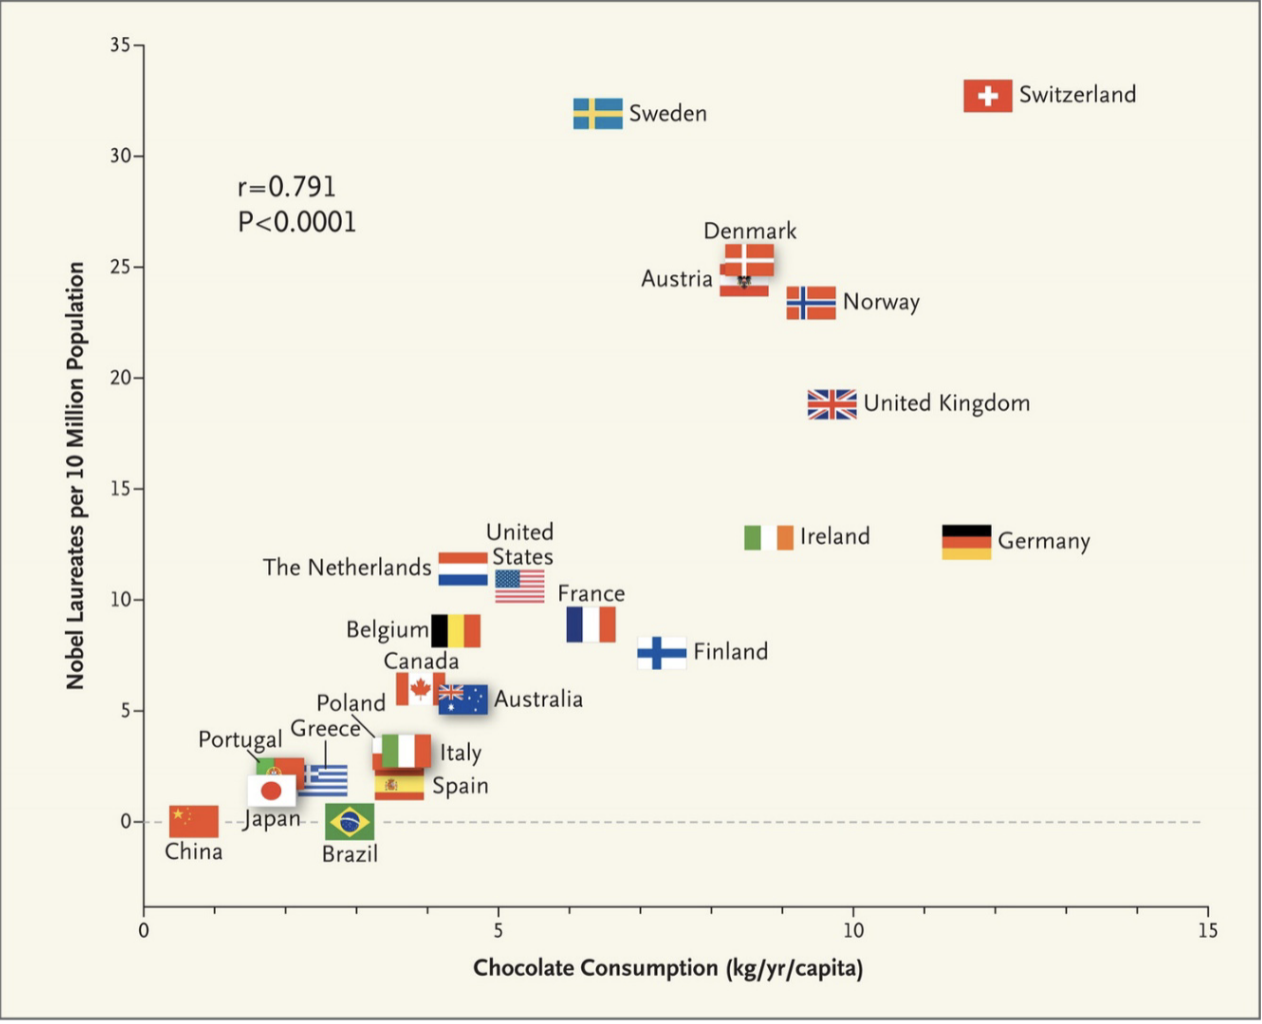
\includegraphics[width=0.65\linewidth]{images/01_chocolate} 

}

\caption{Chocolate Consumption and Nobel Prizes}\label{fig:chocolate}
\end{figure}

In Figure \ref{fig:chocolate}, the number of Nobel laureates per 10 million of the population (vertical axis) is plotted against the chocolate consumption in kilograms per capita in a given year (horizontal axis). As is clear in this graph, countries with higher rates of chocolate consumption also tend to have higher rates of Nobel laureates. This is an example of a \textbf{correlation}. A correlation is any statistical relationship between two variables.

Correlations can be very interesting. In many cases, they can lead to new research questions. But they don't often answer the questions social scientists are actually interested in. We are generally interested in understanding \textbf{causal relationships} between variables.

To understand causal relationships, let's again consider the relationship between chocolate consumption and Nobel prizes. Do you think that if the U.S. wanted to increase the number of Nobel laureates, they should invest in chocolate and include chocolate in lunch meals for students? Probably not! It's unlikely that increased chocolate consumption \textbf{causes} an individual to win a Nobel prize. In this case, it is more likely that this correlation in the data just arose due to chance. Therefore, we have uncovered a \textbf{spurious correlation}, which is defined as a correlation that arose due to chance. There are many interesting spurious correlations (See \href{https://www.tylervigen.com/spurious-correlations}{spurious-correlations}). For example, you probably would not guess that consumption of mozzarella cheese is correlated with civil engineering doctorates awarded, but see Figure \ref{fig:spurious} for this surprising correlation.

\begin{figure}

{\centering 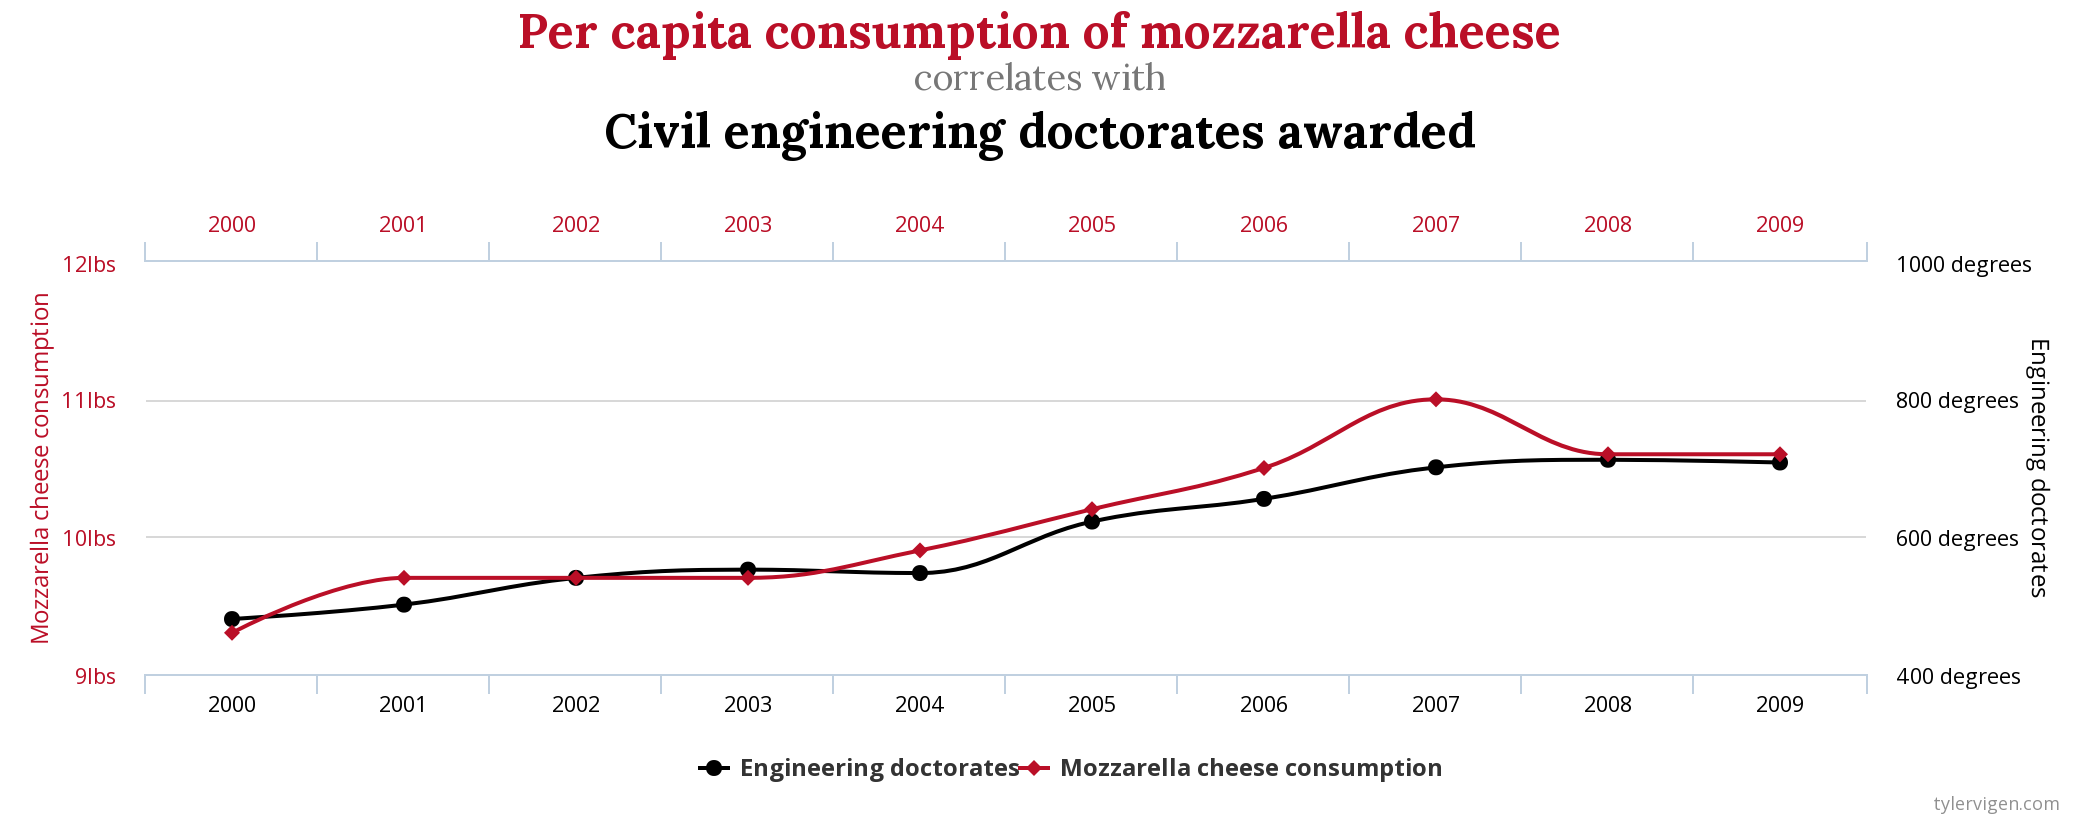
\includegraphics[width=1\linewidth]{images/01_spurious} 

}

\caption{Example of a Spurious Correlation from tylervigen.com}\label{fig:spurious}
\end{figure}

While spurious correlations can be interesting and fun, if we need to decide whether a given policy should be implemented, we need to understand how it causally impacts an individual's outcomes. To see why, let's imagine a high school is trying to decide whether to invest in a new after-school program designed to help students with standardized tests. Currently, they do not have such a program on campus, but they know some of their students attend programs offered outside the school. To try and understand the benefits of such a program, the school decides to use data to see if those who attended standardized test prep programs outperformed students who did not.

The school finds those who attended the test prep programs score much higher on standardized tests than those who didn't. Does this mean the test prep program works and the school should invest in one?

Maybe, maybe not. Two stories could potentially rationalize this finding. Story 1 is that the programs are effective ways for students to learn the material they need to perform well on standardized tests. That is, the program has a causal impact on SAT scores. Story 2 is that the programs are not actually effective. However, students who self-select into test prep programs also tend to be more motivated overall. They could, in theory, vary along many dimensions: academic ability, interest in college, parental background. It could be that any of these differences are actually driving the differences in standardized test scores.

With only \textbf{observational data} it is difficult to tell which story is true. However, there is a long-established way to identify causal relationships in medicine: the randomized control trial (RCT). To understand RCTs, imagine we are testing whether a given drug reduces blood pressure. To study the effectiveness we recruit a group of participants. Half of the participants are randomly placed into the \textbf{treatment} group and given the drug. The other half are placed into the \textbf{control} or \textbf{placebo} group and given a placebo drug. Now we can just compare outcomes for the two groups over time to understand the impact of the drug.

The key to a well-done experiment is \textbf{randomization}. If who receives the treatment is completely random, then on average, the two groups will be very similar. For example, in our test prep example, if we could randomly split students into two groups: test prep vs.~no test prep, then we could evaluate the impacts of the program. Since students are no longer self-selecting into the program, there should be little difference between the two groups in terms of academic ability, college interest, parental background. Why would there be? We randomized the students into the program.

Not all questions in social science can be answered with an experiment. In certain cases, it may be prohibitively expensive or unethical to run an experiment. However, if an experiment can be done, it is hard to find more convincing evidence. Experiments have been widely influential in many social sciences. For example, in the field of development economics, a large number of experiments have been undertaken to develop policies aimed at alleviating global poverty. In 2019, Abhijit Banerjee, Esther Duflo, and Michael Kremer won the Nobel Prize in Economics ``for their experimental approach to alleviating global poverty.''

In this course, we will be studying a number of social science experiments. Our first experiment comes from Brownback and Sadoff (2020). The motivation for this experiment is a startling statistic. Only 40 percent of community college students earn a college degree within 6 years (Shapiro et al.~2017). Given these poor outcomes, it is important to consider tools to improve performance. In Brownback and Sadoff (2020) the researchers explore one potential tool that has been previously unexplored: financial incentives to instructors. This is often referred to as a pay-for-performance model. Instructors are paid for how well their students perform.

To get specific, Brownback and Sadoff (2020) ran the following experiment at a community college in Indiana (Ivy Tech):

\begin{itemize}
\tightlist
\item
  Some instructors (the treatment group) received \$50 for each student that passed an externally-administered test
\item
  Other instructors (the control group) did not receive such an incentive.
\end{itemize}

The key in their design is that the instructors that are chosen to receive the incentives are randomly selected. Therefore, they are not, on average, better teachers than instructors in the control group. Therefore, if we observe any difference in student performance between the treatment and control, then it must be due to the financial incentives for instructors!

\textbf{Question: The key aspect of an experiment that allows us to infer causation is\ldots{}}

\begin{itemize}
\tightlist
\item
  \begin{enumerate}
  \def\labelenumi{(\Alph{enumi})}
  \tightlist
  \item
    Ability to randomize individuals across treatment and control\\
  \end{enumerate}
\item
  \begin{enumerate}
  \def\labelenumi{(\Alph{enumi})}
  \setcounter{enumi}{1}
  \tightlist
  \item
    Ability to collect large amounts of data\\
  \end{enumerate}
\item
  \begin{enumerate}
  \def\labelenumi{(\Alph{enumi})}
  \setcounter{enumi}{2}
  \tightlist
  \item
    Ability to follow individuals over time\\
  \end{enumerate}
\item
  \begin{enumerate}
  \def\labelenumi{(\Alph{enumi})}
  \setcounter{enumi}{3}
  \tightlist
  \item
    Ability to collect information about confounding variables
  \end{enumerate}
\end{itemize}

\section{Community College Data}\label{community-college-data}

In many disciplines, there has been a push toward transparency and replication. Past work has shown that some very influential studies have failed to replicate (see \href{https://en.wikipedia.org/wiki/Replication_crisis\#In_economics}{here}). A common way to provide transparency is to have authors make the data from their research publicly available. That means we will get to use the actual data from the experiments we are studying in this class.

Table \ref{fig:bsdata} shows a selection of the data from Brownback and Sadoff (2020). The actual data is much larger, but only a subset of the variables will be relevant for our analysis. This is referred to as a \textbf{data table}. Each \textbf{row} in a data table is an \textbf{observation}, while each \textbf{column} is a \textbf{variable}.

\begin{figure}

{\centering 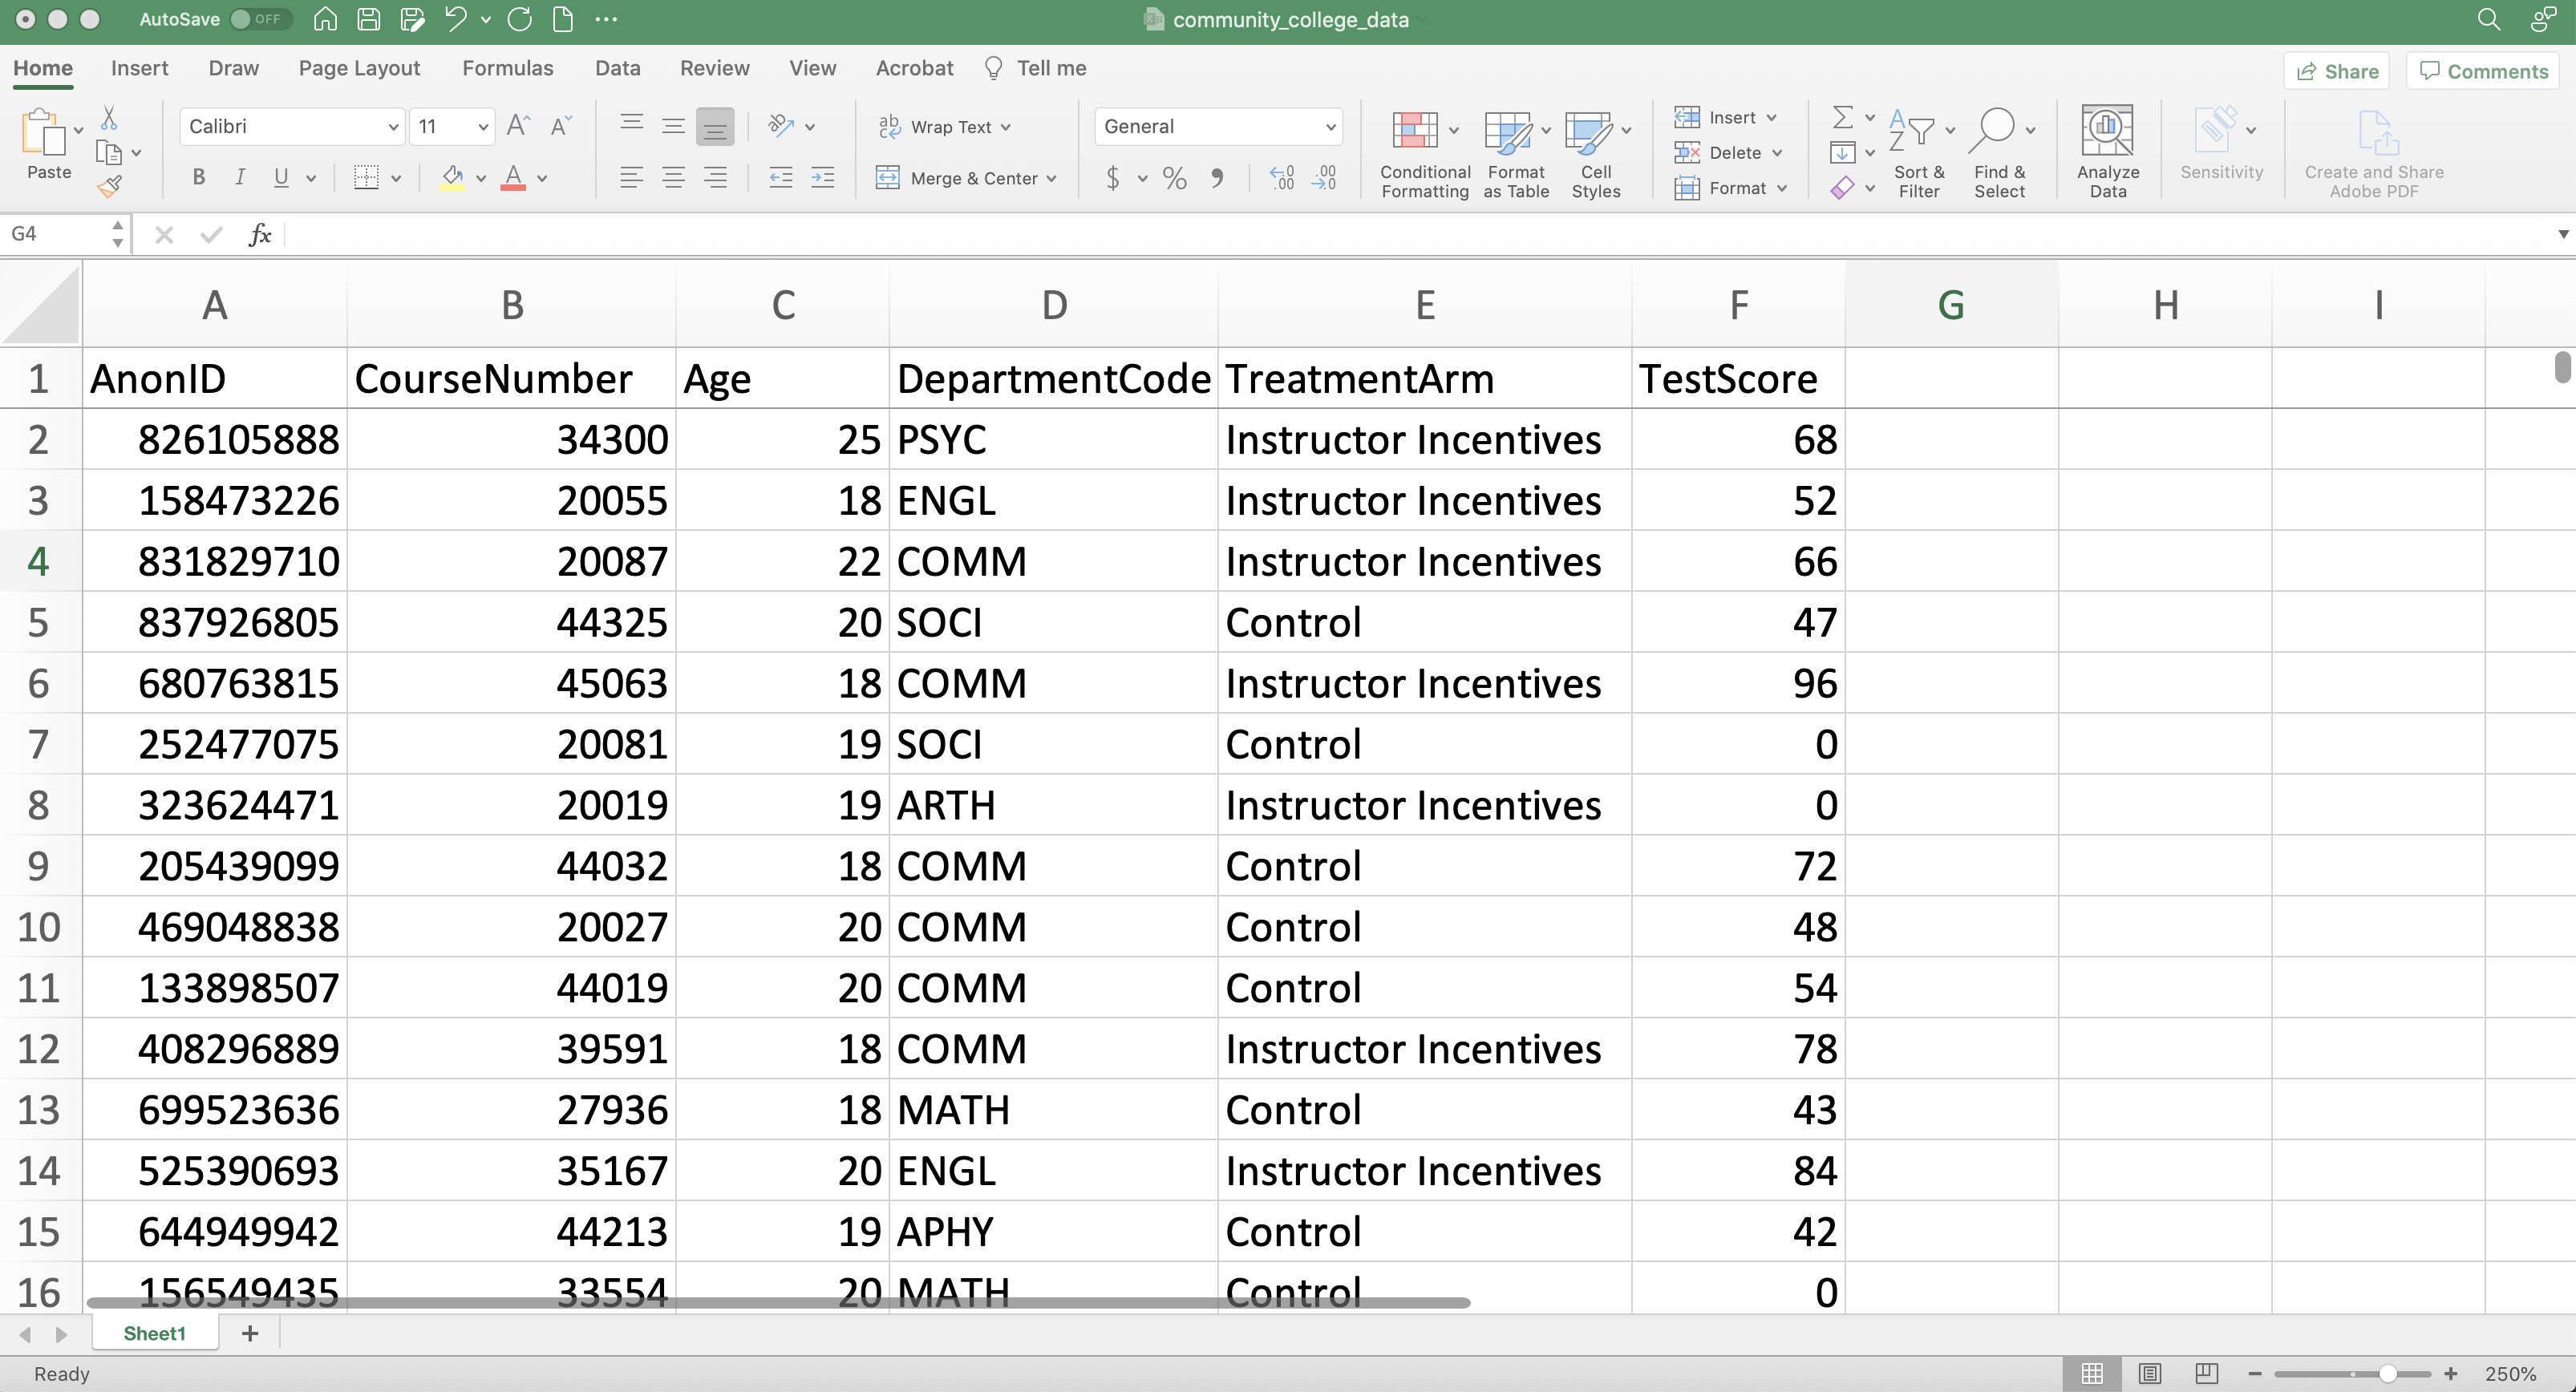
\includegraphics[width=0.75\linewidth]{images/01_data} 

}

\caption{Data From Brownback and Sadoff (2020)}\label{fig:bsdata}
\end{figure}

It is always important to understand the structure of your data before proceeding with any data analysis. One of the most important components of understanding the structure is to discern the \textbf{unit of observation}. The unit of observation is the level at which the data is reported. To discern it for yourself, just think about what each row of the dataset represents. Is each row an individual, a neighborhood, a state, or a country? To practice, let's go through a few examples.

What is the unit of observation in Figure \ref{fig:student}, which displays a data table for just two observations?

\begin{figure}

{\centering 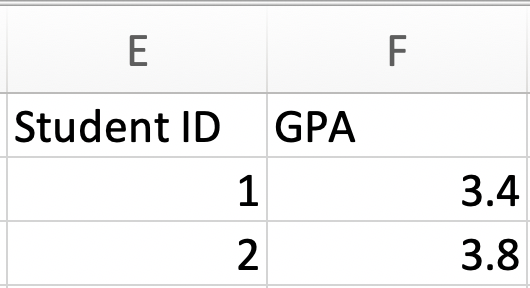
\includegraphics[width=0.5\linewidth]{images/01_student} 

}

\caption{Unit of Observation Example 1}\label{fig:student}
\end{figure}

To answer this question, we need to decide what a row represents. In this case, each row corresponds to a different student. Therefore the observation level is a student.

What is the unit of observation in Figure \ref{fig:studentterm}?

\begin{figure}

{\centering 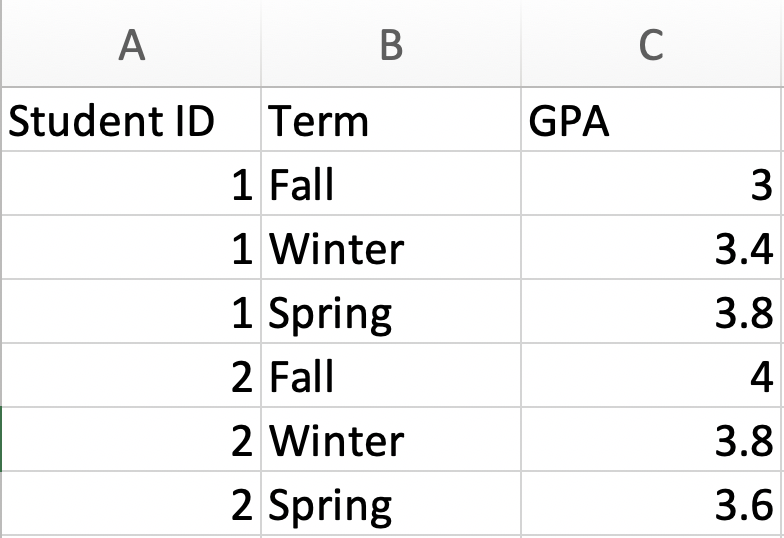
\includegraphics[width=0.55\linewidth]{images/01_student_term} 

}

\caption{Unit of Observation Example 2}\label{fig:studentterm}
\end{figure}

Again, we need to decide what a row represents. In this case, each row corresponds to a particular student in a particular term. Therefore the observation level is a student-term.

Now let's think about what the unit of observation is in the Brownback and Sadoff (2020) data. The variable \textbf{AnonID} is the identifier for a student. The variable \textbf{CourseNumber} is the identifier for a course. This dataset seems to be giving us the information for a student in a given course. Therefore the observation level is a student-course.

Before we get to analyzing the data, let's actually learn about our first feature in Excel. When browsing an excel file, it is often convenient to \textbf{freeze} the first row so that it is always visible. In our case, the first row holds variable names. Therefore, if we freeze the first row we can scroll through the data without having to remember what each column corresponds to.

To freeze the first row go to the \textbf{View} and then click \textbf{Freeze Top Row}.

\begin{figure}

{\centering 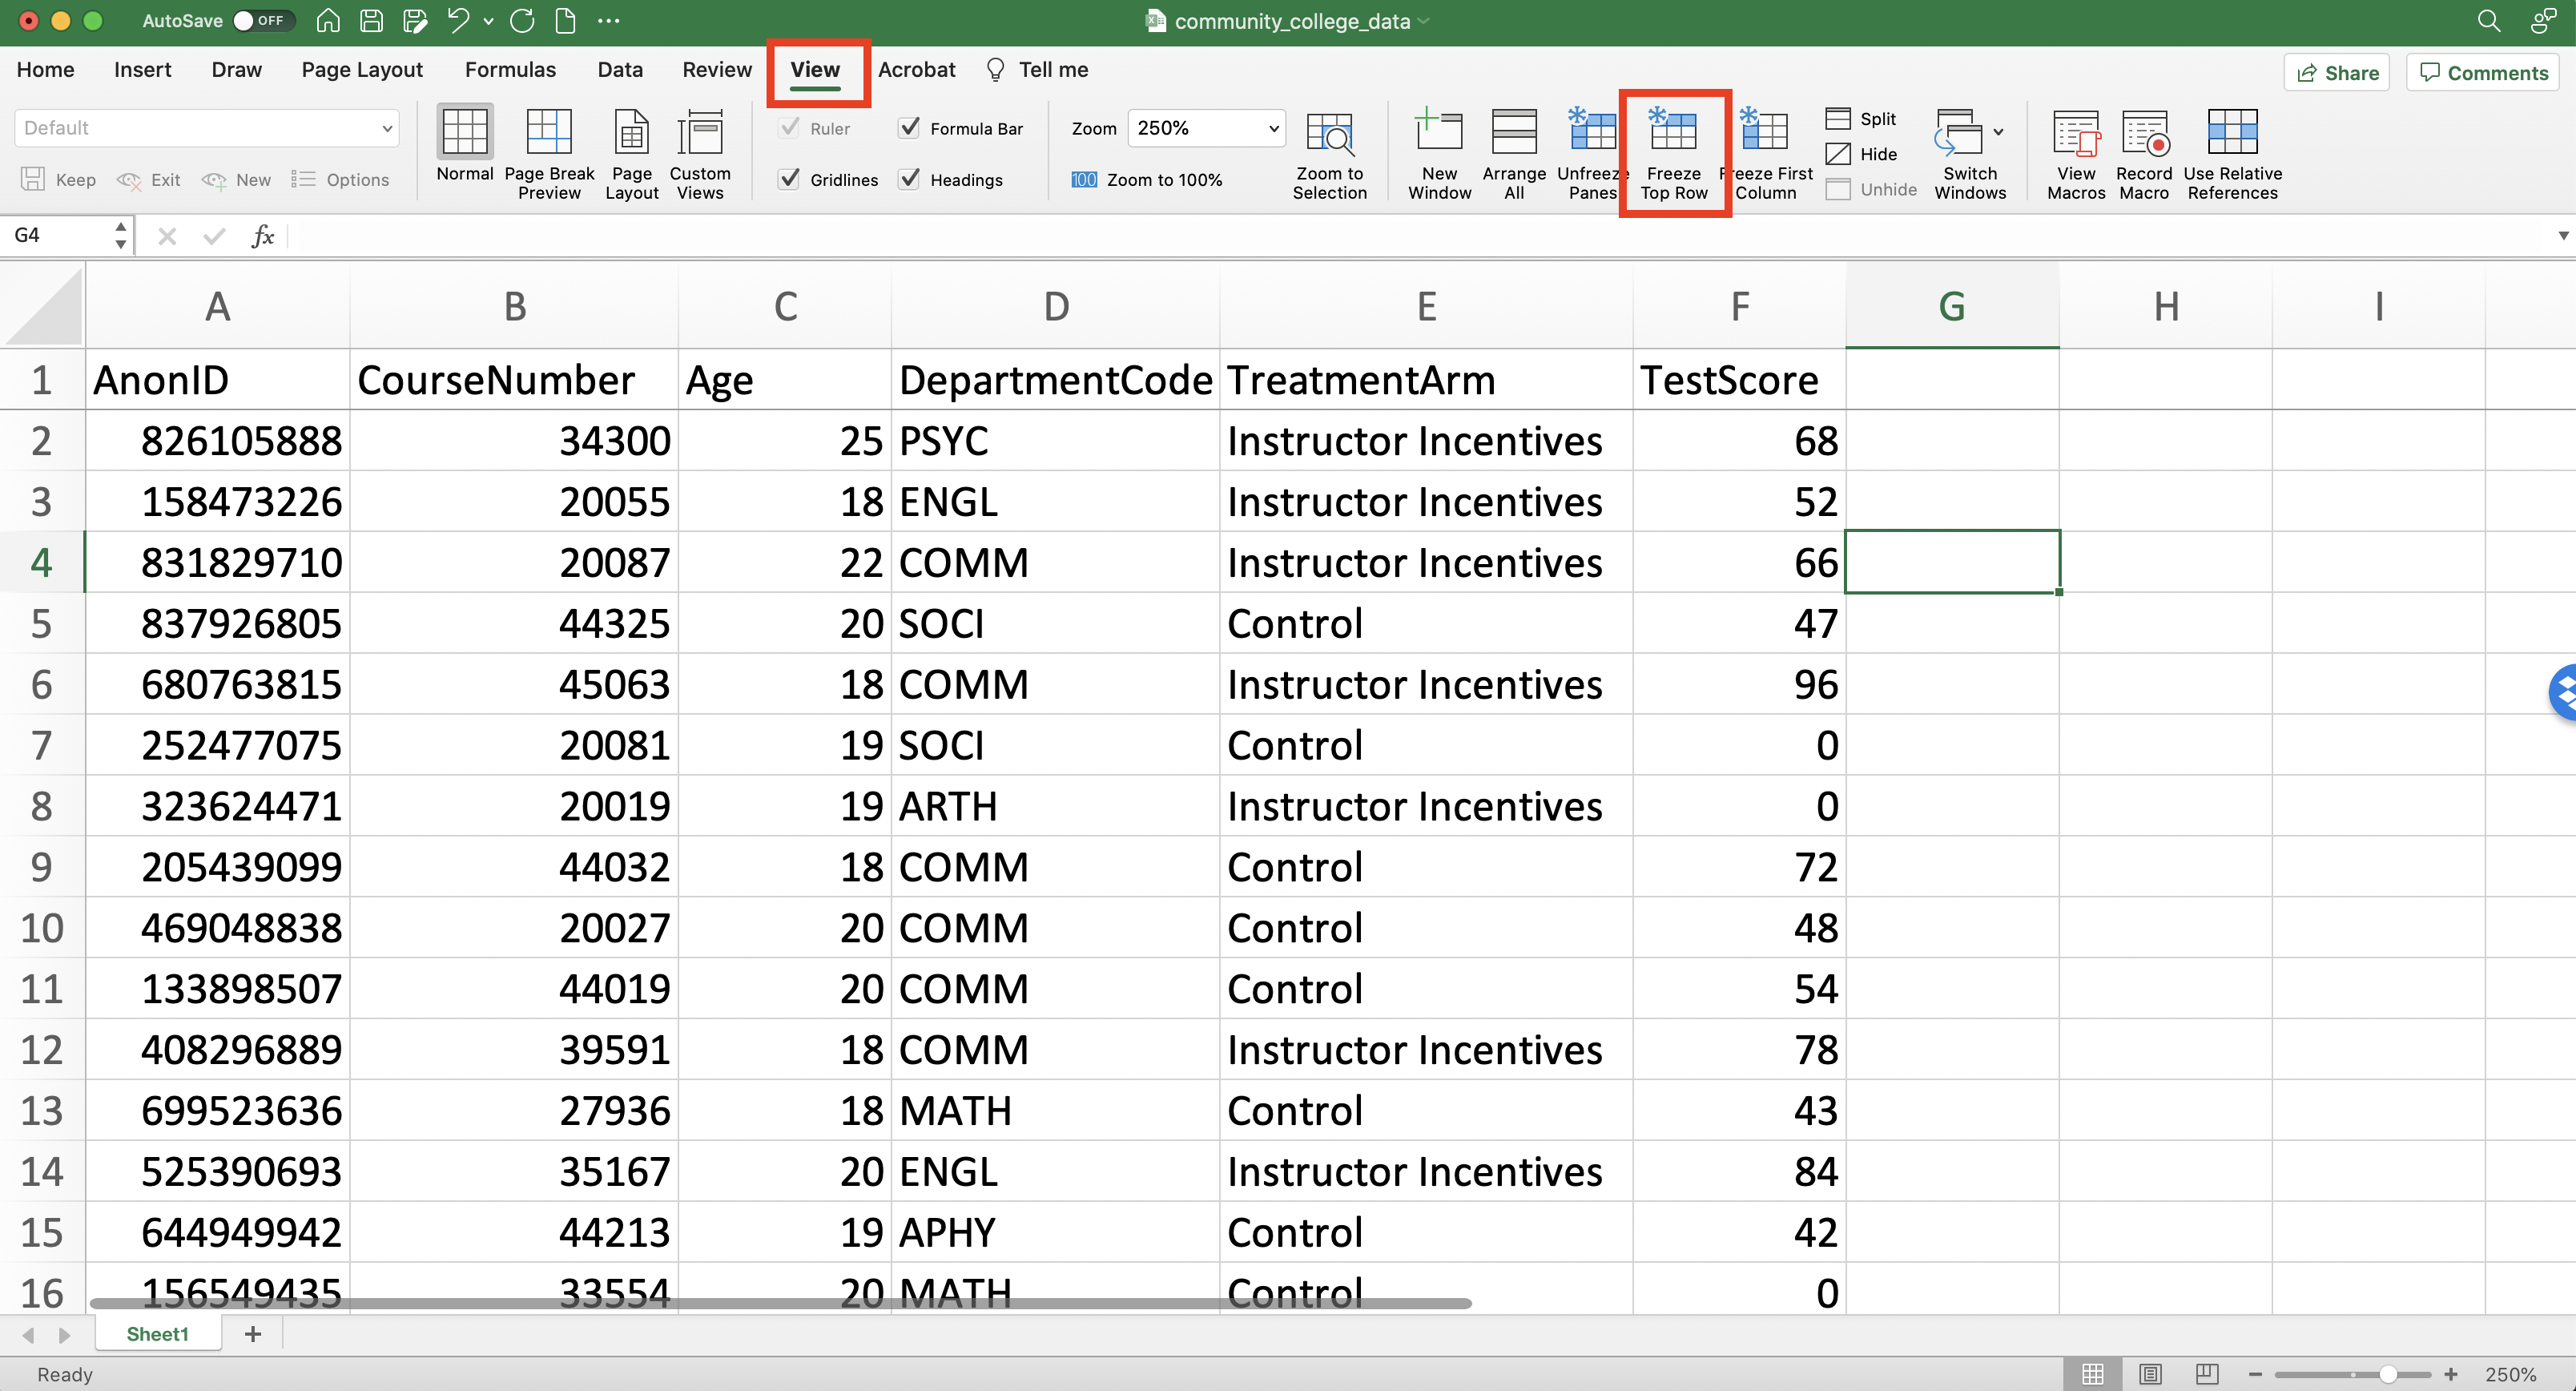
\includegraphics[width=1\linewidth]{images/01_freeze} 

}

\caption{Freezing the First Row}\label{fig:freeze}
\end{figure}

Let's talk a little bit about our goal with this dataset. Our goal is to determine if providing financial incentives to teachers impacts student performance. The variable \textbf{Treatment Arm} details whether a student has an instructor who received incentives or is in the control group. Therefore, we can see if test scores improve based on the Treatment Arm of the student. To perform this analysis, we need to learn how to use \textbf{functions} in Excel.

\textbf{Question: Imagine we have a dataset where each row contains the average unemployment rate for a given state in a given year. The unit of observation in this dataset is}

\begin{itemize}
\tightlist
\item
  \begin{enumerate}
  \def\labelenumi{(\Alph{enumi})}
  \tightlist
  \item
    State\\
  \end{enumerate}
\item
  \begin{enumerate}
  \def\labelenumi{(\Alph{enumi})}
  \setcounter{enumi}{1}
  \tightlist
  \item
    Year\\
  \end{enumerate}
\item
  \begin{enumerate}
  \def\labelenumi{(\Alph{enumi})}
  \setcounter{enumi}{2}
  \tightlist
  \item
    Individual-year\\
  \end{enumerate}
\item
  \begin{enumerate}
  \def\labelenumi{(\Alph{enumi})}
  \setcounter{enumi}{3}
  \tightlist
  \item
    State-year
  \end{enumerate}
\end{itemize}

\section{Statistical Functions}\label{statistical-functions}

A function is something that takes in an input and produces an output. For example, you can think of taking the average as a function. The input is a list of numbers, and the output is the average of that list of numbers. When the inputs and outputs of a function are numbers, then it is a \textbf{statistical function}.

In Excel, statistical functions are extremely important to understand. If you are doing research, it is common to start with a list of summary statistics. If you are in a business, it might be important to know some summary statistics about your products. To create these summary statistics we use statistical functions.

In order to illustrate the use of statistical functions, let's consider the following dataset that has information on Gross Domestic Product (GDP) for ten countries

\begin{figure}

{\centering 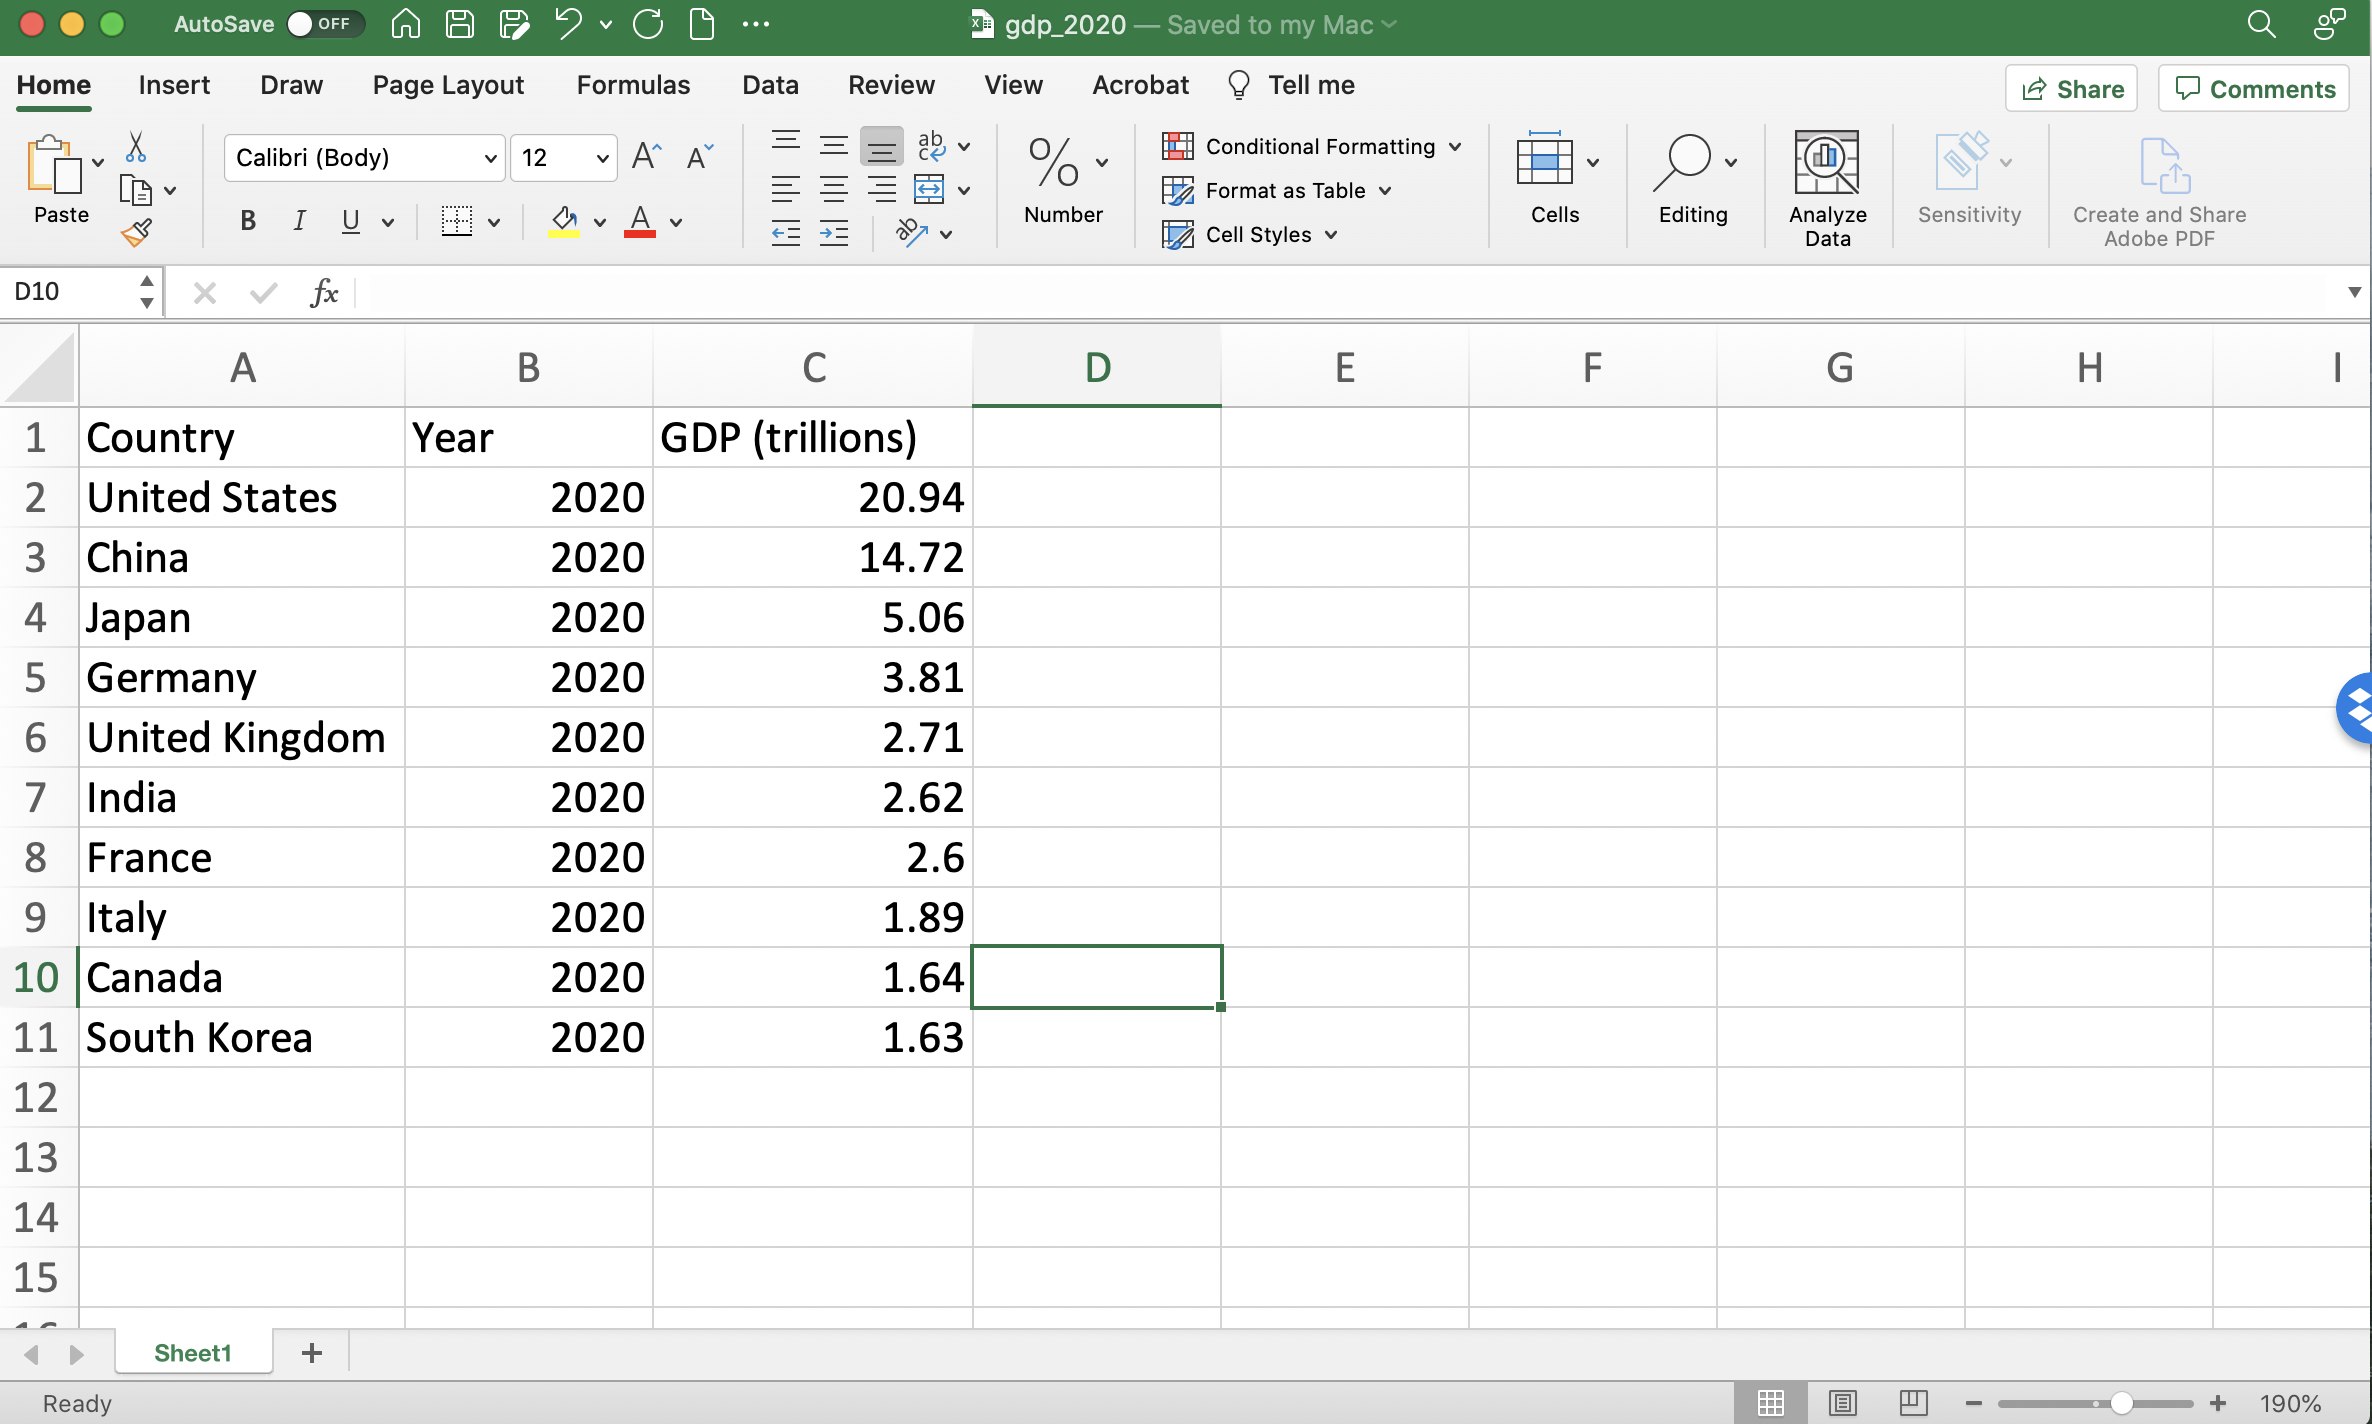
\includegraphics[width=1\linewidth]{images/01_gdp2020} 

}

\caption{GDP in 2020}\label{fig:gdp2020}
\end{figure}

Let's introduce our first statistical function: the \texttt{AVERAGE} function. This function will take in a list of numbers and output the average of all those numbers. There are many statistical functions in Excel, including:

\begin{itemize}
\item
  \texttt{COUNT} -- counts the number of numbers
\item
  \texttt{SUM} -- adds up the numbers
\item
  \texttt{MEDIAN} -- retrieves the median of all numbers
\item
  \texttt{MAX}, \texttt{MIN} -- retrieves the maximum and minimum of all numbers
  respectively
\item
  \texttt{MODE} -- retrieves the mode of all numbers
\end{itemize}

To make use of statistical functions, we first need to learn how to reference cells. In Excel, every cell is identified by a column letter and a row number. For example, in Figure \ref{fig:japan}, I have clicked on the cell that holds the word ``Japan''. This entry is in column A of row 4. Therefore, this is cell A4.

\begin{figure}

{\centering 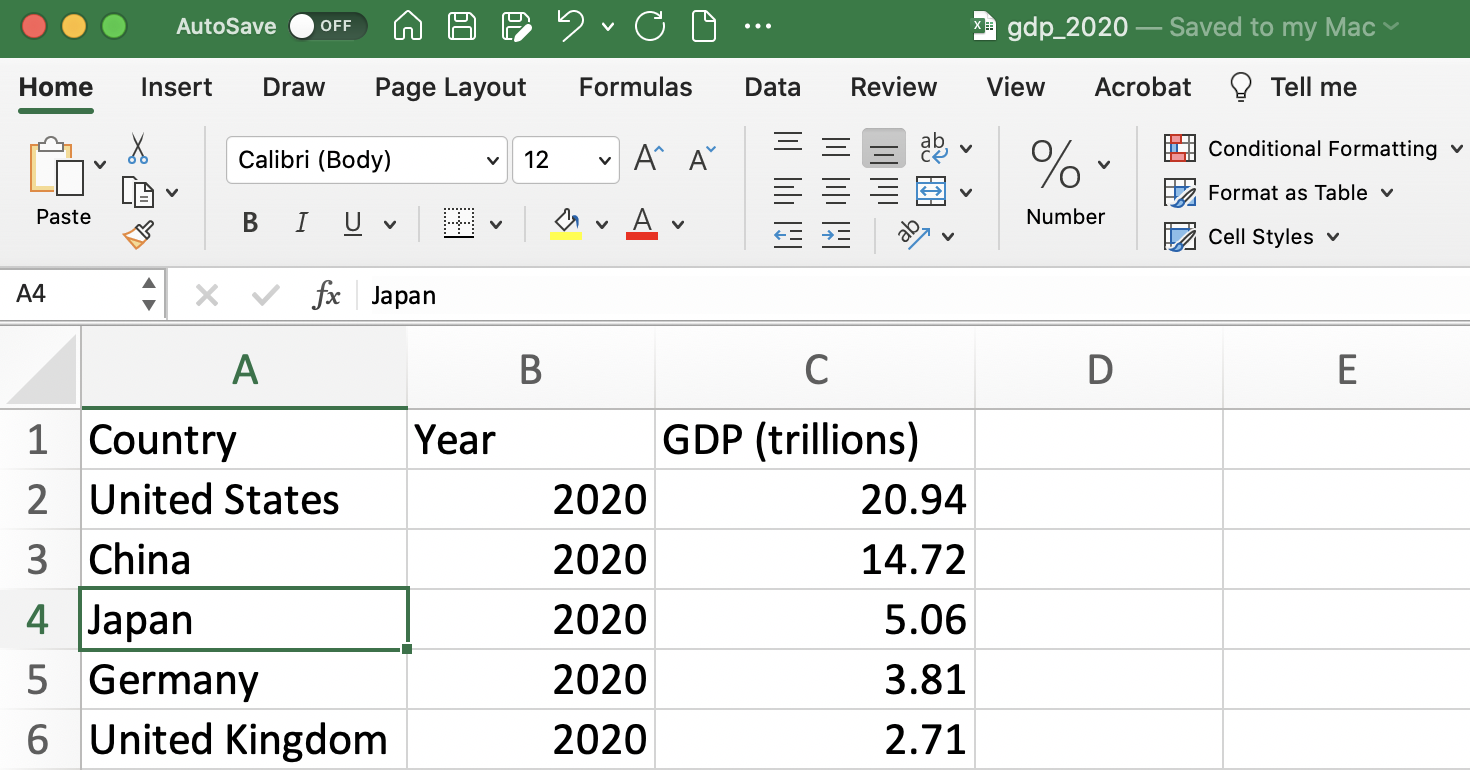
\includegraphics[width=1\linewidth]{images/01_japan} 

}

\caption{How to Reference a Cell}\label{fig:japan}
\end{figure}

You can also reference a range of cells (this will be useful when taking averages). For example, to reference rows 2-6 of column C we could type \texttt{C2:C6} (See Figure \ref{fig:cells}). Whenever you read a colon in Excel, you should read it as ``through''. Therefore, the text \texttt{C2:C6} can be read as ``cells C2 through C6''.

\begin{figure}

{\centering 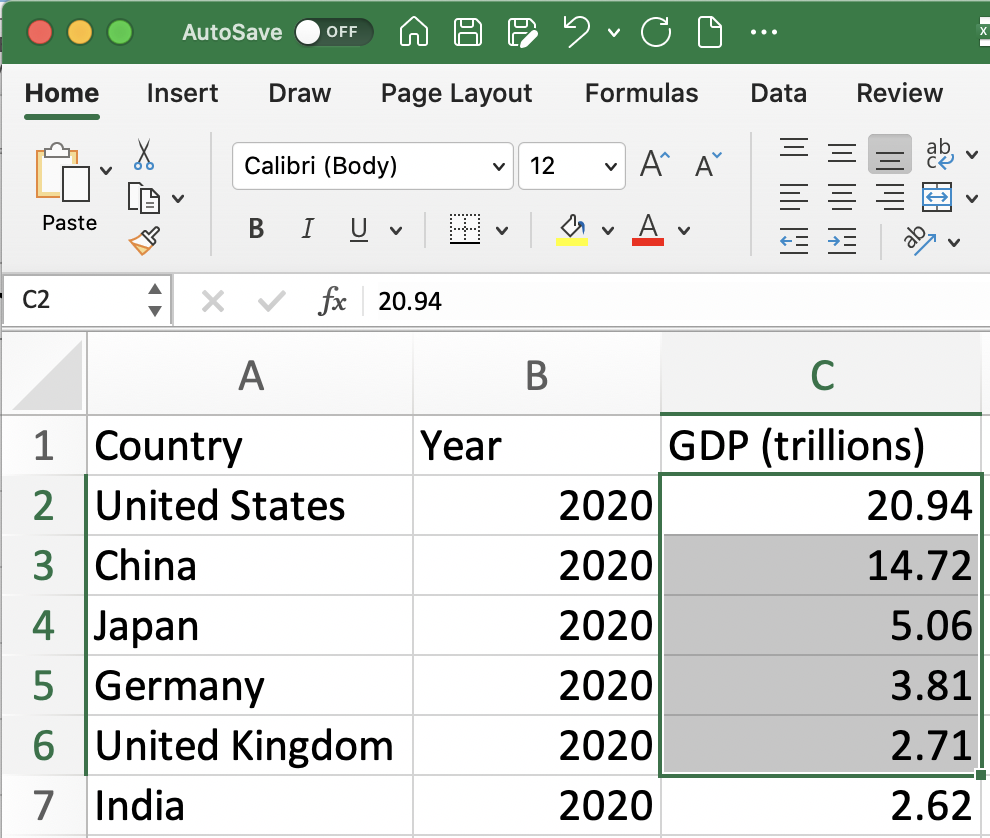
\includegraphics[width=0.7\linewidth]{images/01_cells} 

}

\caption{Referencing a Range of Cells}\label{fig:cells}
\end{figure}

Sometimes, it is helpful to reference an entire column. For example, later we will open an Excel spreadsheet that has thousands of students, which might make it difficult to reference the exact row at which the data ends. We can still very compactly take the average of this variable without referencing all the observations. For example, if the variable is in column C, we can type \texttt{C:C} to reference the entire column.

Now that we understand how to reference cells, we can begin to apply functions. We will begin with the \texttt{AVERAGE} functions which can compute an average of a list of numbers. In our spreadsheet, we are interested in computing the average GDP across these ten countries. To do so, we can first click in an unpopulated cell (i.e.~a cell without any values in it yet) and type:

\begin{center}
\colorbox{gray!20}{\texttt{=AVERAGE(C:C)}}
\end{center}

Note the \texttt{=} sign in the text above. This tells Excel to evaluate the function. If you omit the \texttt{=} you will find that the cell is just populated with the text \texttt{AVERAGE(C:C)} and not the average value of column C.

Figure \ref{fig:average1} depicts an example where we have set up a Summary Statistics table for this dataset. In cell F3, we have written the function that calculates the average GDP across these ten countries.

\begin{figure}

{\centering 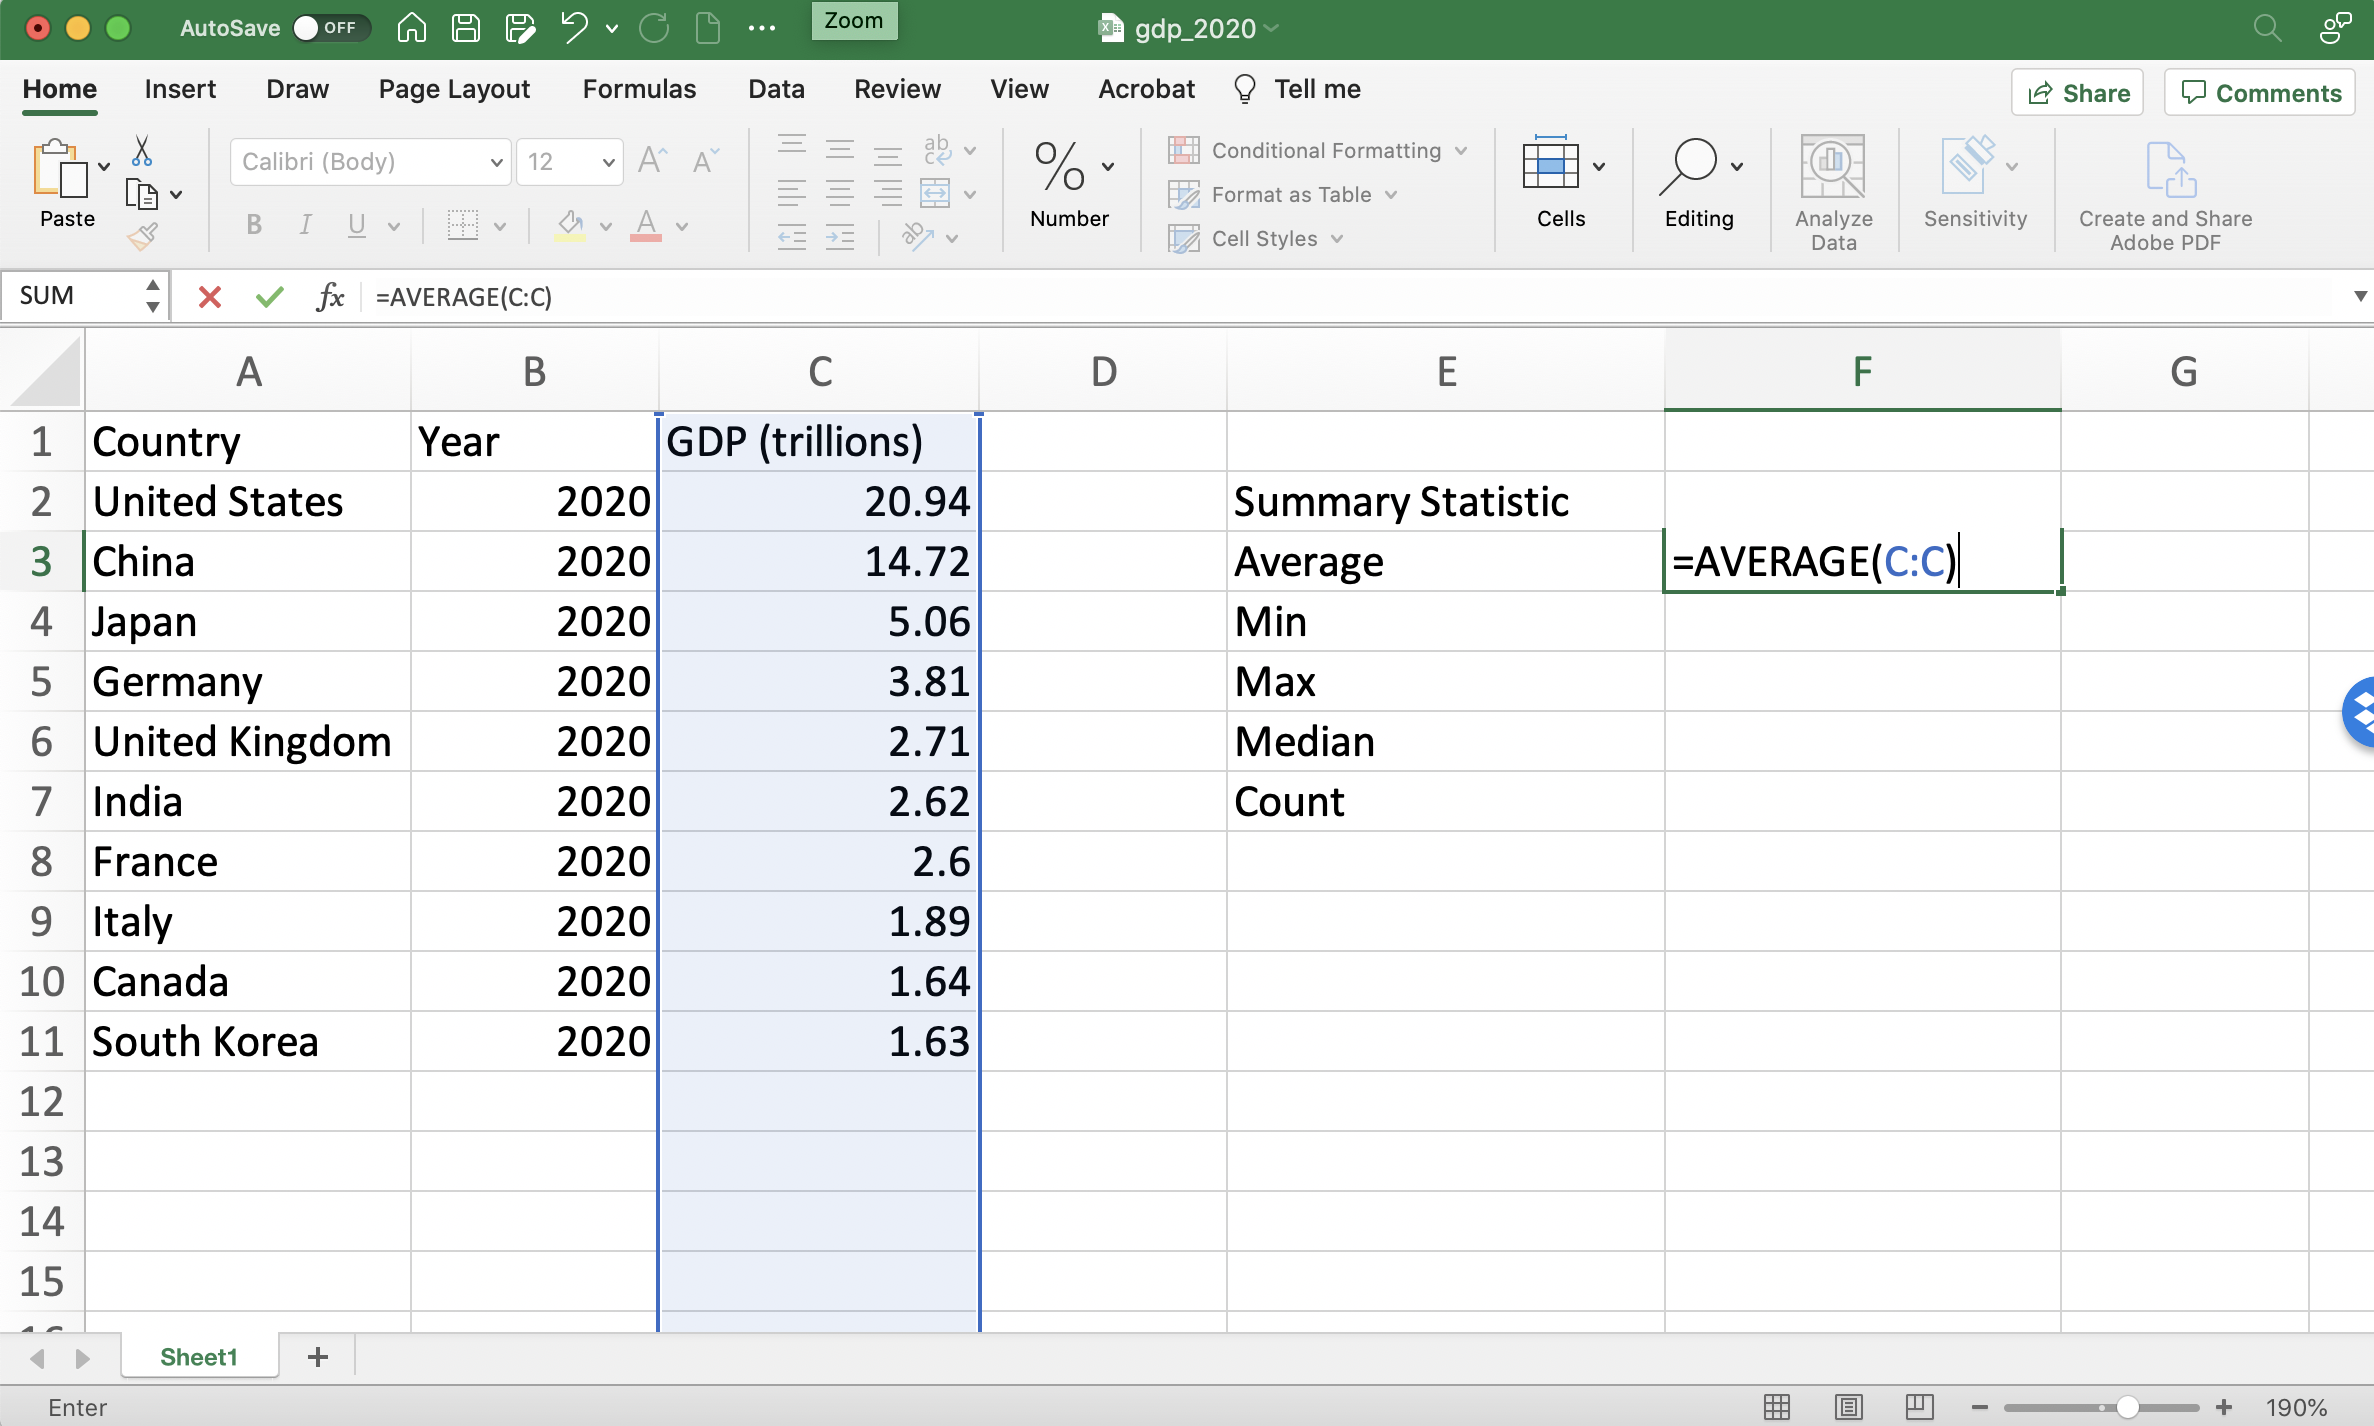
\includegraphics[width=0.8\linewidth]{images/01_average1} 

}

\caption{Computing Average GDP in 2020 (Before Pressing Enter)}\label{fig:average1}
\end{figure}

As soon as we press enter, the function will be evaluated and the average will appear in cell F3 (see Figure \ref{fig:average2}).

\begin{figure}

{\centering 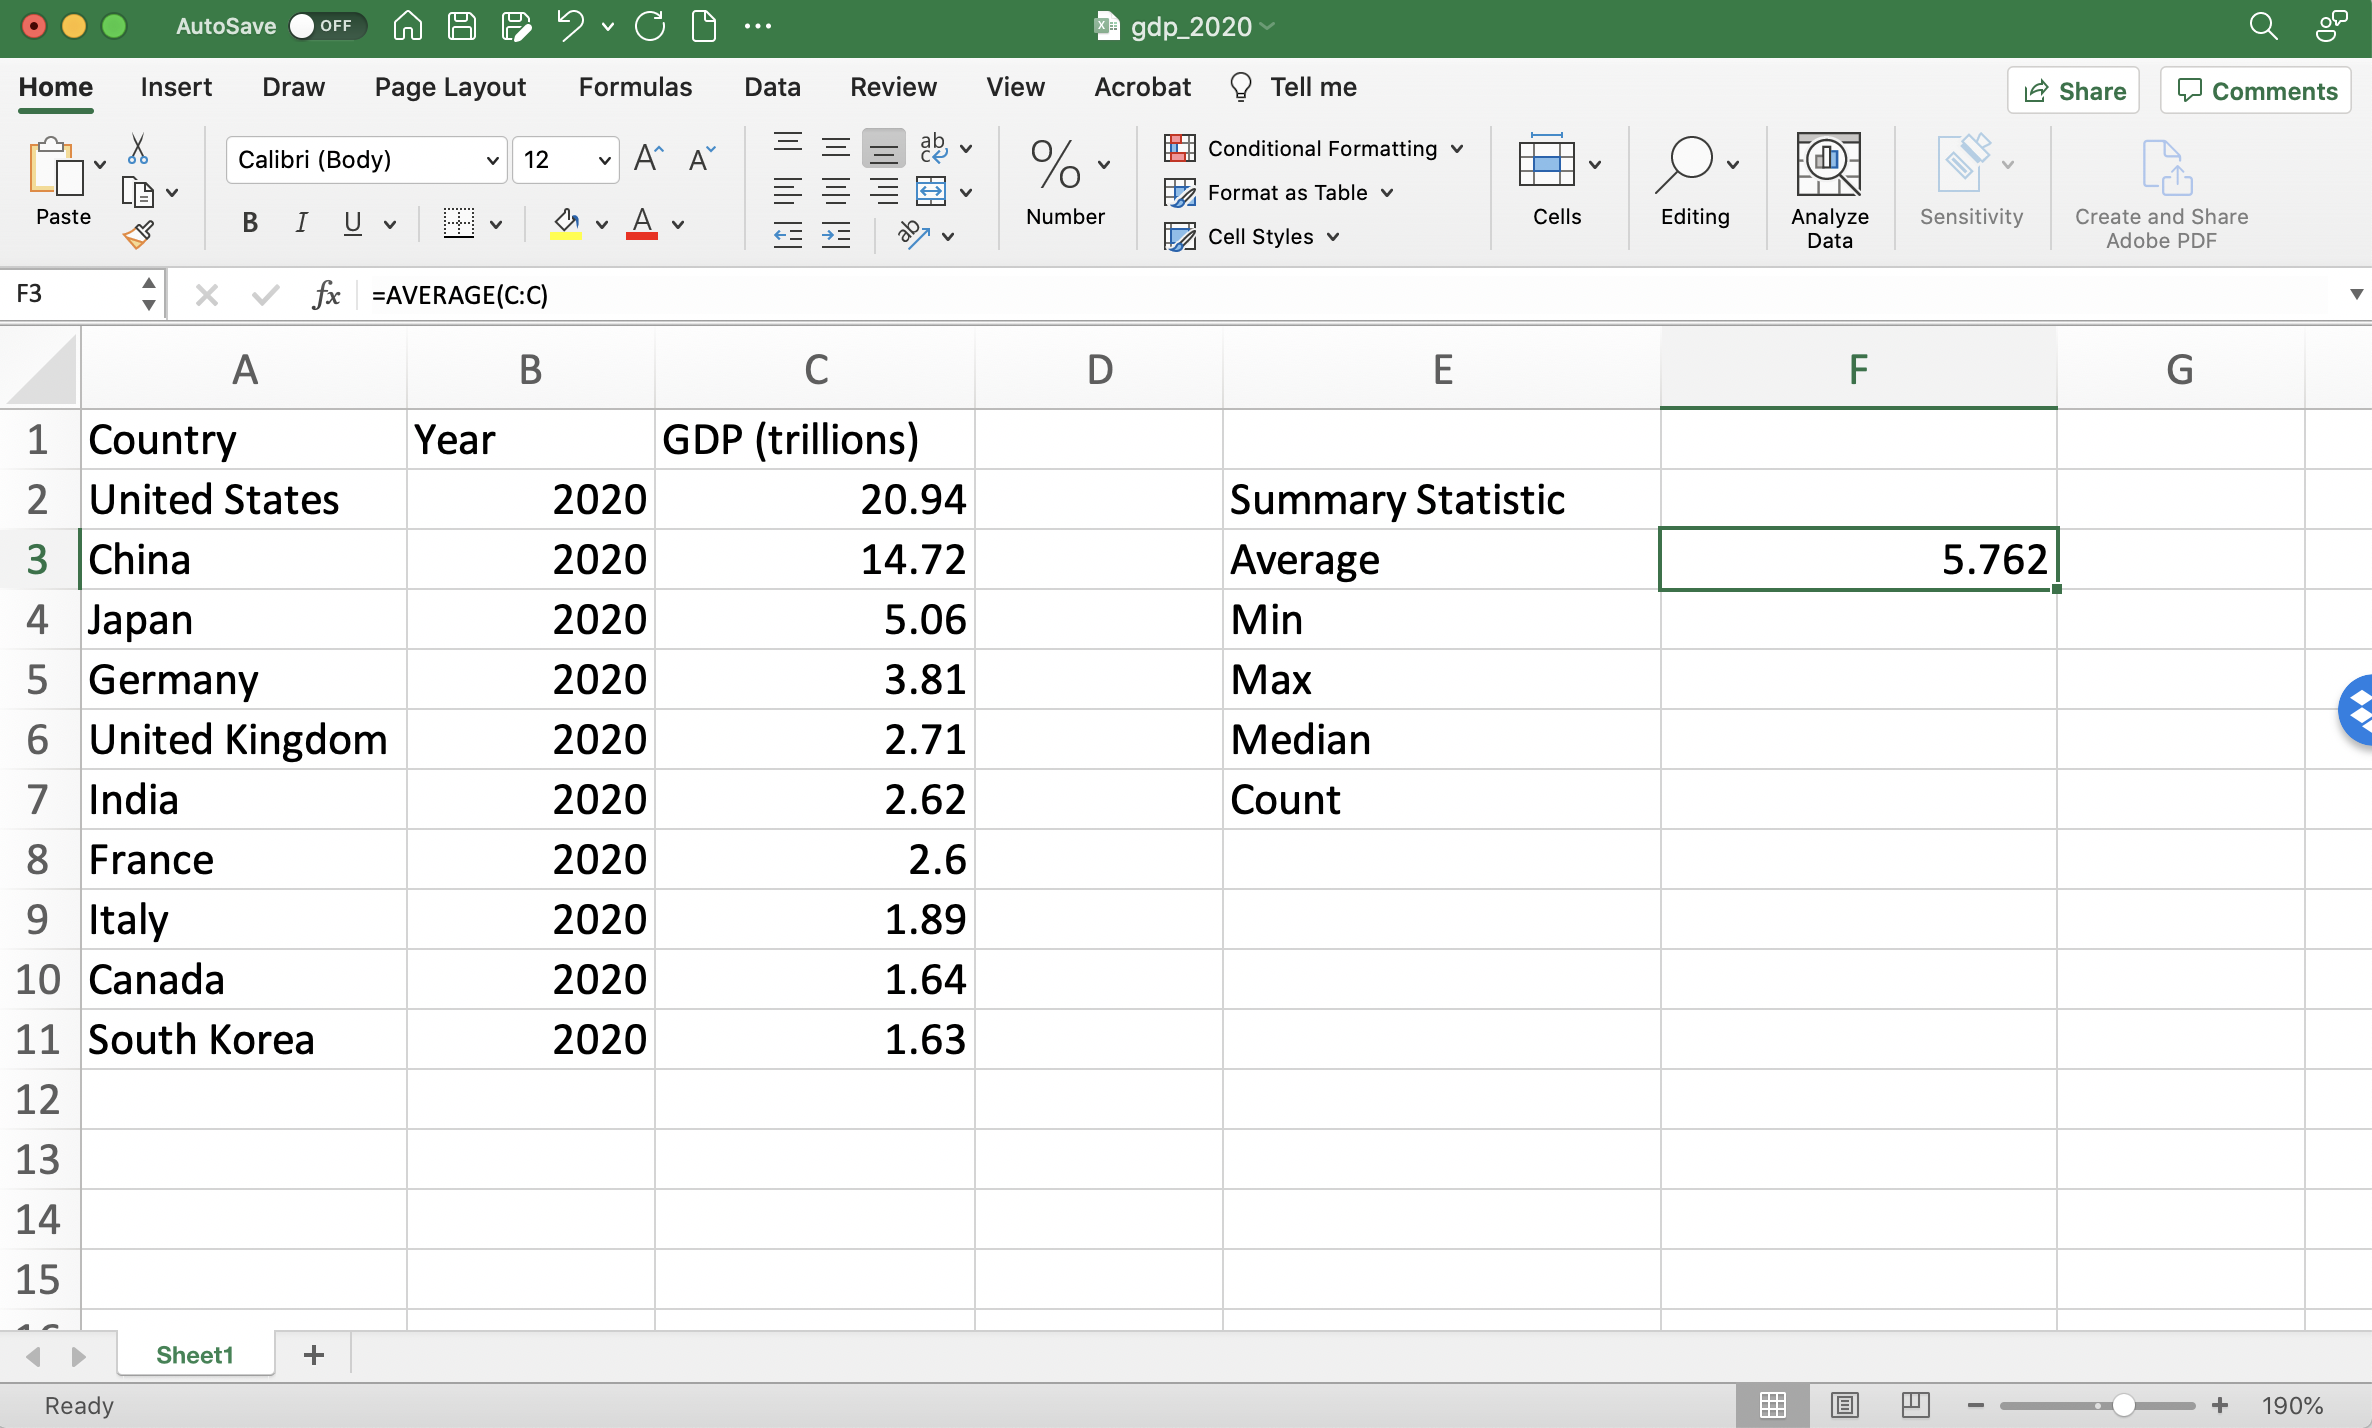
\includegraphics[width=0.8\linewidth]{images/01_average2} 

}

\caption{Computing Average GDP in 2020 (After Pressing Enter)}\label{fig:average2}
\end{figure}

The rest of the summary statistics are completely analogous, replacing \texttt{AVERAGE} with the relevant function. See Figure \ref{fig:gdpsumstats} for the output of the rest of the Summary Statistics table.

\begin{figure}

{\centering 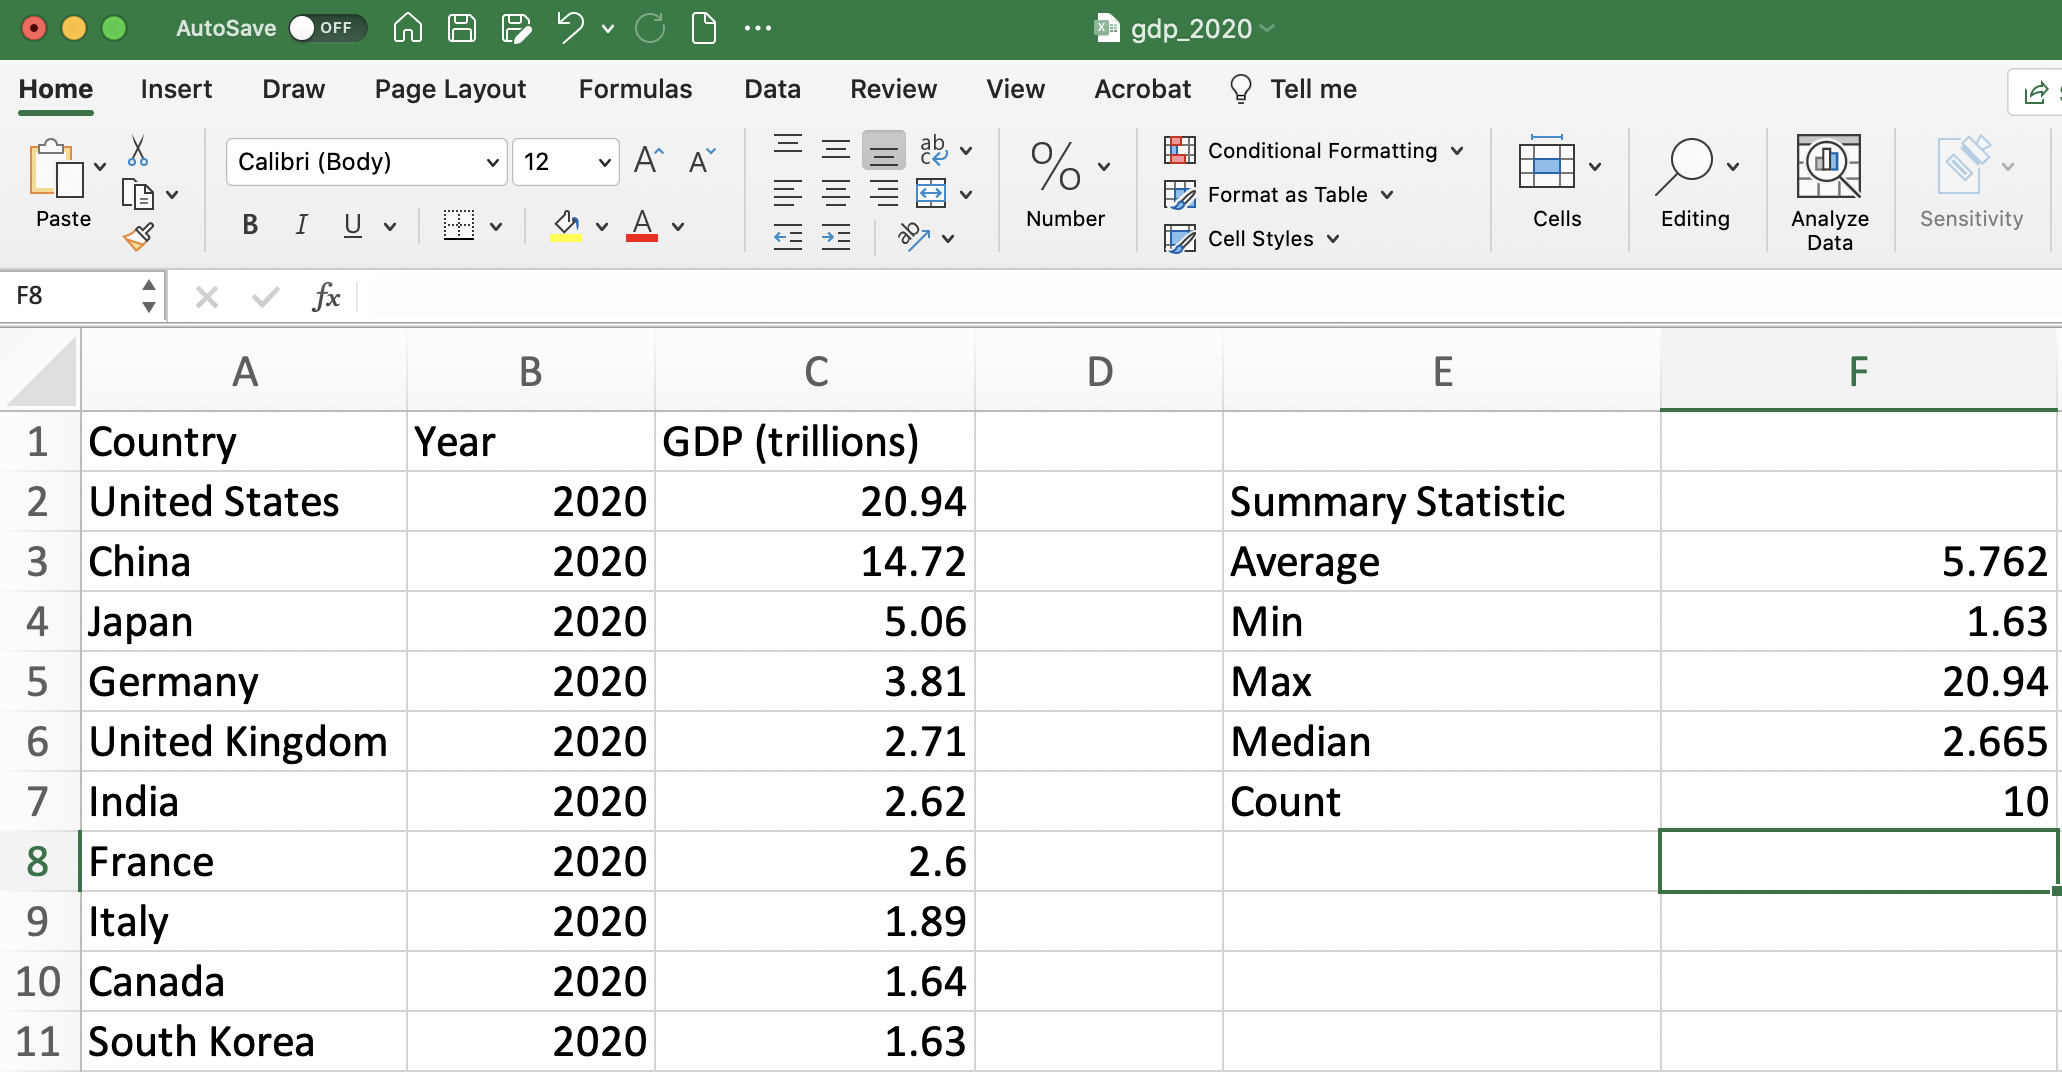
\includegraphics[width=0.8\linewidth]{images/01_gdp_sum_stats} 

}

\caption{Summary Statistics Table}\label{fig:gdpsumstats}
\end{figure}

\textbf{Question: I try to take the AVERAGE of a column by specifying \texttt{AVERAGE(C:C)}. Yet, when I press enter, Excel does not compute the average. What has gone wrong}

\begin{itemize}
\tightlist
\item
  \begin{enumerate}
  \def\labelenumi{(\Alph{enumi})}
  \tightlist
  \item
    AVERAGE is the wrong function to use\\
  \end{enumerate}
\item
  \begin{enumerate}
  \def\labelenumi{(\Alph{enumi})}
  \setcounter{enumi}{1}
  \tightlist
  \item
    Column C must not be numeric\\
  \end{enumerate}
\item
  \begin{enumerate}
  \def\labelenumi{(\Alph{enumi})}
  \setcounter{enumi}{2}
  \tightlist
  \item
    Need to specify equals sign \texttt{=} before the function
  \end{enumerate}
\end{itemize}

\section{Logical Functions}\label{logical-functions}

Another type of function in Excel is called a \textbf{logical function}. Before learning about \textbf{logical functions} we need to learn more about logical statements in general. A logical statement is a statement that is either true or false. For example, all of the following statements are either true or false.

\begin{itemize}
\item
  ``The student passed the class''
\item
  ``The participant is in the treatment group''
\item
  ``The temperature is below freezing''
\end{itemize}

These statements are all either true or false. This type of binary logic is incredibly important in certain areas of mathematics as well as the development of computers. An entire branch of mathematics, termed \textbf{Boolean algebra}, deals with variables that take on binary values.

In Excel, we can type logical statements and Excel will evaluate whether the statement is True or False. The key is you need to type the statement in the correct format so that Excel understands what you are trying to ask.

For example, in our dataset on GDP in 2020, a logical statement is: ``GDP is greater than 10 trillion dollars.'' This is True for some countries and False for others. But how do we type the statement ``GDP is greater than 10 trillion dollars'' in Excel?

Figure \ref{fig:tf1} depicts how we would type this statement for the first observation in the dataset (the U.S.). To evaluate whether GDP is greater than 10 trillion for the U.S. we type \texttt{=(C2\textgreater{}10)}. The equals sign tells Excel to evaluate the logical statement that follows. The logical statement that follows \texttt{C2\textgreater{}10} is simply asking whether the value in cell C2 (i.e.~U.S.'s GDP) is greater than 10.

\begin{figure}

{\centering 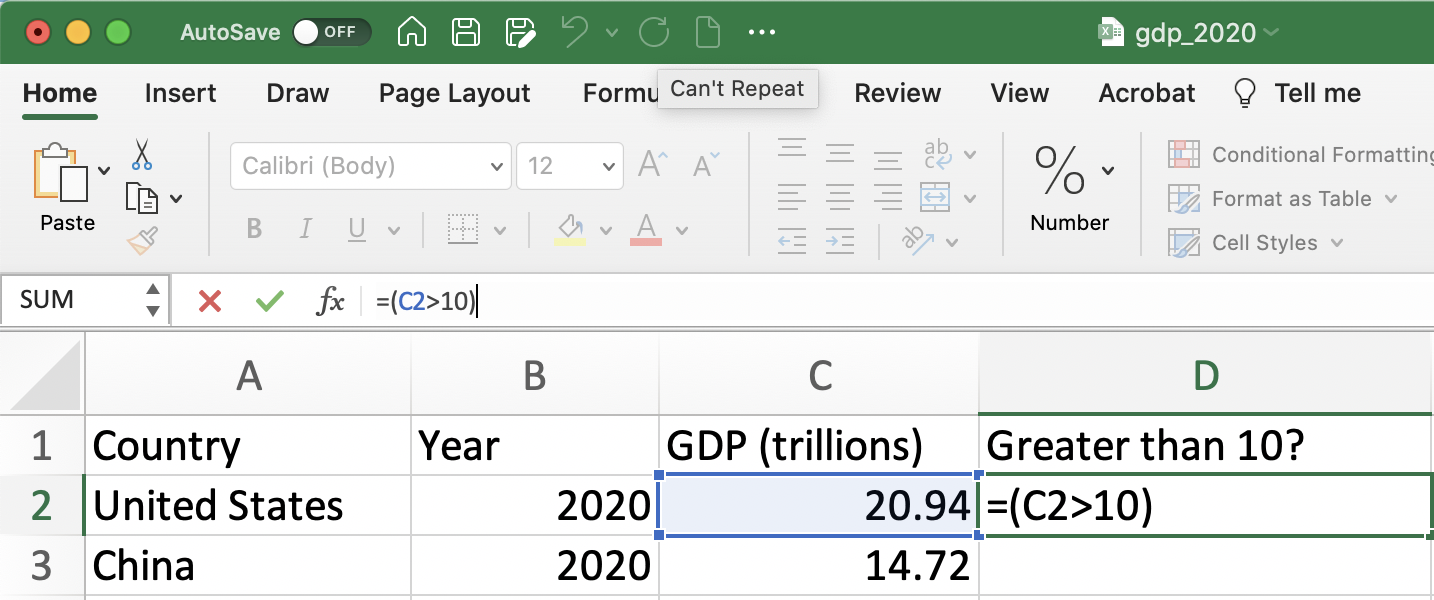
\includegraphics[width=1\linewidth]{images/01_tf1} 

}

\caption{Is GDP Greater than 10 in the U.S. Part 1}\label{fig:tf1}
\end{figure}

Once we press enter, we will get the result. In this case, we can see GDP in the U.S. is indeed greater than 10 trillion dollars. Therefore, when the function in cell D2 is evaluated it returns the answer \texttt{TRUE}, as can be seen in Figure \ref{fig:tf2}.

\begin{figure}

{\centering 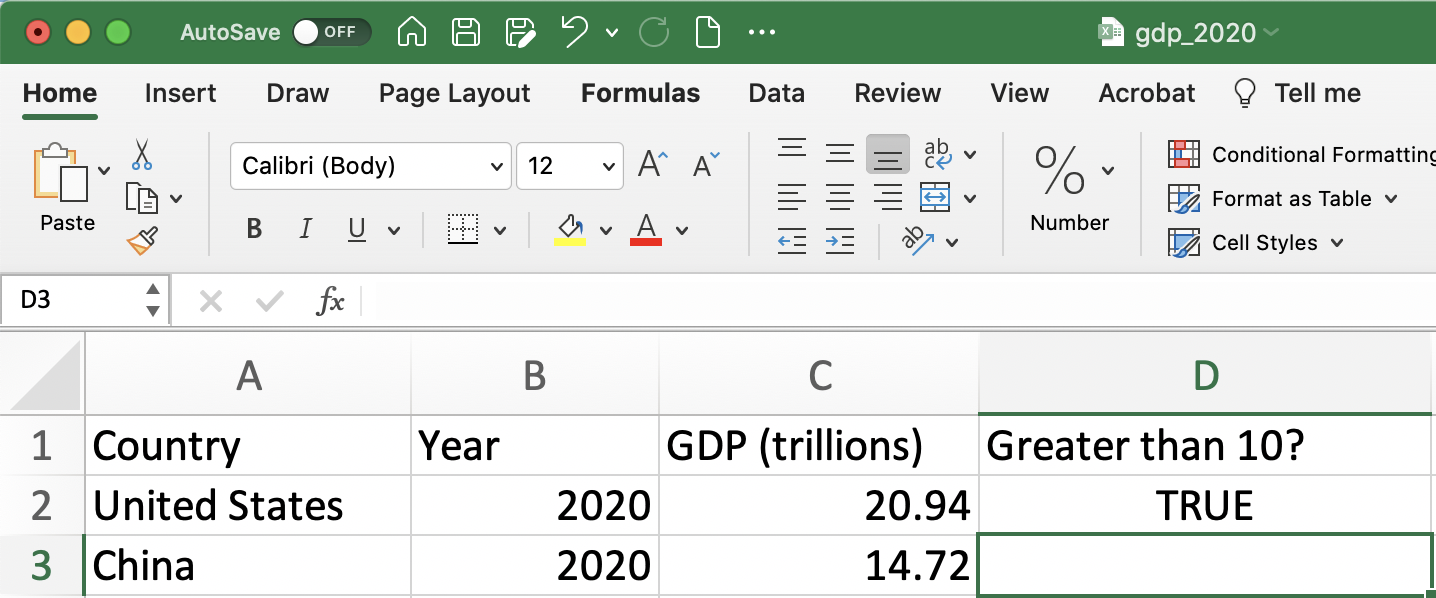
\includegraphics[width=1\linewidth]{images/01_tf2} 

}

\caption{Is GDP Greater than 10 in the U.S. Part 2}\label{fig:tf2}
\end{figure}

Once we have filled in the formula for one cell, we can also apply it to the remaining observations. In our example, this would mean testing whether each country's GDP is more than 10, not just the U.S. There are a couple of ways to do this efficiently in Excel.

One way to fill in the formula is to click the bottom right corner of cell D2 and then drag down. This allows you to apply to as many observations as you would like. However, we often want to apply the logical statement to all observations. Therefore, continuously dragging will be inefficient if there are thousands of observations in the data. To quickly apply a formula to all cells in a column, we can simply double-click the bottom right corner of a cell. In our example, this would mean double-clicking the bottom right corner of the D2 cell.

\begin{figure}

{\centering 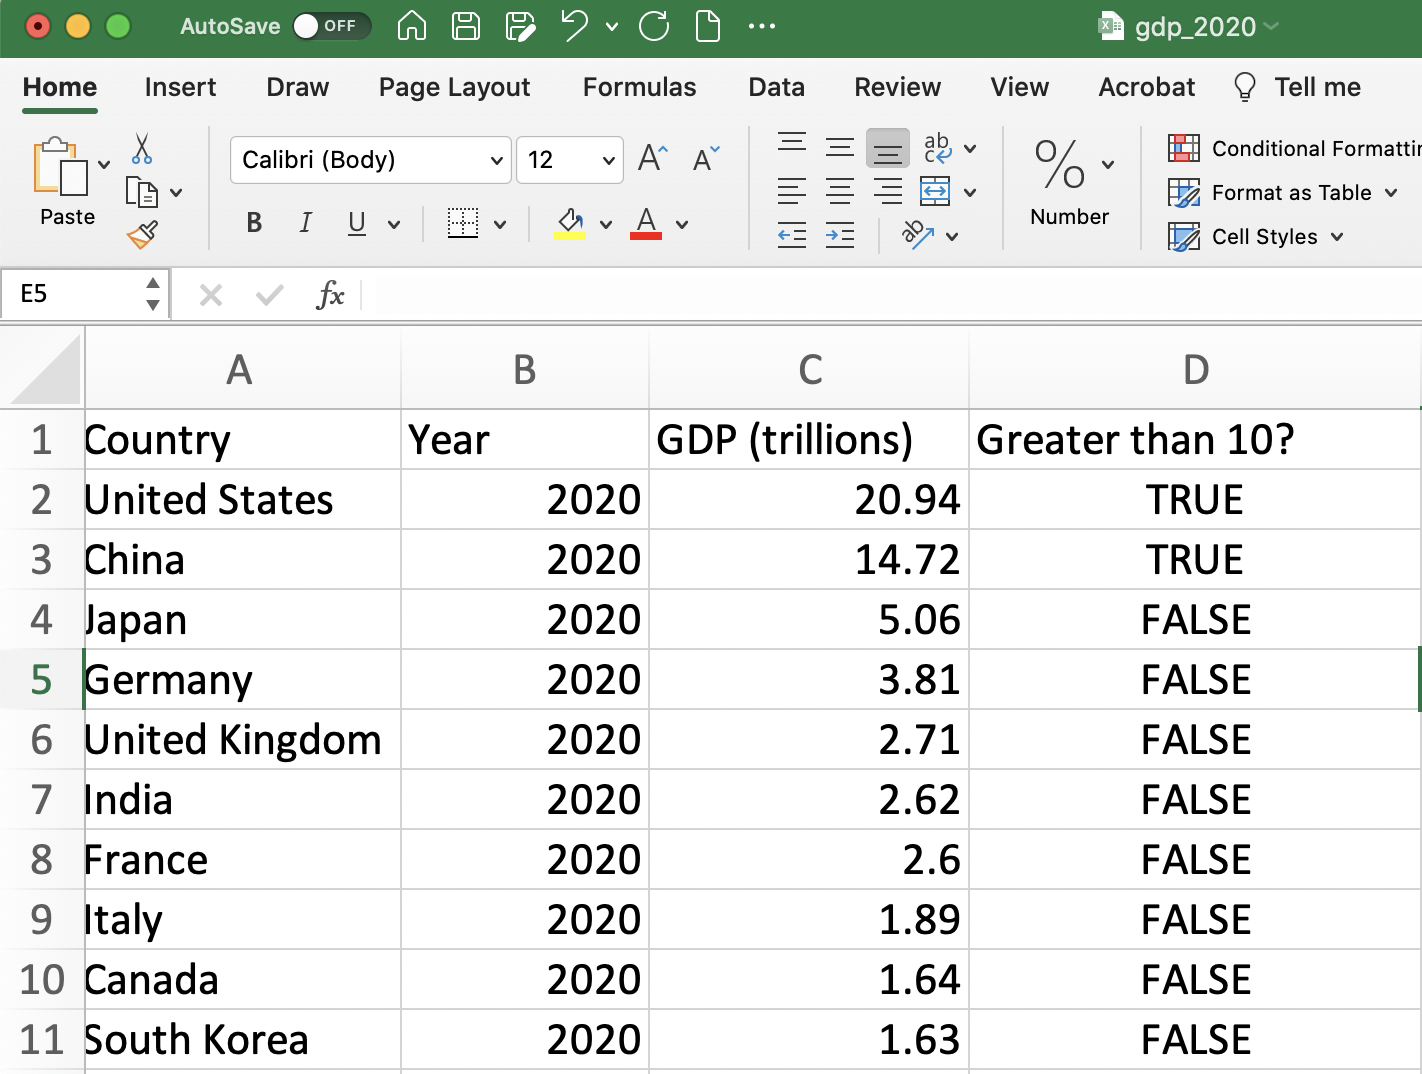
\includegraphics[width=1\linewidth]{images/01_fill} 

}

\caption{Filling in the Formula}\label{fig:fill}
\end{figure}

Oftentimes, instead of returning ``TRUE'' or ``FALSE'', it is convenient to have Excel return the value in another form. For example, a common way to represent ``TRUE'' is with the number 1 and ``FALSE'' with the number 0. To accomplish this in Excel we will use the \texttt{IF} function.

The basic format for the \texttt{IF} function is:

\texttt{=IF(logical\ test,value\ if\ TRUE,\ value\ if\ FALSE)}

For example, in our dataset, if we want to return the value of 1 if GDP is greater than 10 and 0 if otherwise, we can type:

\texttt{=IF(C2\textgreater{}10,1,0)}

\begin{figure}

{\centering 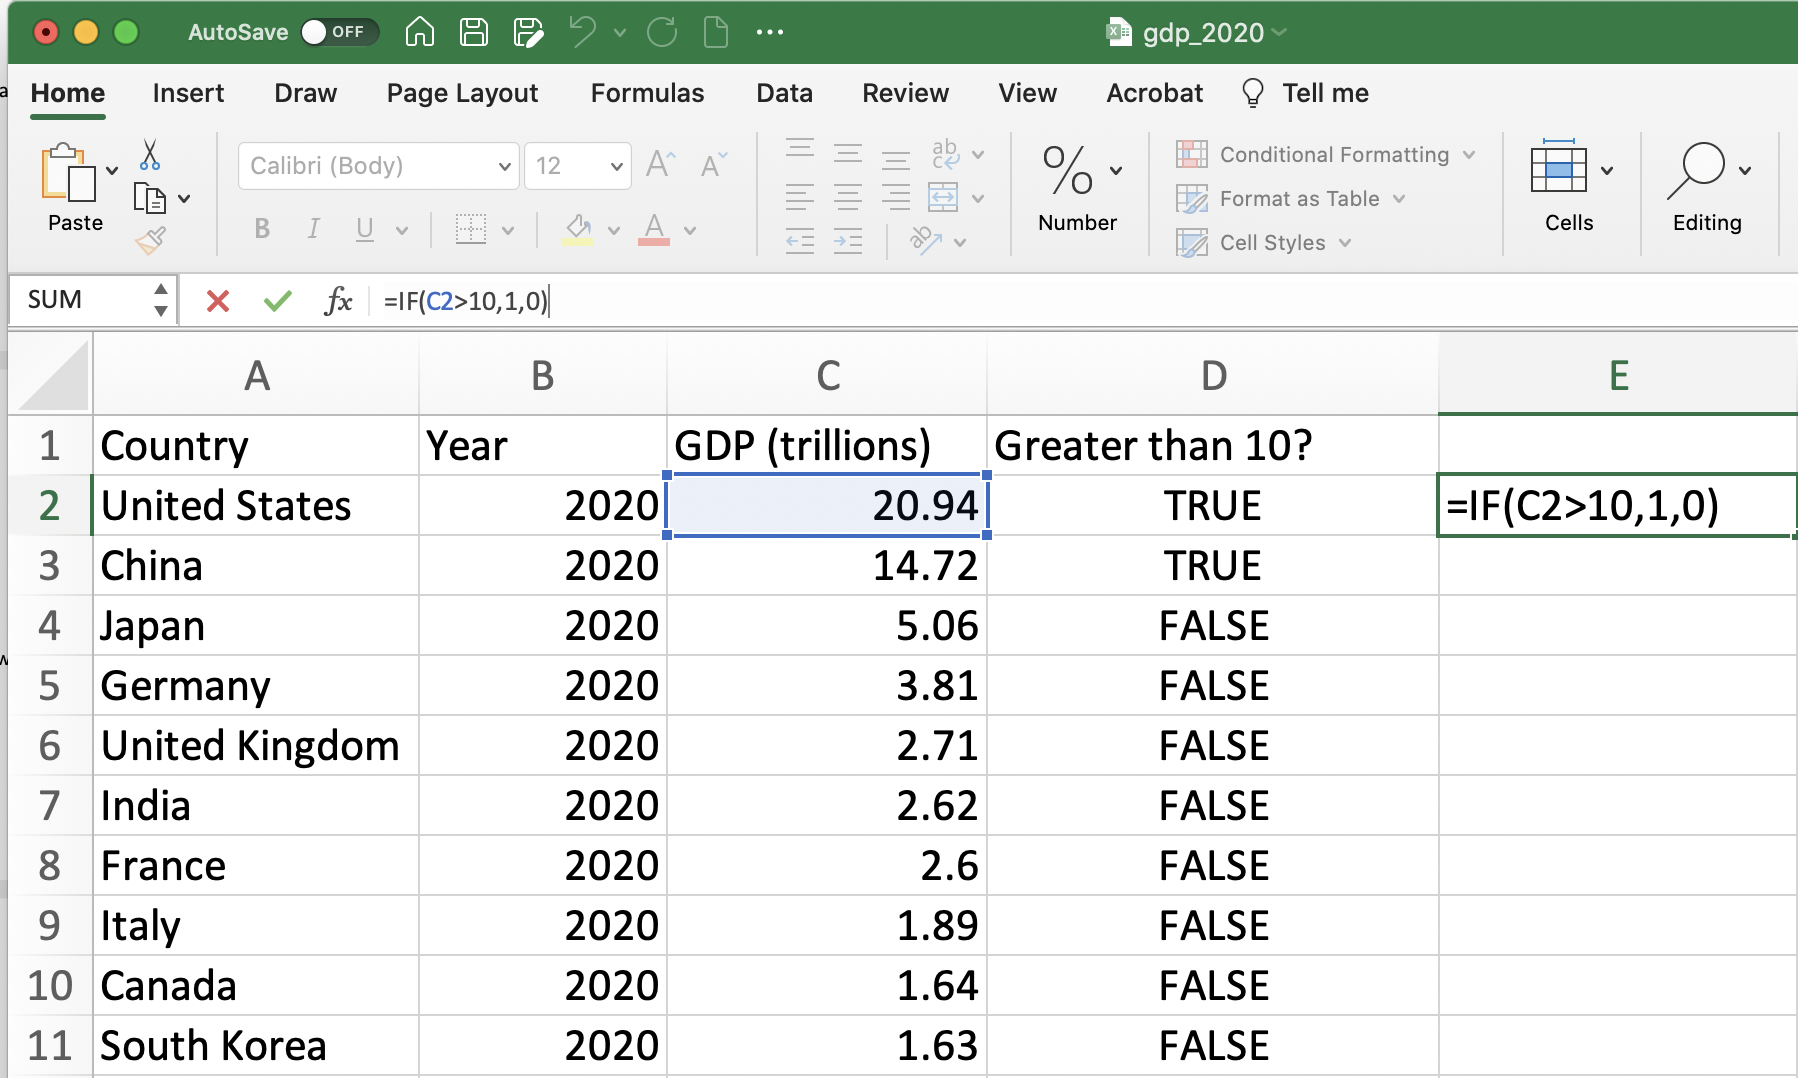
\includegraphics[width=1\linewidth]{images/01_if1} 

}

\caption{Using the IF function (Before Pressing Enter)}\label{fig:ifex1}
\end{figure}

Once we press enter, the function is evaluated. To fill in the formula for the rest of the observations you can follow the same steps as above.

\begin{figure}

{\centering 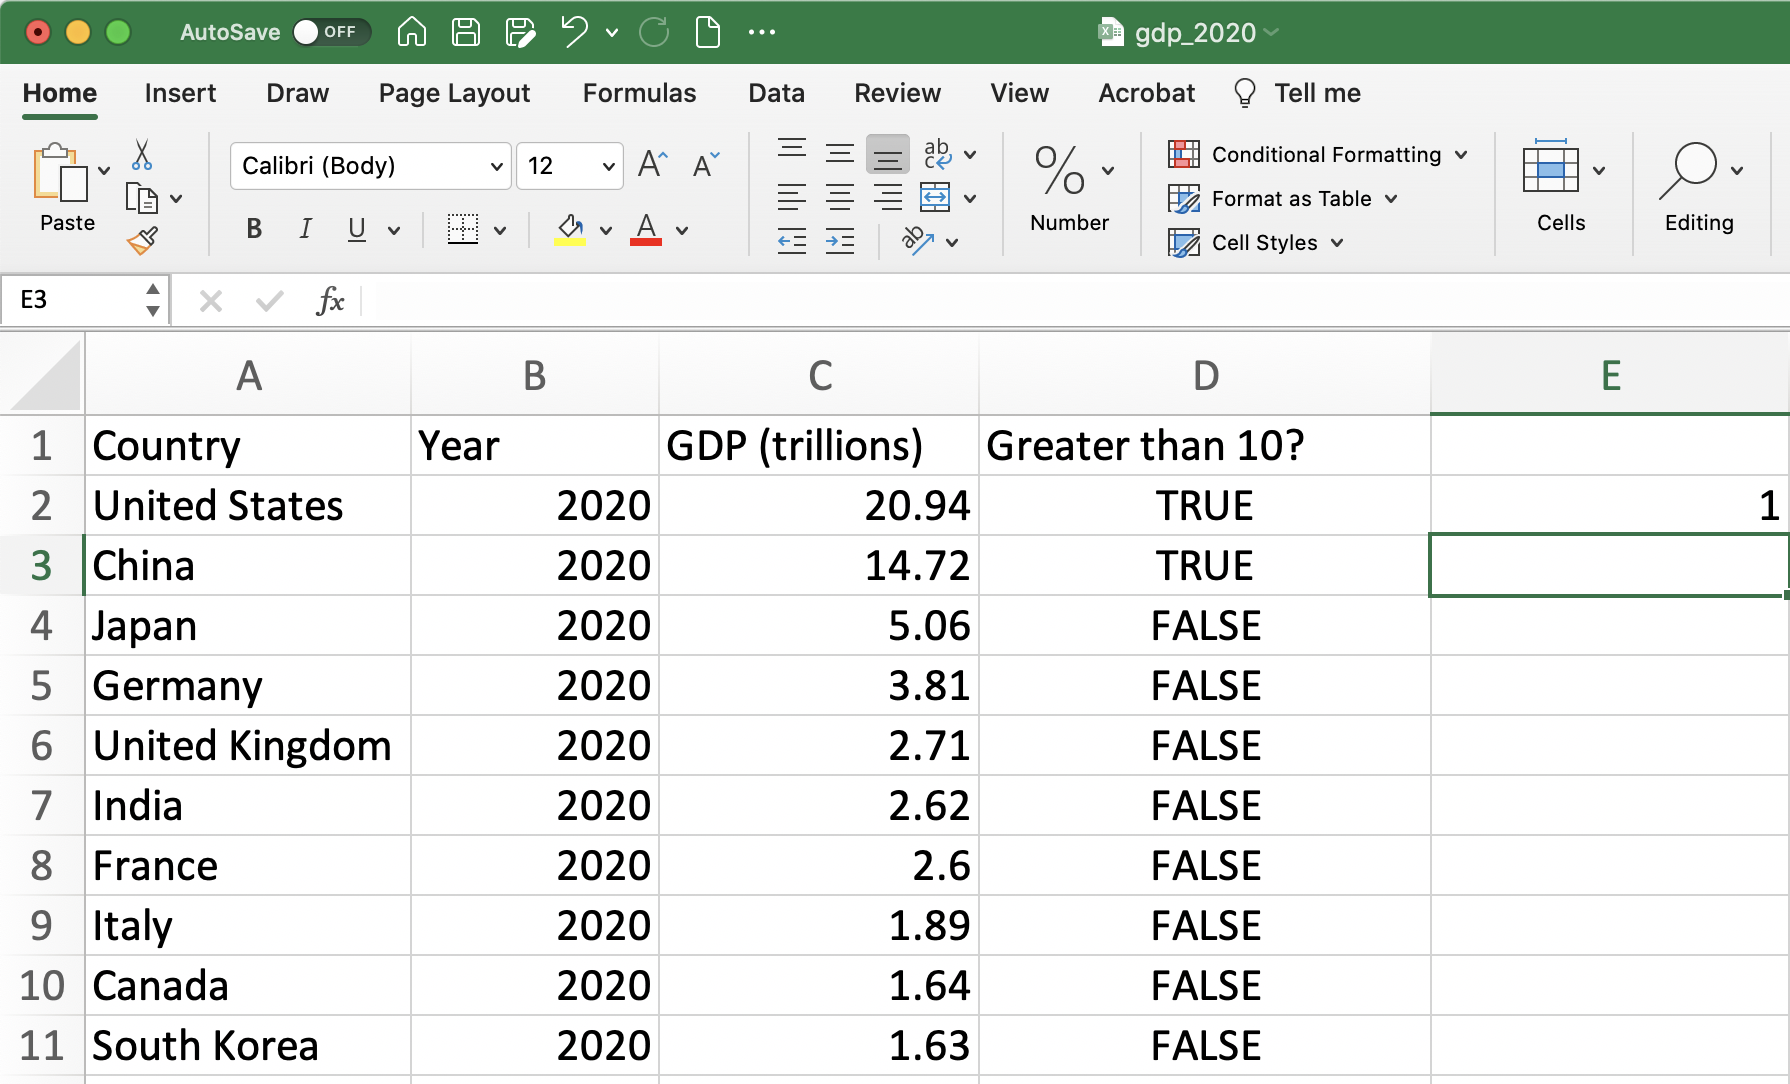
\includegraphics[width=1\linewidth]{images/01_if2} 

}

\caption{Using the IF function (After Pressing Enter)}\label{fig:ifex2}
\end{figure}

\section{Summary Statistics}\label{summary-statistics}

Now let's return to our data from Brownback and Sadoff (2020). Our goal is to create a table of basic summary statistics. However, a key variable in the Brownback and Sadoff (2020) experiment is whether a given student passed the test or not. In this setting, a score of 70 or higher indicates that the student passed the test. Therefore we need to create a new variable that is equal to 1 if the individual received a \texttt{TestScore} greater than or equal to 70 and zero otherwise. We will show later that storing this information as a 1 or zero will be particularly convenient for our analysis.

To create this variable we need to take three steps:

\begin{itemize}
\item
  \textbf{First Step:} Title the column with the variable name ``Passed''
\item
  \textbf{Second Step:} Use the \texttt{IF} function to fill in this variable for the first observation
\item
  \textbf{Third Step:} Double click the bottom right of the cell in step 2 to fill in the variable for all observations
\end{itemize}

Figure \ref{fig:passed1} presents steps 1 and 2 in Excel.

\begin{figure}

{\centering 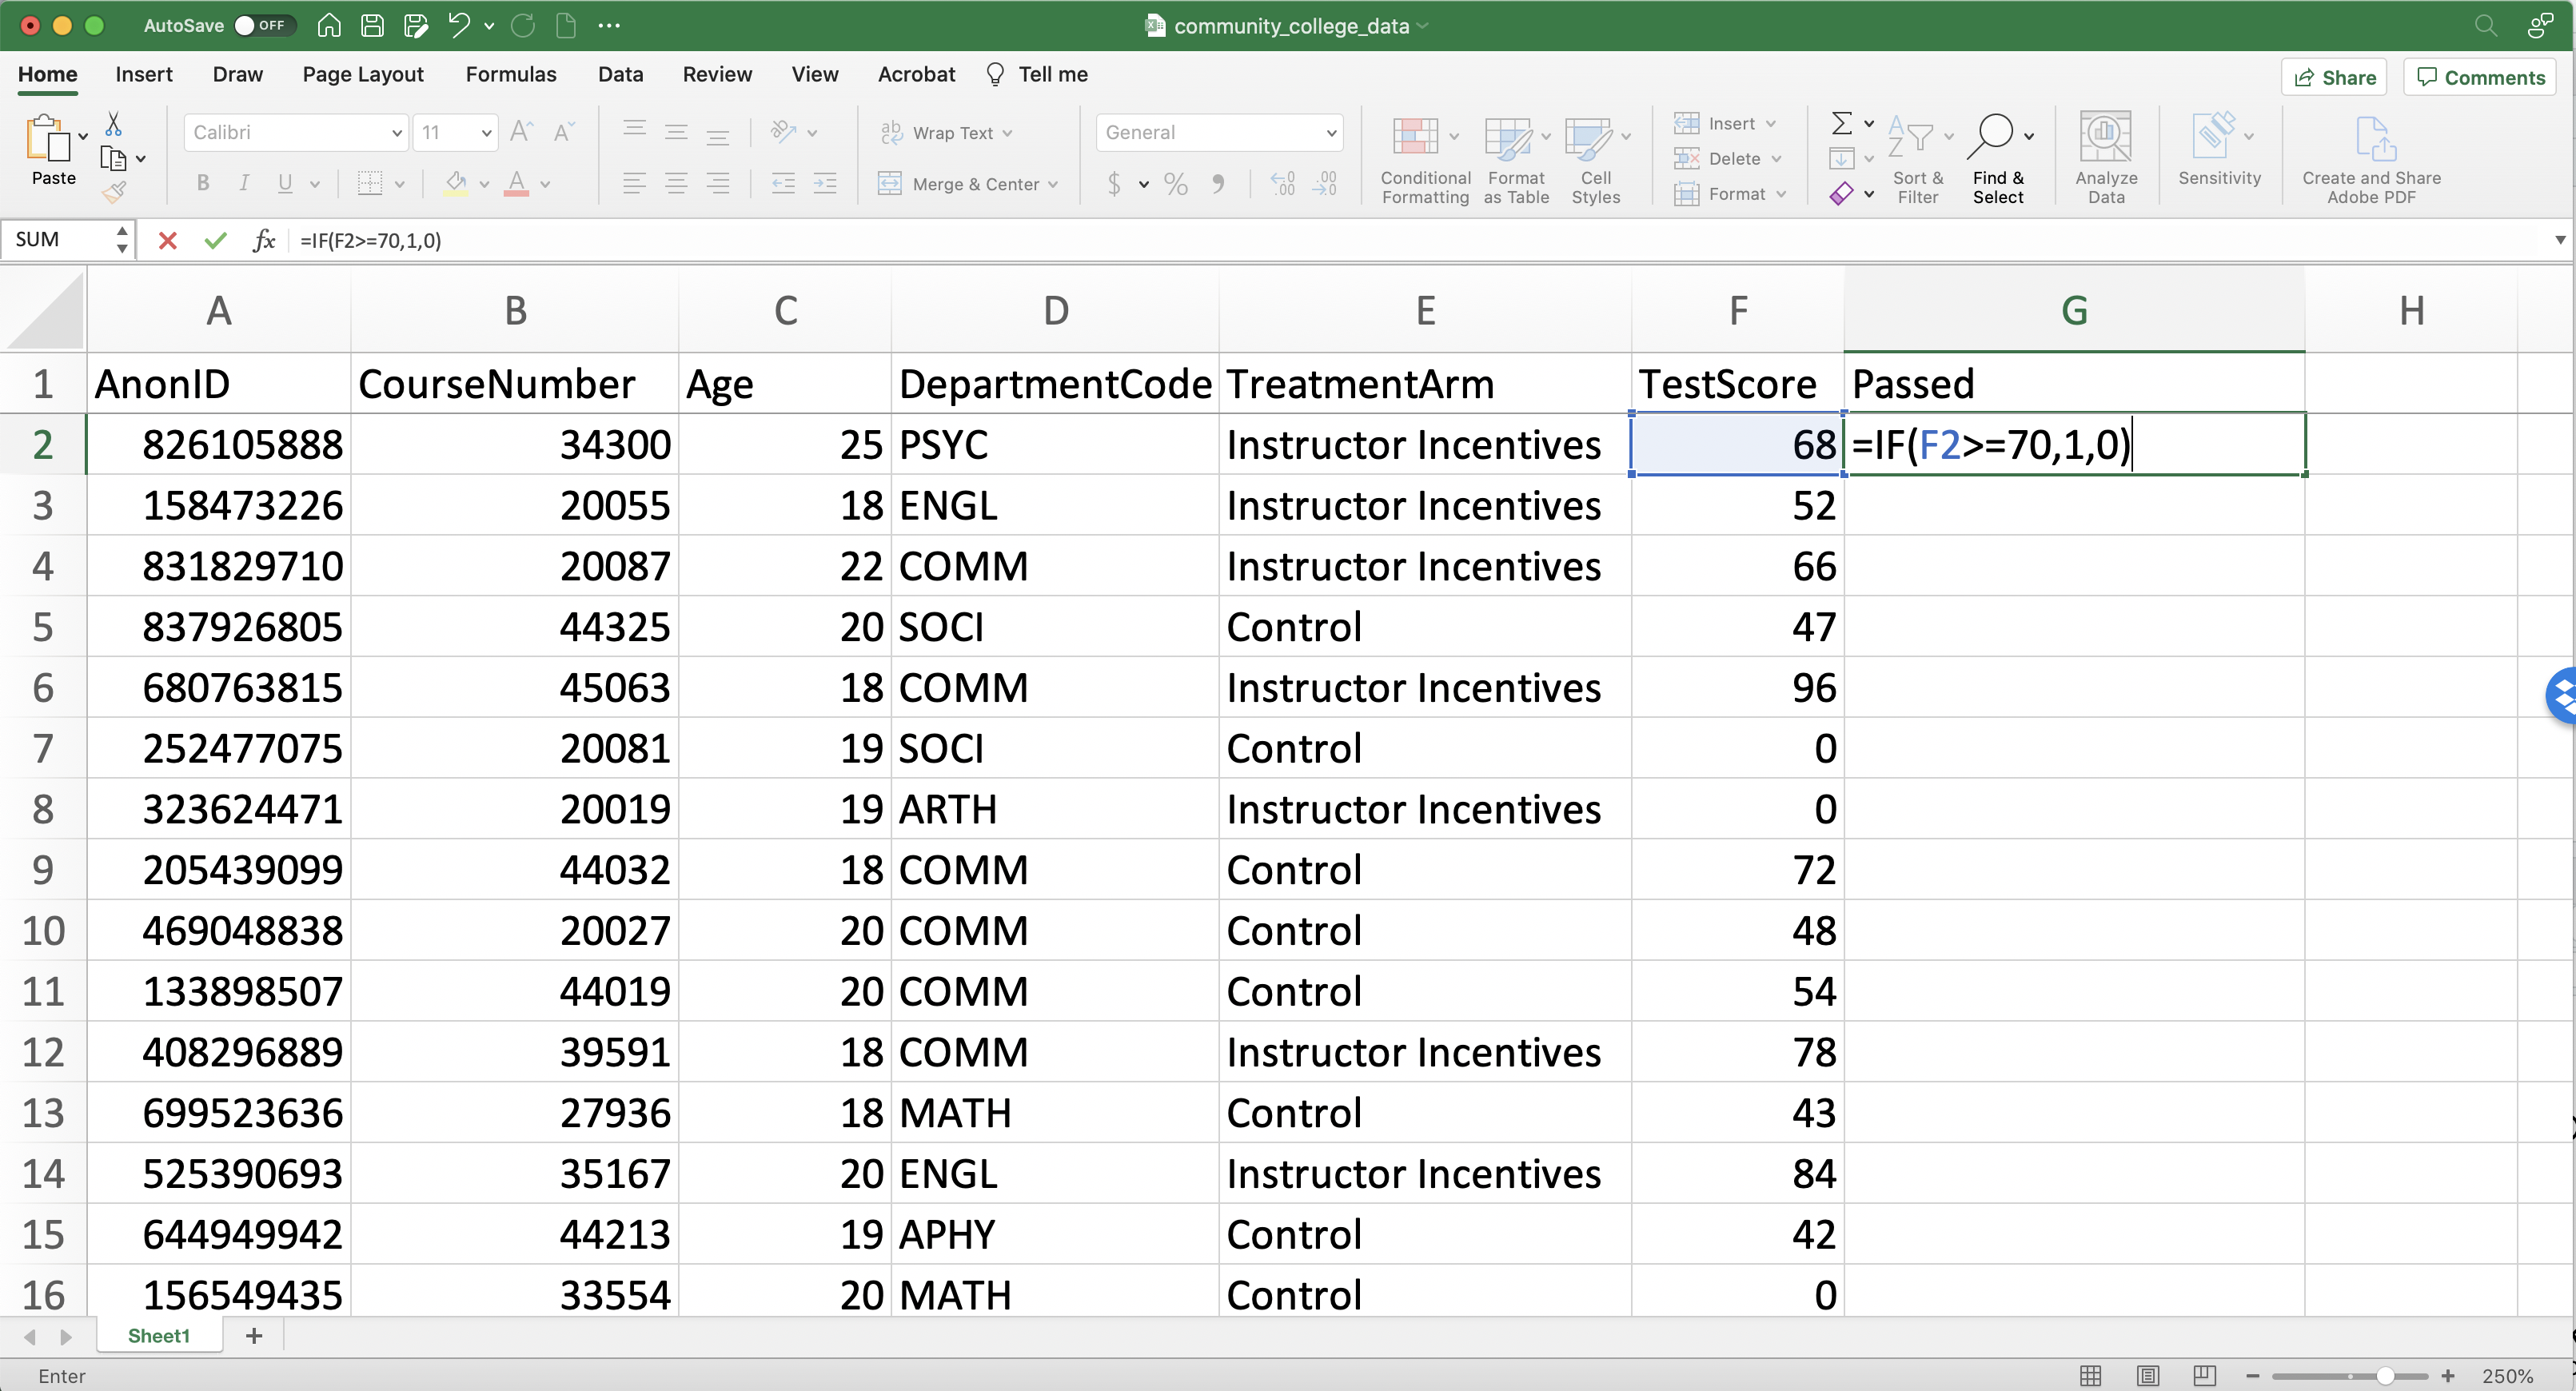
\includegraphics[width=1\linewidth]{images/01_passed1} 

}

\caption{Generating a Passed Variable (Steps 1 and 2)}\label{fig:passed1}
\end{figure}

We simply can double-click the bottom right of G2 to fill in the rest of the observations (as seen in Figure \ref{fig:passed2}).

\begin{figure}

{\centering 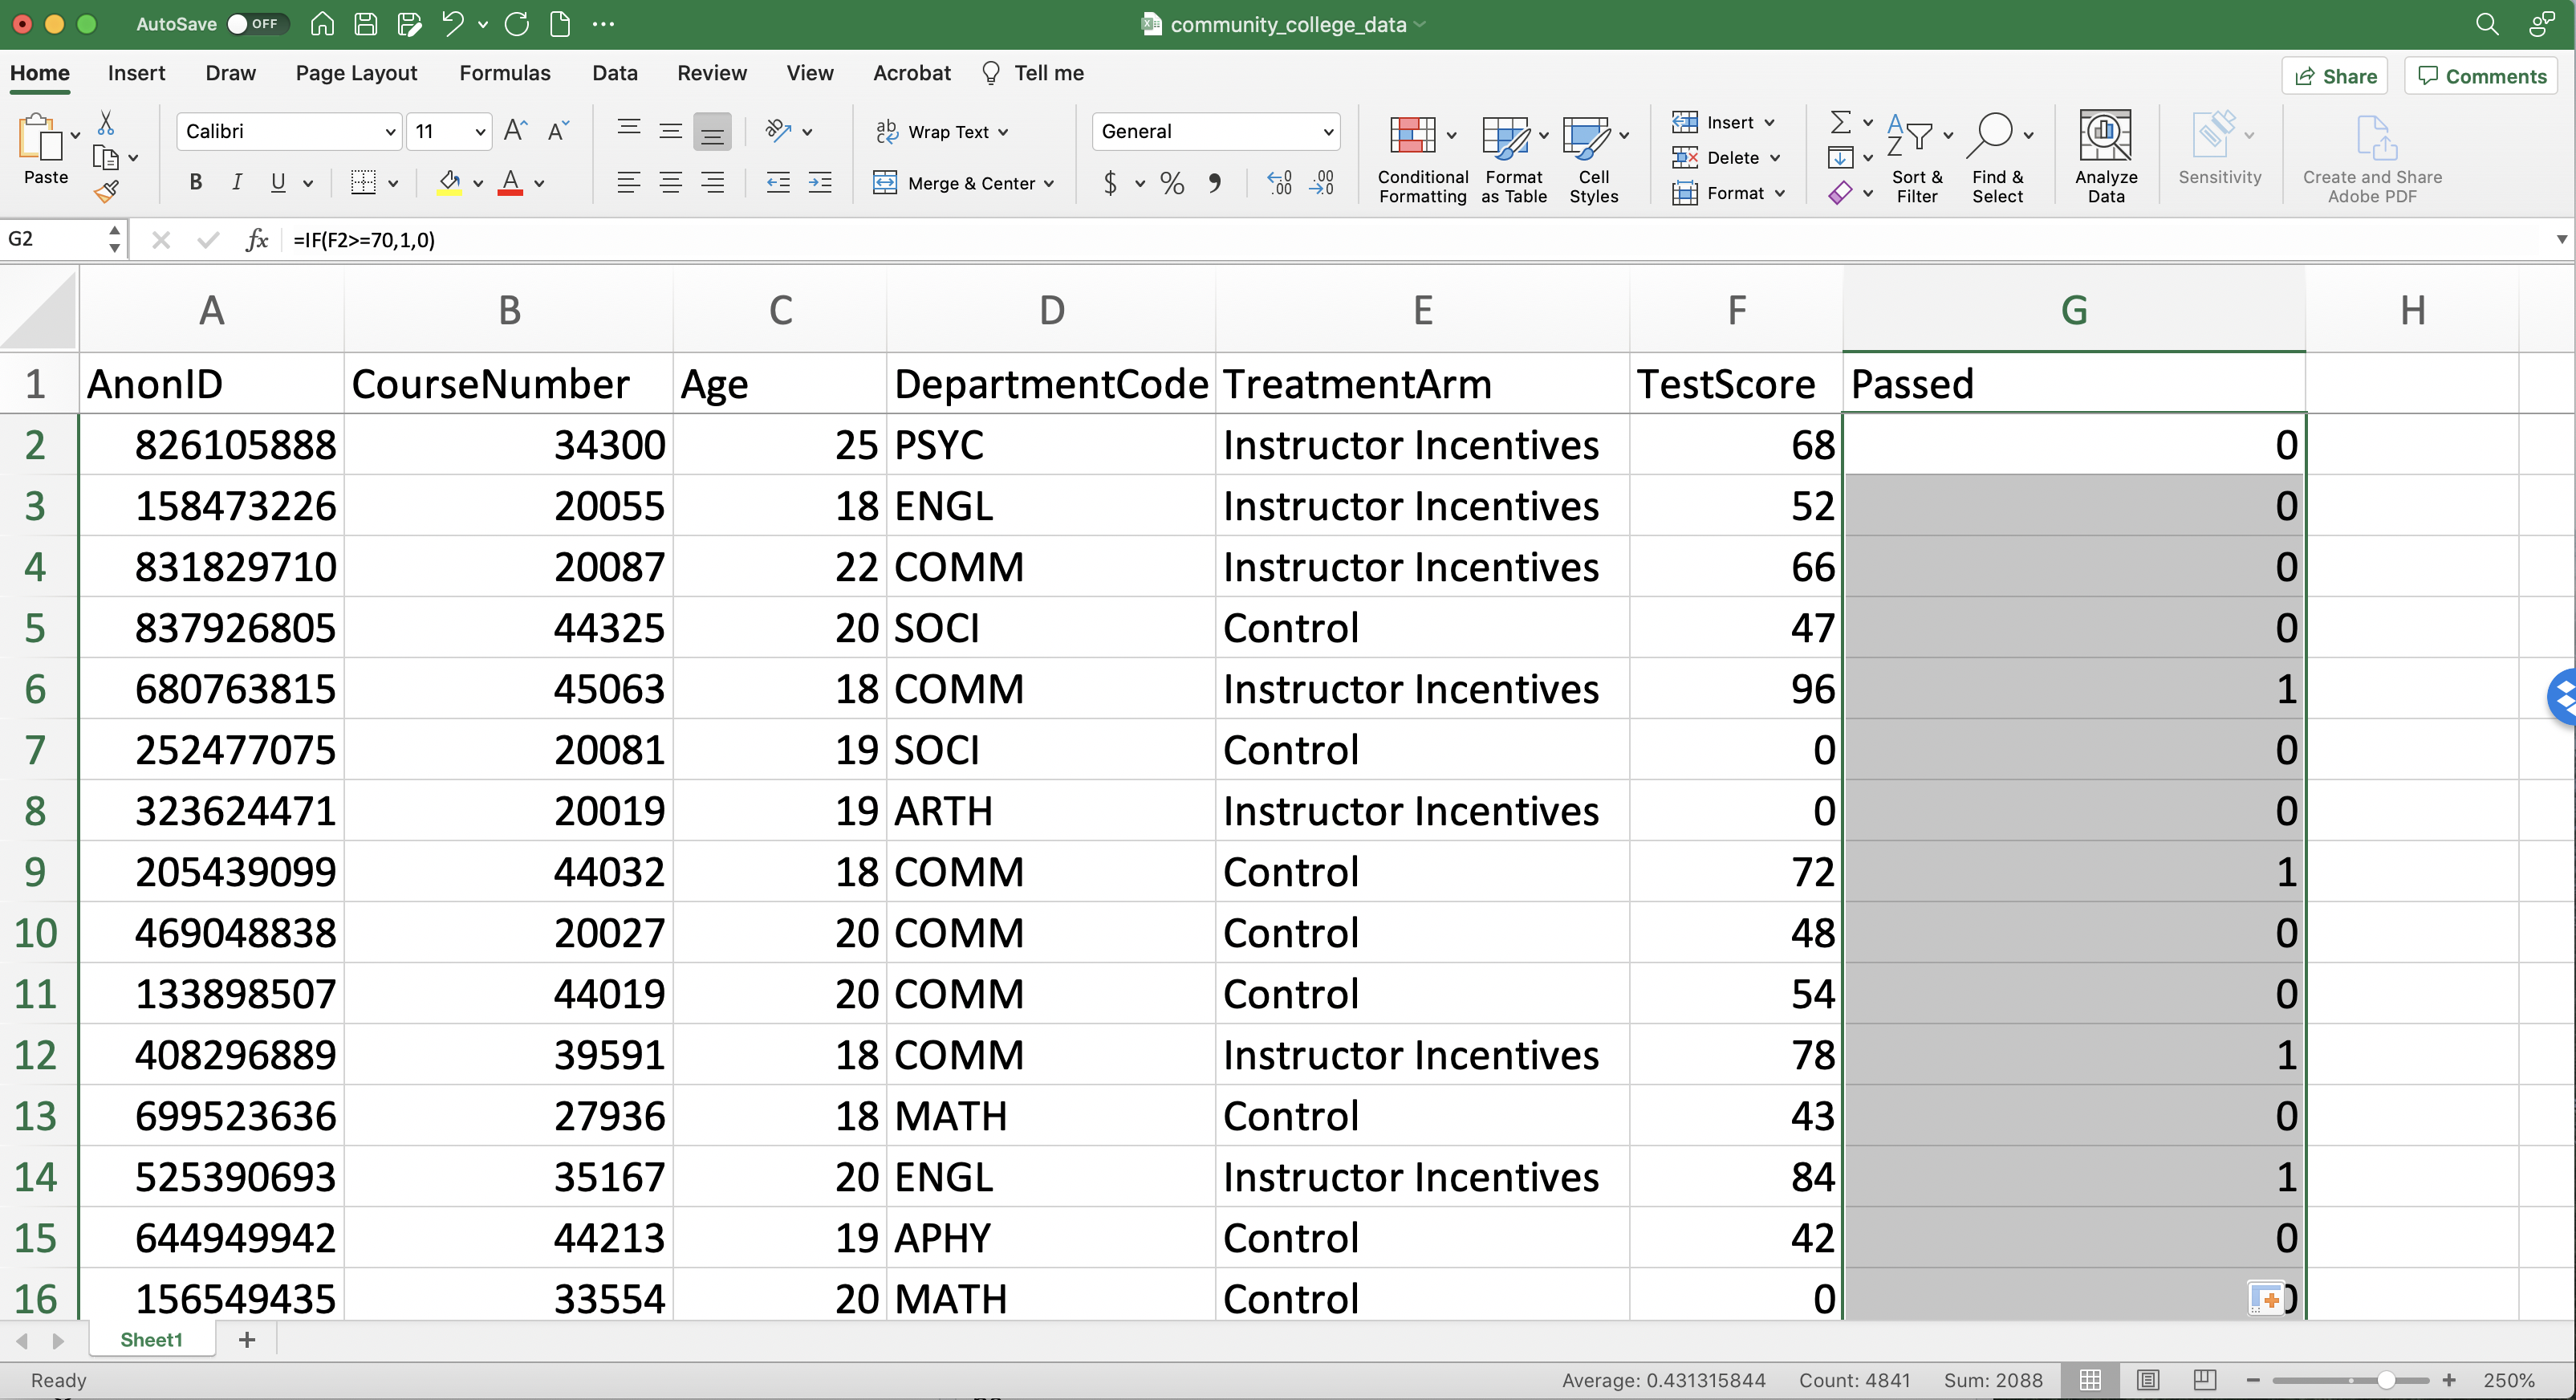
\includegraphics[width=1\linewidth]{images/01_passed2} 

}

\caption{Generating a Passed Variable (Step 3)}\label{fig:passed2}
\end{figure}

Now that we've generated the variables we need let's fill in some summary statistics displayed on the right side of the datasheet in Figure \ref{fig:sumstats1}

\begin{figure}

{\centering 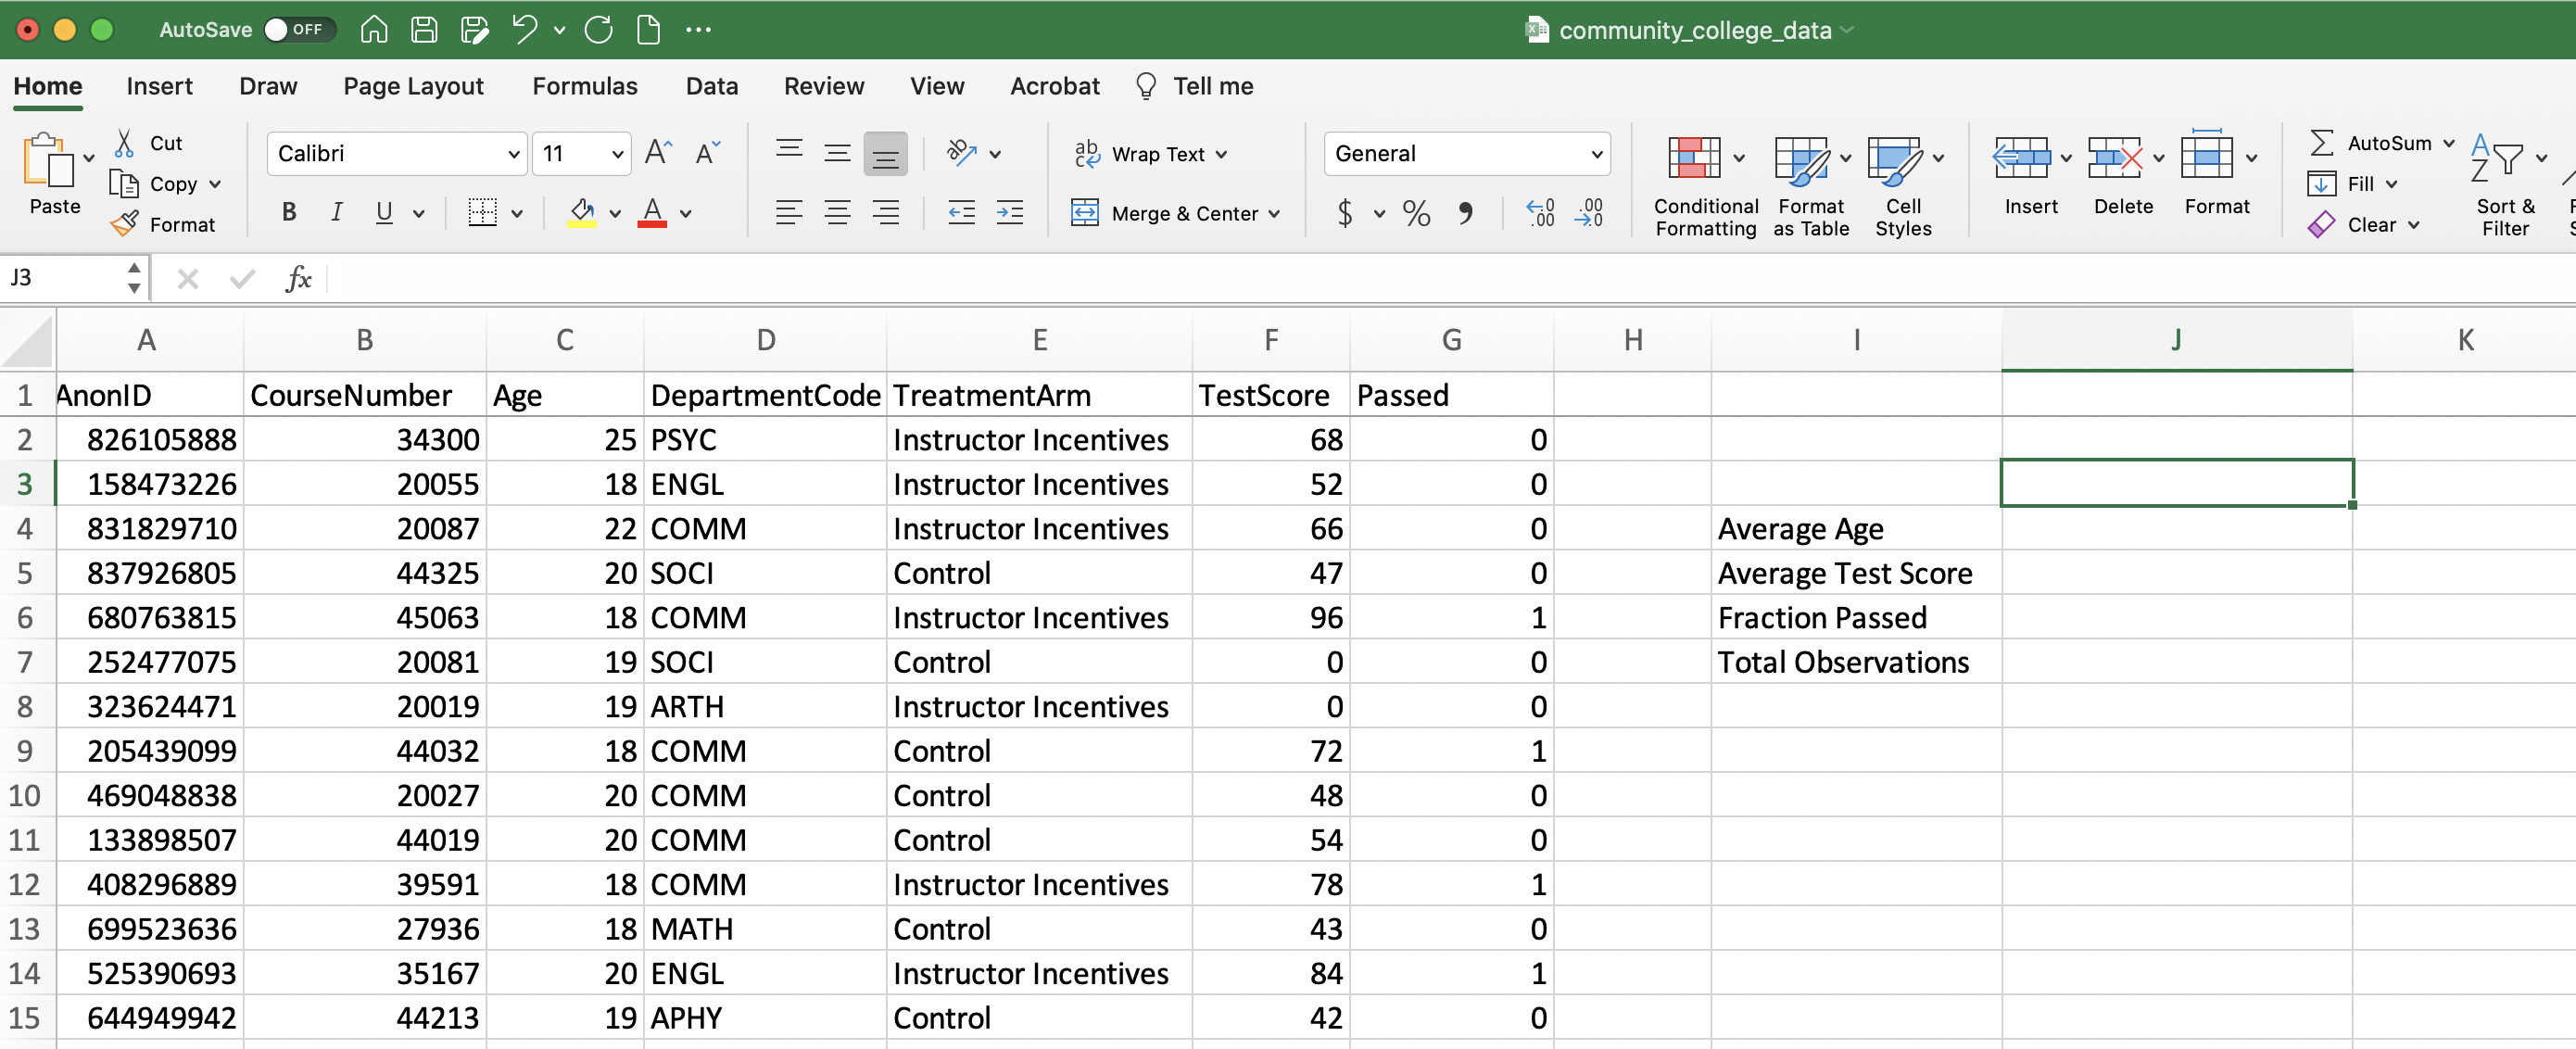
\includegraphics[width=1\linewidth]{images/01_sumstats1} 

}

\caption{Blank Summary Statistics Table}\label{fig:sumstats1}
\end{figure}

To compute the average age in the dataset we just need to use the \texttt{AVERAGE} function and reference column C.

\begin{figure}

{\centering 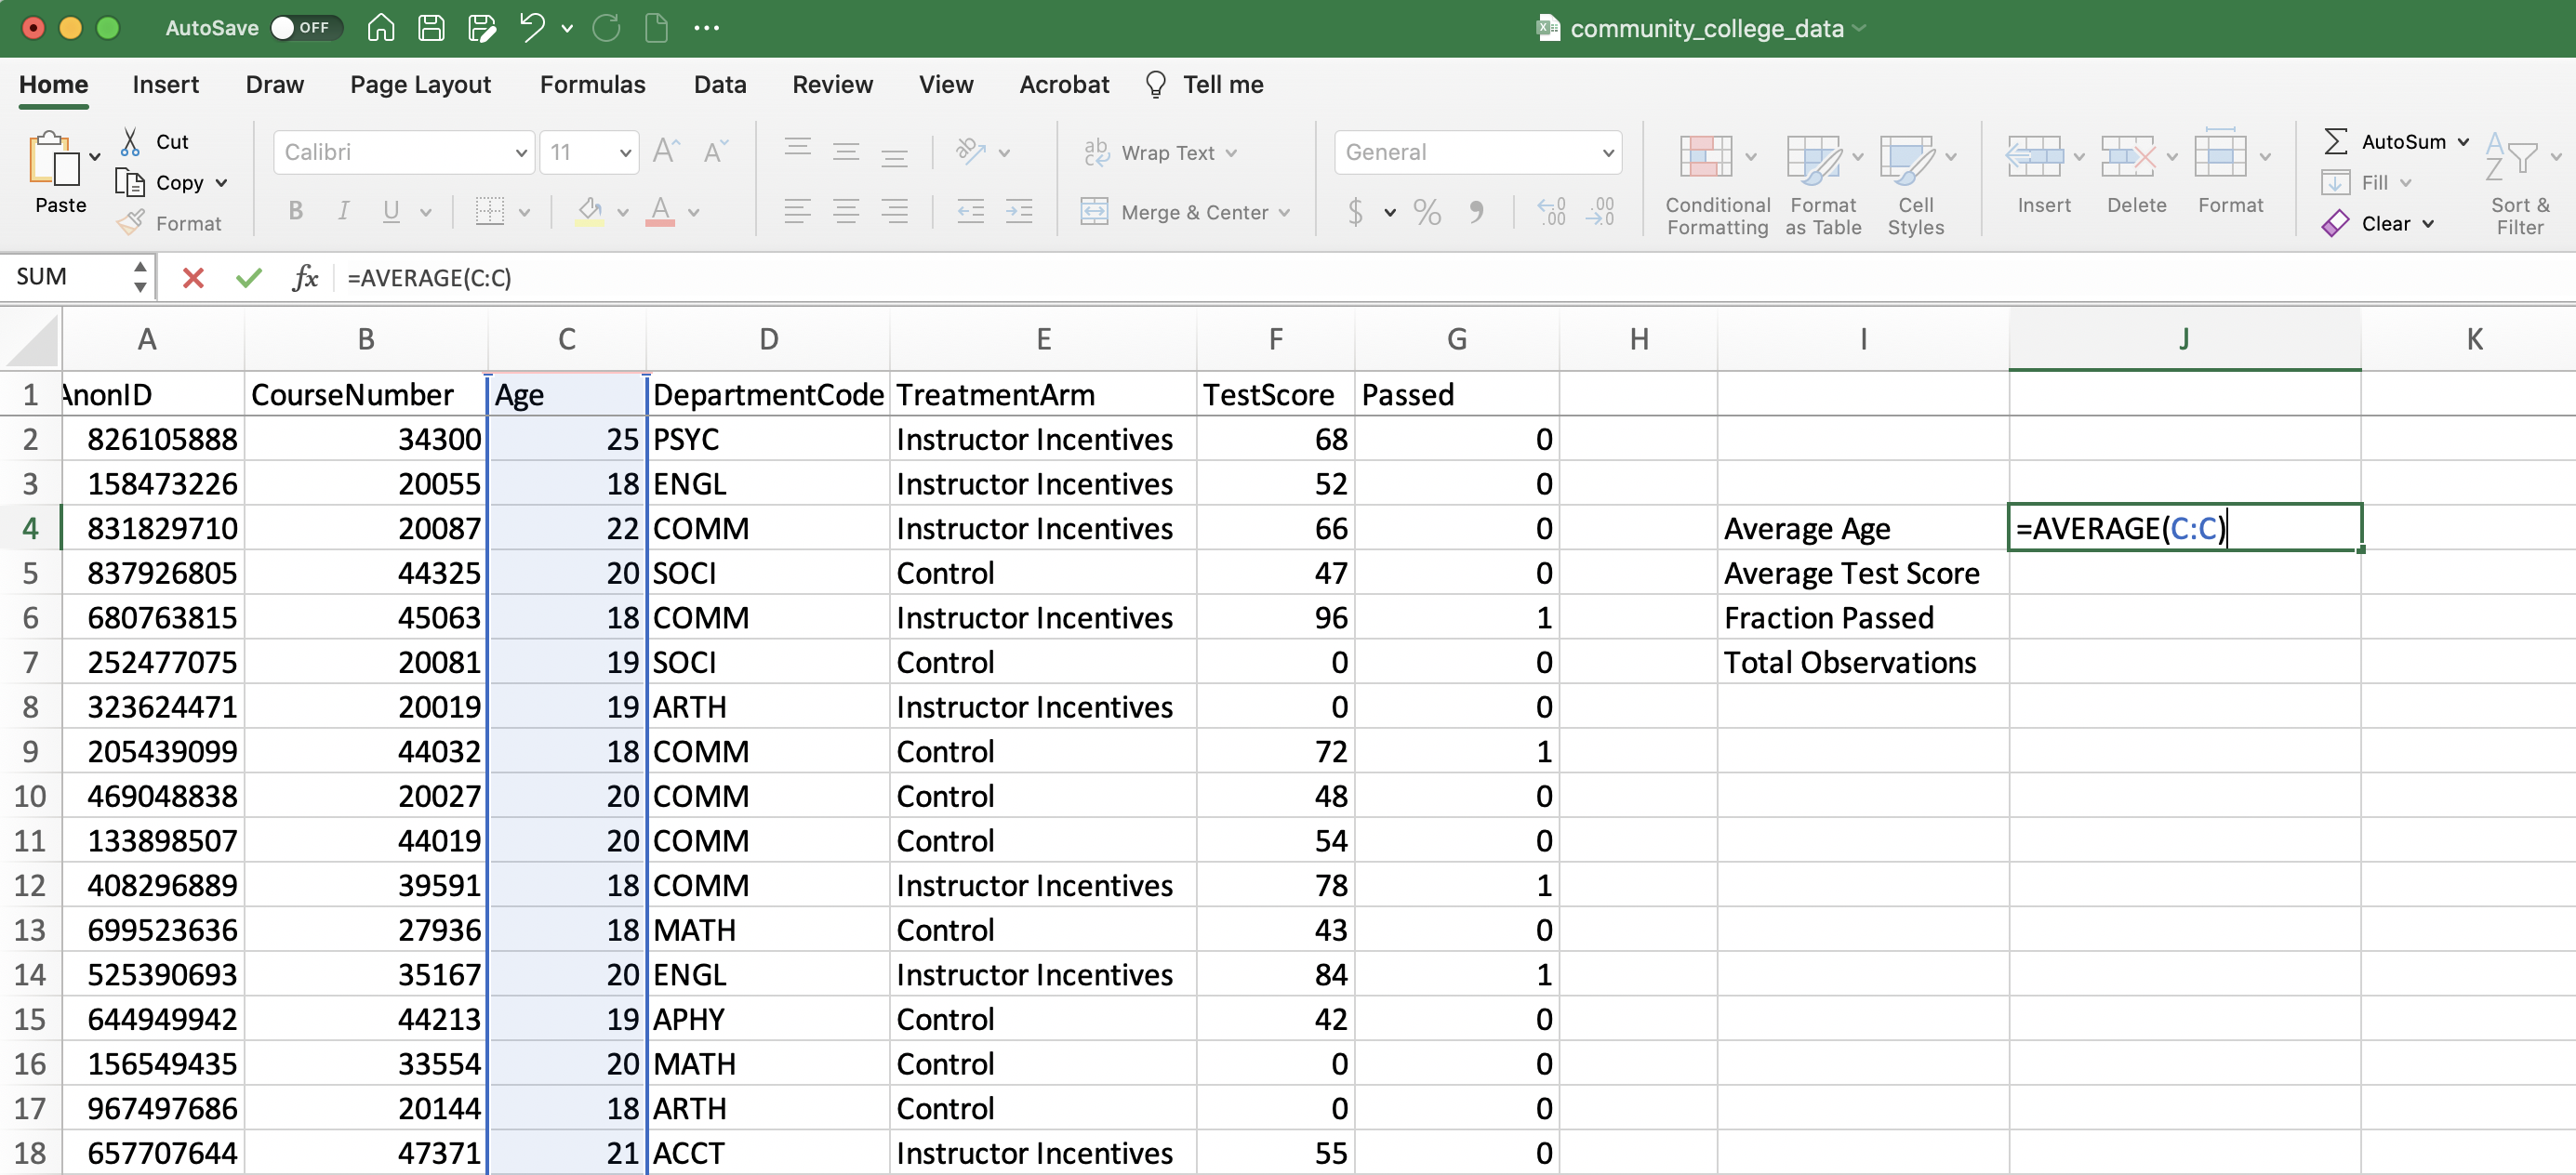
\includegraphics[width=1\linewidth]{images/01_sumstats2} 

}

\caption{Average Age}\label{fig:sumstats2}
\end{figure}

Average test score is completely analogous to age, but we now reference column F.

\begin{figure}

{\centering 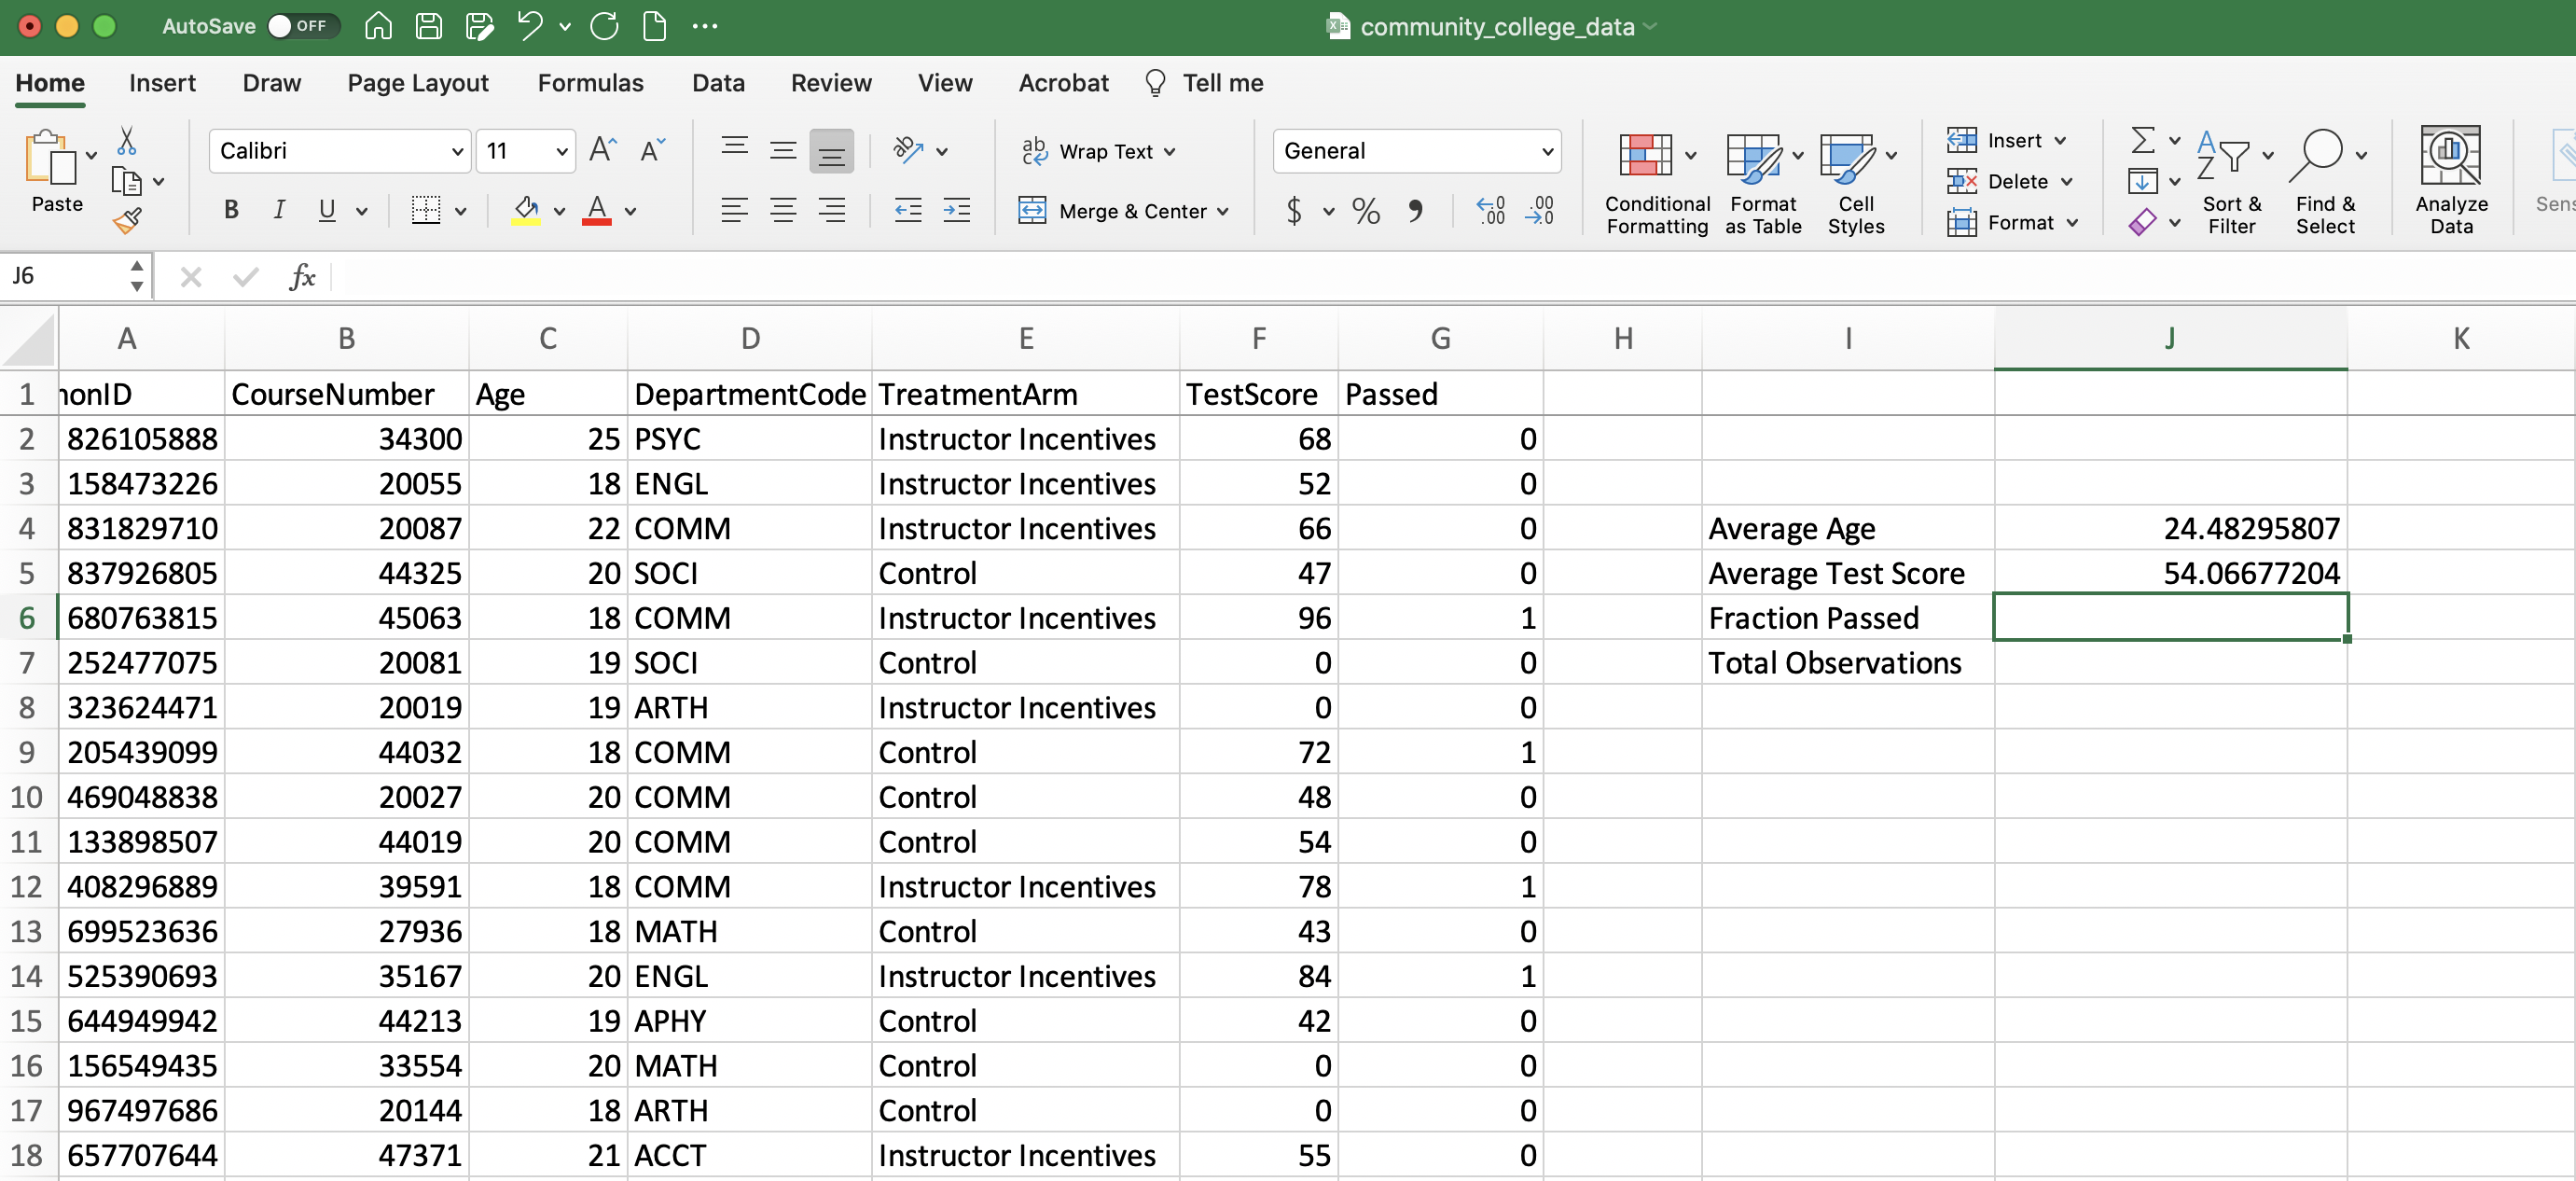
\includegraphics[width=1\linewidth]{images/01_sumstats3} 

}

\caption{Average Test Score}\label{fig:sumstats3}
\end{figure}

To compute the fraction that passed the test, we are first going to make a small digression, one that will clarify one reason it was convenient to store the variable Passed with a 1 if the individual passed and a zero otherwise. Because we have stored the variable in this way, we can simply take the average value of \texttt{Passed} and this will be equal to the fraction that passed the test.

To see why this is true, let's first write out the equation for the average of a generic variable \(X\):

\[
  \bar{X} = \frac{X_1 + ... + X_N}{N} 
\]

Where \(\bar{X}\) is the average, \(N\) is the number of observations, \(X_1\) is the first observation and \(X_N\) is the \(N^{th}\) observation. If \(X\) is a binary variable that is equal to 1 or zero, then the average will be the fraction of individuals with a 1
\[
  \bar{X} = \frac{X_1 + ... + X_N}{N}=\frac{\text{Number of observations =1 }}{\text{Total Observations}} 
\]
Since our variable ``Passed'' is equal to 1 if passed and zero otherwise, the fraction who passed is the average of our ``Passed'' variable. Therefore, in Excel we simply need to compute the average of the G column

\begin{figure}

{\centering 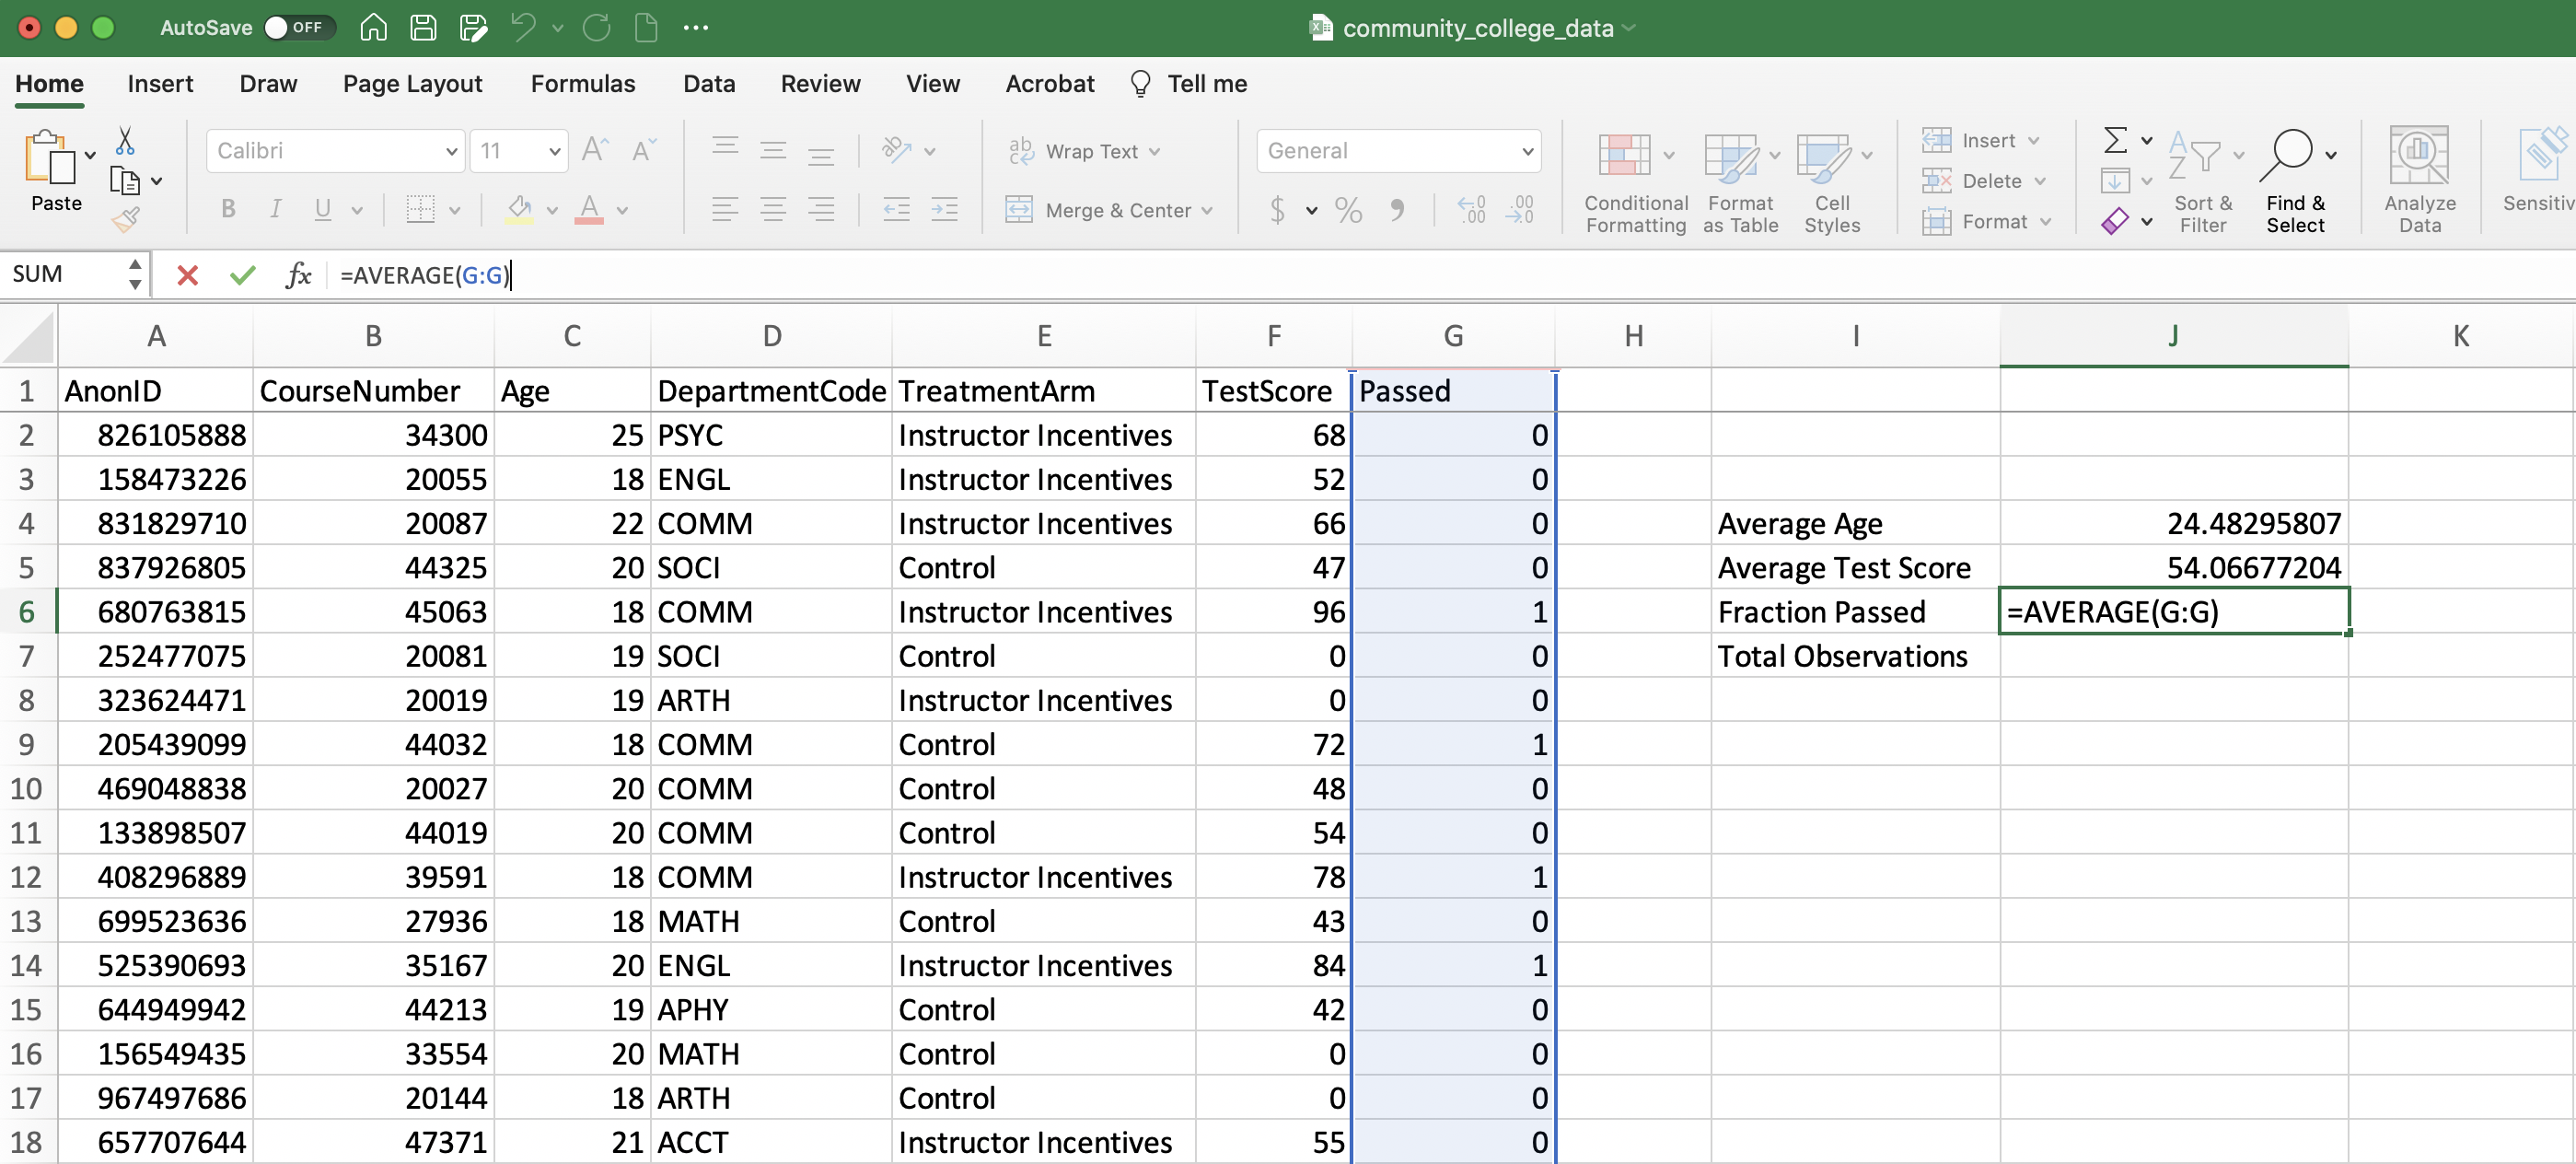
\includegraphics[width=1\linewidth]{images/01_frac_passed} 

}

\caption{Computing the Fraction Passed}\label{fig:fracpassed}
\end{figure}

We will take a lot of averages of binary variables in this book. It will be beneficial down the road to convince yourself that the average of \texttt{Passed} is equal to the fraction that passed. If you are still confused about this concept, try to convince yourself in datatsets with only a few observations why this fact is true.

Finally, to finish our summary statistics table, we need to fill in the total number of observations. To do this, we can use the \texttt{COUNT} function, which will count the total number of numbers in a column. While Figure \ref{fig:count} uses Column G to compute total observations, this could be replaced with any column that has non-missing numeric data.

\begin{figure}

{\centering 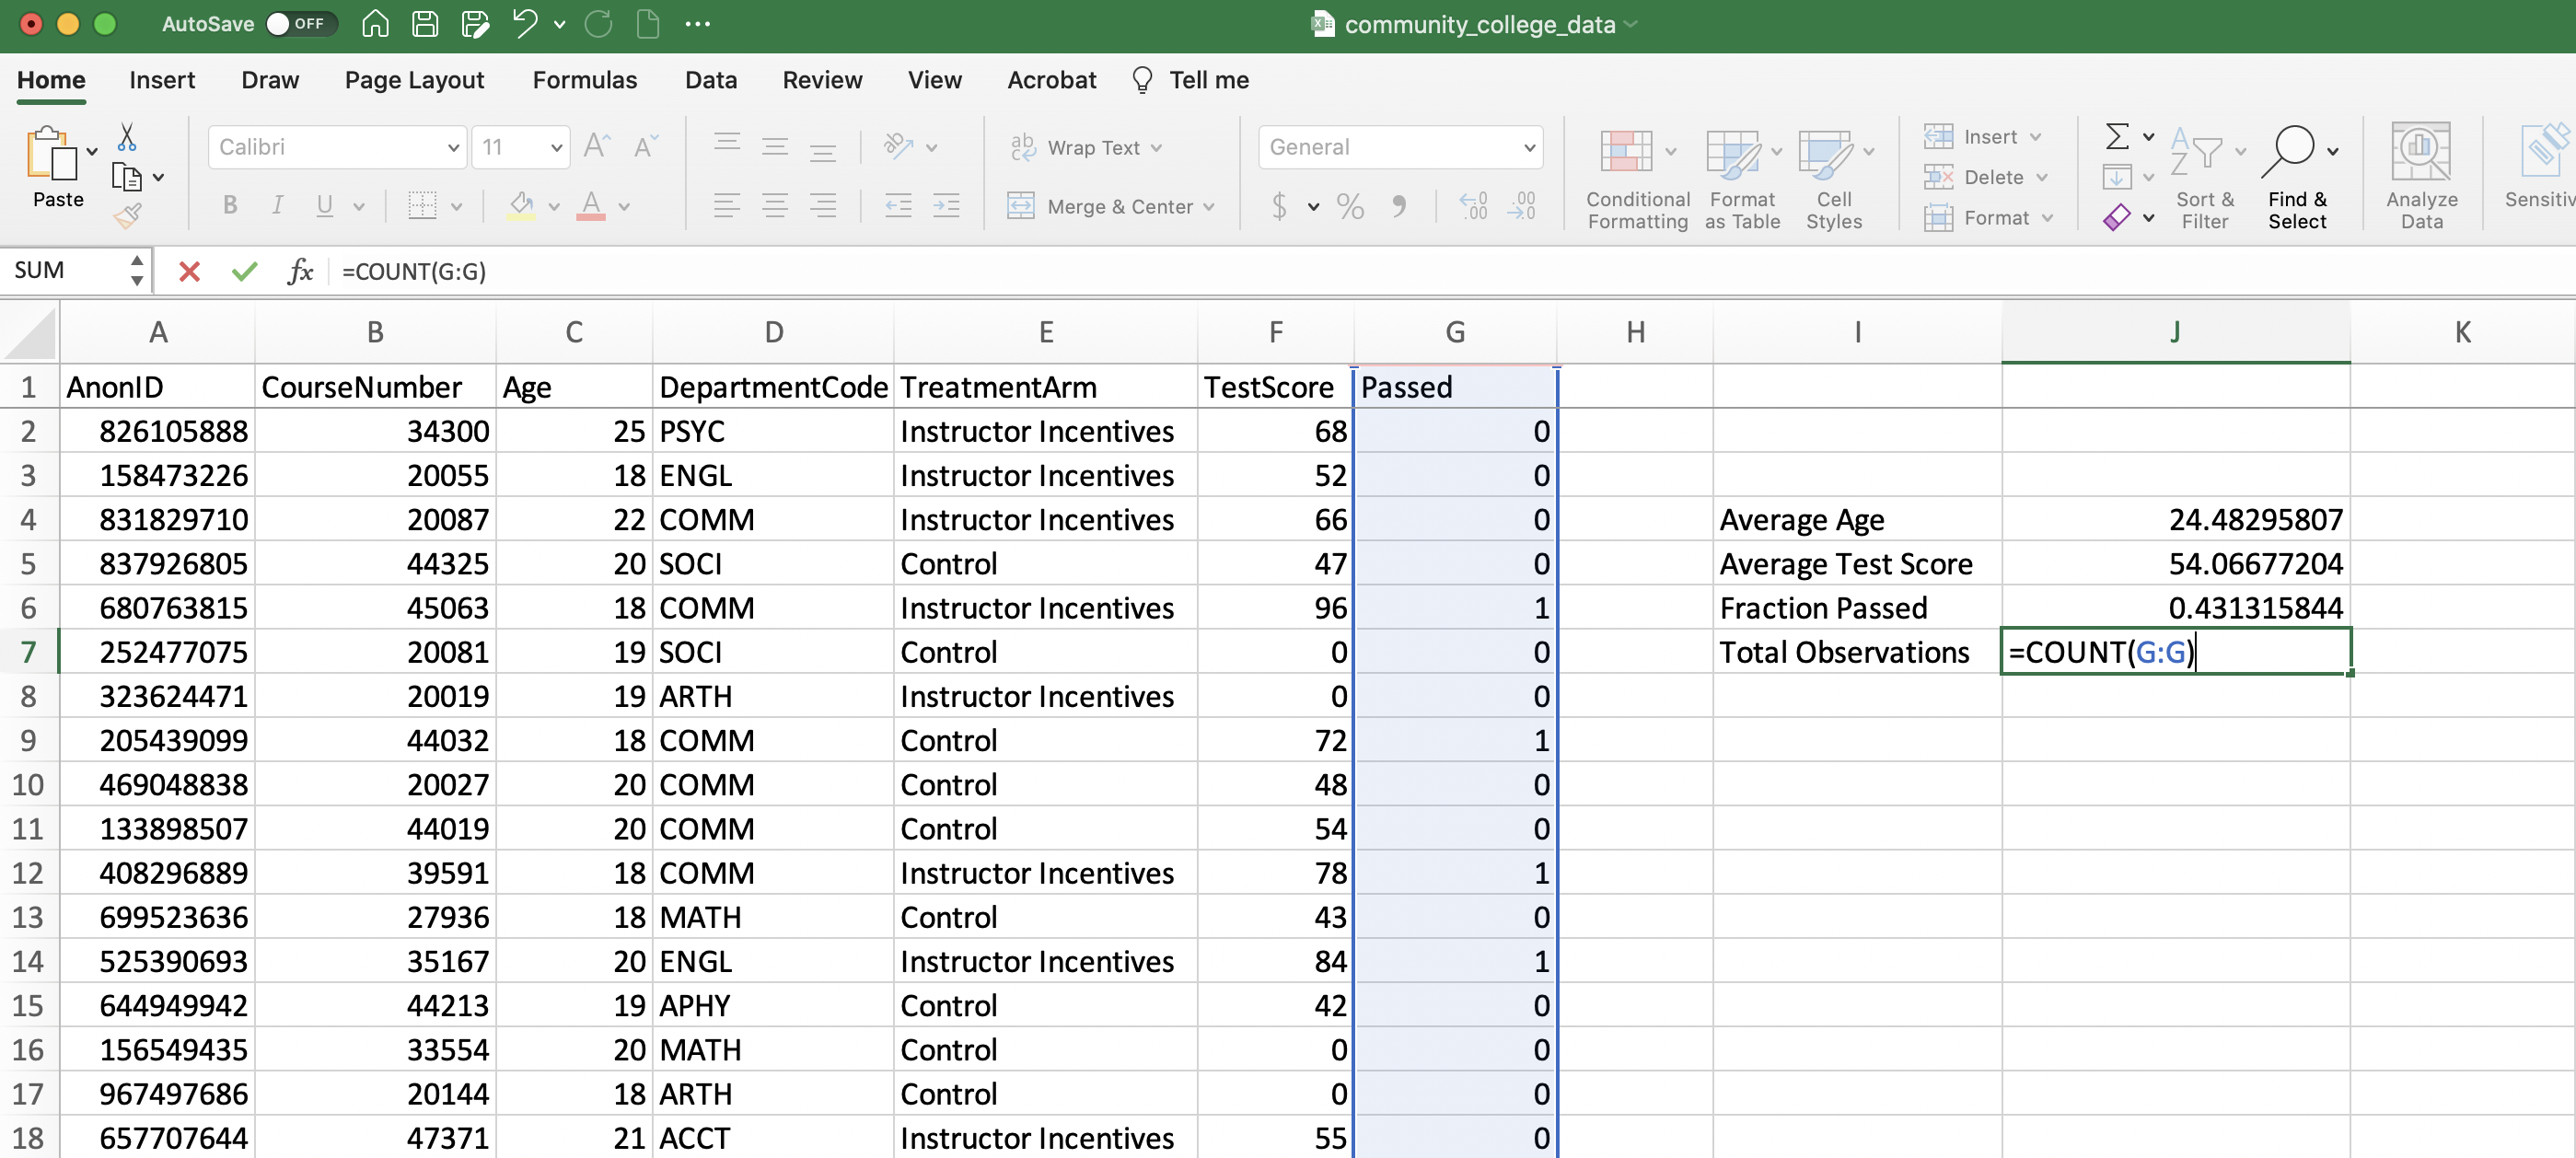
\includegraphics[width=1\linewidth]{images/01_count} 

}

\caption{Computing Total Observations}\label{fig:count}
\end{figure}

\section{Pivot Tables}\label{S:pivottables}

So far, we have learned to retrieve summary statistics using functions. This works very well for retrieving summary statistics for the entire dataset. Sometimes however we want more complicated summary statistics. For example, in our empirical application, we might be interested in passing rates for different departments. While it is possible to retrieve these using functions, an easier way is through a \textbf{pivot table}. The name ``pivot'' comes from ``pivoting'' the data into a format that provides useful information.

To understand what we are trying to accomplish with our pivot table, let's start by looking at our end goal in Figure \ref{fig:pivotfinal}. In the Pivot Table, each \textbf{row} is a separate department. Next to each department, we have the fraction of students who passed the standardized test in that department. The departments give different tests based on the material taught in the course, but a score of 70 or greater counts as a pass in all departments.

\begin{figure}

{\centering 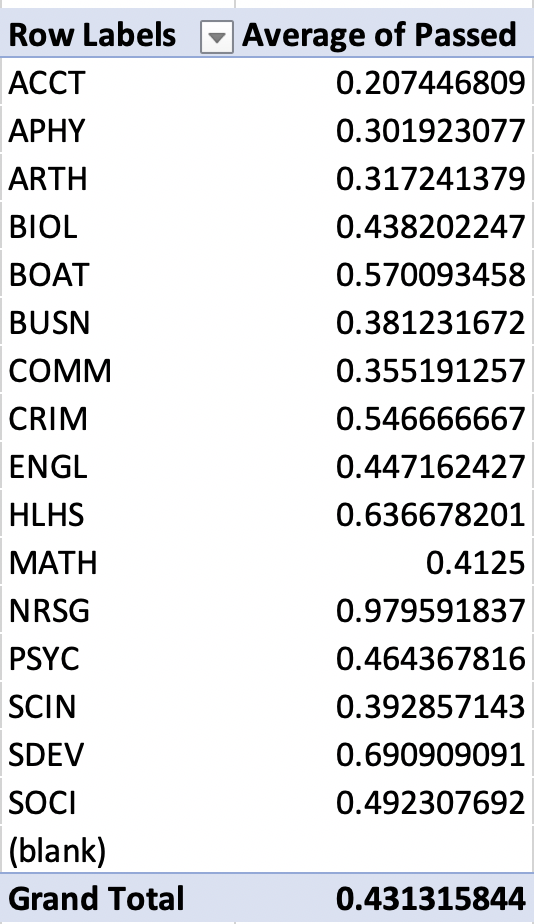
\includegraphics[width=0.38\linewidth]{images/01_pivot_final} 

}

\caption{Pivot Table: Pass Rates by Department}\label{fig:pivotfinal}
\end{figure}

Now let's go through how to construct Figure \ref{fig:pivotfinal}. To insert a pivot table, go to the Insert tab and click ``Insert Pivot Table'', as seen in Figure \ref{fig:pivot1}

\begin{figure}

{\centering 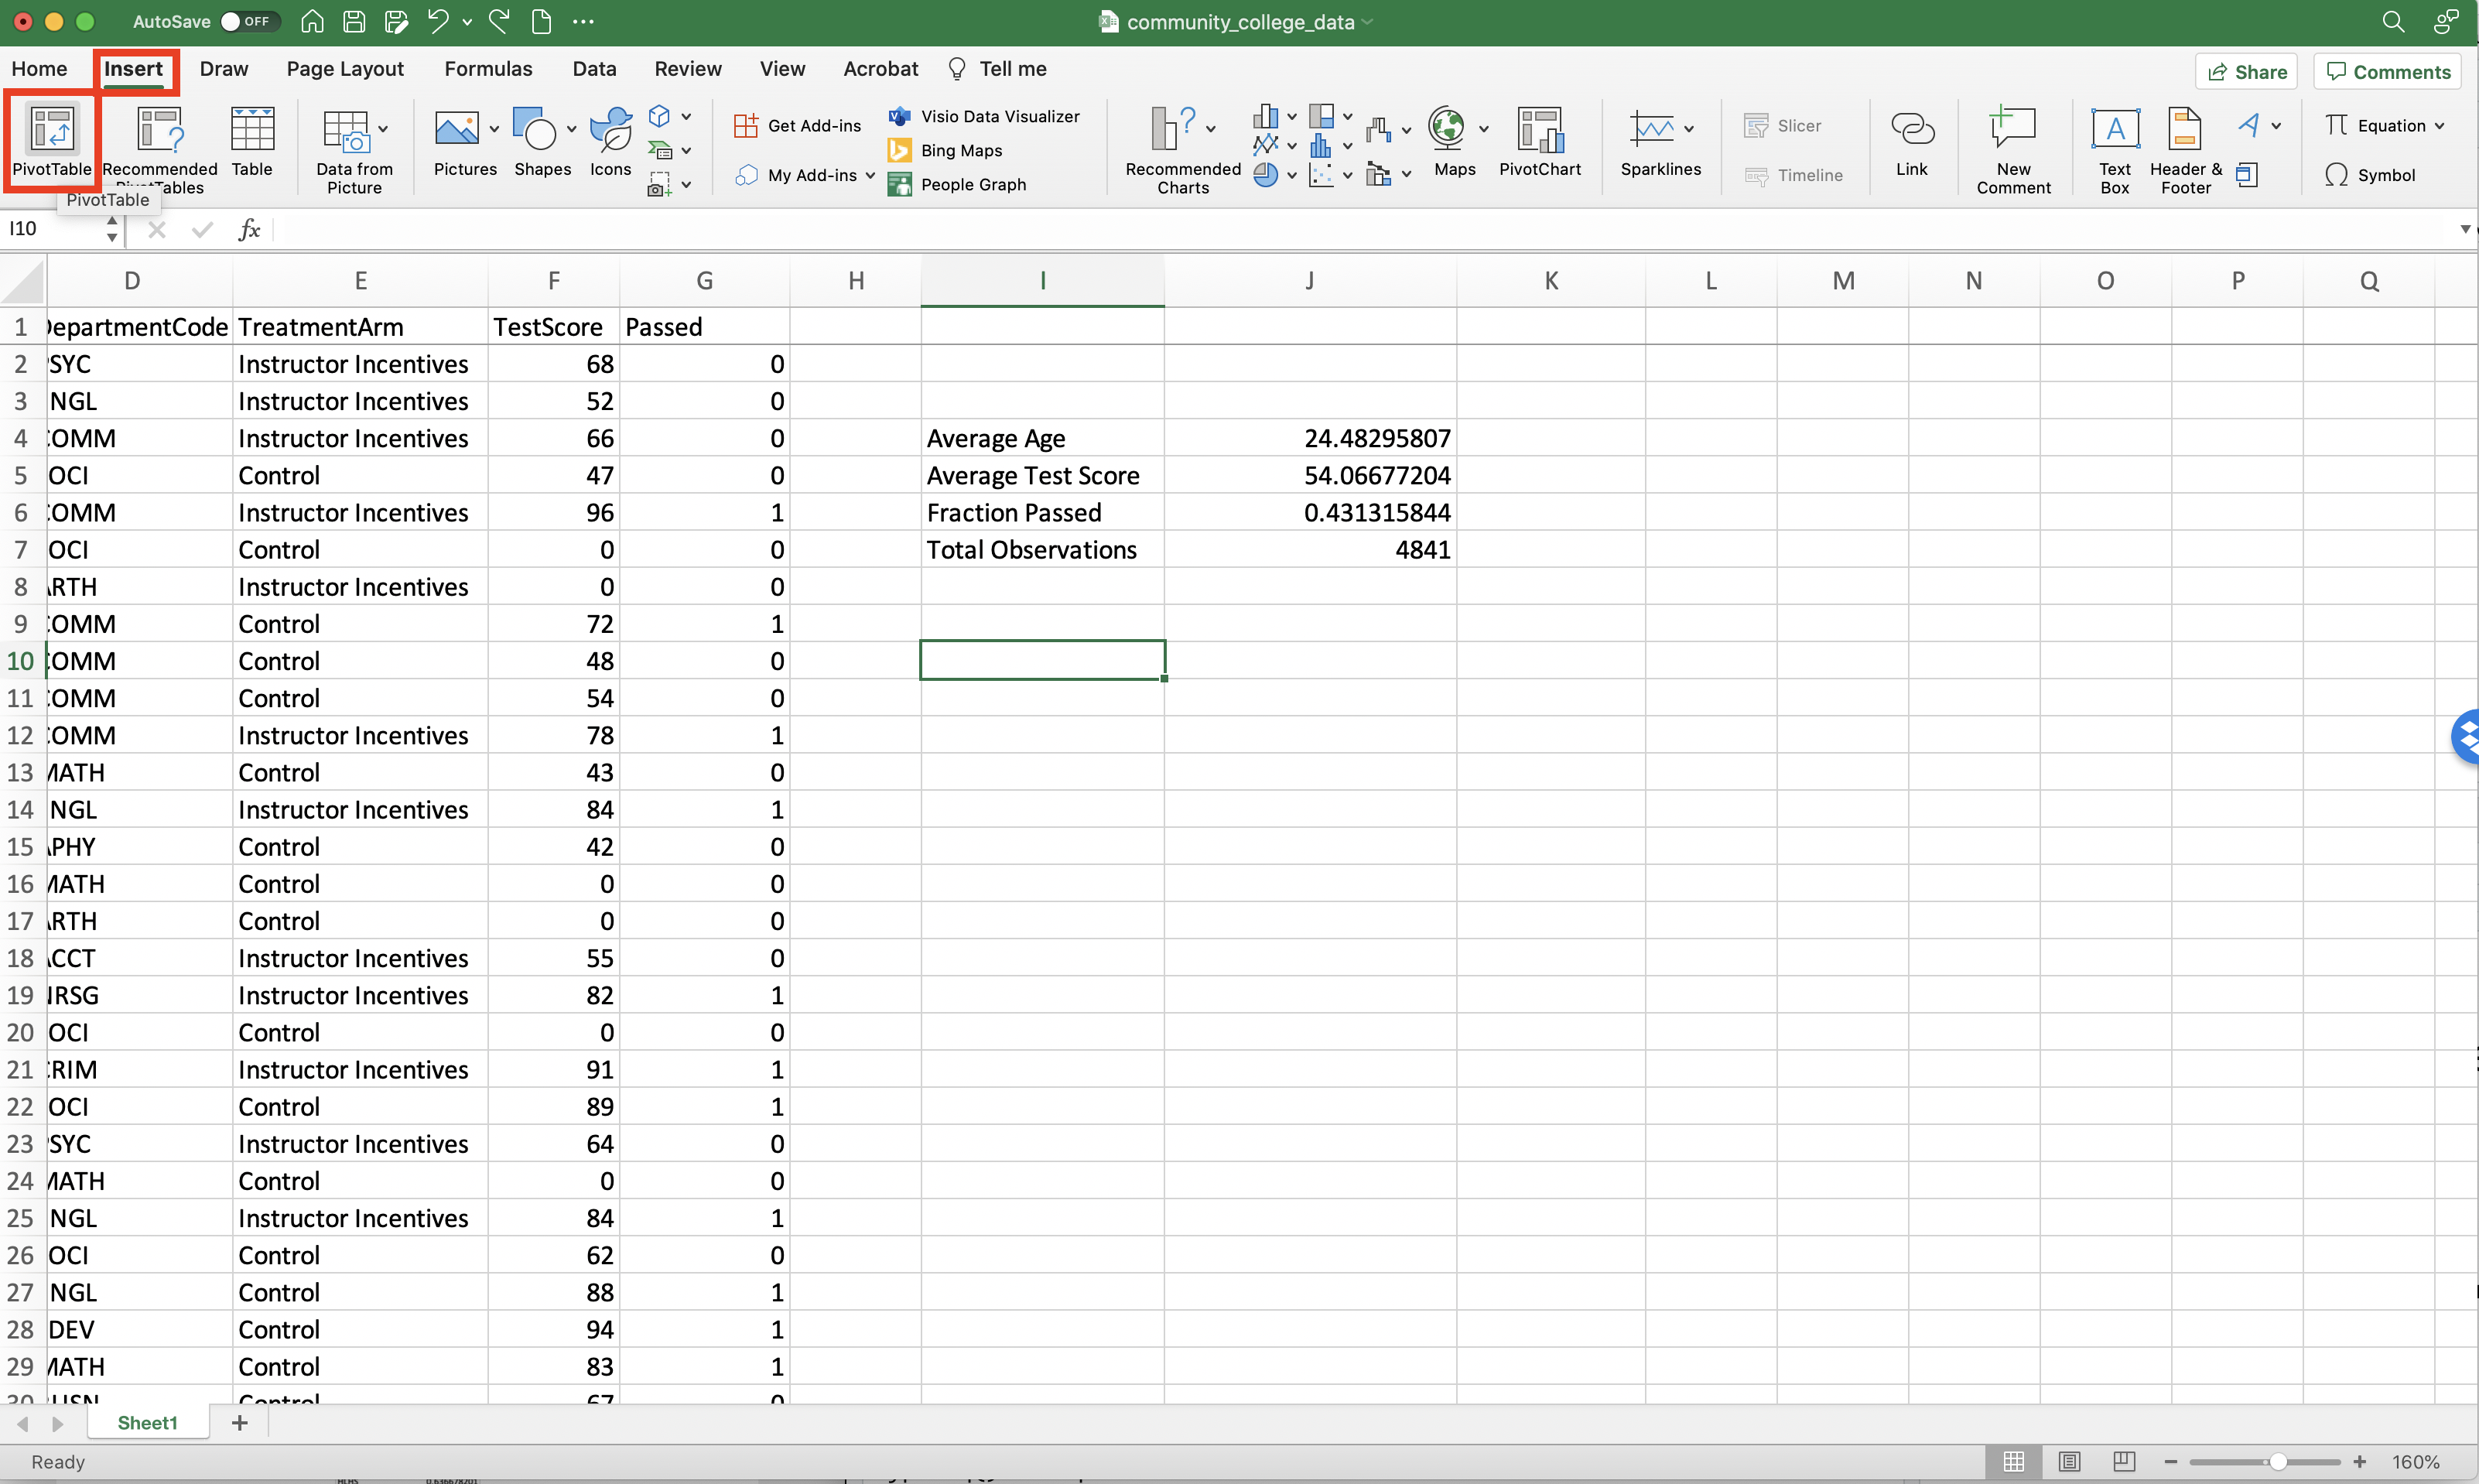
\includegraphics[width=1\linewidth]{images/01_pivot1} 

}

\caption{Inserting a Pivot Table}\label{fig:pivot1}
\end{figure}

Next, you need to select a table or range. You should select all of the variables that you want to be in your pivot table. In our case, we need to have both the department and whether an individual passed. To select a range, we can click on a column (for example D), hold down, and then drag to another column (for example G). Since we began at D and dragged to G, the variables \texttt{DepartmentCode}, \texttt{TreatmentArm}, \texttt{TestScore}, and \texttt{Passed} will all be variables that we can include in the pivot table.

\begin{figure}

{\centering 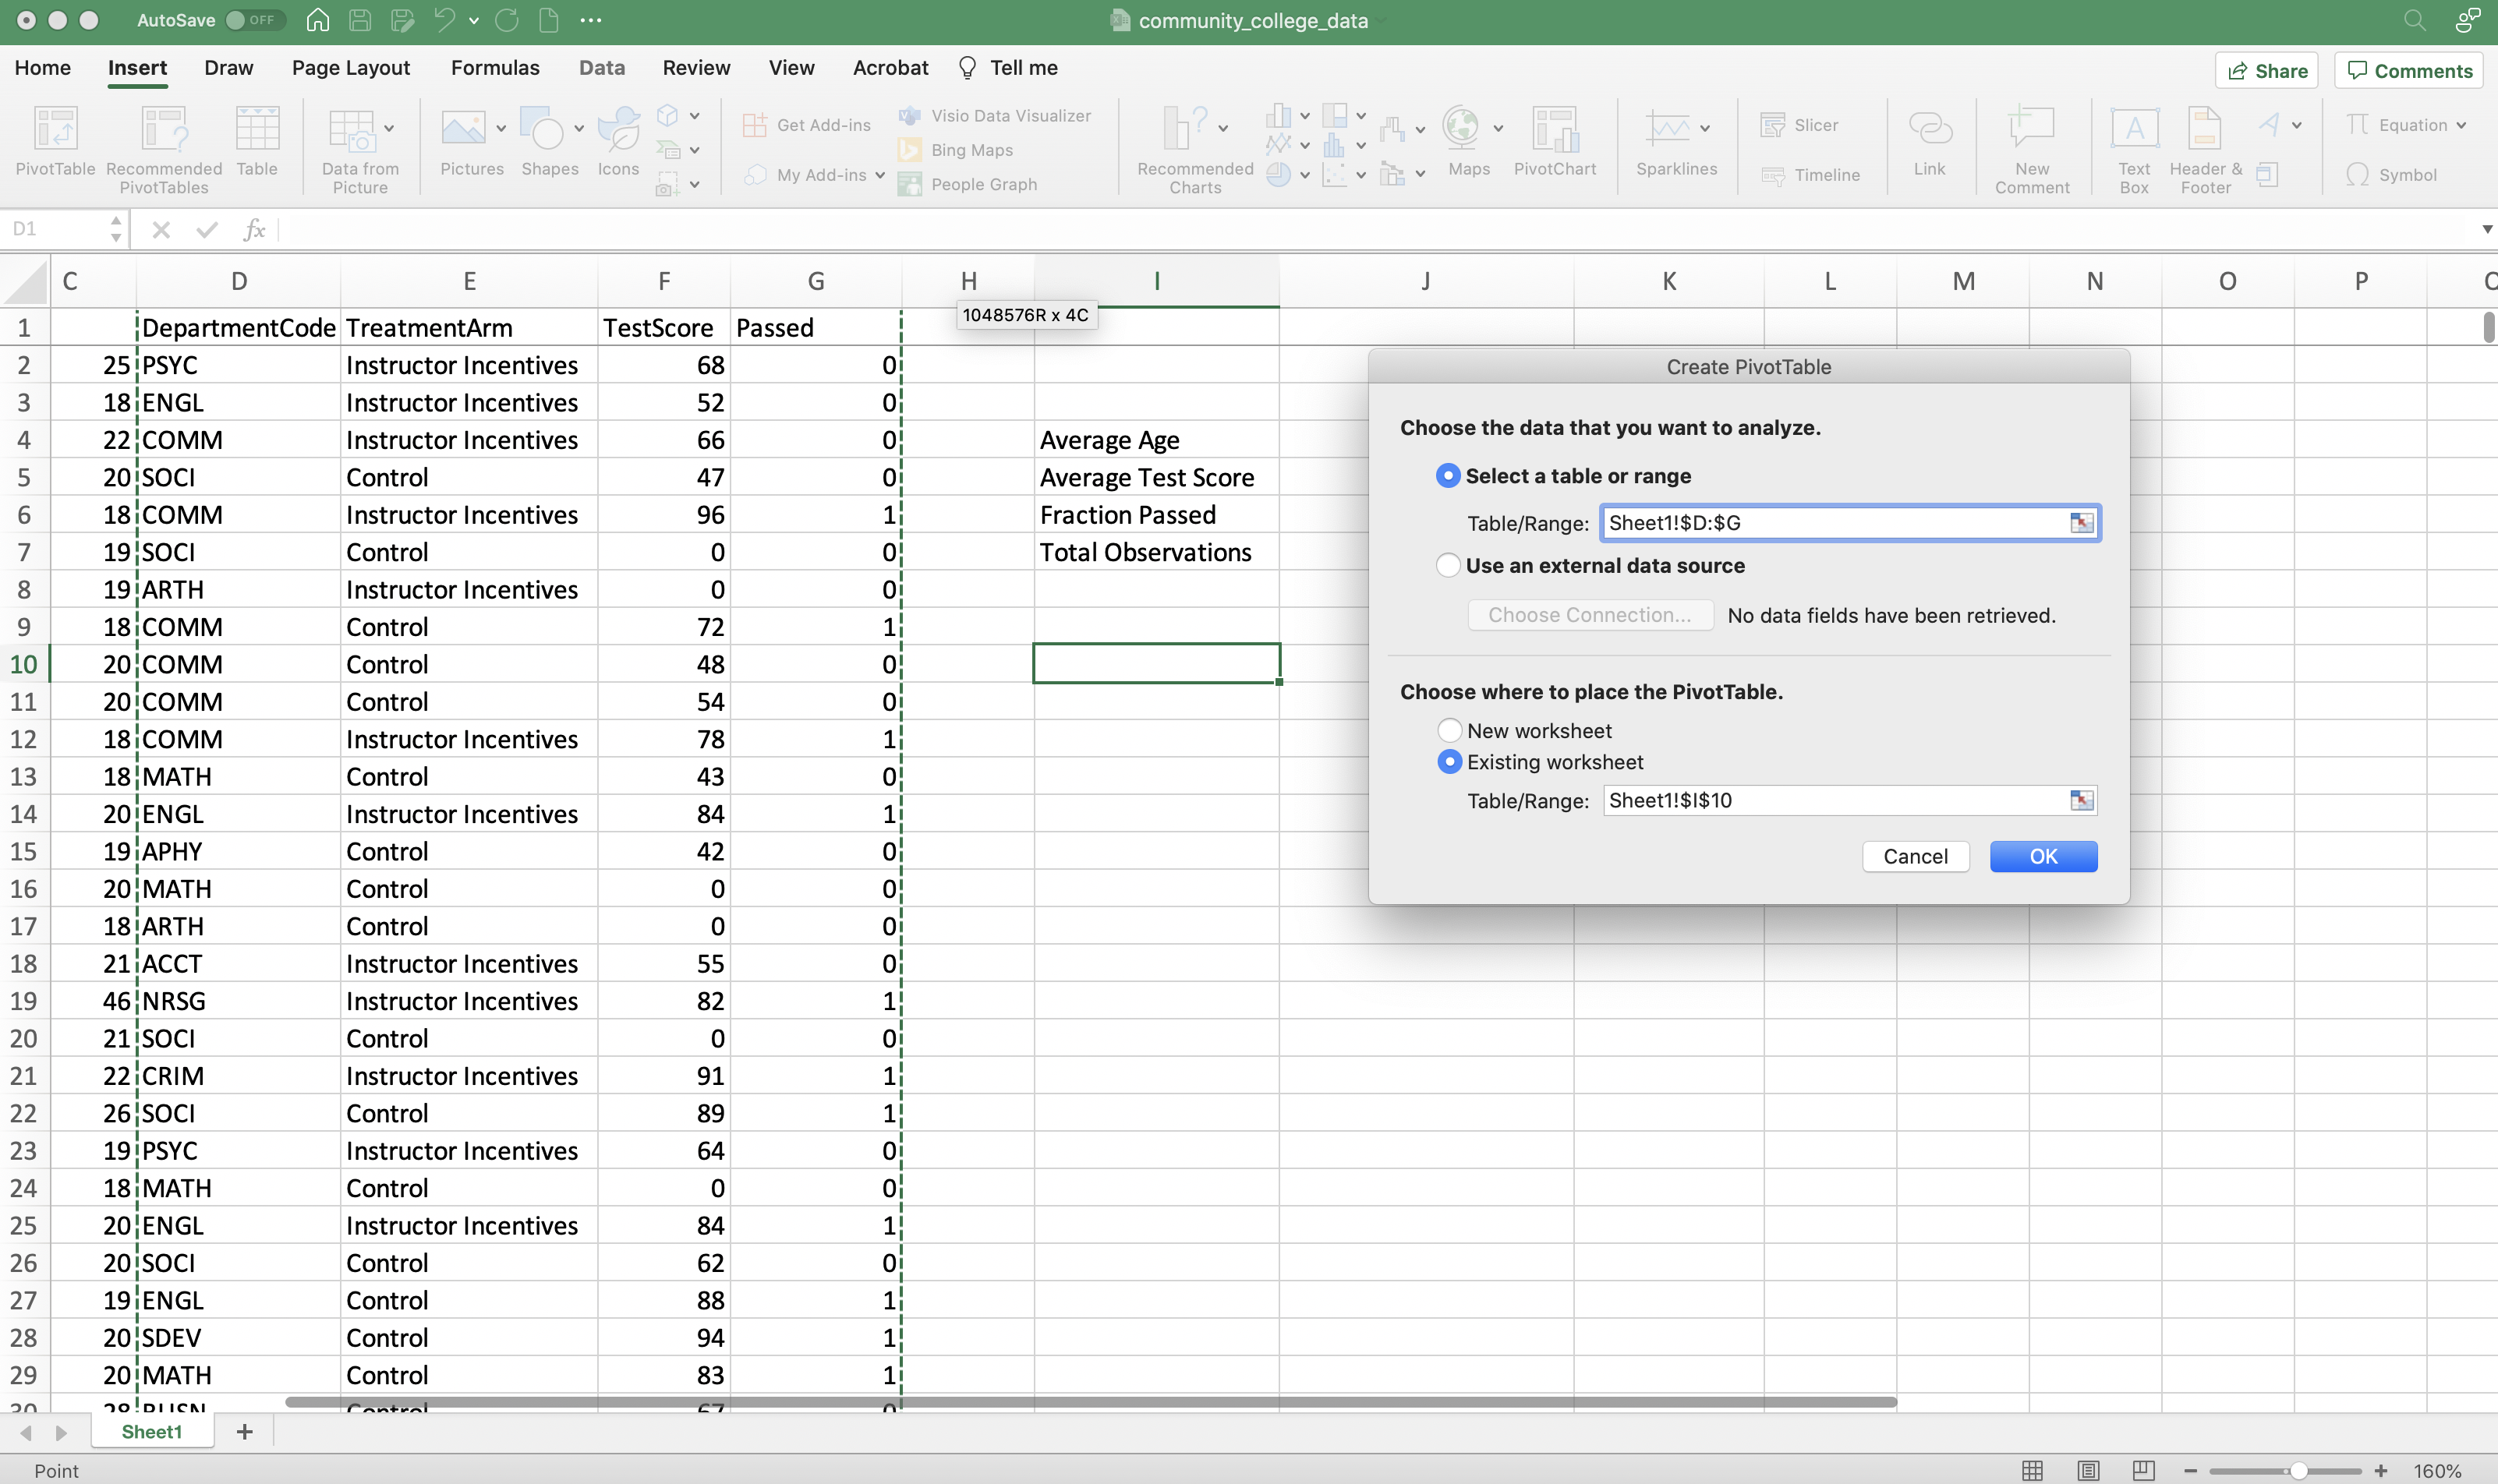
\includegraphics[width=1\linewidth]{images/01_pivot3} 

}

\caption{Selecting a Range for the Pivot Table}\label{fig:pivot3}
\end{figure}

You can also choose where you would like your pivot table to appear. By default, the table will be placed in whichever cell you clicked last (in my case this is cell \texttt{I10}). Therefore, before you insert a pivot table, you should click the cell where you would like it to appear.

As can be seen in Figure \ref{fig:pivot4}, Excel has drawn a blank Pivot table. On the right, we can see the new panel ``PivotTable Fields'' which we will use to build our Pivot table.

\begin{figure}

{\centering 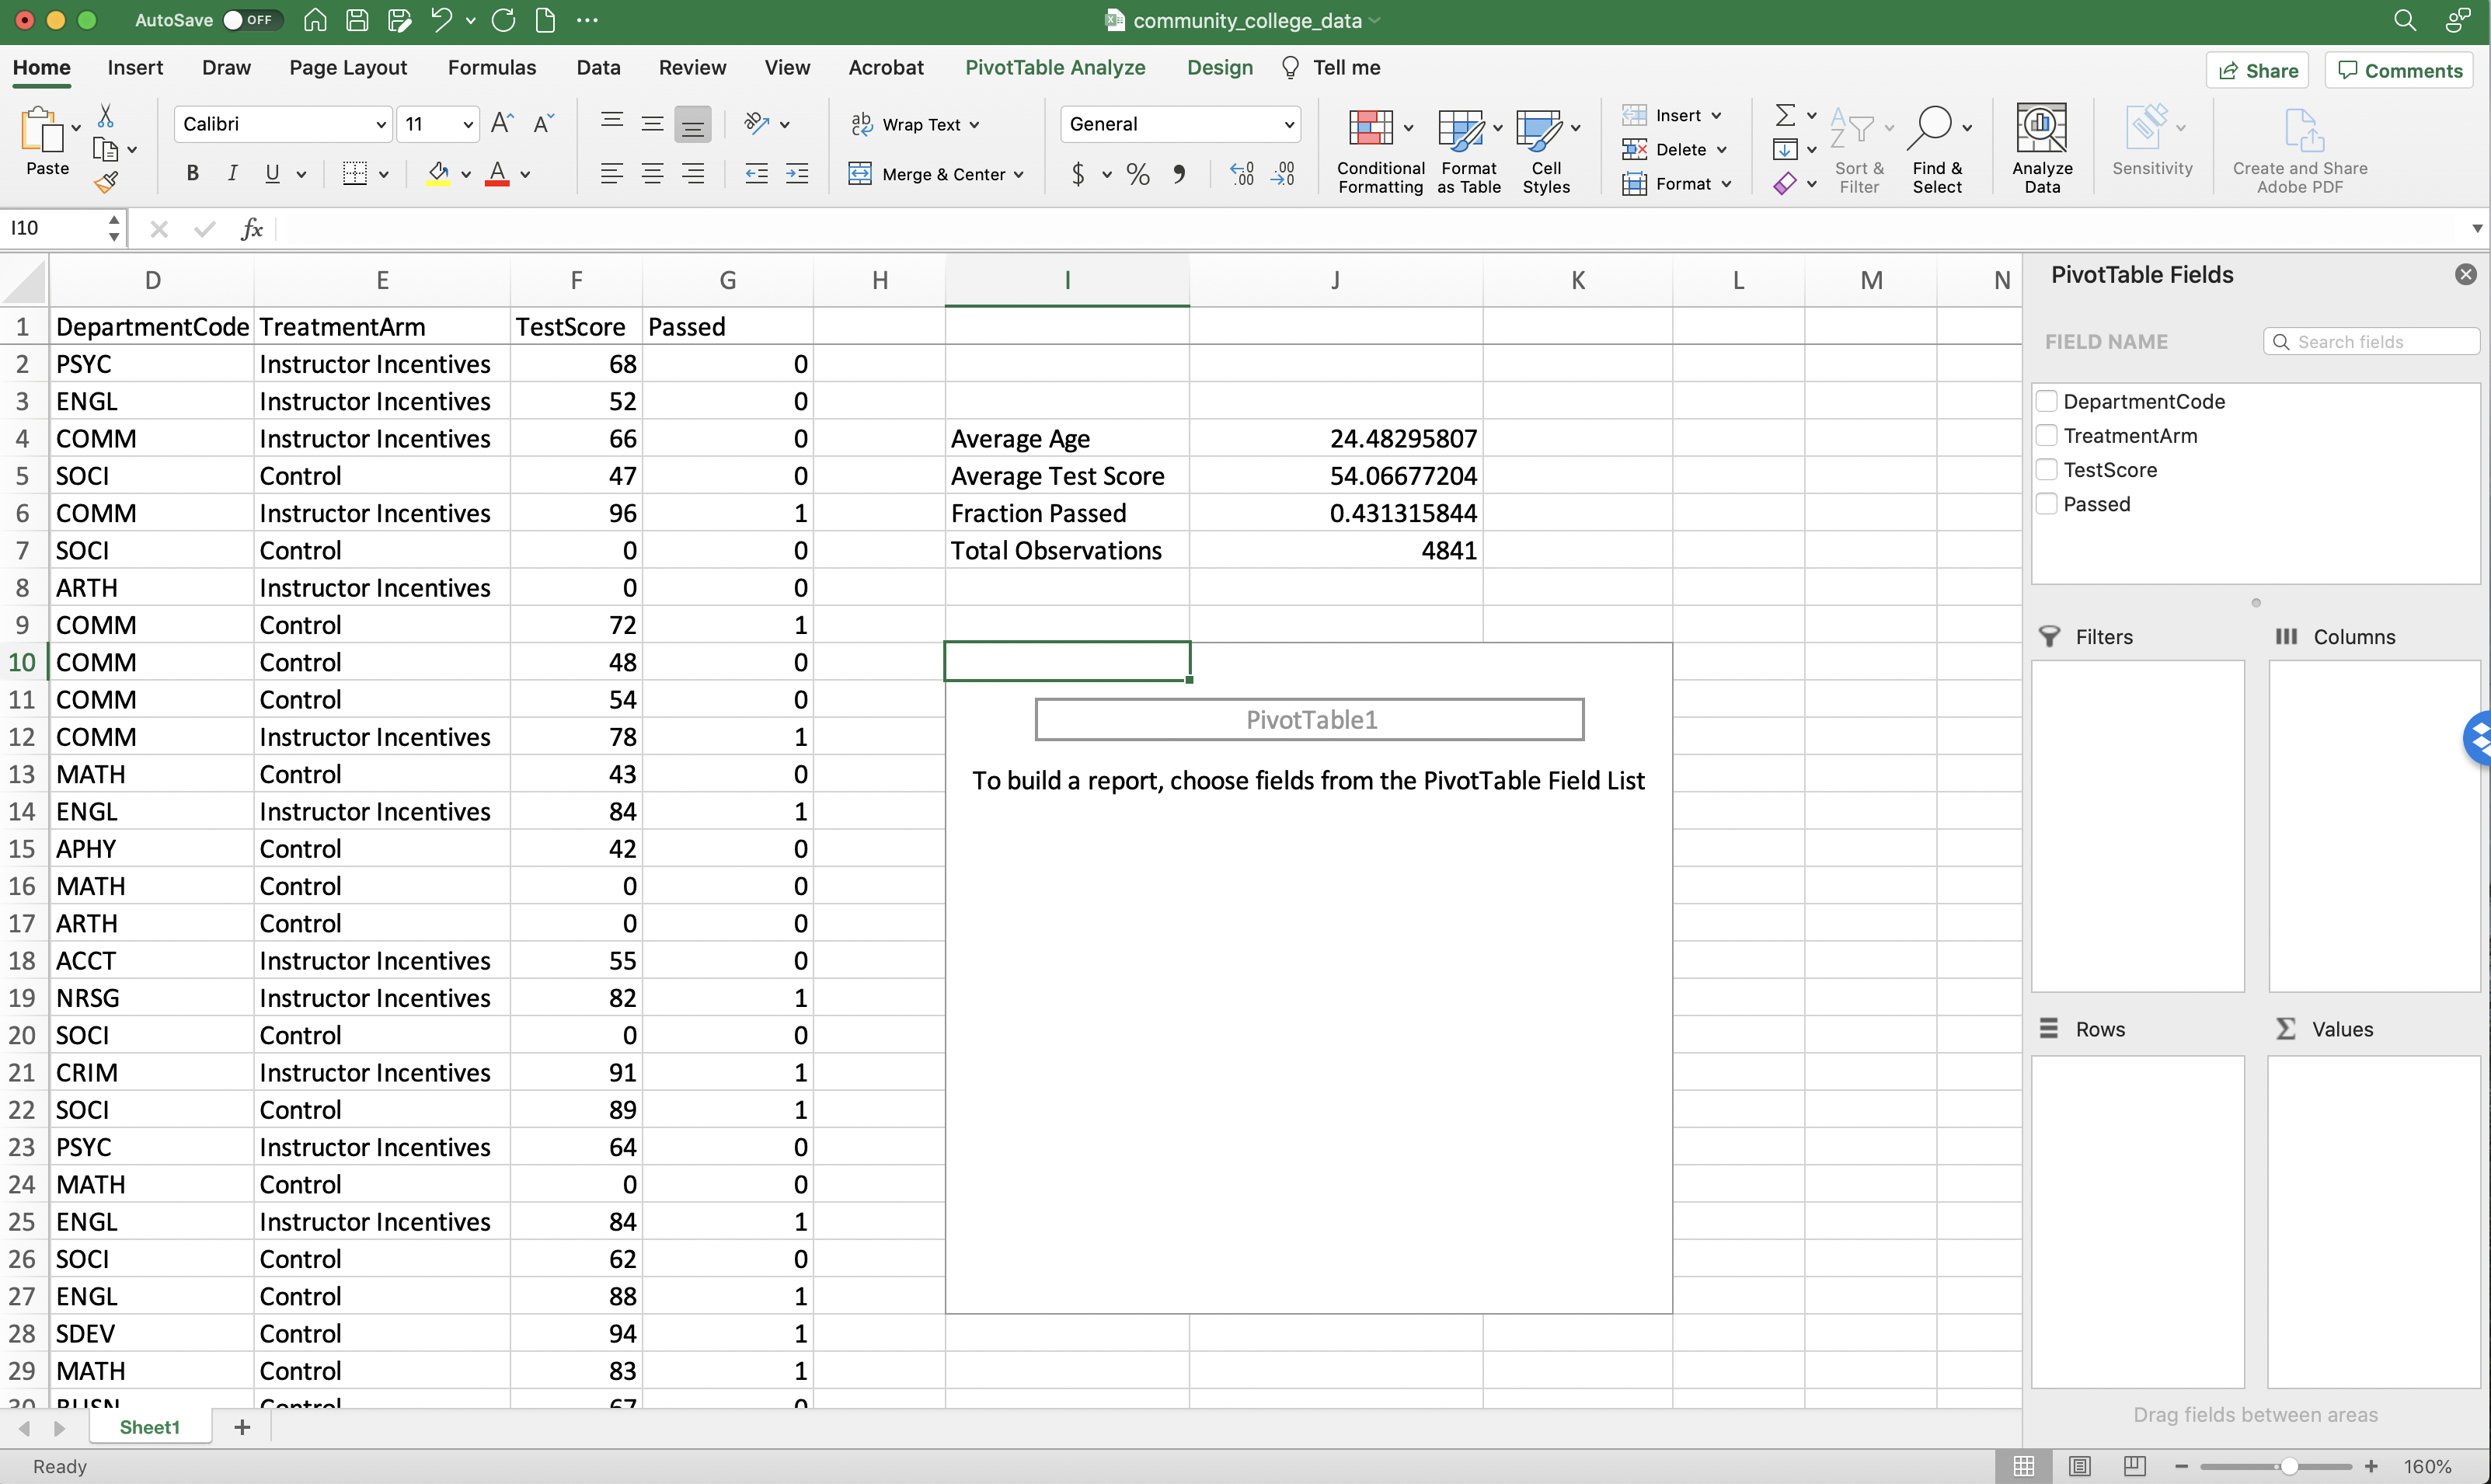
\includegraphics[width=1\linewidth]{images/01_pivot4} 

}

\caption{A Blank Pivot Table}\label{fig:pivot4}
\end{figure}

We want each row in our pivot table to be a Department Code. So click the box next to \texttt{DepartmentCode} to put it into the pivot table.

\begin{figure}

{\centering 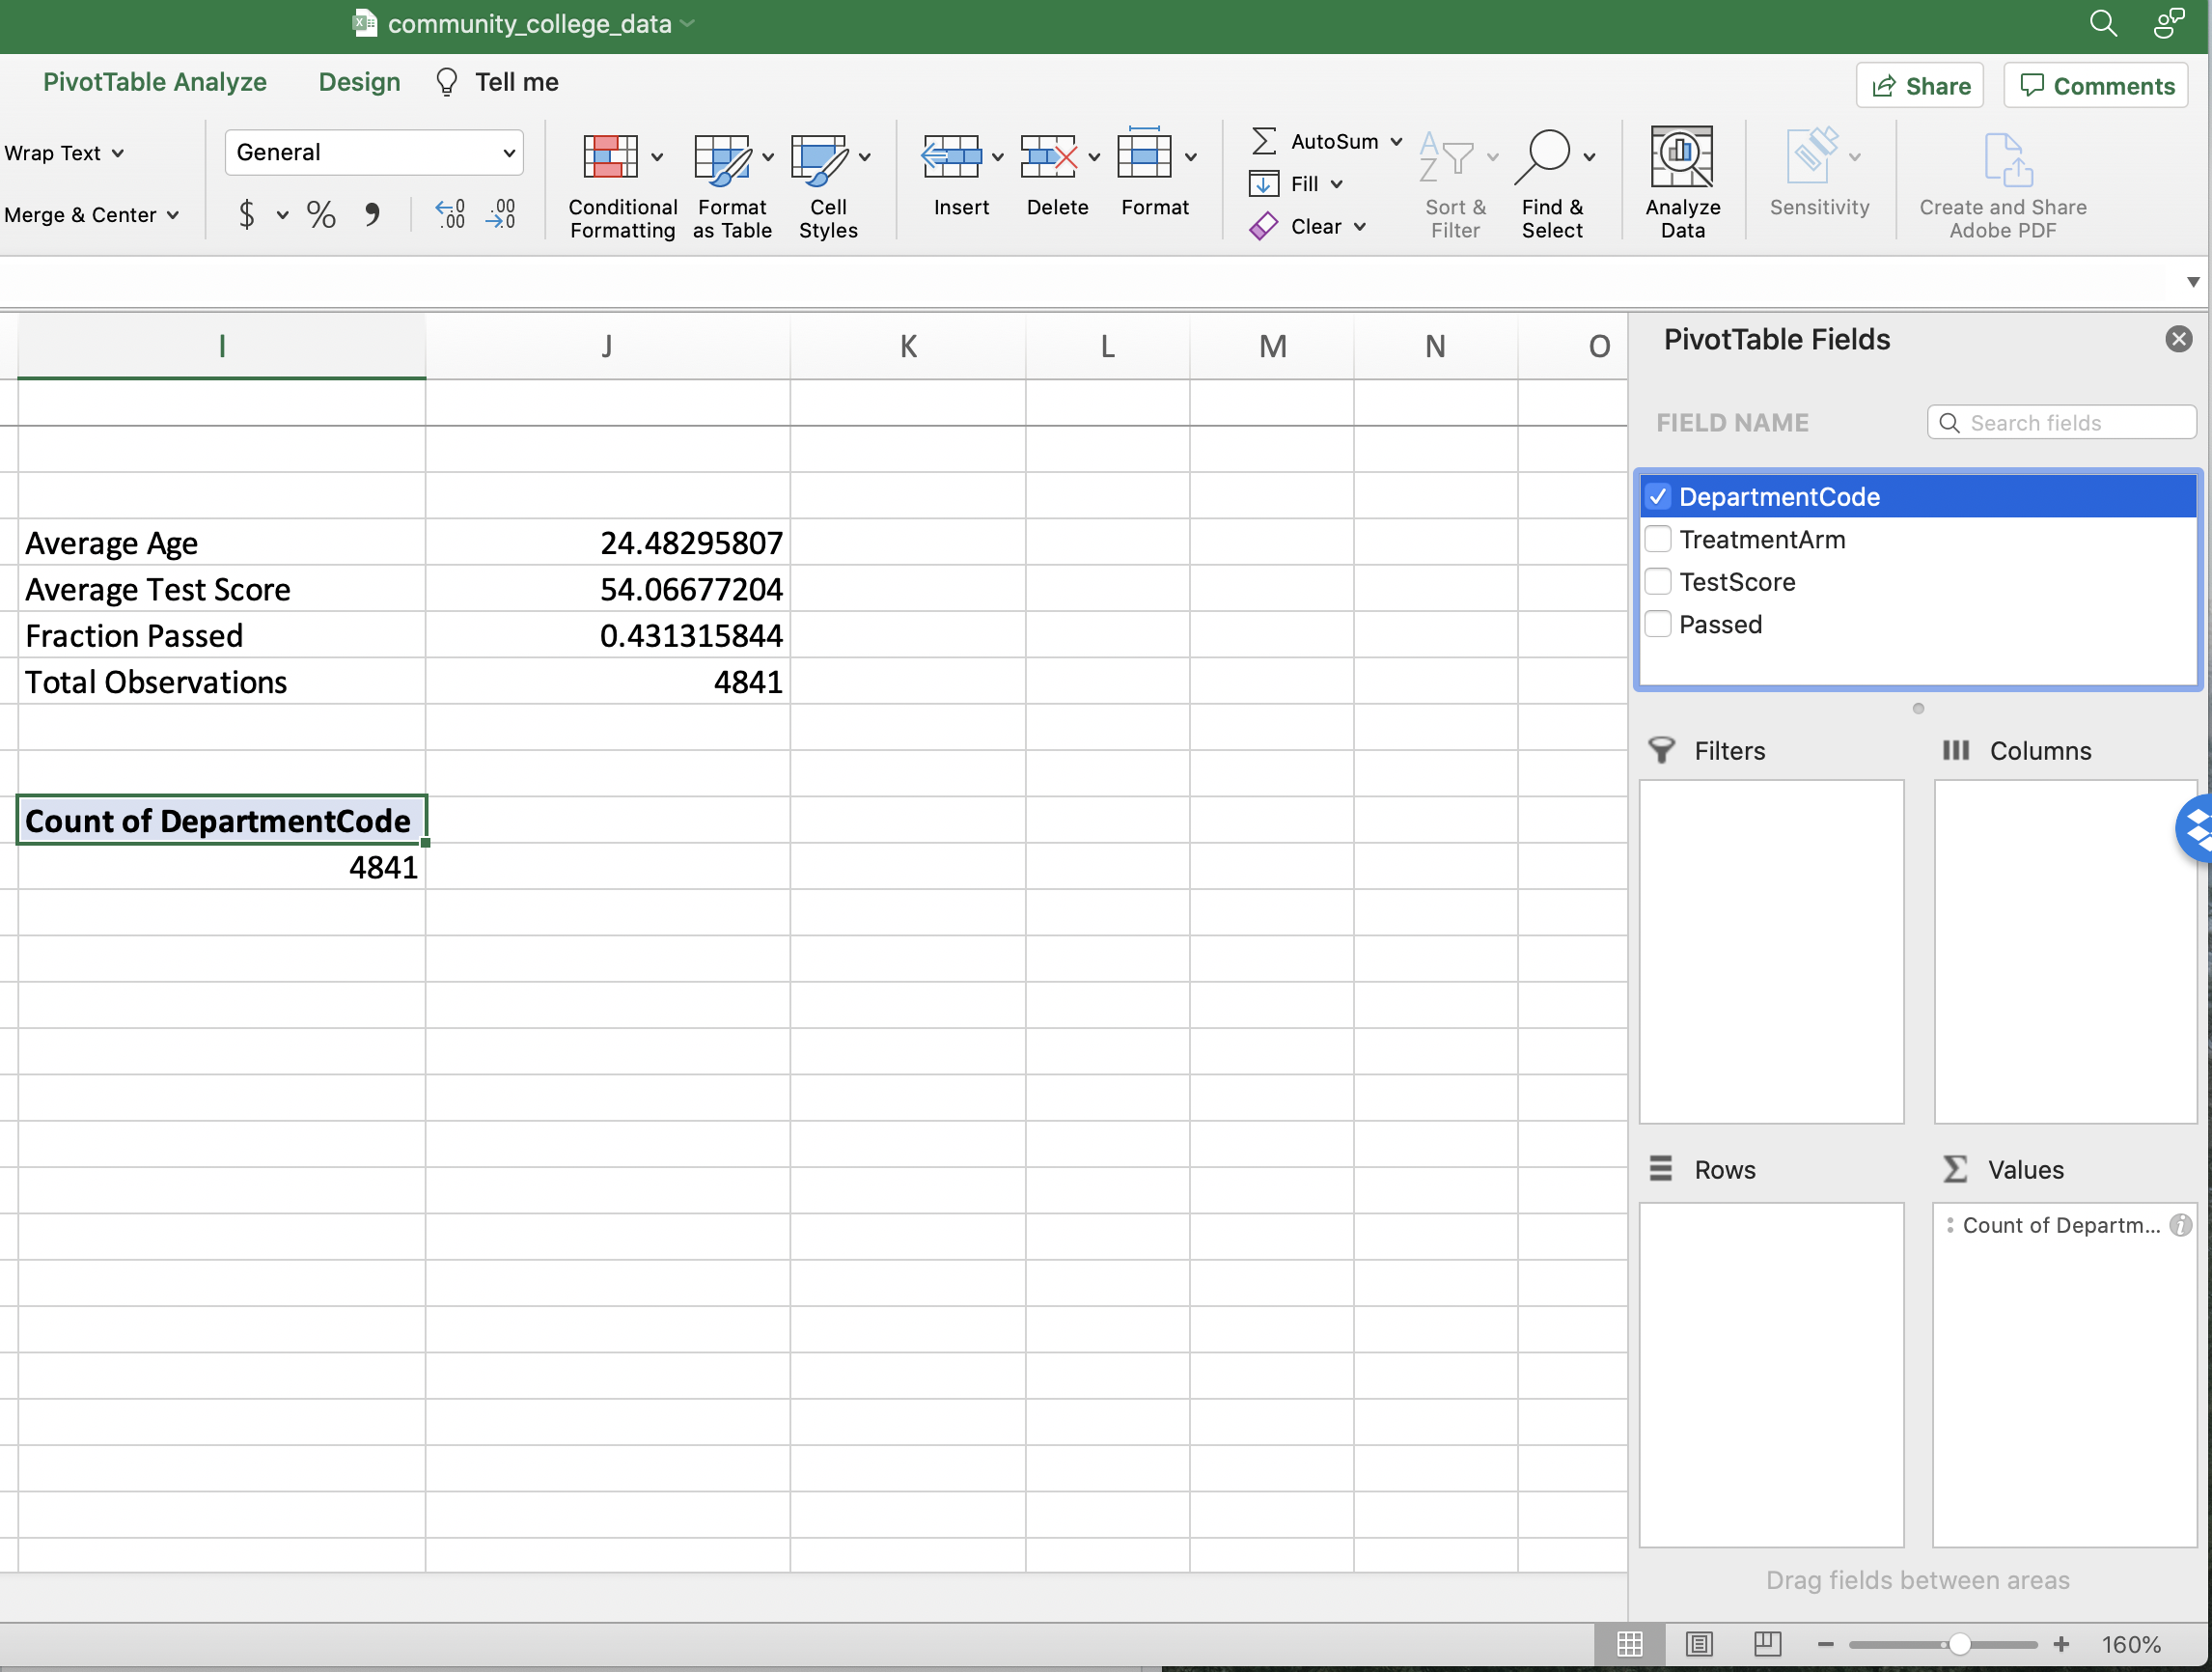
\includegraphics[width=1\linewidth]{images/01_pivot5} 

}

\caption{Adding DepartmentCode to the Pivot Table}\label{fig:pivot5}
\end{figure}

By default (see Figure \ref{fig:pivot5}), Excel has placed this variable into the Values panel, but we want it to be in the Rows panel. We can move variables between these windows by clicking and dragging. In this example, we want to move \texttt{DepartmentCode} to the Rows panel.

\begin{figure}

{\centering 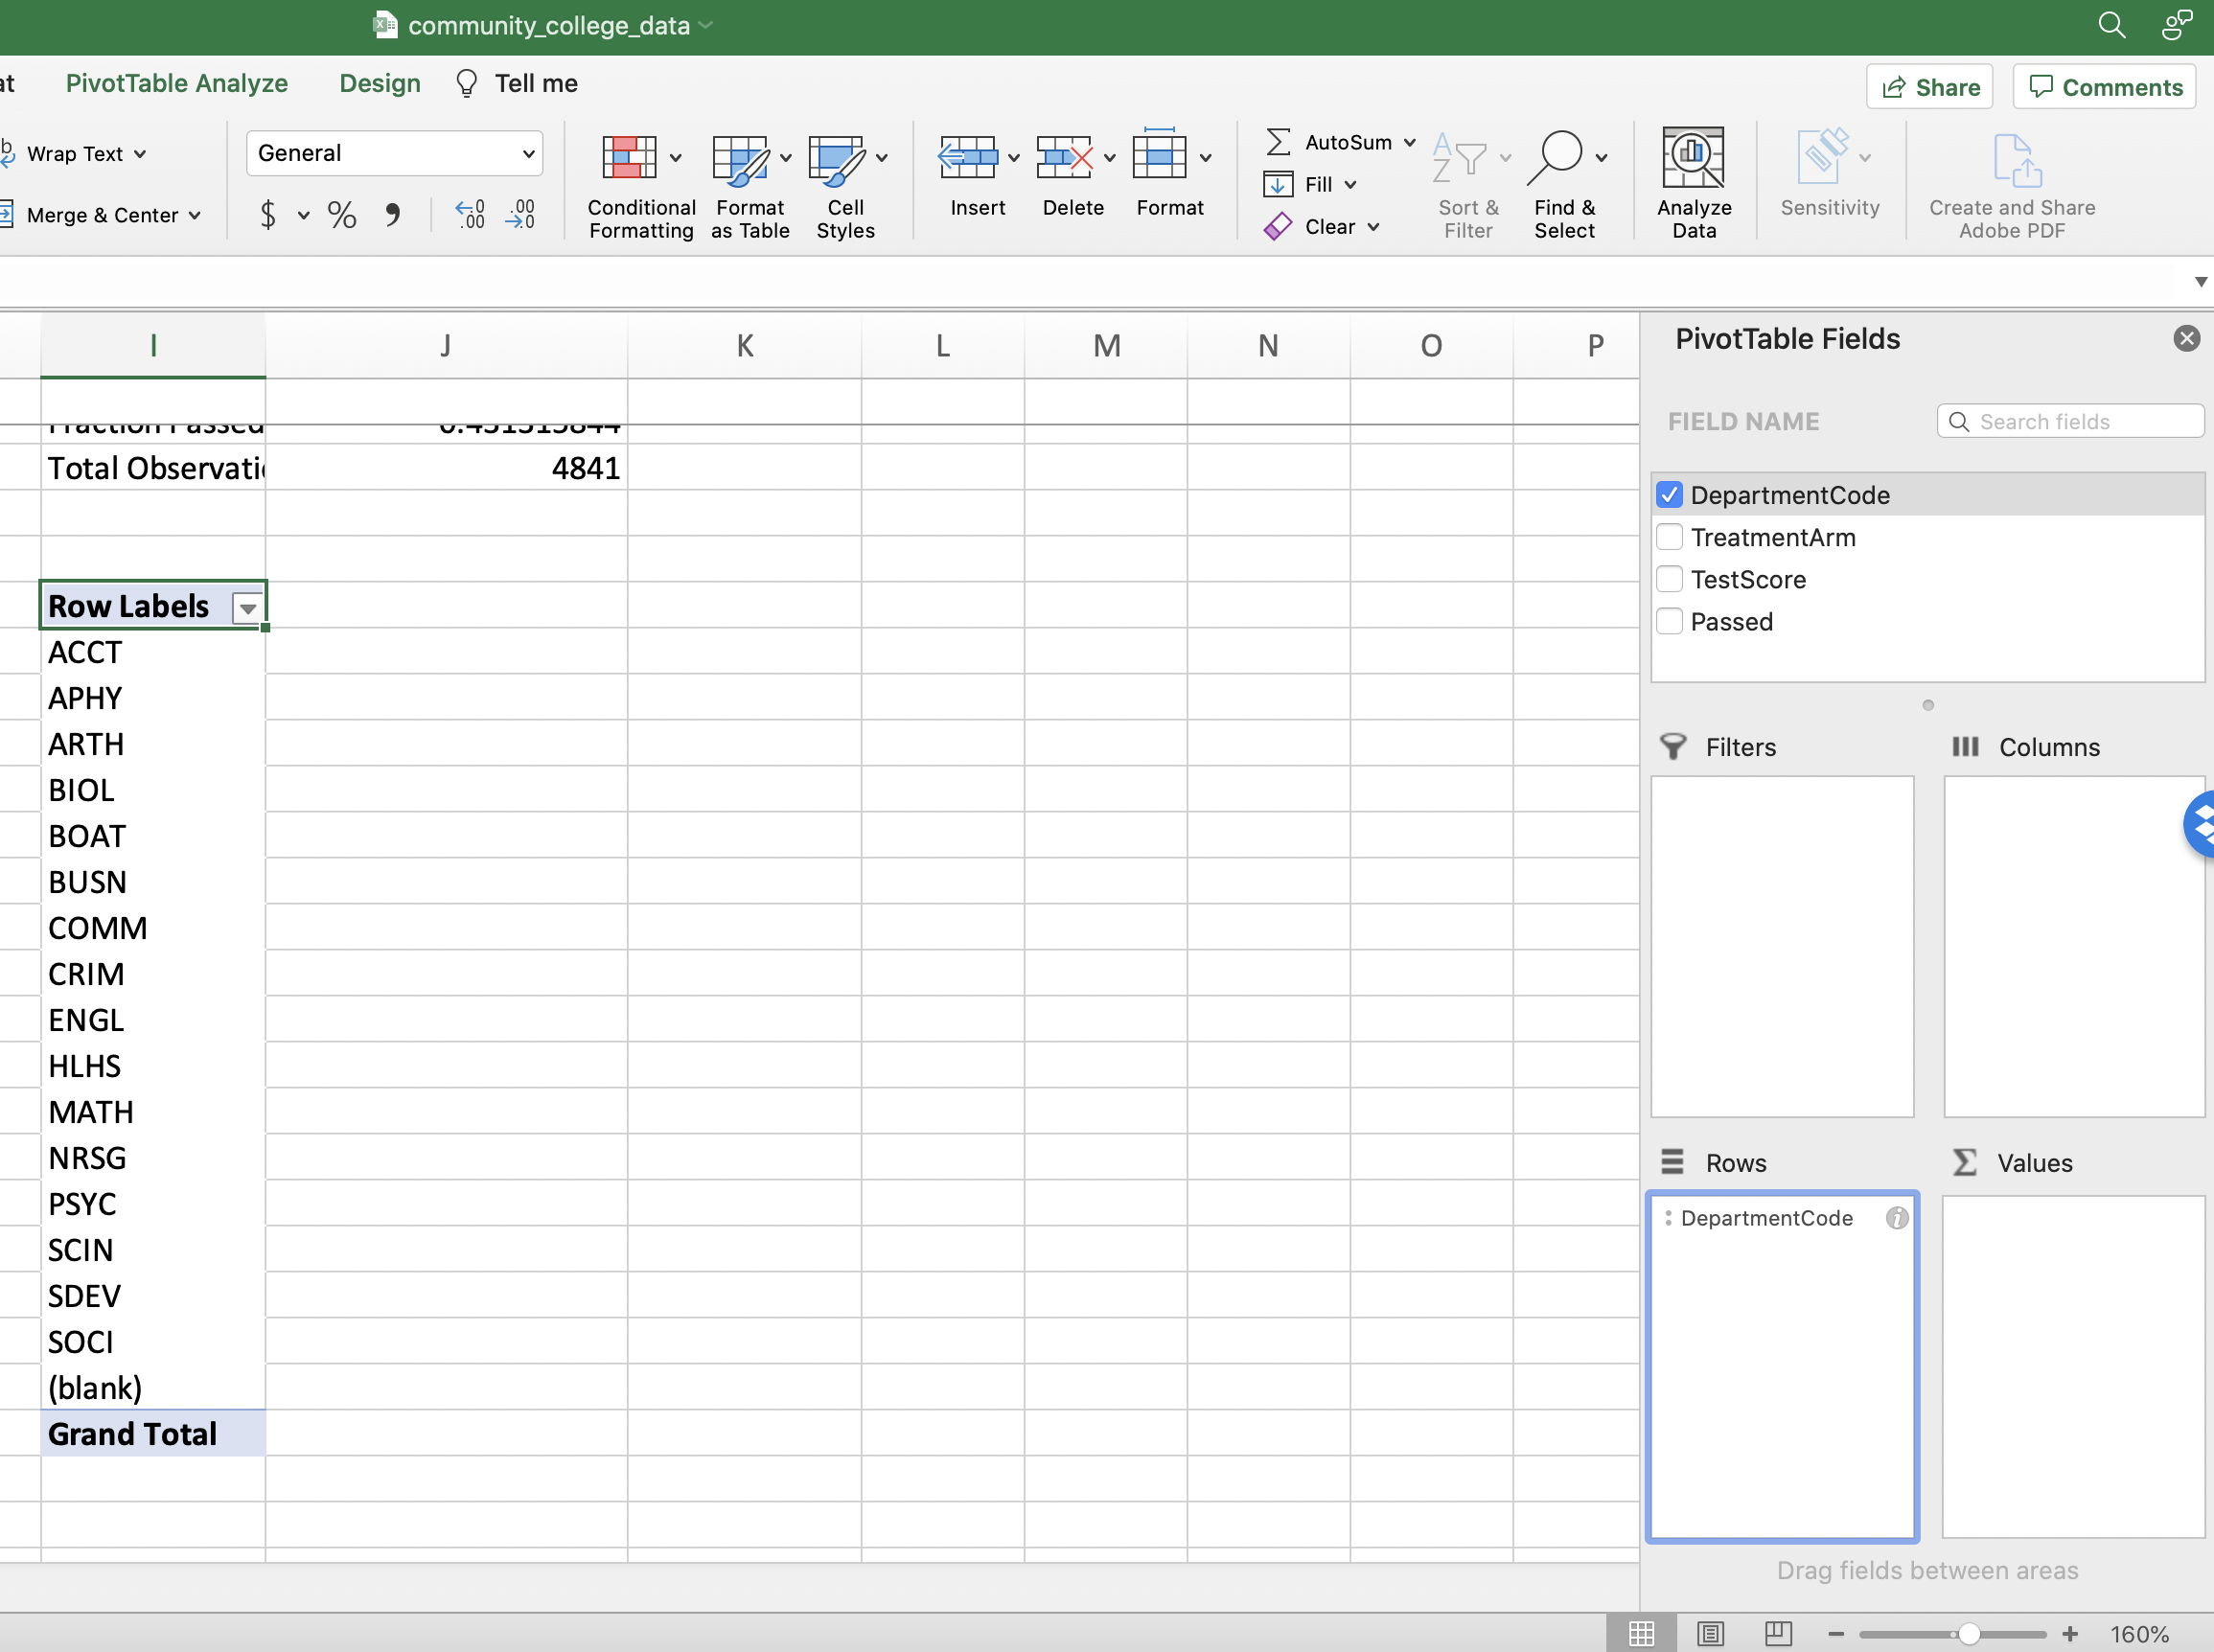
\includegraphics[width=1\linewidth]{images/01_pivot6} 

}

\caption{Adding DepartmentCode to the Pivot Table}\label{fig:pivot6}
\end{figure}

In the Values panel, we want pass rates. We will compute these pass rates from the variable ``Passed''

\begin{figure}

{\centering 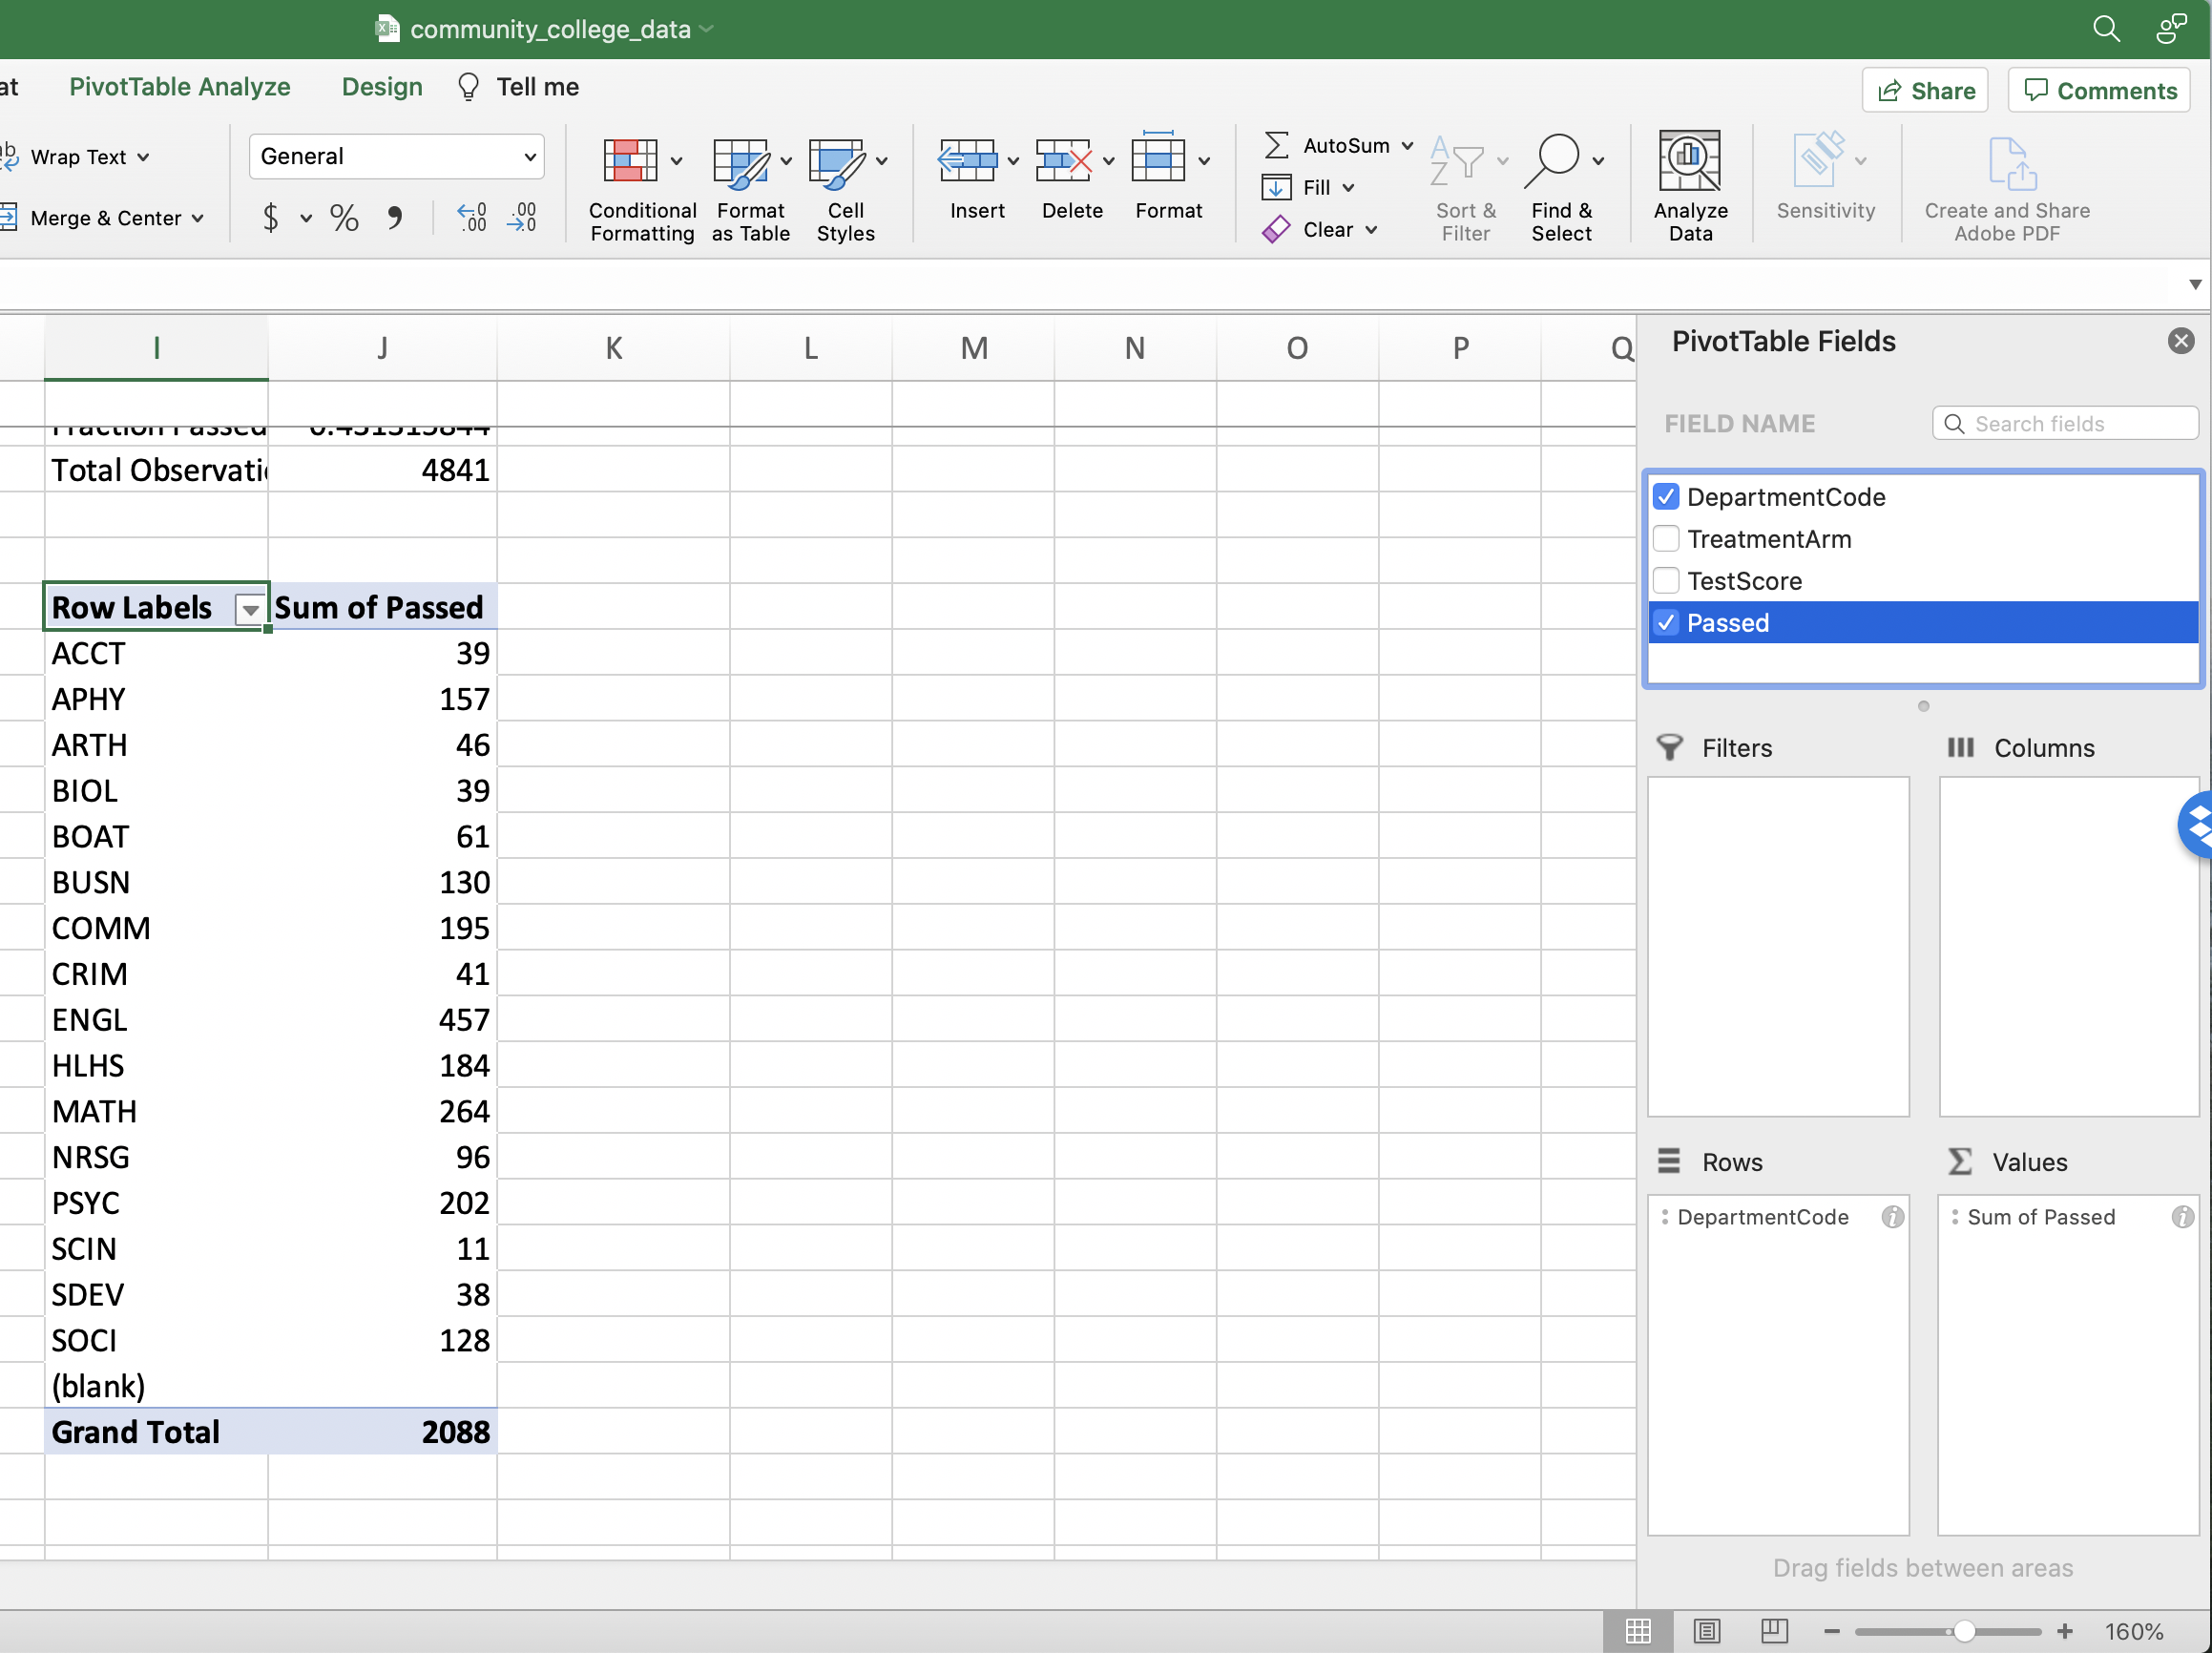
\includegraphics[width=1\linewidth]{images/01_pivot7} 

}

\caption{Adding Passed to the Pivot Table}\label{fig:pivot7}
\end{figure}

By default Excel is displaying the ``SUM'' by department (i.e.~number of individuals that passed, not the fraction that passed). To change the displayed statistic click the ``i'' next to the ``Values'' label and then select ``Average''.

\begin{figure}

{\centering 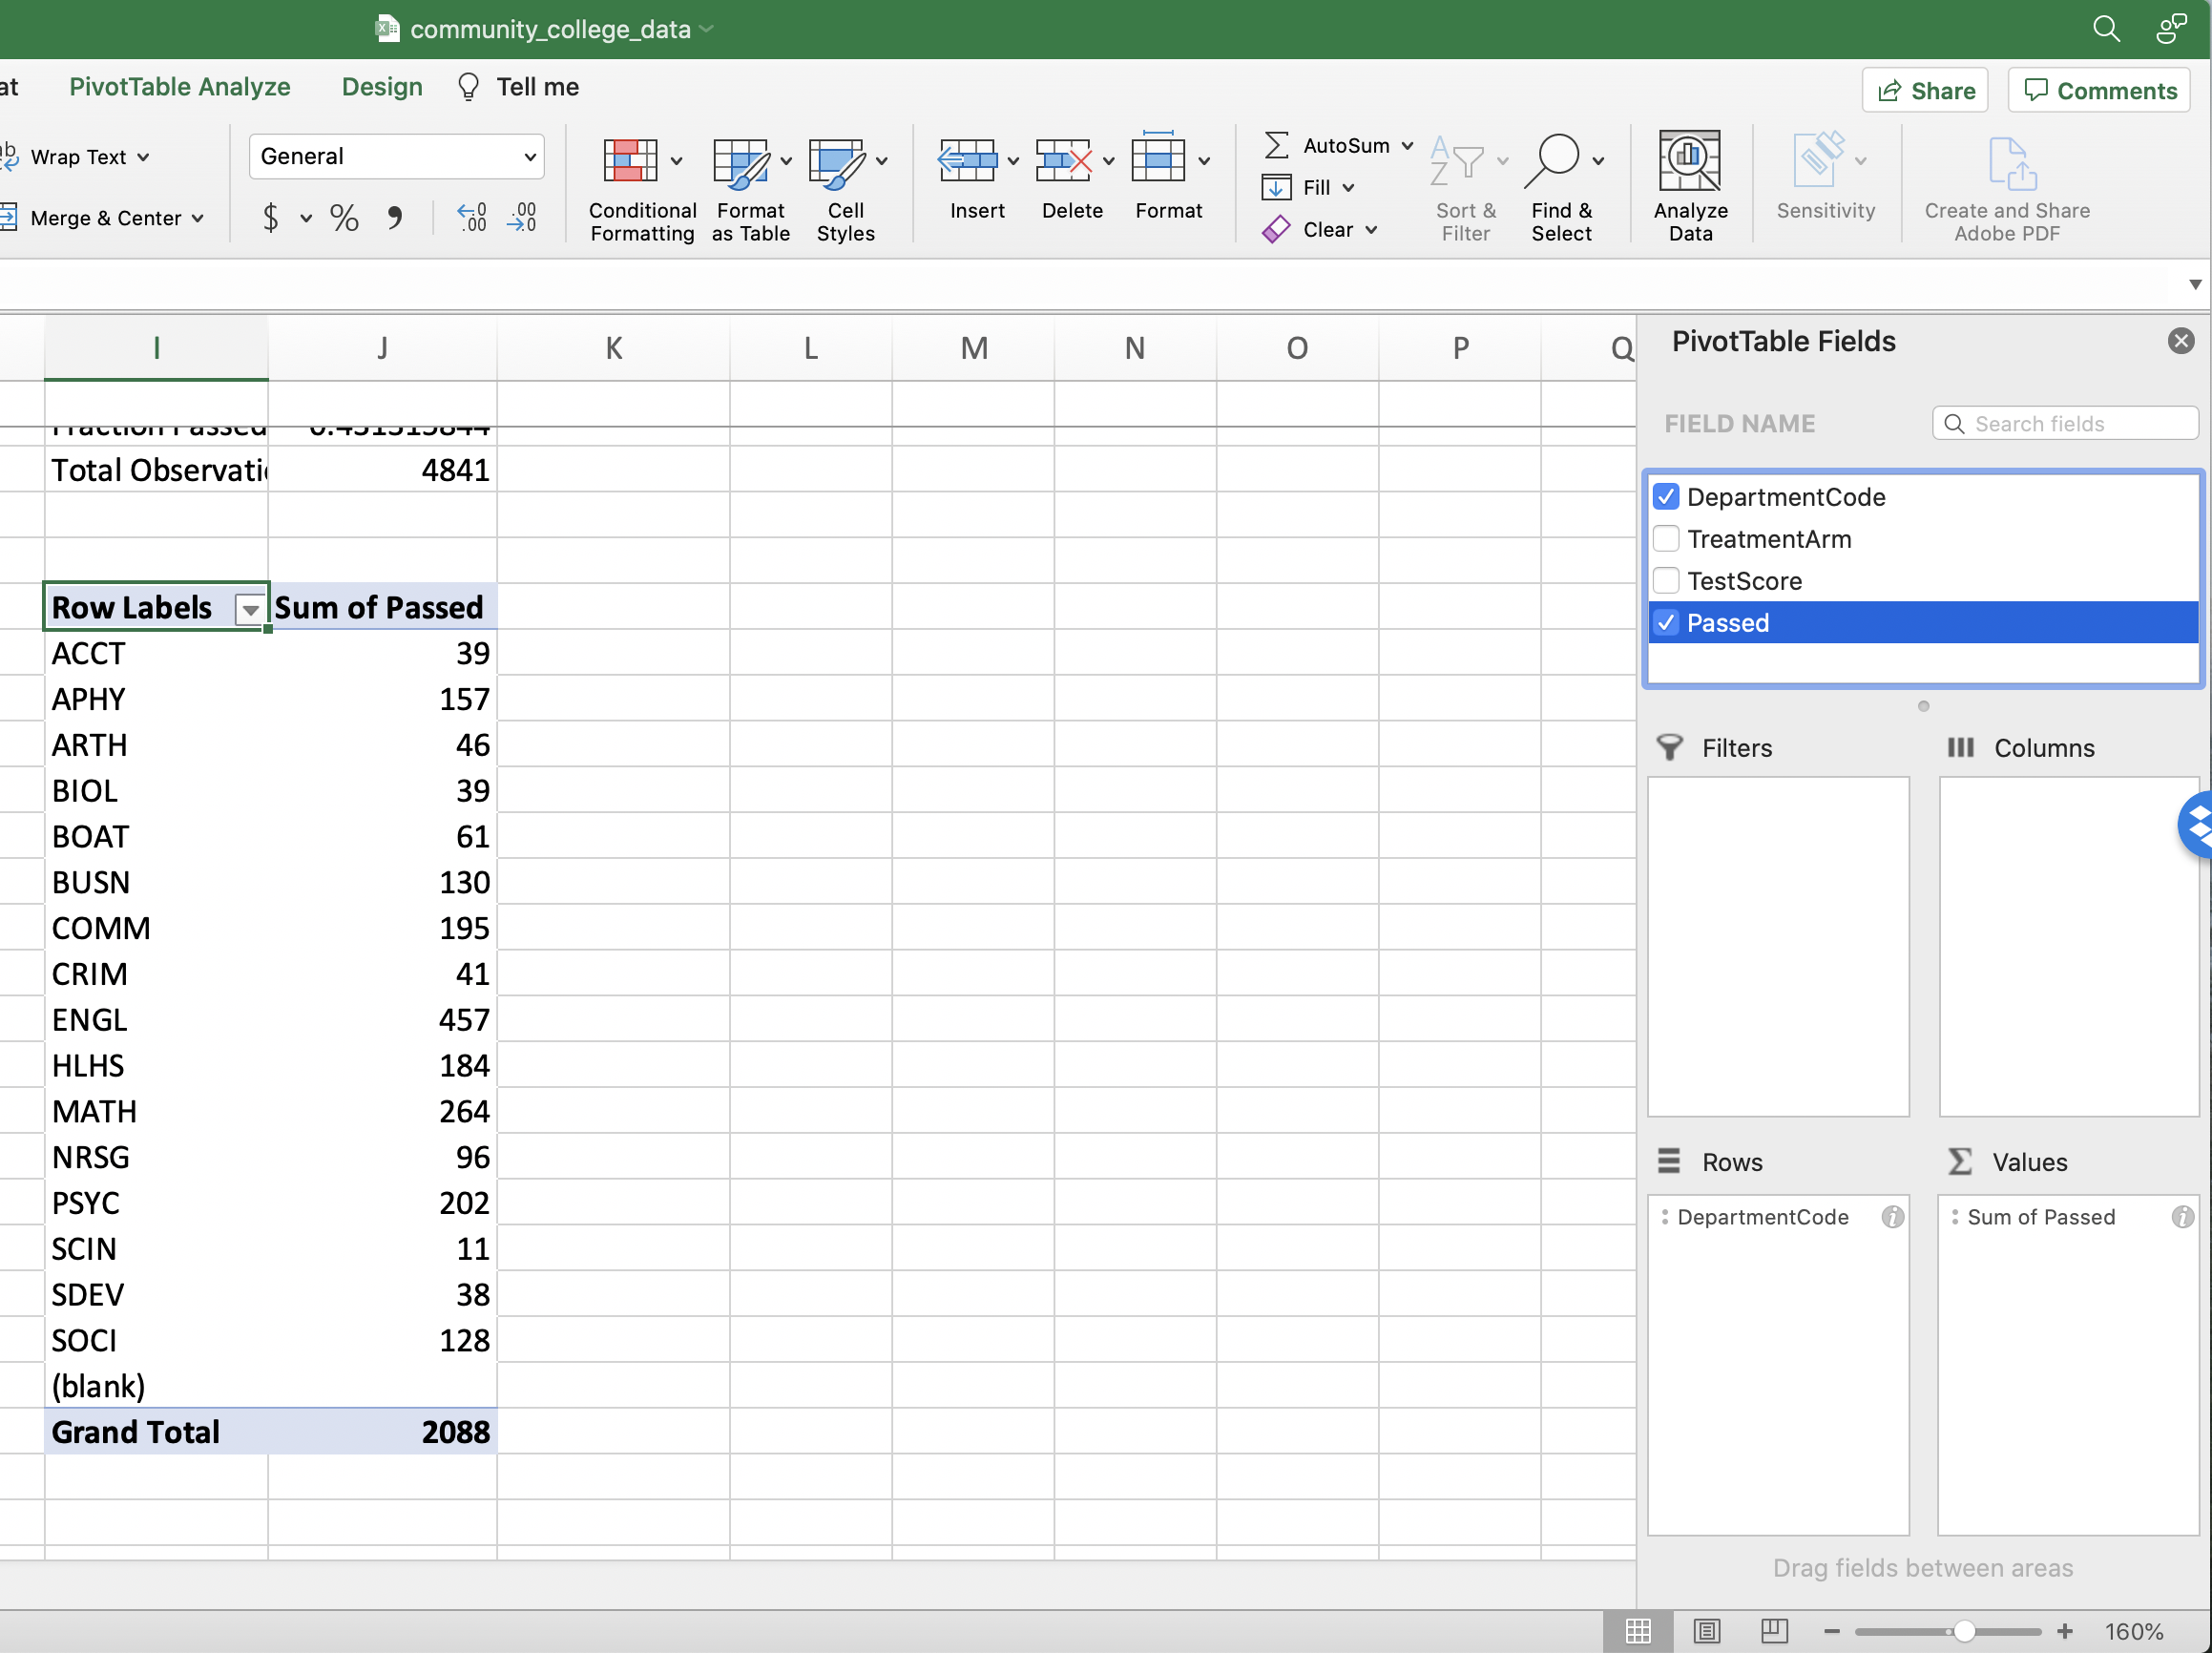
\includegraphics[width=1\linewidth]{images/01_pivot7} 

}

\caption{Average Pass Rates}\label{fig:pivot8}
\end{figure}

Now we've reached our goal! If you've followed these steps, the next table you see should be identical to Figure \ref{fig:pivotfinal}. If you found this discussion difficult to follow, I urge you to play around with pivot tables. Move variables to different panels to see how the table will change.

\section{Balance Tables}\label{balance-tables}

The key aspect of a randomized control trial that allows us to infer causality is randomization. If randomization is successful, then individuals selected for the treatment should be similar (on average) to those selected for the control. Therefore, a key component of any analysis of experimental data is to show that the treatment and control are similar based on observable characteristics.

To understand how a balance test might fail, let's imagine researchers are testing whether a given drug reduces cholesterol. The experimenters receive a list of 200 participants for the trial and decide the first 100 names on the list will receive the treatment and the second 100 will receive the placebo. What they fail to realize is that the list of applicants is sorted from youngest to oldest. Therefore, only the youngest participants receive the treatment. But younger applicants, on average, probably have lower cholesterol to begin with, so differences between treatment and control may be due to age, not due to the treatment.

If we perform a balance test (i.e.~calculate average age by treatment and control) we would immediately detect our error. Now, no ``real'' experiment would ever be run in such a way. To do so would be ignoring standard protocol for well-run experiments! Still, it is important to understand whether there are differences between treated and control units before proceeding with the main analysis. Finding persistent differences with respect to observables could be evidence that randomization somehow failed. In our empirical application, we have information on the age of the student, so let's see if age varies between the treatment and control.

We want to retrieve the average age by Treatment Arm. To do so we can use a pivot table! The \textbf{Rows} will be the Treatment Arm, while the \textbf{Values} will be age. We can follow the exact same steps as in Section \ref{S:pivottables} to build the balance table displayed in Figure \ref{fig:balance}

\begin{figure}

{\centering 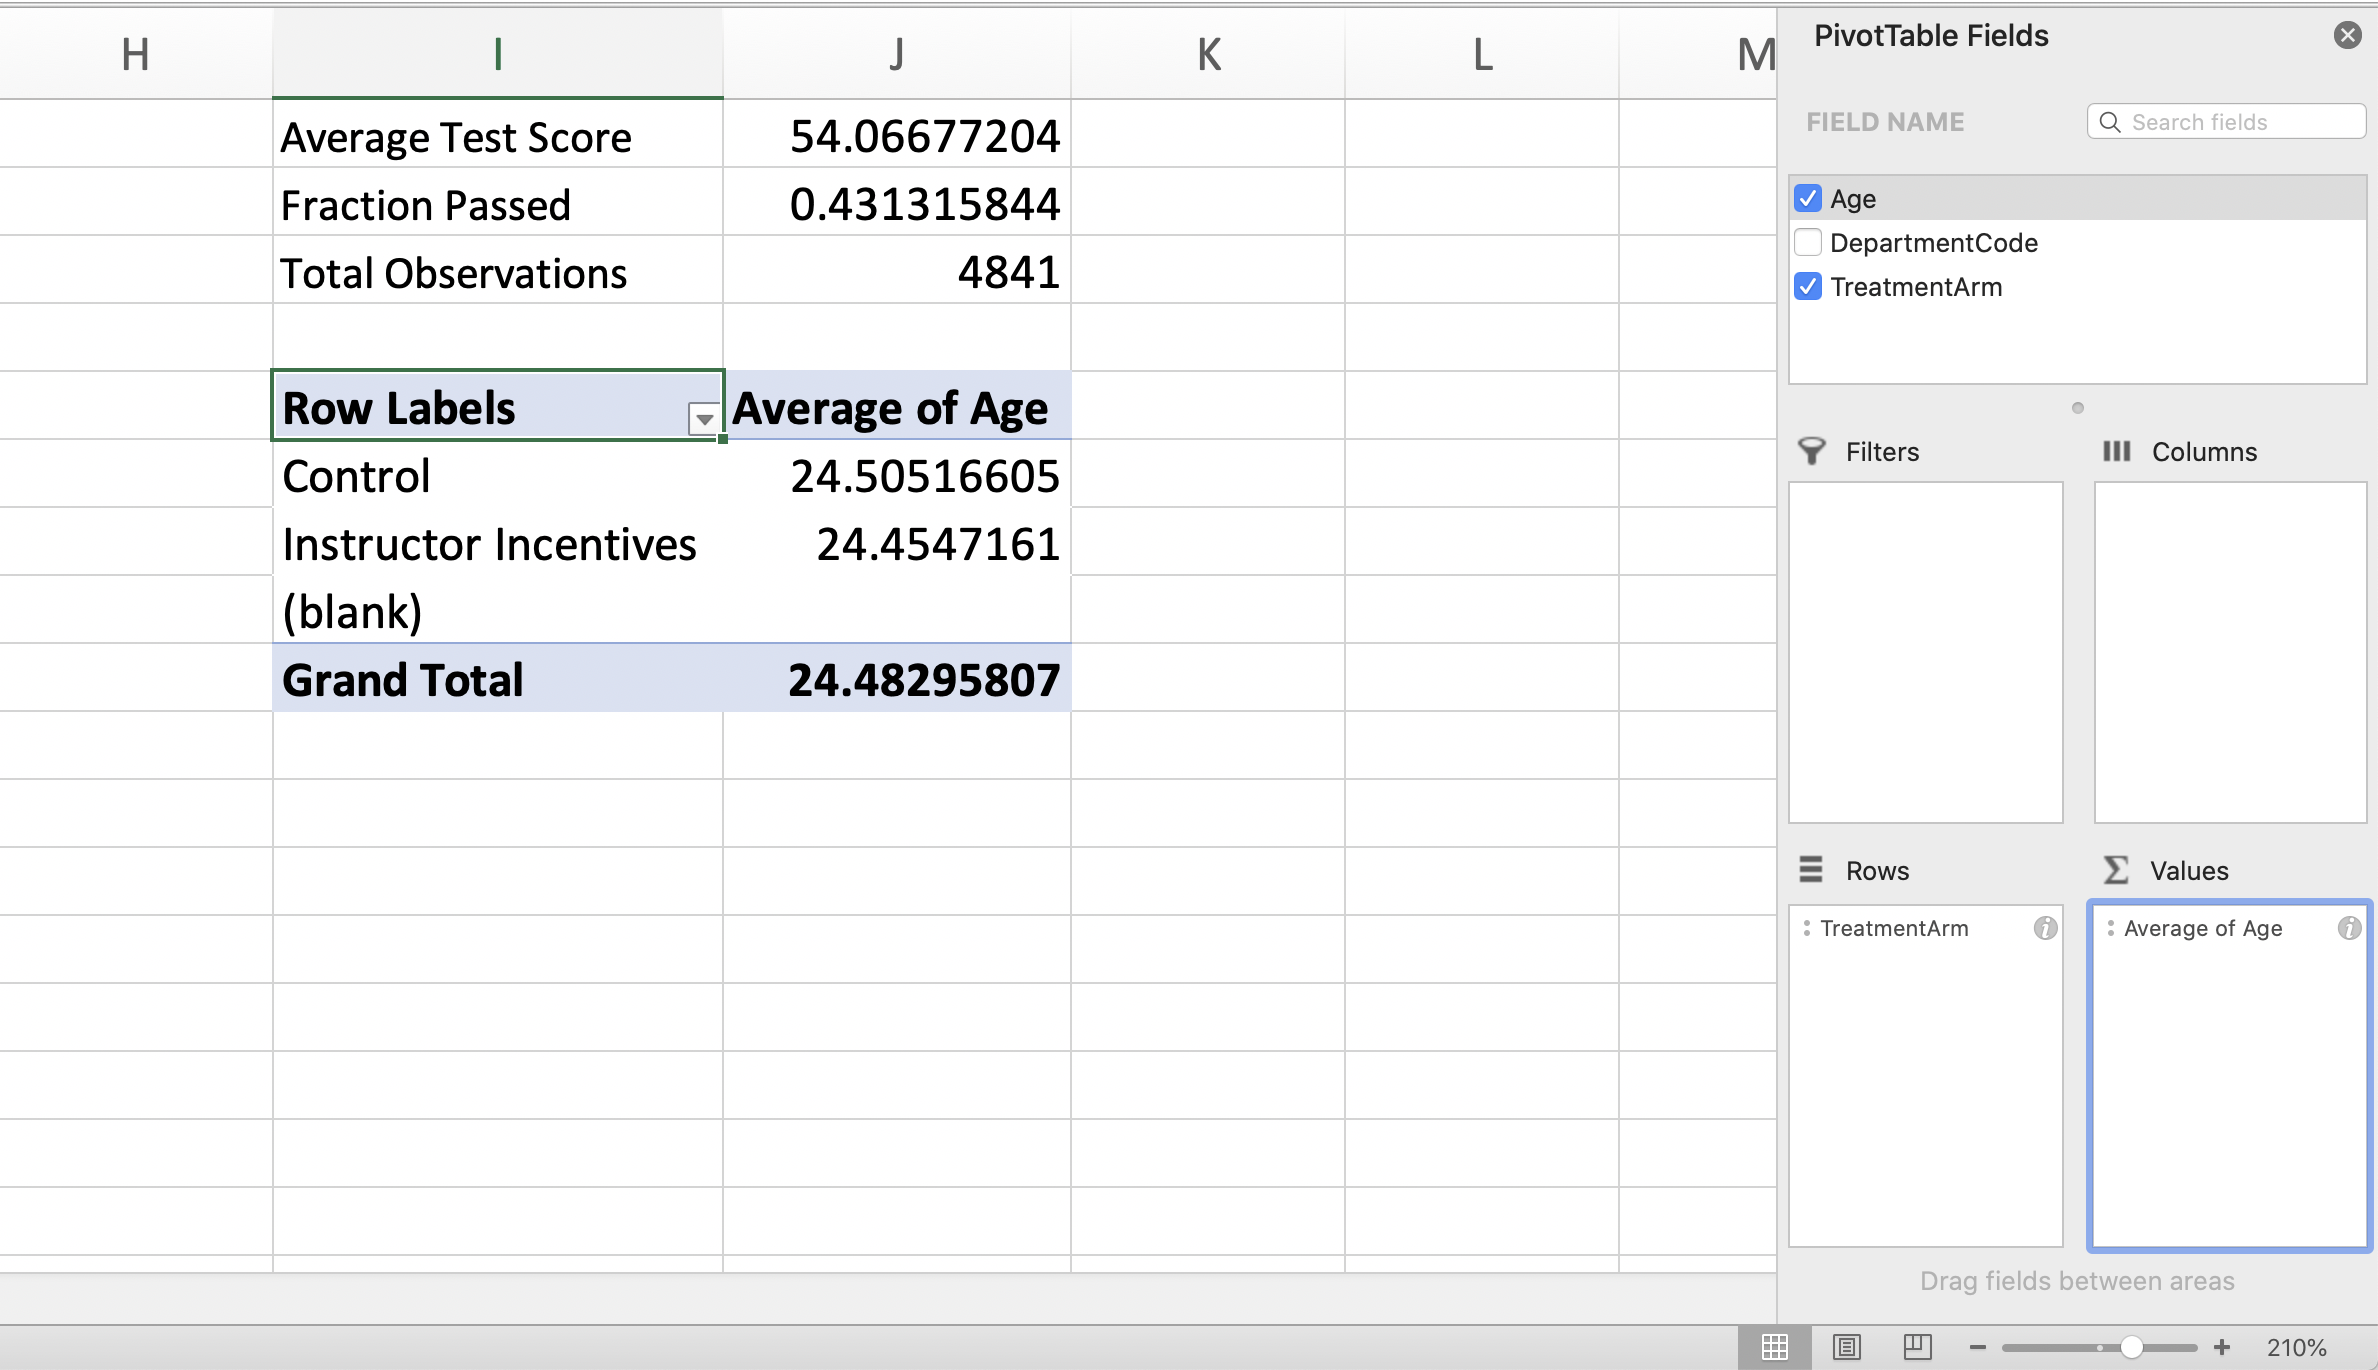
\includegraphics[width=1\linewidth]{images/01_age} 

}

\caption{Average Age by Treatment Group}\label{fig:balance}
\end{figure}

As can be seen in Figure \ref{fig:balance}, the average age in the treatment group (i.e.~the Instructor Incentives group) and the control group is roughly the same, at 24.5 years of age. While we are keeping this illustrative example simple, generally papers will show a balance table for many observables. While there may occasionally be differences between certain characteristics, on average, the two groups will tend to be similar if randomization was implemented successfully.

\section{Impact of Financial Incentives}\label{S:impact}

Now that we have checked that randomization was successful, let's estimate our first result. As a reminder, we are studying whether offering financial incentives to instructors (a 50-dollar bonus for a student passing a test) improves the performance of the students. Given only 40 percent of community college students earn a college degree within 6 years (Shapiro et al.~2017), it is important to consider tools to improve performance.

We want to compute the average pass rate for individuals in the treatment vs.~individuals in the control. We can again use a pivot table to accomplish this! Our \textbf{Rows} will be \texttt{TreatmentArm} and the \textbf{Values} will be \texttt{Passed}. Again, we can follow the steps in Section \ref{S:pivottables} to construct this table. The pivot table is displayed in Figure \ref{fig:firstresult}.

\begin{figure}

{\centering 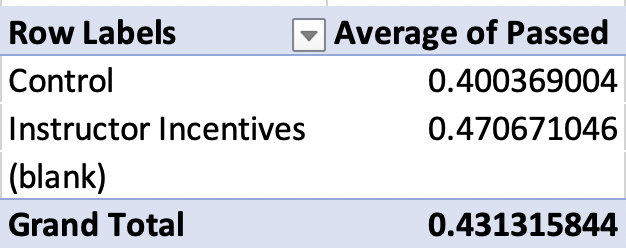
\includegraphics[width=0.5\linewidth]{images/01_result1} 

}

\caption{Impact of Financial Incentives on Pass Rates}\label{fig:firstresult}
\end{figure}

Giving instructors incentives increases pass rates by 7 percentage points. That is a big impact! Before exploring this result further, now is a good time to discuss how we accurately discuss this result. One common mistake (for both students and journalists) is to mix up the terms percentage point and percent.

In our example, 40 percent of control students pass the test, while 47 percent of treated students pass the test. Therefore, treatment increased pass rates by 7 \textbf{percentage points}. We use the term percentage points when we are comparing two percents or two rates. \textbf{The terms percentage point and percent are not interchangeable}.

How would we accurately use the term percent here to compare 40 and 47 percent? To calculate the percent increase in pass rates for the treatment relative to the control we can compute:

\[
\frac{\text{Pass Rate Treatment}-\text{Pass Rate Control}}{\text{Pass Rate Control}}= \frac{0.471-0.400}{0.400}=0.1775
\]

So the treatment pass rate is 17.75 percent higher relative to the control. This mistake can be misleading! For example, let's imagine the probability of dying during a given procedure is 2 percent. However, a doctor tries a new surgical technique and finds the probability of dying under the alternative procedure is 1 percent.

This is a 1 percentage point decrease in the probability of dying during the procedure. However, it is a 50 percent decrease in the probability of dying during the procedure. Now, if a journalist wrote an article and incorrectly stated that the new procedure decreases death rates by 1 percent, then it sounds as if the new technique is not that much better than the old technique. However, that is the wrong conclusion. The correct conclusion is that a 1 percentage point decrease in the probability of dying implies a 50 percent reduction in the probability of dying, a huge advance!

So let's take stock of what we have learned. Providing financial incentives to community college instructors seems to increase pass rates on average. This is an important finding. Prior work on ``pay-for-performance'' in the United States has shown limited effectiveness in K-12 schools (See Neal (2011)). But this is the first study to show financial incentives can be an effective tool in the Community College setting. This is an important general lesson: the context of the treatment matters. Just because a treatment is effective in one setting doesn't mean it will be effective in another (or vice-versa).

Next, let's talk about what else we can learn from this experiment. Well, this study was done across many different subjects. Maybe the effect of financial incentives differs depending on the department. It may be easier to get students over the pass threshold in some disciplines, making the incentives potentially more effective.

To explore this question we can adjust our pivot table a bit. We will proceed in two steps:

\begin{itemize}
\item
  First: Move ``TreatmentArm'' to Column Panel
\item
  Second: Move ``DepartmentCode'' to Row
\end{itemize}

If you have successfully moved the variables around, your PivotTable Fields should look like \ref{fig:pivotfield}.

\begin{figure}

{\centering 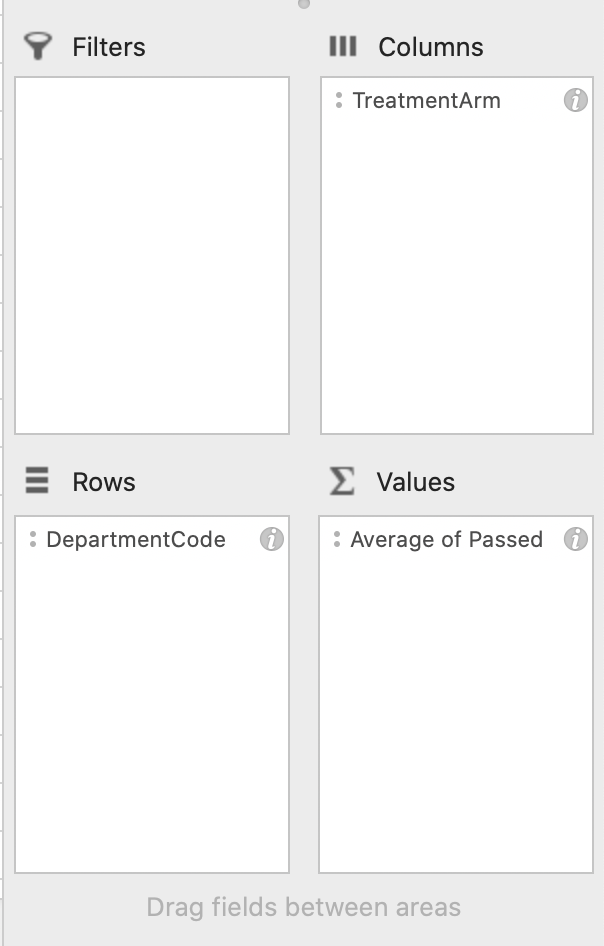
\includegraphics[width=0.35\linewidth]{images/01_pivot_field} 

}

\caption{Pivot Fields}\label{fig:pivotfield}
\end{figure}

Figure \ref{fig:hetresults} displays the results.

\begin{figure}

{\centering 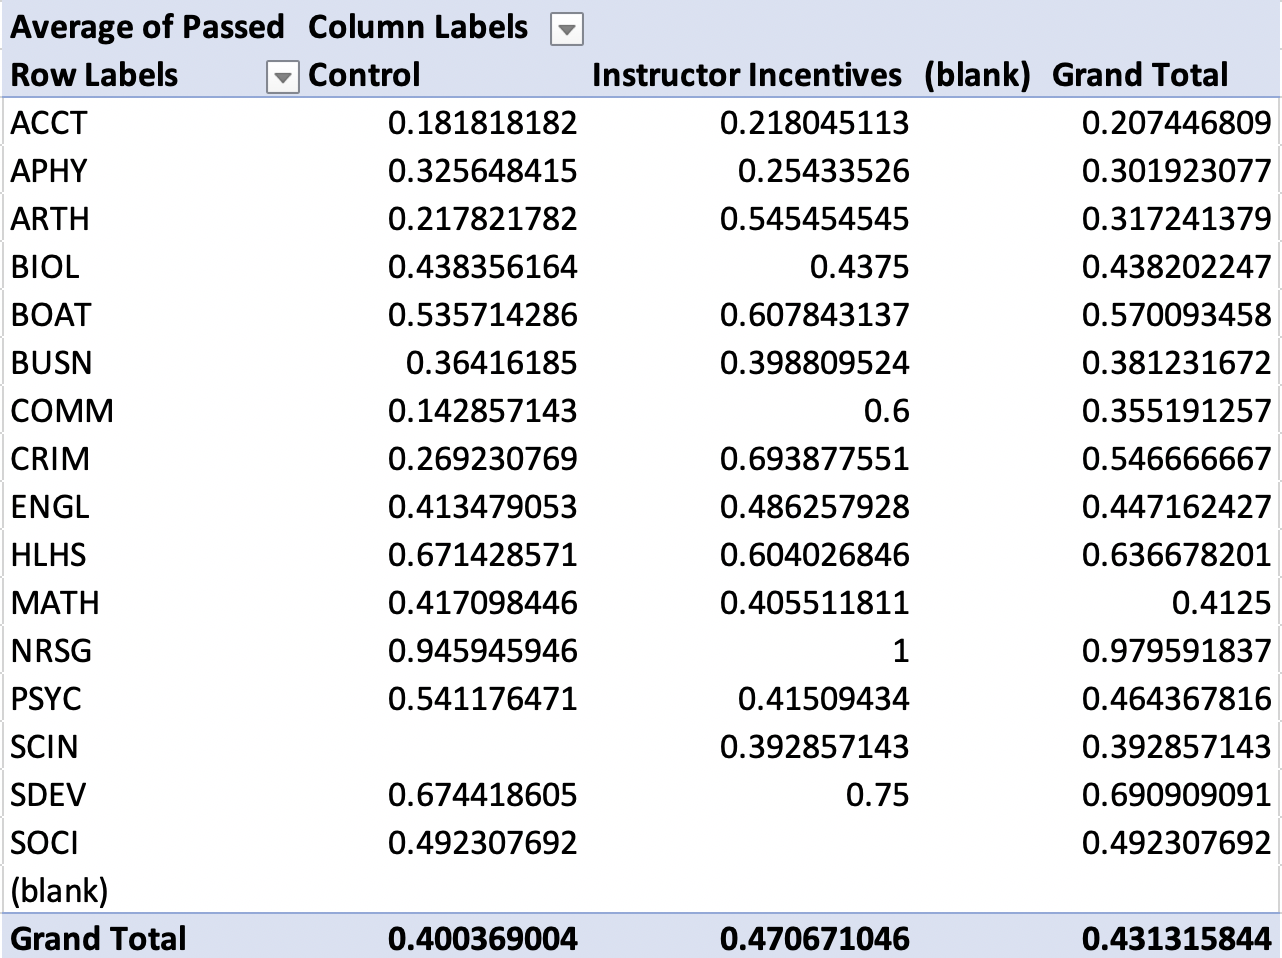
\includegraphics[width=0.75\linewidth]{images/01_pivot_het_blank} 

}

\caption{Pivot Table Showing Pass Rates by Treatment and Control Across Departments}\label{fig:hetresults}
\end{figure}

In some departments, the instructor incentives were incredibly effective. For example, in the communications department (\texttt{COMM}), the instructor incentives led to a dramatic increase in pass rates. In the control group, the pass rates were only 14 percent, while they were 60 percent in the treatment group. This is a 46 percentage point increase in pass rates, or equivalently, a 329 percent increase in pass rates in the treatment relative to the control

In other departments, however, the instructor incentives don't seem particularly effective. For example, in the math department (\texttt{MATH}), pass rates were similar in both the treatment group (41 percent) and the control group (42 percent). Therefore, it does not seem as if these incentives impact all departments in the same way.

It is often useful to explore heterogeneity in this way. Through this analysis, we learned financial incentives are not necessarily a ``one-size fits all'' solution. Some departments can increase pass rates considerably, while others show modest or even zero/negative impact. If we want to apply these results to other settings we will need to think about how the other setting is similar or different to ours.

\section{Pivot Charts (Basic)}\label{S:pivotbasic}

In this section, we will learn about something closely related to pivot tables: a pivot chart. Pivot charts and pivot tables contain the same information, but often charts/figures are more effective in presenting information. In popular press articles, it's common to see a nicely designed figure to grab readers' attention.

Let's walk through how to make a pivot chart in Excel. To insert a pivot chart, go to the Insert tab and click the Pivot Chart icon

\begin{figure}

{\centering 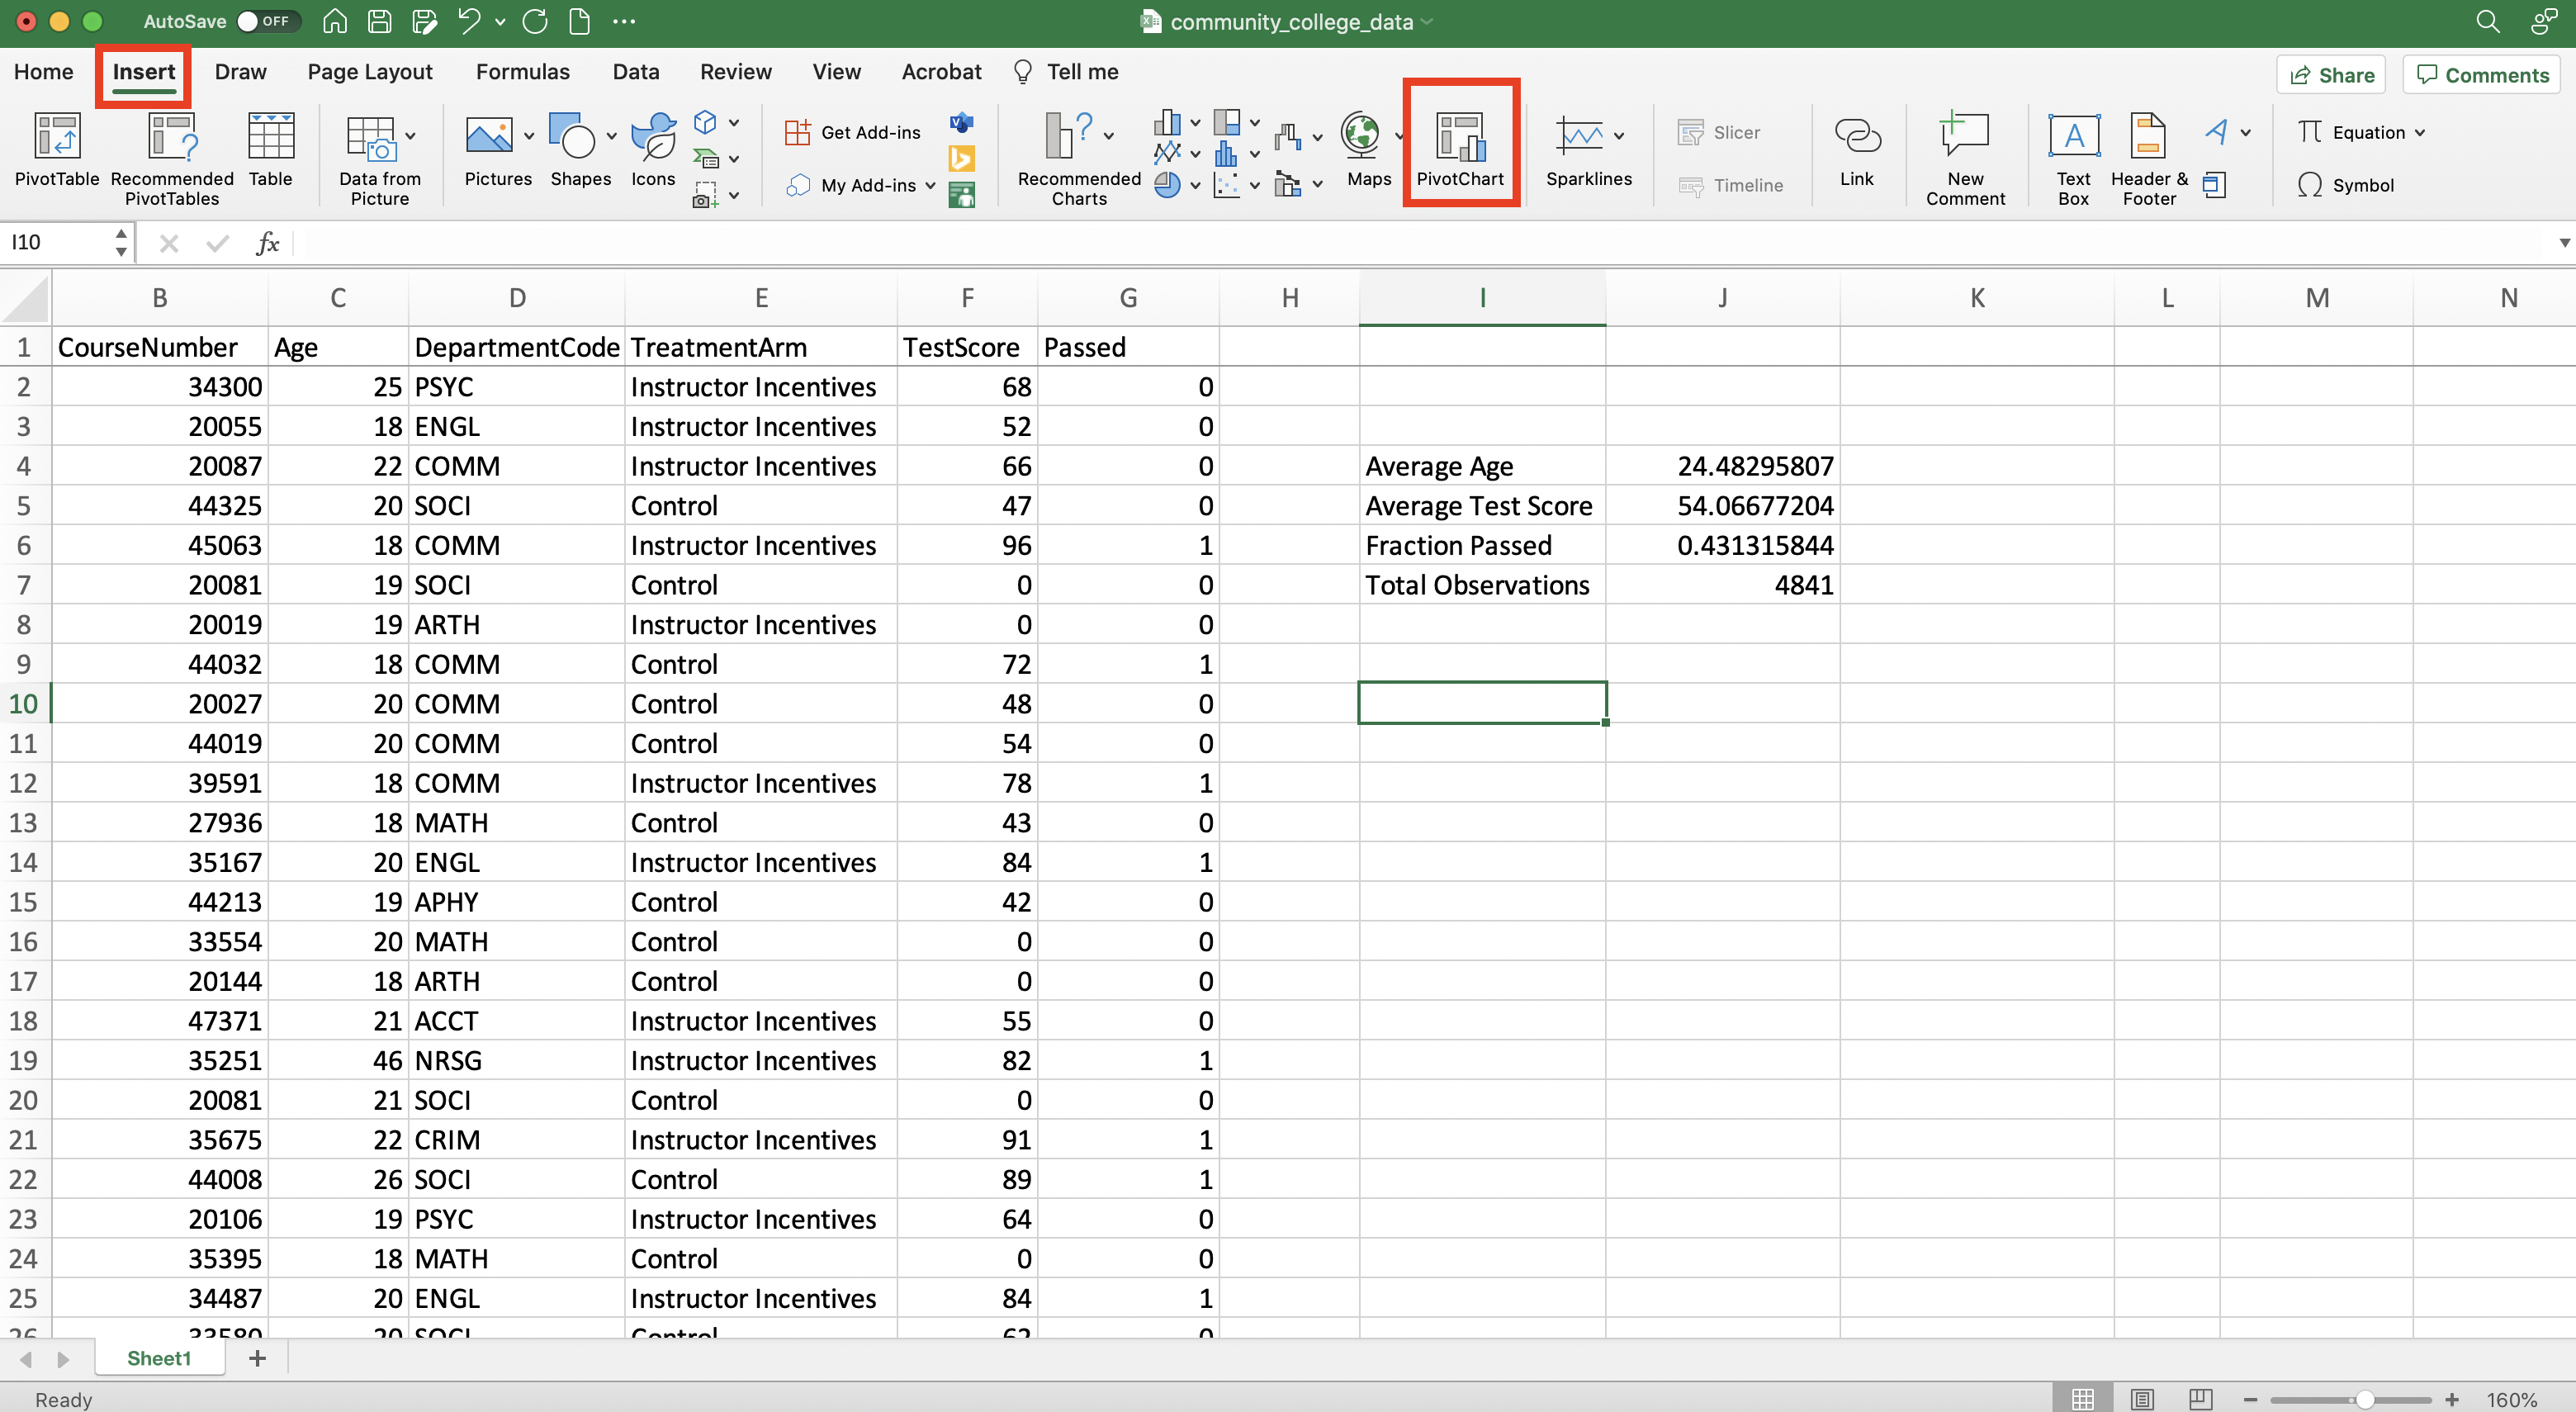
\includegraphics[width=1\linewidth]{images/01_pivot_chart1} 

}

\caption{Inserting a Pivot Chart}\label{fig:pivotchart1}
\end{figure}

The pivot chart fields are similar to the pivot table fields. We can choose different combinations to create different figures

\begin{figure}

{\centering 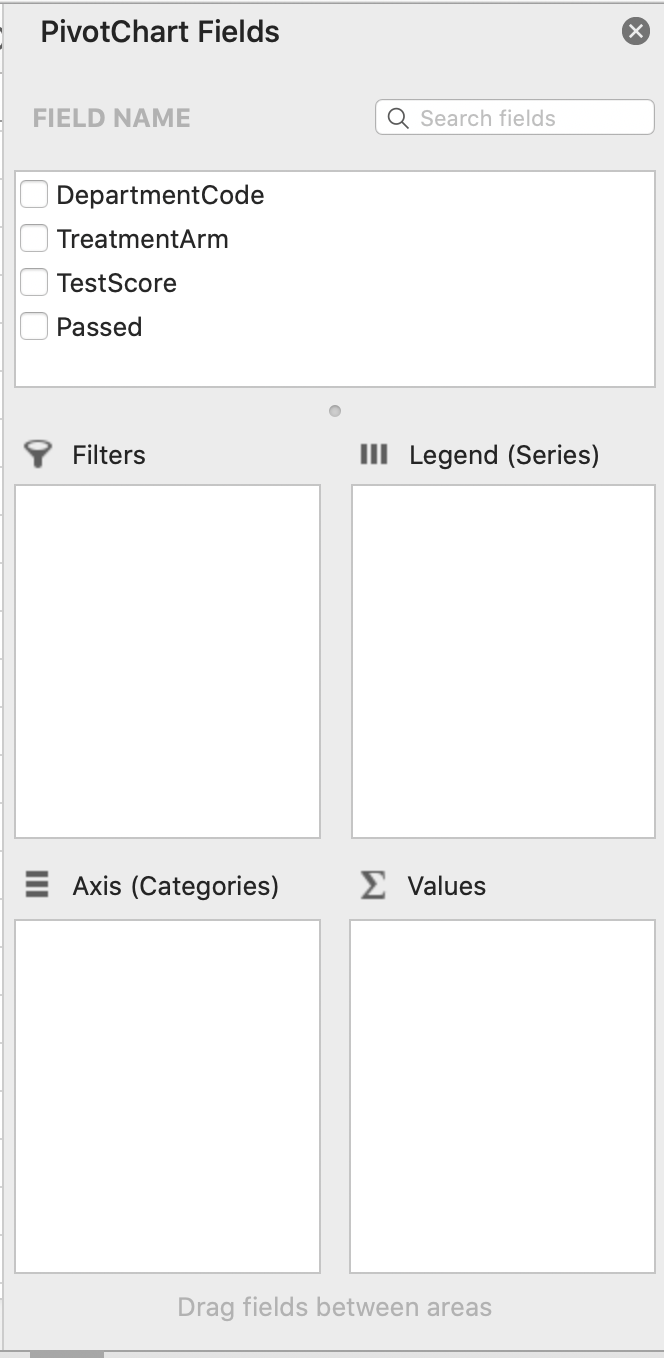
\includegraphics[width=0.25\linewidth]{images/01_pivot_chart2} 

}

\caption{Pivot Chart Fields}\label{fig:pivotchart2}
\end{figure}

Our goal now is to create a pivot chart that presents the first main result. In other words, a chart that shows average pass rates by \texttt{TreatmentArm}. Therefore, in the pivot chart fields we will put \texttt{TreatmentArm} on the Axis and \texttt{Average\ of\ Passed} as the Values.

\begin{figure}

{\centering 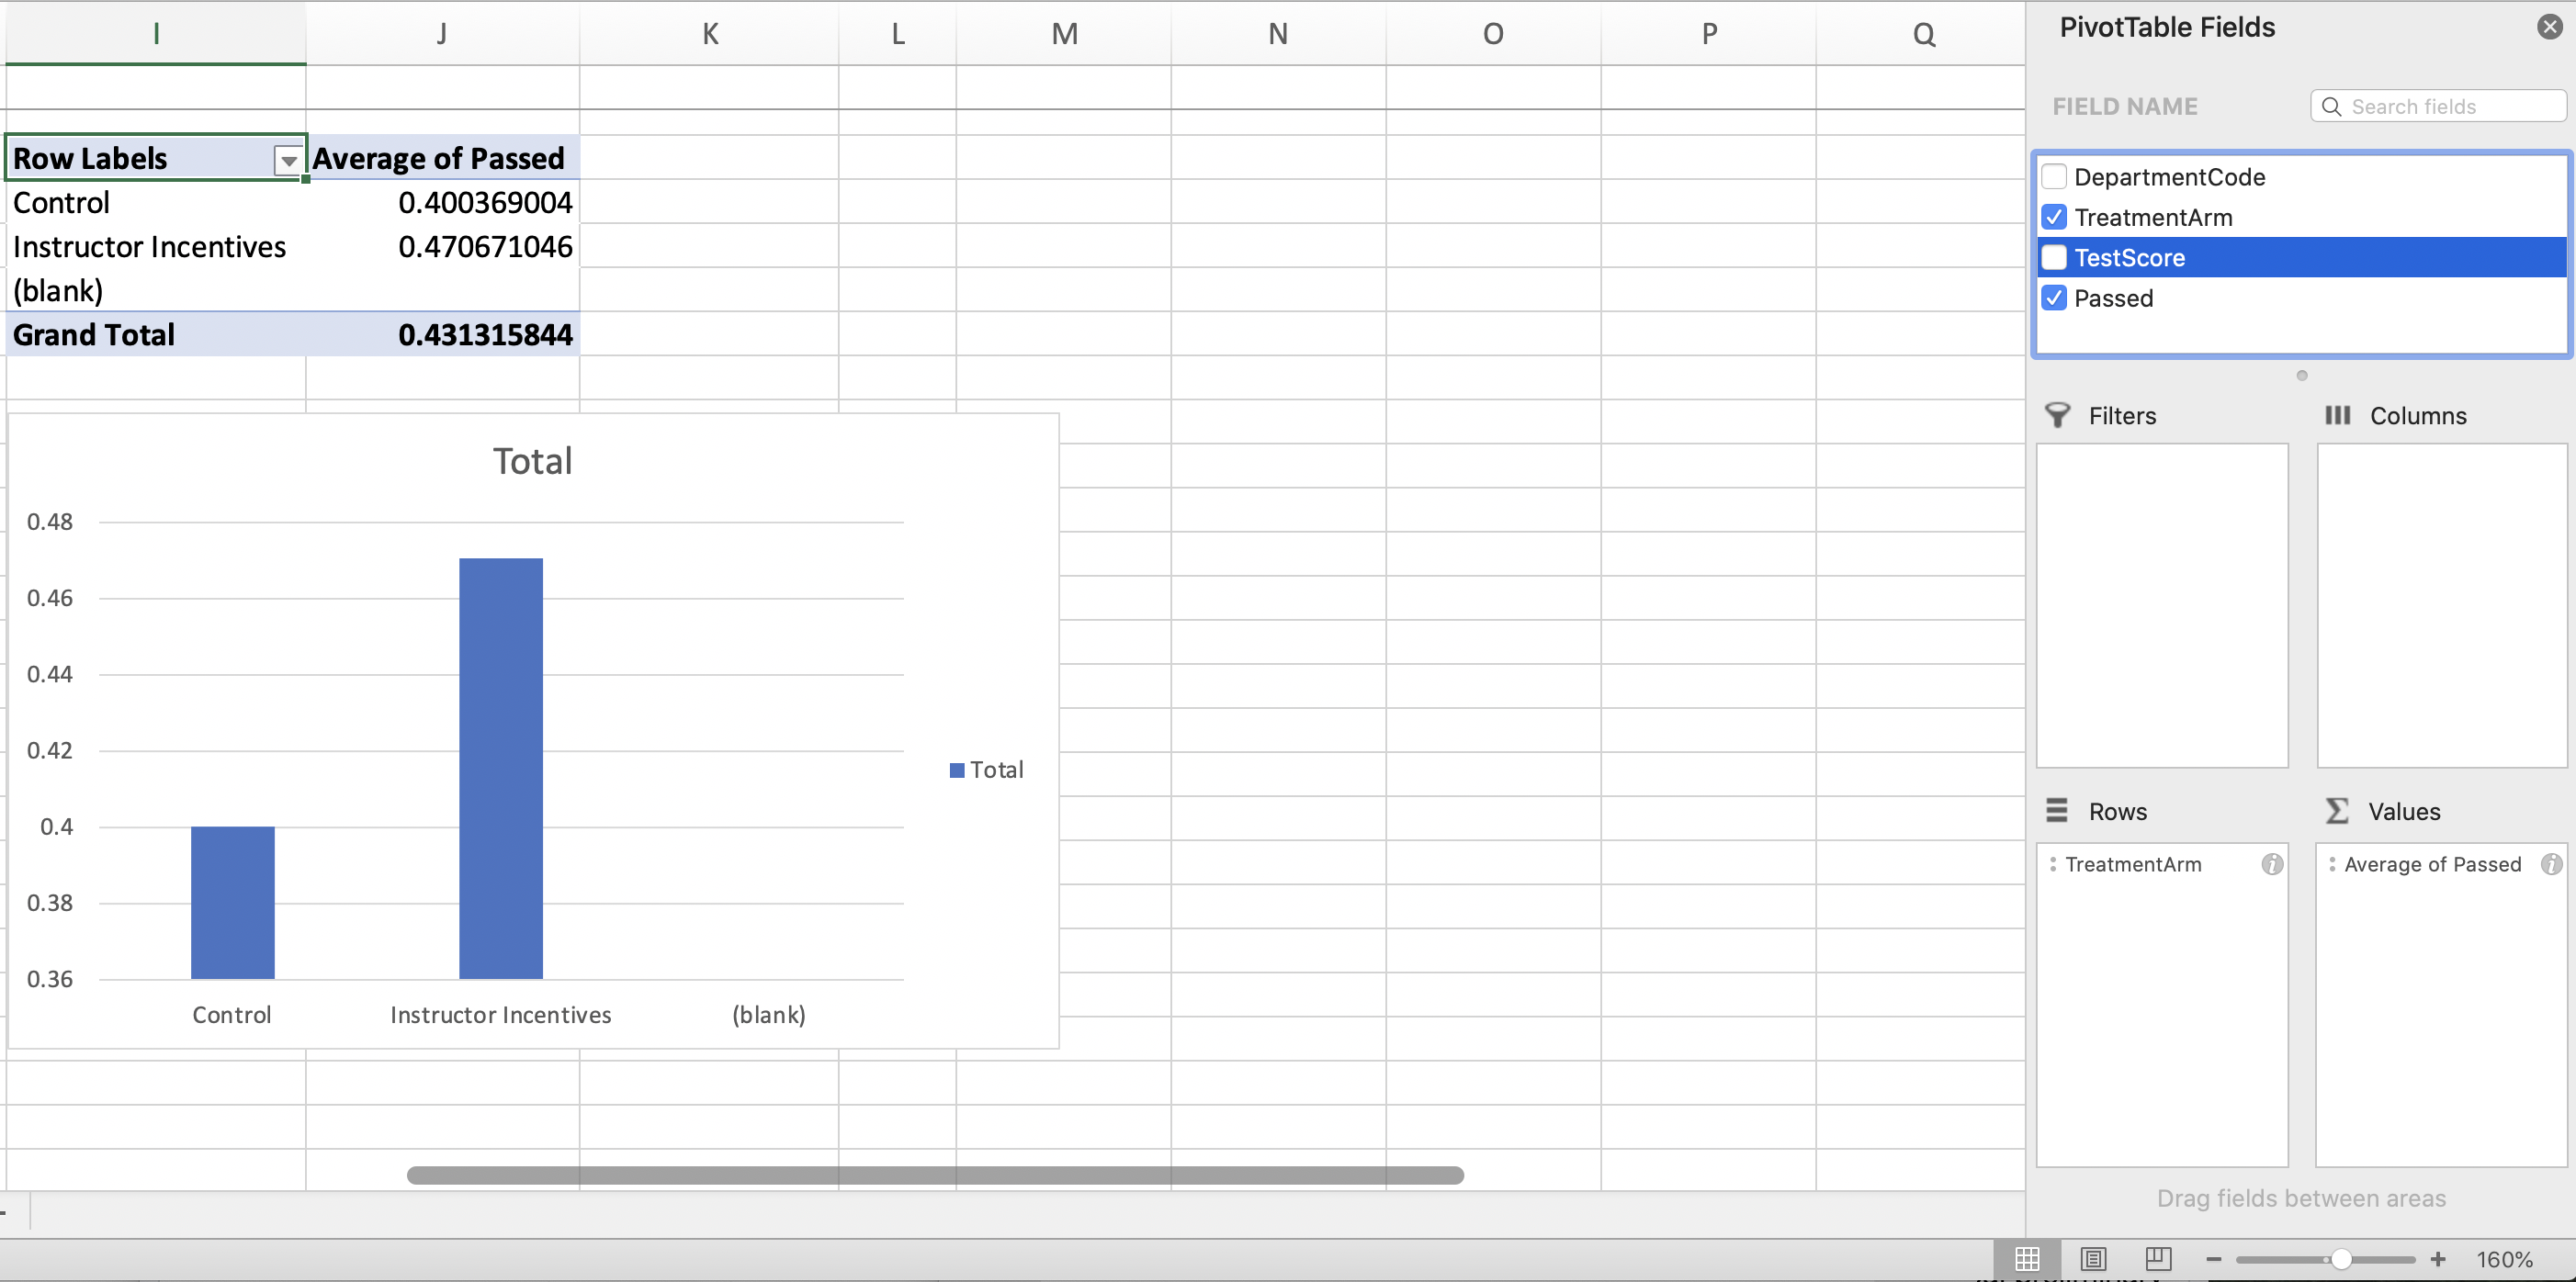
\includegraphics[width=1\linewidth]{images/01_pivot_chart3} 

}

\caption{Pivot Chart Fields}\label{fig:pivotchart3}
\end{figure}

You can see a pivot table has also been created in Figure \ref{fig:pivotchart3}. The pivot table and chart are linked (i.e.~changes made to the pivot table will be reflected in the chart).

The ``(blank)'' on the horizontal axis serves no purpose. We can rid of it by altering the pivot table. To do so we can click the arrow on the bottom right of the cell that reads ``Row Labels''

\begin{figure}

{\centering 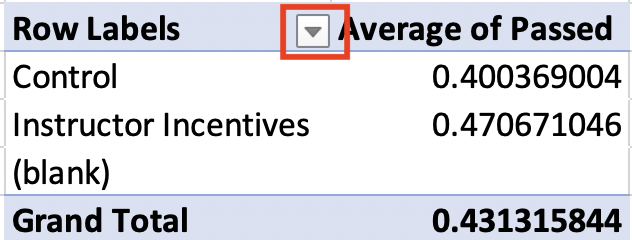
\includegraphics[width=0.5\linewidth]{images/01_pivot_chart4} 

}

\caption{Filtering Out Blank}\label{fig:pivotchart4}
\end{figure}

Next, a window will pop up. We can deselect ``(blank)'' to remove it from the Pivot Table

\begin{figure}

{\centering 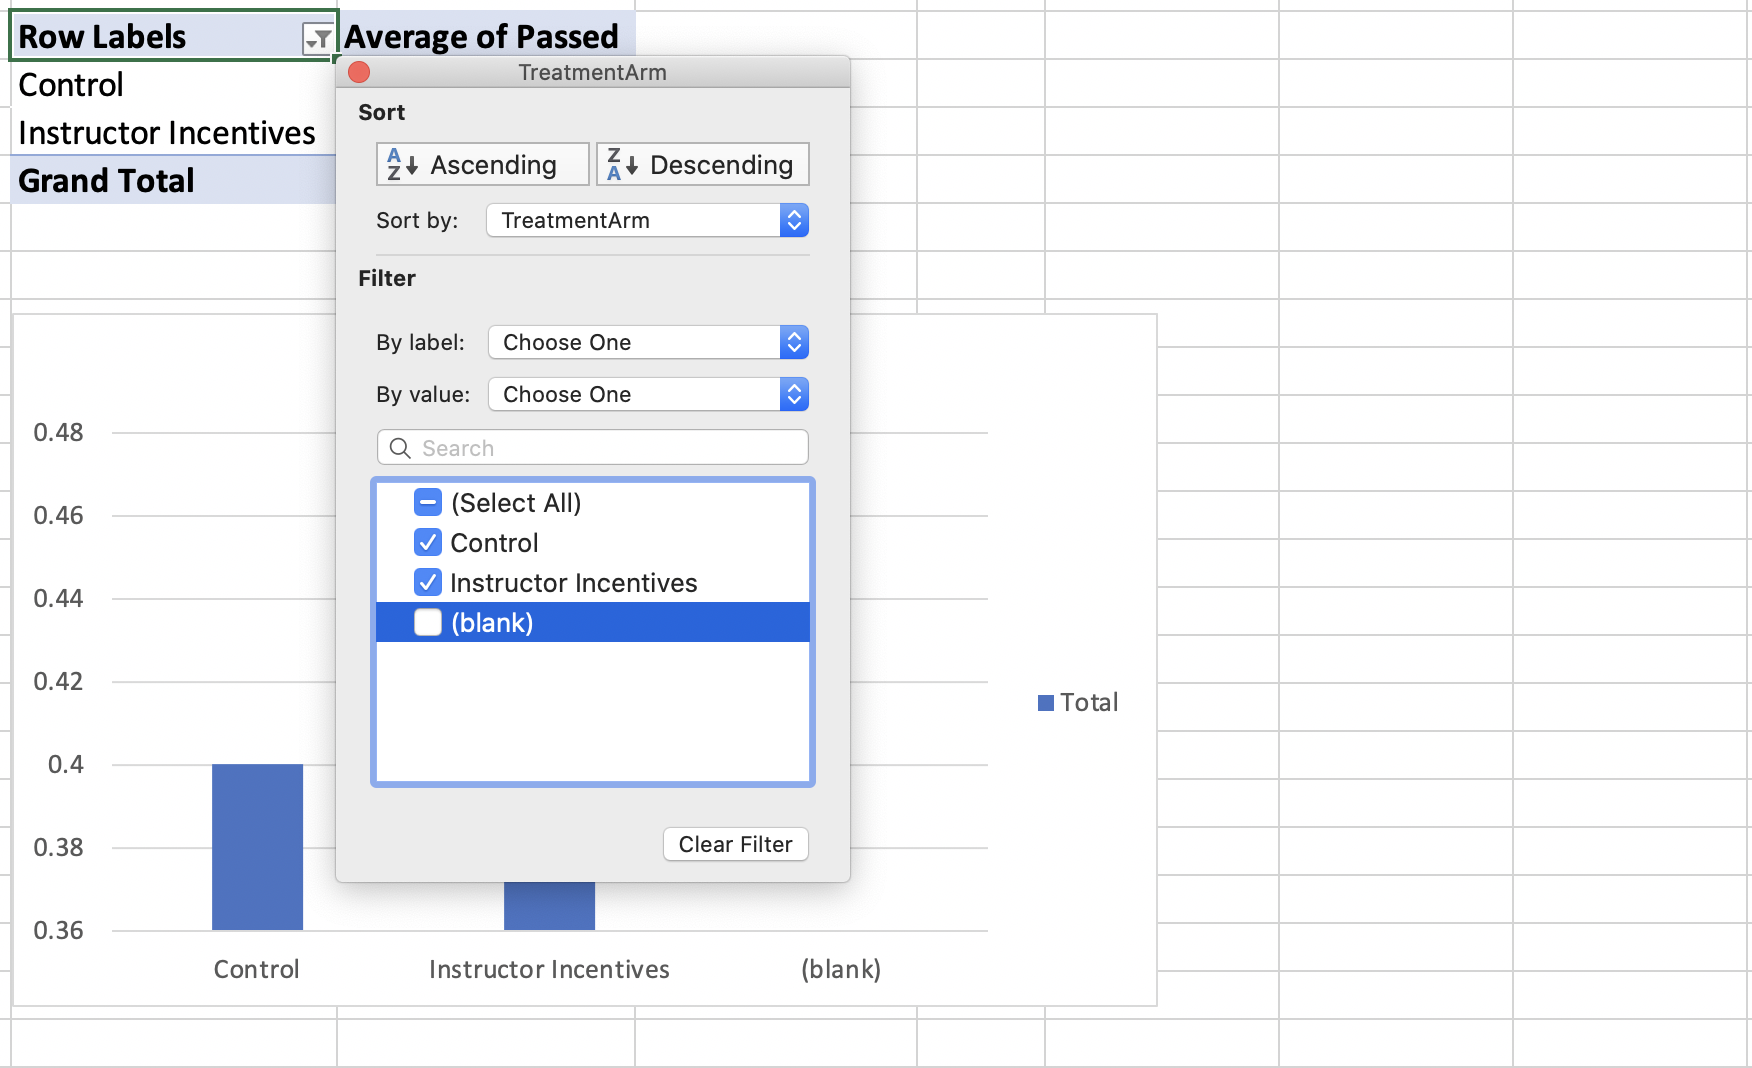
\includegraphics[width=0.7\linewidth]{images/01_pivot_chart5} 

}

\caption{Filtering Out Blank}\label{fig:pivotchart5}
\end{figure}

Blank has now been removed from both the Pivot Table and the Pivot Chart. While our current figure technically has all the relevant information to understand the impact of financial incentives on student performance, it leaves a lot to be desired. We need a reader to understand the information clearly, but right now we are missing proper titles and labels. This is something that will come up many times throughout the course. To convey our data analysis effectively, we need to ensure that figures and tables are properly titled and labeled. One ``trick'' is to pretend you have never seen the table or figure you have created. Would you be able to understand the information? If not, what is missing?

To edit the title, we can just click in the ``Total'' box at the top and edit. Make sure to always give descriptive titles with proper capitalization

\begin{figure}

{\centering 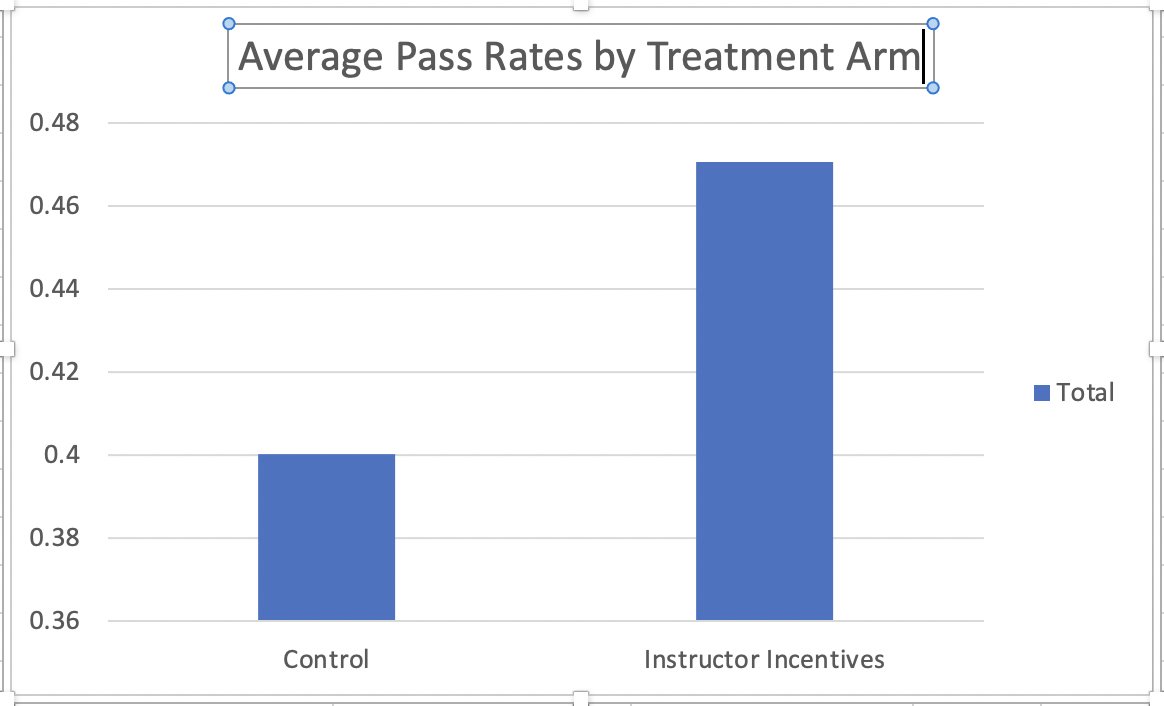
\includegraphics[width=0.7\linewidth]{images/01_pivot_chart8} 

}

\caption{Adding a Title}\label{fig:pivotchart8}
\end{figure}

We also need to add horizontal and vertical axes titles. To insert these go to ``Design'', click ``Insert Chart Element'', and select one of the Axes Titles to add in a text box that we can edit

\begin{figure}

{\centering 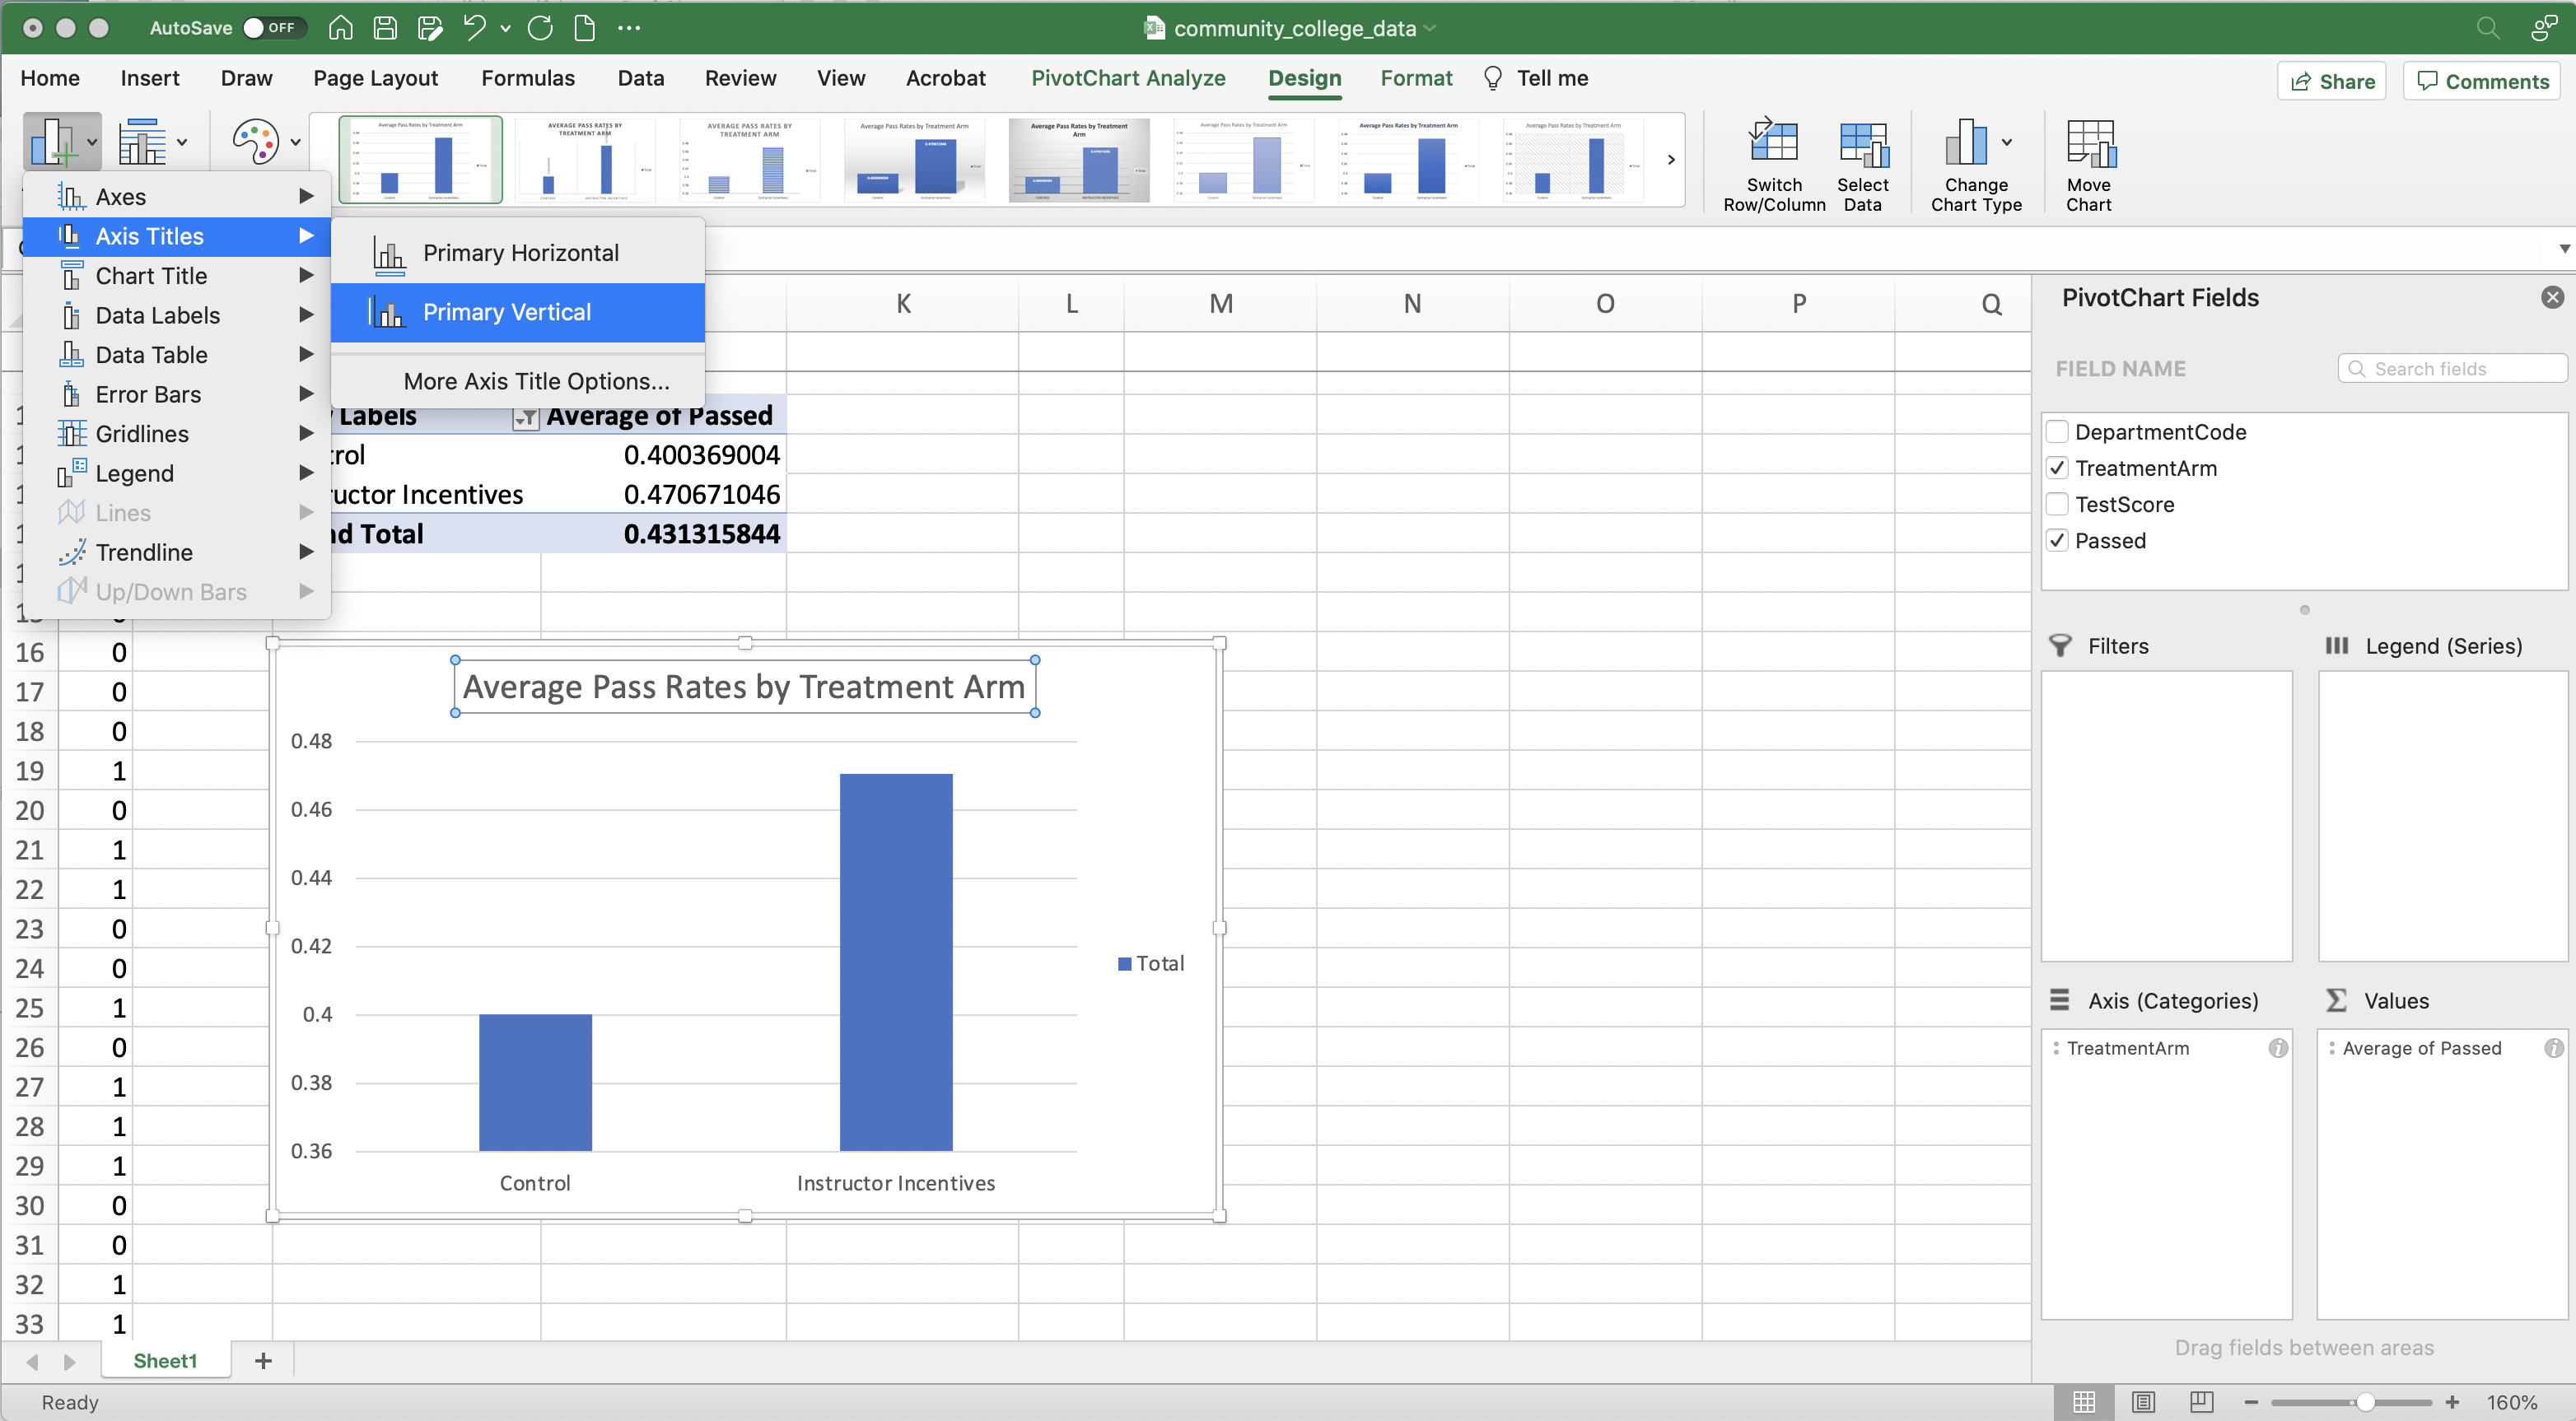
\includegraphics[width=0.9\linewidth]{images/01_pivot_chart9} 

}

\caption{Adding Axes Titles}\label{fig:pivotchart9}
\end{figure}

Once we have added in proper axes titles, there is just one last thing to do. Our figure has a legend on the right, but it is neither descriptive nor necessary in this particular figure. Legends are important when you are trying to differentiate between the bars in a bar chart. For our figure, we can already discern this from the horizontal axes labels. Therefore, we can simply click on the legend and press backspace to delete it. Finally, we have our ultimate figure that shows average pass rates by \texttt{TreatmentArm}

\begin{figure}

{\centering 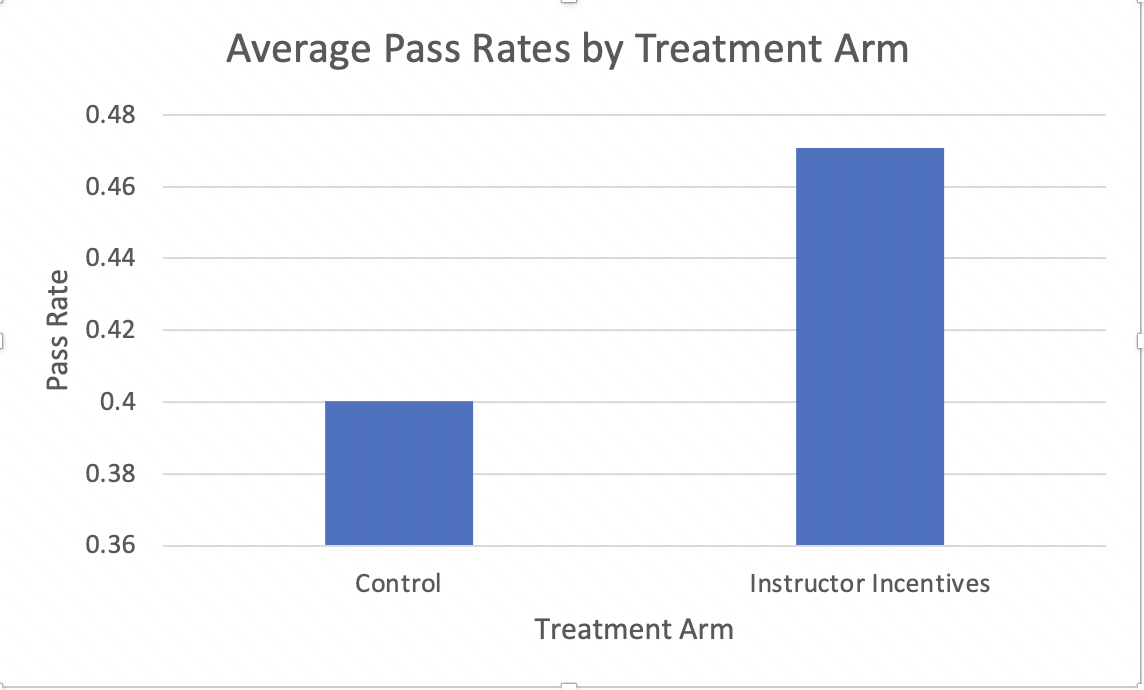
\includegraphics[width=0.6\linewidth]{images/01_pivot_chart11} 

}

\caption{Average Pass Rates by Treatment Arm}\label{fig:pivotchart11}
\end{figure}

\section{Pivot Charts (Advanced)}\label{S:pivotadvanced}

Next, we are going to use pivot charts to display the heterogeneity in treatment effects across different departments. Our pivot chart currently displays the average of \texttt{Passed} by \texttt{TreatmentArm}. We want to present the average of \texttt{Passed} by \texttt{TreatmentArm} separately for every value of \texttt{DepartmentCode}.

Therefore, we need to place \texttt{DepartmentCode} somewhere in our Pivot Chart Fields. But where? Legend(Series) seems like a potentially good choice. Whatever variable you put into Legend(Series), Excel will create a plot similar to the current plot, but with separate bars for every value of the variable in Legend(Series). In our case, separate bar charts for every value of \texttt{DepartmentCode}

Figure \ref{fig:advpivot2} displays the results if we drag \texttt{DepartmentCode} to Legend(Series).

\begin{figure}

{\centering 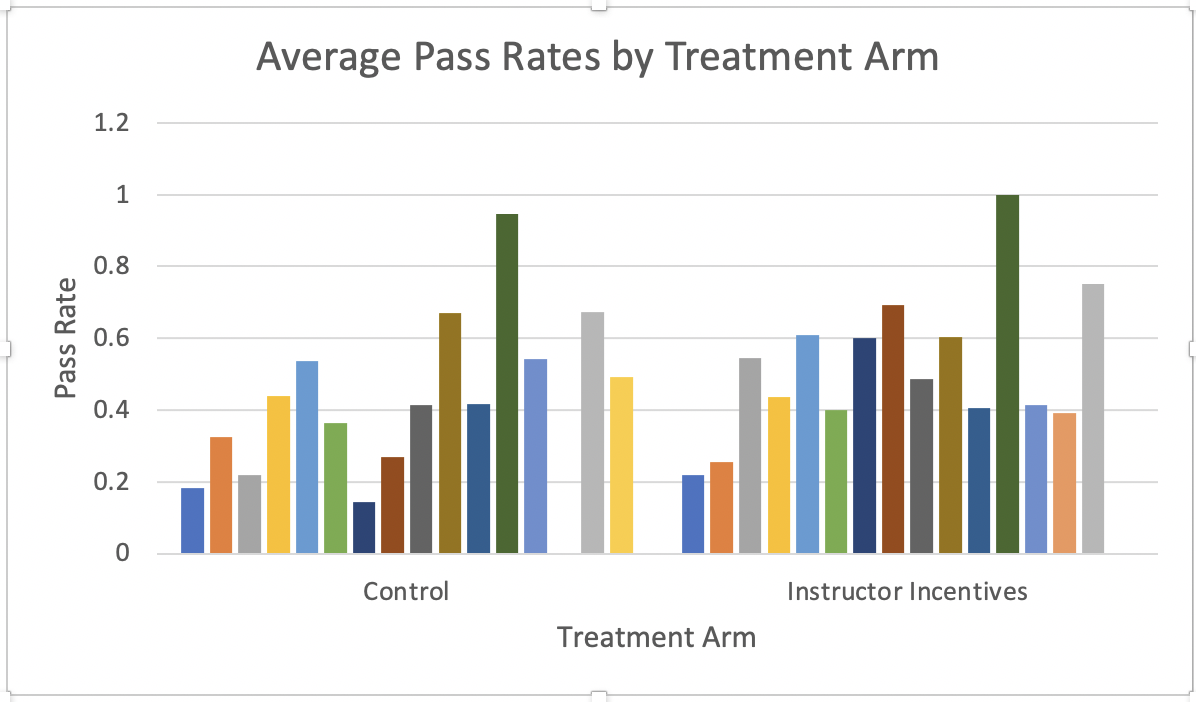
\includegraphics[width=0.6\linewidth]{images/01_adv_pivot2} 

}

\caption{Average Pass Rates by Treatment Arm and Department}\label{fig:advpivot2}
\end{figure}

Here would be a good time to check whether this figure is interpretable for someone who did not create it. Right now, it is unclear what the different bars represent. There is no legend that shows which color bar is associated with which department.

To insert a Legend, go to ``Design'', press ``Add Chart Element'' and navigate to ``Legend''

\begin{figure}

{\centering 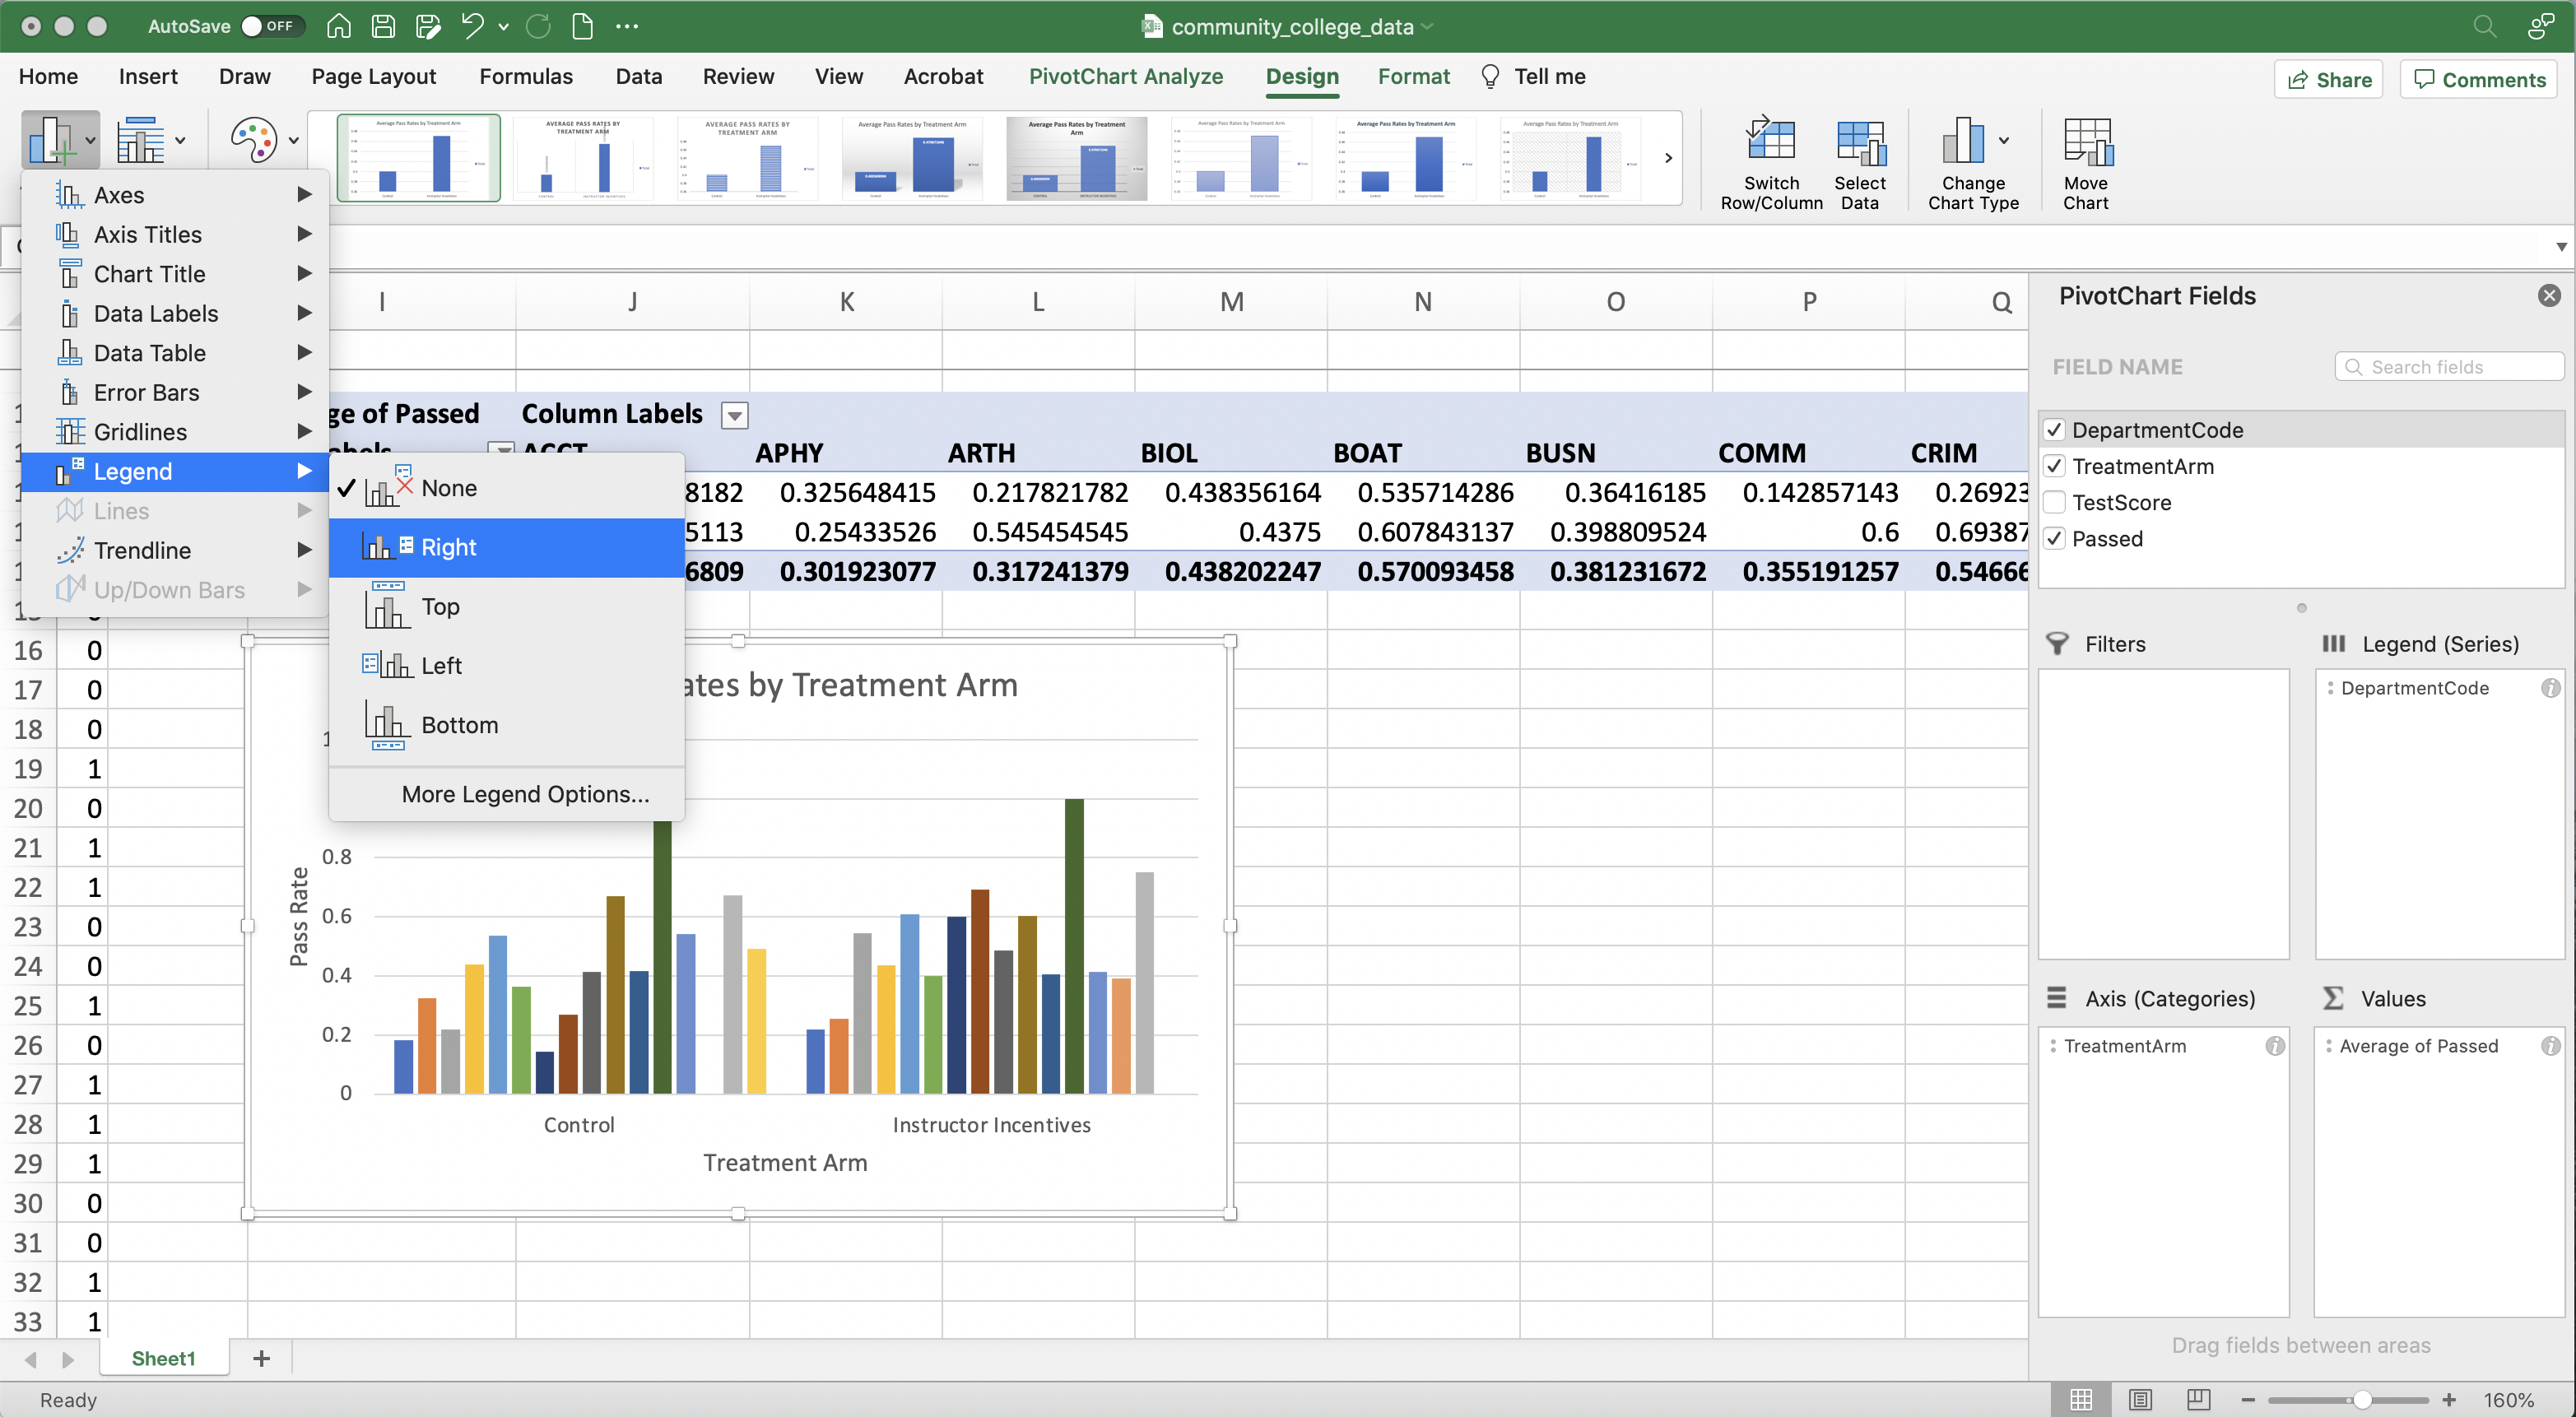
\includegraphics[width=1\linewidth]{images/01_adv_pivot3} 

}

\caption{Average Pass Rates by Treatment Arm and Department}\label{fig:advpivot3}
\end{figure}

Figure \ref{fig:advpivot3} displays the resulting figure. This is the resulting figure.

\begin{figure}

{\centering 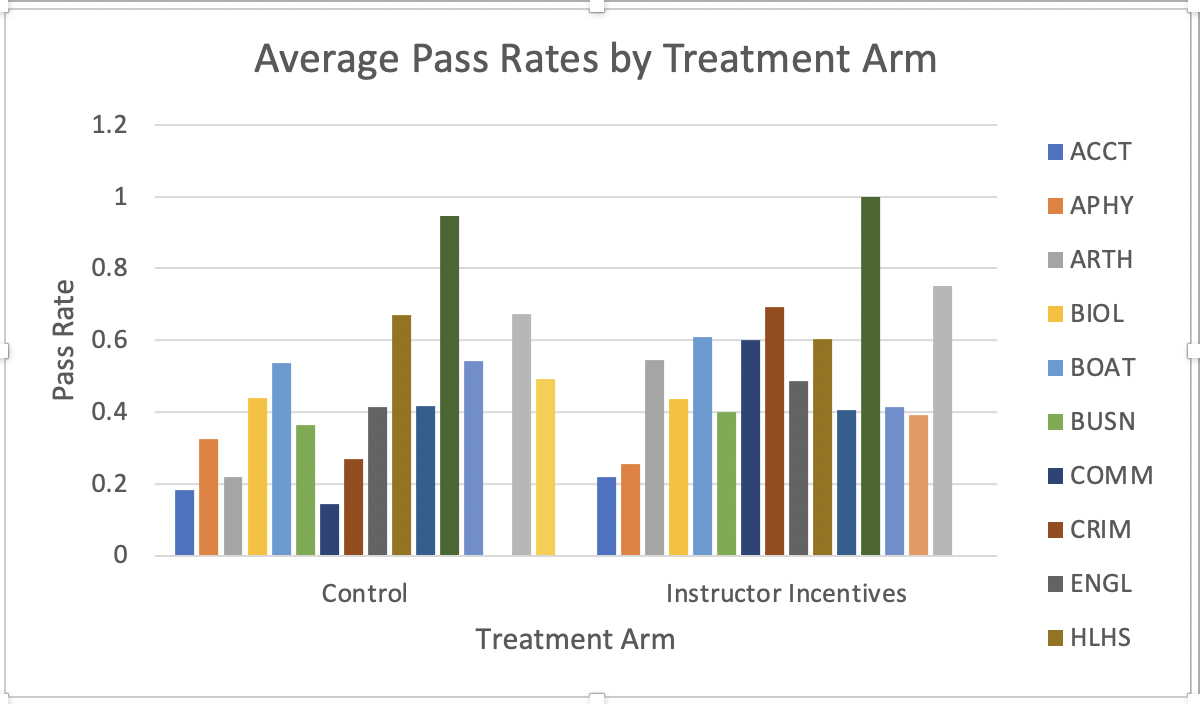
\includegraphics[width=1\linewidth]{images/01_adv_pivot4} 

}

\caption{Average Pass Rates by Treatment Arm and Department}\label{fig:advpivot4}
\end{figure}

This has all the elements of a good figure, but is it possible to improve it in any way? Let's think about our goal for this analysis. What do we want a reader to take away from this figure? Ideally, the reader should be able to look at different departments and see how the treatment effect varies by department. This is possible, but it takes a bit of work. For example, The ``Control'' bar for the ACCT department is pretty far away from the ``Instructor Incentives'' bar for the ACCT department. It would be much easier to quickly understand the treatment effect if the two bars were adjacent.

To make the bars adjacent, we can switch ``DepartmentCode'' to the horizontal Axis, and put ``TreatmentArm'' in the Legend(Series). In other words, the Pivot Chart fields should look like the fields below

\begin{figure}

{\centering 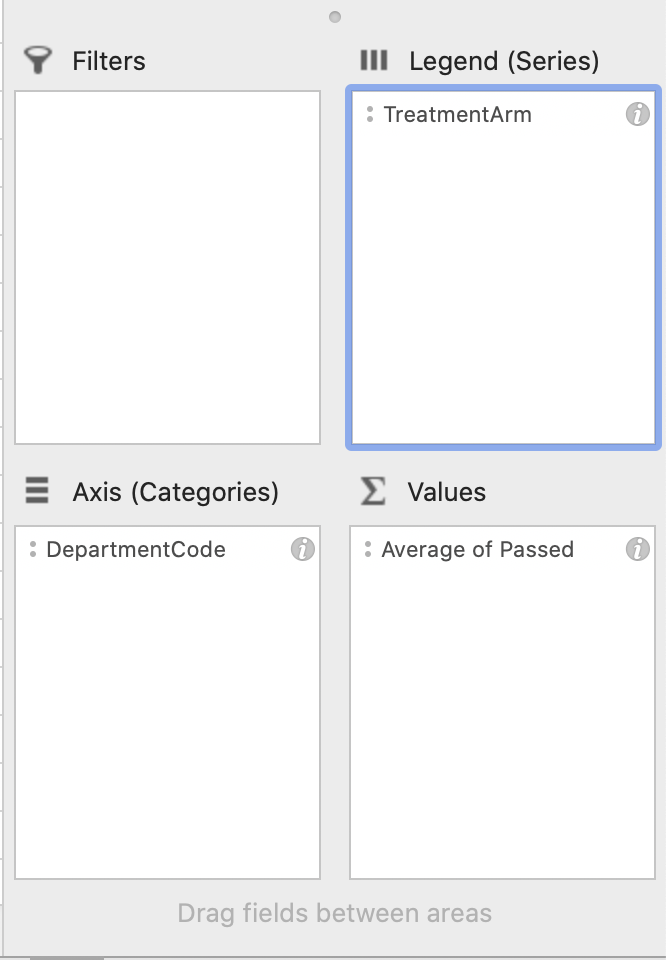
\includegraphics[width=0.4\linewidth]{images/01_adv_pivot5} 

}

\caption{Pivot Chart Fields}\label{fig:advpivot5}
\end{figure}

To complete the figure we just need to give it a more descriptive title and correct the horizontal axis label, which is no longer Treatment Arm. Figure \ref{fig:advpivot7} displays our final product.

\begin{figure}

{\centering 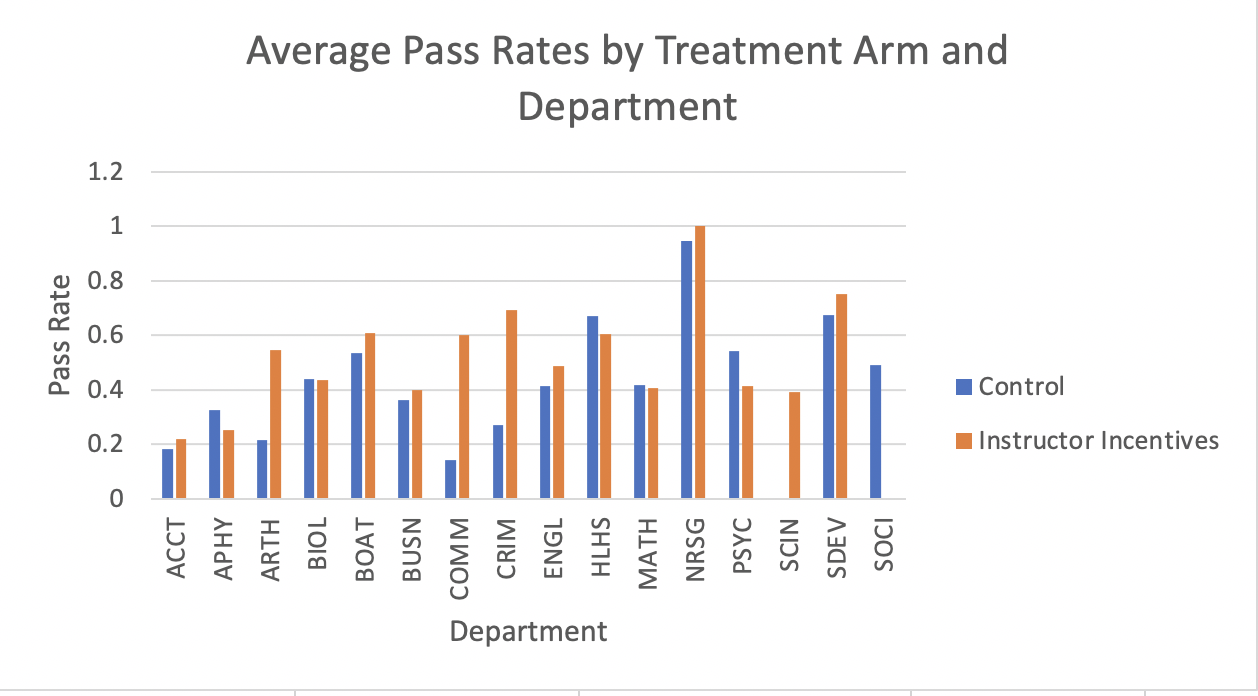
\includegraphics[width=1\linewidth]{images/01_adv_pivot7} 

}

\caption{Average Pass Rates by Treatment Arm and Department}\label{fig:advpivot7}
\end{figure}

Now it is easy for a reader to discern the treatment effect for every department. The general lesson here is to think hard about how your information displayed. Just because all of the information is there, doesn't mean it is necessarily easily digestible.

\section{Conclusion}\label{S:Conclusion}

In this module, we studied whether instructor incentives are effective in improving student performance. Using experimental data from Brownback and Sadoff (2020), we found that instructors who receive financial bonuses for each student who passes a course lead to significant increases in passing rates. However, the effects varied dramatically by department, with some departments showing enormous effects and others negligible effects. This is only part of the analysis in Brownback and Sadoff (2020). In this concluding section, let's talk about a few other results from their work.

So far, we have found performance increases in the course that is incentivized by financial incentives. But is there a cost to this increase in performance? For example, maybe instructors respond to the incentives by increasing the workload in their course. This may improve students' performance in the course, but it may come at the cost of neglecting other courses. Therefore, it could be that the treatment does not actually increase performance overall, but simply forces students to spend more time in one class relative to another.

However, Brownback and Sadoff (2020) collect grades for all courses a student is enrolled in, not just the courses in the experiment. In contrast to the hypothesis above, the authors find student outcomes in the treatment improve \textbf{in all courses}. This suggests positive spillovers of the treatment. Improved performance in one course leads to improved performance in others. If students feel overwhelmed by poor grades in one course they may ``give up'' on the rest of their courses. Therefore, a treatment that increases performance in a single course has the scope to increase performance in all courses.

This analysis shows evidence of positive effects, but only in the short term. Our real goal is to improve graduate rates. Again, the richness of the data in Brownback and Sadoff (2020) will come in handy here. The authors find that students in the treatment are about 2.8 percentage points more likely to transfer to a 4-year university than control students. This represents a 28 percent increase in the probability of transferring. Overall, this suggests financial incentives to instructors may be a particularly cost-effective way for community colleges to achieve a number of important goals.

We have focused on financial incentives for instructors, but maybe providing bonuses for students is even more effective. During the experiment, the authors offered free tuition for one summer course (face value of \$400) if they passed the test. Interestingly, the authors find this intervention had no impact on student performance.

To conclude, this paper asks an important question: how can we improve student performance in community colleges? In particular, are financial incentives for instructors effective? Before this paper, we had no clear answer to this question. Prior work focused on other settings and found differing results. By running a carefully designed experiment, the authors can convincingly answer this question. Financial incentives cannot only increase short-run performance but also increase long-term outcomes, such as overall course completion and transfer rates to 4-year universities.

\part{Stata}\label{part-stata}

\chapter{Intergenerational Mobility}\label{intergenerational-mobility}

\section{Opportunity Insights}\label{opportunity-insights}

In this section, we will be discussing the relationship between \textbf{intergenerational mobility} and the higher education system in the United States. Before we start exploring this relationship, we first need to understand the concept of intergenerational mobility. This concept asks a simple question: if you are born from low-income parents, what is the chance you move up the income distribution?

Generally, we think of societies with high rates of intergenerational mobility as more equal. If a society has high rates of intergenerational mobility, then that means individuals from low-income backgrounds have opportunities to move up the income distribution. One common path to upward mobility is the higher education system.

However, there are a few reasons why the higher education system may or may not lead to higher rates of intergenerational mobility. First, some colleges may not be particularly effective in increasing incomes. For example, for-profit colleges are often criticized as costly and low quality (see \href{https://www.nytimes.com/2020/06/17/business/coronavirus-for-profit-colleges.html}{NYT Article}). If a college accepts a large fraction of students from low-income backgrounds, it may still not promote intergenerational mobility if its students don't actually benefit from attending. Second, individuals from lower-income backgrounds may have lower access to the higher education system. The rising cost of college may be making this worse over time.

So how do we go about studying this question? We are going to use a dataset made publicly available by the researchers at \textbf{Opportunity Insights}. This data has made a big splash, both in academia and in policy circles. Figure \ref{fig:oi} shows a headline from an Upshot article about the dataset. In this article, the authors discuss how this dataset has led us to new insights about how access varies dramatically at some schools. The headline reads, ``Some Colleges Have More Students From the Top 1 Percent Than the Bottom 60. Find Yours''. If a school has more students from the top 1 percent than the bottom 60, then it probably does not promote intergenerational mobility. Most of the students are already from relatively well-off backgrounds. This is our first hint that colleges may vary dramatically in the extent they promote intergenerational mobility.

\begin{figure}

{\centering 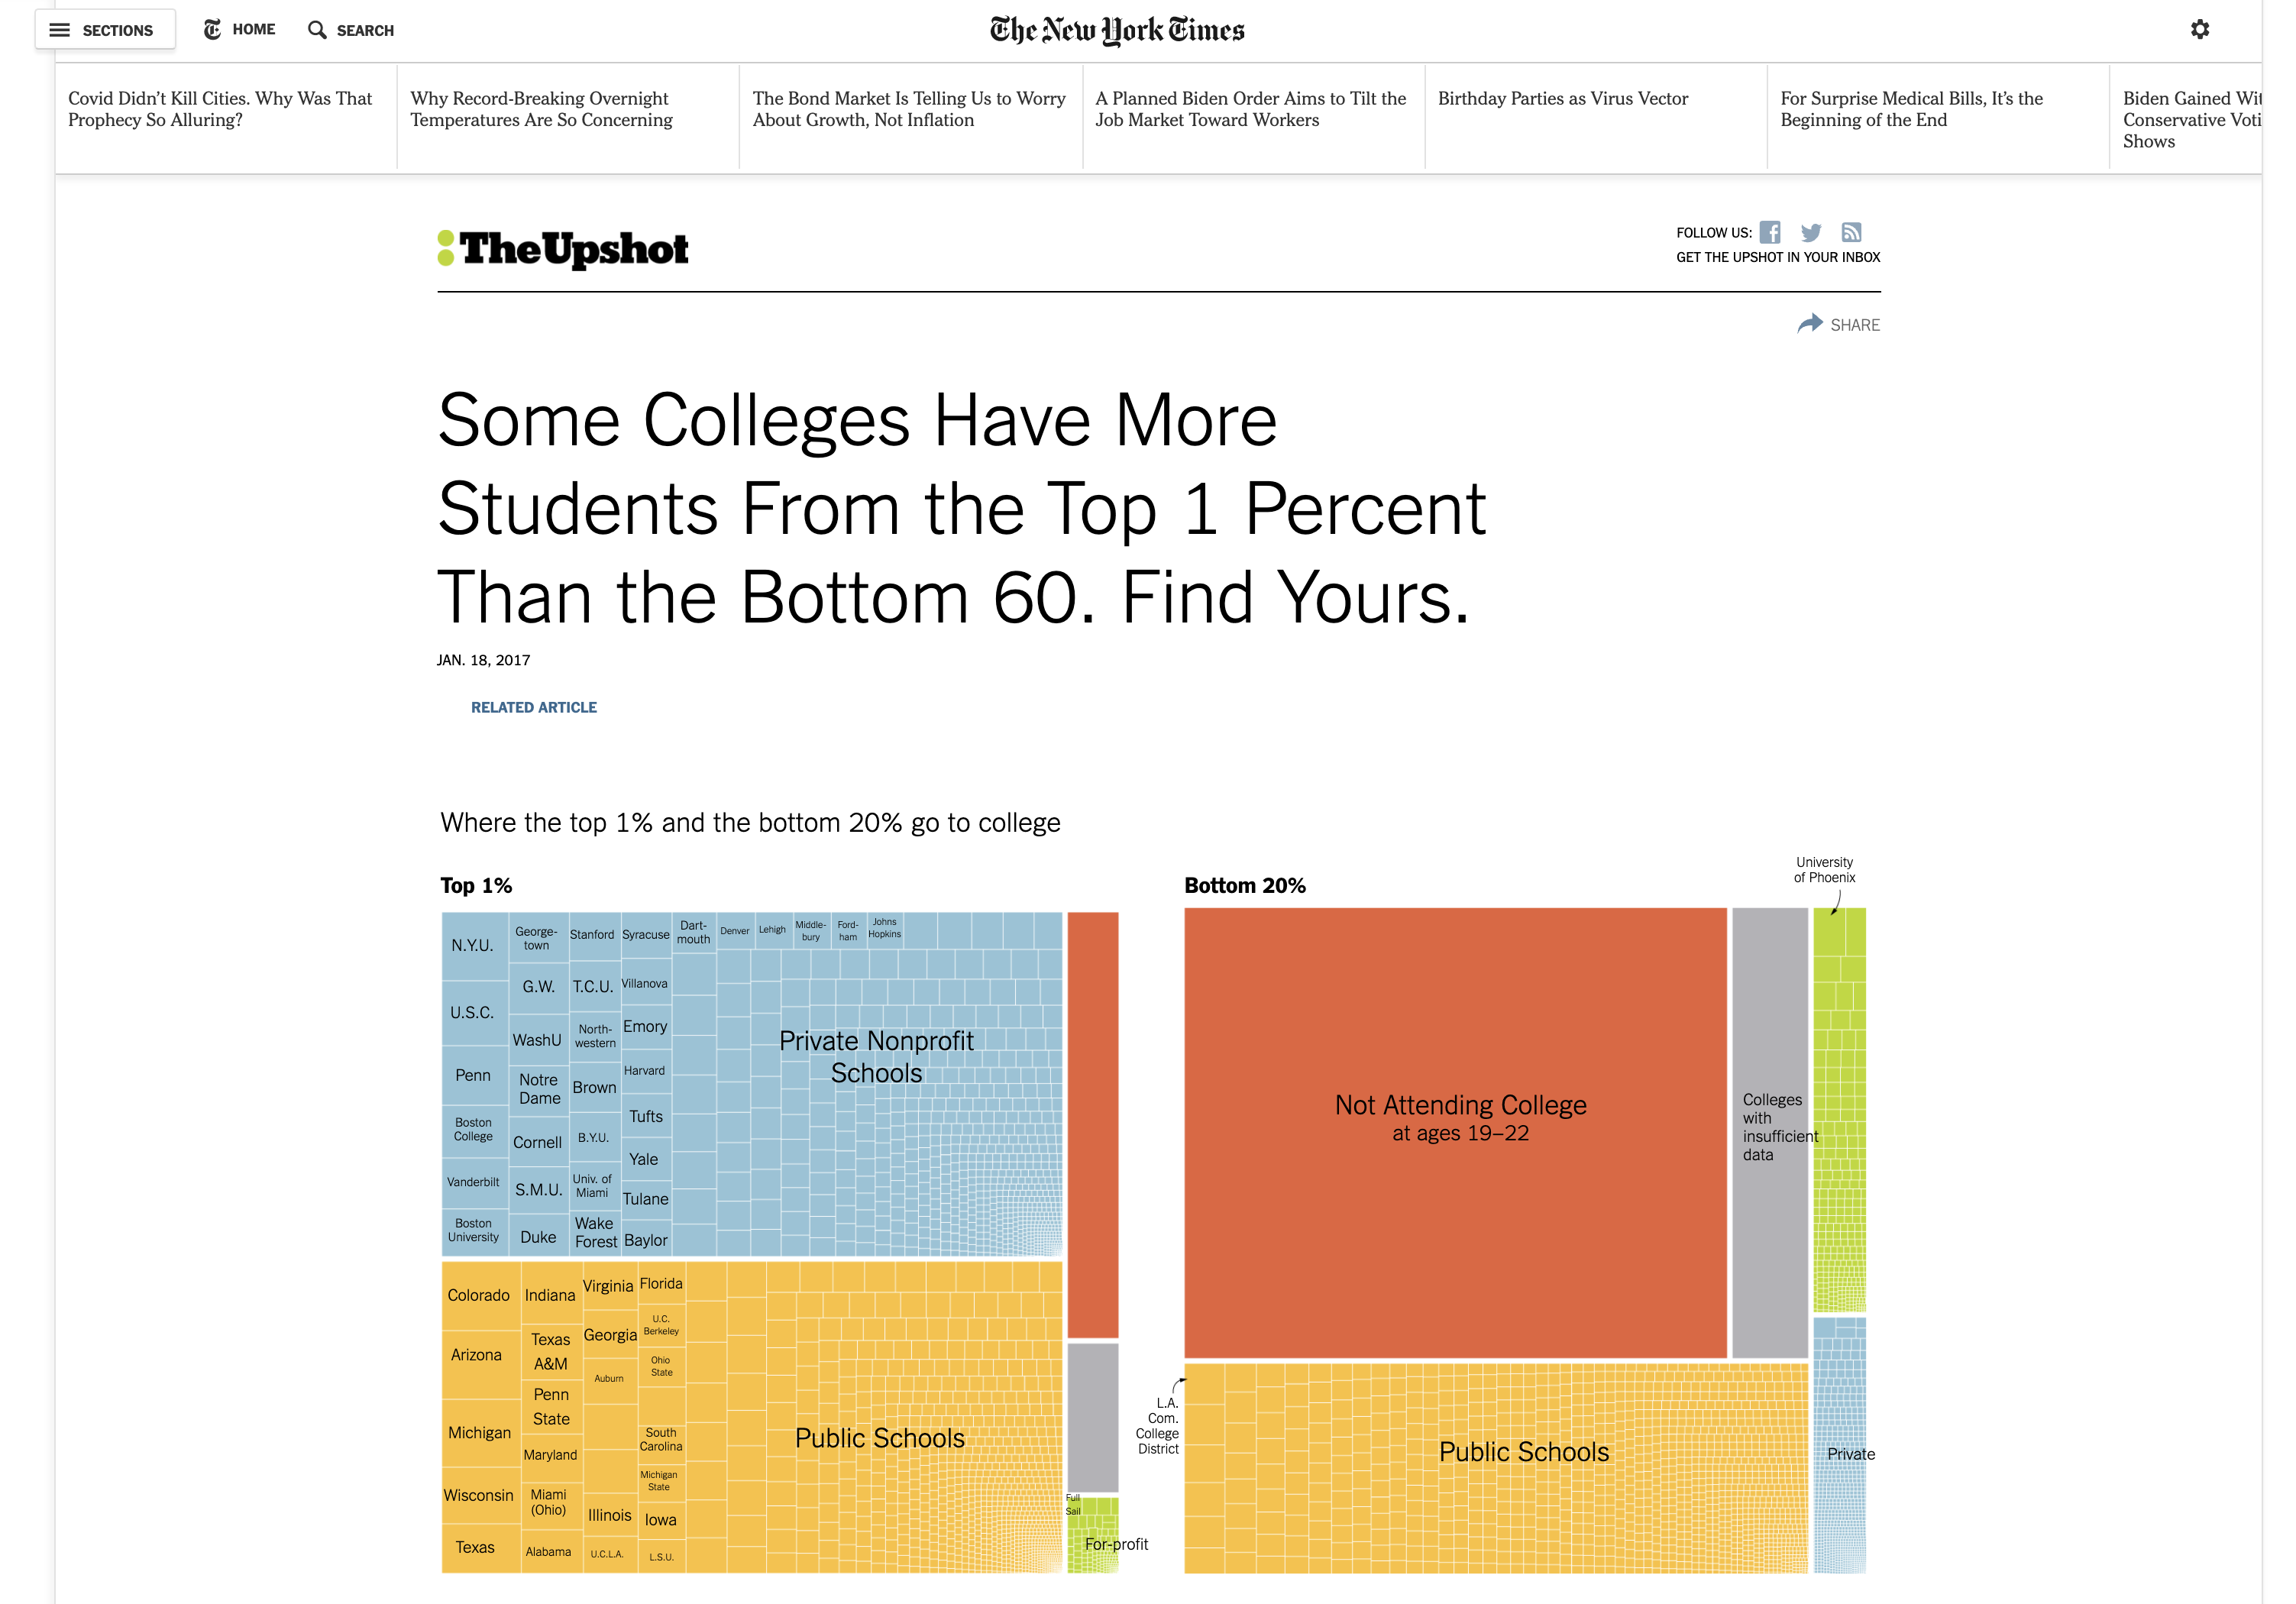
\includegraphics[width=1\linewidth]{images/02_oi} 

}

\caption{New York Times Graphic on Opportunity Insights}\label{fig:oi}
\end{figure}

Let's get a little bit more into the details on what data we will be using in this empirical application. The original data comes from federal income tax returns that have been linked to the tax records of universities and data from Pell Grants. The result is a dataset with (1) children linked to their parents (children are reported as dependents) (2) income data for both children and parents and (3) children linked to the universities they attended.

This will give us everything we need to know to understand how a given college promotes intergenerational mobility. It will allow us to know both the background of students attending a given college as well as their eventual earnings. It is important to emphasize that this was a huge data task that gives us a new way to study an important question.

We have discussed at a high level the concept of intergenerational mobility. But when we turn to the data, we will need to compute a metric of intergenerational mobility that allows us to compare across colleges. Before introducing this measure, we will introduce a statistical concept that will be important throughout the course, and in particular, in understanding our measure of intergenerational mobility: \textbf{quantiles}.

\section{Quantiles}\label{quantiles}

To begin our discussion of quantiles, let's imagine we have a small dataset of only 10 individuals. Each individual reports an income (in the thousands) and we sort the ten individuals based on their income.

\[          
\{5,6,20,29,38,42,55,62,80,88\} \nonumber
\]

We can break up the data into equal-sized groups based on income. Each equal-sized group is a \textbf{quantile}. For example, imagine we break the 10 individuals into 5 groups (or 5 quantiles).

\[
            \{\underbrace{5,6}_{Q1},\underbrace{20,29}_{Q2},\underbrace{38,42}_{Q3},\underbrace{55,62}_{Q4},\underbrace{80,88}_{Q5}\} \nonumber
\]

When we break up the observations into 5 equal-sized groups, this is referred to as breaking the data into \textbf{quintiles}. Q1 is referred to as the first quintile (or lowest quintile). Q5 is referred to as the fifth quintile (or highest quintile). Quintiles will be important for us because we will use them to define intergenerational mobility. In particular, we have conceptualized intergenerational mobility as the movement from a low-income background to high income. But low income and high income do not have any exact definition. The researchers at Opportunity Insights use quintiles to define these terms.

In particular, an individual is defined as coming from low-income parents if the individual's parents are in the bottom quintile (Q1) of the income distribution. The bottom quintile implies the parents are in the bottom 20 percent of the income distribution. An individual is defined as a high-income individual if this individual is in the top quintile (Q5) of the income distribution, or equivalently, the top 20 percent of the income distribution.

Quintiles are just one way to break up the data. If we break the data into four equal-sized groups, then we have broken the data into quartiles. If we break the data into a hundred equal-sized groups, we have broken the data into percentiles. In general, if we break the data into \(q\) groups, we have created \(q\) quantiles.

Certain percentiles are often reported as descriptive statistics. For example, the median (50\(^{th}\) percentile) is often reported as a summary statistic. In 2019, according to the U.S. Census, the median household income was \$68,703. This implies that 50 percent of households had income less than \$68,703, while 50 percent had income more than \$68,703.

\textbf{Question: If an individual is at the 33rd percentile of earnings, then this individual has\ldots{}}

\begin{itemize}
\tightlist
\item
  \begin{enumerate}
  \def\labelenumi{(\Alph{enumi})}
  \tightlist
  \item
    Lower earnings than 33 percent of individuals\\
  \end{enumerate}
\item
  \begin{enumerate}
  \def\labelenumi{(\Alph{enumi})}
  \setcounter{enumi}{1}
  \tightlist
  \item
    Lower earnings than 67 percent of individuals\\
  \end{enumerate}
\item
  \begin{enumerate}
  \def\labelenumi{(\Alph{enumi})}
  \setcounter{enumi}{2}
  \tightlist
  \item
    Higher earnings than 67 Percent of individuals
  \end{enumerate}
\end{itemize}

\section{Mobility Definition}\label{mobility-definition}

Now that we understand quantiles, we will define a college's intergenerational mobility rate. Intuitively, a college will promote intergenerational mobility if it (1) admits students from low-income backgrounds and (2) these students become high earners later in life. Again, we have defined low income as the bottom quintile of earnings, while high income is the top quintile of earnings. We will define the \textbf{mobility rate} as the fraction of low-income students, multiplied by the probability these low-income students go on to become high earners:

\[
\text{mobility rate}= \underbrace{\text{(frac. of students from Q1)}}_{\text{Acess}} \; \cdot \; \underbrace{\text{(frac. of Q1 that reach Q5)}}_{\text{Success}} \nonumber
\]

Let's talk about each of these terms independently. ``Access'' depends on the fraction of students enrolled in a school that come from low-income backgrounds, or Q1. There is potential for schools with high access to have large impacts on intergenerational mobility. But this might not necessarily be true. For example, some work has found while for-profit colleges tend to admit disadvantaged individuals, the outcomes for these individuals tend to be poor (see Deming, Goldin and Katz 2013).\citep{deming2013profit} Therefore, even though the Access rate might be high, these schools will not tend to promote intergenerational mobility. The reason is due to the second term: Success. This measures the fraction of students from low-income backgrounds that reach the top quintile of earnings.

Intuitively, we can interpret the mobility rate as the fraction of students that are from low-income backgrounds that reach high income at a school. For example, if 10 percent of a school's enrollment comes from a low-income background, and half of these students end up in the top quintile of earnings, then that means 5 percent (overall) of the student body came from low-income backgrounds and achieved high income. This number is equal to the school's mobility rate.

But now let's get into the specifics of the data. How do we (exactly) determine if a student comes from a low-income background? Here are the steps:

\begin{itemize}
\tightlist
\item
  \begin{enumerate}
  \def\labelenumi{\arabic{enumi}.}
  \tightlist
  \item
    Take all parents that have a child in the same year (e.g.~1985)
  \end{enumerate}
\item
  \begin{enumerate}
  \def\labelenumi{\arabic{enumi}.}
  \setcounter{enumi}{1}
  \tightlist
  \item
    Compute the average income for these parents when children are 15-19 (i.e.~from 2000-2004)
  \end{enumerate}
\item
  \begin{enumerate}
  \def\labelenumi{\arabic{enumi}.}
  \setcounter{enumi}{2}
  \tightlist
  \item
    If parents' income is in the bottom 20 percent over this period (i.e.~in Q1), then classify students as coming from a low-income background
  \end{enumerate}
\end{itemize}

Now that we have a definition for low-income background, how (exactly) do we determine if a student becomes a high earner?

\begin{itemize}
\tightlist
\item
  \begin{enumerate}
  \def\labelenumi{\arabic{enumi}.}
  \tightlist
  \item
    Take all individuals that are the same age and calculate earnings in 2014
  \end{enumerate}
\item
  \begin{enumerate}
  \def\labelenumi{\arabic{enumi}.}
  \setcounter{enumi}{1}
  \tightlist
  \item
    If an individual's income is in the top 20 percent relative to individuals the same age (i.e.~in Q5), then classify the student as a high earner
  \end{enumerate}
\end{itemize}

A general lesson here is to understand the details before you proceed with the analysis. In this example, low income and high income have very specific definitions. We need to understand our variables and how they are measured before we can dive into our analysis.

\textbf{Question: Imagine 10 percent of College A's students come from low-income backgrounds, and 20 percent of these individuals go on to become high earners. In contrast, 5 percent of College B's students come from low-income backgrounds and 50 percent of these individuals go on to become high earners. Which college has the higher mobility rate?}

\begin{itemize}
\tightlist
\item
  \begin{enumerate}
  \def\labelenumi{(\Alph{enumi})}
  \tightlist
  \item
    College A\\
  \end{enumerate}
\item
  \begin{enumerate}
  \def\labelenumi{(\Alph{enumi})}
  \setcounter{enumi}{1}
  \tightlist
  \item
    College B\\
  \end{enumerate}
\item
  \begin{enumerate}
  \def\labelenumi{(\Alph{enumi})}
  \setcounter{enumi}{2}
  \tightlist
  \item
    They have the same\\
  \end{enumerate}
\item
  \begin{enumerate}
  \def\labelenumi{(\Alph{enumi})}
  \setcounter{enumi}{3}
  \tightlist
  \item
    Not possible to tell
  \end{enumerate}
\end{itemize}

\section{Stata GUI}\label{stata-gui}

Before digging into the Opportunity Insights dataset, we first need to learn how to use Stata. Every time you launch Stata, you will be greeted by the Graphical User Interface (GUI) you see in Figure \ref{fig:gui}

\begin{figure}

{\centering 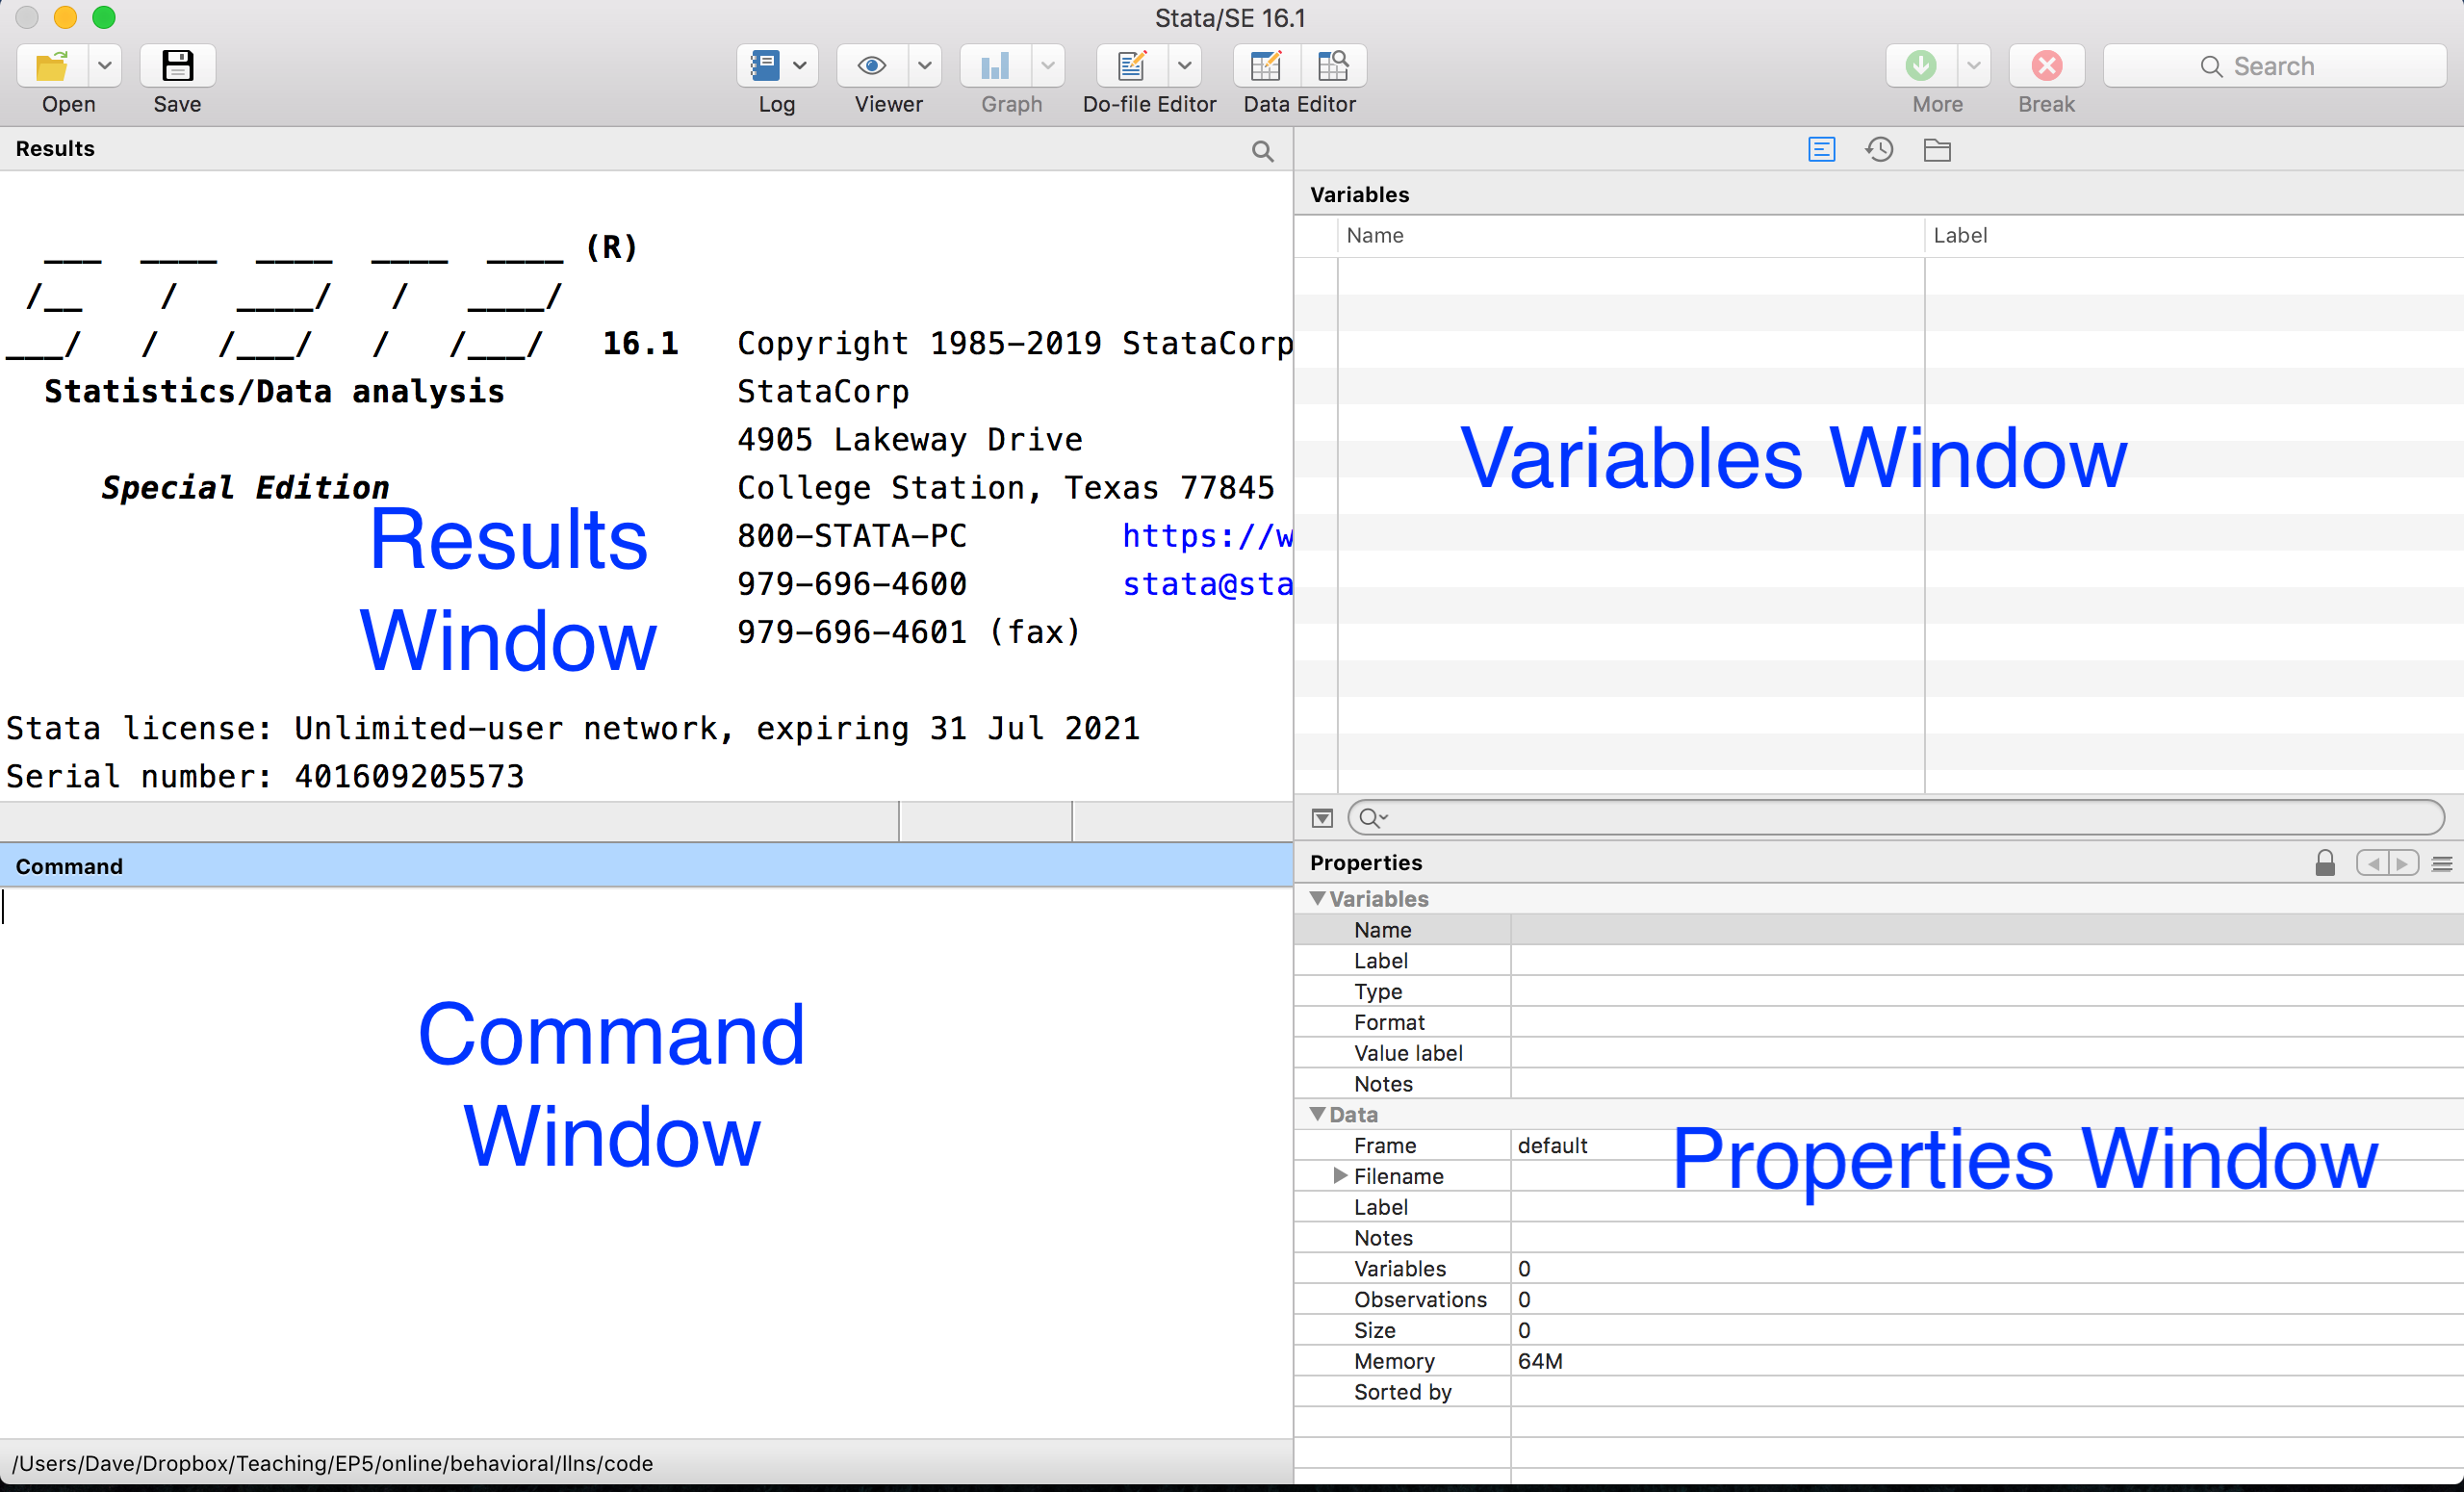
\includegraphics[width=1\linewidth]{images/02_main} 

}

\caption{Stata Graphical User Interface}\label{fig:gui}
\end{figure}

There are 4 main panels here. Let's start in the bottom left: the Command window. This is where you can type code. When you press enter, the code will executed. When we learn how to use Stata as a calculator, this is where we will type the code.

When we execute code, any resulting output will be displayed in the Results window. When we learn how to use Stata as a calculator, this is where the results will be displayed.

When we load data, the names of the variables in the dataset will appear in the first column. Many times, datasets come with labels that give us more description about the variable. For example, in the figure below there is one variable named \texttt{income} with the label \texttt{Total\ Annual\ Income}.

\begin{figure}

{\centering 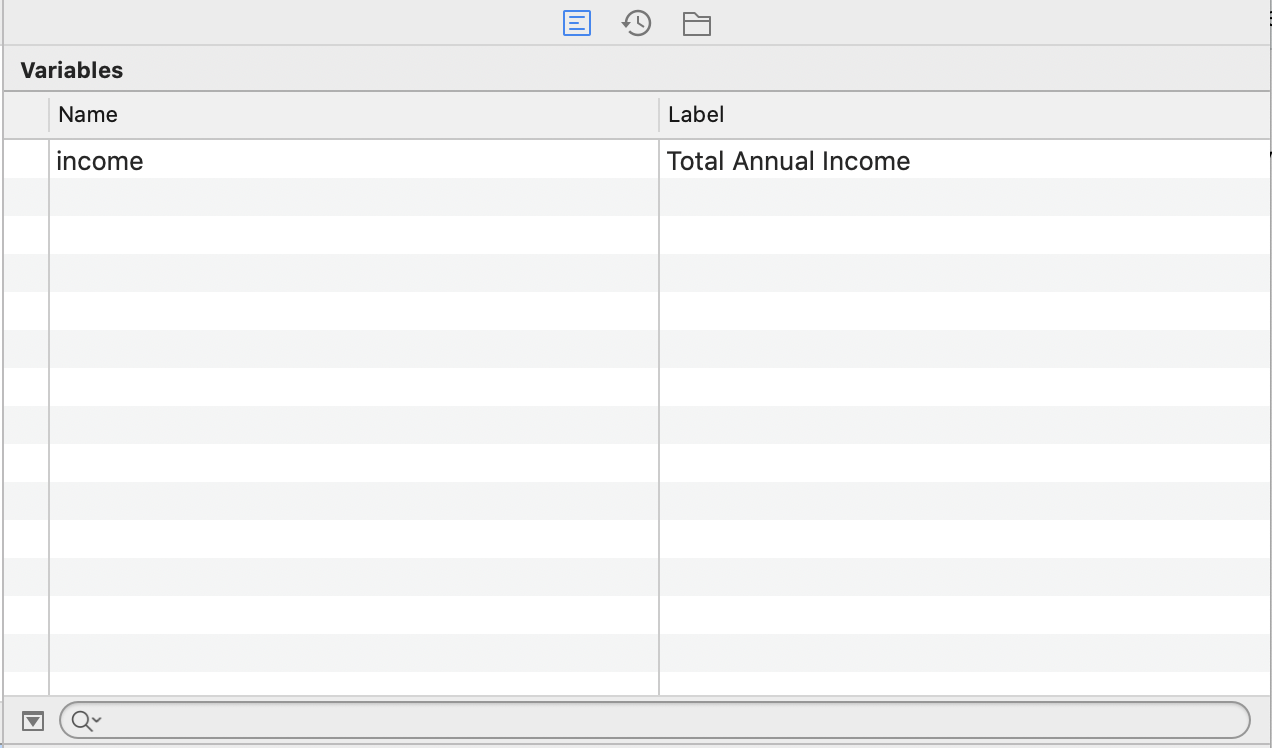
\includegraphics[width=0.75\linewidth]{images/02_example_income} 

}

\caption{Variables Window Example}\label{fig:main}
\end{figure}

The Properties window gives us more information about the variables and data loaded in memory. For example, in addition to the name and label of a variable, the type (i.e.~numeric or string) and format of the variable (i.e.~how the variable will be displayed). Additionally, there is information about the size of the data (number of variables, observations, etc.)

Now that we have learned about the various windows, we are going to execute our first line of code. In particular, we are going to use Stata as a calculator by typing \texttt{display} followed by a mathematical expression.

For example, to compute \texttt{2+2} type

\begin{Shaded}
\begin{Highlighting}[]
\KeywordTok{display}\NormalTok{ 2+2}
\NormalTok{file gapminder.dta }\KeywordTok{not}\NormalTok{ Stata }\KeywordTok{format}
\FunctionTok{r}\NormalTok{(610);}


\NormalTok{4}
\end{Highlighting}
\end{Shaded}

The result will be visible in the Results window. \texttt{display} is called a command in Stata. Stata comes with many commands that will be useful to explore and analyze our data. Whenever you learn a new command in Stata it is helpful to look at the help file that comes along with this command. To access the help file for the display command type \texttt{help\ display} into the command window. This will open up a file that has instructions on how to use the given command

The first thing you will generally see in any help file is the syntax of the command. Syntax refers to the format of the code. It is similar to the ``grammar'' of the software language. If you use incorrect grammar in language, you may not be expressing the right meaning. Similarly, if you use the wrong syntax in software language, you may not get the correct output, and more than likely, an error will be reported

Figure \ref{fig:helpdisplay} shows the Syntax from the help file for the display command.

\begin{figure}

{\centering 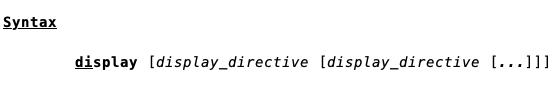
\includegraphics[width=1\linewidth]{images/02_display_help_file} 

}

\caption{Variables Window Example}\label{fig:helpdisplay}
\end{figure}

The fact that \texttt{di} is underlined means to use the display command you only need to type \texttt{di} as a shortcut. Many commands in Stata have shortcuts associated with them. To figure out those shortcuts, you just need to open the help file. We will fill in the \texttt{{[}display\_directive{]}} in a couple of ways

We can use Stata to perform calculations just like you would in a calculator. For example, for subtraction, type:

\begin{Shaded}
\begin{Highlighting}[]
\KeywordTok{di}\NormalTok{ 6{-}4}
\NormalTok{file gapminder.dta }\KeywordTok{not}\NormalTok{ Stata }\KeywordTok{format}
\FunctionTok{r}\NormalTok{(610);}


\NormalTok{2}
\end{Highlighting}
\end{Shaded}

For multiplication type:

\begin{Shaded}
\begin{Highlighting}[]
\KeywordTok{di}\NormalTok{ 2*4}
\NormalTok{file gapminder.dta }\KeywordTok{not}\NormalTok{ Stata }\KeywordTok{format}
\FunctionTok{r}\NormalTok{(610);}


\NormalTok{8}
\end{Highlighting}
\end{Shaded}

For division type:

\begin{Shaded}
\begin{Highlighting}[]
\KeywordTok{di}\NormalTok{ 12/2}
\NormalTok{file gapminder.dta }\KeywordTok{not}\NormalTok{ Stata }\KeywordTok{format}
\FunctionTok{r}\NormalTok{(610);}


\NormalTok{6}
\end{Highlighting}
\end{Shaded}

We can also use \texttt{display} to print text. This can be very helpful when writing programs. For example, if something goes wrong in a program, you, might want to display an error code. To display the words in Stata, you just need to put the words you would like to display in quotation marks. For example, to display ``Hello World'' type:

\begin{Shaded}
\begin{Highlighting}[]
\KeywordTok{display} \StringTok{"Hello World"}
\NormalTok{file gapminder.dta }\KeywordTok{not}\NormalTok{ Stata }\KeywordTok{format}
\FunctionTok{r}\NormalTok{(610);}


\NormalTok{Hello World}
\end{Highlighting}
\end{Shaded}

Words are referred to as strings in Stata (later we will have string variables and numeric variables). When you reference a string, need to put in quotation marks. For example, if we were to type \texttt{display\ Hello\ World} into Stata, we would get the error depicted in Figure \ref{fig:helloerror}.

\begin{figure}

{\centering 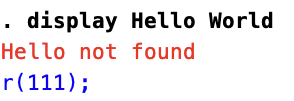
\includegraphics[width=0.5\linewidth]{images/02_hello_error} 

}

\caption{Forgetting Quotation Marks When Referencing Strings}\label{fig:helloerror}
\end{figure}

\texttt{Hello} was not found because Stata looked for a command or variable named \texttt{Hello}, but could not find one, and therefore reported an error. The command did not realize it was just meant to display text, because the text was not in quotation marks.

\section{Do-files}\label{do-files}

So far, we have discussed how to execute code by typing it into the command window. In practice, we will seldom use the command window to execute code. Instead, we will use a \textbf{do-file}.

To understand the importance of a do-file, let's imagine you have a project that has a large number of steps. Maybe you need to clean the data (usually a necessity) and then run a large number of results. A single project could end up being thousands of lines of code. What would it entail to complete this project if you were to use the command line?

You would need to type in the lines of code one at a time. But what if you make a mistake at the beginning of your project. For example, you accidently deleted some observations relevant to your analysis. This is a disaster! You now need to remember what you did, type all of the code again, and then execute it.

A better way to approach any project is to use a do-file. A do-file allows you to run multiple lines of code sequentially. You can save your progress periodically, just as you save your progress when writing a paper in a text editing program like Microsoft Word. Then, if you realize you made a mistake early in the project, you can just alter that one line of code and then re-run the entire project.

To begin, we need to learn how to open a do-file. At the top of the GUI there is an icon that looks like a piece of paper and pencil above it (see Figure \ref{fig:maincopy}).

\begin{figure}

{\centering 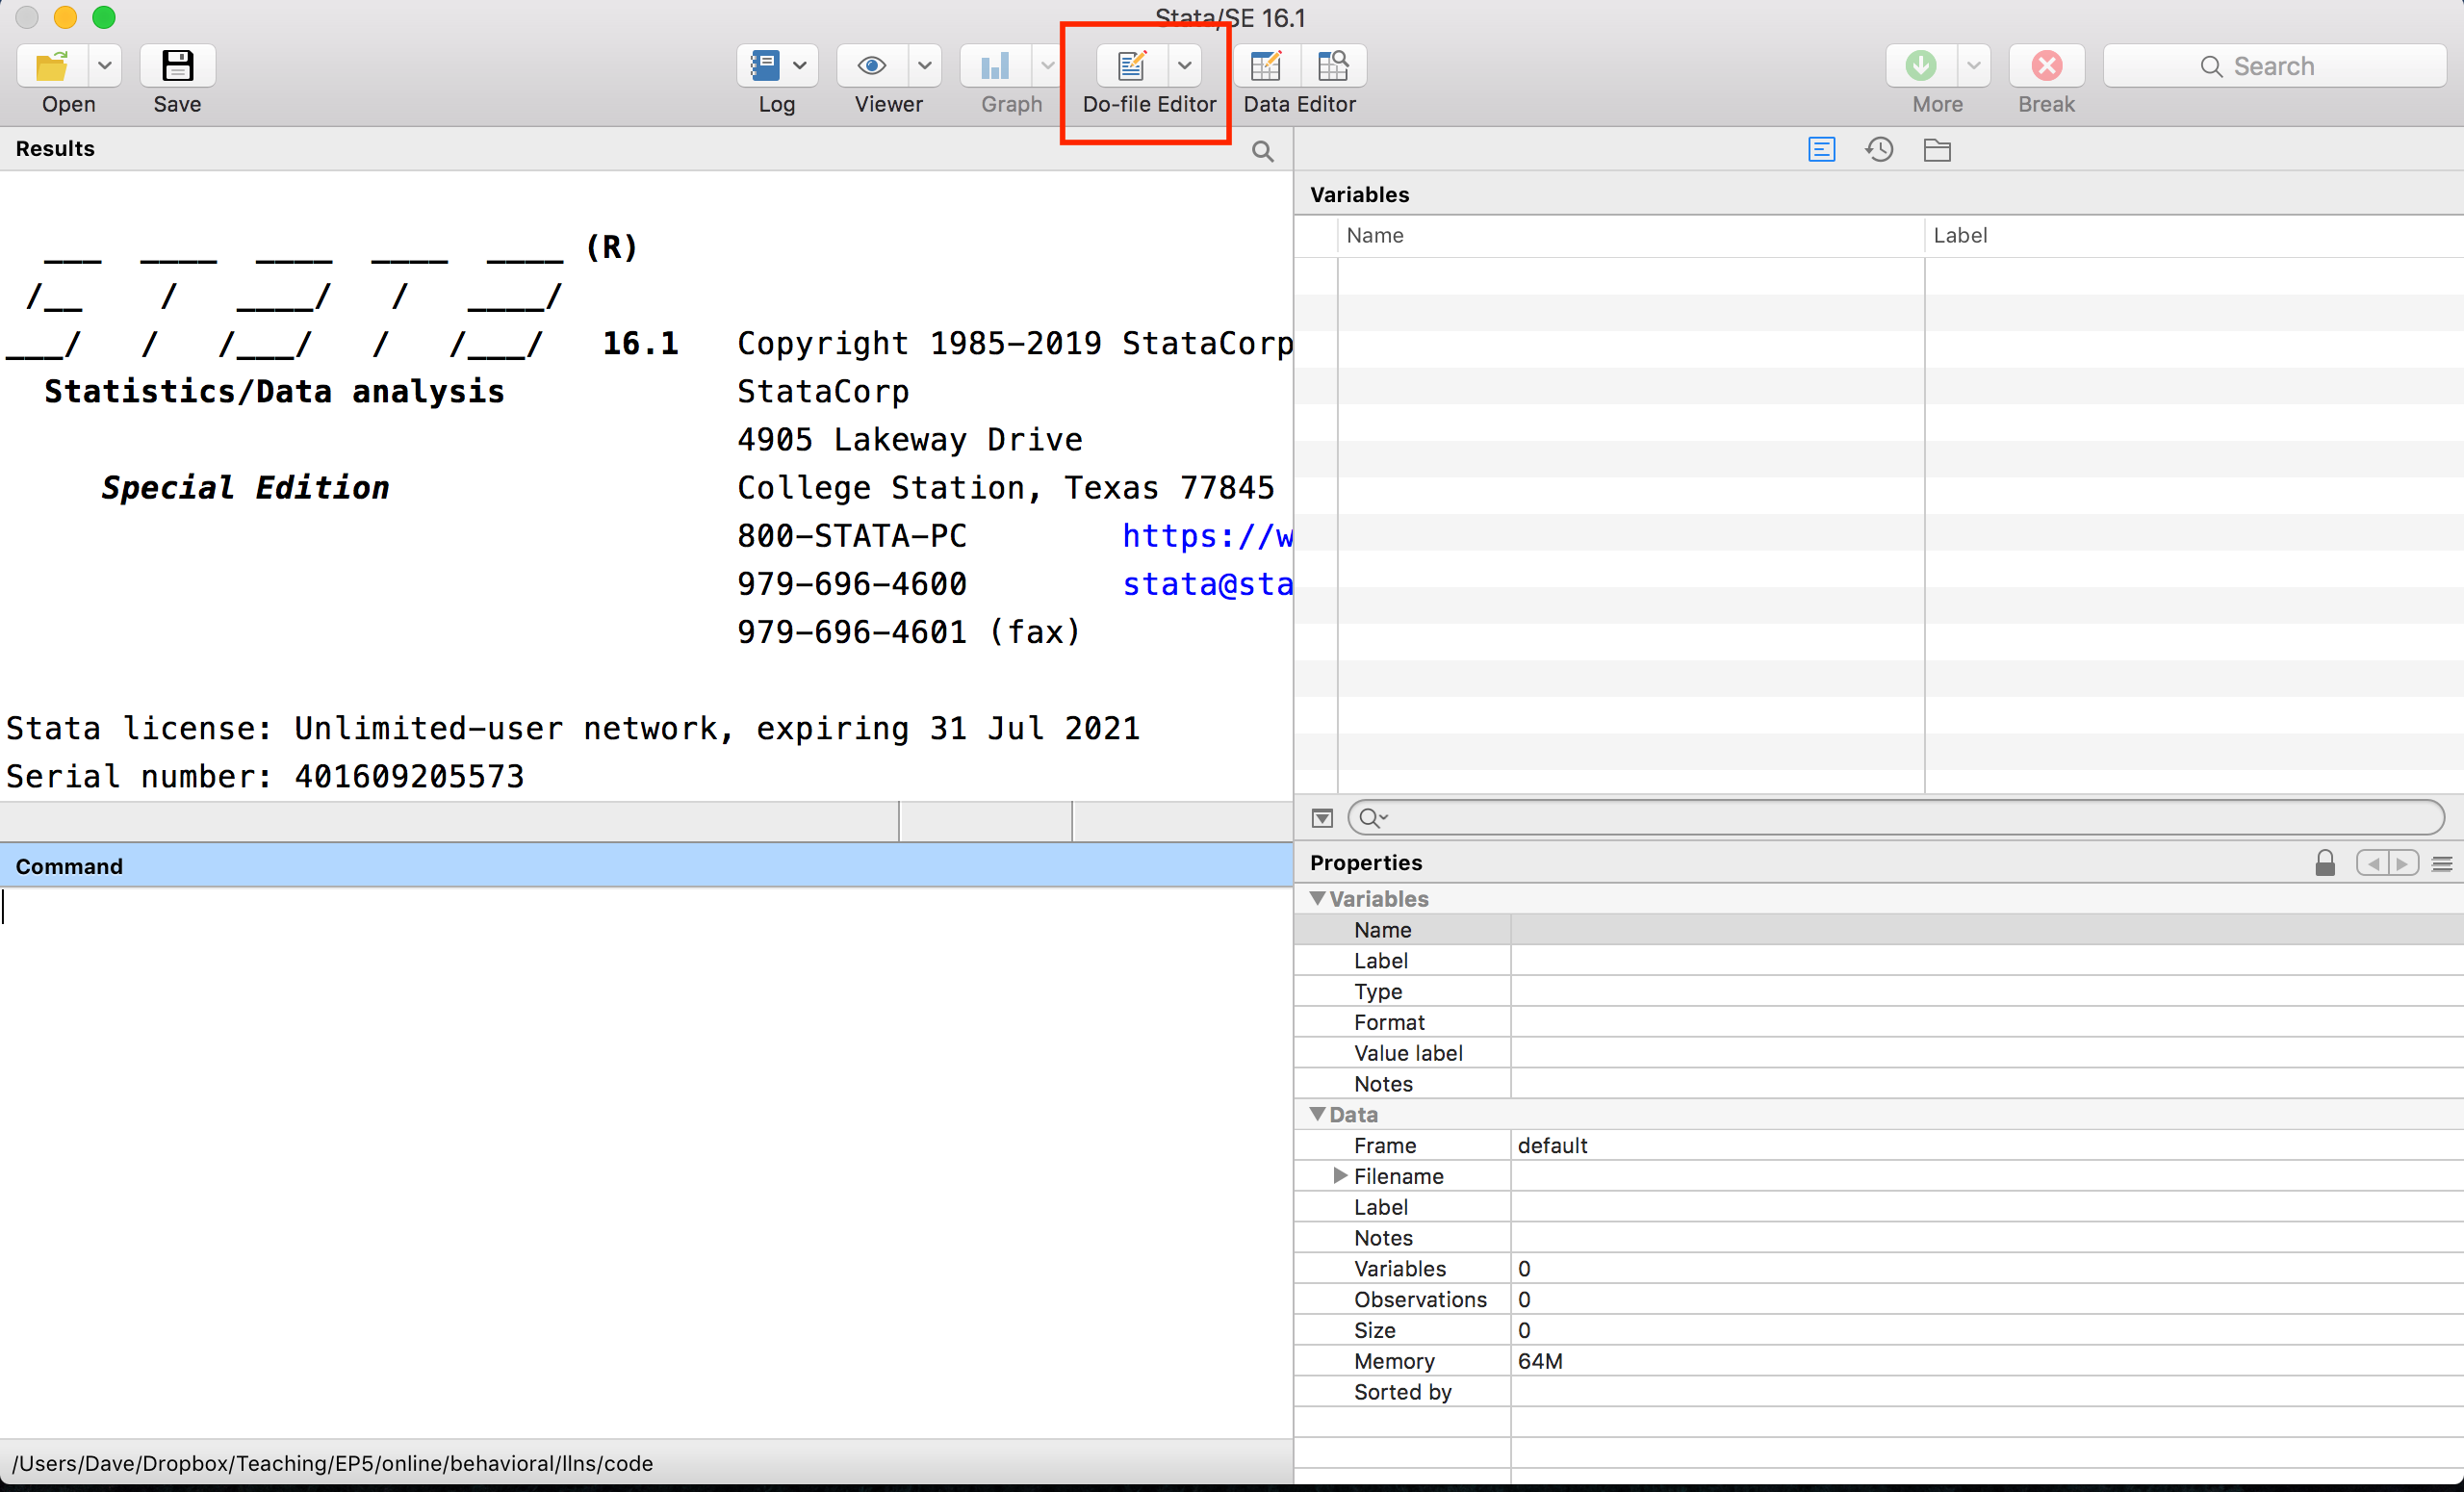
\includegraphics[width=0.75\linewidth]{images/02_main copy} 

}

\caption{Opening a New Do-File in Stata}\label{fig:maincopy}
\end{figure}

Figure \ref{fig:dofileicon} shows a larger version of the do-file icon.

\begin{figure}

{\centering 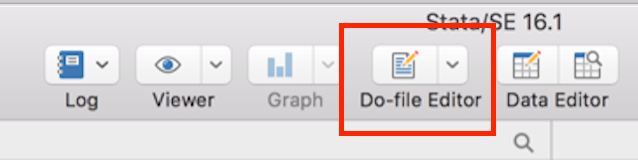
\includegraphics[width=0.75\linewidth]{images/02_icon} 

}

\caption{Do-File Icon}\label{fig:dofileicon}
\end{figure}

To open a new do-file we can simply click the icon. When you do, you will see a blank file. This is where we are going to type code into (see Figure \ref{fig:dofile1}).

\begin{figure}

{\centering 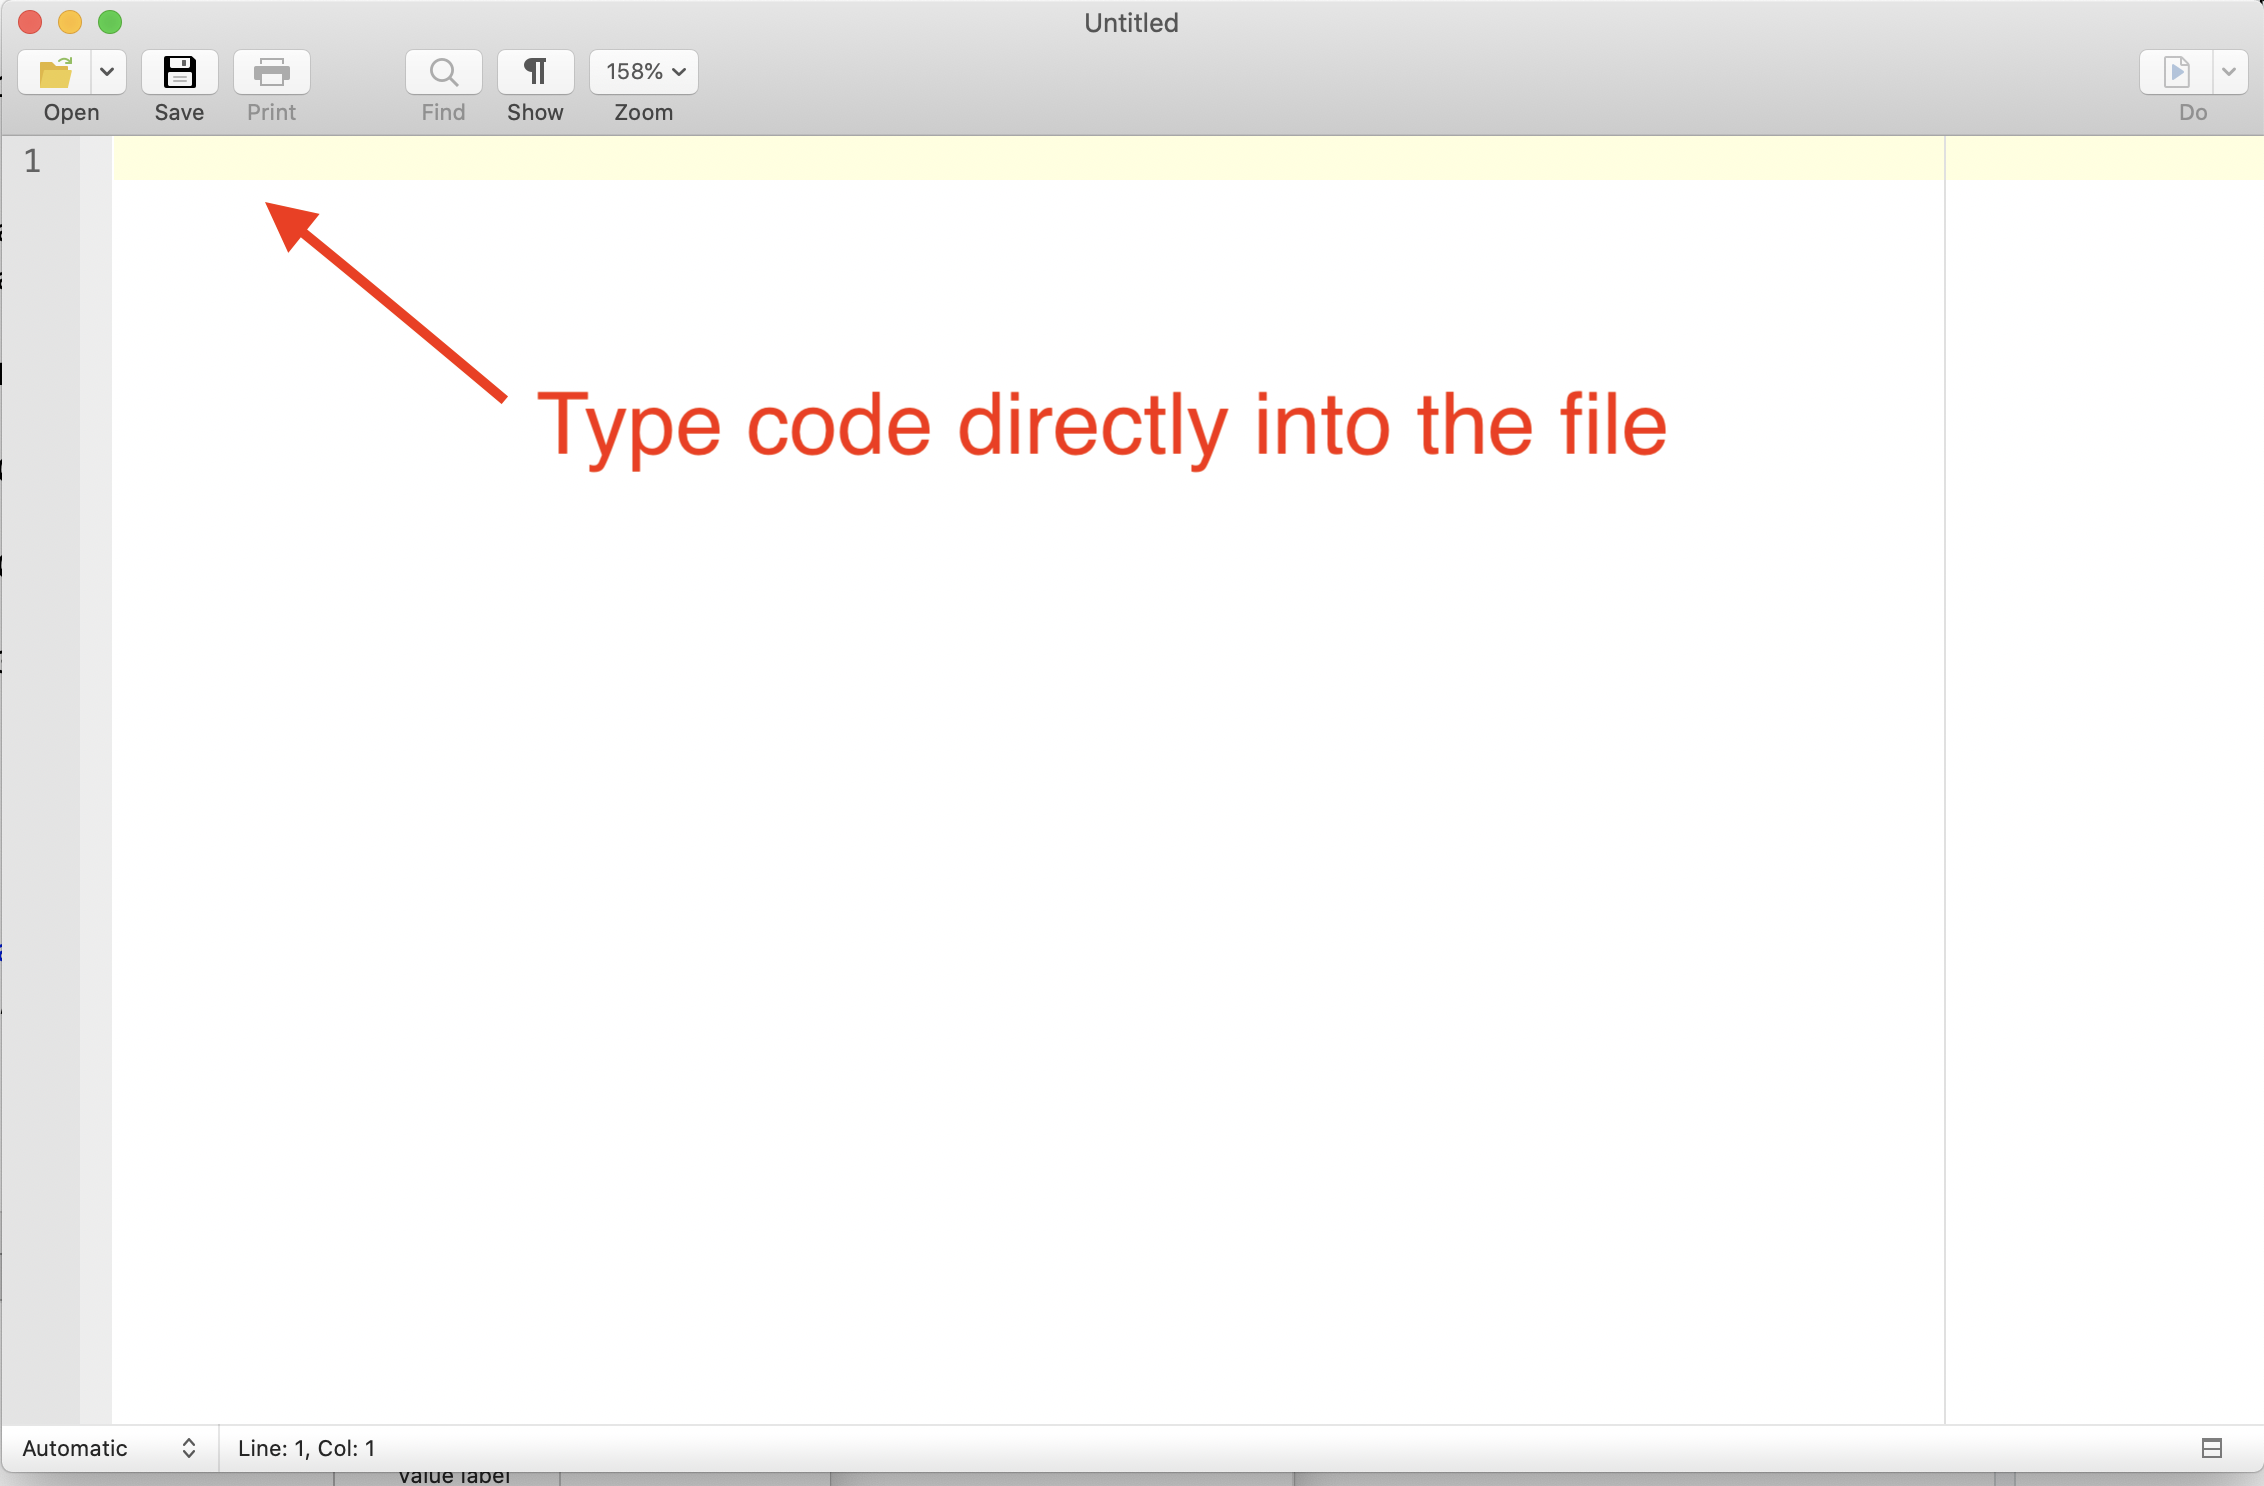
\includegraphics[width=0.75\linewidth]{images/02_dofile1} 

}

\caption{Blank Do-File}\label{fig:dofile1}
\end{figure}

For example, if we want Stata to compute the sum of 2+2, we would type \texttt{display\ 2+2} into the dofile, as seen in Figure \ref{fig:dofile2}.

\begin{figure}

{\centering 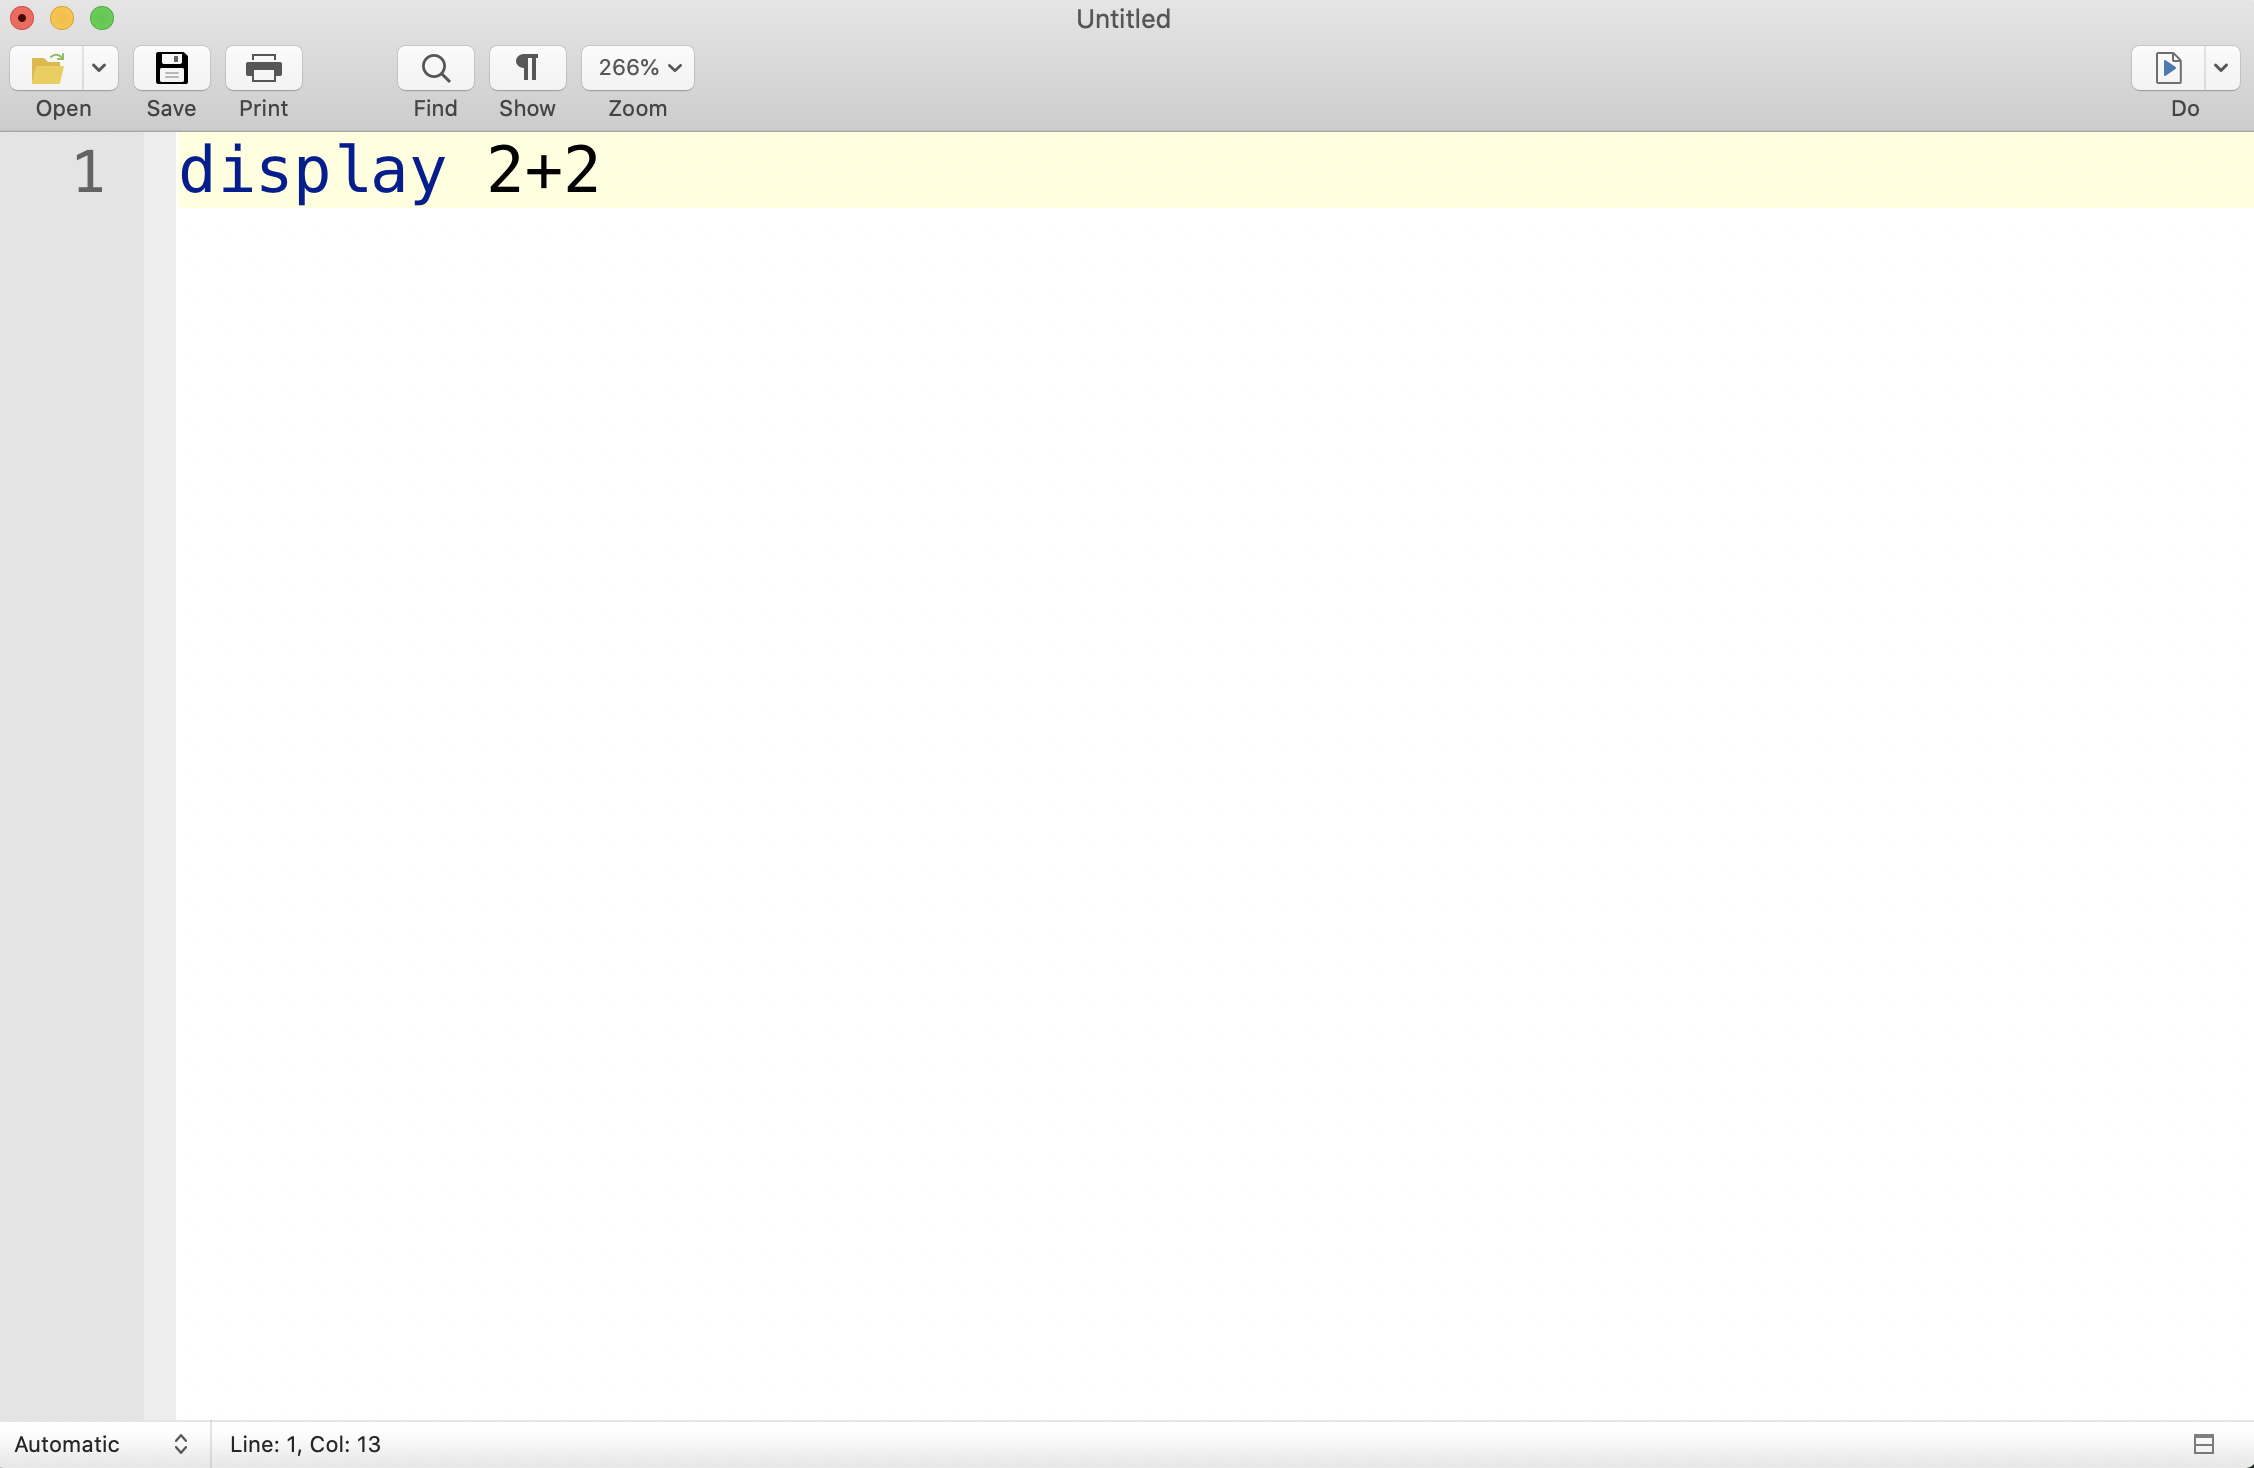
\includegraphics[width=1\linewidth]{images/02_dofile2} 

}

\caption{Display 2+2 in a Do-File}\label{fig:dofile2}
\end{figure}

So now that we have our code written, how do we execute it? There are actually a couple of different ways. The first is pressing the ``Do'' button, which is the icon on the top right of the do-file that looks like a piece of paper with an arrow.

If you press this button without highlighting any text, it will execute every single line of code in the file in the sequence they appear. Depending on your goal, you may want to only run select portions of your code. For example, we often need to ``debug'' our code, and it is more efficient to run a few lines at a time. In this case, we can highlight the lines we would like to be executed, and when we press ``Do'', only the highlighted lines of code will be executed.

For example, in Figure \ref{fig:dofile7}, hitting ``Do'' will execute the first two lines of code.

\begin{figure}

{\centering 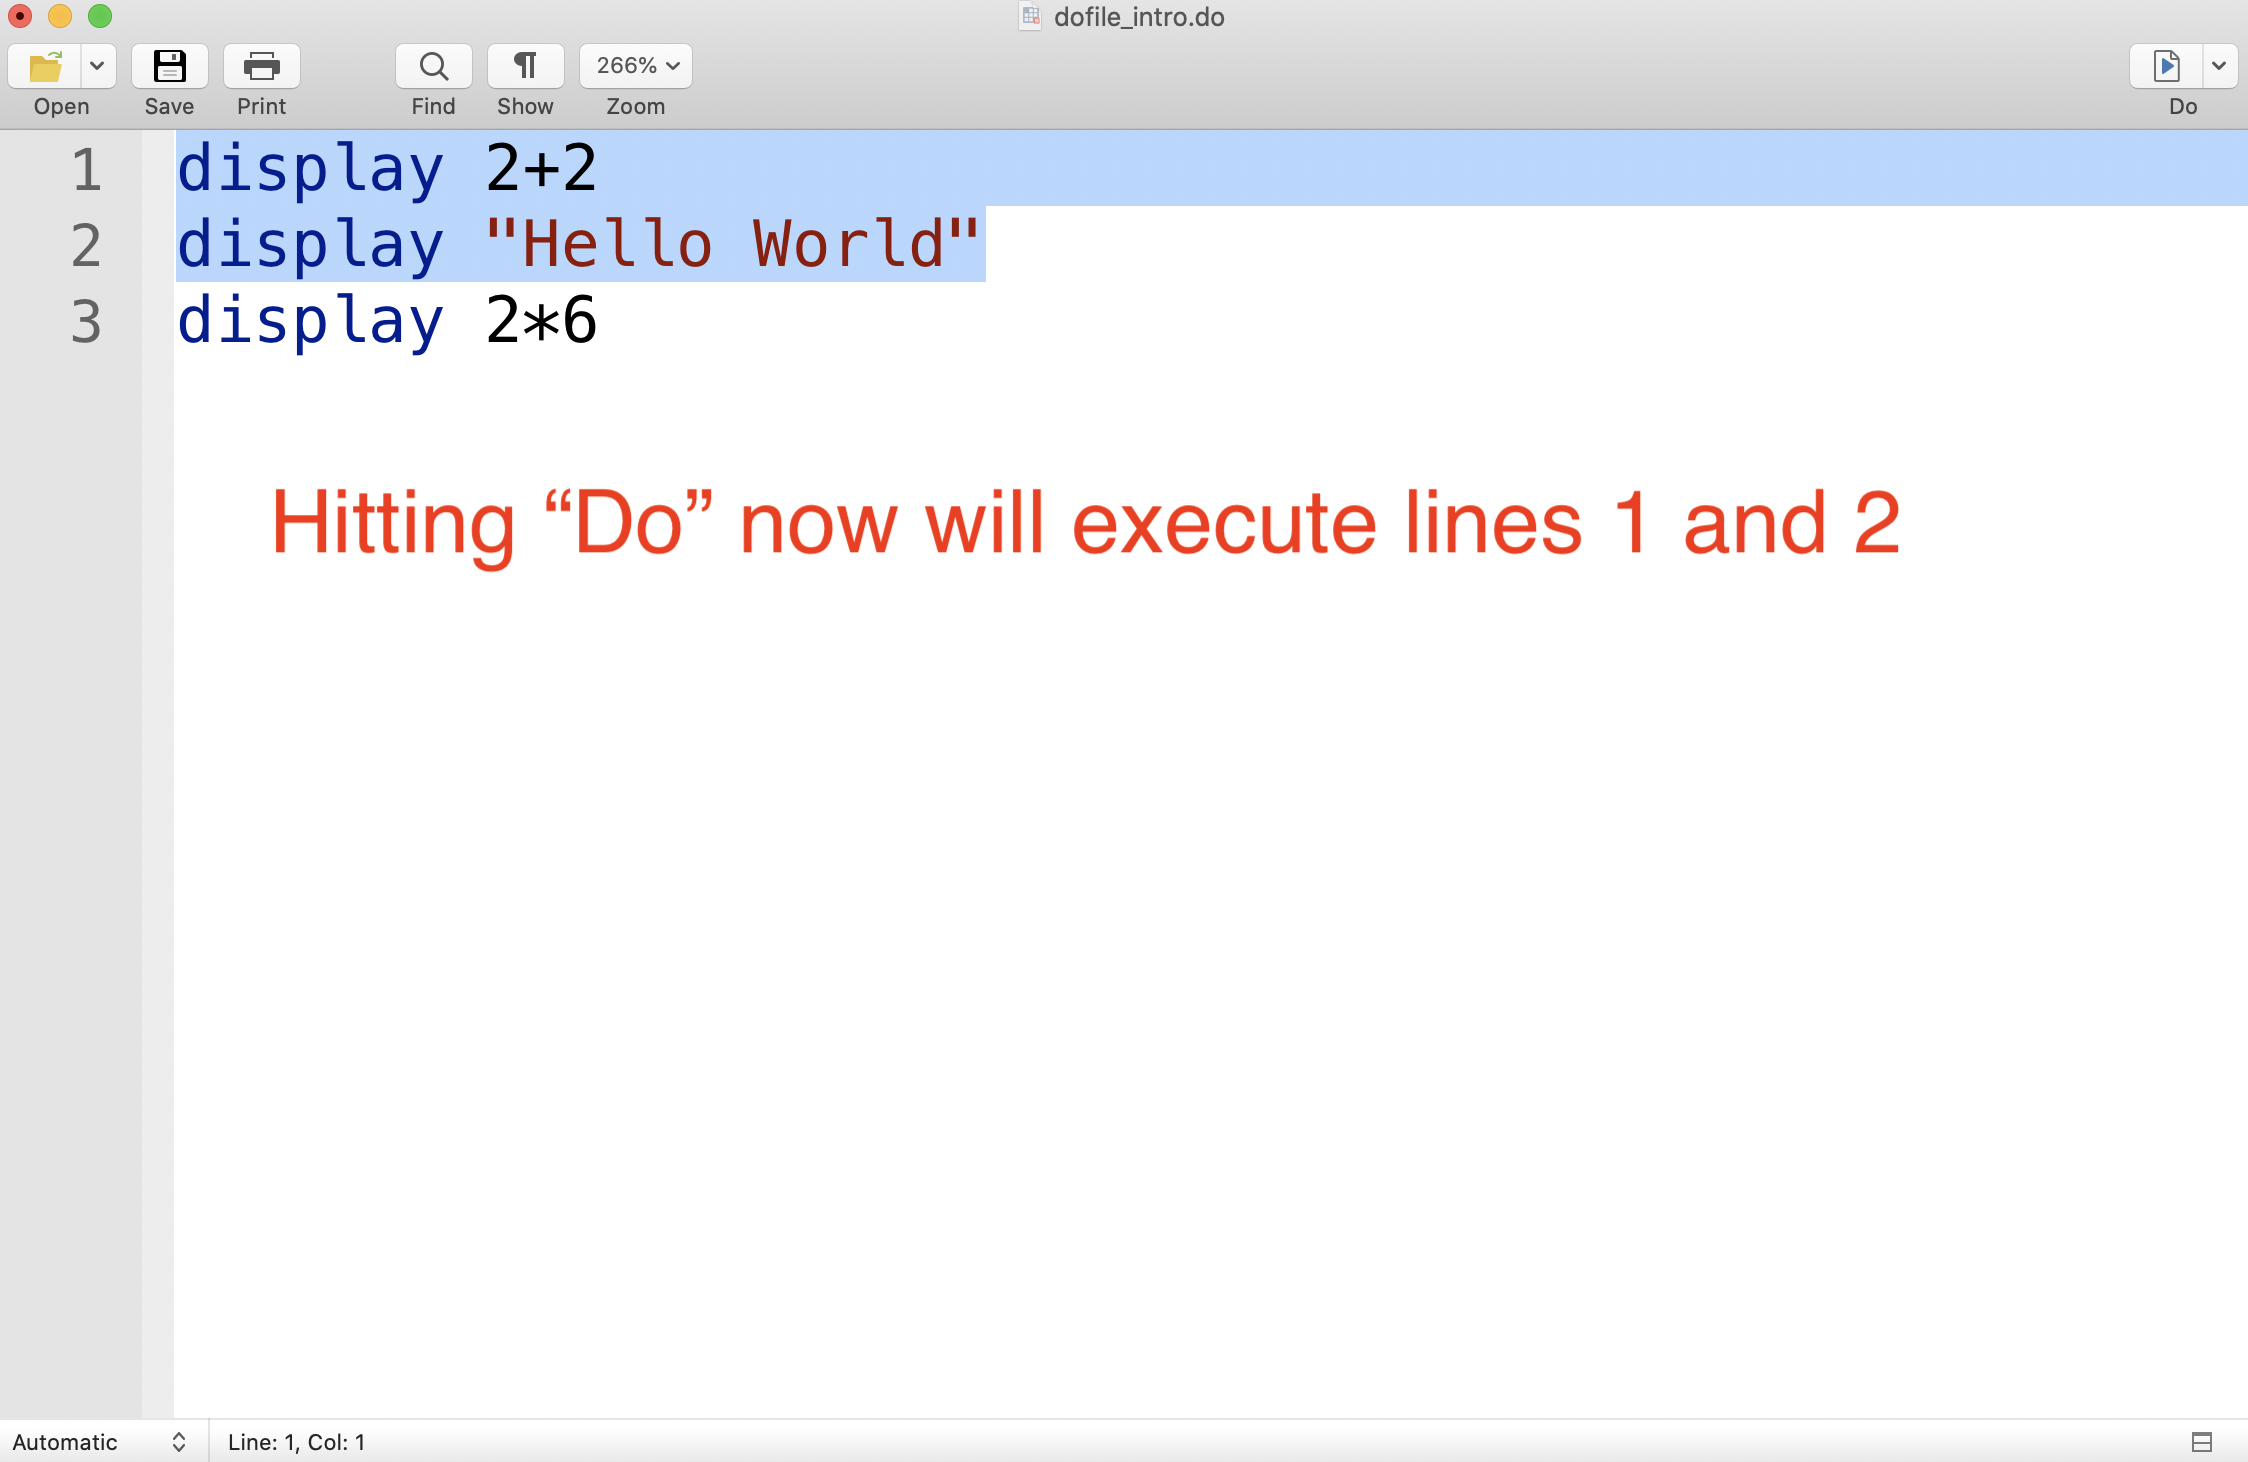
\includegraphics[width=0.75\linewidth]{images/02_dofile7} 

}

\caption{Executing Lines 1 and 2}\label{fig:dofile7}
\end{figure}

In Figure \ref{fig:dofile8}, hitting ``Do'' will execute the second and third line of code.

\begin{figure}

{\centering 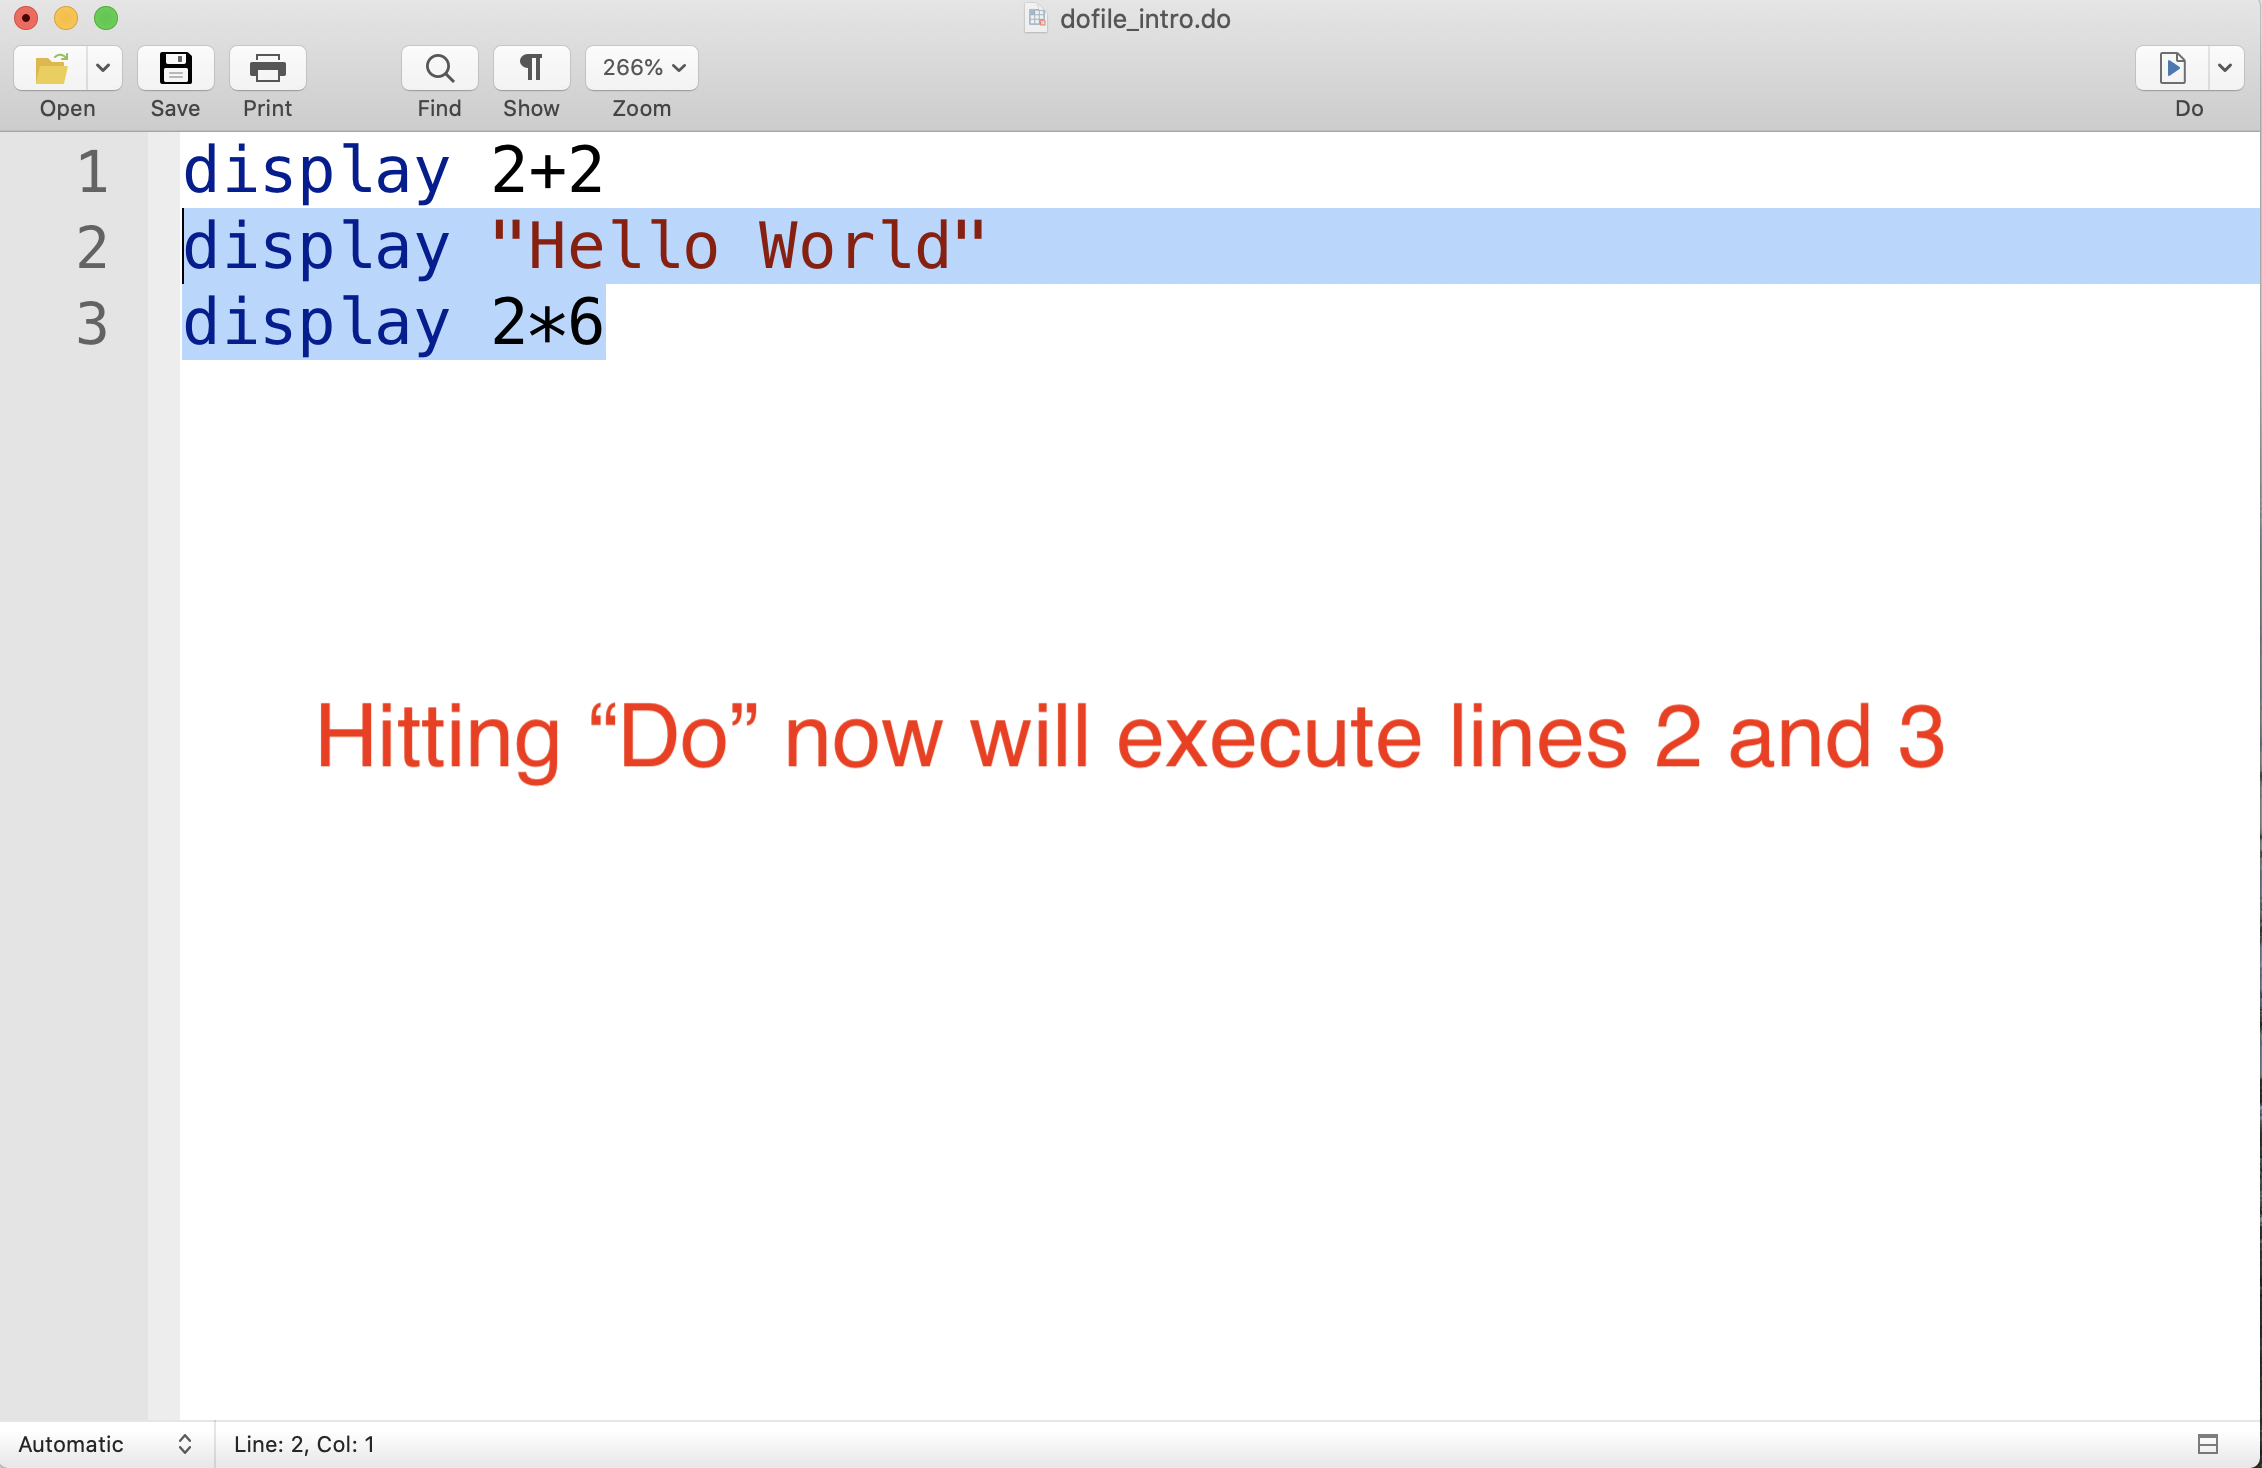
\includegraphics[width=0.75\linewidth]{images/02_dofile8} 

}

\caption{Executing Lines 2 and 3}\label{fig:dofile8}
\end{figure}

We don't actually have to hit ``Do'' to execute the entries of a dofile. Stata does have built-in shortcuts that you can use. A shortcut is a set of keys that you can press in order to perform the same operation as pressing a button. For example, in a Mac, if you press ``Cmd + Shift + D'' when highlighting sections of code, the highlighted sections will be executed. On a PC, the shortcut is ``Ctrl + D''.

Lastly, the key aspect of do-file is that you can save your progress. For example, if you do a homework assignment in multiple sittings, you better have a way to start where you left off! To save a do-file press the ``Save'' button in the top left corner of the page, as seen in Figure \ref{fig:dofile5}

\begin{figure}

{\centering 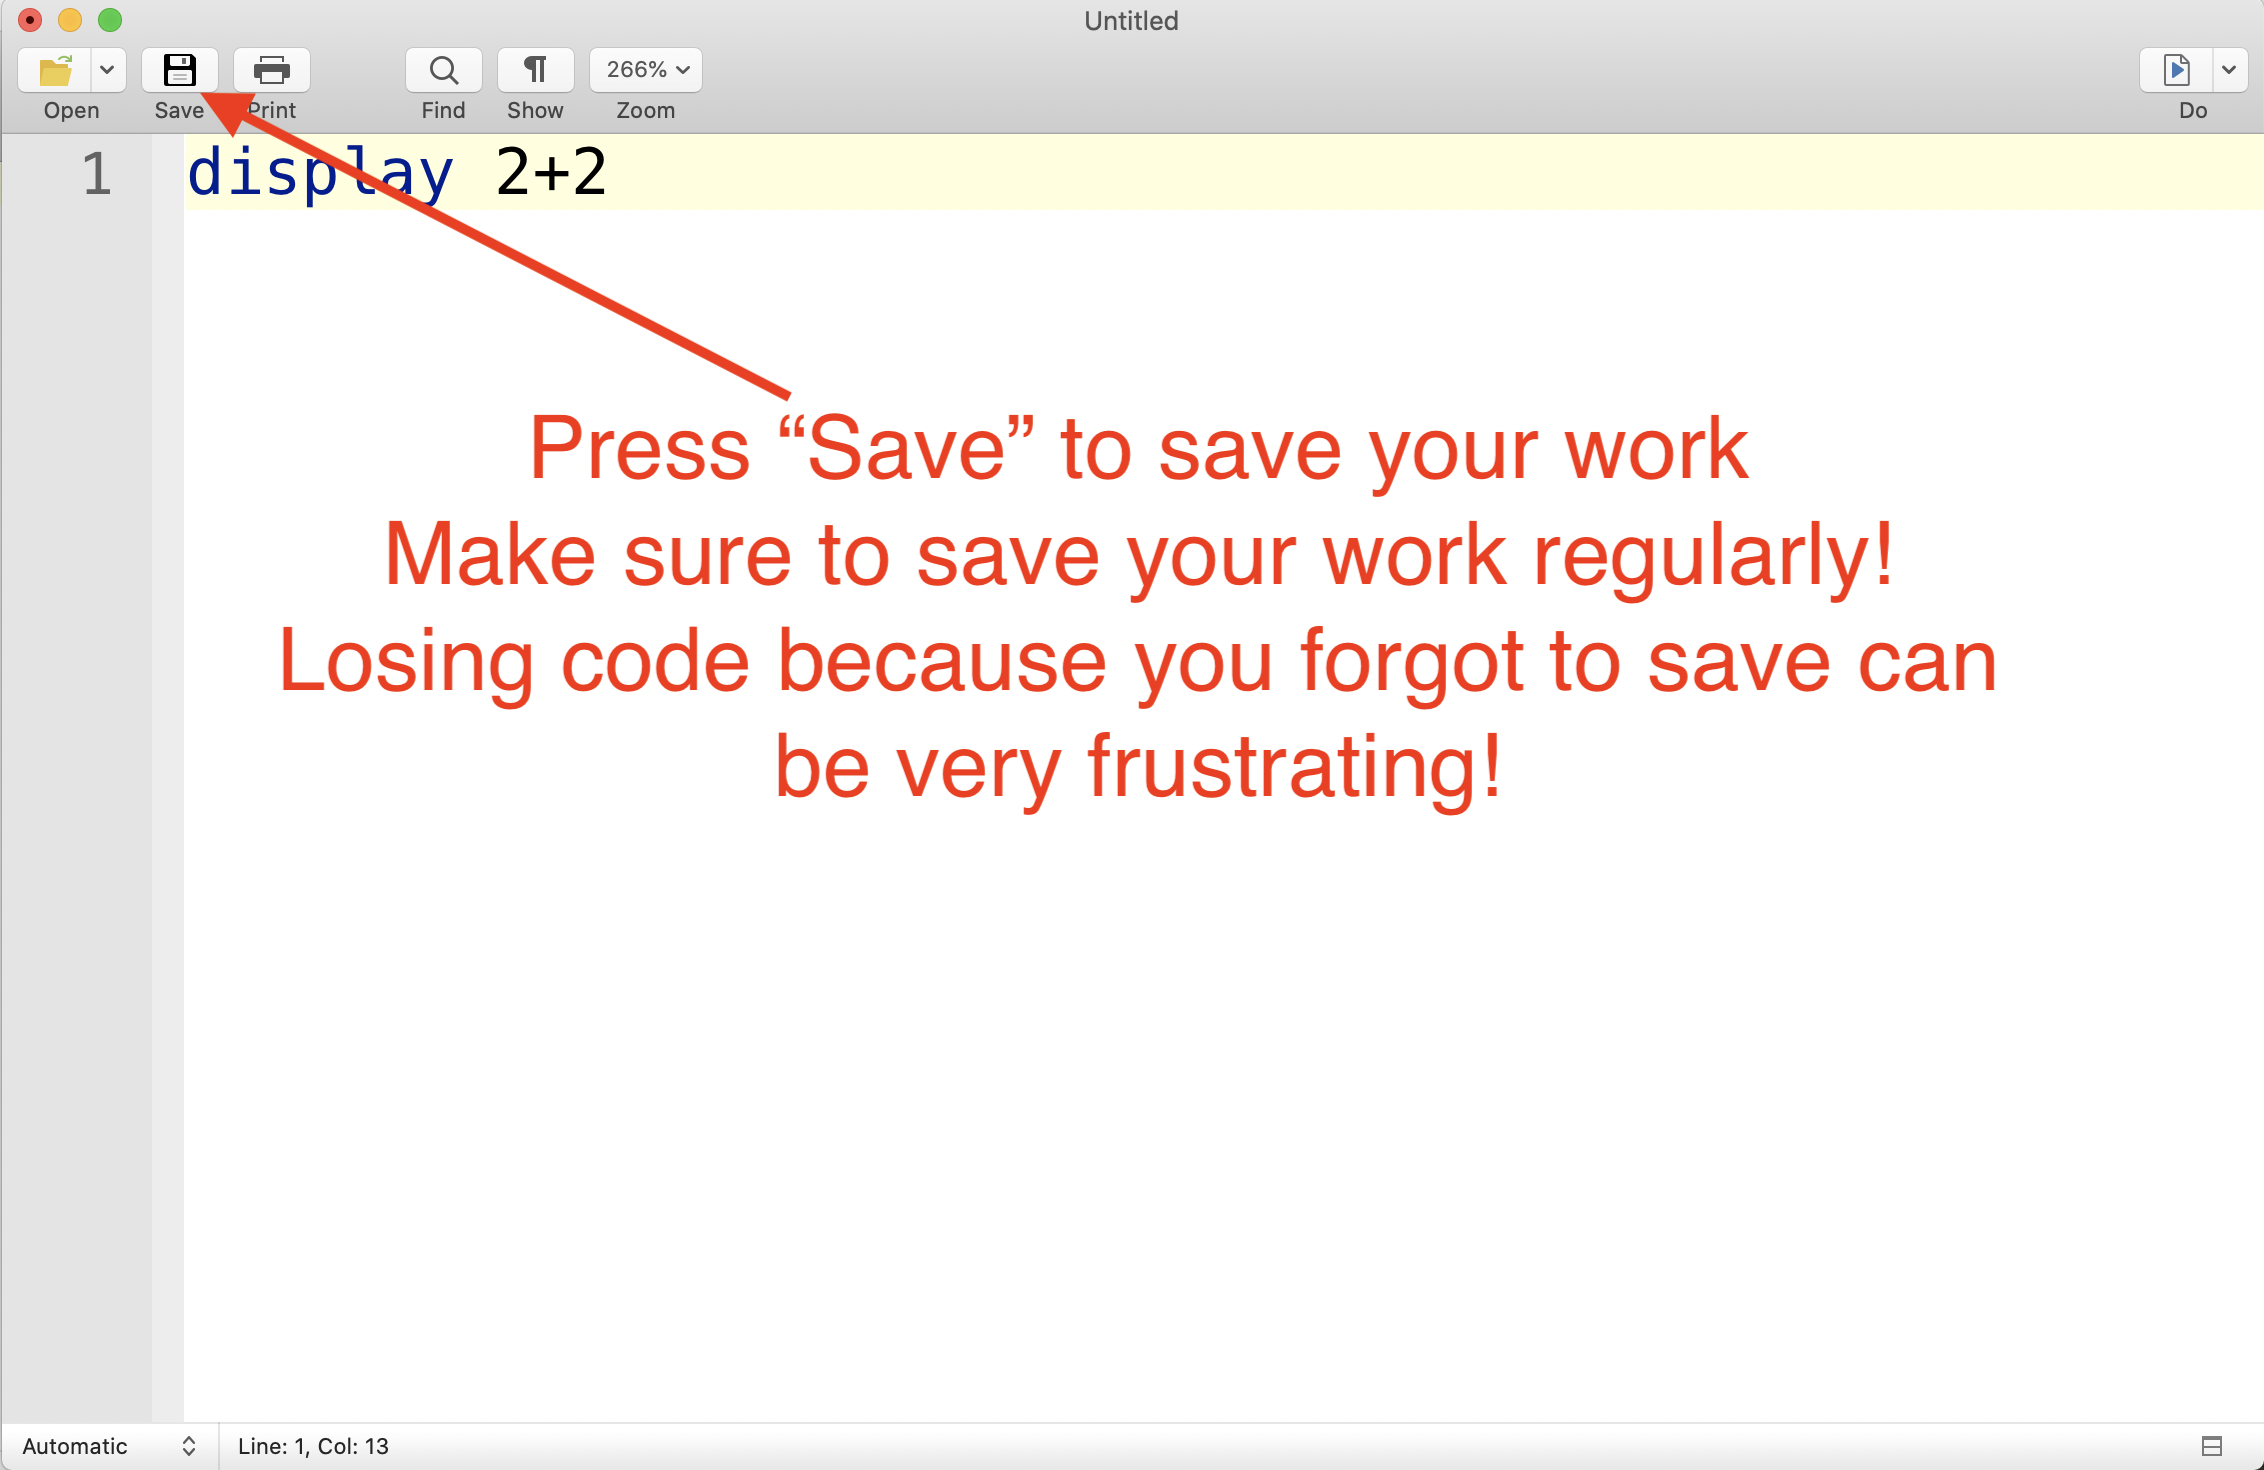
\includegraphics[width=0.75\linewidth]{images/02_dofile4} 

}

\caption{Saving A Do-File}\label{fig:dofile5}
\end{figure}

You should save the do-file somewhere convenient on your computer so that you can quickly find it next time you need it.

\section{Working Directory}\label{working-directory}

Next, we are going to discuss the working directory. To understand the working directory, you first need to understand that every file and folder on your computer has an ``address'' associated with it. Most of us are used to navigating through either Finder on a Mac or through File Explorer on a PC to open a file we need.

But this is not the only way to open files. In fact, originally, there was no convenient user interface in computers to access files in this way. Instead, you needed to direct your computer to the location of the file by typing in the file's ``address''. The ``address'' of a file or folder is known as the \textbf{path name}. It is a string of text that tells your computer where the file or folder is located.

The \textbf{working directory} is the default path in Stata. This is where Stata looks for files by default. For example, imagine I have a dataset named, ``interesting\_data.dta'' and I want to load it into Stata. The command to load data in Stata is the \texttt{use} command. Therefore, I might want to type:

\begin{Shaded}
\begin{Highlighting}[]
\KeywordTok{use}\NormalTok{ interesting\_data.dta, }\KeywordTok{clear}
\end{Highlighting}
\end{Shaded}

The \texttt{,\ clear} tells Stata to clear out any data that is currently loaded into memory. Where will Stata look for the file ``interesting\_data.dta''? In the working directory!

Therefore, before you start loading in data, you need to learn what your working directory is currently set to. To check this in Stata, we use the \texttt{pwd} command, which is short for ``print working directory''. To check your working directory in Stata, just type \texttt{pwd} into the command window. When I typed this into my command window, this is the path name that came out:

\texttt{/Users/davidarnold/Documents/Stata}

This will not be a convenient folder for our working directory. We want the working directory to be set to the place where we put the data after downloading it. For me, this folder is ``/Users/davidarnold/Dropbox/Teaching/EP5/online/02\_week/data''.

For this course, I would suggest creating a folder dedicated to this course. For me, this Folder is on my Dropbox and located within the ``Teaching'' folder. I named my folder for this course ``EP5'', but you can name yours whatever you like.

Additionally, given the large number of datasets we will be using, it will be convenient to separate them somehow. I have divided the course into weeks. Given this application corresponds to the second week, I have named the folder ``02\_week''. Lastly, inside this folder I want to quickly understand where my data is, therefore, I have a dedicated data folder that holds all the datasets we will explore this week.

The structure described above is displayed below in Figure \ref{fig:hierarchy}

\begin{figure}

{\centering 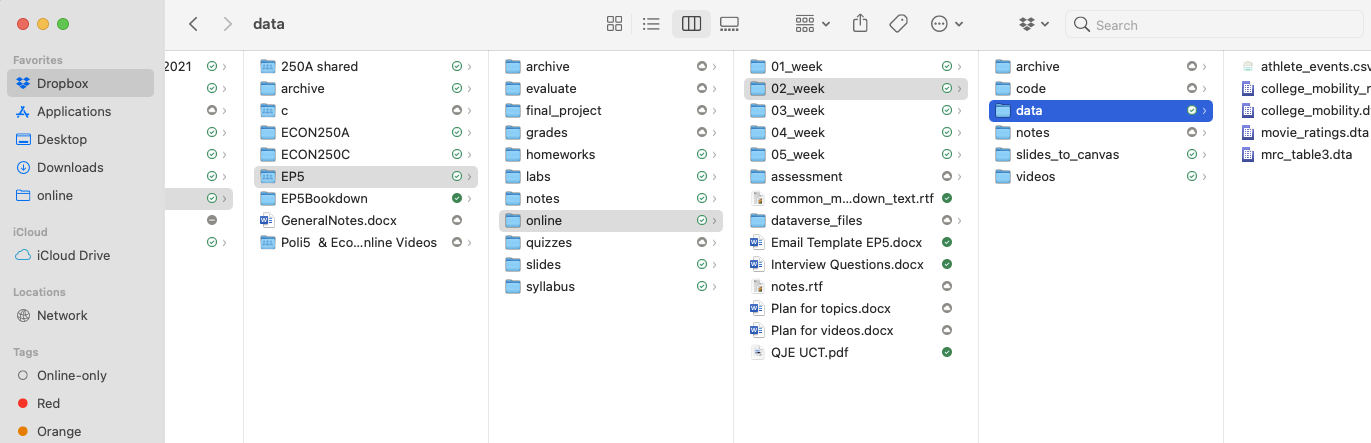
\includegraphics[width=1\linewidth]{images/02_hierarchy} 

}

\caption{Example Structure of a Folder Hierarchy for this Course}\label{fig:hierarchy}
\end{figure}

One brief aside before we continue with understanding the working directory. The best time to organize the folders on your computer is now! What does this mean? It means do not place everything you download in one place. Do not have your desktop cluttered with numerous files. Create folders on your computer that neatly divide up your work. For me, this means different folders for Research and Teaching. Within Teaching, I need different folders for every course I teach. Within each course, I need different folders for every week of the course. Therefore, if I need to access a dataset or set of notes for a given week of the course, I can do so quickly and easily. Doing this organization now will save you a lot of time in the future, not just in this course, but even more generally.

Returning to the working directory, now that we know where the data is, we need to change our directory to the location of the data. To do this we can use the \texttt{cd} command which is short for ``change directory.''

\begin{Shaded}
\begin{Highlighting}[]
\NormalTok{cd }\StringTok{"/Users/davidarnold/Dropbox/Teaching/EP5/online/02\_week/data"}
\NormalTok{file gapminder.dta }\KeywordTok{not}\NormalTok{ Stata }\KeywordTok{format}
\FunctionTok{r}\NormalTok{(610);}


\NormalTok{/Users/davidarnold/Dropbox/Teaching/EP5/online/02\_week/}\KeywordTok{data}
\end{Highlighting}
\end{Shaded}

This is the path for me, but it will be different depending on where you put the downloaded data for this section. One issue that commonly confuses students is that even though they can navigate to a file, they don't actually know the full path to that file.

In a PC, retrieving the full path is relatively simple. In the file explorer, there will be a panel at the top that shows the different subfolders. Clicking on the arrow next to this path will convert it to the full path name. You can simply copy and paste this pathname into Stata to change your working directory.

On a Mac, it is slightly more complicated. If you right-click a folder and then press the ``option'' key, there will be an option to ``copy as pathname''. Pressing this option will copy the path name for you (i.e.~you can press Cmd+p to paste it, or right-click and then select paste.)

\section{Describe and Browse}\label{describe-and-browse}

In this section, we are going to learn a few basics of loading data into Stata. To get started, let's load in the main data for this chapter, which contains data from Opportunity Insights that will allow us how colleges vary in the extent that they promote intergenerational mobility. To load in the data type:

\begin{Shaded}
\begin{Highlighting}[]
\NormalTok{cd }\StringTok{"/Users/davidarnold/Dropbox/Teaching/EP5/online/02\_week/data"}
\KeywordTok{use}\NormalTok{ college\_mobility.dta, }\KeywordTok{clear}
\NormalTok{file gapminder.dta }\KeywordTok{not}\NormalTok{ Stata }\KeywordTok{format}
\FunctionTok{r}\NormalTok{(610);}


\NormalTok{/Users/davidarnold/Dropbox/Teaching/EP5/online/02\_week/}\KeywordTok{data}

\NormalTok{(Preferred Estimates }\KeywordTok{of}\NormalTok{ Access and Mobility Rates }\KeywordTok{by}\NormalTok{ College)}
\end{Highlighting}
\end{Shaded}

Again, the first part of this code (the part following ``cd'') will look different for you depending on the path to data in your computer. Now the data has been loaded into memory, but don't yet understand what is actually in the data. The first command that can be used to start exploring the data is the \texttt{describe} command. The \texttt{describe} command allows us to quickly review the variables in a dataset.

\begin{Shaded}
\begin{Highlighting}[]
\KeywordTok{describe}
\end{Highlighting}
\end{Shaded}

Figure \ref{fig:describe} displays the results of this command, which is a table of variables, as well as the format of the variable and the label associated with the variable.

\begin{figure}

{\centering 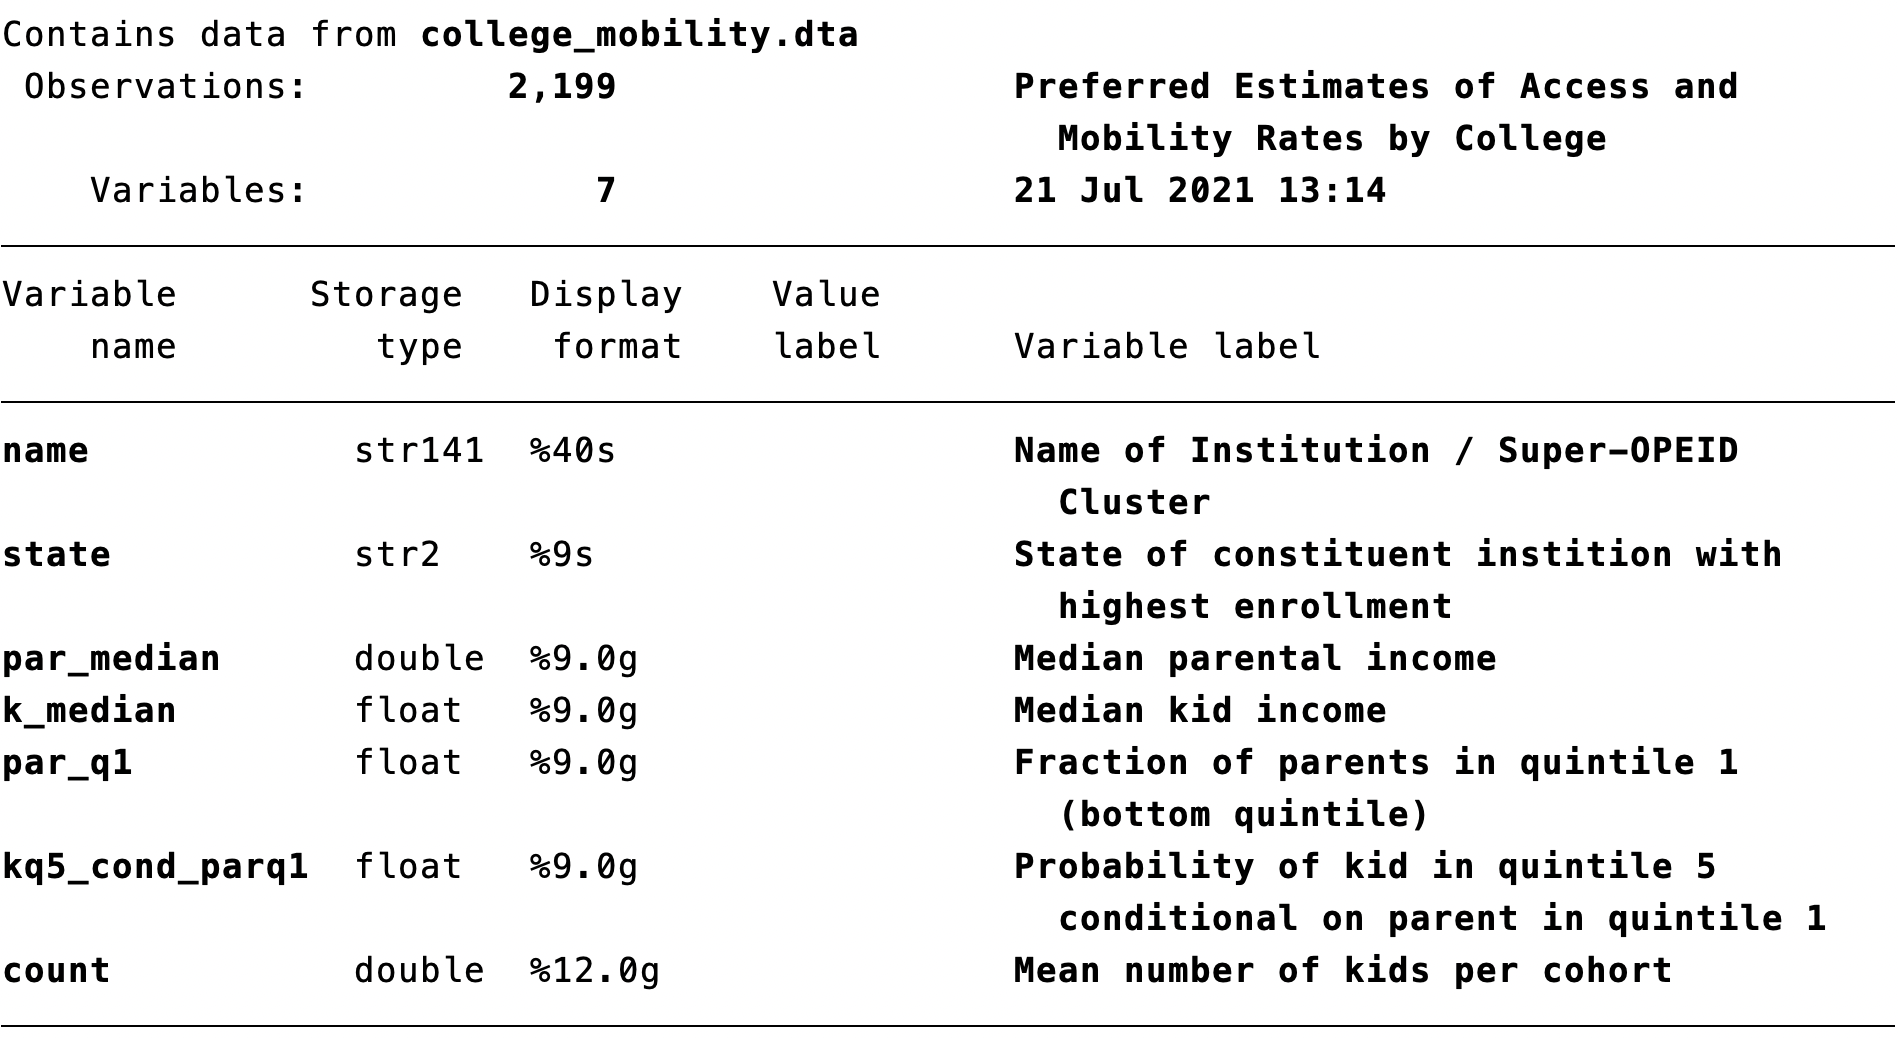
\includegraphics[width=1\linewidth]{images/02_describe_ex} 

}

\caption{Describe Command}\label{fig:describe}
\end{figure}

Here we can note a few of the more important variables we will be using in this dataset. First, we have the variable \texttt{name} which indicates the institution. This is a dataset of 2,199 institutions in the United States. The variables we will focus on are \texttt{par\_q1} and \texttt{kq5\_cond\_parq1}. The label associated with \texttt{par\_q1} is ``Fraction of parents in quintile 1 (bottom quintile)''. In terms of our definition of mobility rate, this is the access portion. A school that has a large fraction of students from the bottom 20 percent of the income distribution (quintile 1) will have high access.

The other component of the mobility rate is the success rate, which is captured by the variable \texttt{kq5\_cond\_parq1}. The label associated with this variable is ``Probability of kid in quintile 5 conditional on parent in quintile 1''. In other words, what fraction of students from low-income backgrounds go on to earn in the top 20 percent of all earners in their age group?

The mobility rate is the product of the access rate and success rate. As we can see, this variable is not in our dataset, so we will eventually need to create it.

While the \texttt{describe} command gives us a good sense of what variables are in the data, it is also useful look directly at the data. The \texttt{browse} command opens up a spreadsheet similar to an Excel spreadsheet. This allows you to look through the data to further understand how the values of each variable are stored. To browse the data, simply type into the command window:

\begin{Shaded}
\begin{Highlighting}[]
\NormalTok{browse}
\end{Highlighting}
\end{Shaded}

For our dataset, this will open the data table displayed in Figure \ref{fig:browseex}

\begin{figure}

{\centering 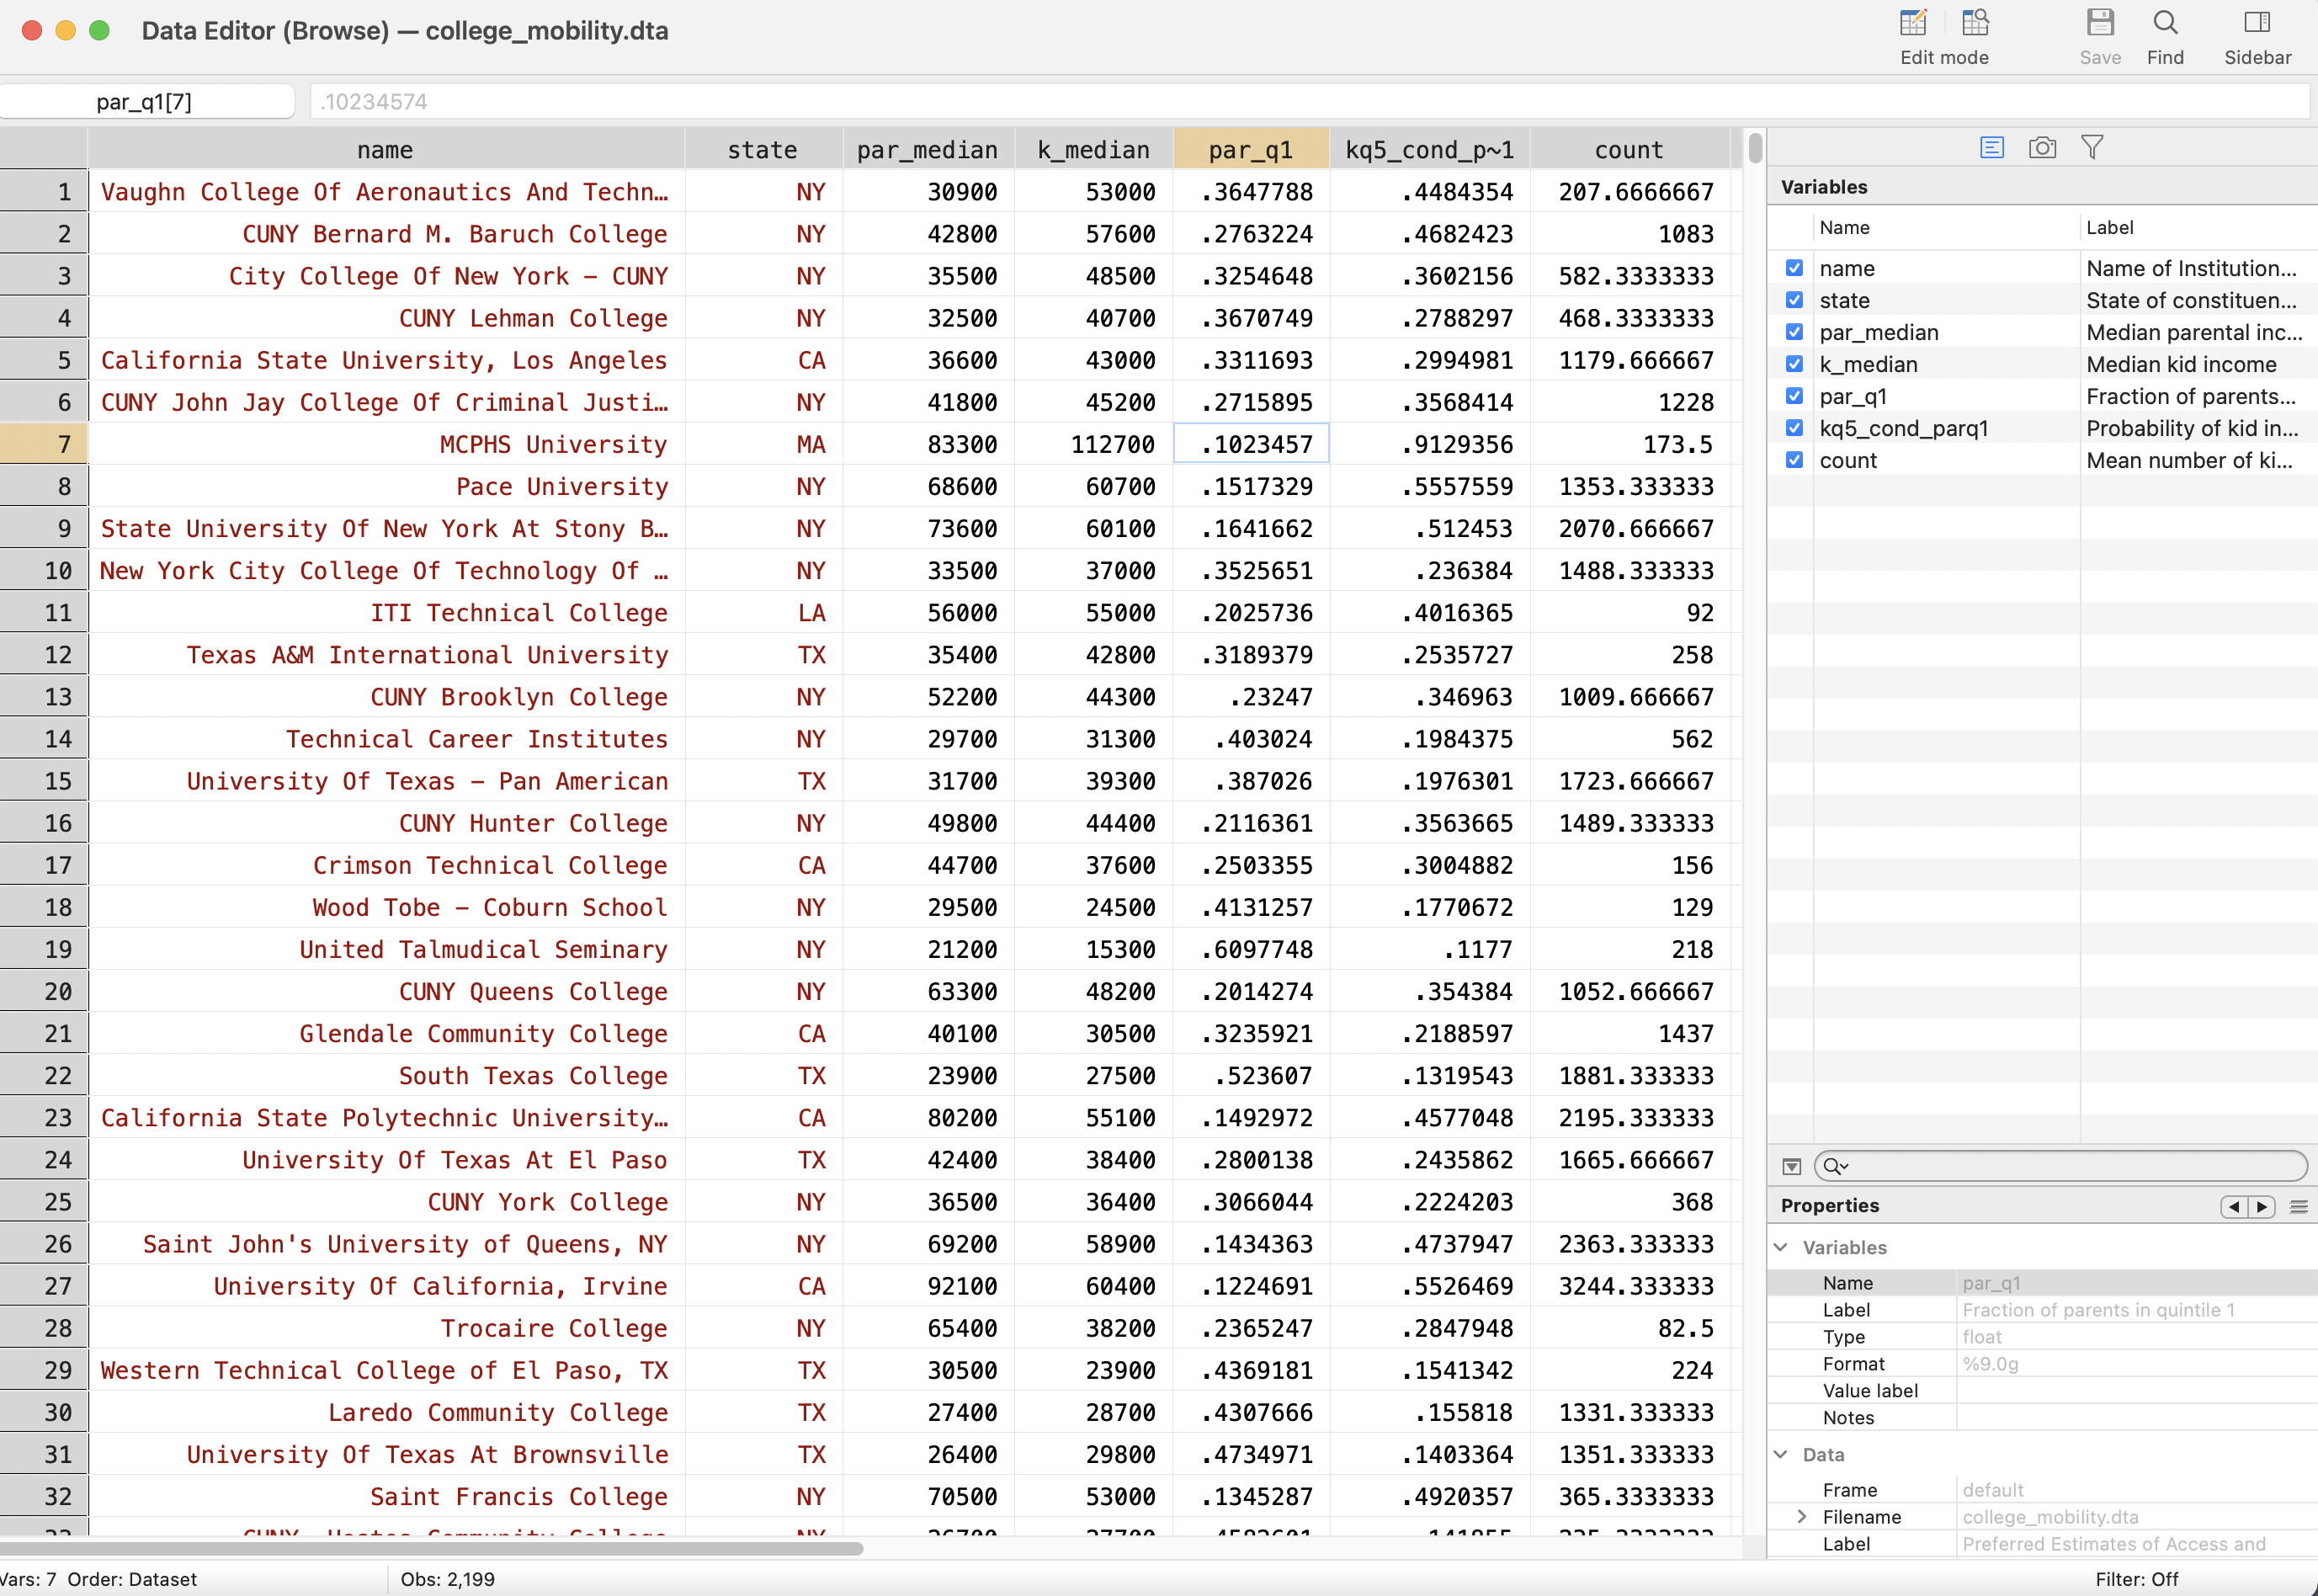
\includegraphics[width=1\linewidth]{images/02_browse_ex} 

}

\caption{Browse Command}\label{fig:browseex}
\end{figure}

When you open a new dataset it is often helpful for us to browse the data. For example, now we know exactly how the \texttt{state} variable is stored (as abbreviations rather than full names). We can also see clearly in the data table which variables are stored as strings and which variables are stored as numbers.

String variables are highlighted in red. Numeric variables are stored in black. Sometimes a variable may seem like it should be a numeric variable, but will contain non-numeric strings. For example, a value of ``\$24,000'' will be stored as a string because both ``\$'' and ``,'' are non-numeric characters.

\section{Summarize}\label{summarize}

Now that we have a sense of our variables, let's generate some descriptive statistics to understand them further. A descriptive statistic is any statistic that quantitatively describes the variable (common ones are the mean, median, and standard deviation). In Stata, the \texttt{summarize} command is useful for retrieving summary statistics

The basic syntax for the \texttt{summarize} command is

\texttt{summarize\ varlist}

where \texttt{varlist} is a list of variables that you would like to see summary statistics for. For example, imagine first we want to understand, on average, how large are institutions in this dataset? Well, the variable \texttt{count} is the average number of students enrolled in the institution. To retrieve summary statistics for this variable we type:

\begin{Shaded}
\begin{Highlighting}[]
\KeywordTok{summarize} \FunctionTok{count}
\end{Highlighting}
\end{Shaded}

\begin{Shaded}
\begin{Highlighting}[]
\KeywordTok{summarize} \FunctionTok{count}
\NormalTok{file gapminder.dta }\KeywordTok{not}\NormalTok{ Stata }\KeywordTok{format}
\FunctionTok{r}\NormalTok{(610);}


\NormalTok{no variables defined}
\FunctionTok{r}\NormalTok{(111);}

\FunctionTok{r}\NormalTok{(111);}
\end{Highlighting}
\end{Shaded}

This table tells us a few things. First, it tells us that the average size of a cohort of students across all institutions in the dataset is about 946 students. Additionally, we can see the minimum is 50 and the maximum is 26989.67. The minimum being 50 is actually by construction. Institutions with less than 50 students per cohort were dropped from the dataset. Understanding descriptive statistics about your key variables is important before starting any data analysis.

\section{Generate}\label{generate}

Now that we understand how to explore the data, let's get back to our question of interest: how do colleges vary in the extent that they promote intergenerational mobility? There is just one problem. We don't have mobility rates in our data.

To remind you, the mobility rate of a college is given by:

\[
\text{mobility rate}= \underbrace{\text{(frac. of students from Q1)}}_{\text{Acess}} \; \cdot \; \underbrace{\text{(frac. of Q1 that reach Q5)}}_{\text{Success}} \nonumber
\]

In our dataset, we have variables that capture the access term (\texttt{par\_q1}) and
the success term (\texttt{kq5\_cond\_parq1}). From these we can construct a college's mobility rate. To do this we will use the \texttt{generate} command

The most basic syntax of the generate command is

\begin{Shaded}
\begin{Highlighting}[]
\KeywordTok{gen}\NormalTok{ newvar = }\FunctionTok{exp}
\end{Highlighting}
\end{Shaded}

In this command, \texttt{newvar} is the name of the new variable that you would like to create. You can give the variable any name you like, but generally it is good practice to keep names short, but as descriptive as possible. The term \texttt{exp} is an expression. How you fill in \texttt{exp} depends on what variable you are creating

Before we get to generating mobility rates, let's take some common examples. Suppose we have two variables \texttt{x1} and \texttt{x2} and we want to create new variables that are functions of these two variables. Here are a few examples of what we might want to accomplish

\begin{itemize}
\item
  Addition: \texttt{gen\ sum\ =\ x1+x2}
\item
  Subtraction: \texttt{gen\ diff\ =\ x1-x2}
\item
  Multiplication: \texttt{gen\ mult\ =\ x1*x2}
\item
  Division: \texttt{gen\ div\ =\ x1/x2}
\end{itemize}

For us, we want to create a variable that is the product of \texttt{par\_q1} and \texttt{kq5\_cond\_parq1}. Therefore, we can type:

\begin{Shaded}
\begin{Highlighting}[]
\KeywordTok{gen}\NormalTok{ mobility\_rate = par\_q1*kq5\_cond\_parq1}
\NormalTok{file gapminder.dta }\KeywordTok{not}\NormalTok{ Stata }\KeywordTok{format}
\FunctionTok{r}\NormalTok{(610);}


\NormalTok{par\_q1 }\KeywordTok{not}\NormalTok{ found}
\FunctionTok{r}\NormalTok{(111);}

\FunctionTok{r}\NormalTok{(111);}
\end{Highlighting}
\end{Shaded}

When we create a new variable, it won't by default have a label associated with it. If you are working on a project that has many different variables, it is a good idea to label your variables so that you can remember what they represent at a later date. For example, if we want to give the variable \texttt{mobility\_rate} a label we type:

\begin{Shaded}
\begin{Highlighting}[]
\KeywordTok{label} \KeywordTok{var}\NormalTok{ mobility\_rate }\StringTok{"Mobility rate of institution"}
\end{Highlighting}
\end{Shaded}

\section{Binary Variables}\label{binary-variables}

Most of the binary variables we create in this class will be the result from evaluating a logical statement. To review, a logical statement is any statement that is either true or false. For example, the statement ``College X is in California'' is either true or it is false. For ``UCSD'' this statement is true, while for ``ASU'' this is false.

It is often useful to create binary variables (binary meaning two) in our data based on logical statements. For example, in our data on intergenerational mobility, we might be interested in comparing mobility rates across different regions. For example, maybe we want to compare mobility rates in California to mobility rates in other parts of the country. To do this, we might want to create a binary indicator variable that is equal to 1 if the state is in California and zero otherwise. We can create a binary variable that is equal to 1 if a logical statement is true and zero if false we type

\begin{Shaded}
\begin{Highlighting}[]
\KeywordTok{gen}\NormalTok{ CA = (state==}\StringTok{"CA"}\NormalTok{)}
\end{Highlighting}
\end{Shaded}

The logical statement \texttt{(state=="CA")} is true if the state is in California and false if it is not. Note the double-equals sign \texttt{==}. We use double-equals to test the equality of two things. Additionally, note the quotation marks around \texttt{CA}. Reminder: \texttt{state} is a string variable and we always reference string variables with quotation marks.

This statement mirrors the general syntax of how we can create binary variables in Stata. The general syntax is

\begin{Shaded}
\begin{Highlighting}[]
\KeywordTok{gen}\NormalTok{ newvar = (logical statement)}
\end{Highlighting}
\end{Shaded}

This code will generate a new variable (named \texttt{newvar}) which is equal to 1 if the logical statement in parentheses is true and zero if false.

To check whether the results conform to our expectations we can type \texttt{br\ state\ CA}. Below in Figure \ref{fig:brca} we show a small selection of the data that shows us CA is equal to 1 for colleges in ``CA'' and zero otherwise.

\begin{figure}

{\centering 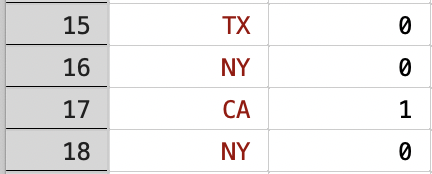
\includegraphics[width=0.6\linewidth]{images/02_br} 

}

\caption{Generating A Binary Indicator for California Colleges}\label{fig:brca}
\end{figure}

There are a few errors that arise enough that it is valuable to go through them now. First, it is common to forgot the ``double equals'' sign, and instead put one equals sign, as below.

\begin{Shaded}
\begin{Highlighting}[]
\KeywordTok{gen}\NormalTok{ CA2 = (state=}\StringTok{"CA"}\NormalTok{)}
\end{Highlighting}
\end{Shaded}

If we execute this code, we will get the error in Figure \ref{fig:forgotdoubleequals}.

\begin{figure}

{\centering 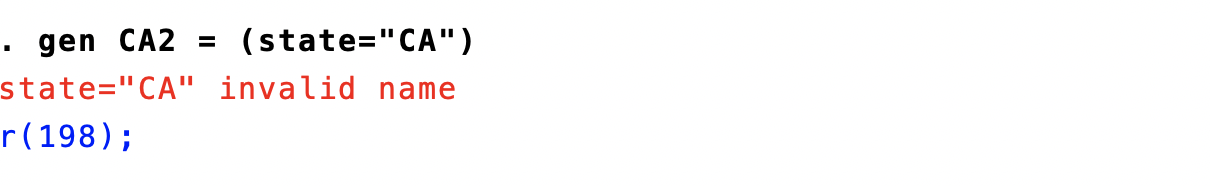
\includegraphics[width=1\linewidth]{images/02_error1} 

}

\caption{Forgetting Double Equals  When Testing Equality}\label{fig:forgotdoubleequals}
\end{figure}

The error report \texttt{state="CA"} is displayed because the command is looking for a variable with this name, which is not in a valid format. To test equality, we need two equals signs.

Another common error (not just when generating new variables) is to forget the quotation marks when referencing string variables. For example if we type:

\begin{Shaded}
\begin{Highlighting}[]
\KeywordTok{gen}\NormalTok{ CA3 = (state==CA)}
\end{Highlighting}
\end{Shaded}

We will get the error code displayed in Figure \ref{fig:forgotquotes}.

\begin{figure}

{\centering 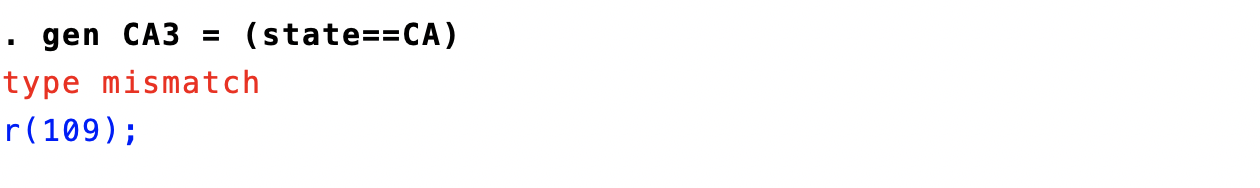
\includegraphics[width=1\linewidth]{images/02_error2} 

}

\caption{Forgetting Quotation Marks When Referencing Strings}\label{fig:forgotquotes}
\end{figure}

The error report \texttt{type\ mismatch} occurs because state is a string variable, yet what comes after the equals sign will NOT be interpreted as a string. To tell Stata the characters \texttt{CA} are strings, put \texttt{CA} in quotation marks!

There are many \texttt{binary} variables we can create from relations. For example, imagine we have two generic variables, \texttt{x1} and \texttt{x2}. We can create a variable that is equal to one if \texttt{x1} is greater than \texttt{x2} and zero otherwise.

\begin{Shaded}
\begin{Highlighting}[]
\KeywordTok{gen}\NormalTok{ x1\_greater\_x2 = (x1\textgreater{}}\KeywordTok{x2}\NormalTok{)}
\end{Highlighting}
\end{Shaded}

A variable that is equal to 1 if \texttt{x1} is less than \texttt{x2} and zero otherwise.

\begin{Shaded}
\begin{Highlighting}[]
\KeywordTok{gen}\NormalTok{ x1\_less\_x2 = (x1\textless{}}\KeywordTok{x2}\NormalTok{)}
\end{Highlighting}
\end{Shaded}

A variable that is equal to 1 if \texttt{x1} is greater than or equal to \texttt{x2} and zero otherwise.

\begin{Shaded}
\begin{Highlighting}[]
\KeywordTok{gen}\NormalTok{ x1\_greater\_x2 = (x1\textgreater{}=}\KeywordTok{x2}\NormalTok{)}
\end{Highlighting}
\end{Shaded}

A variable that is equal to 1 if \texttt{x1} is less than or equal to \texttt{x2} and zero otherwise.

\begin{Shaded}
\begin{Highlighting}[]
\KeywordTok{gen}\NormalTok{ x1\_less\_eq\_x2 = (x1\textless{}=}\KeywordTok{x2}\NormalTok{)}
\end{Highlighting}
\end{Shaded}

\section{If Statements}\label{if-statements}

If statements in Stata are used when you want to execute code, but only if some condition is met. Most of the commands we use in Stata can be combined with an if statement.

The general syntax for using if statements is

\begin{Shaded}
\begin{Highlighting}[]
\NormalTok{command }\KeywordTok{if}\NormalTok{ (logical statement)}
\end{Highlighting}
\end{Shaded}

The command will only be executed for observations for which the logical statement is true. If you look at the help files for commands, you will often notice a \texttt{{[}if{]}} in the syntax. This means you can combine the command with an if statement. For example, in Figure \ref{fig:sumhelp} we can see you can use if statements with the summarize command.

\begin{figure}

{\centering 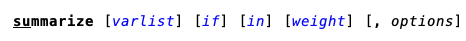
\includegraphics[width=0.75\linewidth]{images/02_sum_help} 

}

\caption{Help File for the Summarize Command}\label{fig:sumhelp}
\end{figure}

A general note about how syntax is presented in Stata is useful here. Words that appear brackets can be used when using the command, but don't need to be. The word \texttt{if} is in brackets because we don't need to include it in order to use the summarize command. However, imagine we want to compute average mobility rates, but just restricted to colleges in California. A college is in California \texttt{if\ CA==1}, which is the binary variable we created before. Therefore we can compute the average mobility rate of California colleges by typing:

\begin{Shaded}
\begin{Highlighting}[]
\KeywordTok{sum}\NormalTok{ mobility\_rate }\KeywordTok{if}\NormalTok{ CA==1 }
\end{Highlighting}
\end{Shaded}

\begin{verbatim}
file gapminder.dta not Stata format
r(610);


no variables defined
r(111);

r(111);
\end{verbatim}

Note that we did not put \texttt{if} in brackets, even though it was in brackets in the syntax. The brackets are there to tell you that you can use an if statement, but the brackets themselves are not actually part of the syntax.

So mobility rates in California colleges are 0.028. Let's compare this number to mobility rates in non-Californian colleges:

\begin{Shaded}
\begin{Highlighting}[]
\KeywordTok{sum}\NormalTok{ mobility\_rate }\KeywordTok{if}\NormalTok{ CA==0 }
\end{Highlighting}
\end{Shaded}

\begin{verbatim}
file gapminder.dta not Stata format
r(610);


no variables defined
r(111);

r(111);
\end{verbatim}

The mobility rates in non-Californian colleges are 0.018, so mobility rates, on average, are higher at Californian schools. Why is this? Well, it could be due to either 2 factors: higher access or higher success. We can check if one vs.~the other is driving this result by summarizing both access and success separately.

\begin{Shaded}
\begin{Highlighting}[]
\KeywordTok{sum}\NormalTok{ par\_q1 kq5\_cond\_parq1 }\KeywordTok{if}\NormalTok{ CA==1 }
\end{Highlighting}
\end{Shaded}

\begin{verbatim}
file gapminder.dta not Stata format
r(610);


no variables defined
r(111);

r(111);
\end{verbatim}

And now for non-Californian colleges:

\begin{Shaded}
\begin{Highlighting}[]
\KeywordTok{sum}\NormalTok{ par\_q1 kq5\_cond\_parq1 }\KeywordTok{if}\NormalTok{ CA==0 }
\end{Highlighting}
\end{Shaded}

\begin{verbatim}
file gapminder.dta not Stata format
r(610);


no variables defined
r(111);

r(111);
\end{verbatim}

So let's first discuss the access results (i.e.~the variable \texttt{par\_q1}). Across colleges in CA, the average fraction of students that are from low-income backgrounds is around 14.4 percent. In contrast, in non-California colleges, the average fraction of students that are from low-income backgrounds is around 12.3 percent. Therefore, on average across schools, access is higher in CA.
Now let's discuss the success results (i.e.~the variable \texttt{kq5\_cond\_parq1}). Across colleges in CA, the average fraction of students from low-income backgrounds that become high earners is around 24.8 percent. Across colleges NOT in CA, the average fraction of students from low-income backgrounds that become high earners is around 19.2 percent. Therefore mobility rates are higher in CA due to both (1) greater access and (2) greater success.

We can also use \texttt{if} statements to reference string variables. For example, let's imagine we want to see what the mobility rate is for UCSD. In the data, we can use the variable \texttt{name} which contains the institution name to summarize mobility \texttt{if\ name\ ==\ "University\ Of\ California,\ San\ Diego"}. Note again the use of quotation marks here to reference a string value.

\begin{Shaded}
\begin{Highlighting}[]
\KeywordTok{sum}\NormalTok{ mobility\_rate }\KeywordTok{if} \BaseNTok{name}\NormalTok{ == }\StringTok{"University Of California, San Diego"}
\end{Highlighting}
\end{Shaded}

\begin{verbatim}
file gapminder.dta not Stata format
r(610);


no variables defined
r(111);

r(111);
\end{verbatim}

Here we have taken the average \texttt{if\ name\ ==\ "University\ Of\ California,\ San\ Diego"}. But only one observation meets this restriction, so the table is just showing us the mobility rate for UCSD, which is equal to 0.048, a bit higher than the average of 0.028 across all Californian institutions.

In this section, we have begun to explore variation across colleges in terms of intergenerational mobility rates. In the next section, we will learn about a data visualization technique that is useful in understanding variation in the data more generally.

\section{Histogram (Theoretical)}\label{histogram-theoretical}

A \textbf{histogram} is a representation of the distribution of a \textbf{numeric} variable \medskip. In our empirical application, we want to understand the distribution of mobility rates across colleges. To keep things simple, let's go through a hypothetical example of a setting you are probably familiar with: understanding the distribution of test scores in a class.

Let's imagine we have a class of 10 students, as depicted below:

\[
  \{65,71,75,76,80,84,85,86,90,98\}
\]

We want to understand the distribution of test scores. To create a histogram, the first thing we must decide is how to ``bin'' our data (sometimes referred to as ``bucket''). Binning the data means to divide the range into a series of intervals. For example, for test scores, I could use the following intervals:

\begin{itemize}
\tightlist
\item
  Interval 1: {[}60,70)
\item
  Interval 2: {[}70,80)
\item
  Interval 3: {[}80,90)
\item
  Interval 4: {[}90,100{]}
\end{itemize}

Reminder: brackets mean inclusive, while parentheses mean excluding. So a score of 70 would fall in interval 2, not 1. Next we compute the fraction of observations within each bin. Only 1 test score (65) falls within interval 1, so 10 percent of observations are in interval 1. Three test scores fall within interval 2, so 30 percent of observations are in interval 2. We can compute the fraction in each interval and then plot the result in a histogram, as depicted in Figure \ref{fig:histtestscore}.

\begin{figure}

{\centering 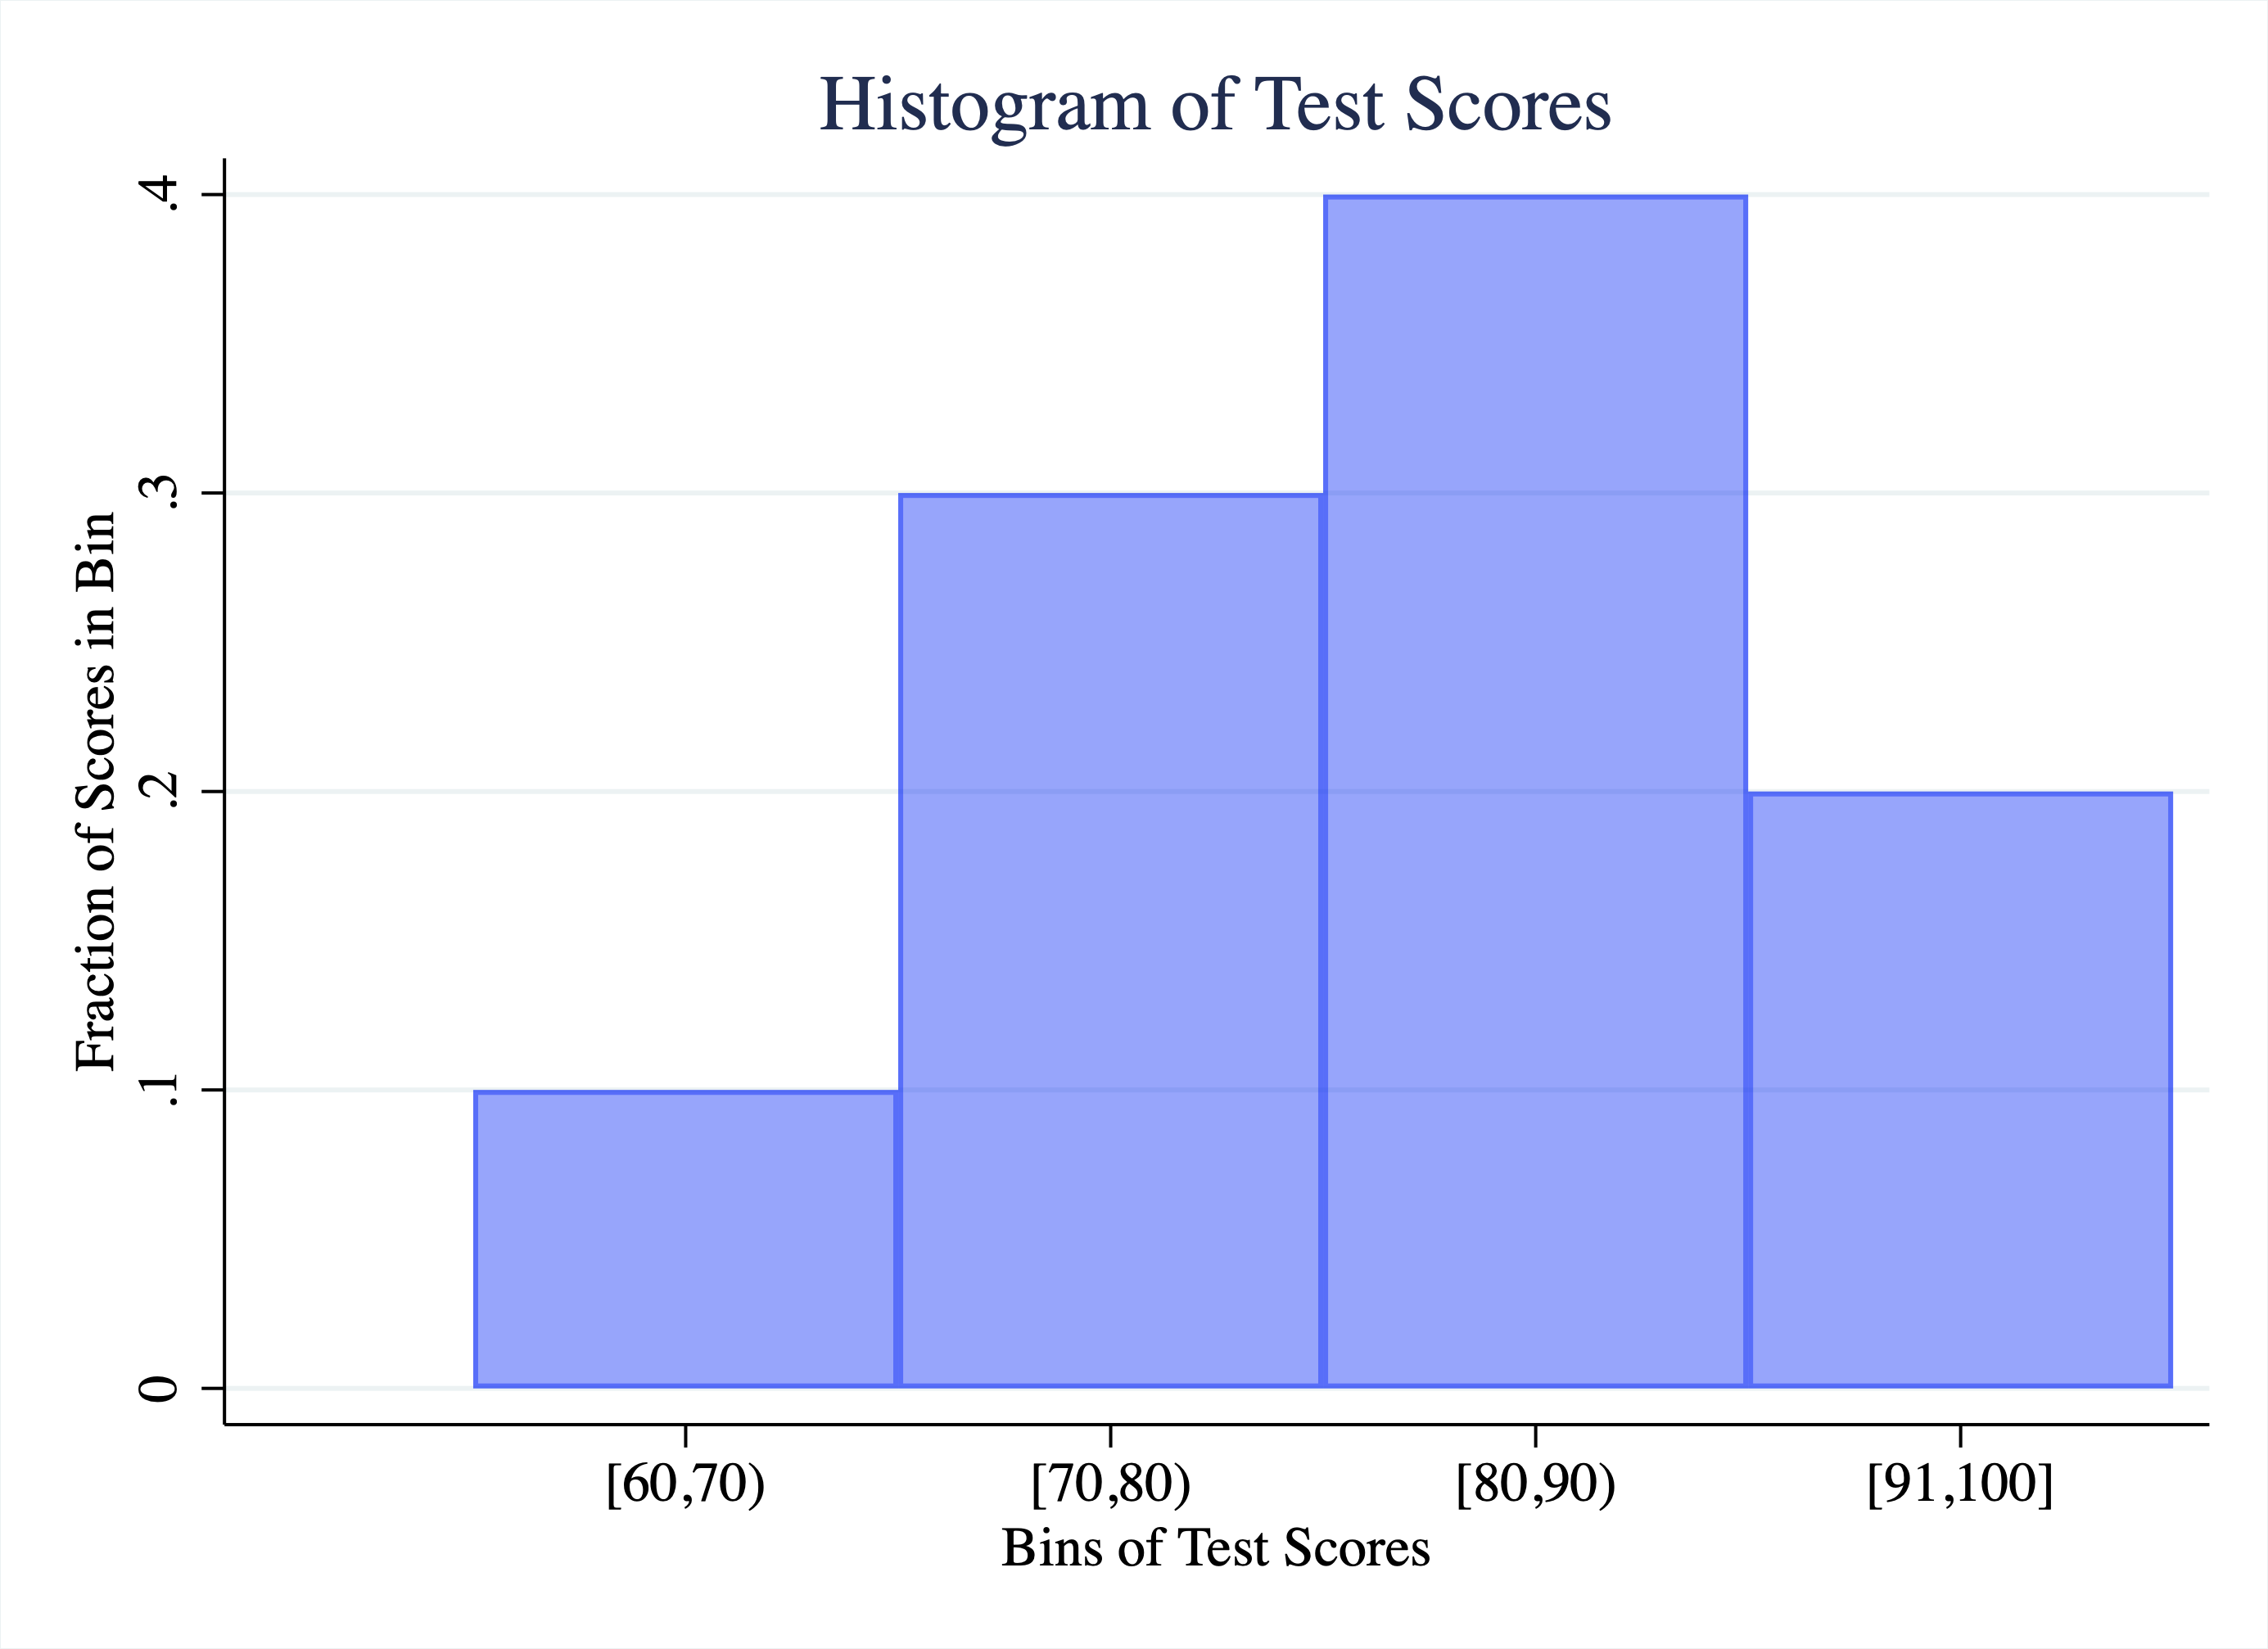
\includegraphics[width=0.75\linewidth]{images/02_hist_ex} 

}

\caption{Histogram of Test Scores}\label{fig:histtestscore}
\end{figure}

So in a histogram, the height of the bar represents what fraction of test scores fall within a given interval. Now that we understand the basic premise, let's go through a few examples from some real datasets.

For example 1 we are going to look at the distribution of Rotten Tomatoes scores for movies released in 2015 in Figure \ref{fig:histmovies}. The rotten tomato score represents what fraction of critics rated a film as positive. So a value of 50 indicates that 50 percent of critics rated the movie positively. The score ranges from a minimum of 0 to a maximum of 100.

\begin{figure}

{\centering 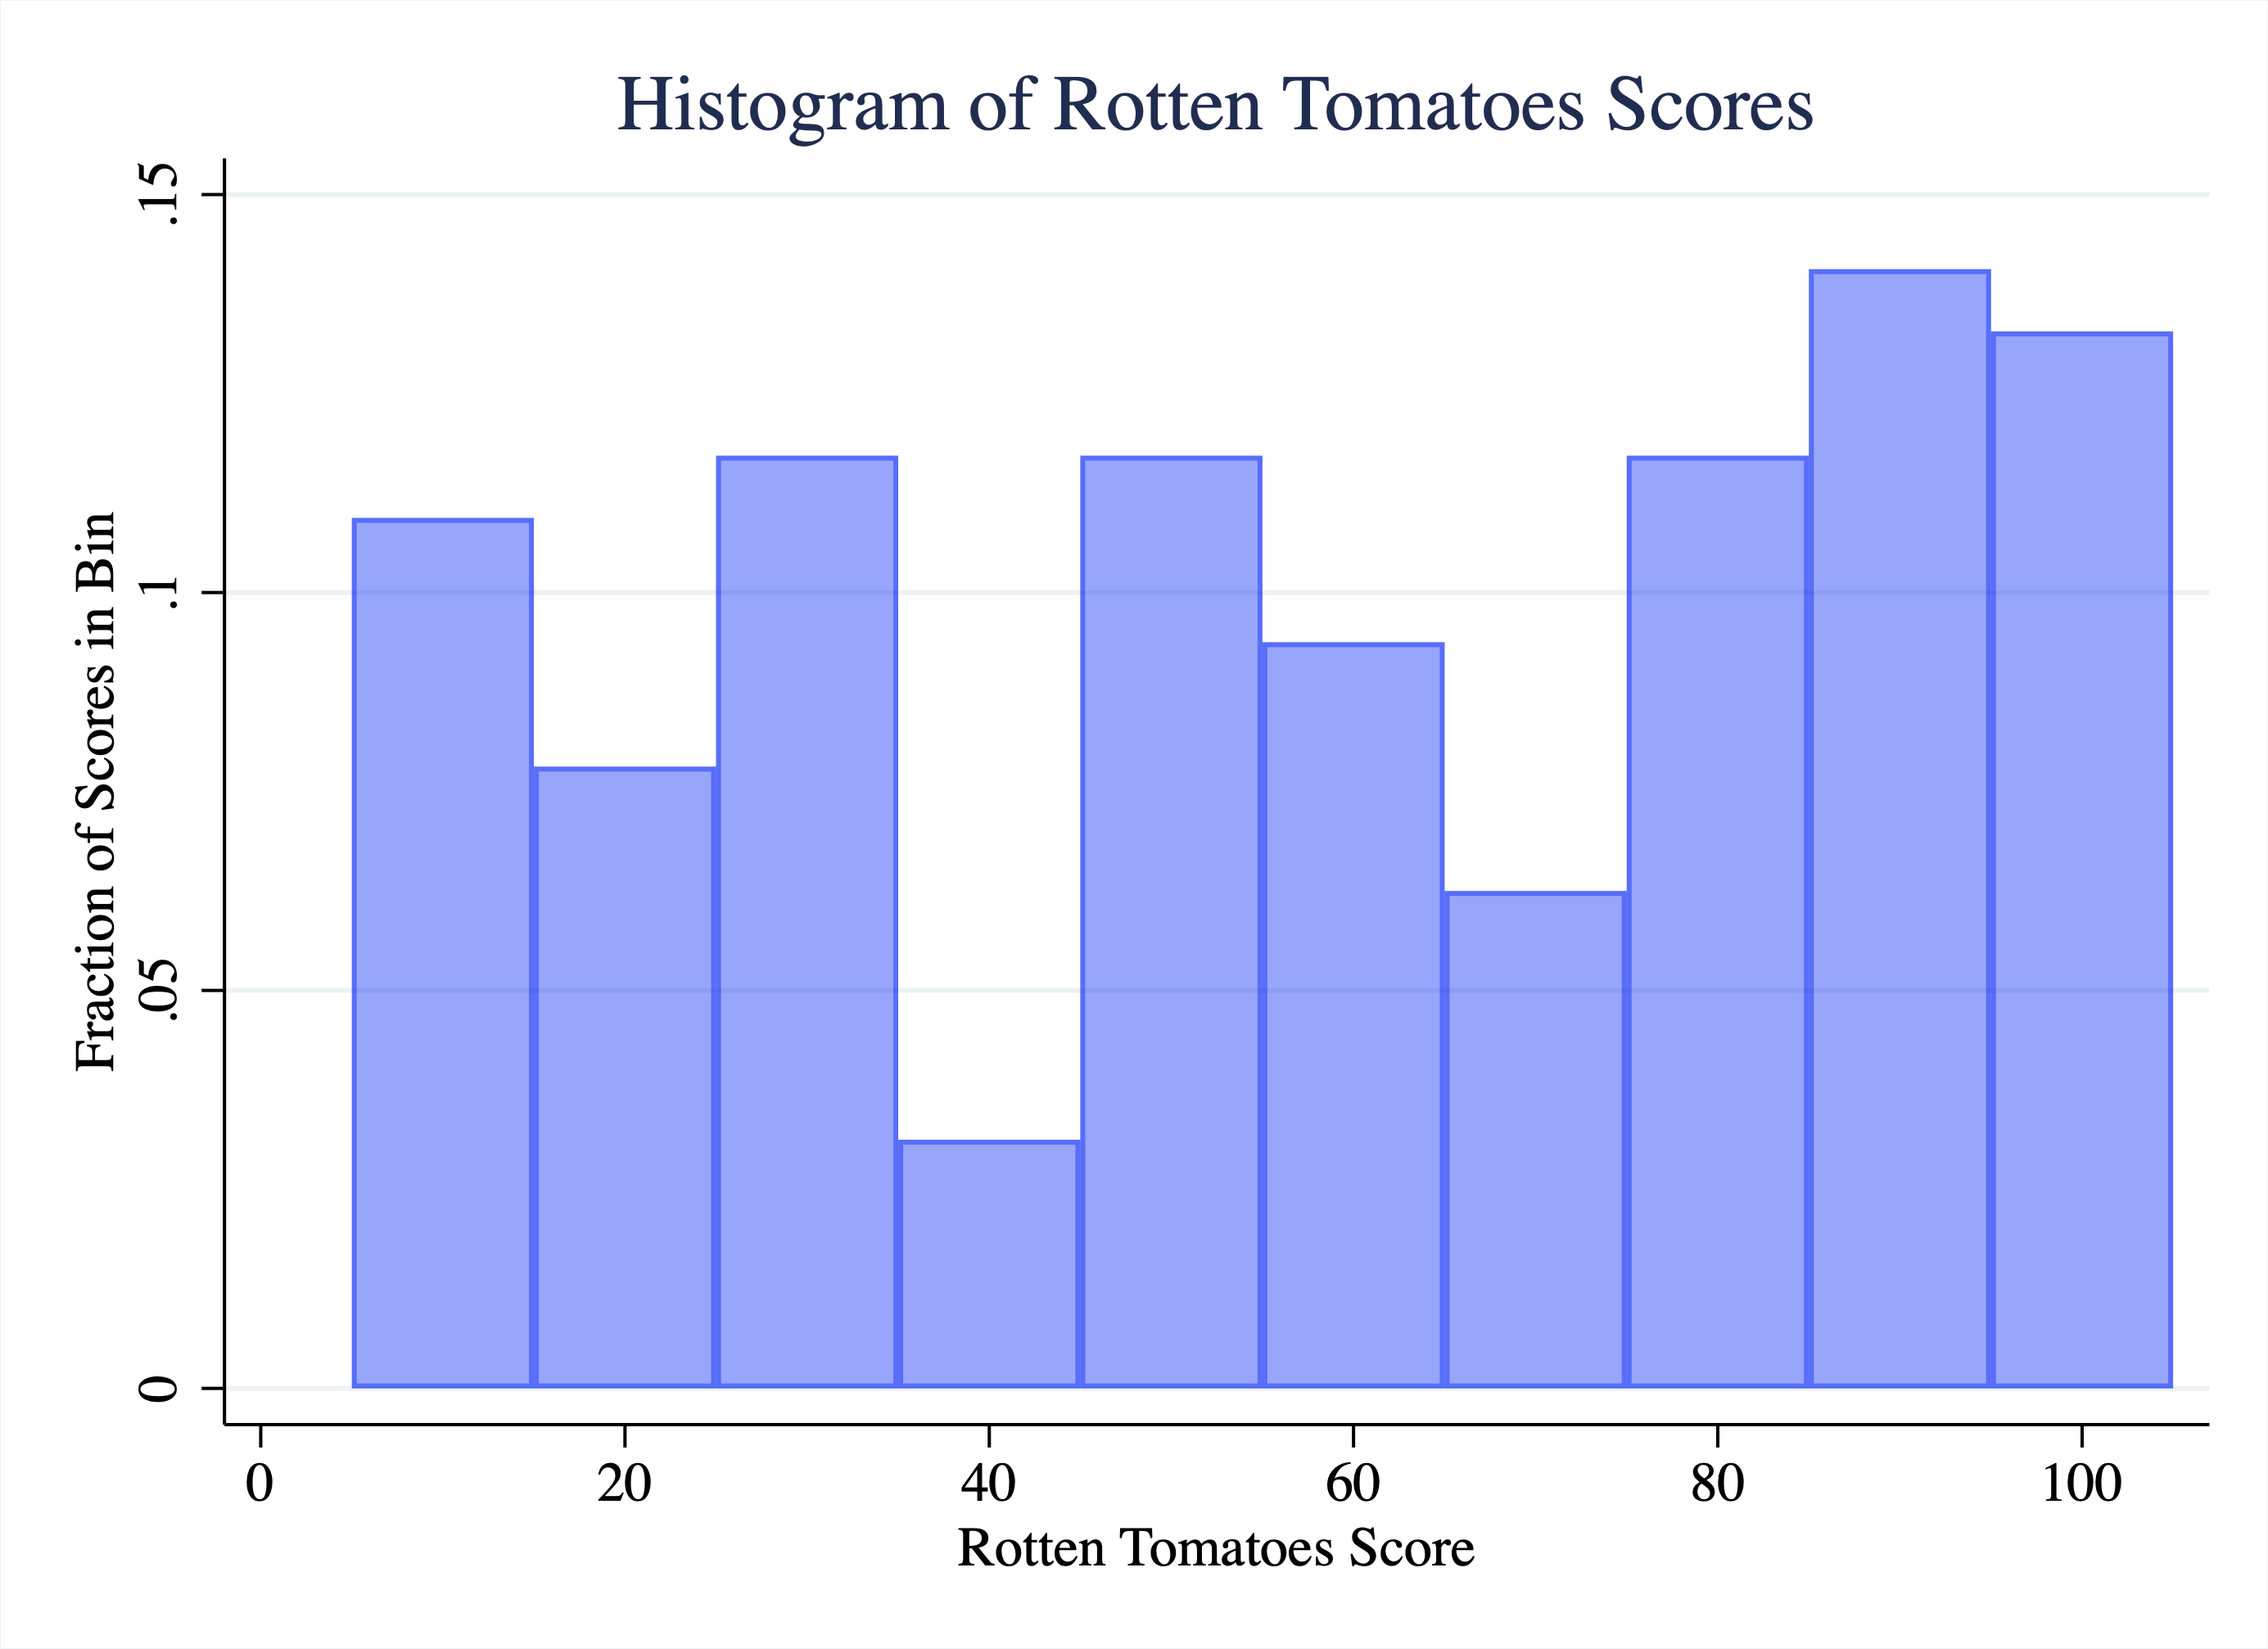
\includegraphics[width=0.75\linewidth]{images/02_movies1} 

}

\caption{Histogram of Rotten Tomatoes Scores for Movies Released in 2015}\label{fig:histmovies}
\end{figure}

So what do we learn from this figure? Some movies get very low scores, in the 5-10 range. How can we tell this? The first bin starts around 5 and ends around 15. The height of this bar is a little above 0.10. That means a bit more than 10 percent of all the movies got a score in the 5-15 range. As we move across the range of possible values, we actually find that the height of the bars is relatively stable. Therefore, we can describe this distribution as relatively uniform. That means across the range of movie scores, it does not seem like some scores are especially likely relative to others (for a perfectly uniform distribution the height of the bars would be identical across the entire range of the x-axis.)

In the next example, we are going to explore the distribution of Olympic athlete ages in Figure \ref{fig:athleteages}.

\begin{figure}

{\centering 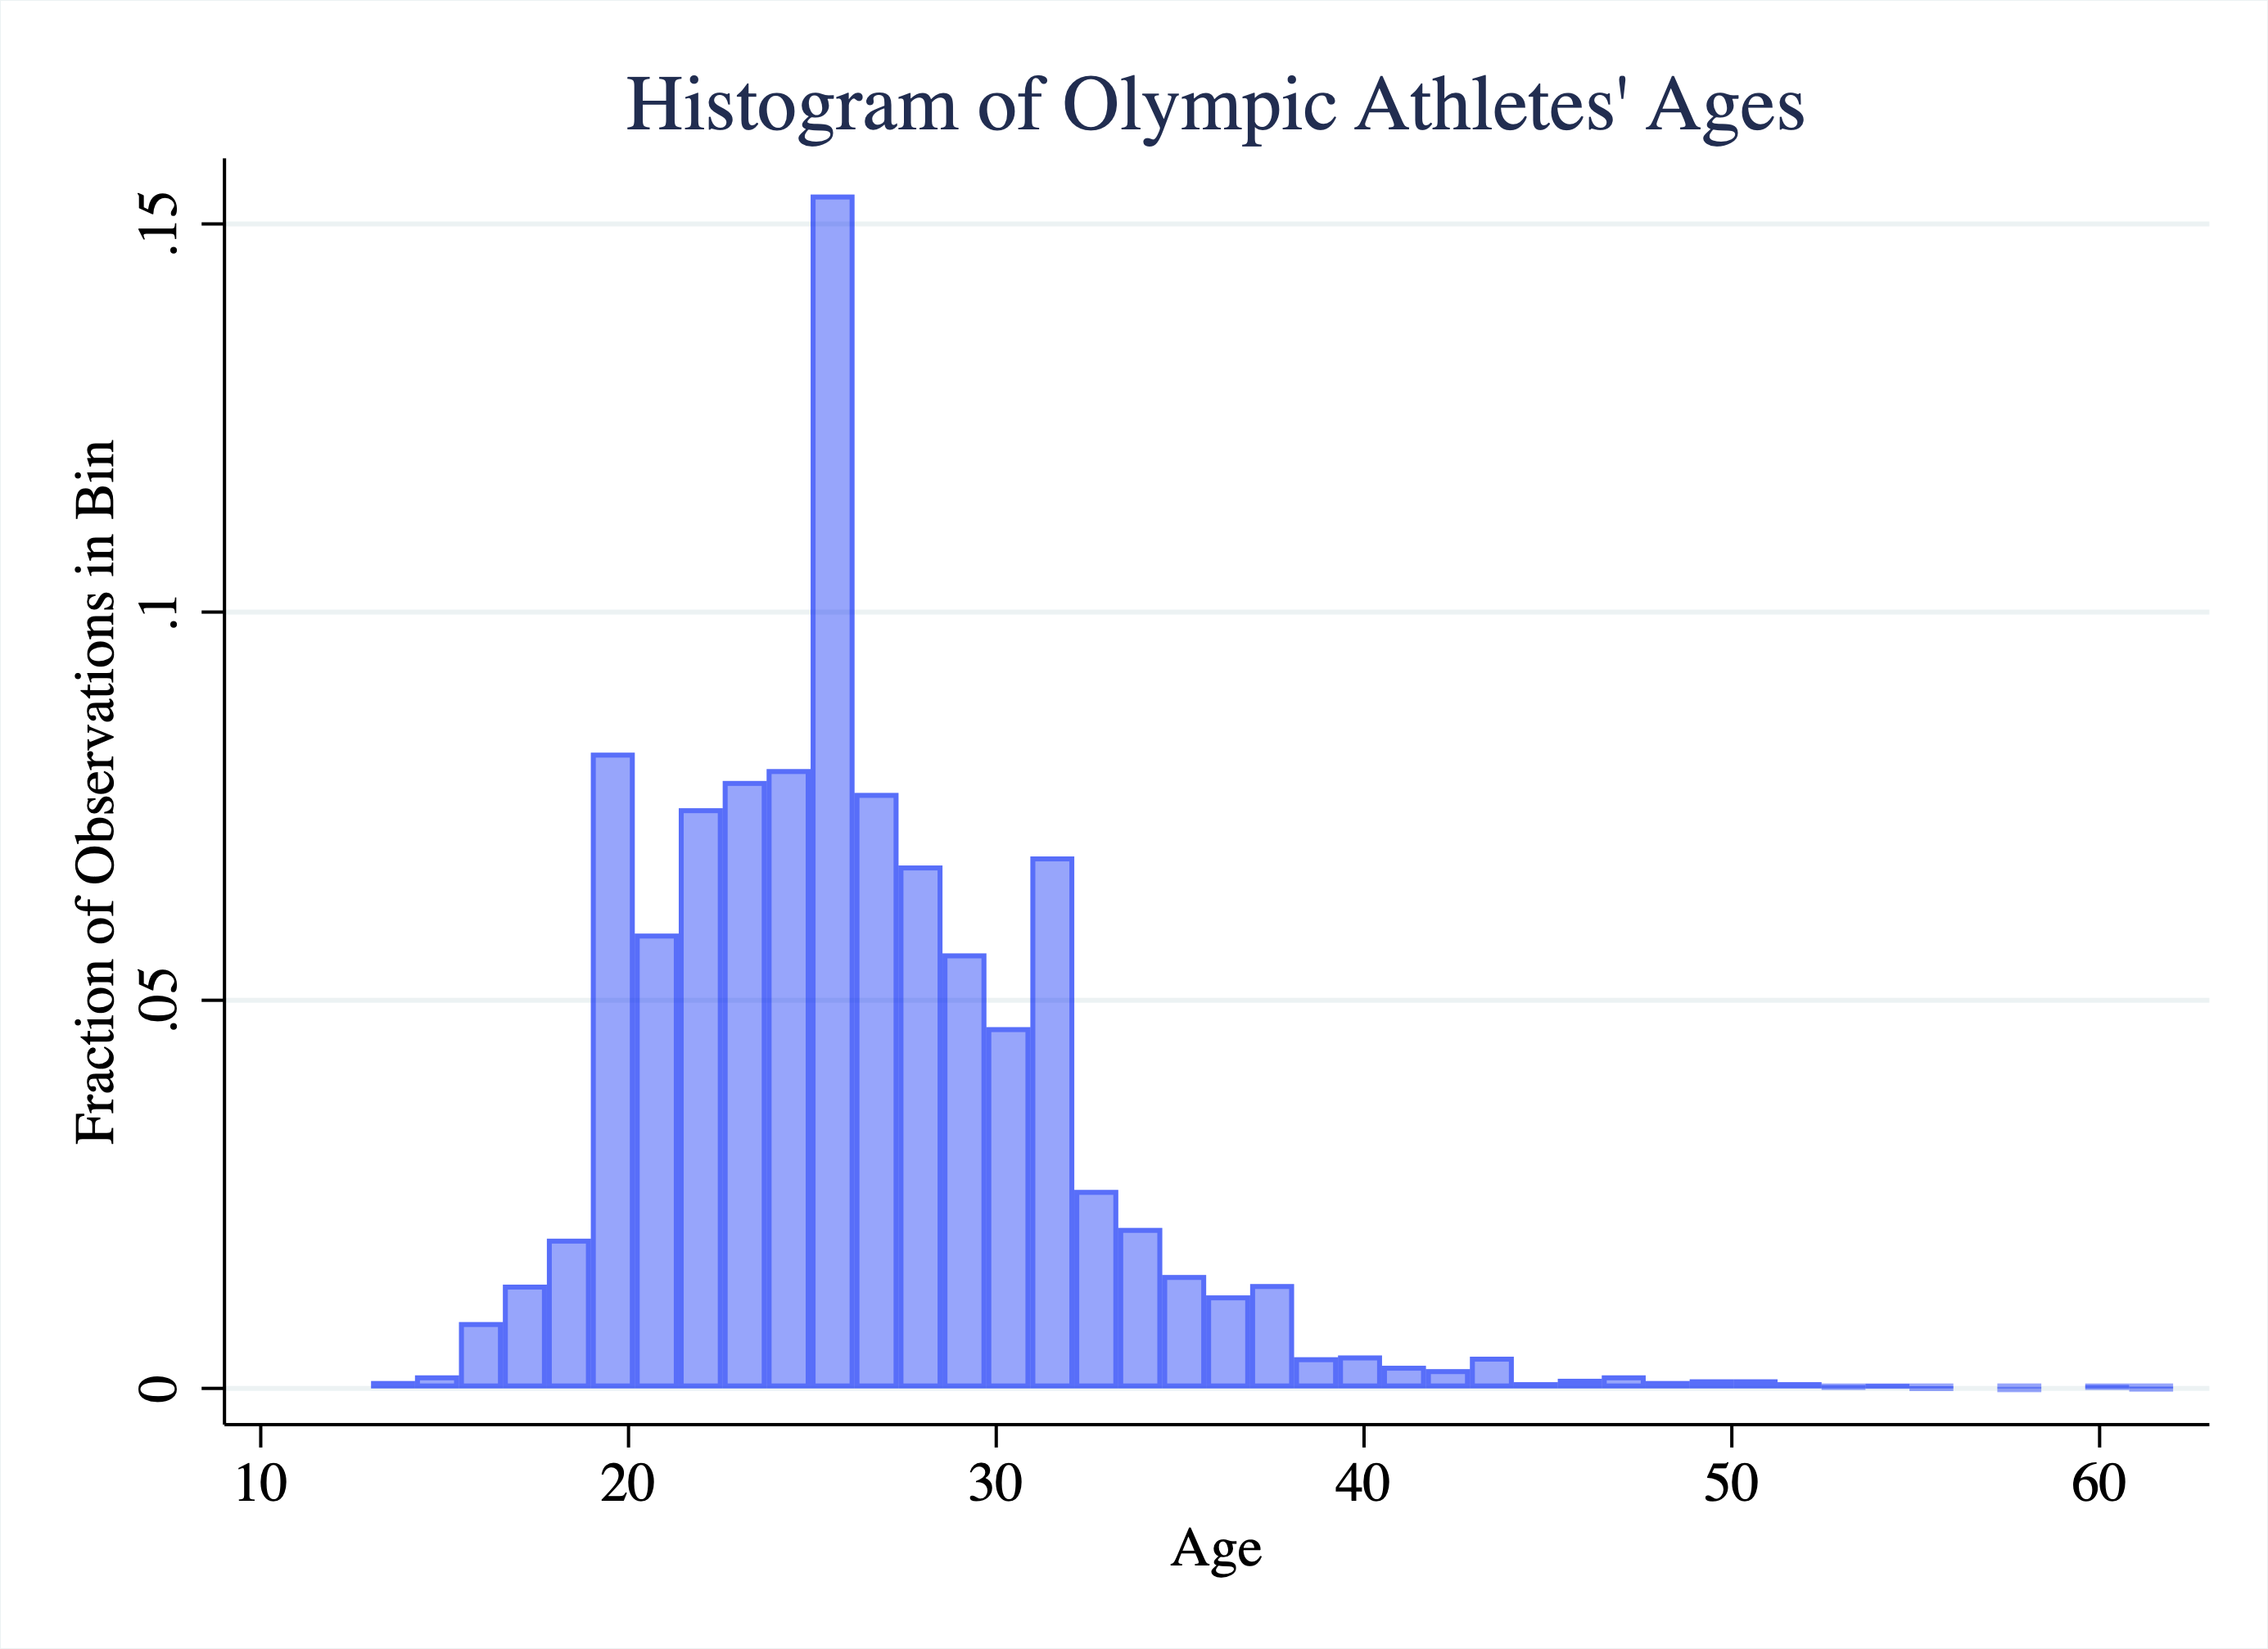
\includegraphics[width=0.75\linewidth]{images/02_athletes} 

}

\caption{Histogram of Olympic Athlete Ages}\label{fig:athleteages}
\end{figure}

So what do we learn from this histogram? Well, most Olympic athletes are between the ages of 19 and 32. Between these values the bars are consistently high, indicating a large fraction of the sample. At the lower end, there are some athletes under 19, but they are relatively less common. At the upper end, there are some athletes even above 40 years old, but these are clearly outliers. They are very far away from most of the data, which is in the 20s. We sometimes describe this feature of a distribution as a ``long-right tail''. Or we say the distribution is skewed right.

Finally, let's look at the distribution of calories for meals ordered at Chipotle in Figure \ref{fig:Chipotle}, which comes from an article in The Upshot.\citep{upshot}

\begin{figure}

{\centering 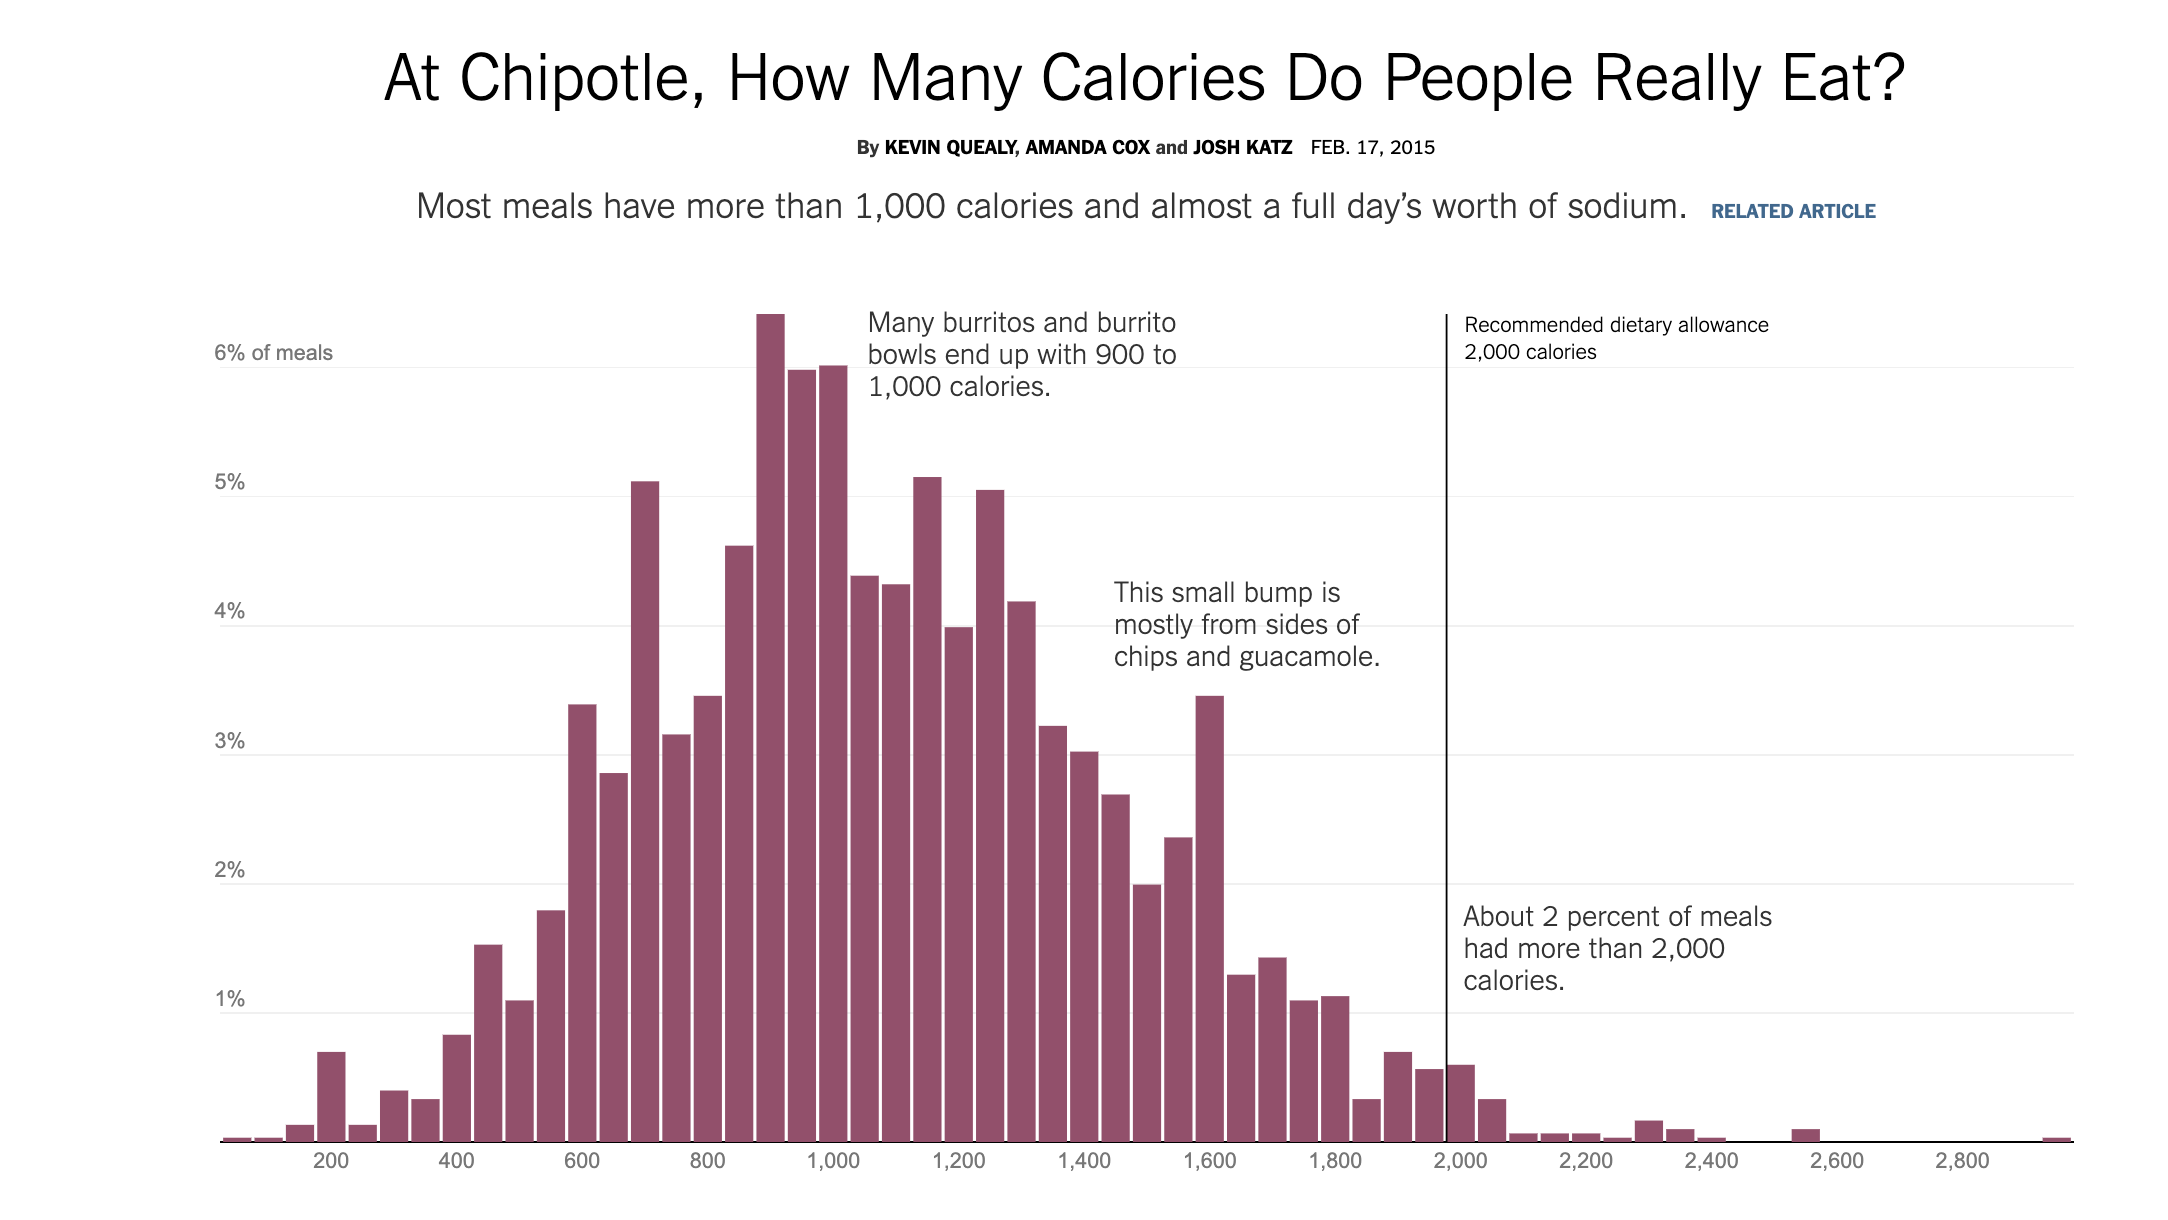
\includegraphics[width=1\linewidth]{images/02_chipotle} 

}

\caption{Histogram of Calories of Chipotle Meals}\label{fig:Chipotle}
\end{figure}

As we can see, most Chipotle meals are in the 1,000-calorie range. This is because many burritos and burrito bowls end up being around 1000 calories. However, if you order chips as well, that adds some calories to your meal, which is why we can see a bump in the histogram at around 1600 calories. At the upper end of the distribution, we see some meals have over 2,000 calories, more than the total amount of calories recommended in a day! Overall, about 2 percent of all meals have calorie counts this extreme.

\section{Histogram (Data)}\label{histogram-data}

In our empirical application, we want to understand the distribution of mobility rates across colleges. What are common values for the mobility rate? Are there outliers? To study this, we are going to create a histogram in Stata.

To begin, we need to learn about the \texttt{histogram} command, which is used to plot histograms in Stata. The simplest possible syntax is to simply type

\begin{Shaded}
\begin{Highlighting}[]
\KeywordTok{histogram}\NormalTok{ varname}
\end{Highlighting}
\end{Shaded}

Where \texttt{varname} is the name of whatever variable you would like to create a histogram for. In our example, we want to plot a histogram of \texttt{mobility\_rate}, so we will type:

\begin{Shaded}
\begin{Highlighting}[]
\KeywordTok{histogram}\NormalTok{ mobility\_rate}
\end{Highlighting}
\end{Shaded}

\begin{figure}

{\centering 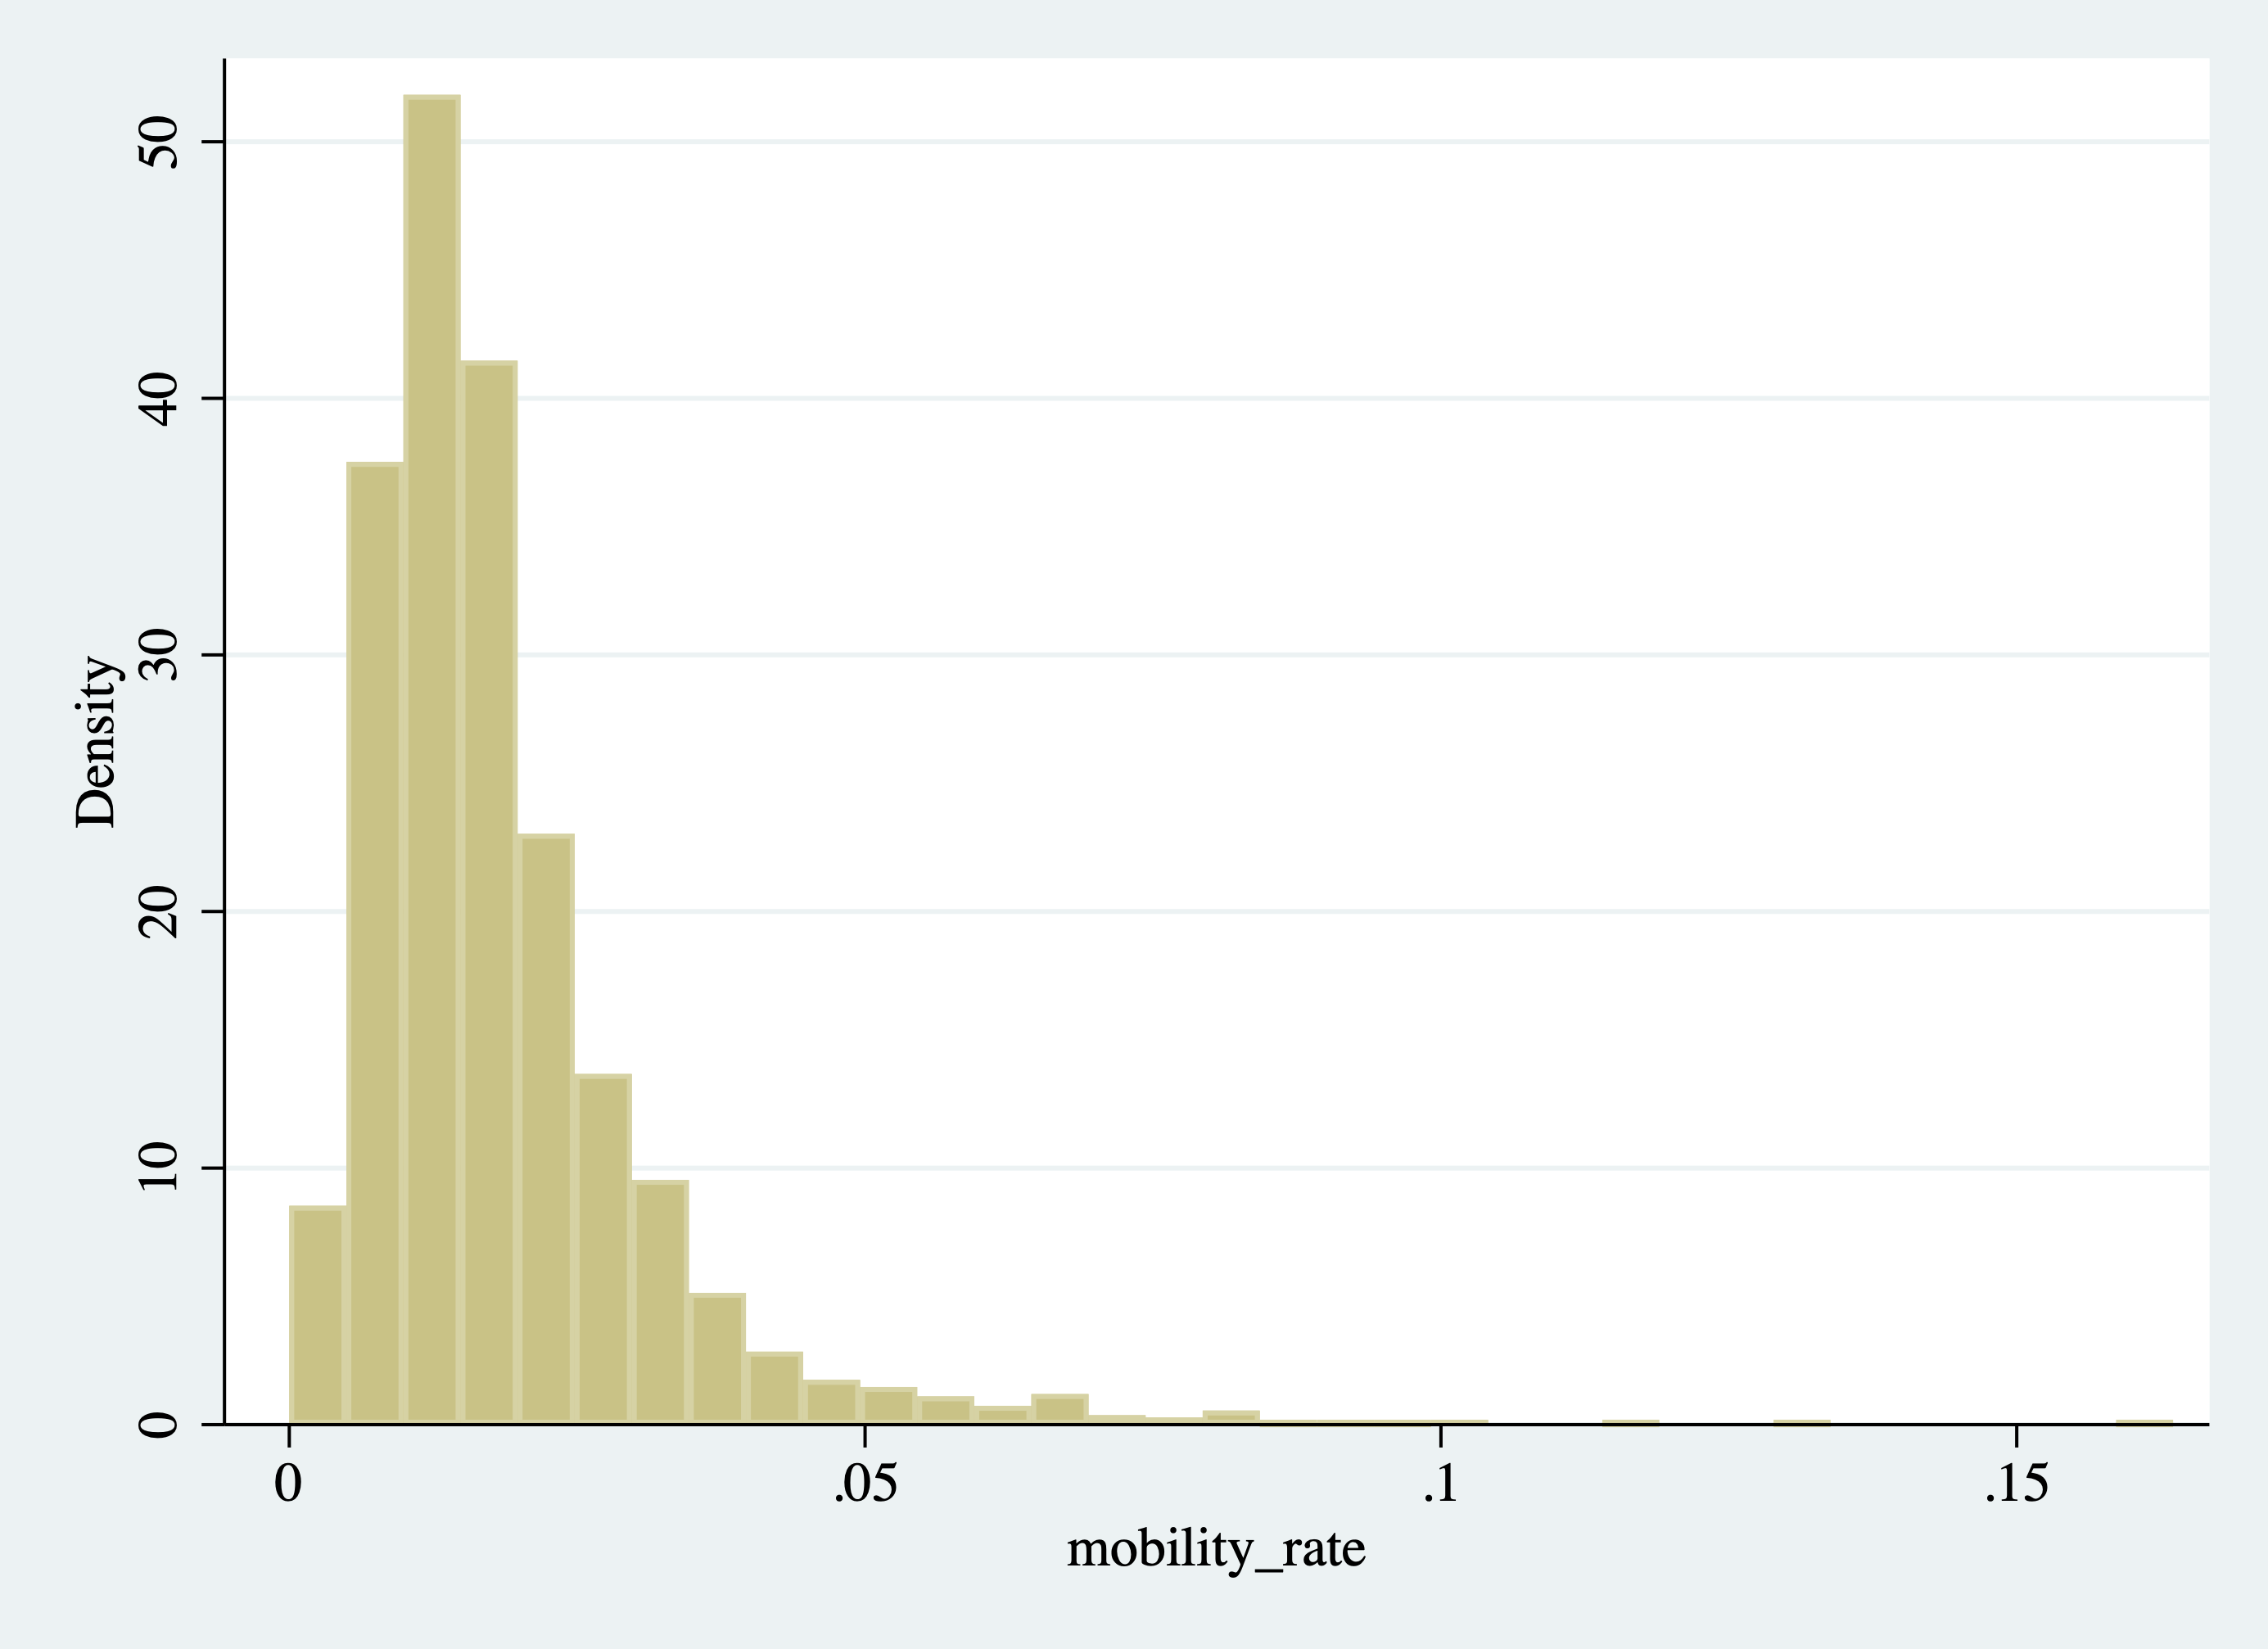
\includegraphics[width=0.85\linewidth]{images/02_hist1} 

}

\caption{Histogram of College Mobility Rates}\label{fig:mobilityhist1}
\end{figure}

You will notice that the vertical axis in Figure \ref{fig:mobilityhist1} is density. For our prior examples, we always had the vertical axis labeled as ``Fraction of Observations.'' It is not necessary to understand this for the class, but a density integrates to 1, which is why the vertical axis is sometimes rescaled in this way. For our purposes, it will be more intuitive to display the vertical axis as the fraction of observations. This will not change the appearance of the histogram in any way, just what is displayed on the vertical axis. To plot the fraction of observations instead of density, we can use an \textbf{option} of the histogram command.

In Stata, additional options are available for most commands. They give you a way to alter the command in some way. You can read through a list of options for a given command by opening the help file. The option we are looking for is the \texttt{frac} option, which changes the vertical axis to the fraction of observations instead of the density:

\begin{Shaded}
\begin{Highlighting}[]
\KeywordTok{histogram}\NormalTok{ mobility\_rate, frac}
\end{Highlighting}
\end{Shaded}

\begin{figure}

{\centering 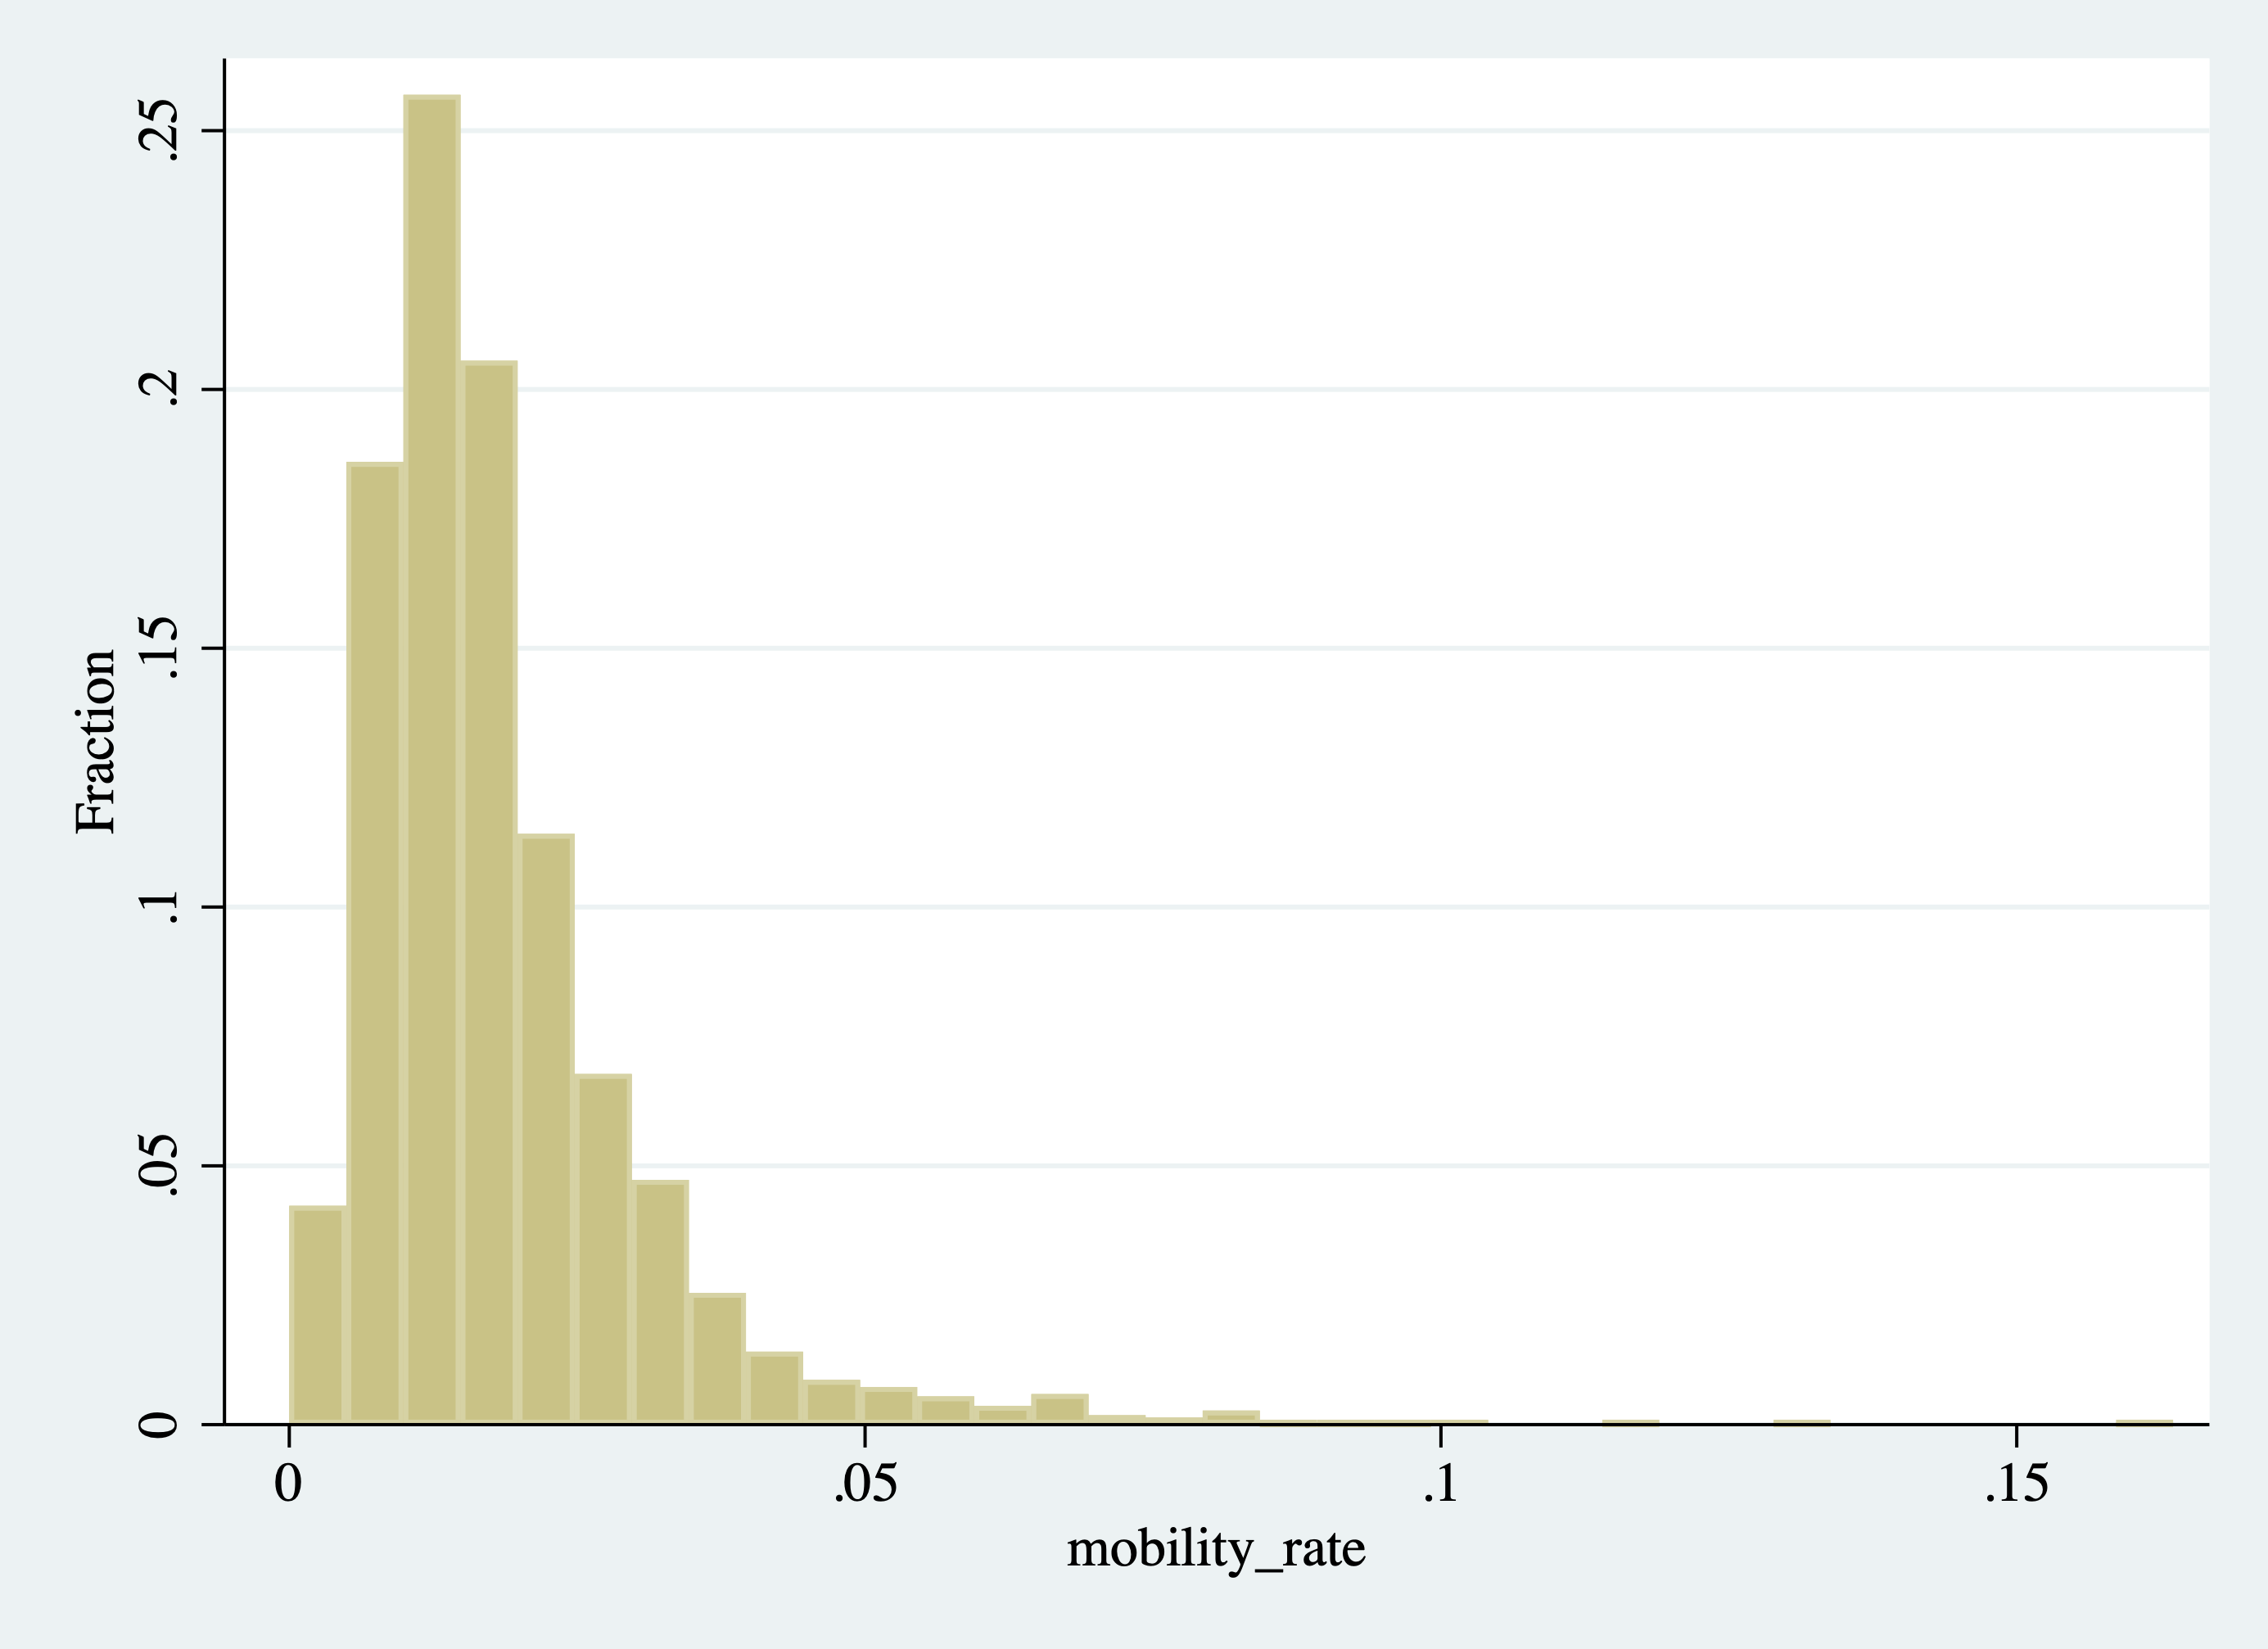
\includegraphics[width=0.85\linewidth]{images/02_hist2} 

}

\caption{Histogram of College Mobility Rates (Changing the Vertical Axis)}\label{fig:mobilityhist2}
\end{figure}

Now that we have our histogram, let's start interpreting it. First, where is most of the ``mass'' of the histogram (i.e.~where are the bars the highest)? This will be where most colleges fall in terms of mobility rates. Well, it looks like there is a spike near 0.02. For example, the highest bar in this range reaches 0.25, indicating 25 percent of all colleges fall in that interval. What does a value of 0.02 represent? A college with a mobility rate of 0.02 has 2 percent of its students coming from low-income backgrounds and achieving high income.

Two percent seems like a low number, but there are colleges with even lower rates of mobility. For example, the first interval starts at roughly zero. The height of this bar is around 0.04, indicating about 4 percent of schools have mobility rates near zero. Again, this could be due to either (1) not accepting students from low-income backgrounds (access) or (2) having graduates that do not earn enough to be categorized as high income (success).

On the other end of the distribution, we can see some outlier schools have very high mobility rates relative to others. Although it is difficult to see in the graph, there are a few schools with mobility rates above 0.10, indicating over 10 percent of the students in the school come from low-income backgrounds and achieve high income later in life.

Overall this is an example of a distribution with a long-right tail. Most schools cluster in the 0.01 to 0.03 range, but there are some outliers at the upper end of the mobility distribution.

Sometimes it is helpful to tweak your graphs. In some cases, you may not like the default settings, and so generally, you will be able to change them. For example, maybe we do not like how many bins were created. We can directly control the number of bins by specifying the \texttt{bin()} option. For example, in Figure \ref{fig:mobilityhist6} we create a histogram with 20 bins.

\begin{Shaded}
\begin{Highlighting}[]
\KeywordTok{histogram}\NormalTok{ mobility\_rate, frac }\BaseNTok{bin}\NormalTok{(20)}
\end{Highlighting}
\end{Shaded}

\begin{figure}

{\centering 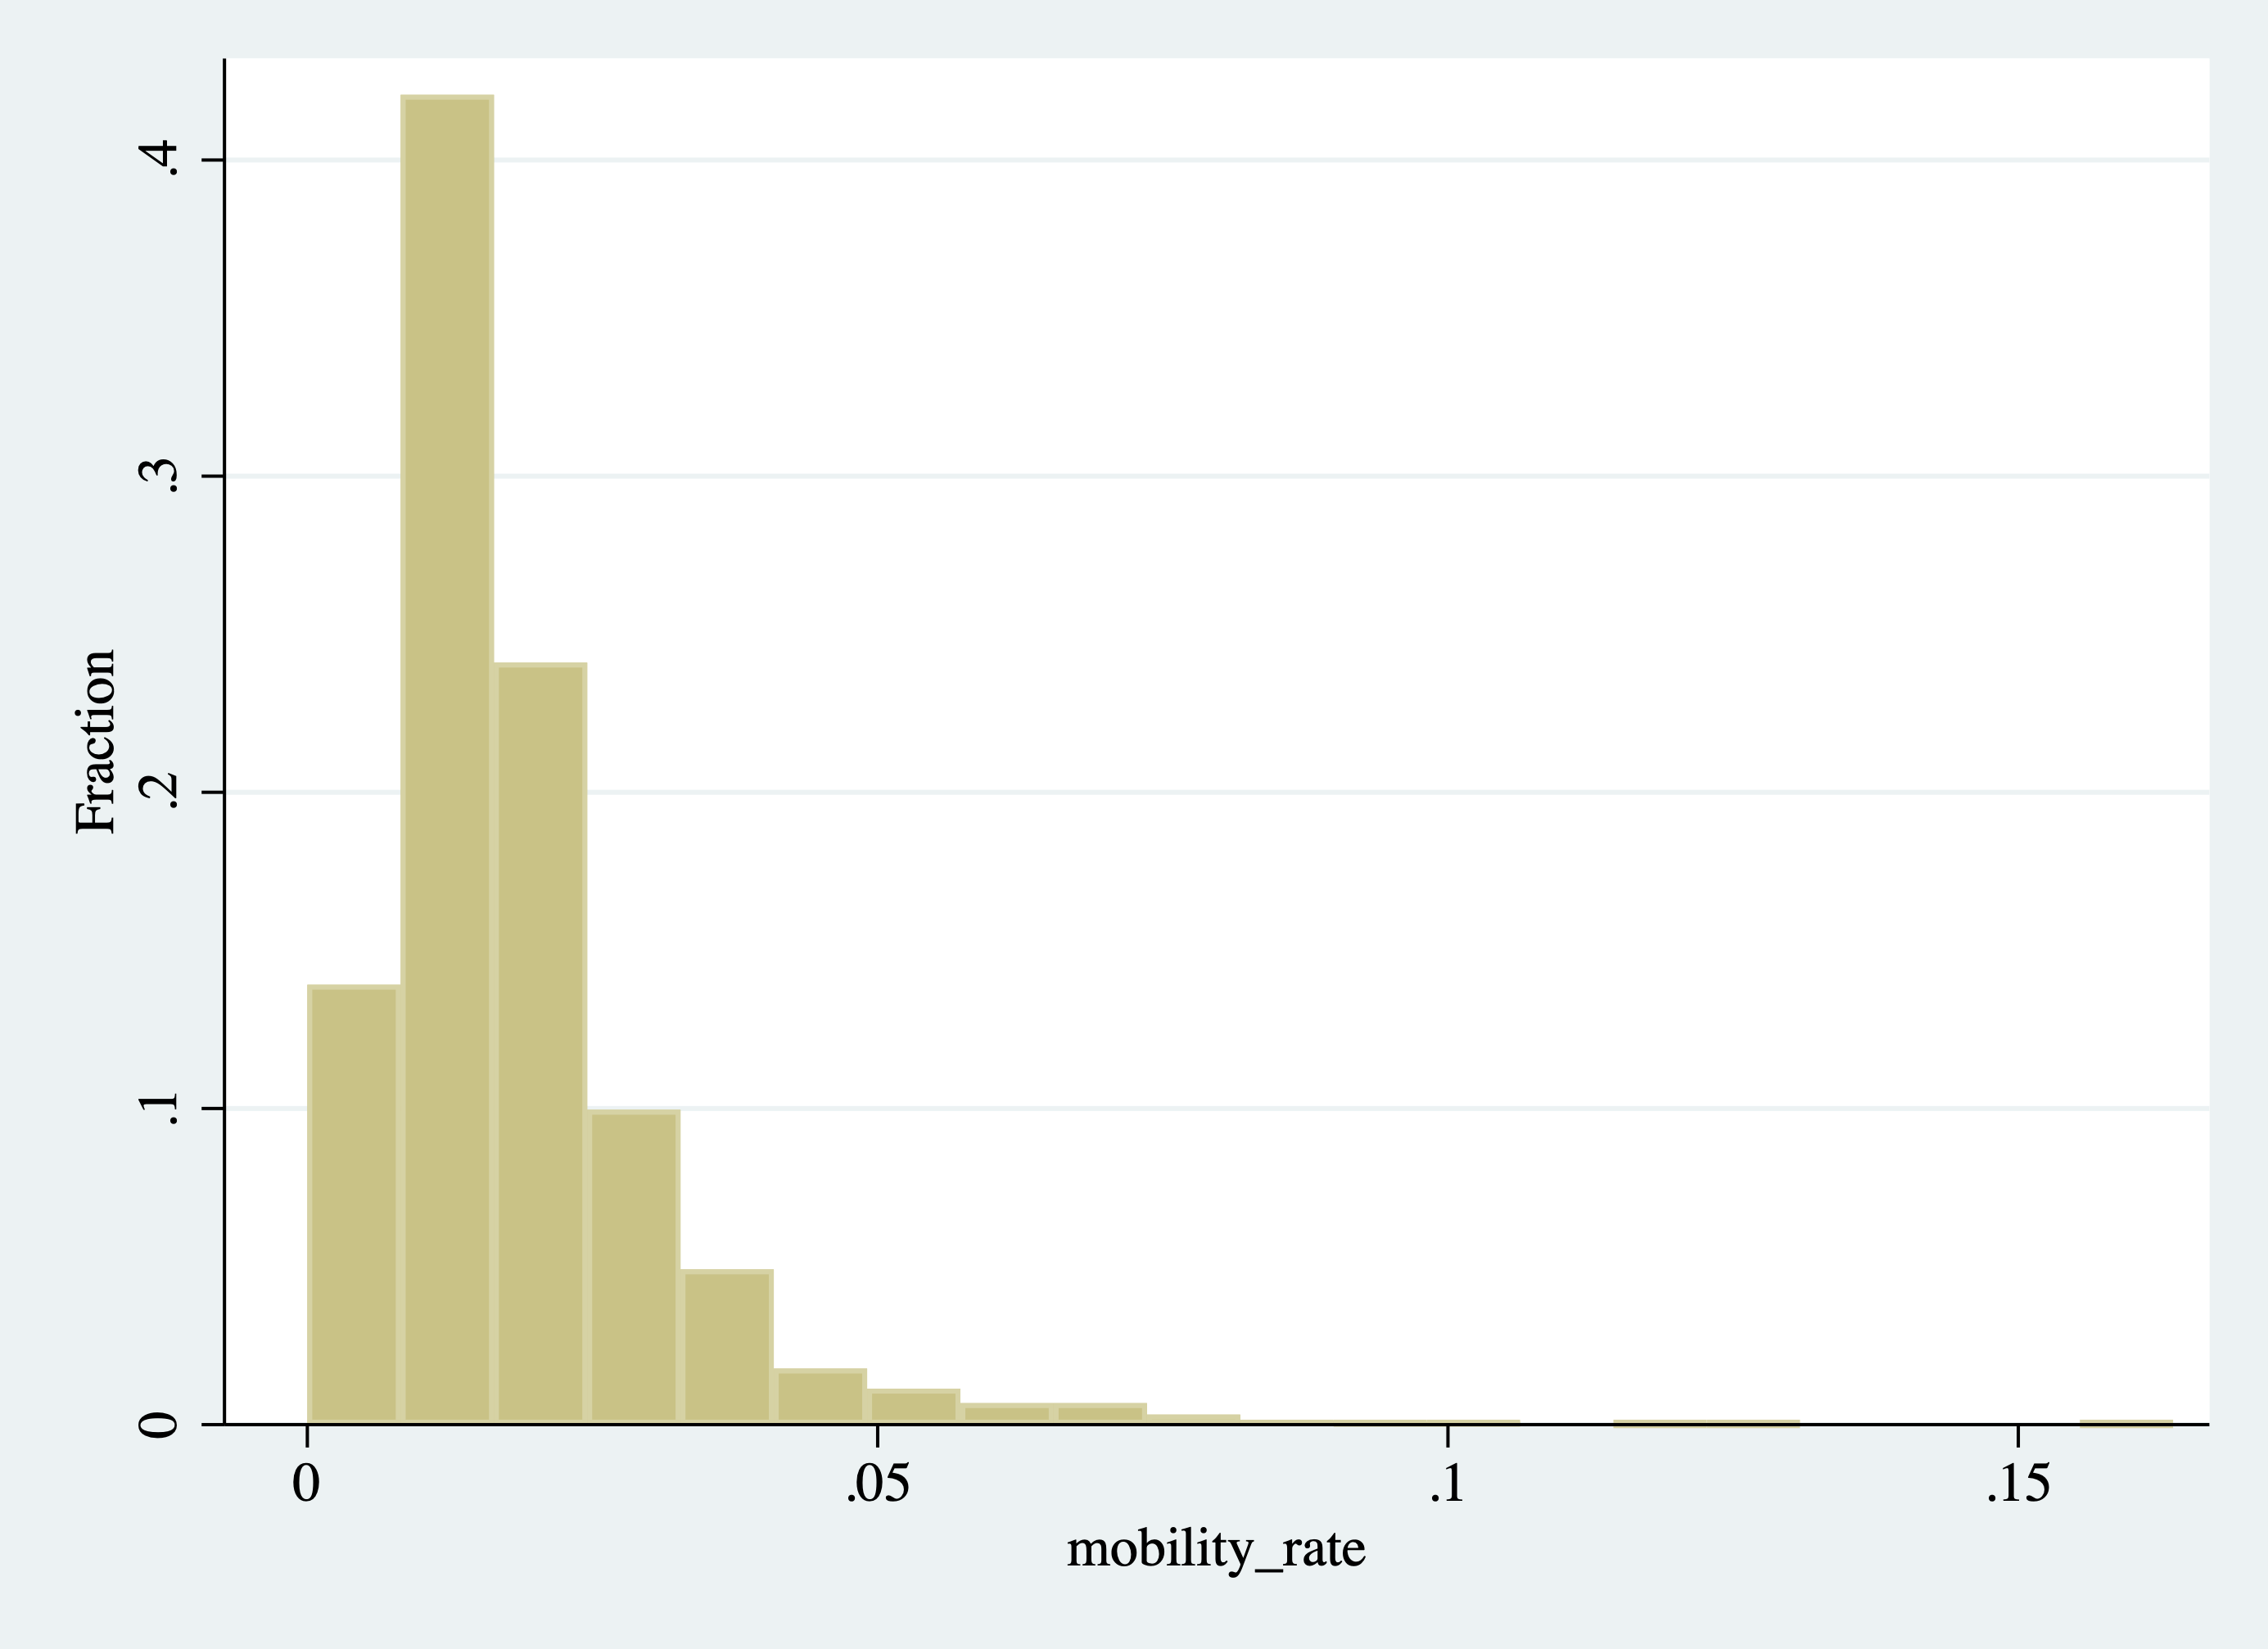
\includegraphics[width=0.85\linewidth]{images/02_hist6} 

}

\caption{Histogram of College Mobility Rates (Changing the Number of Bins)}\label{fig:mobilityhist6}
\end{figure}

Because there were more than 20 bins in our original histogram, the width of each bin is larger now (some of the bin heights at the upper end of the distribution are very small and difficult to see in the figure).

Instead of directly controlling how many bins, we can also control the width of the bins. In our test score example, we chose bins of width 10, but we could have chosen bins of width 5 instead. The choice of 10 was arbitrary. In some cases, you may want to change the width of the bins. To change the width of the bin we can specify the \texttt{width()} option, as we do below.

\begin{Shaded}
\begin{Highlighting}[]
\KeywordTok{histogram}\NormalTok{ mobility\_rate, frac }\KeywordTok{width}\NormalTok{(0.01)}
\end{Highlighting}
\end{Shaded}

\begin{figure}

{\centering 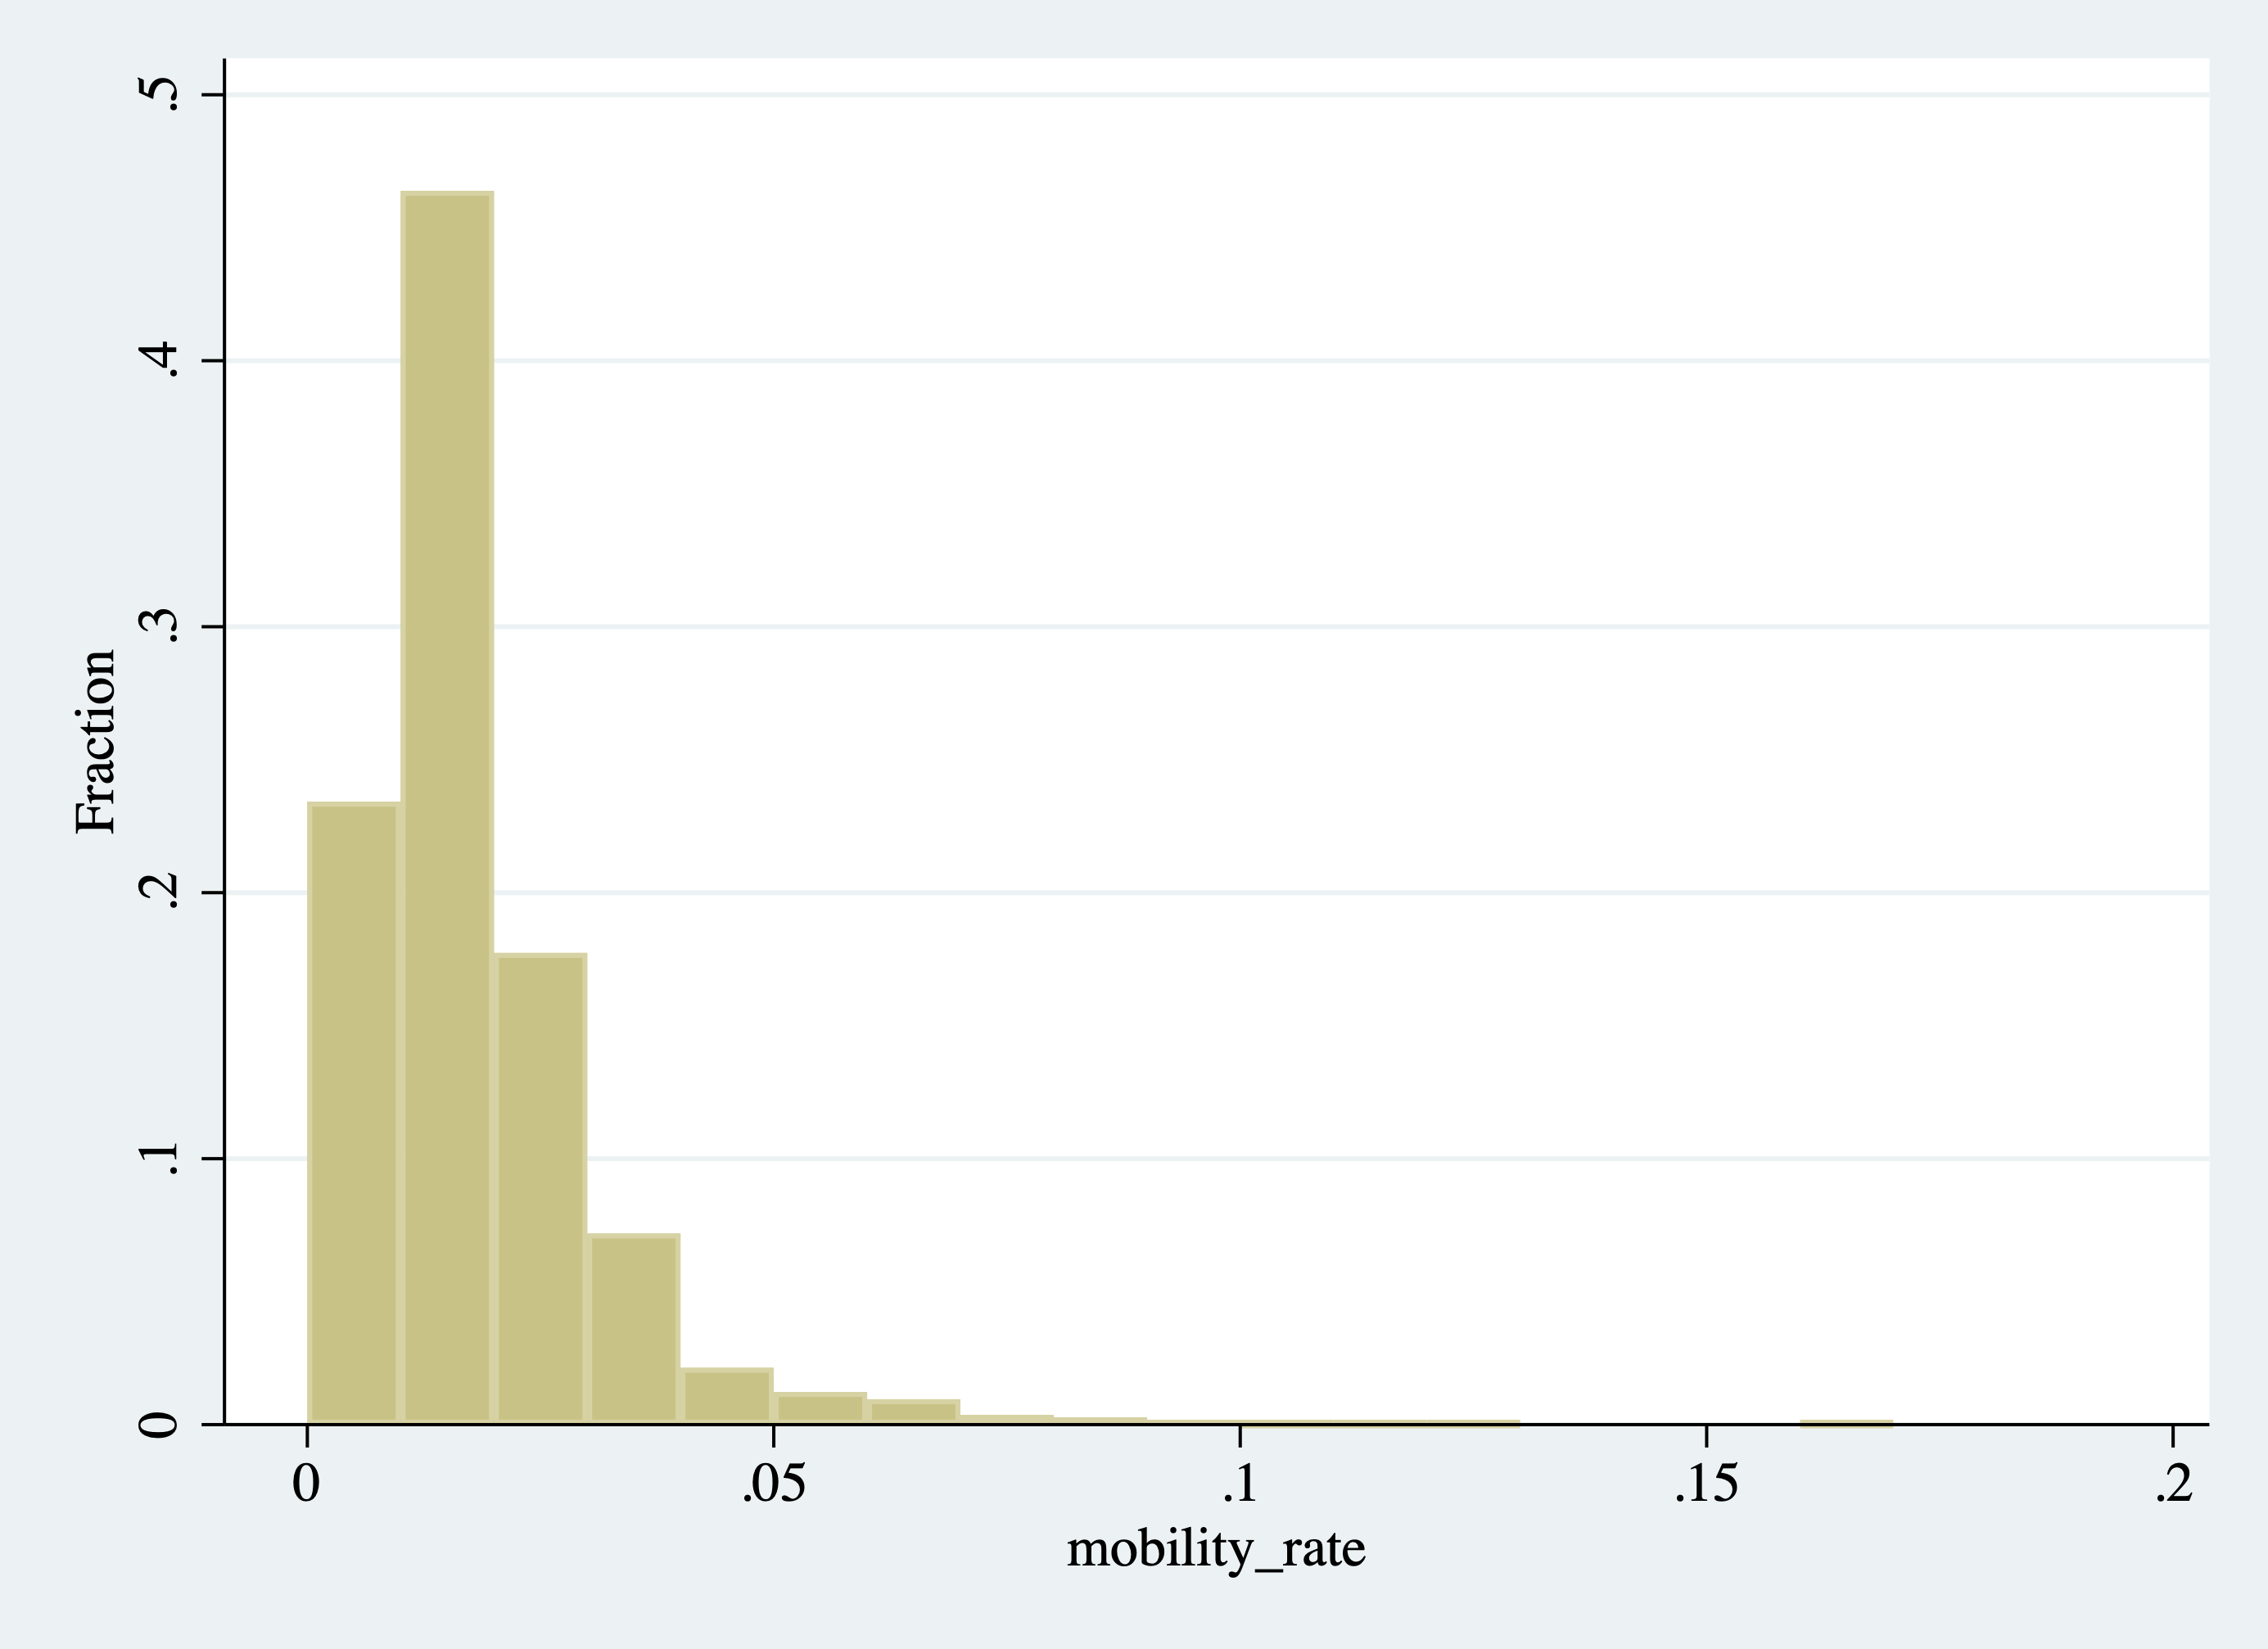
\includegraphics[width=0.85\linewidth]{images/02_hist7} 

}

\caption{Histogram of College Mobility Rates (Changing the Width of the Bins)}\label{fig:mobilityhist7}
\end{figure}

In Figure \ref{fig:mobilityhist7}, the interval of each bin is 0.01. Given the range of the data, this creates about 20 equal-sized bins, which is why this figure looks similar to the figure we created when we specified 20 bins.

\section{Histogram (Aesthetics)}\label{histogram-aesthetics}

Although we have created a histogram, it still leaves a lot to be desired. For our figures to be effective, they need to be clearly labeled and titled. To make them more visually appealing, it is also helpful to change colors and add additional elements.

To change the color of the bars in our graph, we can specify the \texttt{color()} option. What I find to be effective in histograms is to also make the bars slightly translucent. This allows for plotting multiple histograms on the same figure, while still being able to distinguish the different variables. In the code below, we are going to change the color of our bars to blue, but then also make the bars transparent. We will do this by specifying \texttt{color(blue\%40)} as one of the command options. The \texttt{\%40} will control how translucent the bars appear. You can specify any number between zero and 100 here.

\begin{Shaded}
\begin{Highlighting}[]
\KeywordTok{histogram}\NormalTok{ mobility\_rate, frac }\KeywordTok{color}\NormalTok{(}\BaseNTok{blue}\NormalTok{\%40)}
\end{Highlighting}
\end{Shaded}

\begin{figure}

{\centering 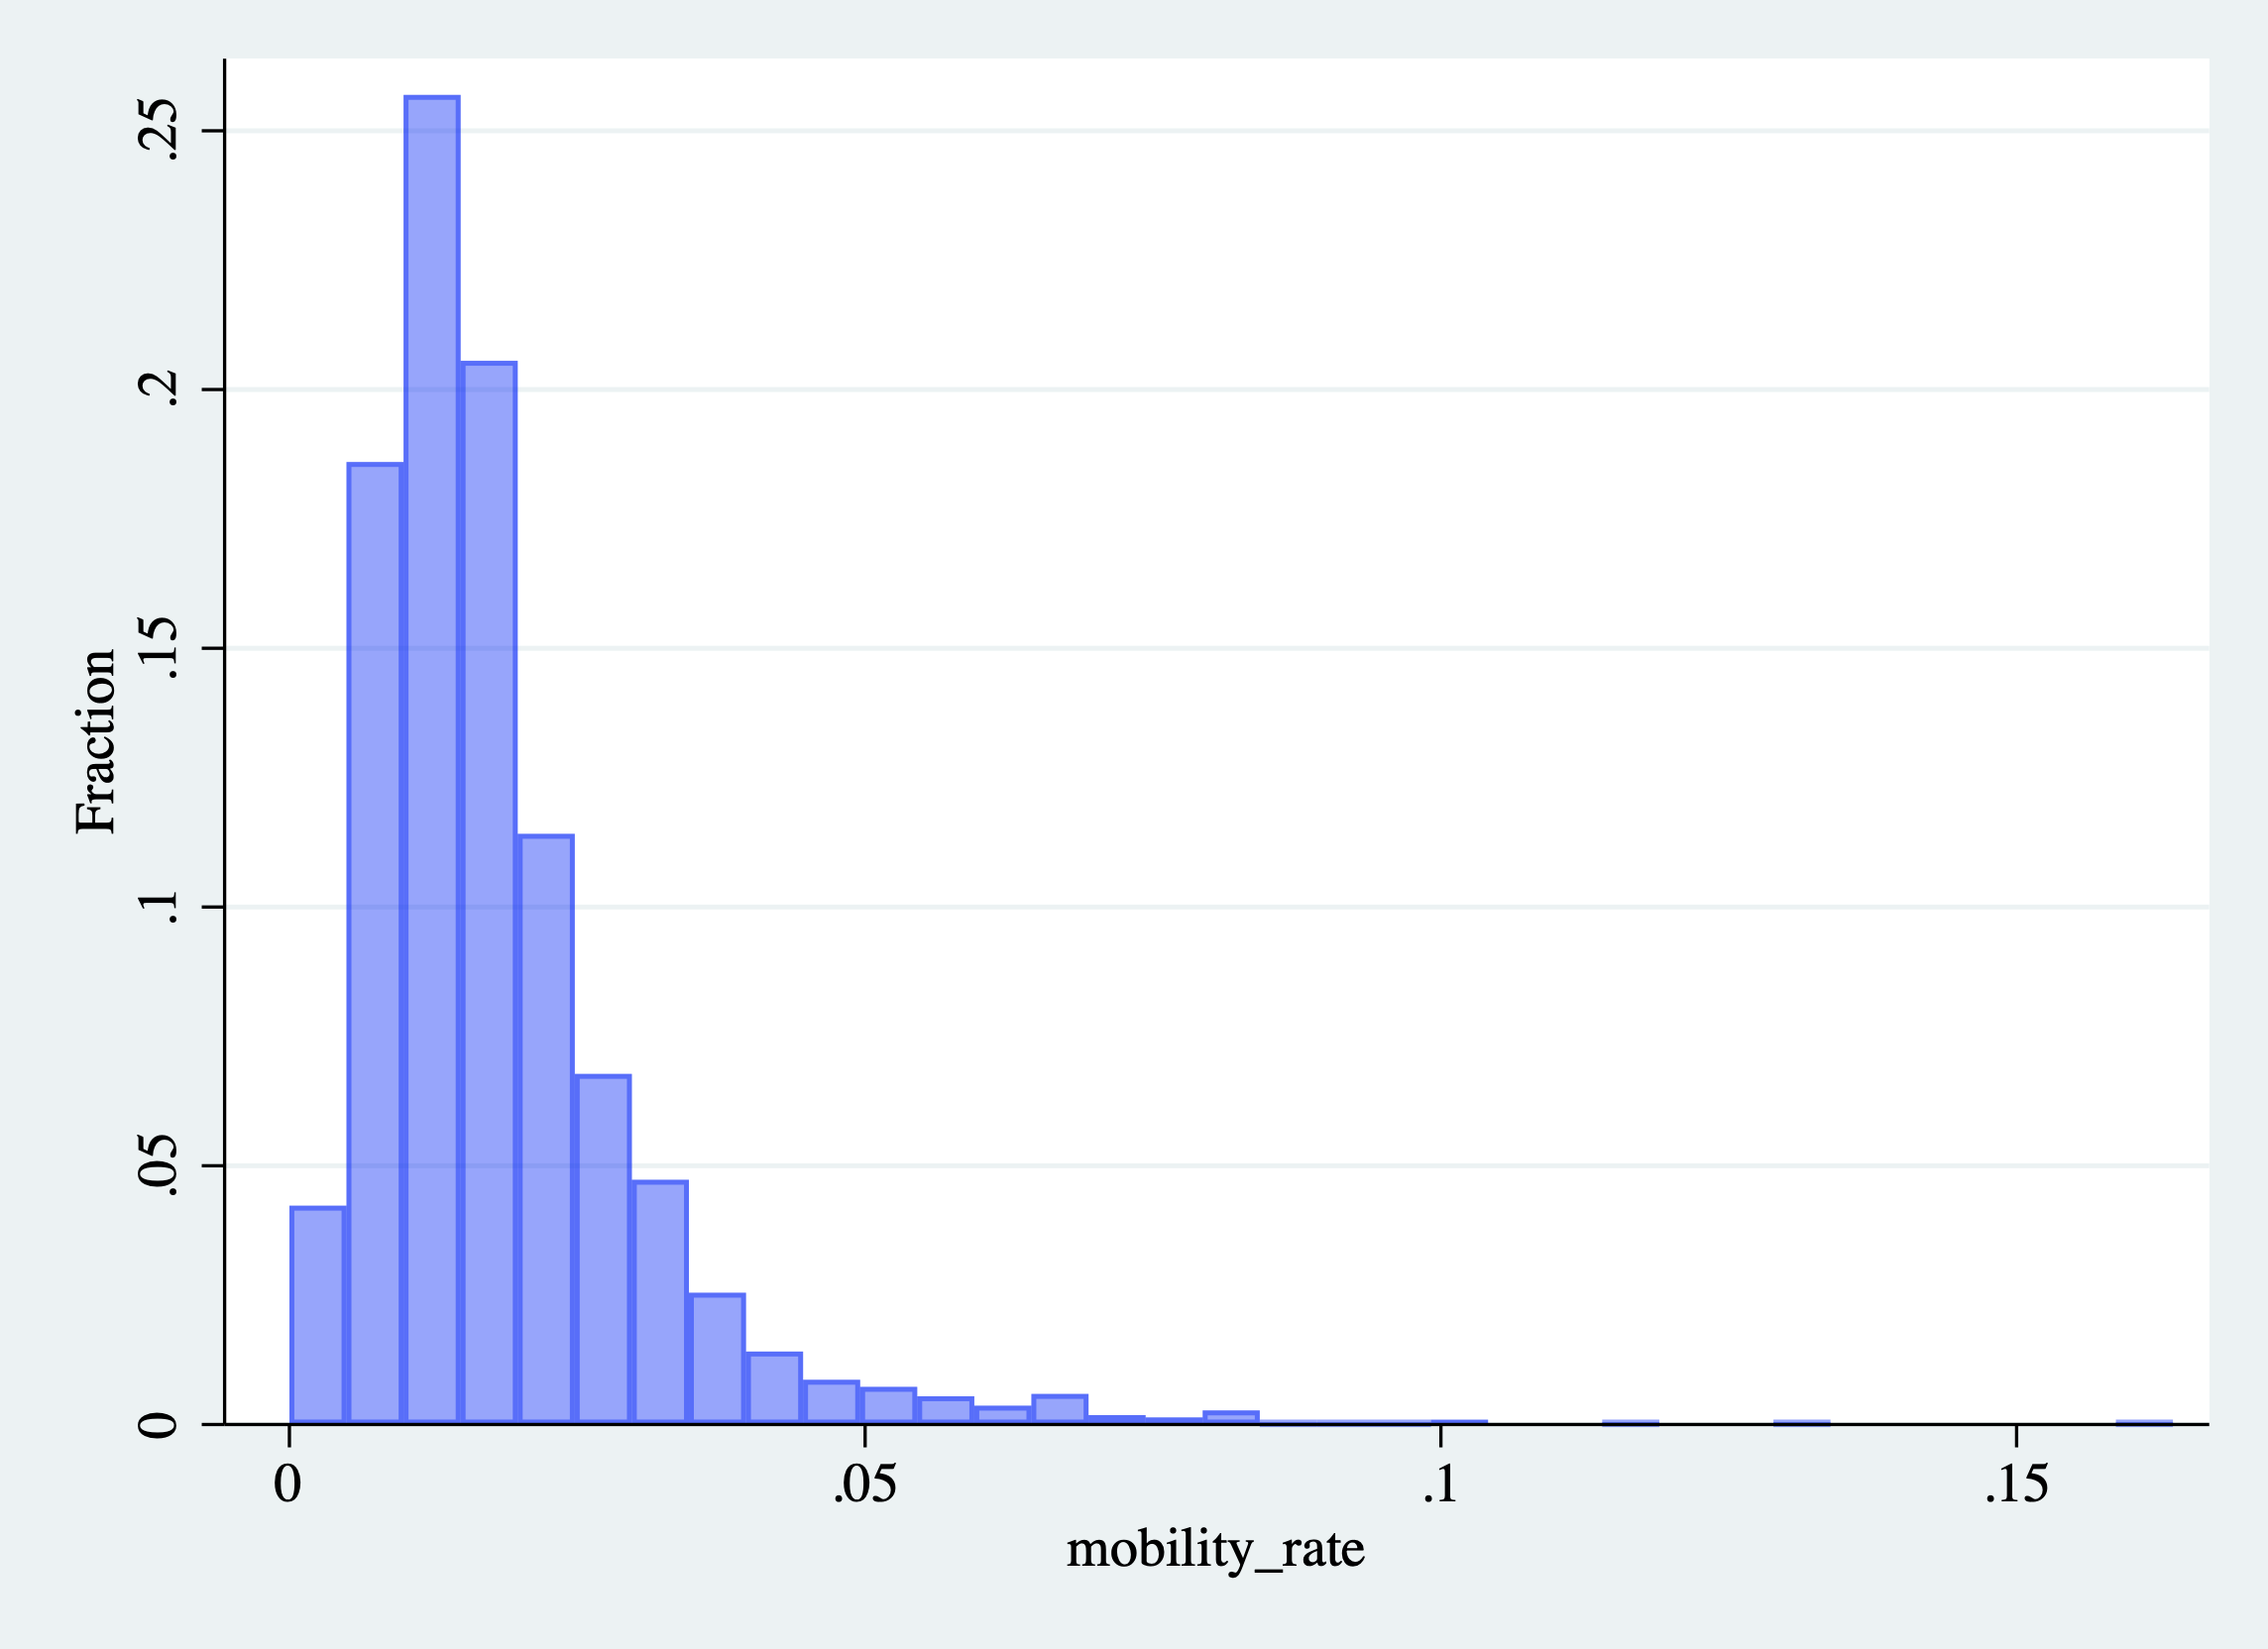
\includegraphics[width=0.85\linewidth]{images/02_histae2} 

}

\caption{Histogram of College Mobility Rates (Changing the Color of the Bars)}\label{fig:histae2}
\end{figure}

Next, let's add a title to our figure. It is always important to include a title that describes what the figure is presenting. We can do this by specifying the \texttt{title()} option:

\begin{Shaded}
\begin{Highlighting}[]
\KeywordTok{histogram}\NormalTok{ mobility\_rate, frac }\KeywordTok{color}\NormalTok{(}\BaseNTok{blue}\NormalTok{\%40) }\CommentTok{///}
  \BaseNTok{title}\NormalTok{(}\StringTok{"Histogram of Mobility Rates Across U.S. Colleges"}\NormalTok{)}
\end{Highlighting}
\end{Shaded}

\begin{figure}

{\centering 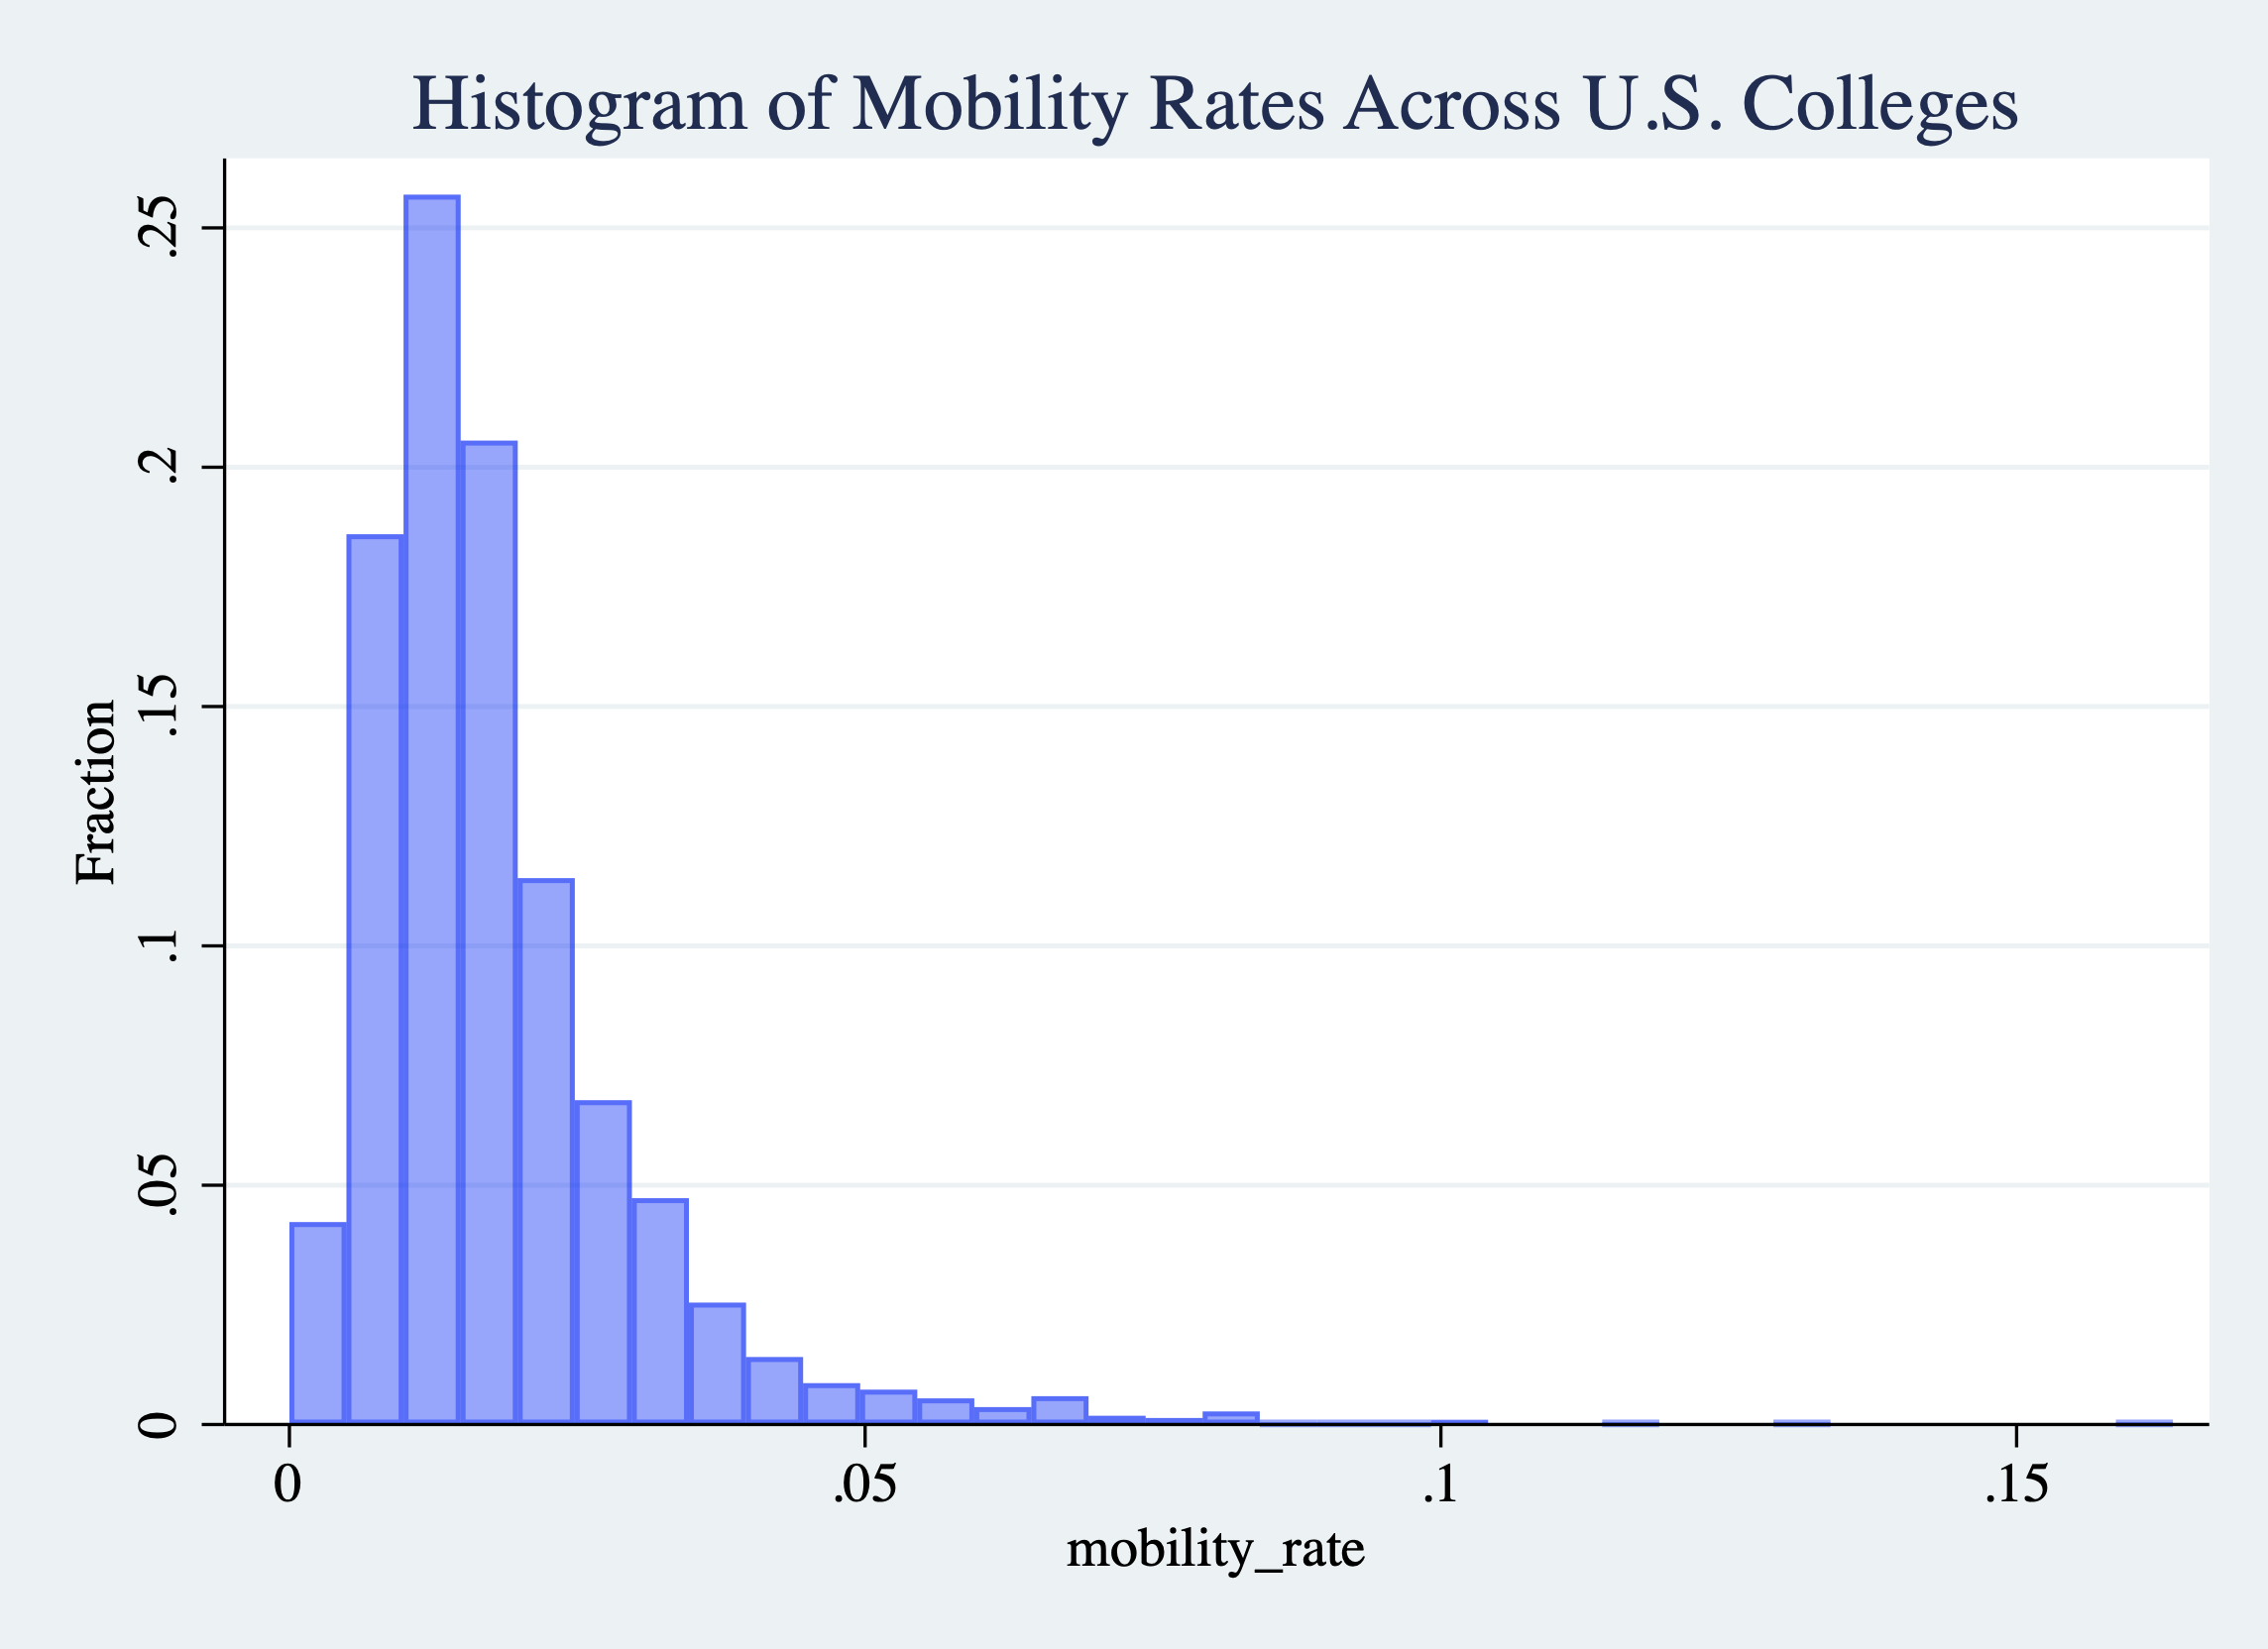
\includegraphics[width=0.85\linewidth]{images/02_histae3} 

}

\caption{Histogram of College Mobility Rates (Adding a Title)}\label{fig:histae3}
\end{figure}

You will notice the three \texttt{///} at the end of the first line of code. Sometimes it is easier to read code if we separate the various elements into different lines. However, in Stata, if you press enter and continue your code on the next line, then Stata will not interpret the two lines as connected. In other words, if we did not include the \texttt{///} it will interpret the second part \texttt{title("Histogram\ of\ Mobility\ Rates\ Across\ U.S.\ Colleges")} as a new block of code. But \texttt{title} is not a command in Stata, it is an option of graphical commands. Therefore, it needs to follow some type of graphing command. By adding the \texttt{///} we are telling Stata that the two lines of code are actually a single block of code that should be executed as a single unit.

Next, let's work on the axis labels. The horizontal axis is currently labeled by \texttt{mobility\_rate}. It is not professional or particularly descriptive to have variable names as the titles of axes. We should change this to ``Intergenerational Mobility Rates'' by specifying the \texttt{xtitle()} option. While we are at it we can also make the vertical axis title more descriptive.

\begin{Shaded}
\begin{Highlighting}[]
\KeywordTok{histogram}\NormalTok{ mobility\_rate, frac }\KeywordTok{color}\NormalTok{(}\BaseNTok{blue}\NormalTok{\%40) }\CommentTok{///}
  \BaseNTok{title}\NormalTok{(}\StringTok{"Histogram of Mobility Rates Across U.S. Colleges"}\NormalTok{) }\CommentTok{///}
  \BaseNTok{xtitle}\NormalTok{(}\StringTok{"Intergenerational Mobility Rates"}\NormalTok{) }\CommentTok{///}
  \BaseNTok{ytitle}\NormalTok{(}\StringTok{"Fraction of Observations"}\NormalTok{) }
\end{Highlighting}
\end{Shaded}

\begin{figure}

{\centering 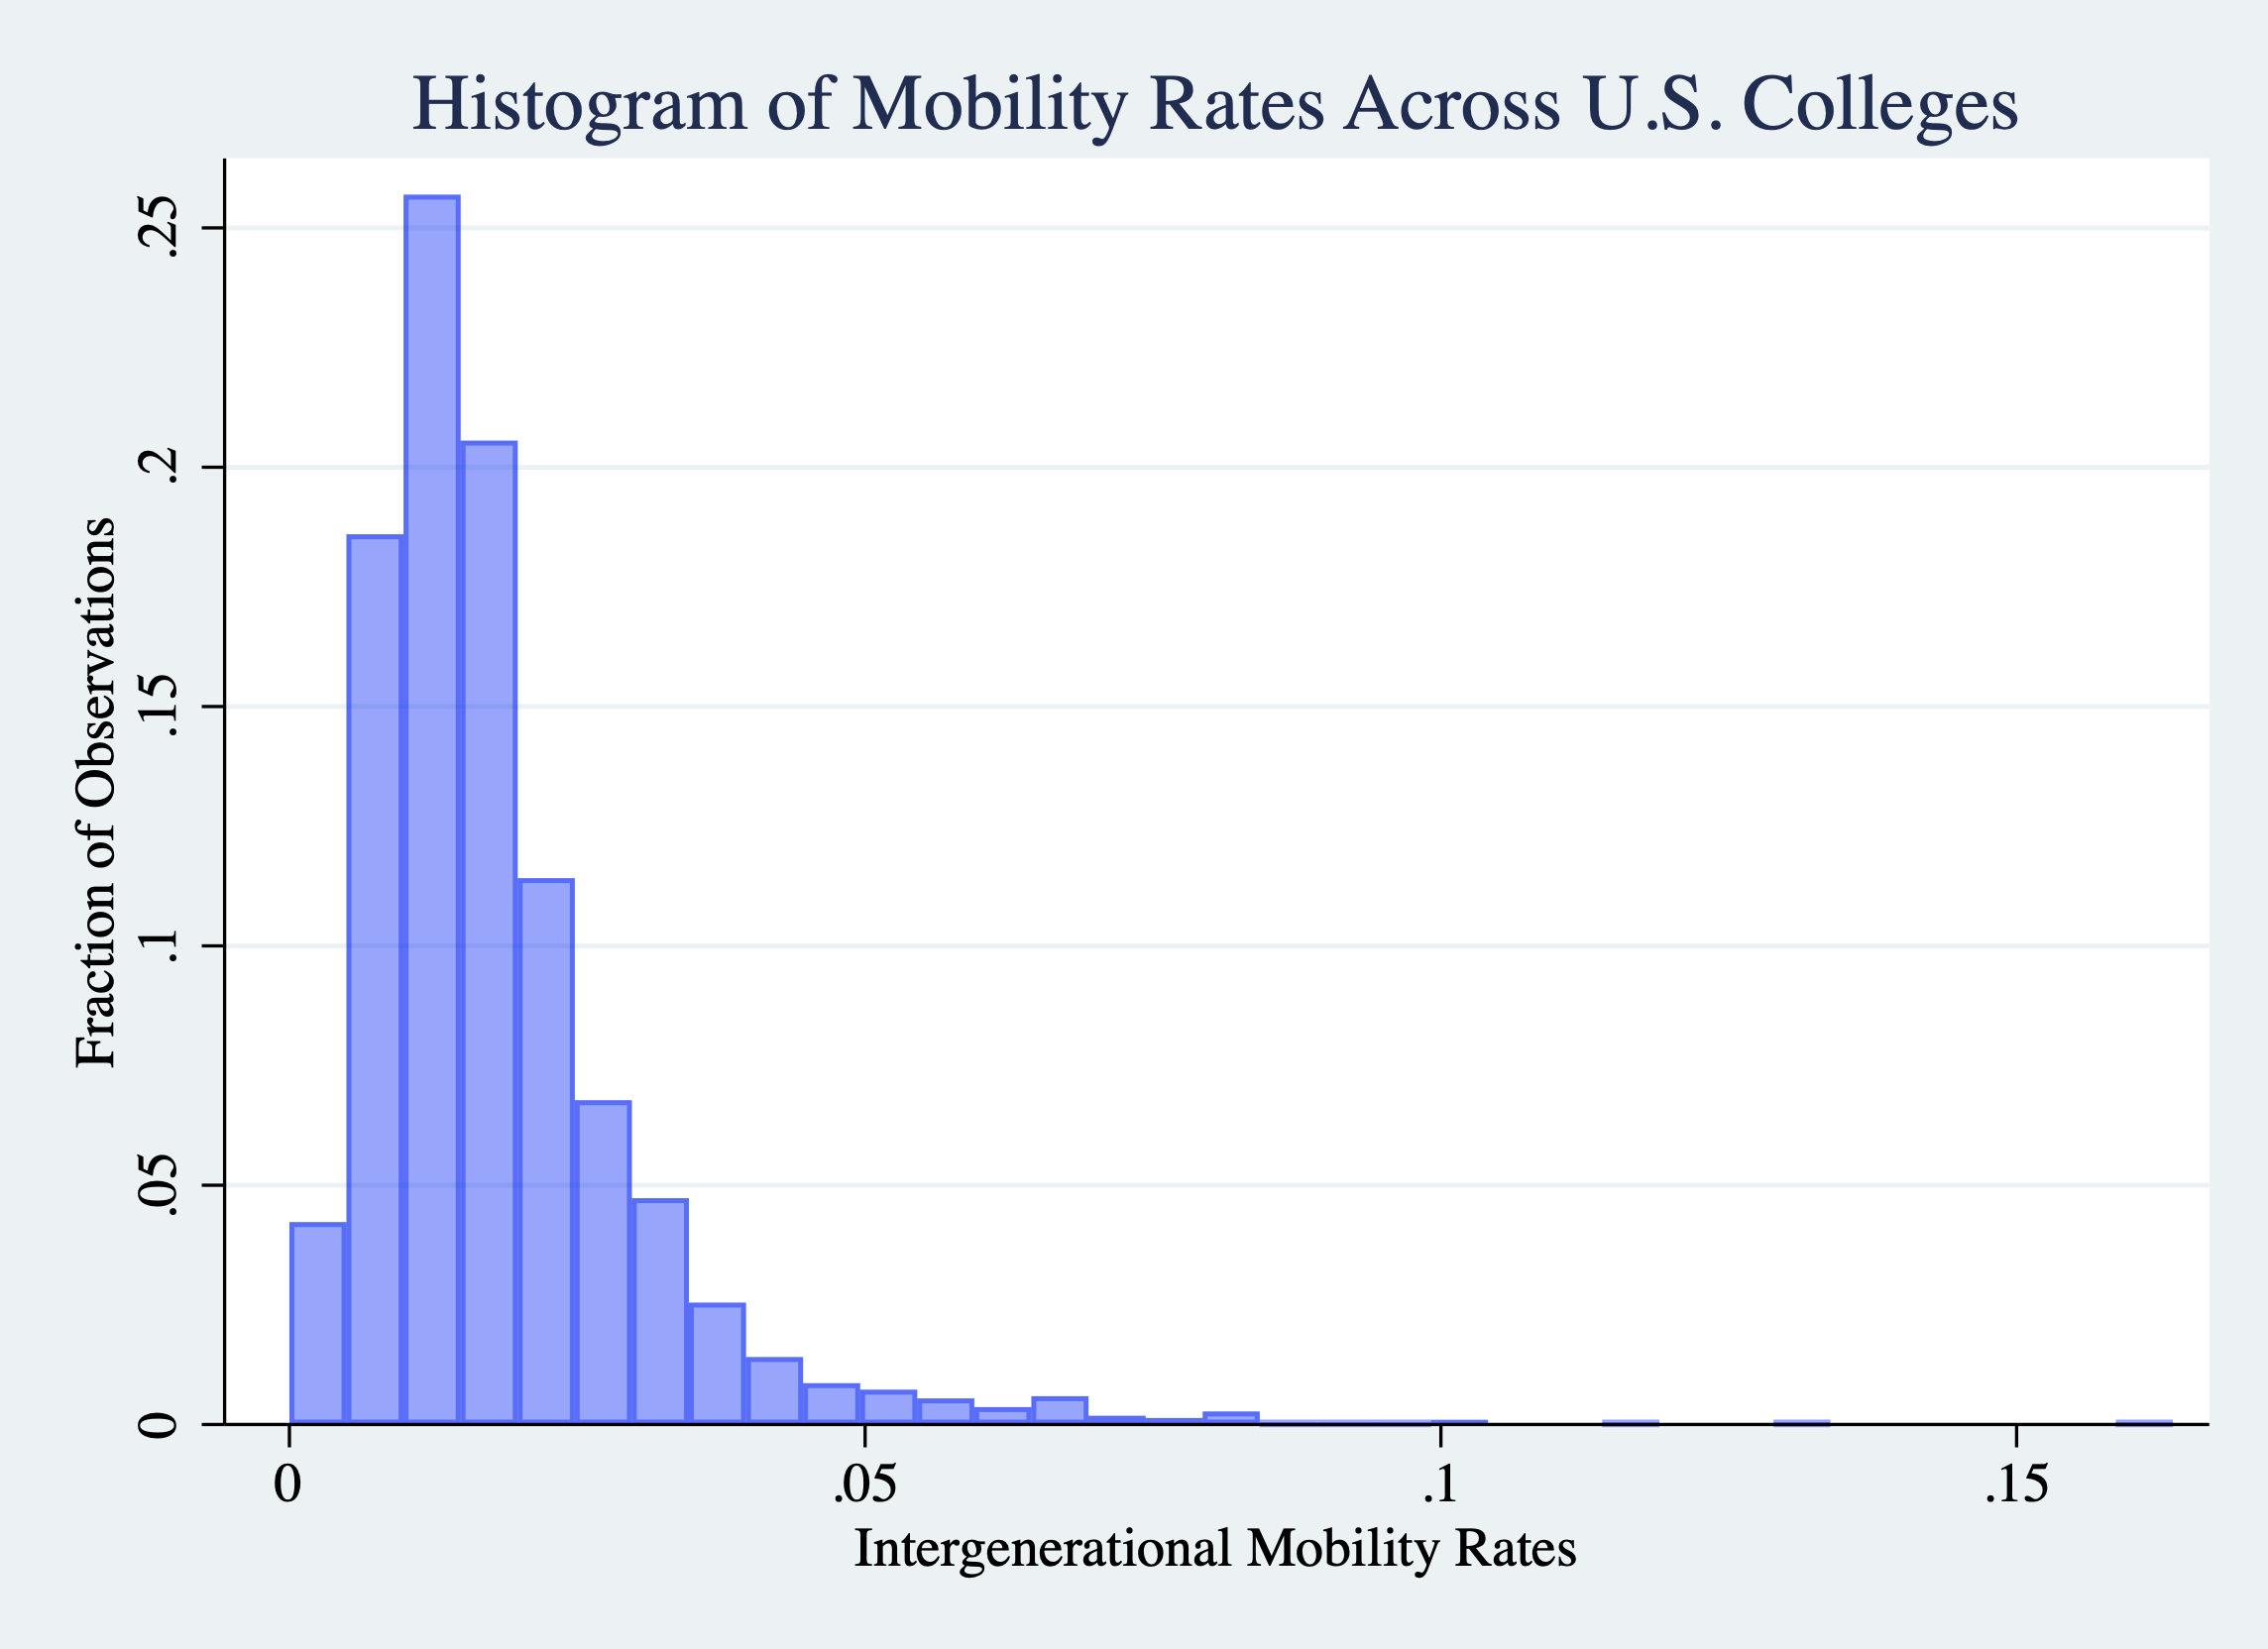
\includegraphics[width=0.85\linewidth]{images/02_histae4} 

}

\caption{Histogram of College Mobility Rates (Changing Axis Labels)}\label{fig:histae4}
\end{figure}

This next step is not strictly necessary, but I find the graphs more aesthetically pleasing if we also change the background color. We can do this by specifying \texttt{graphregion(fcolor(white))}

\begin{Shaded}
\begin{Highlighting}[]
\KeywordTok{histogram}\NormalTok{ mobility\_rate, frac }\KeywordTok{color}\NormalTok{(}\BaseNTok{blue}\NormalTok{\%40) }\CommentTok{///}
  \BaseNTok{title}\NormalTok{(}\StringTok{"Histogram of Mobility Rates Across U.S. Colleges"}\NormalTok{) }\CommentTok{///}
  \BaseNTok{xtitle}\NormalTok{(}\StringTok{"Intergenerational Mobility Rates"}\NormalTok{) }\CommentTok{///}
  \BaseNTok{ytitle}\NormalTok{(}\StringTok{"Fraction of Observations"}\NormalTok{) }\CommentTok{///}
\NormalTok{  graphregion(fcolor(}\BaseNTok{white}\NormalTok{)) }
\end{Highlighting}
\end{Shaded}

\begin{figure}

{\centering 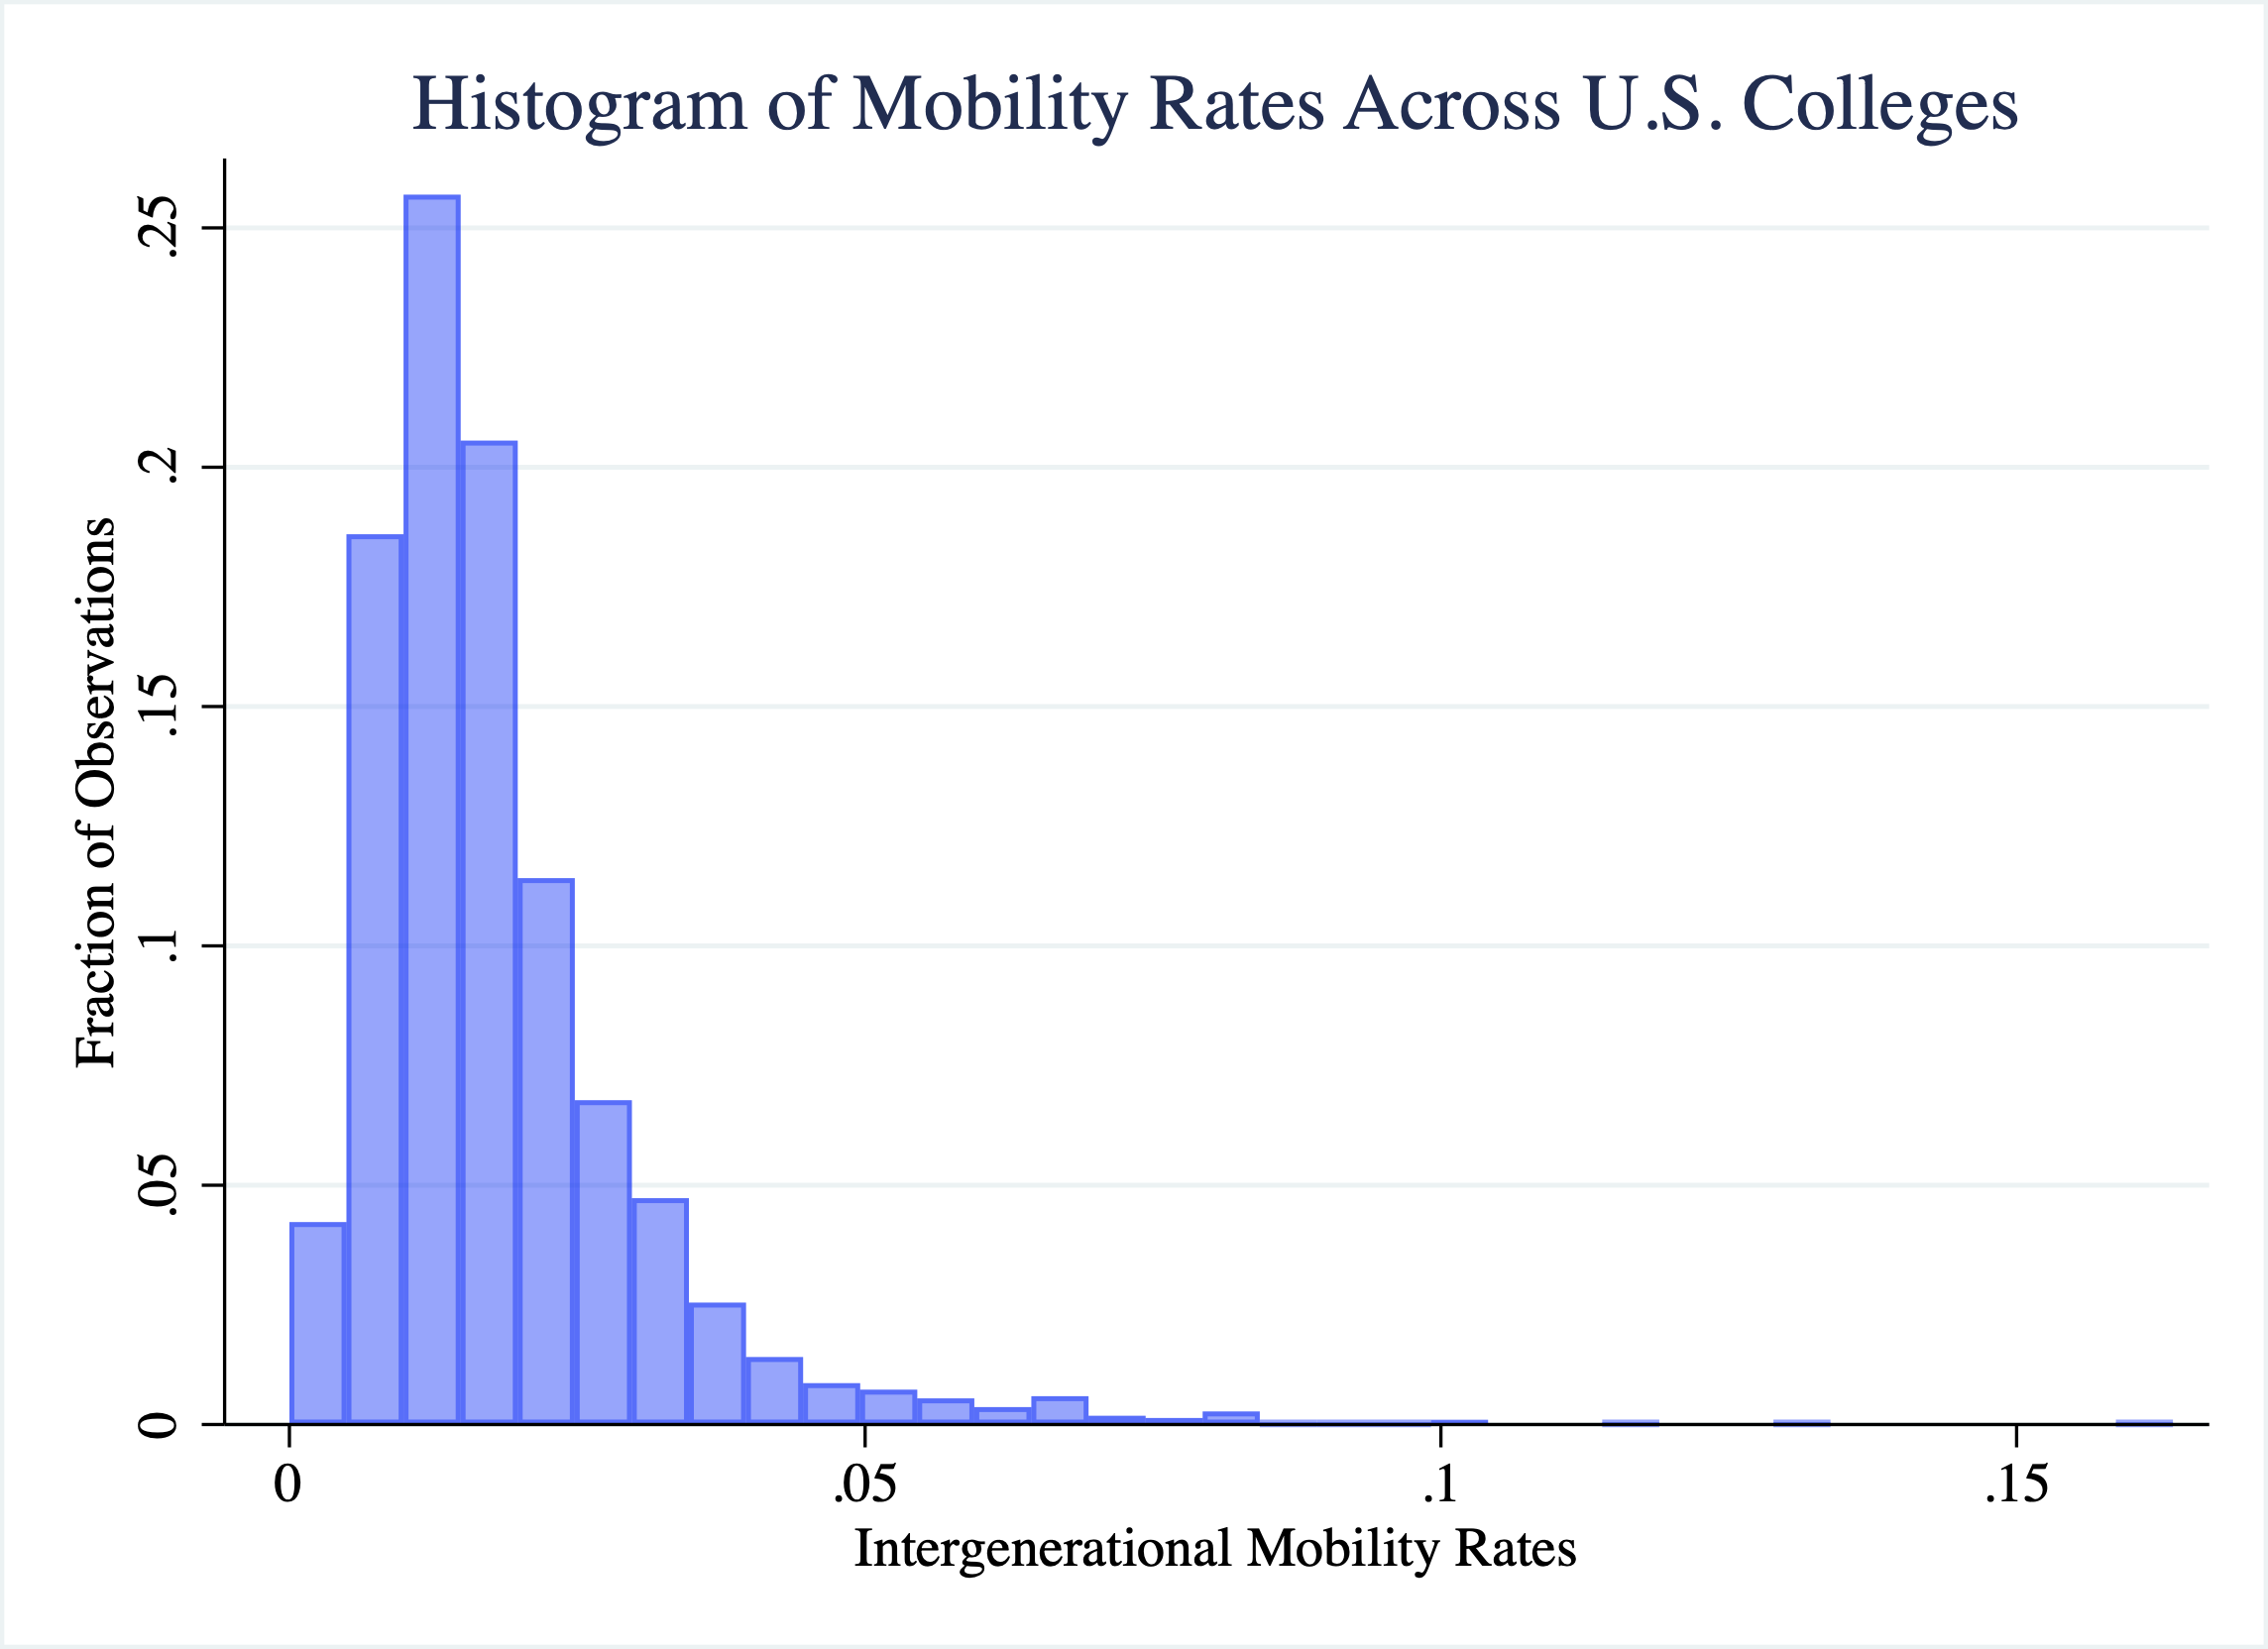
\includegraphics[width=0.85\linewidth]{images/02_histae5} 

}

\caption{Histogram of College Mobility Rates (Changing Background)}\label{fig:histae5}
\end{figure}

Sometimes it is helpful to highlight important elements in a graph. Let's add a vertical line at the mobility rate of UCSD, which is about 0.048. To do this we will add the \texttt{xline()} option to our figure. In particular, we will place a black line at 0.048 on the x-axis that is dashed by specifying \texttt{xline(0.048,\ lc(black)\ lp(dash))}. The option \texttt{lc(black)} specifies the line color (\texttt{lc}) will be black and \texttt{lp(dash)} indicates the line pattern (\texttt{lp}) will be dashed.

Further, we can also add text to the graph to label the dashed line. To add text, we use the \texttt{text()} option. In order to use the text option you need to specify the y-coordinate, the x-coordinate, and the text that should appear on the graph. For example, if we want to add the label UCSD, to the line we can add \texttt{text(0.2\ 0.055\ "UCSD")}. This will place the text \texttt{UCSD} at a value of \texttt{(y=0.2,x=0.055)} on the graph.

Figure \ref{fig:histae7} displays the plot that adds the vertical line and labels UCSD's mobility rate.

\begin{Shaded}
\begin{Highlighting}[]
\KeywordTok{histogram}\NormalTok{ mobility\_rate, frac }\KeywordTok{color}\NormalTok{(}\BaseNTok{blue}\NormalTok{\%40) }\CommentTok{///}
  \BaseNTok{title}\NormalTok{(}\StringTok{"Histogram of Mobility Rates Across U.S. Colleges"}\NormalTok{) }\CommentTok{///}
  \BaseNTok{xtitle}\NormalTok{(}\StringTok{"Intergenerational Mobility Rates"}\NormalTok{) }\CommentTok{///}
  \BaseNTok{ytitle}\NormalTok{(}\StringTok{"Fraction of Observations"}\NormalTok{) }\CommentTok{///}
  \BaseNTok{xline}\NormalTok{(0.048, lcolor(}\BaseNTok{black}\NormalTok{) lp(}\KeywordTok{dash}\NormalTok{)) }\CommentTok{///}
  \BaseNTok{text}\NormalTok{(0.2 0.055 }\StringTok{"UCSD"}\NormalTok{) }\CommentTok{///}
\NormalTok{  graphregion(fcolor(}\BaseNTok{white}\NormalTok{)) }
\end{Highlighting}
\end{Shaded}

\begin{figure}

{\centering 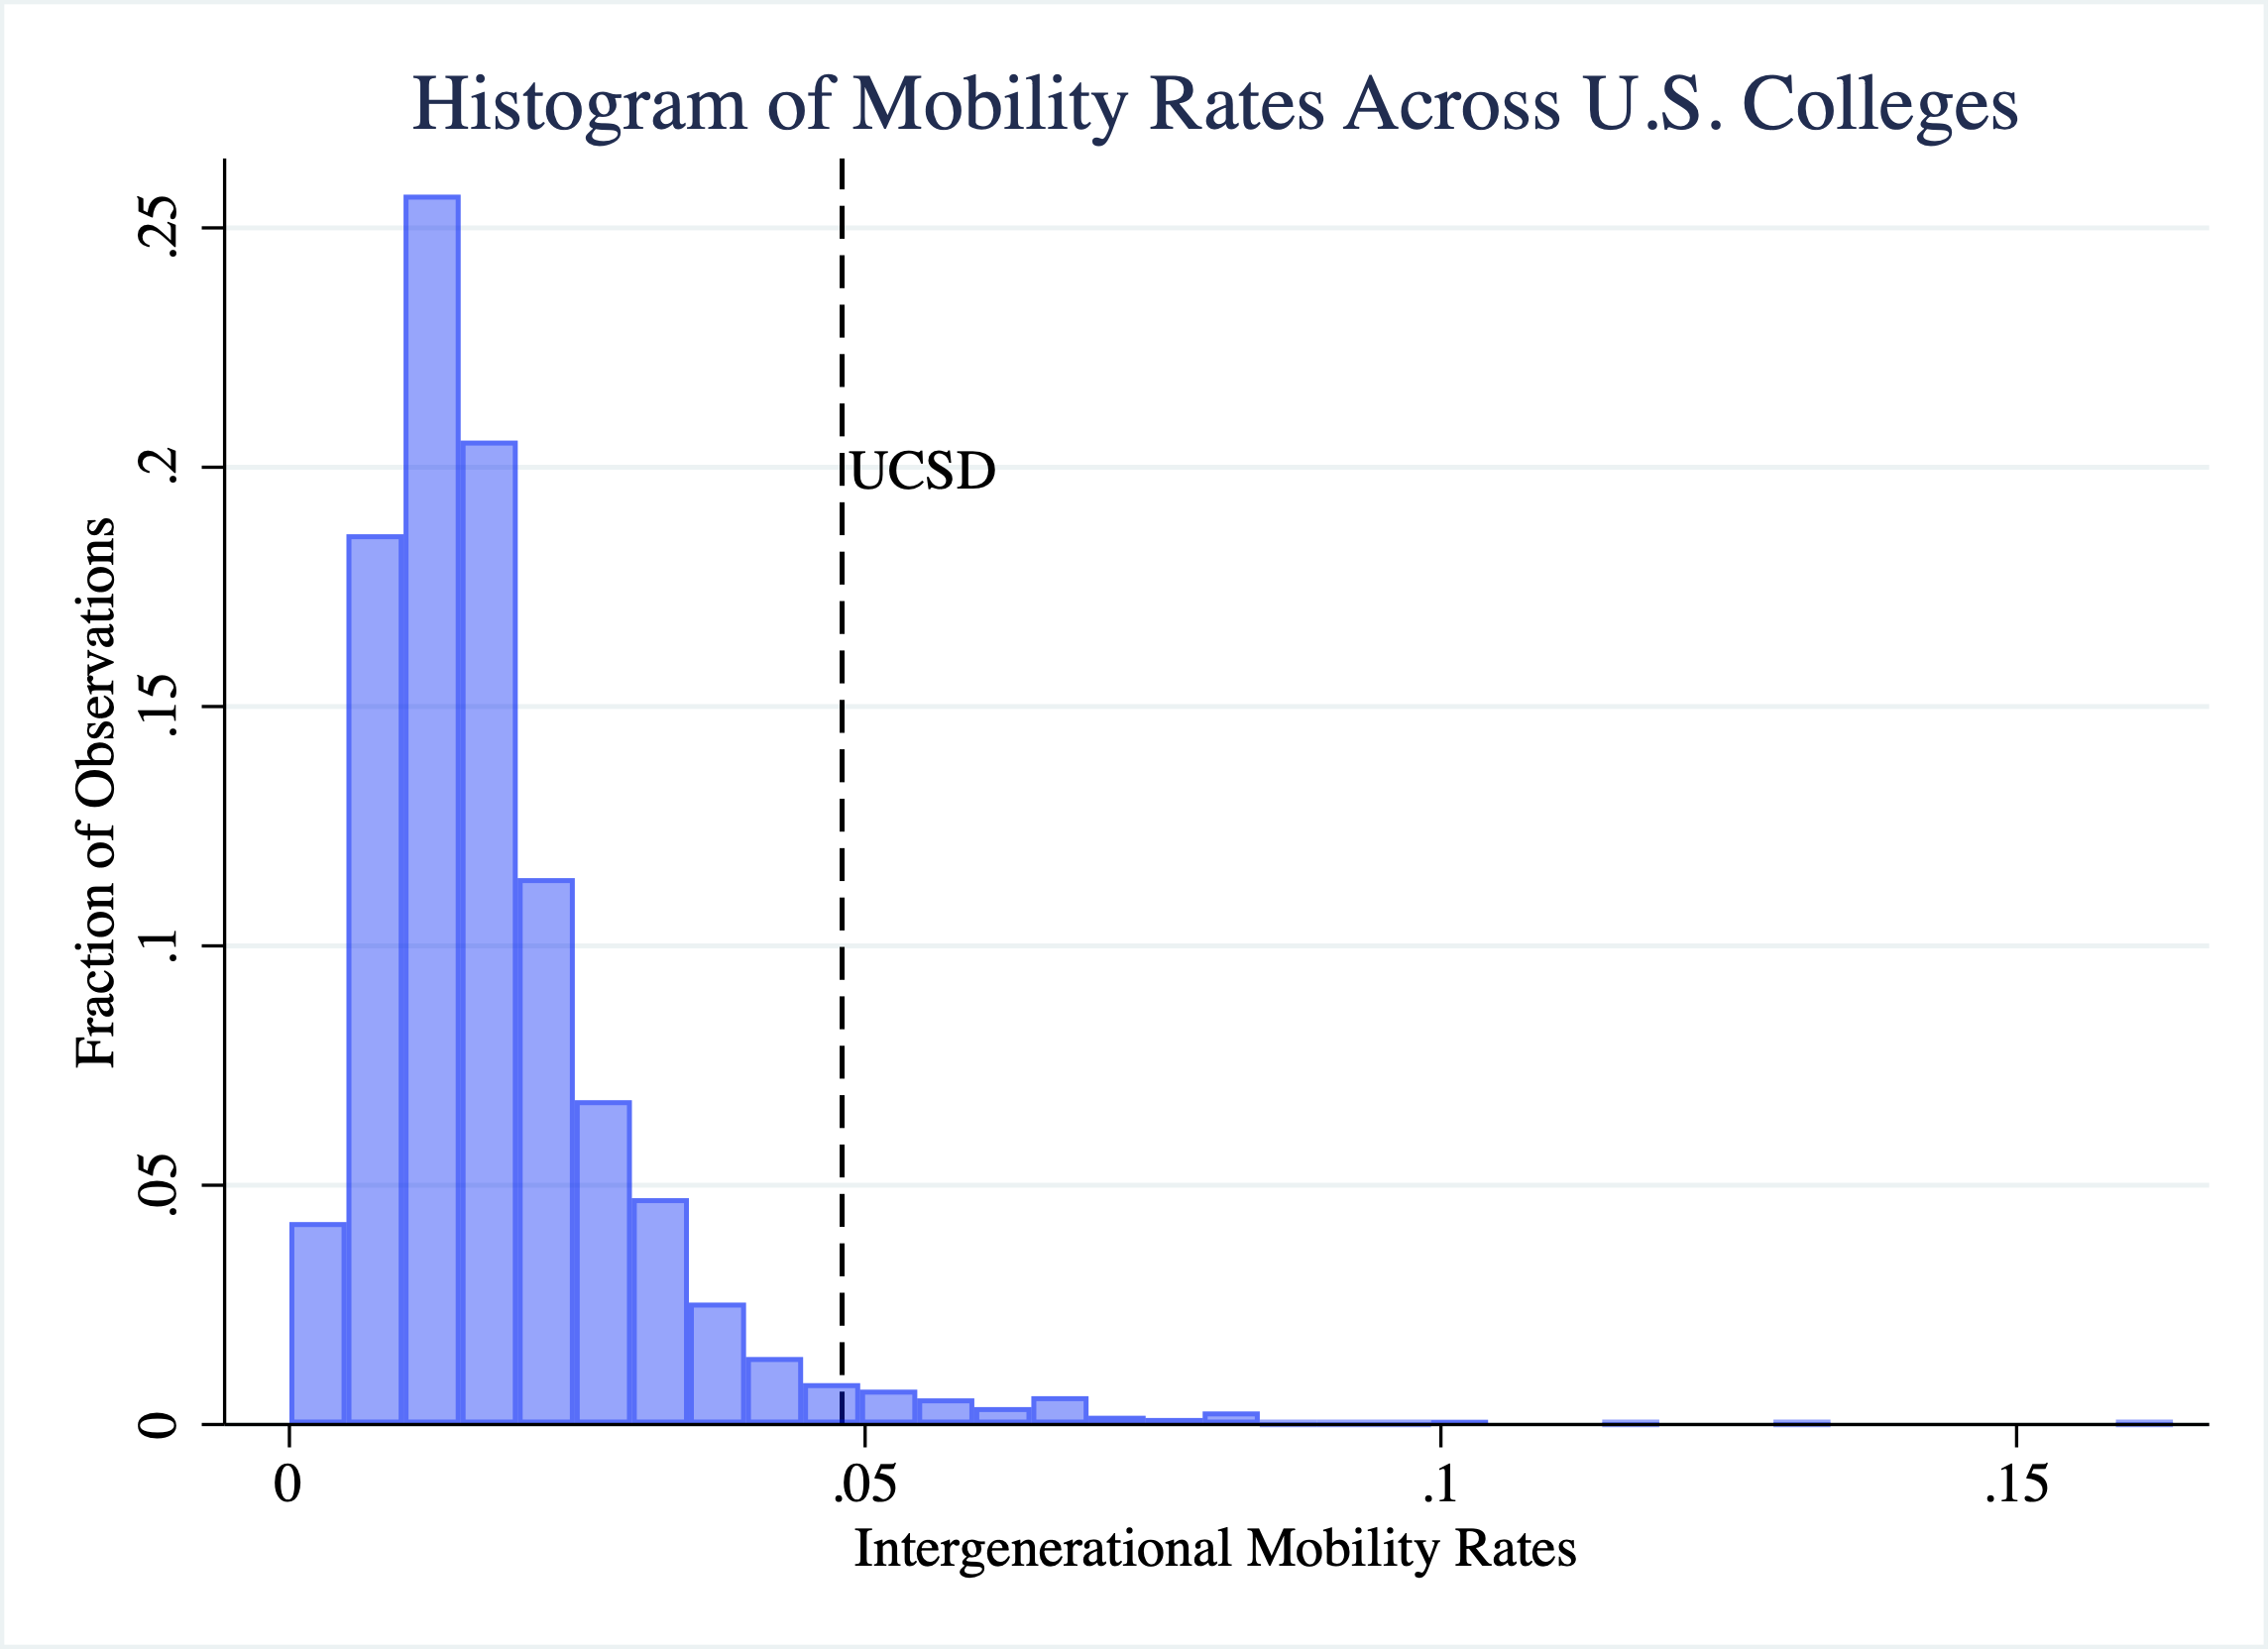
\includegraphics[width=0.85\linewidth]{images/02_histae7} 

}

\caption{Histogram of College Mobility Rates (Adding Vertical Line with Text)}\label{fig:histae7}
\end{figure}

\section{Conclusion}\label{conclusion}

In this module, we studied a college's intergenerational mobility rate. We found wide ranges of mobility rates across U.S. colleges. Some colleges have rates close to zero, which can be due to either (1) very low access to low-income students or (2) low success rates of students. Next, let's discuss what else we can learn from this data.

In Figure \ref{fig:avss} we plot both the access (fraction from low-income backgrounds) vs.~the success (percent of low-income students achieving high income).

\begin{figure}

{\centering 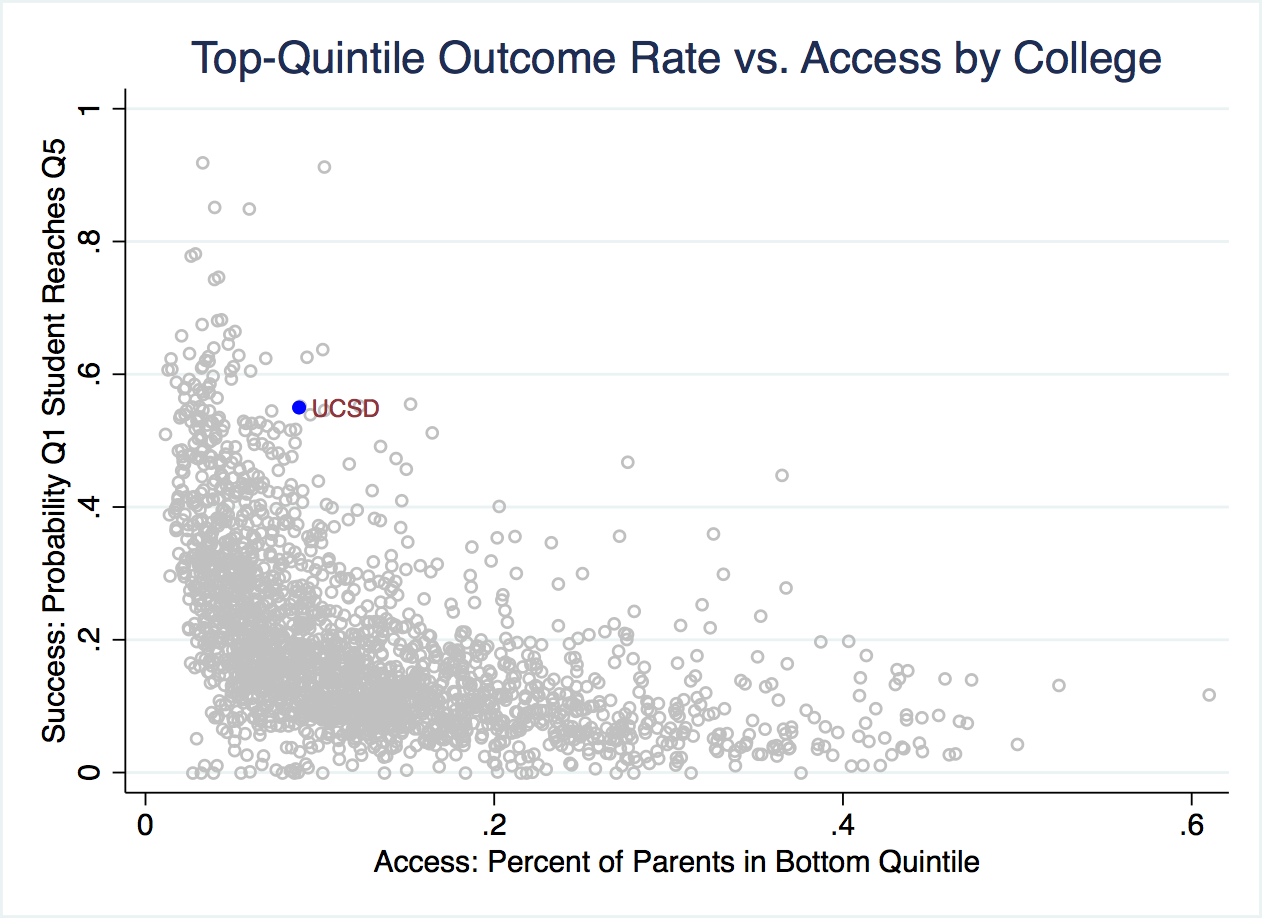
\includegraphics[width=0.85\linewidth]{images/02_scatter} 

}

\caption{Access vs. Success Across Colleges}\label{fig:avss}
\end{figure}

In Figure \ref{fig:avss}, rates of college mobility increase in both the vertical and horizontal axes. In other words, higher mobility rates are observed for colleges with both high access and success. As we can see in the figure, UCSD is highlighted. UCSD has a relatively high success rate. There aren't that many colleges with higher levels of success. However, its access rate is not particularly high. You can see that there are many many markers to the right of UCSD. This means there are many colleges with higher access than UCSD. The reason UCSD's mobility rate is relatively high is primarily due to its high success rate of graduates.

Although the data we used was a snapshot of a point in time, Opportunity Insights also has data about how colleges have been changing over time. Figure \ref{fig:ucsdaccess} plots the fraction of students coming from different quantiles of the income distribution over time.

\begin{figure}

{\centering 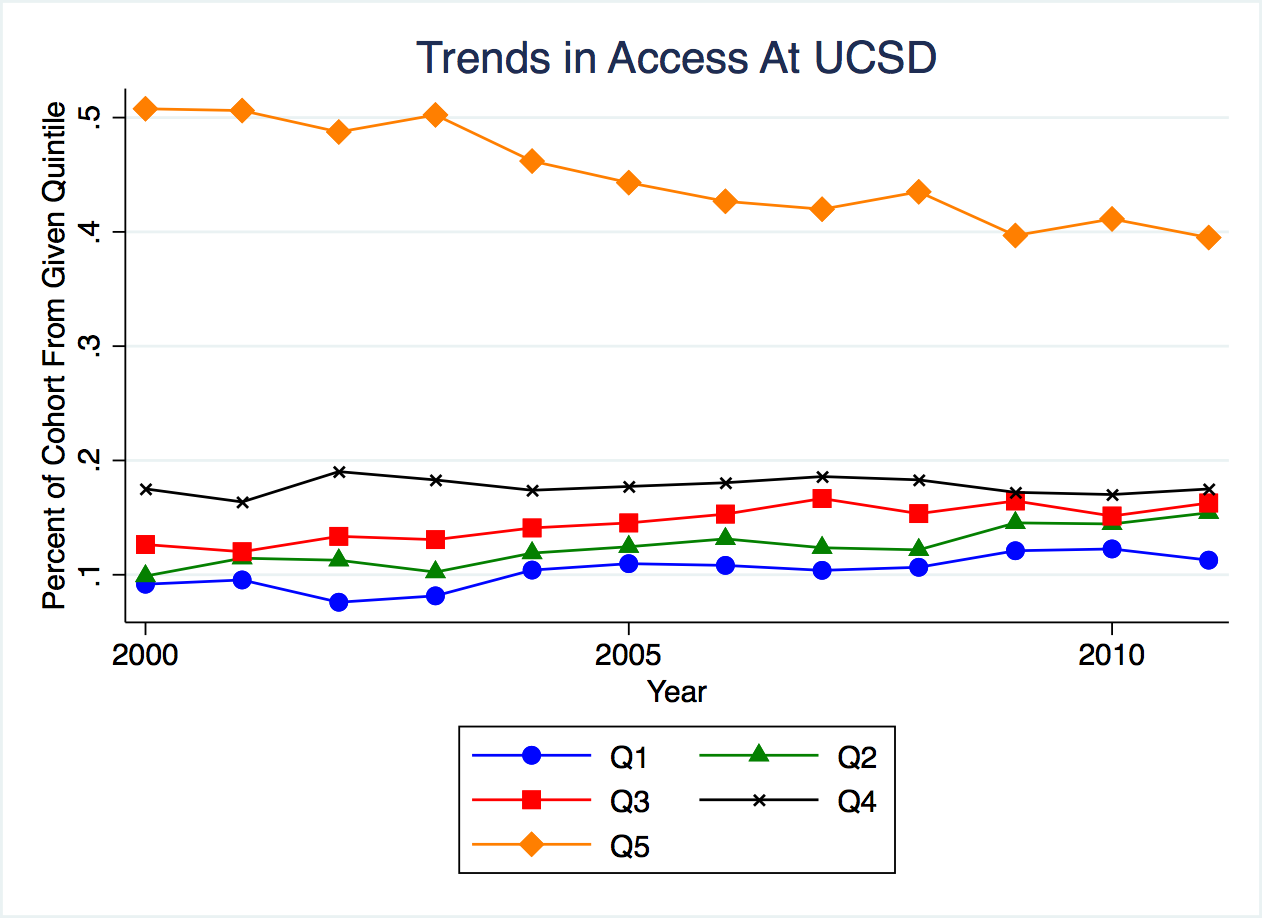
\includegraphics[width=0.85\linewidth]{images/02_trends} 

}

\caption{Trends in Access at UCSD}\label{fig:ucsdaccess}
\end{figure}

As can be seen in this figure, the fraction coming from Q5 (the top 20 percent of earners) is much greater than the other income quantiles. It starts at 0.5, indicating half of all students have parents in the top 20 percent of the income distribution. However, this number has been trending down over time. By 2013, the fraction coming from the top quintile has decreased to around 0.4 or 40 percent.

We can also plot a similar figure with success rates by quintile of parental income. Figure \ref{fig:ucsdsess} plots the success rate separately by the parental background of students.

\begin{figure}

{\centering 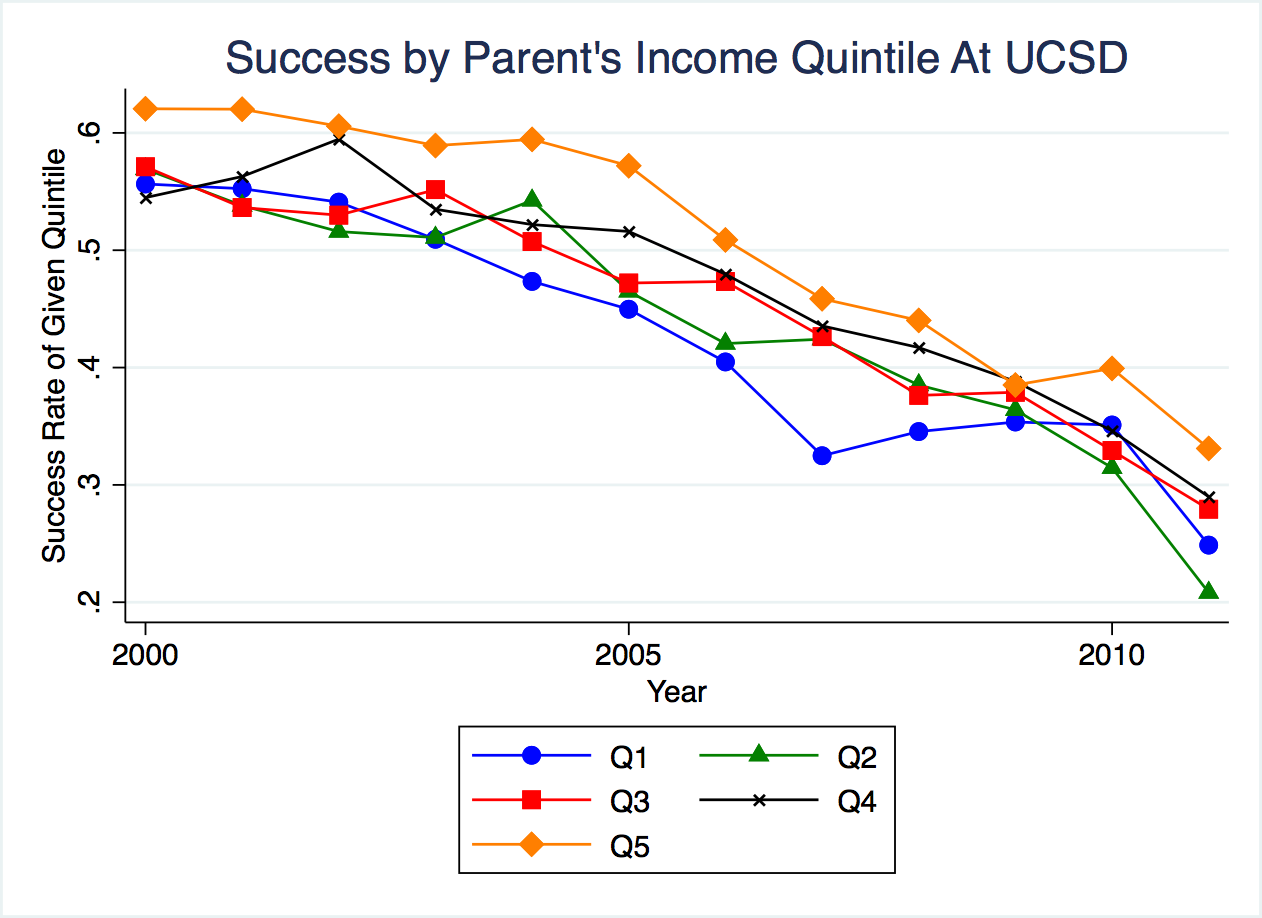
\includegraphics[width=0.85\linewidth]{images/02_trends2} 

}

\caption{Trends in Success at UCSD by Quintile}\label{fig:ucsdsess}
\end{figure}

As can be seen in this figure, different quantiles have relatively similar success rates. Researchers at Opportunity Insights study this across many different colleges, and find, on average, success rates are similar across the quintiles of parental background.

This works against a ``mismatch hypothesis'' that is sometimes discussed in policy circles. The hypothesis is that increasing access at elite universities to more lower-income students may not actually benefit these low-income students if they are unprepared for the curriculum. In other words, maybe it is better to go to a low-ranked school if there is a chance you will fail out of a higher-ranked school. But Opportunity Insights does not find evidence of this, on average. They find similar success rates for low-income and high-income students.

You will note in Figure \ref{fig:ucsdsess} success seems to be trending downward over time. This might be slightly misleading. Income in this data is measured in 2014. If UCSD students from recent cohorts are more likely to attend some form of graduate school, then earnings in 2014 might not reflect lifetime earnings. This could explain why there is a dip in these later cohorts.

UCSD had relatively high mobility rates but is far from the highest. Next, let's now look at the colleges with the highest mobility rates. Figure \ref{fig:topmobility} shows a list of schools with the highest mobility rates.

\begin{figure}

{\centering 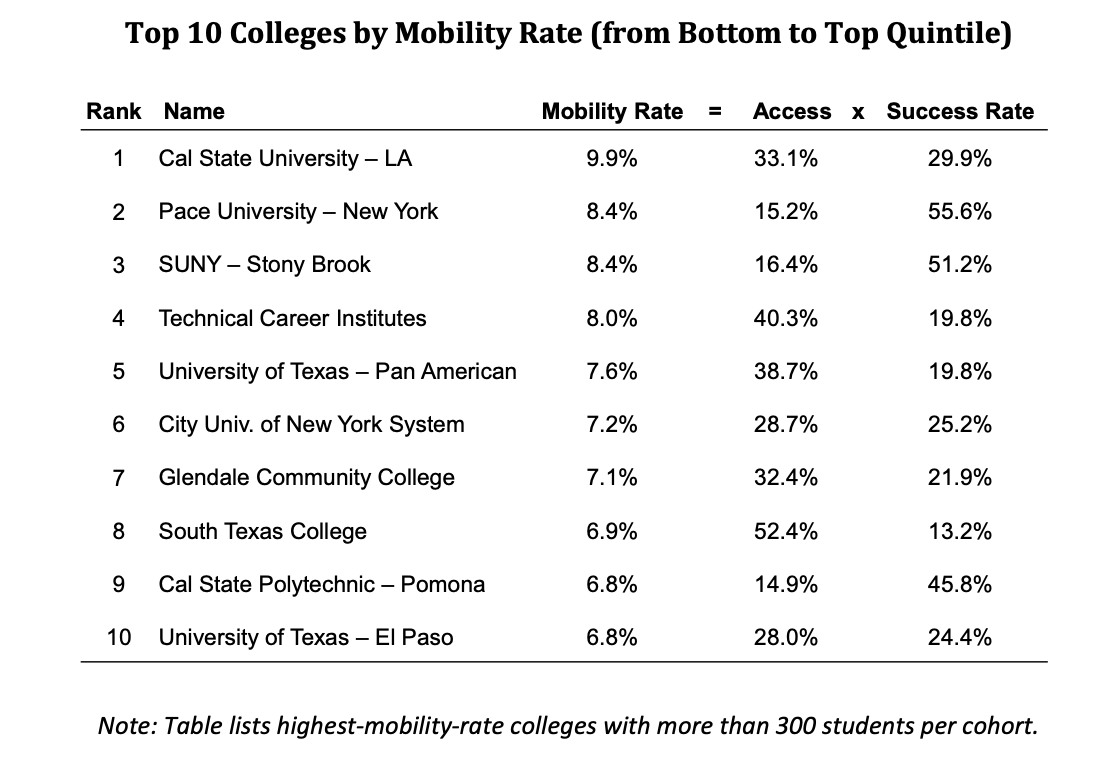
\includegraphics[width=0.85\linewidth]{images/02_top10} 

}

\caption{Schools with the Highest Mobility Rates}\label{fig:topmobility}
\end{figure}

What do many of these top schools have in common? They are mid-tier state schools. These schools appear very effective at promoting intergenerational mobility rates. The key is they tend to have high access rates, as well as reasonably high success rates. But how do trends in access look over time?

\begin{figure}

{\centering 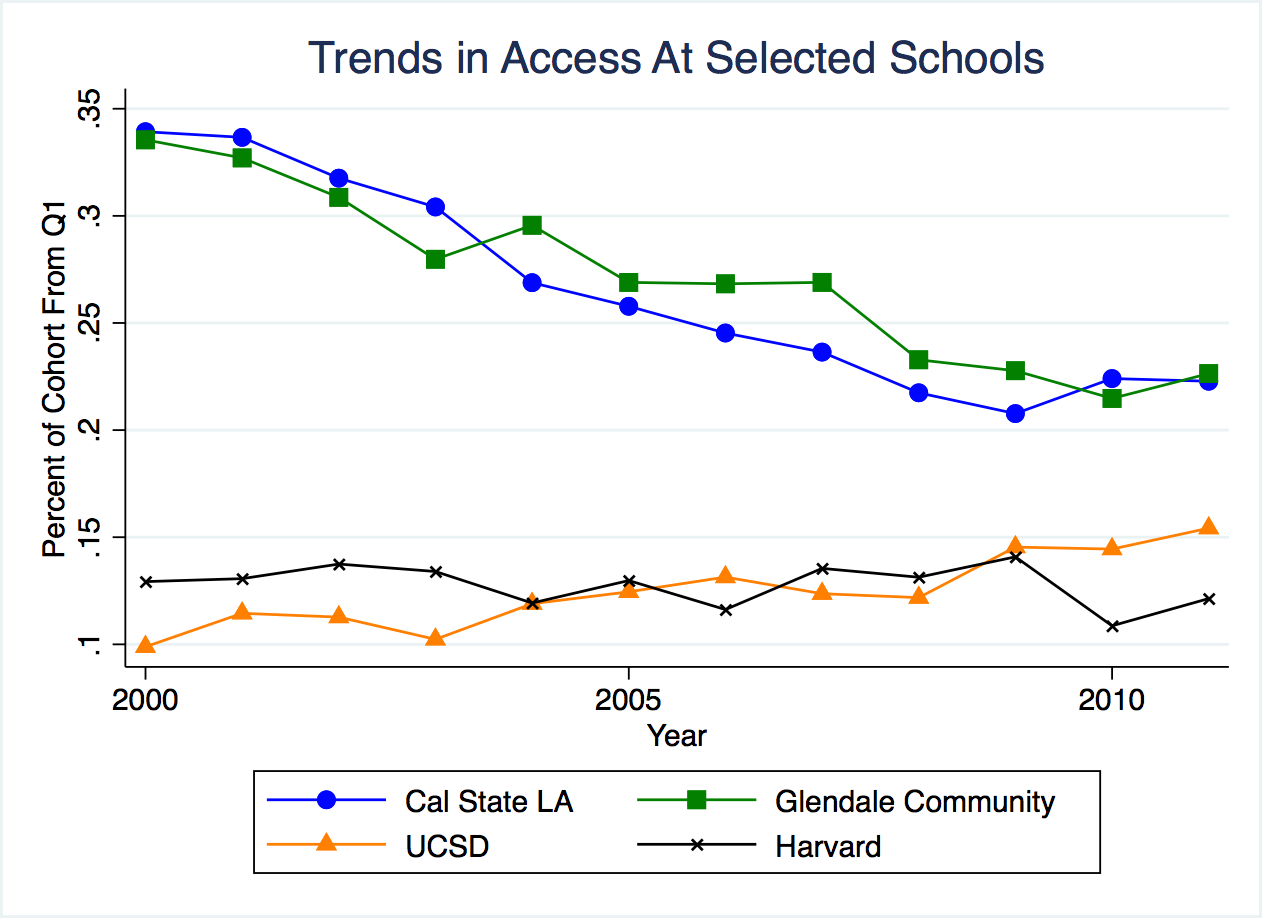
\includegraphics[width=0.85\linewidth]{images/02_trends_selected} 

}

\caption{Trends in Schools with the Highest Mobility Rates}\label{fig:trendstopmobility}
\end{figure}

Glendale and Cal State LA are two schools with very high mobility rates. But at these schools, the access rate is actually decreasing over time. In 2000 about 35 percent of students were coming from low-income backgrounds. In 2010, this has declined to a little more than 20 percent.

Before we end this module, let's discuss a few key takeaways from the researchers at Opportunity Insights. First, access varies widely by parental income, but success does not. Despite numerous policies aimed at increasing low-income enrollment at elite universities (e.g.~Harvard), we do not see increases in low-income enrollment over time at these universities

At the same time, many schools with very high access rates have been trending towards lower access in recent years. Opportunity Insights suggests changing admissions criteria or increasing transfers from community colleges could be effective policies in promoting intergenerational mobility (among other potential policy solutions).

\section*{Command Descriptions}\label{command-descriptions}
\addcontentsline{toc}{section}{Command Descriptions}

\textbf{Setup Commands}

\begin{itemize}
\item
  \texttt{cd\ filepath} -- this changes the working directory in Stata You should replace
  \texttt{filepath} with a file path of your choosing. If you have spaces in your file path, you need to put it into quotation marks.
\item
  \texttt{clear\ all} - clears data from Stata
\end{itemize}

\textbf{Data Exploration Commands}

\begin{itemize}
\item
  \texttt{describe} - describes the dataset and gives you information on the variables, types of variables, variable labels and number of observations.
\item
  \texttt{browse} - this opens up the data so that you can look at the values (like an excel spreadsheet).
\item
  \texttt{summarize\ varname} - retrieves summary statistics such as the mean, min and max for the variable named \texttt{varname}. To summarize all variables just type summarize. Add the option \texttt{,\ detail} to retrieve more statistics, such as percentiles.
\item
  \texttt{tab\ varname} - tab retrieves a table of frequencies. This can be used for string variables as well as categorical variables. For example, if you have a categorical named region, then the command \texttt{tab\ region} will display the number of observations in each region.
\end{itemize}

If you are trying to decide between \texttt{tab} and \texttt{summarize}, use \texttt{summarize} if the variable takes on many different values. Use \texttt{tab} if the variable takes on only a few values.

\textbf{Data Manipulation/Data Generation Commands}

\begin{itemize}
\item
  \texttt{gen\ newvar\ =\ exp} - \texttt{gen} is used to generate new variables. \texttt{newvar} is the name of the new variable, while \texttt{exp} denotes an expression. For example, if you want a new variable named \texttt{sum} which is the addition of \texttt{x1} and \texttt{x2} then you can type \texttt{gen\ sum\ =\ x1\ +\ x2}.
\item
  \texttt{replace\ var\ =\ exp} - replaces the values of variable \texttt{var} to the value in the \texttt{exp}. For example, if I have a numeric variable in which \texttt{-99} refers to missing values (as is sometimes the case in surveys). I can type \texttt{replace\ var\ =\ .\ if\ var==-99} to replace the variable to missing if the variable is currently equal to -99.
\end{itemize}

\textbf{Graphing Commands}

\begin{itemize}
\tightlist
\item
  histogram var, frac - computes a histogram (an approximation of the distribution of a continuous variable). There are many options to change the format of the graph. In this version of the code \texttt{,\ frac} is specified so that the vertical axis depicts the fraction of observations that fall within each bin.
\end{itemize}

\section*{References}\label{references}
\addcontentsline{toc}{section}{References}

\chapter{Discrimination in Police Stops}\label{discrimination-in-police-stops}

\section{SOPP Intro}\label{sopp-intro}

The most common way civilians interact with police is through traffic stops (there are about 50,000 a day). Given the frequency of encounters, detecting and eliminating racial discrimination in police behavior is an important policy goal. However, it can be difficult to detect without data. In this chapter, we will work with data from the Stanford Open Policing Project (SOPP). The SOPP is aggregating data on police stops across states and cities so that researchers, journalists and policymakers can improve interactions between police and the public. The data so far has information on about 200 million stops.

This is some big data. Figure \ref{fig:soppsnap} shows a subset of all the cities for which data has been collected.

\begin{figure}

{\centering 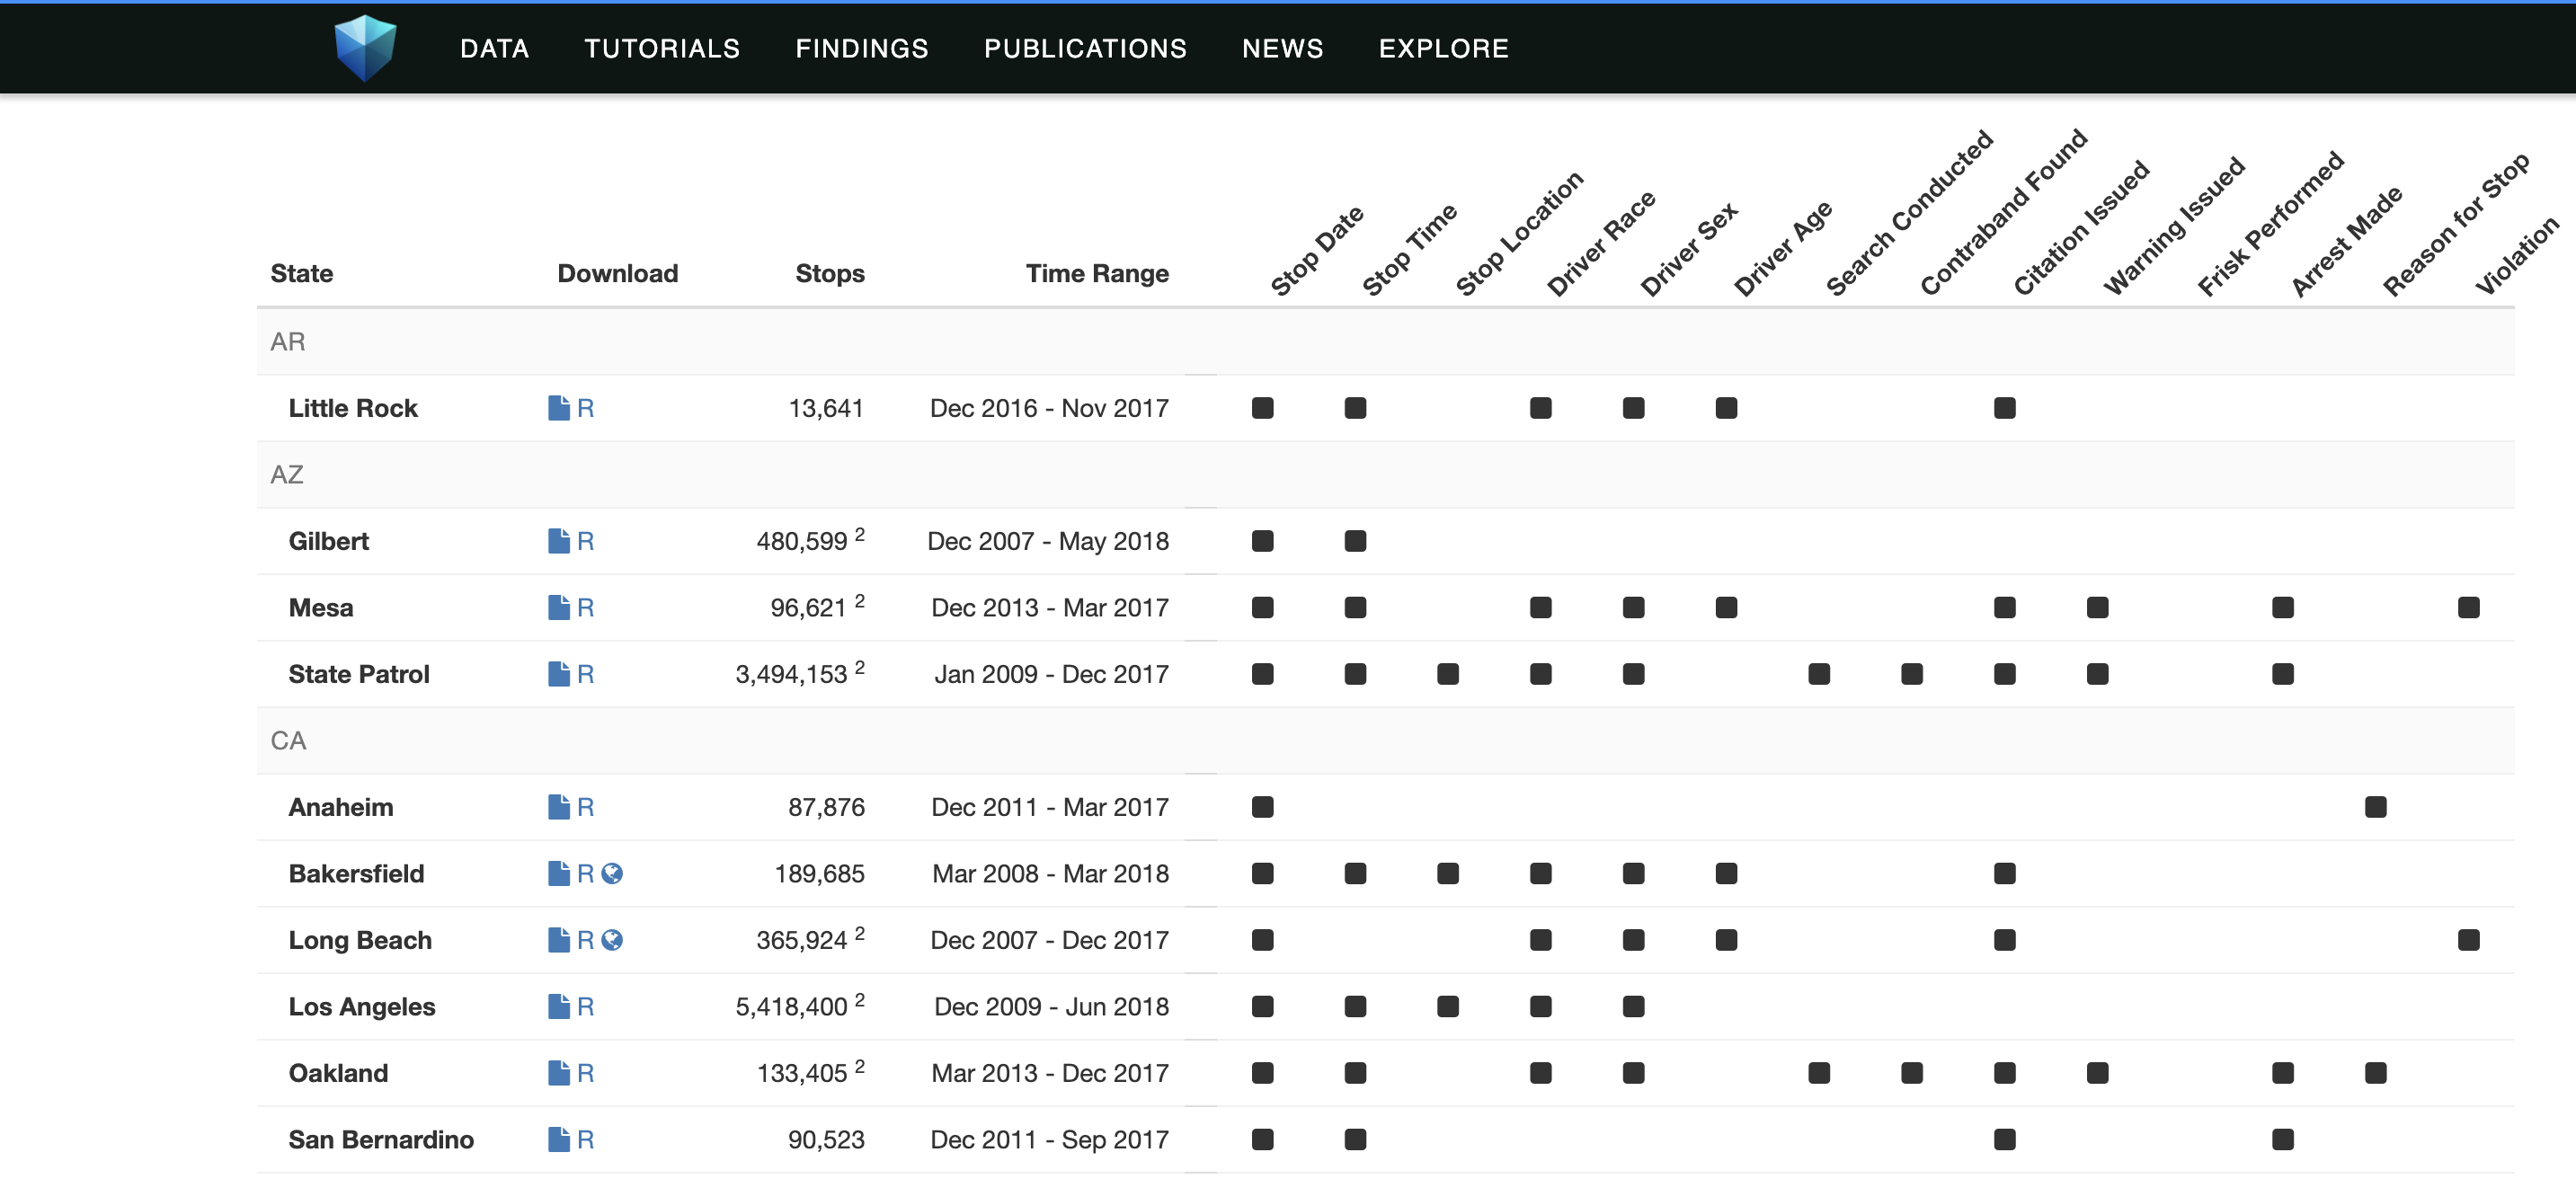
\includegraphics[width=0.9\linewidth]{images/03_data} 

}

\caption{The Stanford Open Policing Project Data}\label{fig:soppsnap}
\end{figure}

The data and research is starting to get noticed by many news outlets, including CNN, the Economist, the Huffington Post, NBC News and the Daily Show (see Figure \ref{fig:dailyshow})

\begin{figure}

{\centering 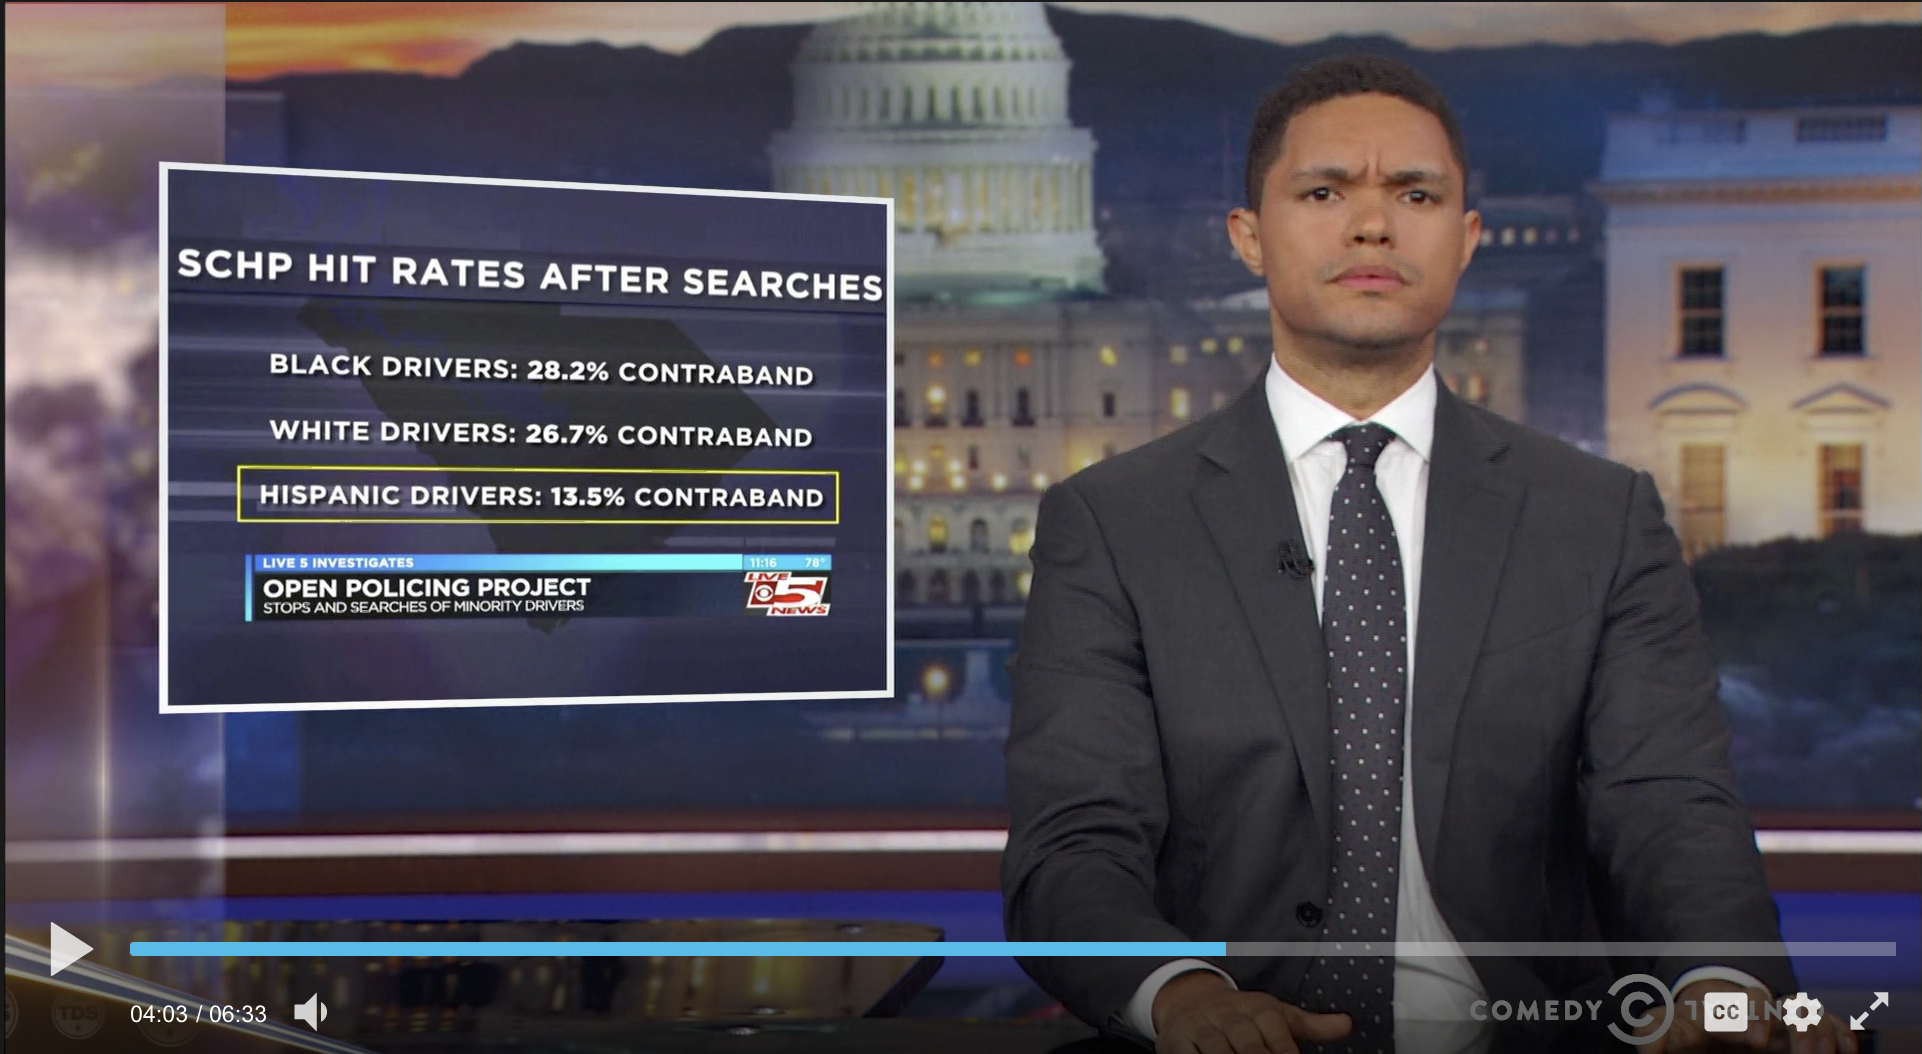
\includegraphics[width=0.7\linewidth]{images/03_daily_show} 

}

\caption{Trevor Noah Discussing Results from The Stanford Open Policing Project Data}\label{fig:dailyshow}
\end{figure}

There are many different ``decisions'' that officers make that could be driven by discrimination:

\begin{itemize}
\tightlist
\item
  \begin{enumerate}
  \def\labelenumi{\arabic{enumi}.}
  \tightlist
  \item
    The decision to stop a vehicle or not
  \end{enumerate}
\item
  \begin{enumerate}
  \def\labelenumi{\arabic{enumi}.}
  \setcounter{enumi}{1}
  \tightlist
  \item
    Conditional on stop, whether to issue a citation or not
  \end{enumerate}
\item
  \begin{enumerate}
  \def\labelenumi{\arabic{enumi}.}
  \setcounter{enumi}{2}
  \tightlist
  \item
    Conditional on stop, whether to search the car or not
  \end{enumerate}
\item
  \begin{enumerate}
  \def\labelenumi{\arabic{enumi}.}
  \setcounter{enumi}{3}
  \tightlist
  \item
    Conditional on stop, whether to arrest the individual or not
  \end{enumerate}
\end{itemize}

This data allows researchers to study all these potential margins for discrimination. Given the huge amount of data and the many margins that we could study, it will be helpful to narrow our focus. We will be studying \textbf{disparities in traffic stop rates} by the \textbf{race} of the motorists. Other possibilities would be to explore disparities in later stages of the traffic stops (citation/search/arrest) or other characteristics of the motorist (gender/age). Because the data is massive, we will focus on San Diego.

\section{SOPP Data}\label{sopp-data}

Now that we have narrowed our focus, let's start exploring the data for San Diego, as always we will need to set our working directory to where the data is located and then use the \texttt{use} command to load the data.

\begin{Shaded}
\begin{Highlighting}[]
\NormalTok{cd }\StringTok{"/Users/davidarnold/Dropbox/Teaching/EP5/online/03\_week/data"}
\KeywordTok{use}\NormalTok{ san\_diego\_stops.dta, }\KeywordTok{replace} 
\NormalTok{file gapminder.dta }\KeywordTok{not}\NormalTok{ Stata }\KeywordTok{format}
\FunctionTok{r}\NormalTok{(610);}


\NormalTok{/Users/davidarnold/Dropbox/Teaching/EP5/online/03\_week/}\KeywordTok{data}

\NormalTok{file san\_diego\_stops.dta }\KeywordTok{not}\NormalTok{ Stata }\KeywordTok{format}
\FunctionTok{r}\NormalTok{(610);}

\FunctionTok{r}\NormalTok{(610);}
\end{Highlighting}
\end{Shaded}

To begin, let's use \texttt{describe} to figure out what variables we have in this dataset

\begin{Shaded}
\begin{Highlighting}[]
\KeywordTok{describe}
\end{Highlighting}
\end{Shaded}

\begin{figure}

{\centering 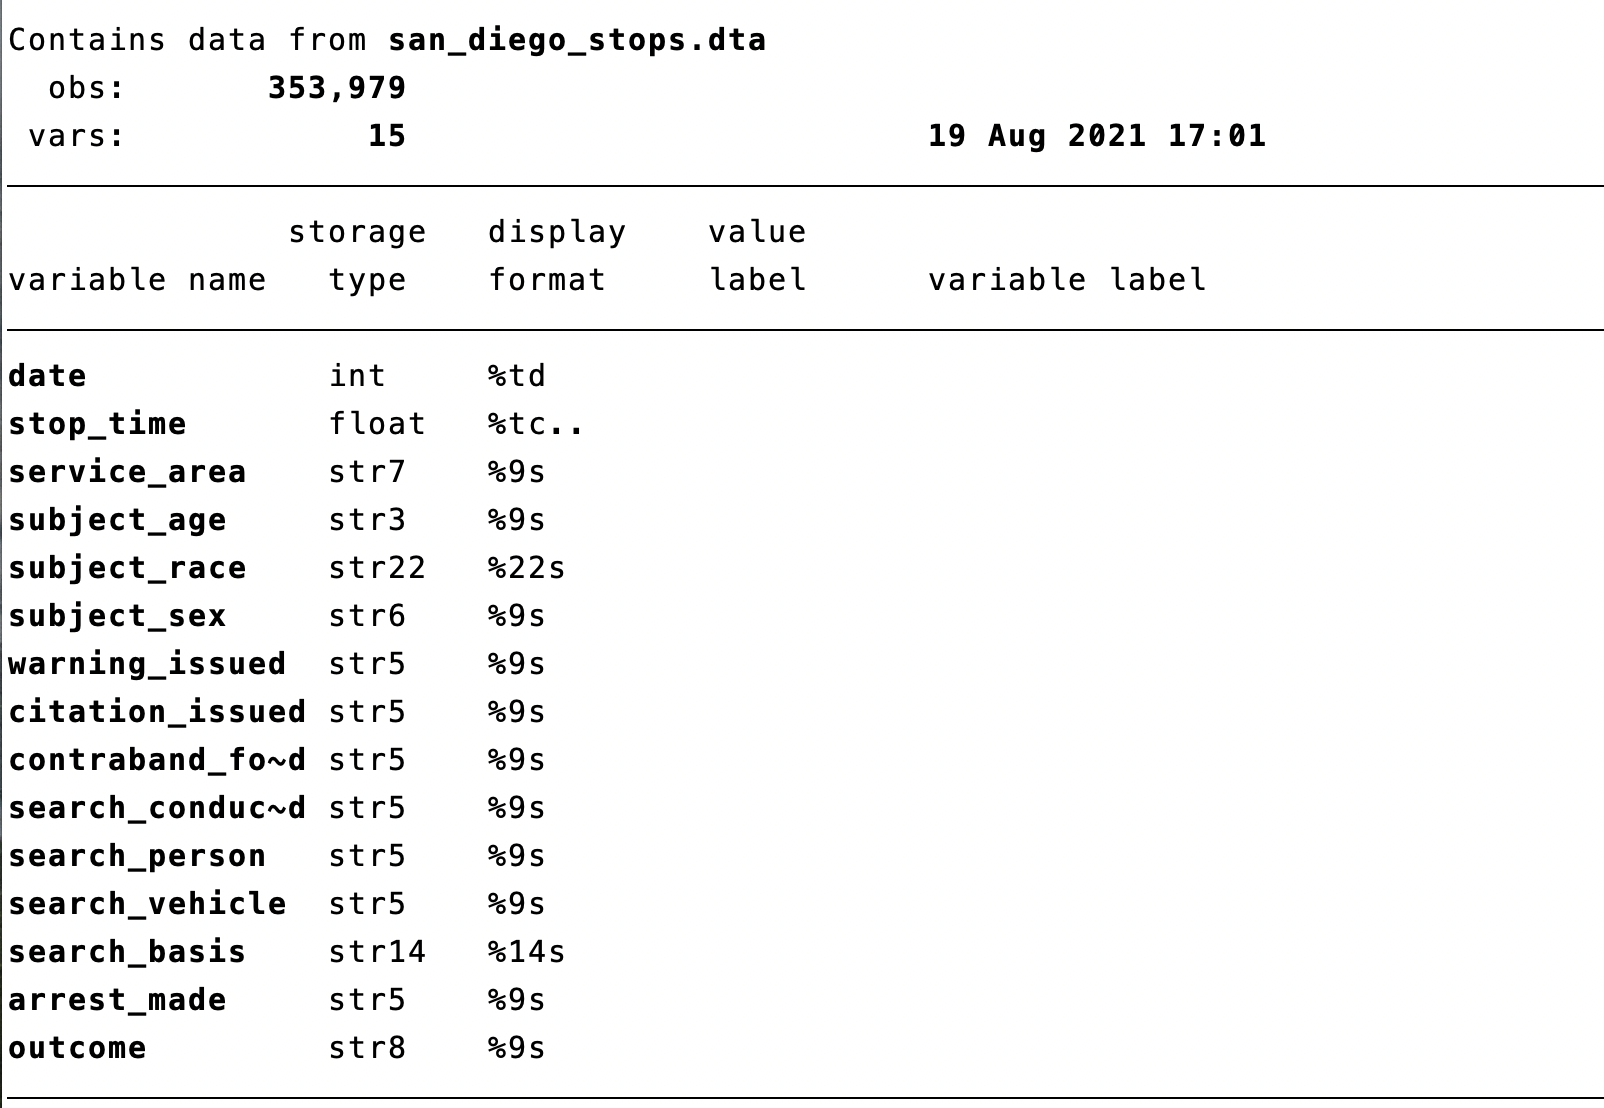
\includegraphics[width=0.9\linewidth]{images/03_describe} 

}

\caption{San Diego Stops Data from Stanford Open Policing Project Data}\label{fig:sandiegostops}
\end{figure}

Each observation in the dataset is a stop made by an officer somewhere in San Diego. \texttt{stop\_time} contains the time of the stop. Remember this variable, we will return to it later. Our goal is to understand if there is discrimination in who is stopped. Therefore, we will be frequently using the \texttt{subject\_race} variable in our dataset.

Subject race is a \textbf{categorical variable}. Whenever you have a categorical variable as your variable of interest, it is helpful to understand the frequency of each category. For example, what fraction of stops are for Black drivers, White Drivers, Hispanic Drivers, etc. To do this in Stata, we will use the \texttt{tab} command.

\begin{Shaded}
\begin{Highlighting}[]
\KeywordTok{tab}\NormalTok{ subject\_race}
\end{Highlighting}
\end{Shaded}

\begin{verbatim}
file gapminder.dta not Stata format
r(610);


no variables defined
r(111);

r(111);
\end{verbatim}

This gives us the fraction of stops by race in San Diego. To begin to understand whether there is a disparity in traffic stops by race, we can compare the composition of traffic stops to the overall population to see if certain groups are over/underrepresented \medskip

\begin{figure}

{\centering 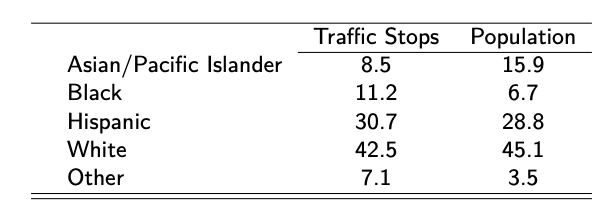
\includegraphics[width=0.8\linewidth]{images/03_population} 

}

\caption{Racial Composition of Traffic Stops and Population}\label{fig:population}
\end{figure}

As can be seen in Figure \ref{fig:population}, Black drivers are over-represented in police stops. 11.2 percent of all stops are Black drivers while 6.7 percent of the population is Black. Asian/Pacific Islanders are underrepresented in traffic stops (8.5 percent of stops vs.~15.9 percent of the population). Hispanic drivers are slightly overrepresented in traffic stops (30.7 percent of stops vs.~28.8 percent of the population) while White drivers are slightly underrepresented (42.5 percent of stops vs.~45.1 percent of the population). One important caveat is that demographic information is from the 2010 Census, while traffic stop data is from 2014-2017. Therefore, these numbers may not be directly comparable if demographics are changing over time in San Diego.

However, this analysis does present some striking disparities in traffic stops. These disparities will be the focus of our analysis in this section. In particular, we will learn one test that can be used to understand whether these disparities are driven by racial discrimination on the part of police officers.

\section{Veil of Darkness (VOD)}\label{veil-of-darkness-vod}

Racial disparities refer to any differences between groups of different races. Many factors can cause racial disparities, but a common focus is to try to understand if the disparity is driven by racial discrimination. In our example, we are interested in exploring racial discrimination on the part of police officers making traffic stops. Many methods have been proposed to prove racial discrimination. Today we focus on one: \textbf{the veil of darkness test}, a test developed by Grogger and Ridgeway (2006)\citep{grogger2006testing}.

The basic idea behind the veil of darkness test is that it easier to observe the race of an individual driver during the day when there is sunlight relative to the night when it is dark. Therefore, if police officers are targeting minority drivers, then it will be more difficult to perform this targeting at night. We can therefore compare the racial composition of traffic stops during daylight vs.~nighttime to try to infer racial discrimination on the part of police officers.

In Figure \ref{fig:veil1} the basic assumptions behind the veil of darkness test are presented. Before sunset, it is light out, and officers can observe the race of drivers. After sunset (but before dusk), it is unclear whether race is observed or not. After dusk, however, we assume officers can no longer observe race before deciding to stop a given driver.

\begin{figure}

{\centering 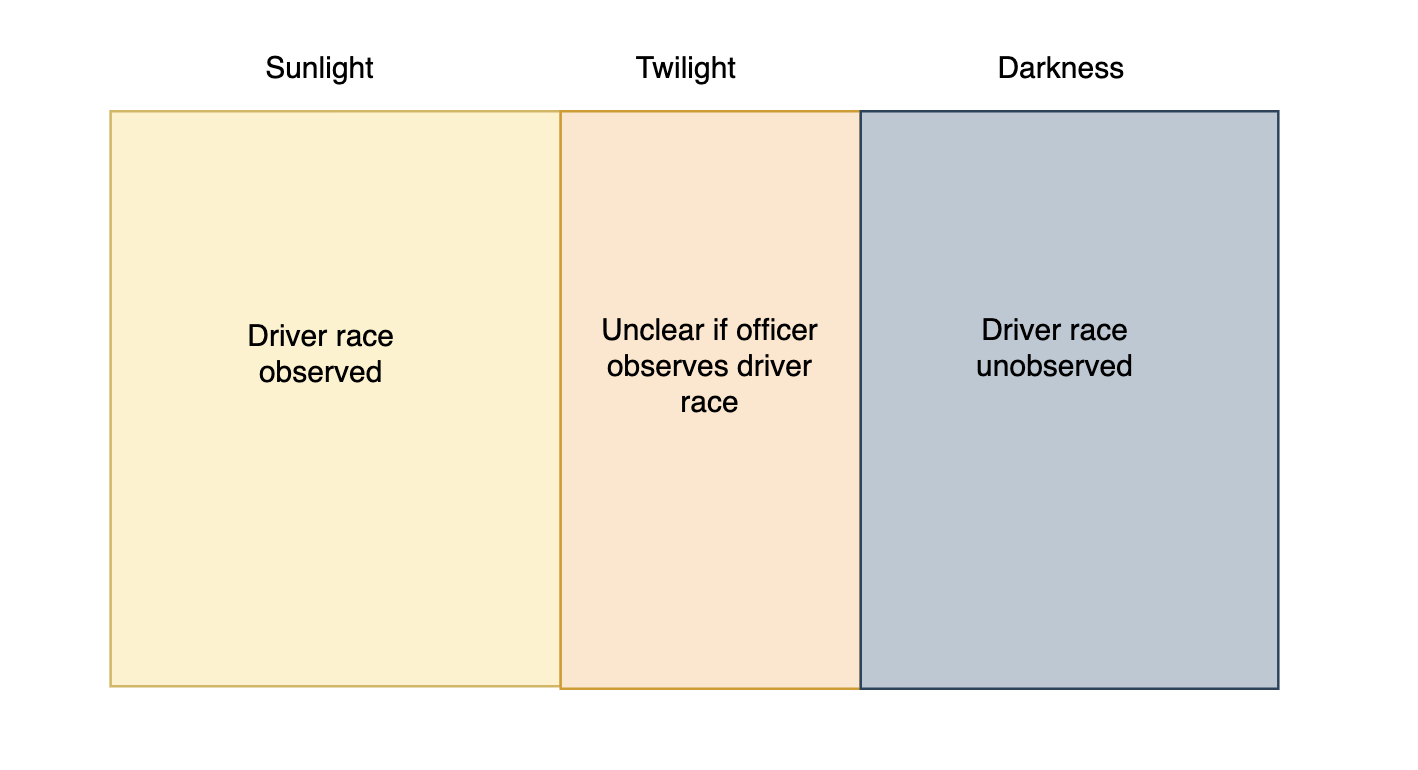
\includegraphics[width=0.75\linewidth]{images/03_veil1} 

}

\caption{Assumptions Behind Veil of Darkness Test}\label{fig:veil1}
\end{figure}

In the data, imagine we see stops for a given type of drive fall dramatically after dusk. This might suggest that officers were targeting these individuals before dusk. But before we make any firm conclusions, we need to think carefully about comparing across different times in the day.

For example, at 12 noon it is light out. At 12 midnight it is dark out. However, there are many differences between 12 noon and 12 midnight. The drivers on the road are probably completely different. Therefore, if the racial composition of stops is different at these times, maybe it is not due to the officers, but due to the drivers on the road.

To get around this issue, Grogger and Ridgeway (2006) focus on the intertwilight period, which are times in which it is sometimes light out and sometimes dark.

For example, at 6:30 PM it is sometimes light out in San Diego (in the summer). However, at different times of year (in the winter) it is dark out at 6:30 PM. Therefore, maybe we can compare the composition of traffic stops around 6:30 PM in the summer and the winter to understand whether police officers are more likely to stop minority drivers when it is light out.

For example, imagine 40 percent of drivers stopped are Black when it is light out (at 6:30 PM), but 35 percent of drivers stopped are Black when it is dark out (still 6:30 PM, but a different part of the year). In this hypothetical example, the decrease in stops for Black drivers must be due to officers' inability to racially profile when it is dark.

If you recall, in our data we have information on the time a given traffic stop occurred, as well as the race of the driver. However, we also need to have information on whether it was light or dark at the time of that given stop. To add this to our dataset we will need to \textbf{merge} in external data on sunset times. This will introduce us to \textbf{data wrangling} in Stata

\section{Data Wrangling}\label{data-wrangling}

When you start an empirical research project in the social sciences, you must ask the question: what data can I use to answer this question? Once you have identified the data, it rarely comes in a format that is ready for data analysis. Generally, there are a number of steps that must be taken to prepare the data. These steps are often referred to as \textbf{data wrangling}

For example, the Census has confidential income data that is available only to researchers who go through an application process. The data, however, is stored separately for every state. To create a master dataset, you would need to combine all these individual datasets. This is a form of data wrangling. In Stata, this is accomplished with the \textbf{append} command

Next, imagine you are interested in the relationship between economic conditions and the opioid crisis in the United States. The Bureau of Labor Statistics provides county-level information on unemployment. The Centers for Disease Control and Prevention (CDC) provides county-level opioid prescription data. To study this question, we would need to combine these two datasets together at the county level. This is another example of data wrangling, and in Stata, this is accomplished with the \textbf{merge} command.

Lastly, imagine you have individual-level data on voting rates, but you are interested in comparing voting rates across counties. In other words, it would be more convenient for your analysis to have a dataset at the county level, rather than at the individual level. This is another example of data wrangling, and in Stata, this can be accomplished with the \textbf{collapse} command.

In this section, we will learn about all three of these commands: append, merge, and collapse, with a particular focus on (1) when each is appropriate and (2) how we implement them in Stata.

\section{Append}\label{append}

The \texttt{append} command is used when you want to \textbf{add rows} to a dataset. This is common in many situations. For example, it is common that datasets are stored separately for each year, but you want to analyze data across years. It is also common for datasets that are stored separately for each region but you want to analyze data for the entire country.

To understand how to use the append command we will consider a simple hypothetical example depicted in Figure \ref{fig:appendhyp}.

\begin{figure}

{\centering 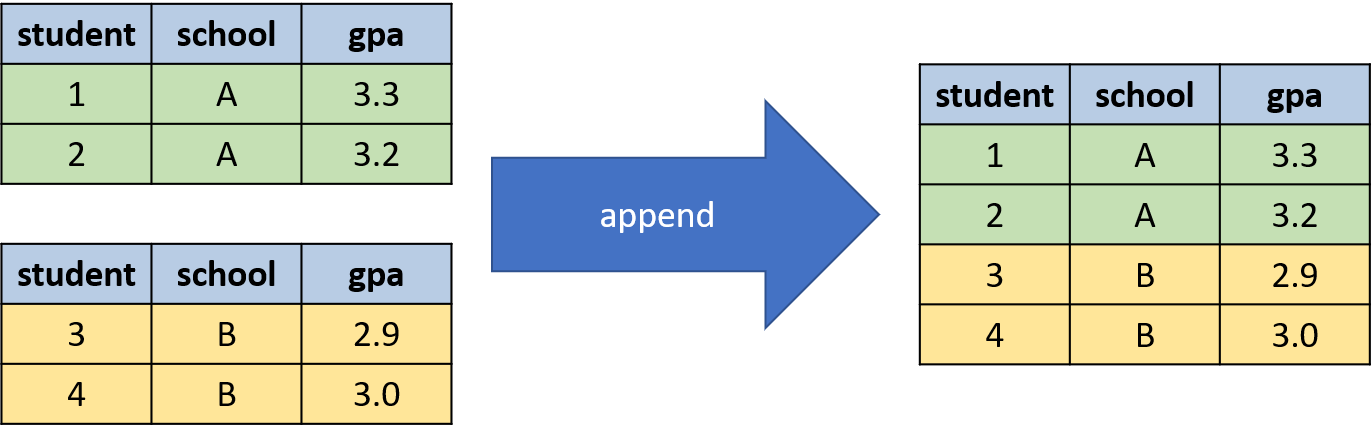
\includegraphics[width=0.6\linewidth]{images/03_append} 

}

\caption{Hypothetical Data We Want to Append Together}\label{fig:appendhyp}
\end{figure}

In this example, we have two classes: A and B, each with two students. In each dataset, we have the same variables. Our goal with \texttt{append} is to create a new dataset with 4 observations, 2 for each school.

How do we accomplish this in Stata? If class A data is stored in \texttt{classA.dta} and class B data is stored in \texttt{classB.dta} we can combine them by typing:

\begin{Shaded}
\begin{Highlighting}[]
\KeywordTok{use}\NormalTok{ classA.dta, }\KeywordTok{clear} 
\KeywordTok{append} \KeywordTok{using}\NormalTok{ classB.dta }
\end{Highlighting}
\end{Shaded}

What we have done is first load in the class A data by typing \texttt{use\ classA.dta,\ clear}. Then we have appended the class B data by typing \texttt{append\ using\ classB.dta}. For this code to work, both \texttt{classA.dta} and \texttt{classB.dta} need to be in the working directory. Additionally, the variable names in both classA and classB need to be the same. For example, if one of the datasets had the student id variable named \texttt{sid}, then you would need to make the names consistent across datasets before merging. You can rename a variable with the \texttt{rename} command. For example, to rename a variable \texttt{sid} to \texttt{student} you would type \texttt{rename\ sid\ student}.

In this example, we had two datasets to combine. Imagine we had more, for example, class C, class D and so on. You can continue to \texttt{append} more datasets by typing, for example, \texttt{append\ using\ classC.dta} followed by \texttt{append\ using\ classD.dta} and so on.

\section{Merge Basics}\label{merge-basics}

The \texttt{merge} command is used when you want to \textbf{add columns} to a dataset. For example, we are often interested in relationships between different variables. But if the variables are not in the same dataset, we need a way to combine datasets. A lot of cutting-edge research in social sciences stems from merging together previously unlinked datasets to observe new relationships.

Whenever you merge two datasets in Stata, you need to identify two things. First, what variable can the data merged on? For example, if you have two individual-level datasets, you need a unique identifier to merge individuals. If you were trying to merge two datasets on students, then a unique student identifier would be a good option. Before merging, you need to identify this variable to merge on and verify it is stored in the same format in both datasets. In many cases, there are many ways to hold the same information. For example, if you are matching two datasets at the state level, the information could be stored as abbreviations (e.g.~CA), full state name (e.g.~California), or a numeric state code (e.g.~the value 6 is equal to California for the Federal Information Processing System: FIPS). To merge datasets the information in both datasets must be stored in the same way.

The second task is to identify the type of merge. There are three types of merges in Stata: one-to-one, many-to-one and one-to-many. To understand the differences between these types of merges we will go through a few simple examples. Let's first go through a one-to-one merge, which is depicted in Figure \ref{fig:merge1to1}.

\begin{figure}

{\centering 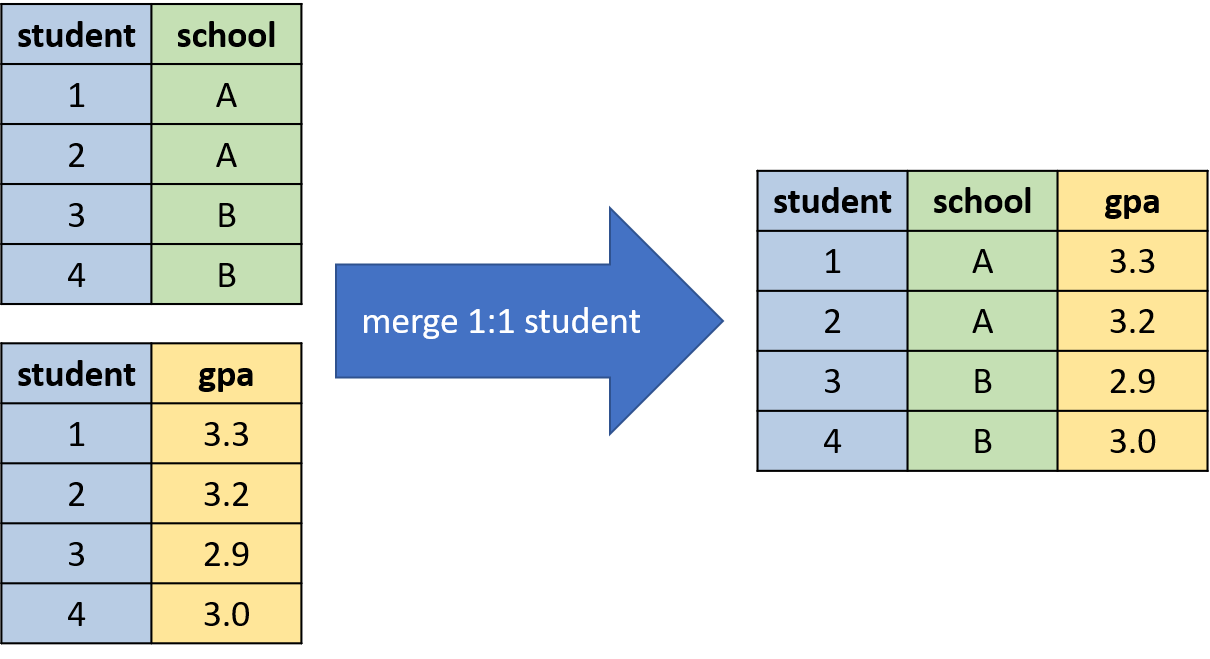
\includegraphics[width=0.6\linewidth]{images/03_merge_one} 

}

\caption{Example of a one-to-one Merge}\label{fig:merge1to1}
\end{figure}

In each dataset, there is a unique value for \texttt{student} for every observation. This is referred to as a one-to-one merge because we are matching each student in the school dataset to a single student in the gpa dataset.

A many-to-one merge or one-to-many merge is when the variable that is being merged on has multiple observations for some values in one of the two datasets. For example, in Figure \ref{fig:mergemto1}, we are merging the two datasets based on the variable \texttt{school.} But in the student-level dataset, there are multiple observations per school. In particular, students 1 and 2 attend school A, while students 3 and 4 attend school B. In the school-level dataset, there is a single observation per school.

\begin{figure}

{\centering 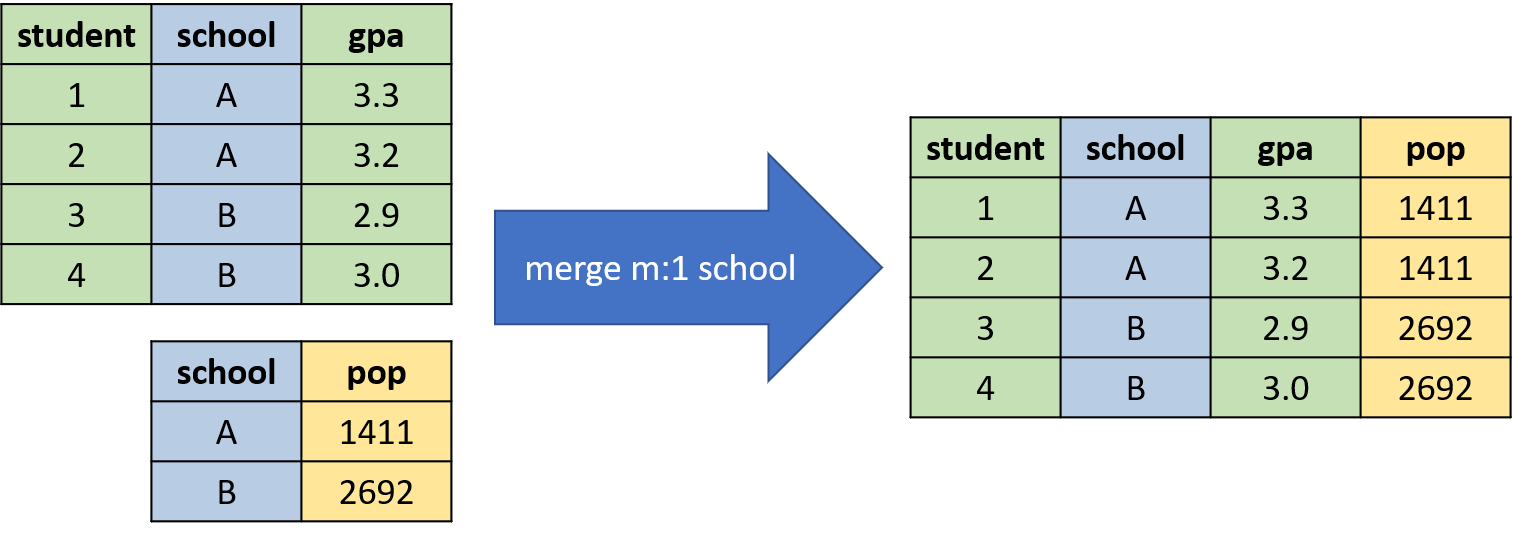
\includegraphics[width=0.6\linewidth]{images/03_merge_many} 

}

\caption{Example of a many-to-one Merge}\label{fig:mergemto1}
\end{figure}

Whether a merge is many-to-one or one-to-many depends on the order you load the datasets. But at a conceptual level, these two types of merges are the same. To understand this more clearly, we are now going to learn how to merge datasets in Stata. We will begin with a simple one-to-one merge, before proceeding to the many-to-one or one-to-many merge.

To merge two datasets in Stata, the process takes a few steps. First, you must load one of the two datasets into memory. Whichever dataset you load first is referred to as the \textbf{master dataset}. Next, you use the \texttt{merge} command to combine the master dataset with the second of the two datasets. The dataset you are merging to is called the \textbf{using dataset}.

Let's try this out on a few simple datasets. Imagine we have the two datasets below (\texttt{school.dta} and \texttt{gpa.dta}) and we want to combine them.

\begin{figure}

{\centering 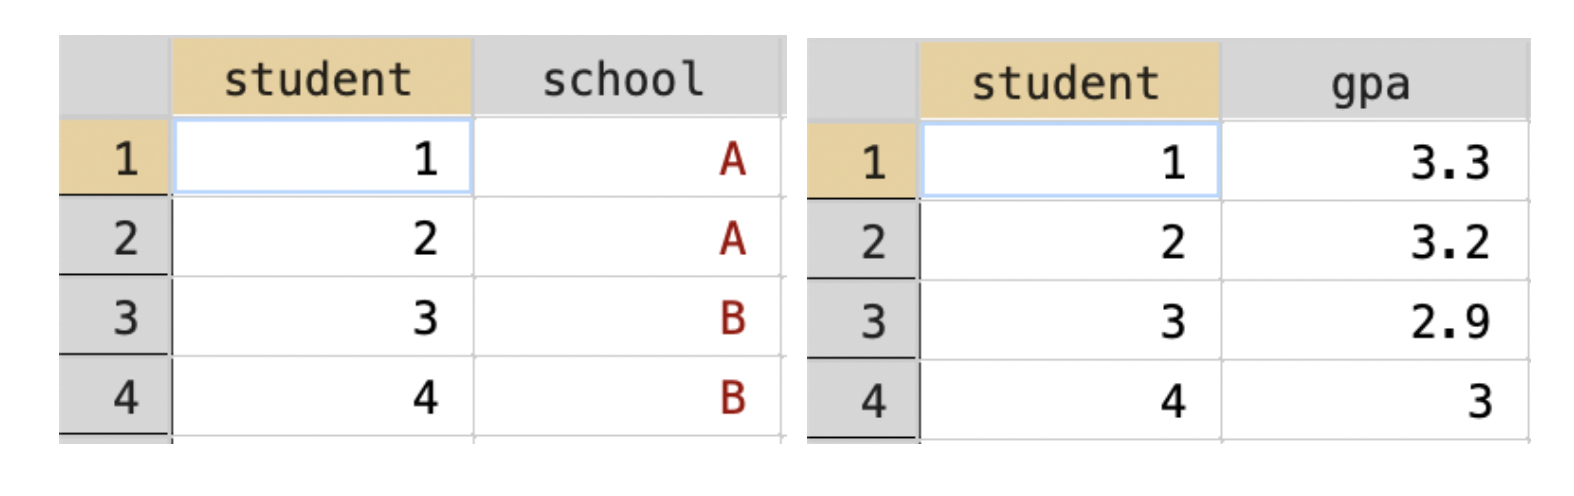
\includegraphics[width=0.6\linewidth]{images/03_merge1to1} 

}

\caption{Merging Student-Level Datasets}\label{fig:merge1to1stata}
\end{figure}

The first step is to load one of the two datasets.

\begin{Shaded}
\begin{Highlighting}[]
\KeywordTok{use}\NormalTok{ school.dta, }\KeywordTok{clear} 
\end{Highlighting}
\end{Shaded}

Because we loaded \texttt{school.dta} first, \texttt{school.dta} is the master dataset. We will now merge it to \texttt{gpa.dta}.

\begin{Shaded}
\begin{Highlighting}[]
\KeywordTok{merge}\NormalTok{ 1:1 student }\KeywordTok{using}\NormalTok{ gpa.dta}
\end{Highlighting}
\end{Shaded}

When using the \texttt{merge} command we always need to make sure of a few components. First, we have specified \texttt{student} is the variable we will merge on. Therefore, each student in \texttt{school.dta} will be matched to the corresponding student in \texttt{gpa.dta}. Second, we have specified \texttt{1:1} because each student is a unique observation in both datasets. Lastly, we have specified that we are merging to \texttt{gpa.dta} by specifying \texttt{using\ gpa.dta}.

Now let's try a many-to-one merge. Imagine we have the two datasets below (\texttt{school.dta} and \texttt{pop.dta}) and we want to combine them.

\begin{figure}

{\centering 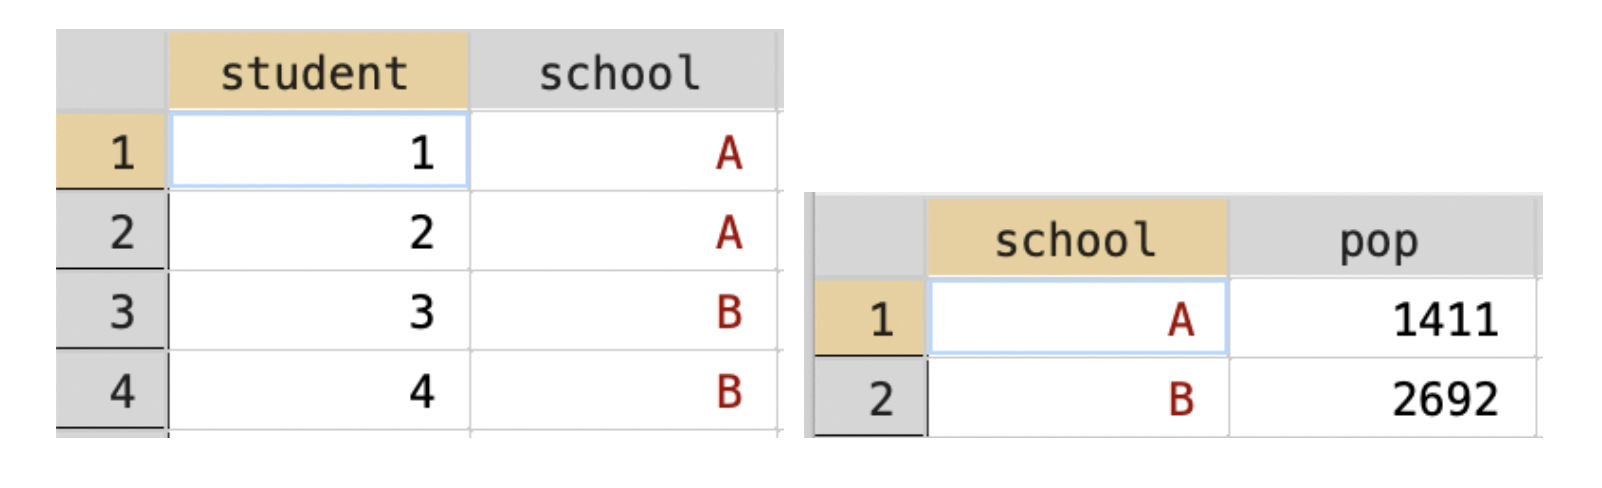
\includegraphics[width=0.6\linewidth]{images/03_mergemto1} 

}

\caption{Merging Student-Level Dataset to School-level Dataset}\label{fig:mergemto1stata}
\end{figure}

There are two main differences here. First, we will now be merging on the variable \texttt{school}, as that is the variable that is common between both the datasets. Second, in the \texttt{school.dta}dataset, there are multiple observations for each school. In the \texttt{pop.dta}, there is a single observation per school. Therefore this will be a many-to-one merge instead of a one-to-one merge. Therefore, the code to merge the two datasets is now:

\begin{Shaded}
\begin{Highlighting}[]
\KeywordTok{use}\NormalTok{ school.dta, }\KeywordTok{clear}
\KeywordTok{merge} \FunctionTok{m}\NormalTok{:1 school }\KeywordTok{using}\NormalTok{ pop.dta}
\end{Highlighting}
\end{Shaded}

We specify \texttt{m:1} because there are multiple observations per school in the master dataset, and a single in the using. A one-to-many merge (\texttt{1:m}) is conceptually similar. If we had loaded \texttt{pop.dta} first, then \texttt{pop.dta} would be the master dataset. In this case, the code to merge the two datasets is given by

\begin{Shaded}
\begin{Highlighting}[]
\KeywordTok{use}\NormalTok{ pop.dta, }\KeywordTok{clear}
\KeywordTok{merge}\NormalTok{ 1:}\FunctionTok{m}\NormalTok{ school }\KeywordTok{using}\NormalTok{ school.dta}
\end{Highlighting}
\end{Shaded}

The reason we switched to \texttt{1:m} is because there is a single observation per school in the master dataset and multiple in the using dataset now that \texttt{pop.dta} is the master dataset and \texttt{school.dta} is the using dataset. Therefore, a one-to-many merge vs.~a many-to-one merge is entirely dependent on which dataset you load first.

There is also an option to perform a many-to-many merge \texttt{m:m}, however, \textbf{you should not use this option}. Your data will be transformed in ways that you probably did not intend. The usual solution to this problem is to transform your data in a way so that you can perform a one-to-many or many-to-one merge instead

\section{Merge Advanced}\label{merge-advanced}

Sometimes, two datasets won't merge completely. For example, consider the two datasets in Figure \ref{fig:impmerge}.

\begin{figure}

{\centering 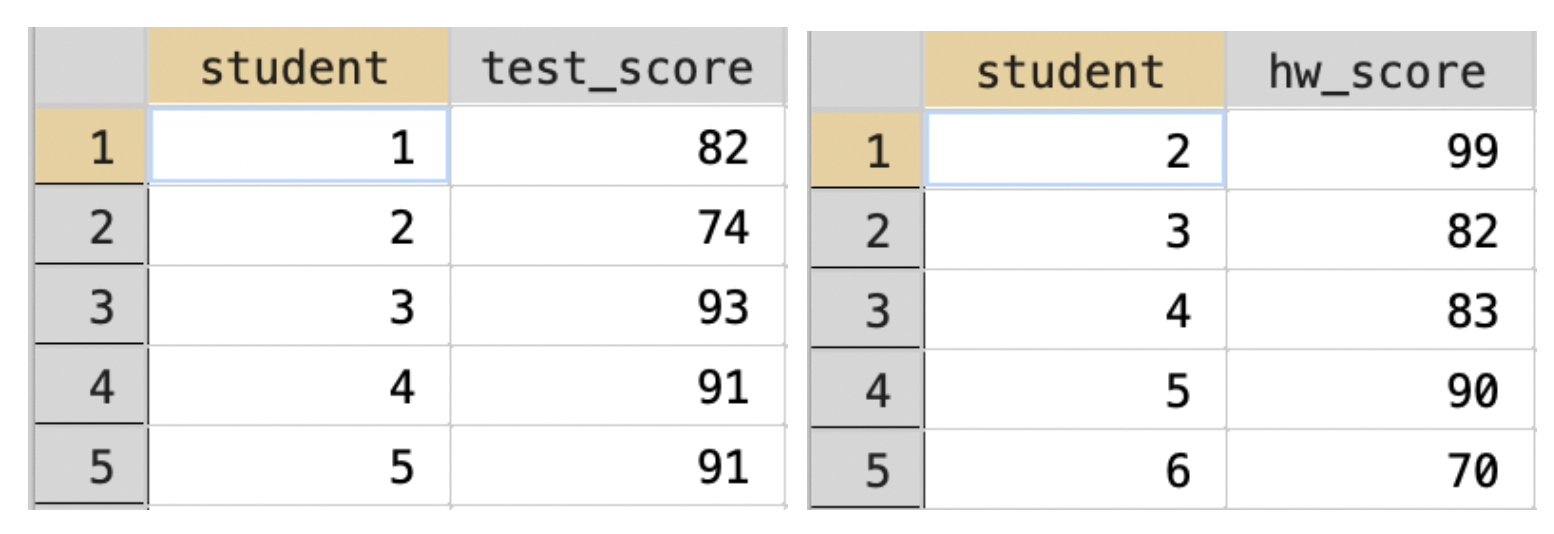
\includegraphics[width=0.6\linewidth]{images/03_imp_merge} 

}

\caption{Example of Merge with Unmatched Observations}\label{fig:impmerge}
\end{figure}

In this example, student 1 has a test score, but no homework score, while student 6 has a homework score but no test score. Let's see what happens if we merge these two datasets in Stata.

\begin{Shaded}
\begin{Highlighting}[]
\CommentTok{/* change working directory */}
\NormalTok{cd /Users/davidarnold/Dropbox/Teaching/EP5/online/03\_week/}\KeywordTok{data}
\NormalTok{file gapminder.dta }\KeywordTok{not}\NormalTok{ Stata }\KeywordTok{format}
\FunctionTok{r}\NormalTok{(610);}


\NormalTok{/Users/davidarnold/Dropbox/Teaching/EP5/online/03\_week/}\KeywordTok{data}
\end{Highlighting}
\end{Shaded}

\begin{Shaded}
\begin{Highlighting}[]
\CommentTok{/*load test score data*/}
\KeywordTok{use}\NormalTok{ test\_score.dta, }\KeywordTok{clear} 

\CommentTok{/*merge to the hw data*/}
\KeywordTok{merge}\NormalTok{ 1:1 student }\KeywordTok{using}\NormalTok{ hw\_score.dta}
\NormalTok{file gapminder.dta }\KeywordTok{not}\NormalTok{ Stata }\KeywordTok{format}
\FunctionTok{r}\NormalTok{(610);}


\NormalTok{file test\_score.dta }\KeywordTok{not}\NormalTok{ found}
\FunctionTok{r}\NormalTok{(601);}

\FunctionTok{r}\NormalTok{(601);}
\end{Highlighting}
\end{Shaded}

Two observations were not matched. One from the master dataset (\texttt{test\_score.dta}) and the other from the using dataset (\texttt{hw\_score.dta}). A new variable (named \texttt{\_merge}) has been added to the dataset to keep track of matched vs.~unmatched observations. It is equal to 1 for observations only in the master dataset, 2 for observations only in the using, and 3 for observations in both the master and the using dataset.

Whether you keep unmatched observations in your dataset depends a bit on your analysis. If you really need both homework score and test score for all of your analysis, you can probably safely keep only matched observations. To do this in Stata after a \texttt{merge} command, we can type

\begin{Shaded}
\begin{Highlighting}[]
\KeywordTok{keep} \KeywordTok{if} \DataTypeTok{\_merge}\NormalTok{==3}
\NormalTok{file gapminder.dta }\KeywordTok{not}\NormalTok{ Stata }\KeywordTok{format}
\FunctionTok{r}\NormalTok{(610);}


\DataTypeTok{\_merge} \KeywordTok{not}\NormalTok{ found}
\FunctionTok{r}\NormalTok{(111);}

\FunctionTok{r}\NormalTok{(111);}
\end{Highlighting}
\end{Shaded}

You can also specify to only keep matched observations directly in the merge command. If you are only keeping observations that match between the two datasets, you don't need to generate the \texttt{\_merge} variable, as it will be equal to 3 for all matched observations. Instead, you can specify the option \texttt{keep(3)} which only keeps matched observations. Then, to prevent Stata from adding an uniformative variable \texttt{\_merge}, you can also specify \texttt{nogen} so that the variable is not generated. The example below uses both these options in the context of our hypothetical example.

\begin{Shaded}
\begin{Highlighting}[]
\KeywordTok{use}\NormalTok{ test\_score.dta, }\KeywordTok{clear} 
\KeywordTok{merge}\NormalTok{ 1:1 student }\KeywordTok{using}\NormalTok{ hw\_score.dta, }\KeywordTok{keep}\NormalTok{(3) nogen}
\NormalTok{file gapminder.dta }\KeywordTok{not}\NormalTok{ Stata }\KeywordTok{format}
\FunctionTok{r}\NormalTok{(610);}


\NormalTok{file test\_score.dta }\KeywordTok{not}\NormalTok{ found}
\FunctionTok{r}\NormalTok{(601);}

\FunctionTok{r}\NormalTok{(601);}
\end{Highlighting}
\end{Shaded}

As you can see, the generated table has only 4 observations now, all of which are in both datasets. This is because we have specified to only keep observations that are in both datasets by specifying \texttt{keep(3)}.

Now that we understand how to use the \texttt{merge} command, let's go through a few common mistakes. The first has to deal with the matching variable. The matching variables need to be named in the exact same way.

In the example below (Figure \ref{fig:samename}), the two datasets are the same as the previous example, but the student variable is named \texttt{student\_id} in one and \texttt{student} in the other

\begin{figure}

{\centering 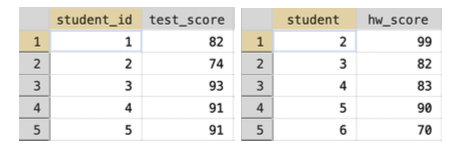
\includegraphics[width=0.6\linewidth]{images/03_samename} 

}

\caption{Example of Merge with Different Names for Matching Variables}\label{fig:samename}
\end{figure}

Let's see what happens if we try to merge these two together:

\begin{Shaded}
\begin{Highlighting}[]
\KeywordTok{use}\NormalTok{ test\_score2.dta, }\KeywordTok{clear} 
\KeywordTok{merge}\NormalTok{ 1:1 student\_id }\KeywordTok{using}\NormalTok{ hw\_score.dta}
\NormalTok{file gapminder.dta }\KeywordTok{not}\NormalTok{ Stata }\KeywordTok{format}
\FunctionTok{r}\NormalTok{(610);}


\NormalTok{file test\_score2.dta }\KeywordTok{not}\NormalTok{ found}
\FunctionTok{r}\NormalTok{(601);}

\FunctionTok{r}\NormalTok{(601);}
\end{Highlighting}
\end{Shaded}

The variable \texttt{student\_id} was not found because the variable \texttt{student\_id} does not exist in the using dataset. To merge these two datasets together properly, we need to make sure the names of the variables are the same. If they are not, you can use the \texttt{rename} command to ensure the names are the same.

Similarly, matching variables must be the same type of variable. For example, in Figure \ref{fig:sametype}, the student variable is stored as a string in the first dataset (which is why it is highlighted in red), while it is stored as a numeric variable in the second dataset (which is why it is highlighted in black).

\begin{figure}

{\centering 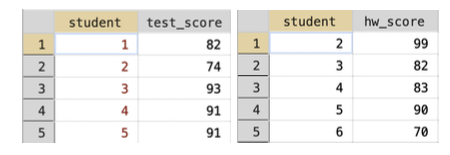
\includegraphics[width=0.6\linewidth]{images/03_sameformat} 

}

\caption{Example of Merge with Different Types for Matching Variable}\label{fig:sametype}
\end{figure}

Let's see what happens if we try to merge these two together

\begin{Shaded}
\begin{Highlighting}[]
\KeywordTok{use}\NormalTok{ test\_score3.dta, }\KeywordTok{clear} 
\KeywordTok{merge}\NormalTok{ 1:1 student }\KeywordTok{using}\NormalTok{ hw\_score.dta}
\NormalTok{file gapminder.dta }\KeywordTok{not}\NormalTok{ Stata }\KeywordTok{format}
\FunctionTok{r}\NormalTok{(610);}


\NormalTok{file test\_score3.dta }\KeywordTok{not}\NormalTok{ found}
\FunctionTok{r}\NormalTok{(601);}

\FunctionTok{r}\NormalTok{(601);}
\end{Highlighting}
\end{Shaded}

This error code is describing how the format of the variables is different in our master vs.~using dataset. To fix this issue, we need to convert one of the variable formats. For example, we could type \texttt{destring\ student,\ replace} to convert the student variable to a numeric variable in the \texttt{test\_score3.dta} dataset.

Lastly, we have discussed one-to-one merges, many-to-one merges and one-to-many merges, but what about many-to-many merges? The reason we have not discussed it is because \textbf{you should never do many-to-many merges in Stata}. In most cases, the right way to proceed if you find yourself faced with a many-to-many merge is to restructure your data. Usually you can use some data wrangling (like \texttt{collapse}) to transform your data into a one-to-one, many-to-one or one-to-many merge. There is a command \texttt{joinby} that does accomplish something like a many-to-many merge, but we will not discuss this command in this book.

\section{Build Data}\label{build-data}

Now that we understand the merge command, let's use it to merge traffic stop data to data on sunset times so that we can implement the veil of darkness test. To begin, we need to choose a period of time in San Diego in which it is sometimes light and sometimes dark, depending on the time of the year. Let's choose the time period 6:30-7:00 PM. Sometimes it is dark out at 6:30-7:00 PM (in winter for example), while sometimes it is light out (in summer for example). We need to identify whether it was light or dark for every stop in our data.

The problem, however, is that our data for stops currently comes in two separate files, one for the years 2014-2015 and one for the years 2016-2017. Additionally, our sunset data comes in a separate file. Therefore, we have three separate files that we need to combine to create one final dataset.

To create a dataset of all stops between 2014-2017, we need to \texttt{append} the stop-level data.

\begin{Shaded}
\begin{Highlighting}[]
\KeywordTok{use}\NormalTok{ san\_diego\_stops\_2014\_2015.dta, }\KeywordTok{clear}
\KeywordTok{append} \KeywordTok{using}\NormalTok{ san\_diego\_stops\_2016\_2017.dta}
\NormalTok{file gapminder.dta }\KeywordTok{not}\NormalTok{ Stata }\KeywordTok{format}
\FunctionTok{r}\NormalTok{(610);}


\NormalTok{file san\_diego\_stops\_2014\_2015.dta }\KeywordTok{not}\NormalTok{ found}
\FunctionTok{r}\NormalTok{(601);}

\FunctionTok{r}\NormalTok{(601);}
\end{Highlighting}
\end{Shaded}

So it might look as if nothing happened in Stata. To check that we now have all years of data in a single dataset we can type:

\begin{Shaded}
\begin{Highlighting}[]
\KeywordTok{tab} \FunctionTok{year}
\end{Highlighting}
\end{Shaded}

\begin{verbatim}
file gapminder.dta not Stata format
r(610);


no variables defined
r(111);

r(111);
\end{verbatim}

Now we have verified that the current data in memory has stops between 2014-2017. Our next task is to \texttt{merge} in the data on sunset times. To do this, we need to make sure of two things. First, is there a variable that we can merge on? In general, you would need to load both datasets and check if there are any variables that store the same information. In our case, there is a single variable that meets this criteria: \texttt{date}. Second, is this a one-to-one or many-to-one merge? Third, is the \texttt{date} variable in both datasets stored in the same format?

To get started, we need to figure out how many observations there are for a given \texttt{date} in each dataset. Intuitively, we expect there are multiple observations per \texttt{date} in the traffic stop data. In other words, officers stop more than one individual per day. In the sunset data, well there is only a single sunset time for every day, so we expect a single observation per \texttt{date}. But data is not always stored how we expect, so it is always good to check this. The way were are going to check is through the \texttt{unique} command.

The \texttt{unique} command does not come installed in Stata. You need to install it into your version of Stata by typing \texttt{ssc\ install\ unique} into the Command window. In general, you might find a command online that will help you perform some data analysis. Many commands can be installed by typing \texttt{ssc\ install\ commandname}. Therefore, before running the line of code below, you should type \texttt{ssc\ install\ unique} into the Command window and press enter.

\begin{Shaded}
\begin{Highlighting}[]
\KeywordTok{unique} \FunctionTok{date}
\end{Highlighting}
\end{Shaded}

\begin{verbatim}
file gapminder.dta not Stata format
r(610);


variable date not found
r(111);

r(111);
\end{verbatim}

How do we interpret this output? Well, the number of unique values of date is 1186. In other words, this is how many different days there are in our dataset on traffic stops. In contrast, there are 381,149 total stops. Therefore, there are multiple stops per day. Whenever you see more records than unique values, you know this is a \texttt{many-to-BLANK} merge. The next job for us is to figure out if the \texttt{BLANK} should be replaced by a \texttt{one}. To do this we need to load the \texttt{sd\_sunset.dta}.

\begin{Shaded}
\begin{Highlighting}[]
\KeywordTok{use}\NormalTok{ sd\_sunset.dta, }\KeywordTok{clear}
\NormalTok{file gapminder.dta }\KeywordTok{not}\NormalTok{ Stata }\KeywordTok{format}
\FunctionTok{r}\NormalTok{(610);}


\NormalTok{file sd\_sunset.dta }\KeywordTok{not}\NormalTok{ found}
\FunctionTok{r}\NormalTok{(601);}

\FunctionTok{r}\NormalTok{(601);}
\end{Highlighting}
\end{Shaded}

\begin{Shaded}
\begin{Highlighting}[]
\KeywordTok{unique} \FunctionTok{date}
\end{Highlighting}
\end{Shaded}

\begin{verbatim}
file gapminder.dta not Stata format
r(610);


variable date not found
r(111);

r(111);
\end{verbatim}

In this dataset, there are 1186 unique values of date and 1186 records. Each value of date is a unique observation in the dataset. Therefore, we can conclude that this is a \texttt{many-to-one} merge. There are many observations per value of \texttt{date} in the stops data, but one observation per value of \texttt{date} in the sunset data.

The last thing we need to do is to check that the format of the date variable is the same in both datasets. Let's look at the first observation in the \texttt{sd\_sunset.dta}

\begin{Shaded}
\begin{Highlighting}[]
\OtherTok{list} \FunctionTok{date} \KeywordTok{if} \DataTypeTok{\_n}\NormalTok{==1}
\NormalTok{file gapminder.dta }\KeywordTok{not}\NormalTok{ Stata }\KeywordTok{format}
\FunctionTok{r}\NormalTok{(610);}


\NormalTok{no variables defined}
\FunctionTok{r}\NormalTok{(111);}

\FunctionTok{r}\NormalTok{(111);}
\end{Highlighting}
\end{Shaded}

Now, let's go back to the stop-level data and check if \texttt{date} is held in the same format.

\begin{Shaded}
\begin{Highlighting}[]
\KeywordTok{use}\NormalTok{ san\_diego\_stops\_2014\_2015.dta, }\KeywordTok{clear}
\KeywordTok{append} \KeywordTok{using}\NormalTok{ san\_diego\_stops\_2016\_2017.dta}
\NormalTok{file gapminder.dta }\KeywordTok{not}\NormalTok{ Stata }\KeywordTok{format}
\FunctionTok{r}\NormalTok{(610);}


\NormalTok{file san\_diego\_stops\_2014\_2015.dta }\KeywordTok{not}\NormalTok{ found}
\FunctionTok{r}\NormalTok{(601);}

\FunctionTok{r}\NormalTok{(601);}
\end{Highlighting}
\end{Shaded}

\begin{Shaded}
\begin{Highlighting}[]
\OtherTok{list} \FunctionTok{date} \KeywordTok{if} \DataTypeTok{\_n}\NormalTok{==1}
\NormalTok{file gapminder.dta }\KeywordTok{not}\NormalTok{ Stata }\KeywordTok{format}
\FunctionTok{r}\NormalTok{(610);}


\NormalTok{no variables defined}
\FunctionTok{r}\NormalTok{(111);}

\FunctionTok{r}\NormalTok{(111);}
\end{Highlighting}
\end{Shaded}

It looks like the \texttt{date} variable is in the same format. If it is not, you then will need to do some data wrangling in order to get it into the same format. For us, we can now merge this data to the sunset data:

\begin{Shaded}
\begin{Highlighting}[]
\KeywordTok{merge} \FunctionTok{m}\NormalTok{:1 }\FunctionTok{date} \KeywordTok{using}\NormalTok{ sd\_sunset.dta, }\KeywordTok{keep}\NormalTok{(3) nogen}
\end{Highlighting}
\end{Shaded}

\begin{verbatim}
file gapminder.dta not Stata format
r(610);


no variables defined
r(111);

r(111);
\end{verbatim}

Because we specified \texttt{keep(3)\ nogen}, we are only keeping observations that correspond to dates in both datasets. Now, we are going to want to use this data for our analysis later, so let's save the combined dataset under a new name: \texttt{sd\_analysis\_sample.dta} by typing:

\begin{Shaded}
\begin{Highlighting}[]
\KeywordTok{save}\NormalTok{ sd\_analysis\_sample.dta, }\KeywordTok{replace} 
\end{Highlighting}
\end{Shaded}

This code will place a new file in your working directory named \texttt{sd\_analysis\_sample.dta}. Next time you want to work with your data, you can now load this file directly, and won't need to repeat the steps of appending and merging datasets together.

\section{Date-Time}\label{date-time}

Now that we have all the information to perform the veil of darkness test, we need to restrict to stops for which the test applies. To remind you, we will explore whether the composition of traffic stops by race varies by whether it is light or dark out, controlling for the time of the stop.

In order to do this, we will restrict to traffic stops that occur between 6:30-7:00 PM. In San Diego, in parts of the year, it is dark out at 6:30-7:00 PM. At other times it is light out. This is, of course, not the only time slot that will work. In fact, the methods in Grogger and Ridgeway (2006) use all such times that are sometimes light and sometimes dark. Performing this analysis requires statistical techniques beyond the level of this class, so we will instead focus on one particular block of time: 6:30-7:00 PM.

So we need to restrict to all stops that occur in this time period. Doing this will be harder than you think! We need to learn how Stata stores the time of the day.

In Stata, times of the day are often held in terms of milliseconds from midnight. Why? Well, you could store it as a string variable, but you can't add string variables. For example, while I understand that the string \texttt{"6:00\ PM"} is equal to 6:00 PM at night, I need a way to store the information so that I can do things like add or subtract additional time (i.e.~if I add an hour to 6:00 PM the result should be 7:00 PM). Strings are interpreted as words in Stata and so cannot be added in this way.

To see how Stata stores times, we can \texttt{summarize} our variable \texttt{stop\_time}.

\begin{Shaded}
\begin{Highlighting}[]
  \KeywordTok{use}\NormalTok{ sd\_analysis\_sample.dta, }\KeywordTok{replace}
\NormalTok{file gapminder.dta }\KeywordTok{not}\NormalTok{ Stata }\KeywordTok{format}
\FunctionTok{r}\NormalTok{(610);}


\NormalTok{file sd\_analysis\_sample.dta }\KeywordTok{not}\NormalTok{ found}
\FunctionTok{r}\NormalTok{(601);}

\FunctionTok{r}\NormalTok{(601);}
\end{Highlighting}
\end{Shaded}

\begin{Shaded}
\begin{Highlighting}[]
  \KeywordTok{sum}\NormalTok{ stop\_time }
\end{Highlighting}
\end{Shaded}

\begin{verbatim}
file gapminder.dta not Stata format
r(610);


no variables defined
r(111);

r(111);
\end{verbatim}

It is stored in terms of milliseconds from midnight (so 0 is midnight exactly and 1 hour later (1:00 AM) would be \(60\cdot 60 \cdot 1000 = 3,600,000\), because there are 60 minutes in an hour, 60 seconds in a minute, and a 1000 milliseconds in a second). So how many milliseconds to 6:30 PM?

\[
\underbrace{18}_{\text{hours}} \cdot \underbrace{3,600,000}_{\text{ms per hour}} + \underbrace{1,800,000}_{\text{ms per half hour}}=66,600,000
\]
So if we are restricting to 6:30 PM to 7:00 PM, we should restrict to all stops with values of \texttt{stop\_time} between 66,600,000 (6:30 PM) and 68,400,000 (7:00 PM).

While this procedure will get you the right answer, typing some large numbers can sometimes lead to transcription errors if you are not careful. A better way to do this is to use Stata commands that do this math for you. The \texttt{clock()} command automatically translates time as we usually interpret it (i.e.~9:00 AM) into milliseconds from midnight automatically.

For example, to see how many milliseconds there are from midnight to 6:00 PM, we can type:

\begin{Shaded}
\begin{Highlighting}[]
  \KeywordTok{di}\NormalTok{ clock(}\StringTok{"18:30:00"}\NormalTok{,}\StringTok{"hms"}\NormalTok{)}
\NormalTok{file gapminder.dta }\KeywordTok{not}\NormalTok{ Stata }\KeywordTok{format}
\FunctionTok{r}\NormalTok{(610);}


\NormalTok{66600000}
\end{Highlighting}
\end{Shaded}

Where \texttt{"18:30:00"} is 6:30 PM on a 24-hour clock. \texttt{"hms"} tells Stata that time should be interpreted as hours, minutes, seconds. Now that we understand how to use the \texttt{clock} command, we can use it to restrict to stops that occurred between 6:30 PM and 7:00 PM:

\begin{Shaded}
\begin{Highlighting}[]
\CommentTok{/* drop if before 6:30 PM */}
\KeywordTok{drop} \KeywordTok{if}\NormalTok{ stop\_time\textless{}clock(}\StringTok{"18:30:00"}\NormalTok{,}\StringTok{"hms"}\NormalTok{)}
\CommentTok{/* drop if after 7:00 PM */}
\KeywordTok{drop} \KeywordTok{if}\NormalTok{ stop\_time\textgreater{}clock(}\StringTok{"19:00:00"}\NormalTok{,}\StringTok{"hms"}\NormalTok{) }
\NormalTok{file gapminder.dta }\KeywordTok{not}\NormalTok{ Stata }\KeywordTok{format}
\FunctionTok{r}\NormalTok{(610);}


\NormalTok{stop\_time }\KeywordTok{not}\NormalTok{ found}
\FunctionTok{r}\NormalTok{(111);}

\FunctionTok{r}\NormalTok{(111);}
\end{Highlighting}
\end{Shaded}

Next, we need to generate indicators that tell us whether a given stop occurred during sunlight or in the dark. We will define a traffic stop occurring in the sunlight if it occurs before sunset. The variable \texttt{sunset} in the data contains the time of the sunset, which we can compare to the \texttt{stop\_time} to generate an indicator for \texttt{light}:

\begin{Shaded}
\begin{Highlighting}[]
\KeywordTok{gen}\NormalTok{ light = (stop\_time\textless{}sunset)}
\NormalTok{file gapminder.dta }\KeywordTok{not}\NormalTok{ Stata }\KeywordTok{format}
\FunctionTok{r}\NormalTok{(610);}


\NormalTok{stop\_time }\KeywordTok{not}\NormalTok{ found}
\FunctionTok{r}\NormalTok{(111);}

\FunctionTok{r}\NormalTok{(111);}
\end{Highlighting}
\end{Shaded}

In words, we are creating a variable that is equal to 1 if the time of the stop occurred before sunset, and zero otherwise. We will define a traffic stop occurring in the dark if it occurs after dusk (dusk is about 30 minutes after sunset). The variable \texttt{dusk} in the data contains the time of dusk, which we can compare to the \texttt{stop\_time} to generate an indicator for \texttt{dark}:

\begin{Shaded}
\begin{Highlighting}[]
\KeywordTok{gen}\NormalTok{ dark = (stop\_time\textgreater{}dusk)}
\NormalTok{file gapminder.dta }\KeywordTok{not}\NormalTok{ Stata }\KeywordTok{format}
\FunctionTok{r}\NormalTok{(610);}


\NormalTok{stop\_time }\KeywordTok{not}\NormalTok{ found}
\FunctionTok{r}\NormalTok{(111);}

\FunctionTok{r}\NormalTok{(111);}
\end{Highlighting}
\end{Shaded}

Now, there are some stops that occur between sunset and dusk. For these stops, we aren't sure if driver race is observed. It is neither fully light nor fully dark at these times (i.e.~\texttt{dark==0\ \&\ light==0}). We are going to drop these stops from the analysis:

\begin{Shaded}
\begin{Highlighting}[]
\KeywordTok{drop} \KeywordTok{if}\NormalTok{ light==0 \& dark==0 }
\NormalTok{file gapminder.dta }\KeywordTok{not}\NormalTok{ Stata }\KeywordTok{format}
\FunctionTok{r}\NormalTok{(610);}


\NormalTok{light }\KeywordTok{not}\NormalTok{ found}
\FunctionTok{r}\NormalTok{(111);}

\FunctionTok{r}\NormalTok{(111);}
\end{Highlighting}
\end{Shaded}

Now we are ready to start our analysis to implement the veil of darkness.

\section{Implement VOD}\label{implement-vod}

We need to compare the composition of traffic stops in times of sunlight vs.~darkness to implement the veil of darkness test. If stop rates for minorities drop in the dark, that indicates they were being targeted in the sunlight. To retrieve the composition of traffic stops by race, we can use the \texttt{tab} command:

\begin{Shaded}
\begin{Highlighting}[]
\KeywordTok{tab}\NormalTok{ subject\_race }
\end{Highlighting}
\end{Shaded}

\begin{verbatim}
file gapminder.dta not Stata format
r(610);


no variables defined
r(111);

r(111);
\end{verbatim}

If we want the composition but restricted to stops in the sunlight, we can add a conditional statement to our code:

\begin{Shaded}
\begin{Highlighting}[]
\KeywordTok{tab}\NormalTok{ subject\_race }\KeywordTok{if}\NormalTok{ dark==0 }
\end{Highlighting}
\end{Shaded}

\begin{verbatim}
file gapminder.dta not Stata format
r(610);


no variables defined
r(111);

r(111);
\end{verbatim}

Now let's look at the composition of traffic stops in the dark:

\begin{Shaded}
\begin{Highlighting}[]
\KeywordTok{tab}\NormalTok{ subject\_race }\KeywordTok{if}\NormalTok{ dark==1 }
\end{Highlighting}
\end{Shaded}

\begin{verbatim}
file gapminder.dta not Stata format
r(610);


no variables defined
r(111);

r(111);
\end{verbatim}

In these tables, we are trying to see if certain races are much less likely to be stopped in darkness relative to sunlight. If this is true, then this is good evidence that this race is being targeted during sunlight hours. From the table above, the composition of traffic stops seems relatively similar during sunlight vs.~after dark. However, it is a little difficult to absorb all the information from these multiple tables. To really get the information across, it might be useful to put this information into a figure.

\section{Bar Graphs}\label{bar-graphs}

Eventually, we are going to use a bar graph to visualize the veil of darkness test for discrimination. In this section, we are going to learn how to construct bar graphs in Stata generally. To begin, we are going to set up a hypothetical example. Imagine we are trying to construct a bar graph that shows the average GPA across different schools, based on the data below:

\begin{figure}

{\centering 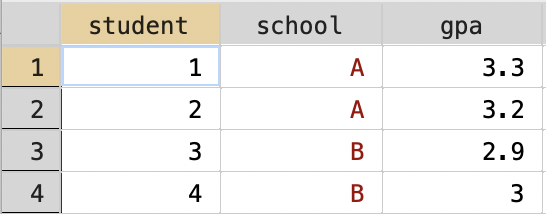
\includegraphics[width=0.65\linewidth]{images/03_school_gpa} 

}

\caption{Dataset on Schools and GPA}\label{fig:schoolgpa}
\end{figure}

The command \texttt{graph\ bar} is used to make bar graphs in Stata. There are lots of ways this command can be altered, so make sure to look at the help file! To start, we are going to create a bar graph that shows the average GPA for each school.

The basic syntax for the \texttt{graph\ bar} command is

\begin{Shaded}
\begin{Highlighting}[]
\KeywordTok{graph} \BaseNTok{bar}\NormalTok{ (stat) yvar, }\BaseNTok{over}\NormalTok{(xvar)}
\end{Highlighting}
\end{Shaded}

\texttt{(stat)} will be \texttt{(mean)} if you want the average value of the y-variable to be displayed. There are also other options in the help file. For example, you could have the command plot the count, the minimum, maximum, median, among other statistics. \texttt{over(xvar)} will be the variable that defines the groups on the horizontal axis.

In our example, we want the average of the variable \texttt{gpa}, so we will type \texttt{(mean)\ gpa}. What do want the average over? The class variable. So we will type \texttt{over(class)}. All together:

\begin{Shaded}
\begin{Highlighting}[]
\KeywordTok{graph} \BaseNTok{bar}\NormalTok{ (}\KeywordTok{mean}\NormalTok{) gpa, }\BaseNTok{over}\NormalTok{(school)}
\end{Highlighting}
\end{Shaded}

\begin{figure}

{\centering 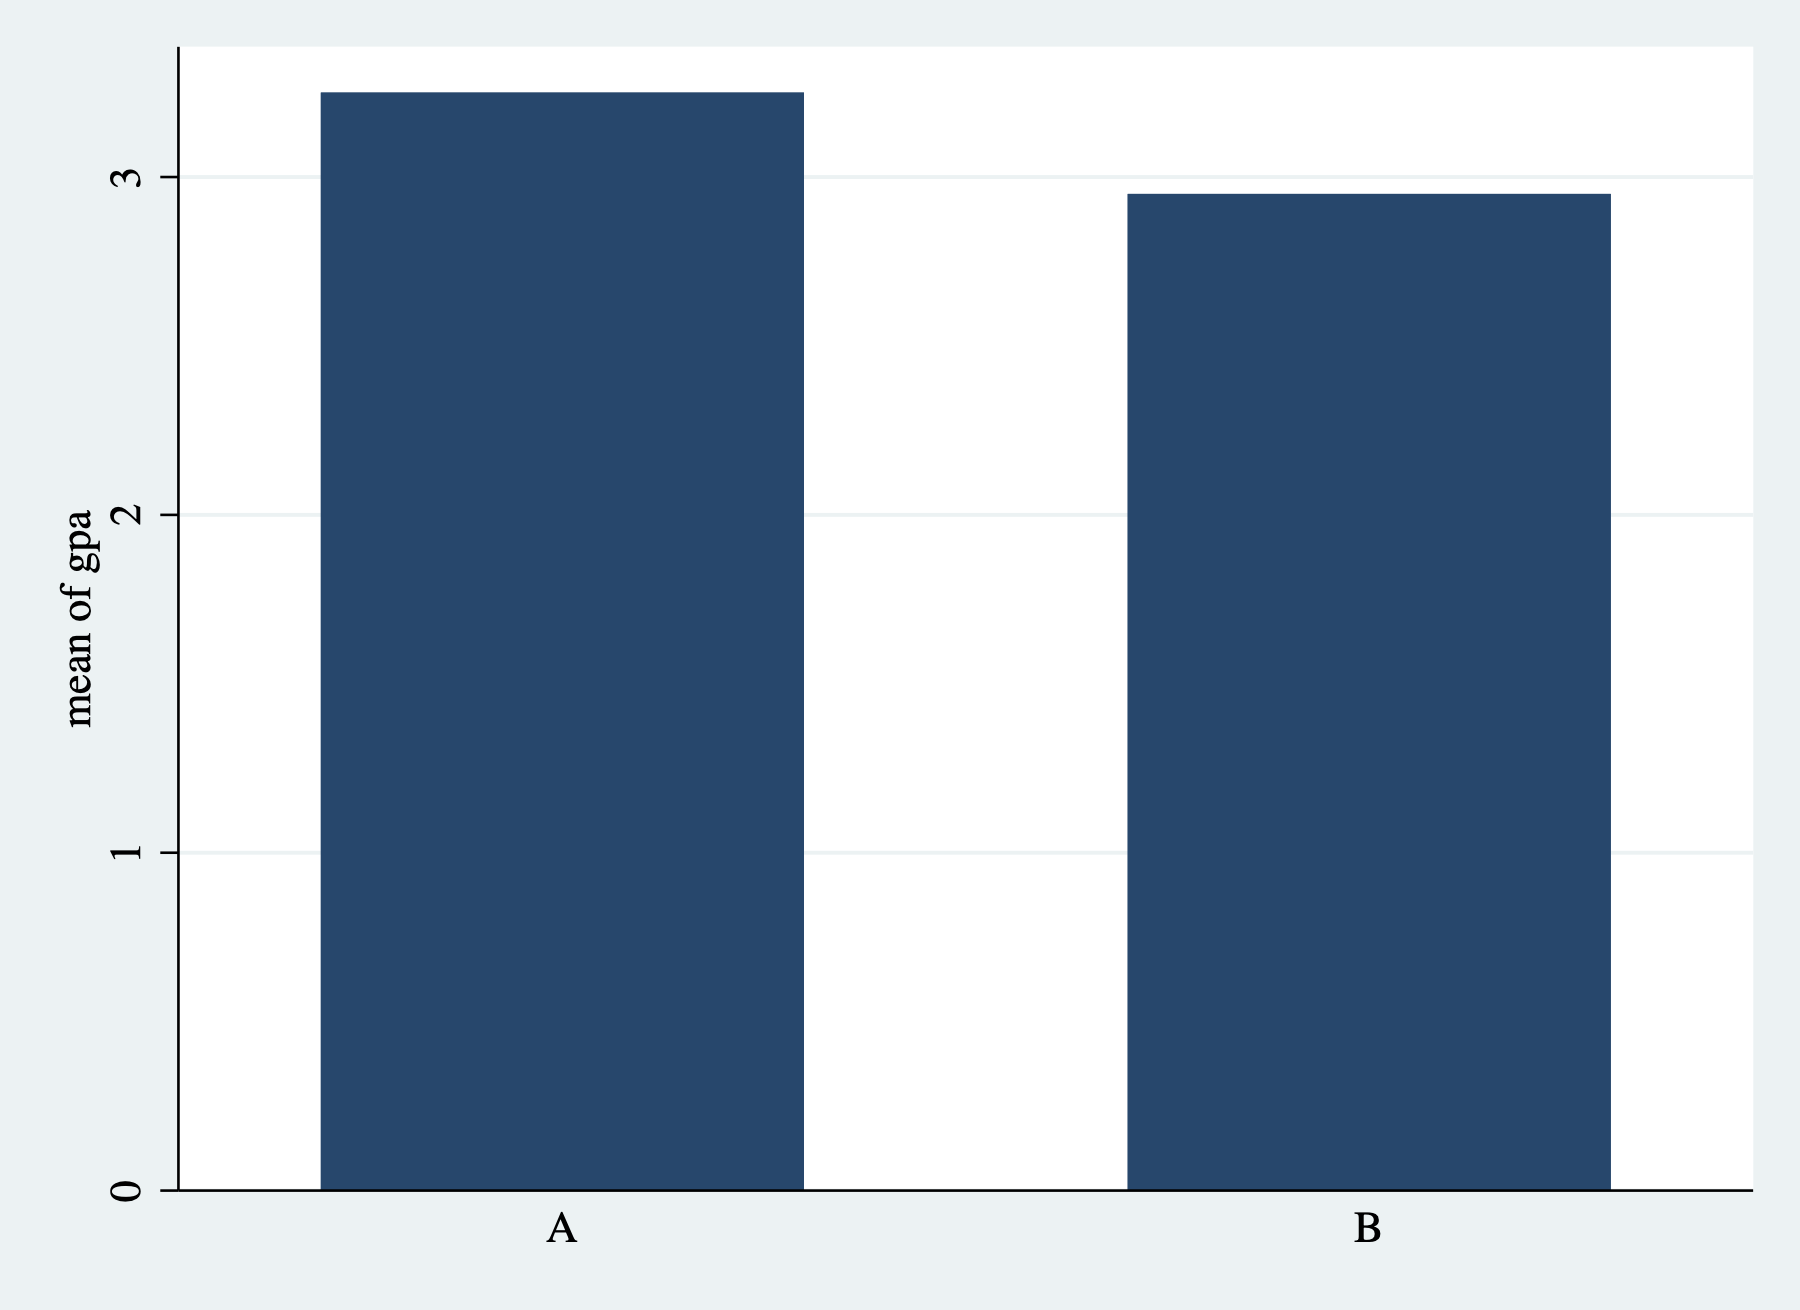
\includegraphics[width=0.65\linewidth]{images/03_bar_ex} 

}

\caption{Simple Bar Graph}\label{fig:barex}
\end{figure}

As always need descriptive titles and properly labeled axes. We can add these the same way we added them for histograms:

\begin{Shaded}
\begin{Highlighting}[]
\KeywordTok{graph} \BaseNTok{bar}\NormalTok{ (}\KeywordTok{mean}\NormalTok{) gpa, }\BaseNTok{over}\NormalTok{(school) }\CommentTok{///}
    \BaseNTok{title}\NormalTok{(}\StringTok{"Average GPA by Classroom"}\NormalTok{) }\CommentTok{///}
    \BaseNTok{ytitle}\NormalTok{(}\StringTok{"Average GPA"}\NormalTok{) }
\end{Highlighting}
\end{Shaded}

\begin{figure}

{\centering 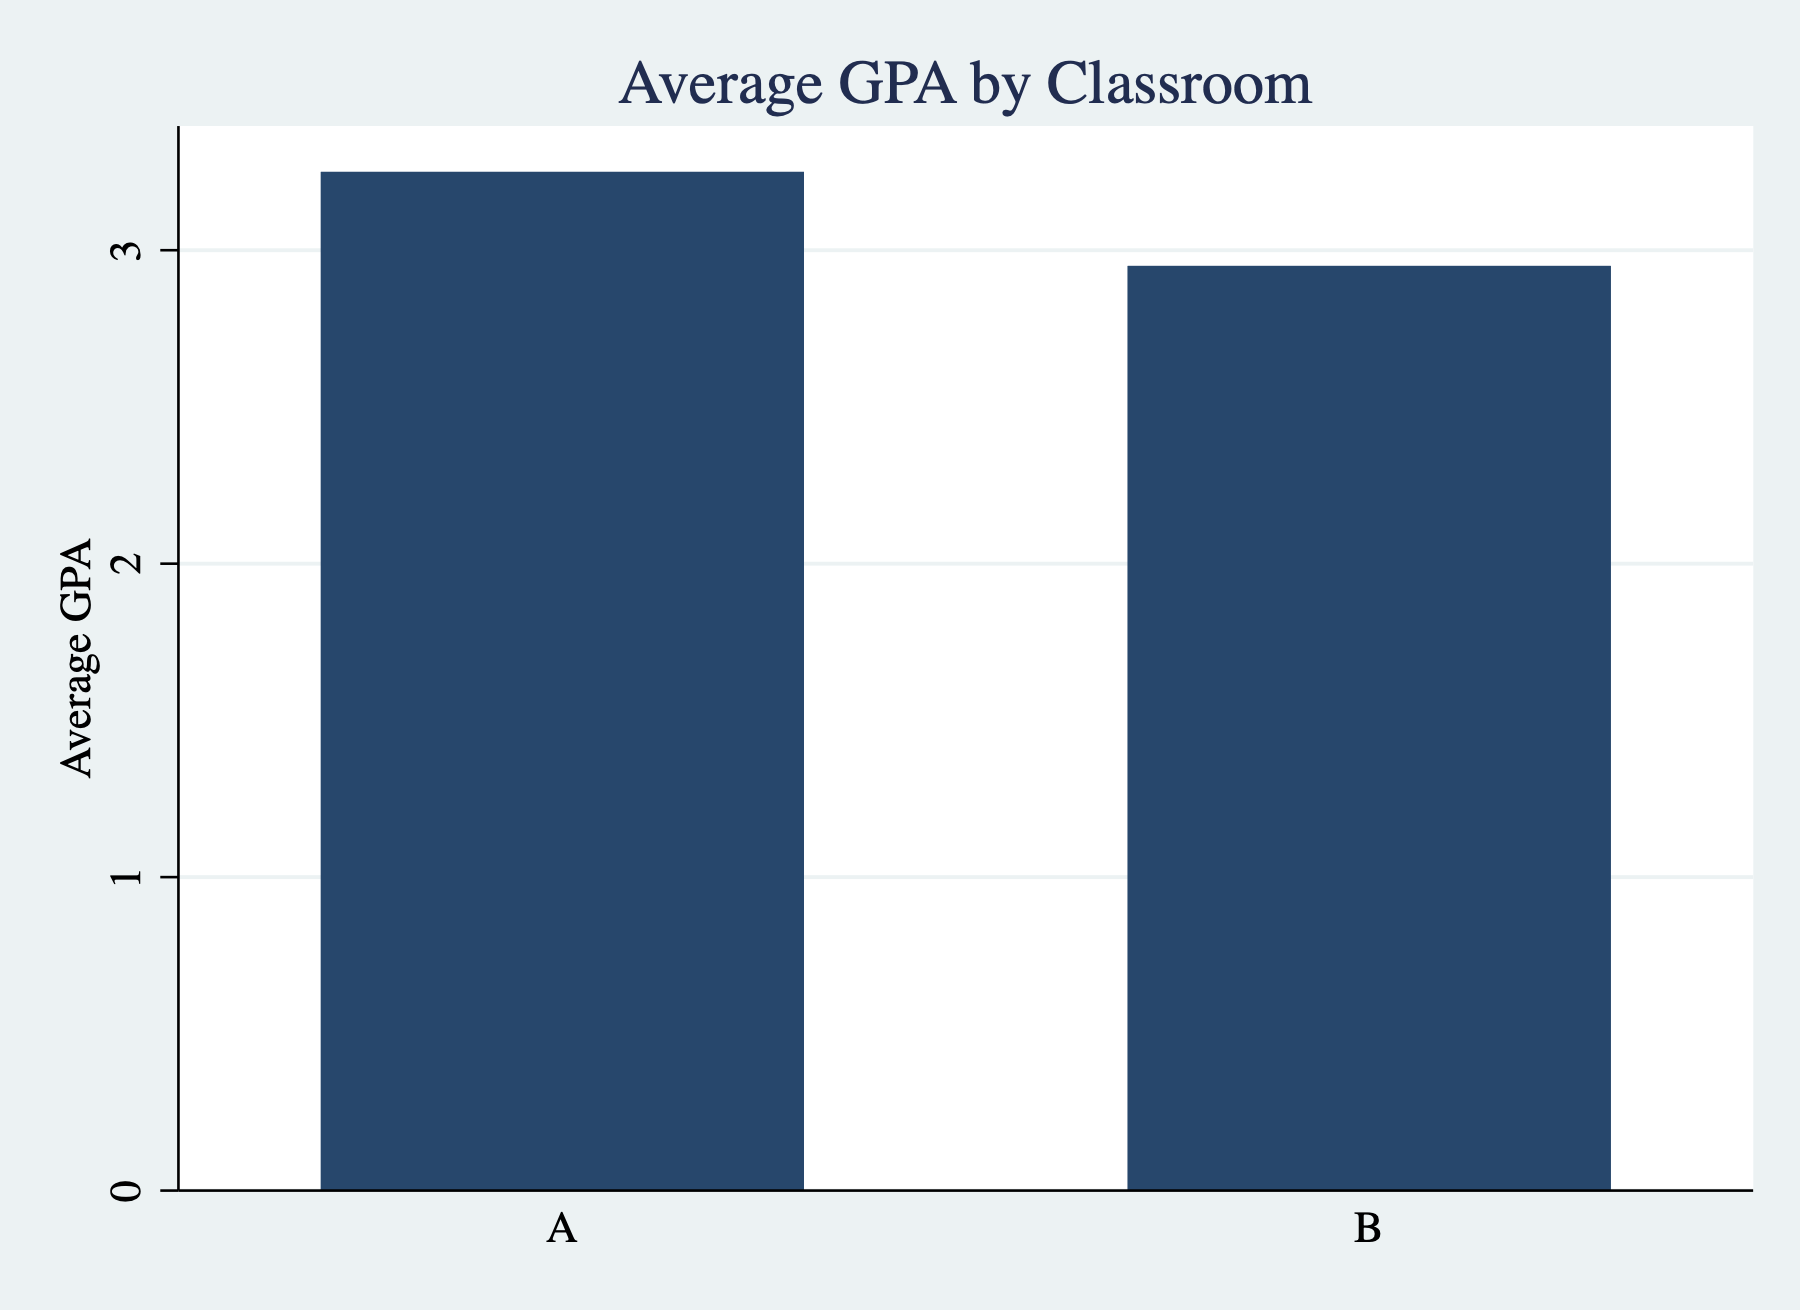
\includegraphics[width=0.65\linewidth]{images/03_bar_ex2} 

}

\caption{Simple Bar Graph with Titles/Labels}\label{fig:barex2}
\end{figure}

Sometimes we need to change the aesthetics of our figures to make them more easily readable. One external package I find useful to install is \texttt{blindschemes}, which provides color schemes for Stata graphs that are distinguishable for individuals that are color blind. To install blindschemes type:

\begin{Shaded}
\begin{Highlighting}[]
\KeywordTok{ssc}\NormalTok{ install blindschemes}
\end{Highlighting}
\end{Shaded}

\texttt{blindschemes} comes with a number of different \texttt{schemes}. You can think of graphics schemes as capturing the overall theme or aesthetic of your graph. Let's set the \texttt{scheme} to \texttt{plotplainblind}, which is one of the schemes that come from the \texttt{blindschemes} package.

\begin{Shaded}
\begin{Highlighting}[]
\KeywordTok{set} \DecValTok{scheme}\NormalTok{ plotplainblind}
\end{Highlighting}
\end{Shaded}

Now we can re-run the exact same code as before, but the overall aesthetic will be different. This is because we have changed the scheme of the graph.

\begin{Shaded}
\begin{Highlighting}[]
\KeywordTok{graph} \BaseNTok{bar}\NormalTok{ (}\KeywordTok{mean}\NormalTok{) gpa, }\BaseNTok{over}\NormalTok{(school) }\CommentTok{///}
    \BaseNTok{title}\NormalTok{(}\StringTok{"Average GPA by Classroom"}\NormalTok{) }\CommentTok{///}
    \BaseNTok{ytitle}\NormalTok{(}\StringTok{"Average GPA"}\NormalTok{) }
\end{Highlighting}
\end{Shaded}

\begin{figure}

{\centering 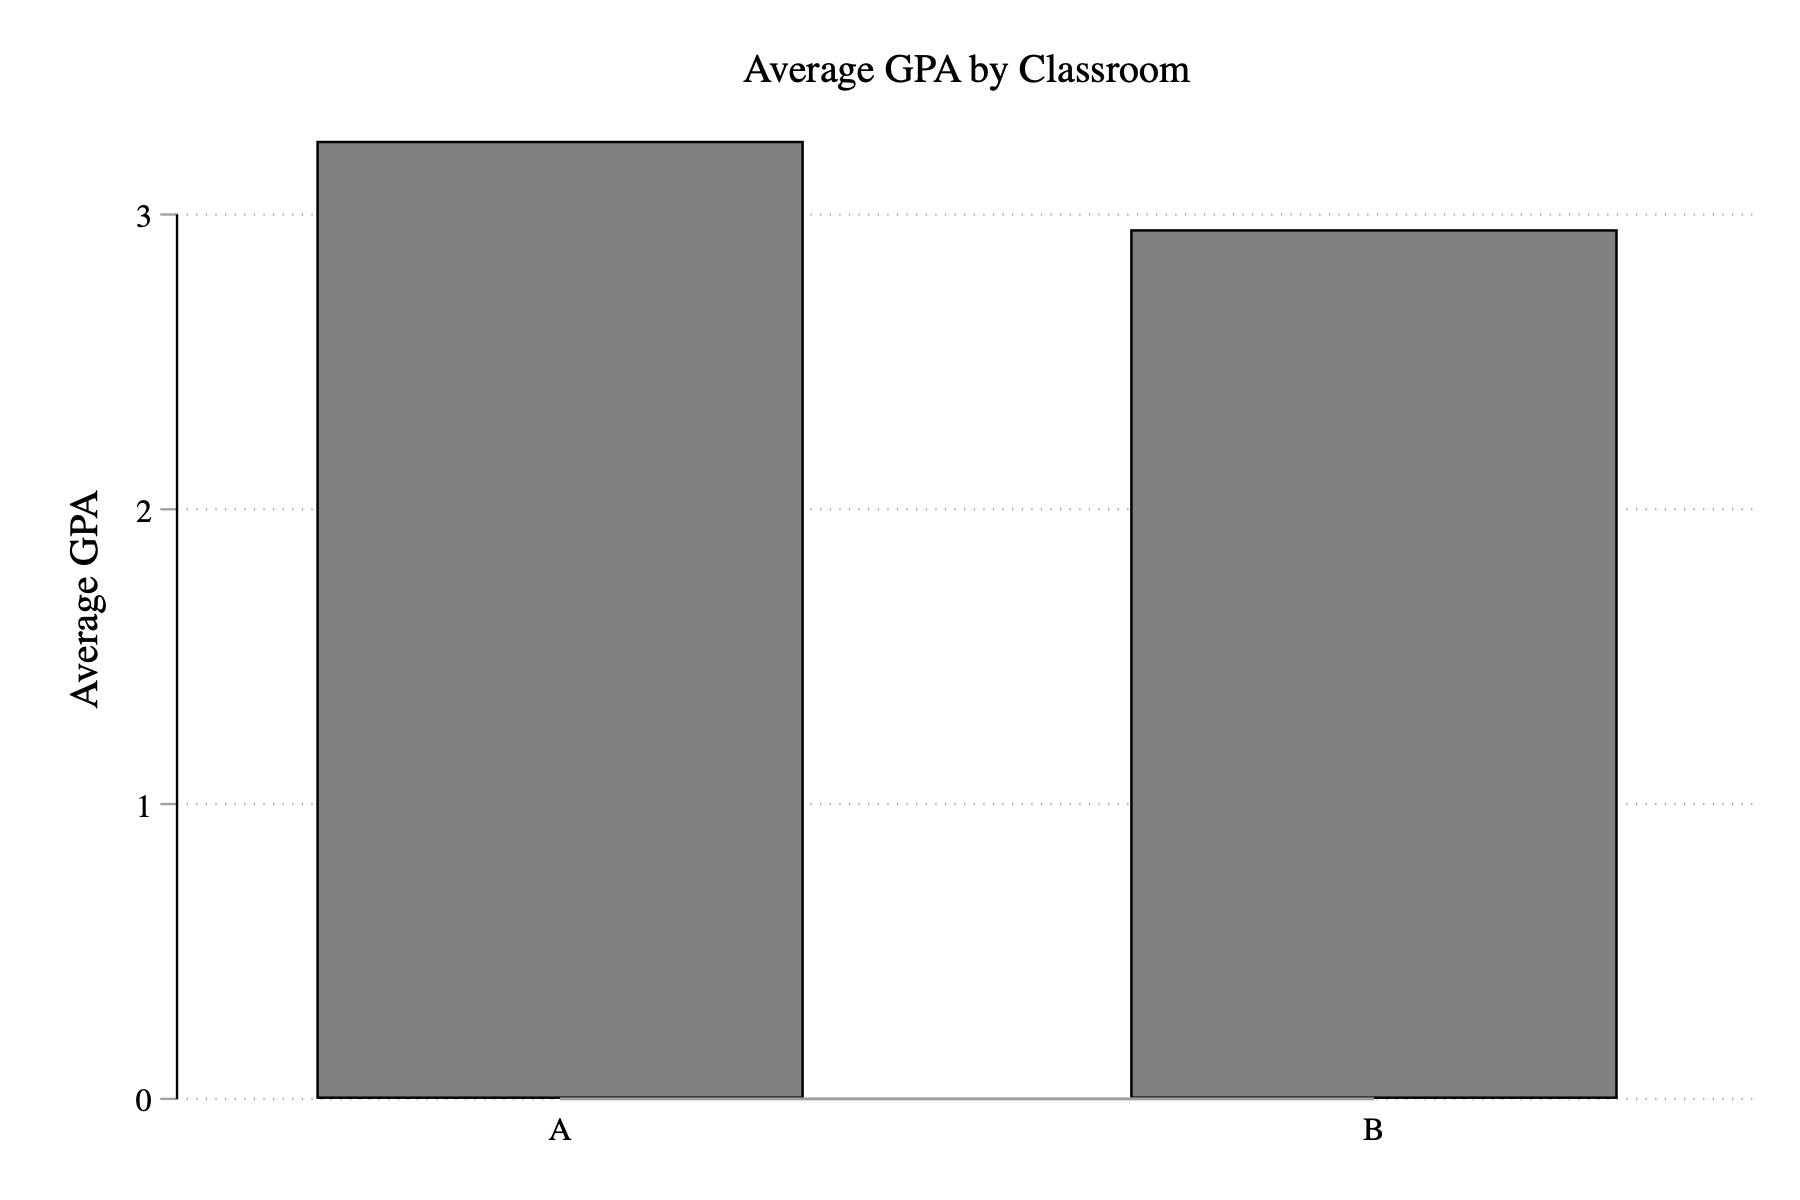
\includegraphics[width=0.65\linewidth]{images/03_bar_ex3} 

}

\caption{Simple Bar Graph with Titles/Labels}\label{fig:barex3}
\end{figure}

There are many further options when constructing bar graphs. Sometimes, the option you are looking for isn't available, but there are still ways to construct the required bar graph. In other words, you may need to use some \textbf{data wrangling} to get your data in the right format to construct a bar graph. In the next section, we will learn another data-wrangling technique that is generally useful, but will be particularly useful for generating the bar graph we need in order to visualize the veil of darkness test.

\section{Collapse}\label{collapse}

The \texttt{collapse} command transforms your data to a different unit of analysis. Why is this useful? Imagine you have individual-level data on income, but you only care about average income by state for your analysis. The \texttt{collapse} command will allow you to quickly transform your data to the state level. Imagine you want to understand averages of a variable over the years. Collapsing the data to the year level can be a quick way to understand how the variable is changing over time. When you have a lot of data, collapsing the data first may make your code much more efficient.

The basic syntax of the \texttt{collapse} command is

\begin{Shaded}
\begin{Highlighting}[]
\KeywordTok{collapse}\NormalTok{ (stat) varlist1, }\KeywordTok{by}\NormalTok{(varlist2)}
\end{Highlighting}
\end{Shaded}

\texttt{(stat)} will be some statistic. The default is the mean. We will also use \texttt{count} later in this chapter. \texttt{varlist1} is a variable (or list of variables) that you would like to retrieve the mean for. \texttt{varlist2} is a variable (or list of variables) will define the groups over which the statistic is calculated.

To practice with this command, consider the (fake) dataset below:

\begin{figure}

{\centering 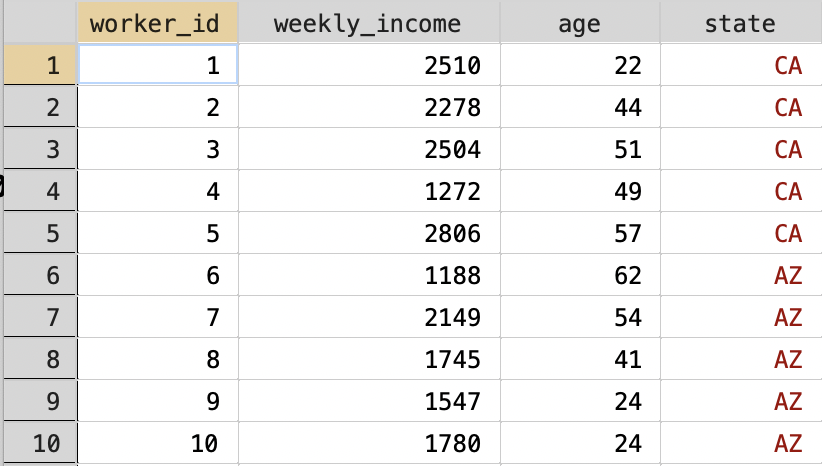
\includegraphics[width=0.65\linewidth]{images/03_wages} 

}

\caption{Wages for Workers in Different States}\label{fig:wages}
\end{figure}

Our goal now is to transform this dataset into a dataset with just two observations: one for ``CA'' and one for ``AZ''. In terms of variables, we want two variables, one that contains the average weekly income and one that contains the average age. In other words, we are taking a dataset that is currently at the worker level and collapsing it to a dataset that is at the state level. To do this in Stata we type:

\begin{Shaded}
\begin{Highlighting}[]
\KeywordTok{collapse}\NormalTok{ (}\KeywordTok{mean}\NormalTok{) weekly\_income age, }\KeywordTok{by}\NormalTok{(state)}
\end{Highlighting}
\end{Shaded}

The collapsed dataset is depicted in Figure \ref{fig:collapsed}

\begin{figure}

{\centering 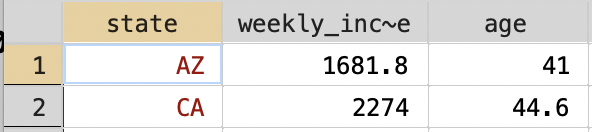
\includegraphics[width=0.65\linewidth]{images/03_wages2} 

}

\caption{Collapsed State-level Dataset}\label{fig:collapsed}
\end{figure}

One important note is that in order to retrieve the original dataset, you would need to re-load it into Stata. There is no simple ``undo'' button that gets you back to the original worker-level dataset.

\section{Visualizing Veil of Darkness}\label{visualizing-veil-of-darkness}

In this section, we want to construct a data visualization that will allow us clearly see the results of the veil of darkness test. Let's look at some hypothetical examples before we begin so that we know what our end goal should look like. Figure \ref{fig:veilhyp1} presents a hypothetical example of what our results could look like.

\begin{figure}

{\centering 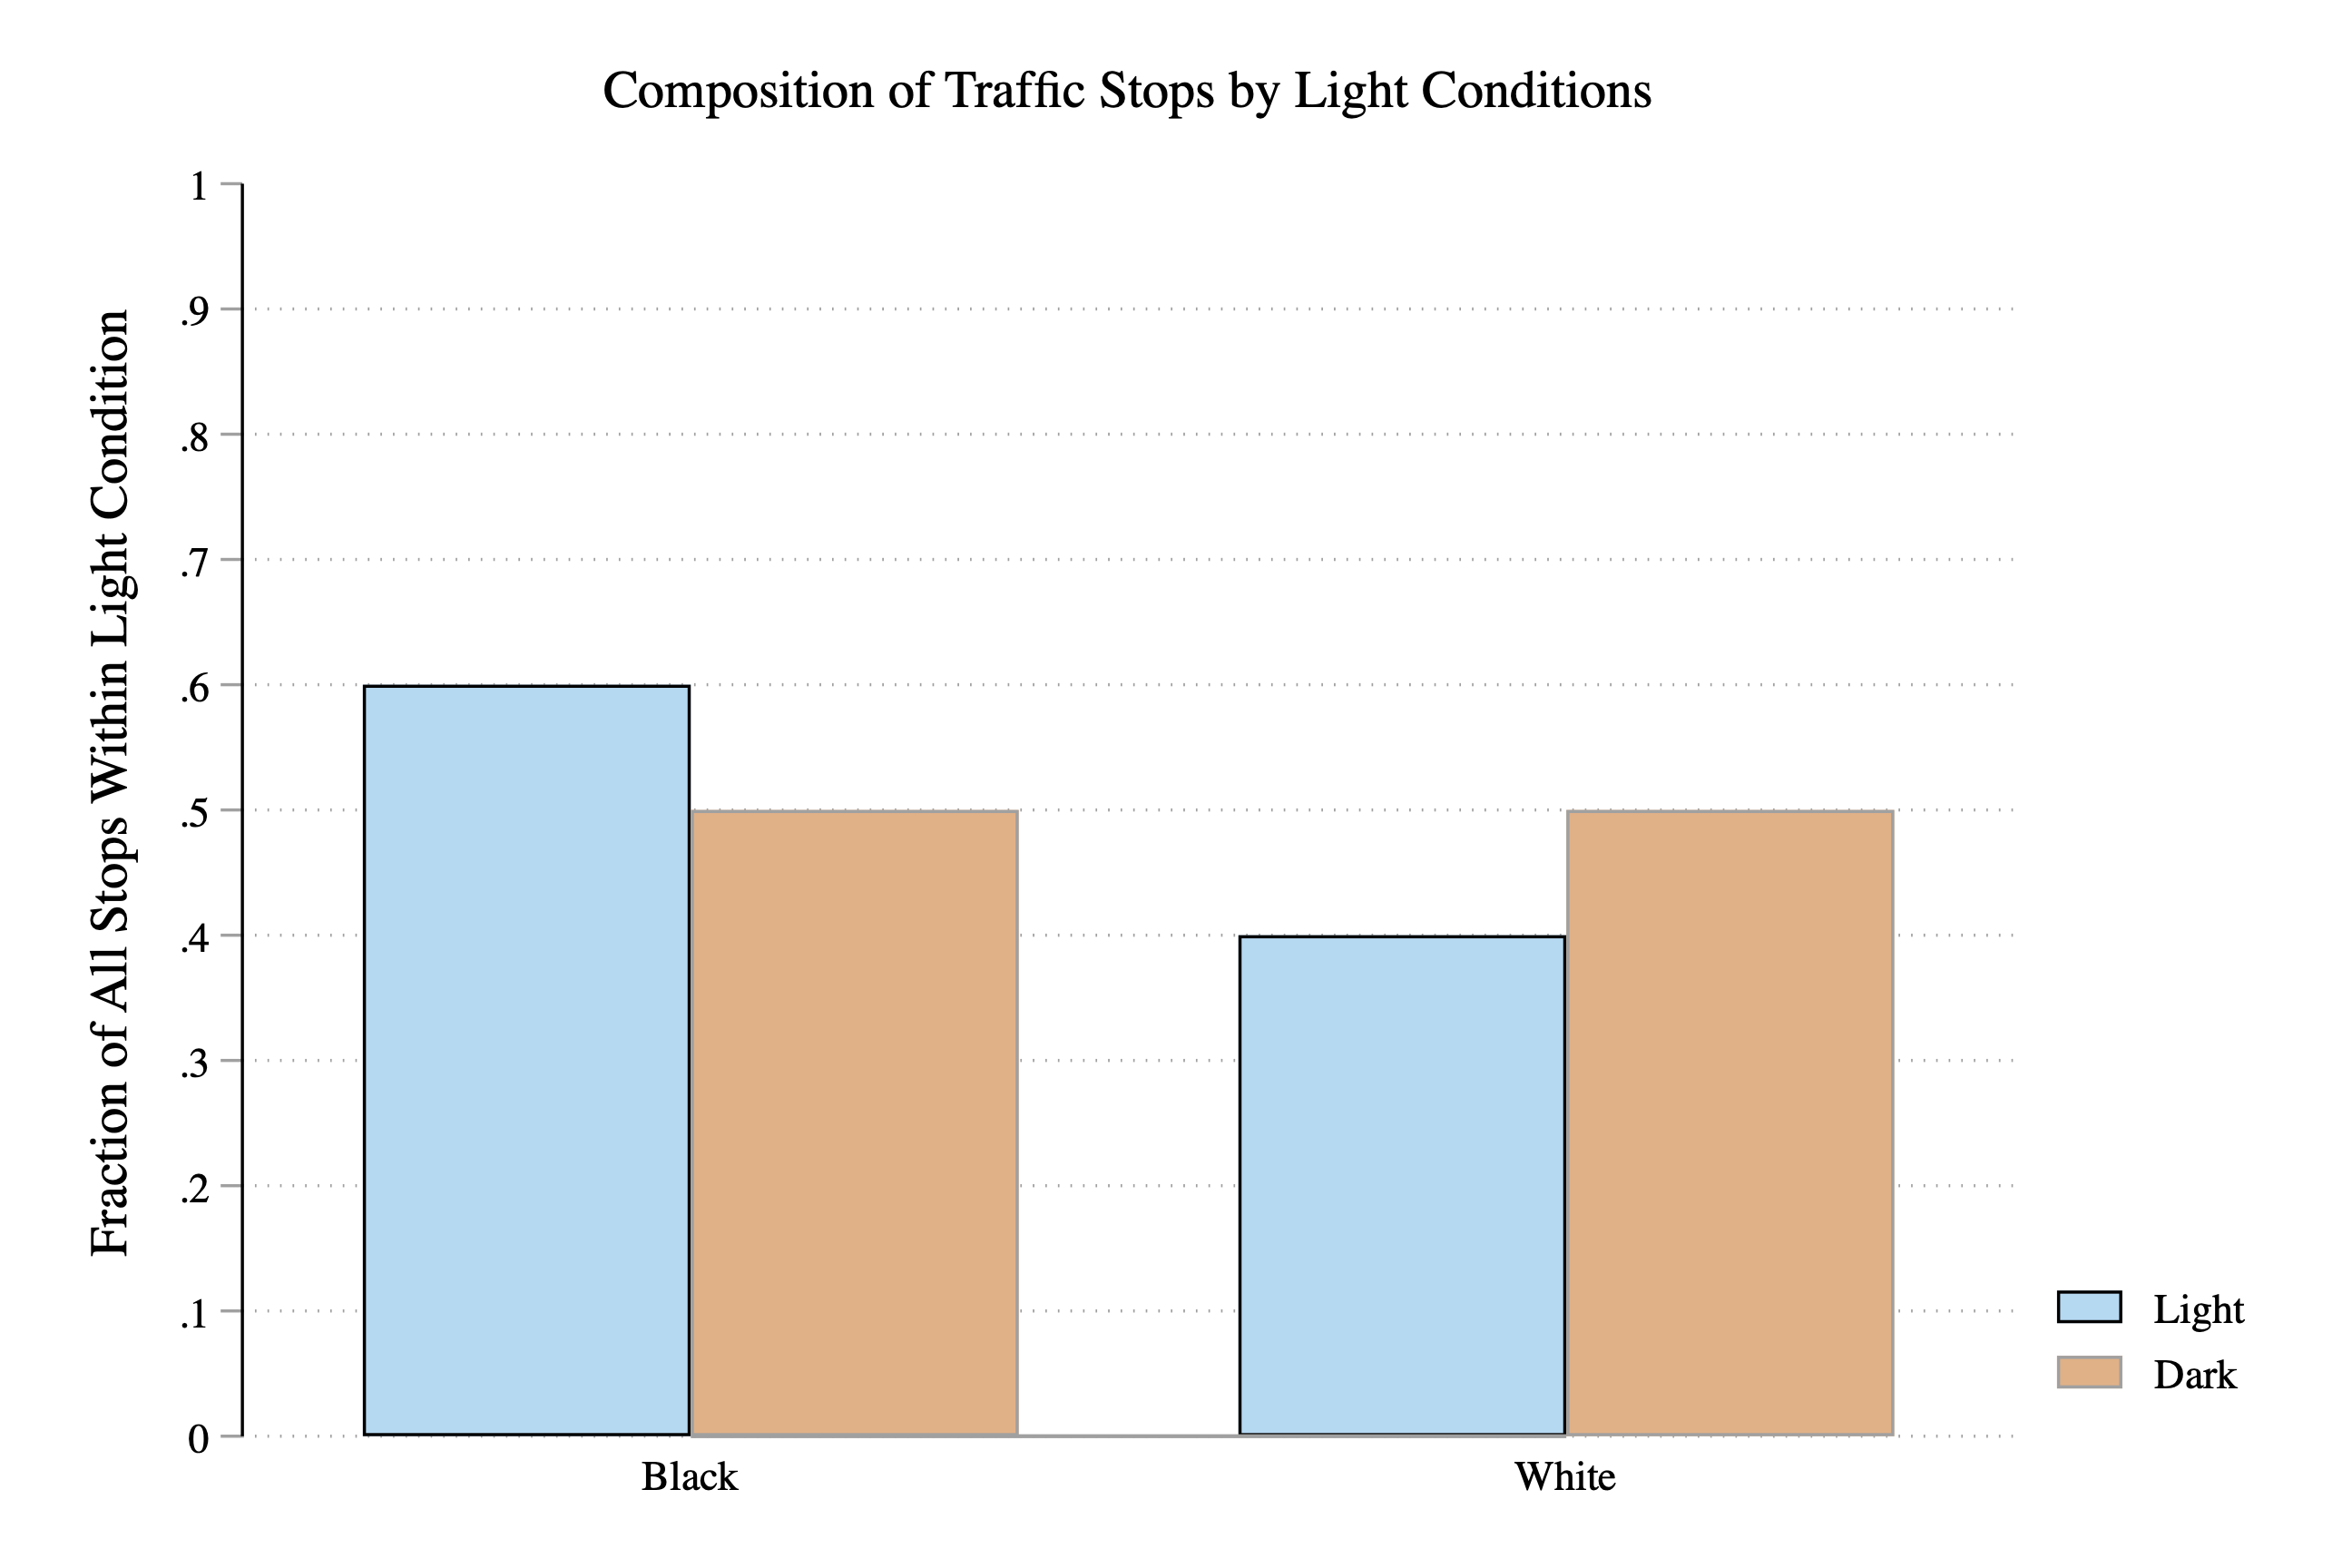
\includegraphics[width=0.65\linewidth]{images/03_ill_ex1} 

}

\caption{Veil of Darkness Test Finds Discriminatory Policy Behavior}\label{fig:veilhyp1}
\end{figure}

Is this evidence of discriminatory behavior or not? In this case, the answer is yes. When it is light out, 60 percent of stopped drivers are Black. When it is dark out, this falls to 50 percent. The fall in the fraction of stops for Black drivers in the darkness could be explained by discriminatory officers being unable to observe race in the dark, and thus, unable to target minority drivers for stops. Before continuing, make sure you understand what data is being presented in Figure \ref{fig:veilhyp1} above.

Figure \ref{fig:veilhyp2} presents a different hypothetical example of what the bar graph might look like.

\begin{figure}

{\centering 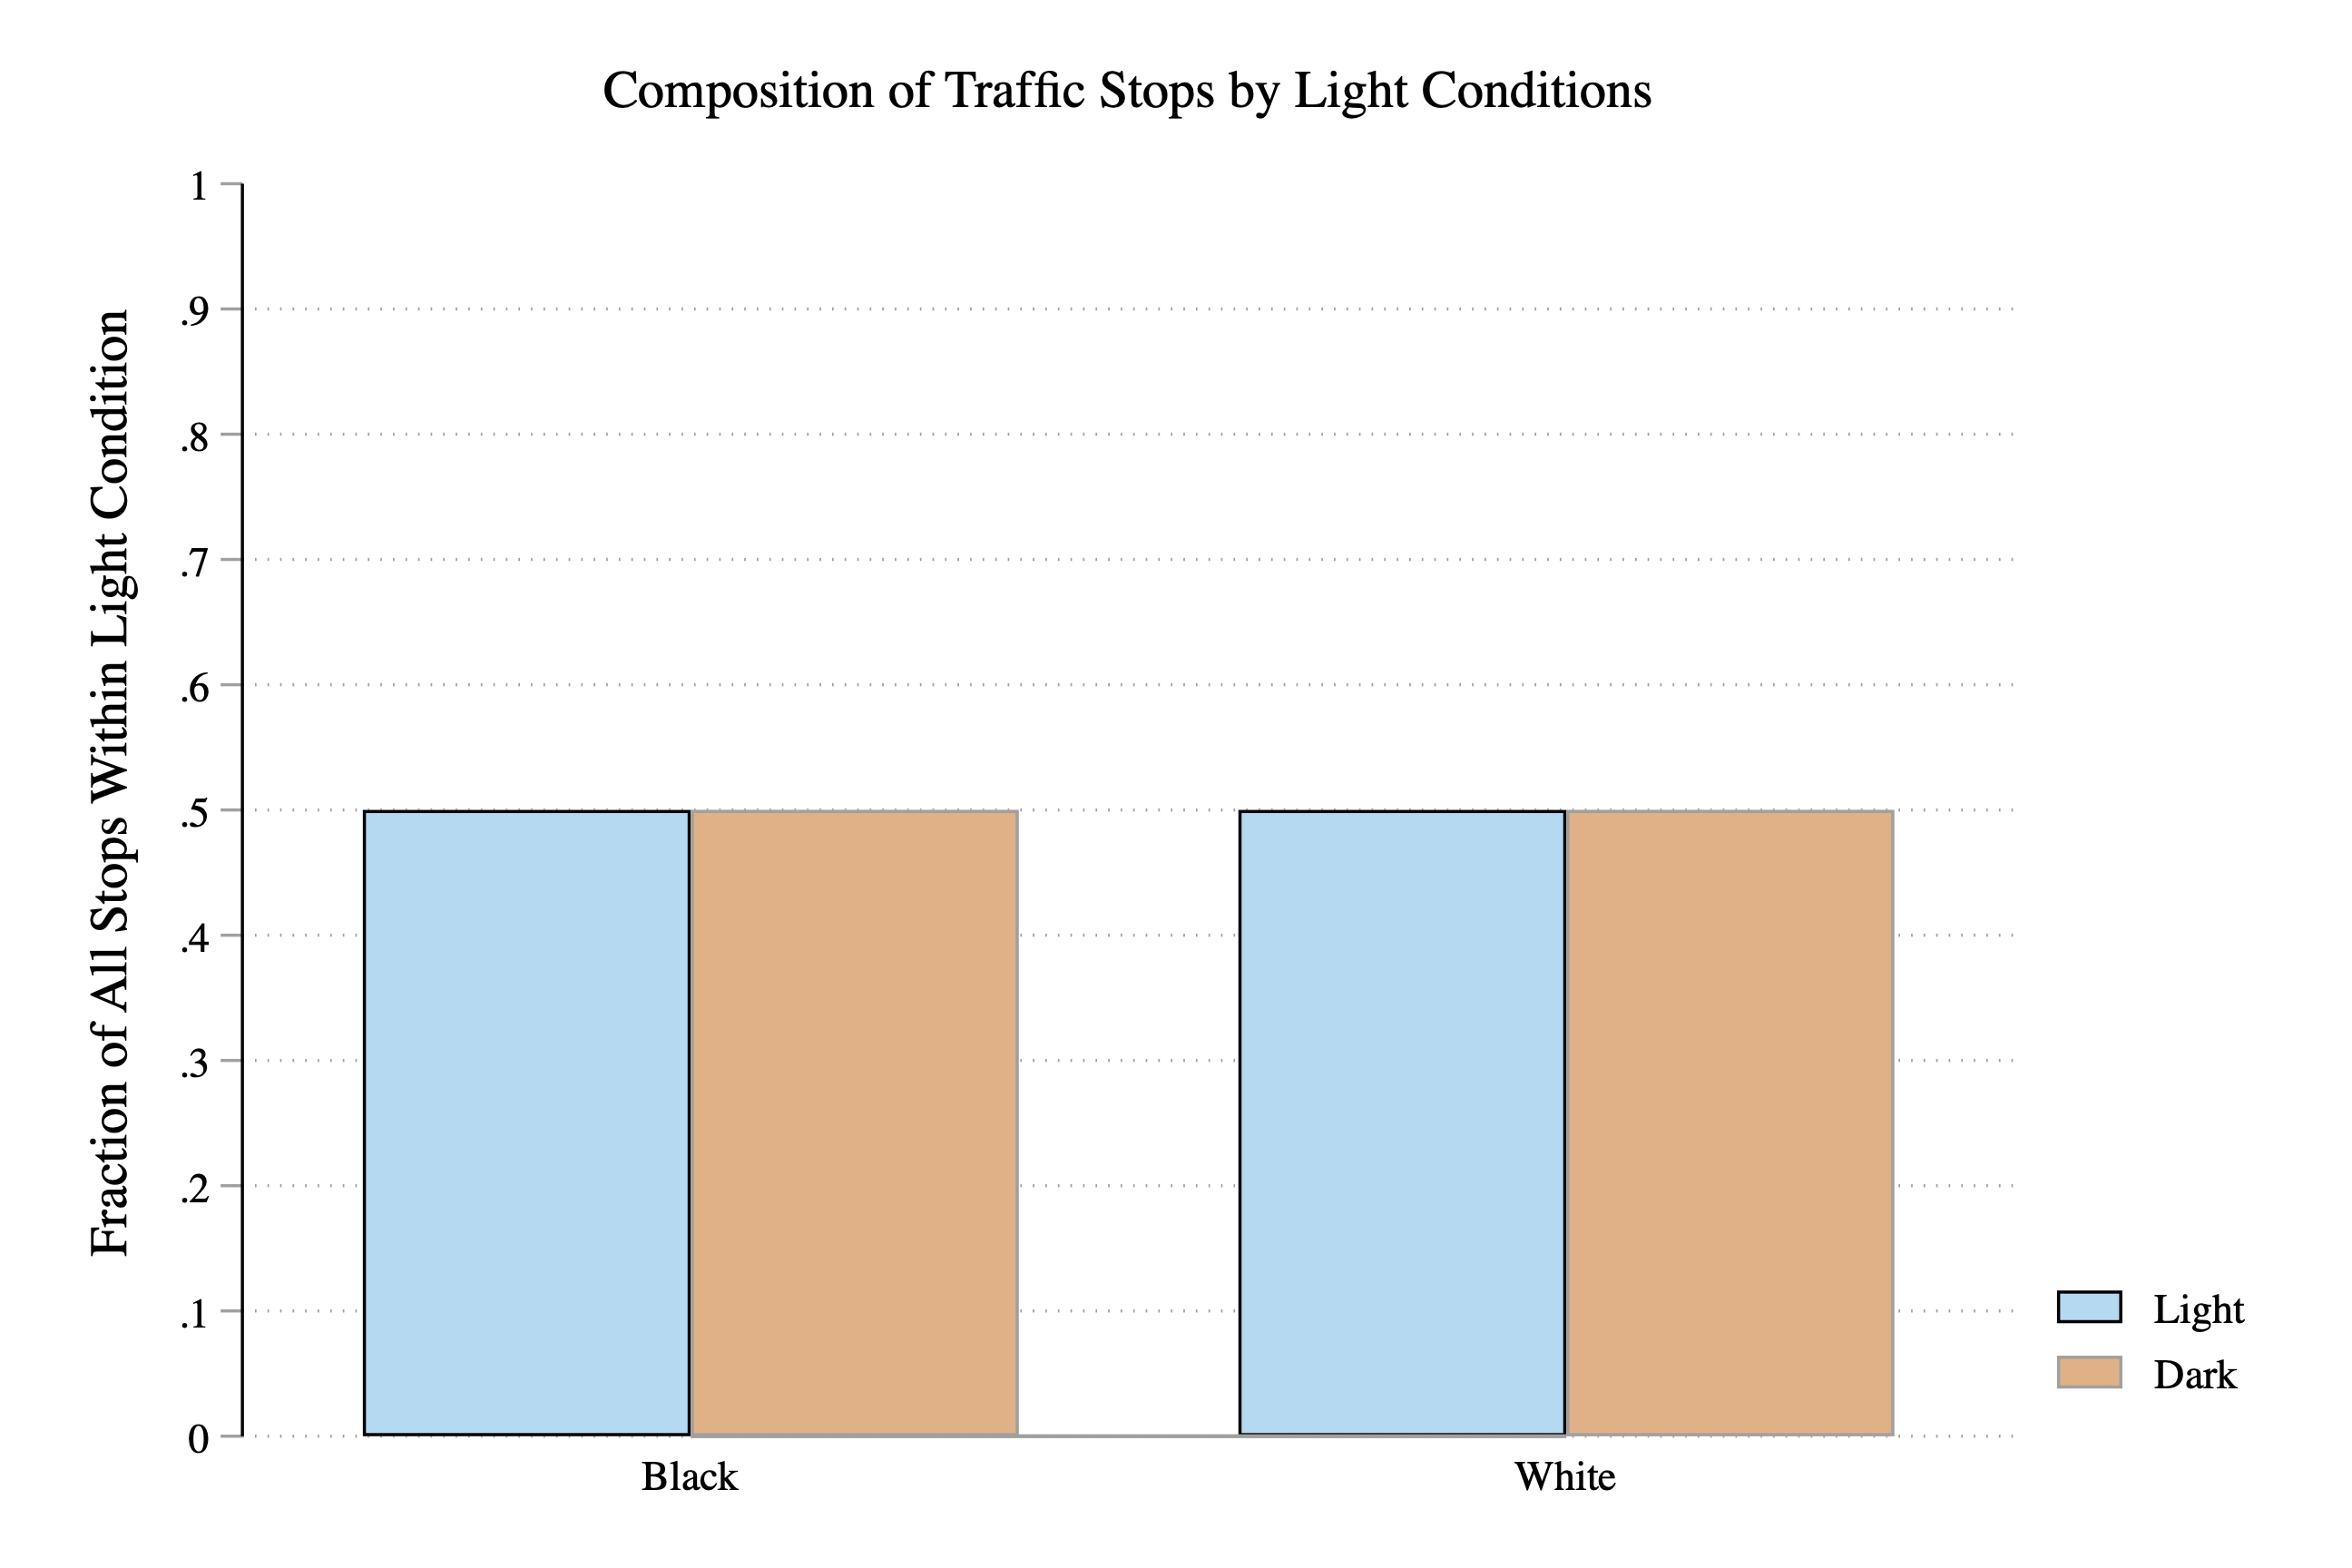
\includegraphics[width=0.65\linewidth]{images/03_ill_ex2} 

}

\caption{Veil of Darkness Test Finds No Evidence of Discriminatory Policy Behavior}\label{fig:veilhyp2}
\end{figure}

Is this evidence of discriminatory behavior or not? In this case, the answer is no. When it is light out, 50 percent of stopped drivers are Black. When it is dark out, this remains steady at 50 percent. It does not appear in this data that officers are targeting minority drivers during the day.

Starting where we left off, we have now constructed a dataset with (1) traffic stops that occur between 6:30-7:00 PM, and (2) indicators for whether there was sunlight (\texttt{dark==0}) or darkness (\texttt{dark==1}). We can use this data to generate a similar visualization as the graphs above.

We need to compare the composition of traffic stops in times of sunlight vs.~darkness. We can use the \texttt{collapse} command to create a dataset of these statistics. To start, let's create a dataset that has the number of stops by race, in both daylight and darkness.

To count the number of observations per race for both daylight and darkness, we can use the \texttt{count} option of the collapse command. This option will count the number of observations with non-missing values of a variable. To begin, let's create a variable (that will eventually store our counts) that is non-missing for all observations.

\begin{Shaded}
\begin{Highlighting}[]
\KeywordTok{gen}\NormalTok{ obs\_count = 1}
\end{Highlighting}
\end{Shaded}

Now it might not be immediately clear why we have created this variable. Right now it is just a variable that is equal to 1 for every observation. However, once we collapse the data, this variable will hold the information we need to construct our bar graph. To collapse the data to the subject-race-by-dark condition level:

\begin{Shaded}
\begin{Highlighting}[]
\KeywordTok{collapse}\NormalTok{ (}\FunctionTok{count}\NormalTok{) obs\_count, }\KeywordTok{by}\NormalTok{(subject\_race dark) }
\end{Highlighting}
\end{Shaded}

When we specify two variables in \texttt{by}, the resulting dataset includes an observation for every unique combination of the two variables. In our dataset, there are 5 different values of the \texttt{race} variable, while there are 2 different values of our \texttt{dark} variable. The resulting dataset in this case will have 10 observations. Each row will correspond to a given race in a given light condition.

Figure \ref{fig:br1} displays the resulting collapsed dataset. As you can see, for each race and light condition, we now have the total number of stops that occurred for that race, within the given light condition. For example, the first row here indicates that in our dataset, there are 375 stops for Asian/Pacific Islanders when it is between 6:30-7:00 PM and light out (i.e.~\texttt{dark==0}).

\begin{figure}

{\centering 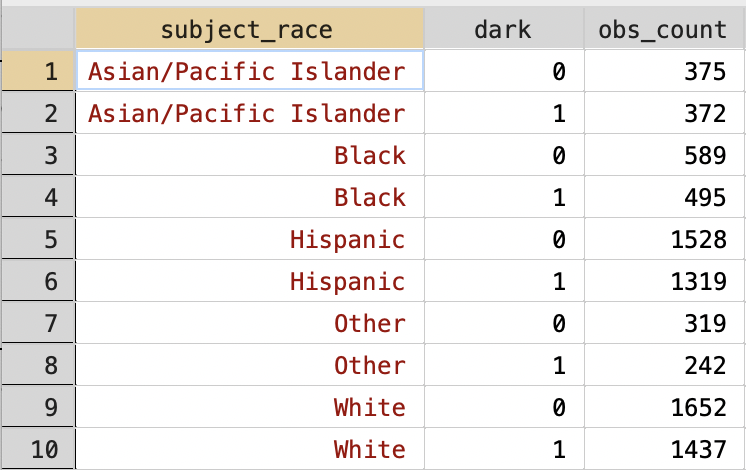
\includegraphics[width=0.65\linewidth]{images/03_br1} 

}

\caption{Collapsed Dataset}\label{fig:br1}
\end{figure}

In our plot, however, we want to plot the fraction of stops for each race by light condition. This is a pretty small dataset, so we could do this manually. For example, what fraction of stops when it is light out are for Asian/Pacific Islanders. Based on \ref{fig:br1}, we know that this equal to:

\[ 
\frac{\text{Stops for Asian/Pacific Islander When Light}}{\text{Stops When Light}} = \\ \frac{375}{375+589+1528+319+1652} =  0.084
\]
But what if we had more observations. Also, we need these values in our dataset. It will be easier if we can add a variable to the dataset that contains this information. We are going to do this in two steps. First, we are going to create a variable that contains the total stops within a given light condition. Then, we are going to generate the variable we want by dividing \texttt{obs\_count} by this new variable.

To create this new variable we are going to use the \texttt{egen} command. \texttt{egen} stands for extensions to generate, and is very useful when trying to create new variables. If you ever want to create a variable, but can't figure out exactly how, type \texttt{help\ egen} to see if it is possible with the egen command.

First, let's present the code for calculating total stops by light condition, before explaining how it works:

\begin{Shaded}
\begin{Highlighting}[]
\KeywordTok{bysort}\NormalTok{ dark: }\KeywordTok{egen}\NormalTok{ total\_obs = }\KeywordTok{total}\NormalTok{(obs\_count)}
\end{Highlighting}
\end{Shaded}

\texttt{bysort\ dark:} tells Stata that any code that comes after the \texttt{:} should be done separately for values of the \texttt{dark} variable. \texttt{egen\ total\_obs\ =\ total(obs\_count)} will create a new variable that is equal to the sum total of the variable \texttt{obs\_count}. In simple terms, the total number of stops in daylight and darkness. Let's look at the resulting dataset. Make sure you understand what \texttt{total\_obs} represents before moving on to the next section.

\begin{figure}

{\centering 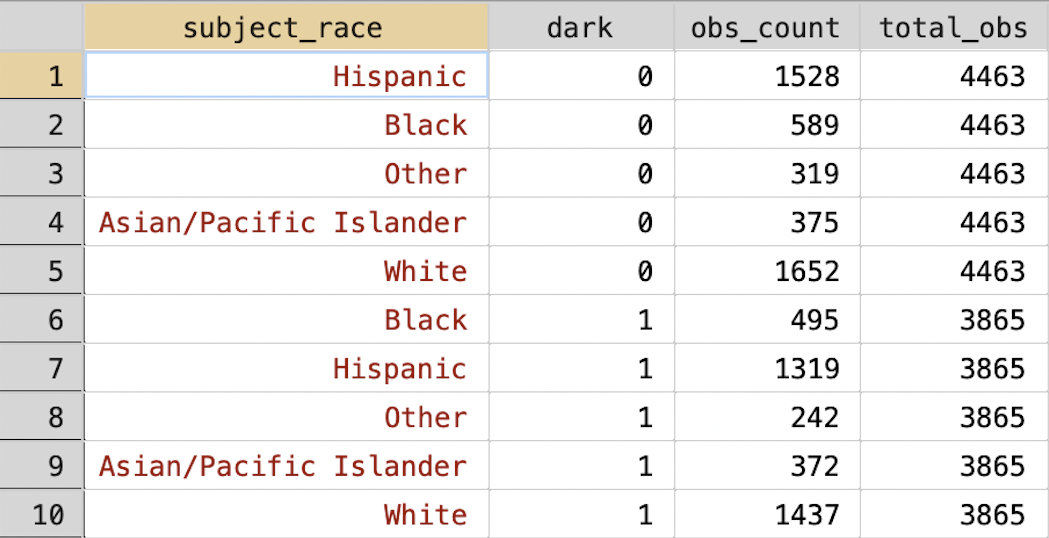
\includegraphics[width=0.65\linewidth]{images/03_br1p5} 

}

\caption{Collapsed Dataset with Total Stops by Light Condition}\label{fig:br1p5}
\end{figure}

Now that we have (1) total stops by race in daylight vs.~darkness and (2) total stops overall in daylight vs.~darkness we can create our required variables:

\begin{Shaded}
\begin{Highlighting}[]
  \KeywordTok{gen}\NormalTok{ fraction\_stops = obs\_count/total\_obs}
\end{Highlighting}
\end{Shaded}

Now we can use this variable to show the composition of traffic stops (by race) both in the daylight and in the darkness:

\begin{Shaded}
\begin{Highlighting}[]
\KeywordTok{graph} \BaseNTok{bar}\NormalTok{ fraction\_stops, }\BaseNTok{over}\NormalTok{(dark) }\BaseNTok{over}\NormalTok{(subject\_race)}
\end{Highlighting}
\end{Shaded}

\begin{figure}

{\centering 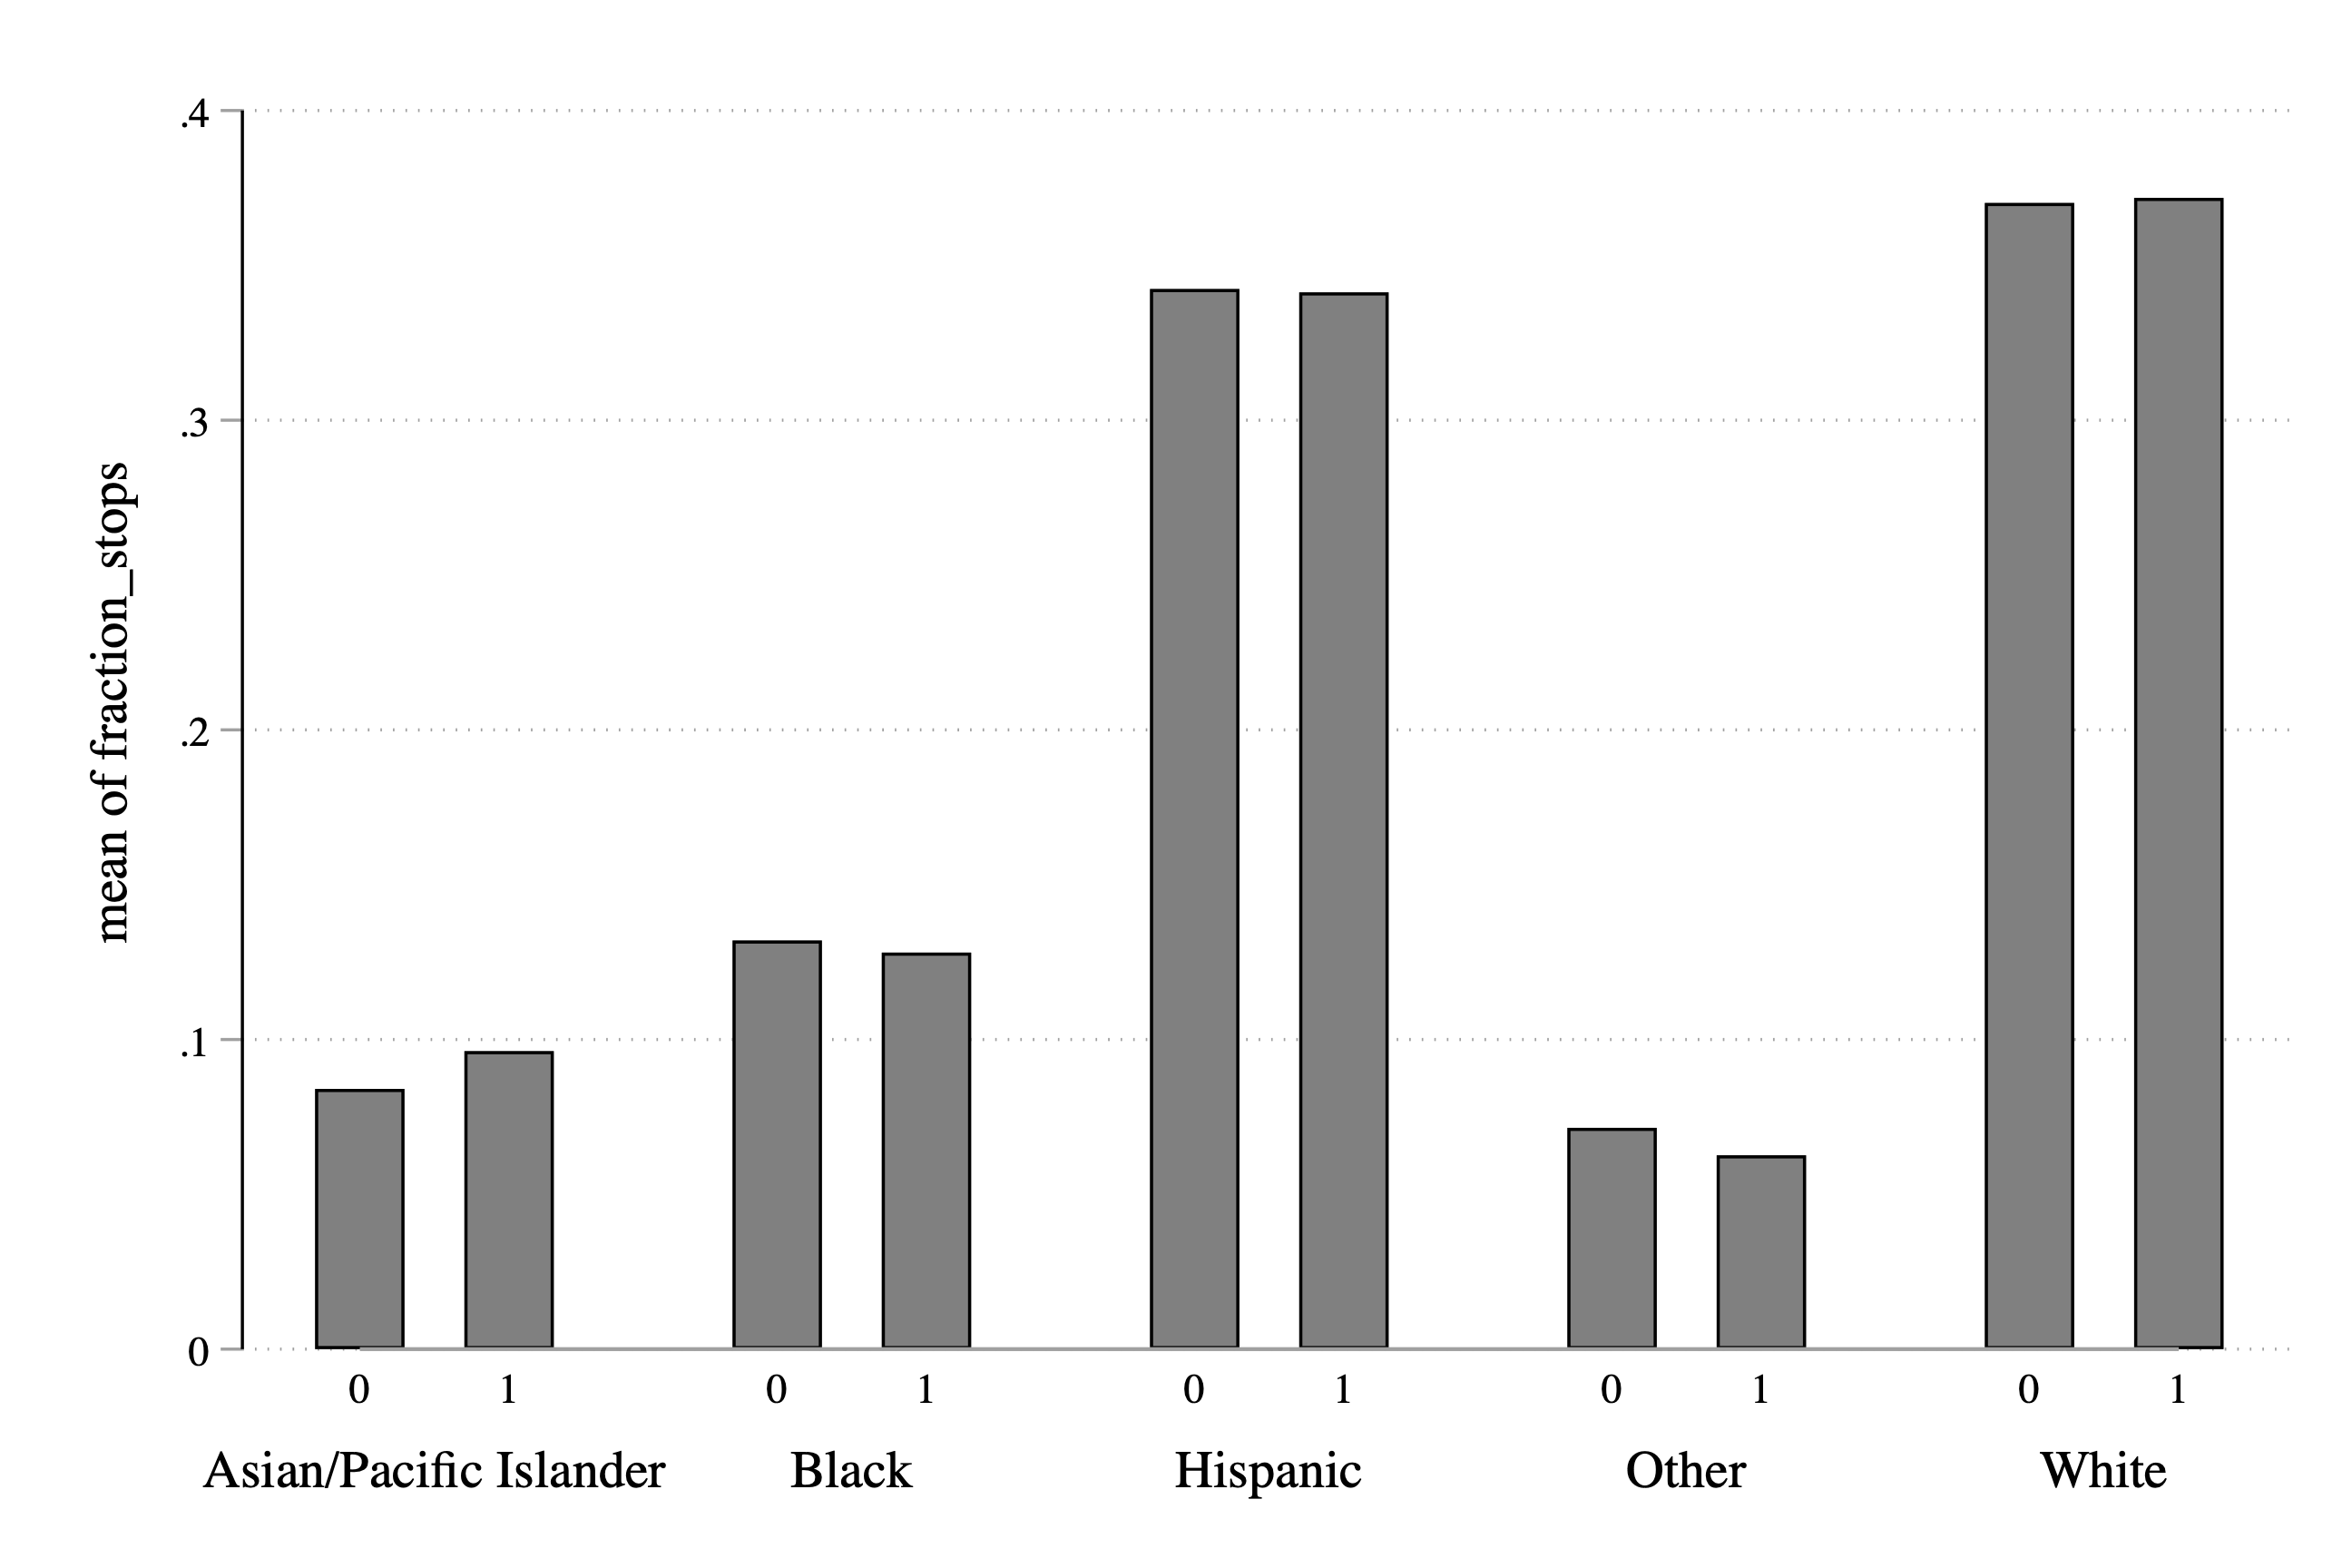
\includegraphics[width=0.65\linewidth]{images/03_bar1} 

}

\caption{Fraction of Stops by Race and Light Condition}\label{fig:bar1}
\end{figure}

This is a good start. It has all the information we need. However, it would be next to impossible for an external reader to understand what the information presented means. What is a 0 and a 1? What is the bar graph actually showing? The next section will introduce a few things to improve our data visualization so that it is interpretable to a reader.

\section{Improving Aesthetics}\label{improving-aesthetics}

As always, the first task is to add some descriptive titles and labels:

\begin{Shaded}
\begin{Highlighting}[]
\KeywordTok{graph} \BaseNTok{bar}\NormalTok{ fraction, }\BaseNTok{over}\NormalTok{(dark) }\BaseNTok{over}\NormalTok{(subject\_race) }\CommentTok{///}
    \BaseNTok{title}\NormalTok{(}\StringTok{"Composition of Traffic Stops by Light Conditions"}\NormalTok{) }\CommentTok{///}
    \BaseNTok{ytitle}\NormalTok{(}\StringTok{"Fraction of All Stops"}\NormalTok{) }
\end{Highlighting}
\end{Shaded}

\begin{figure}

{\centering 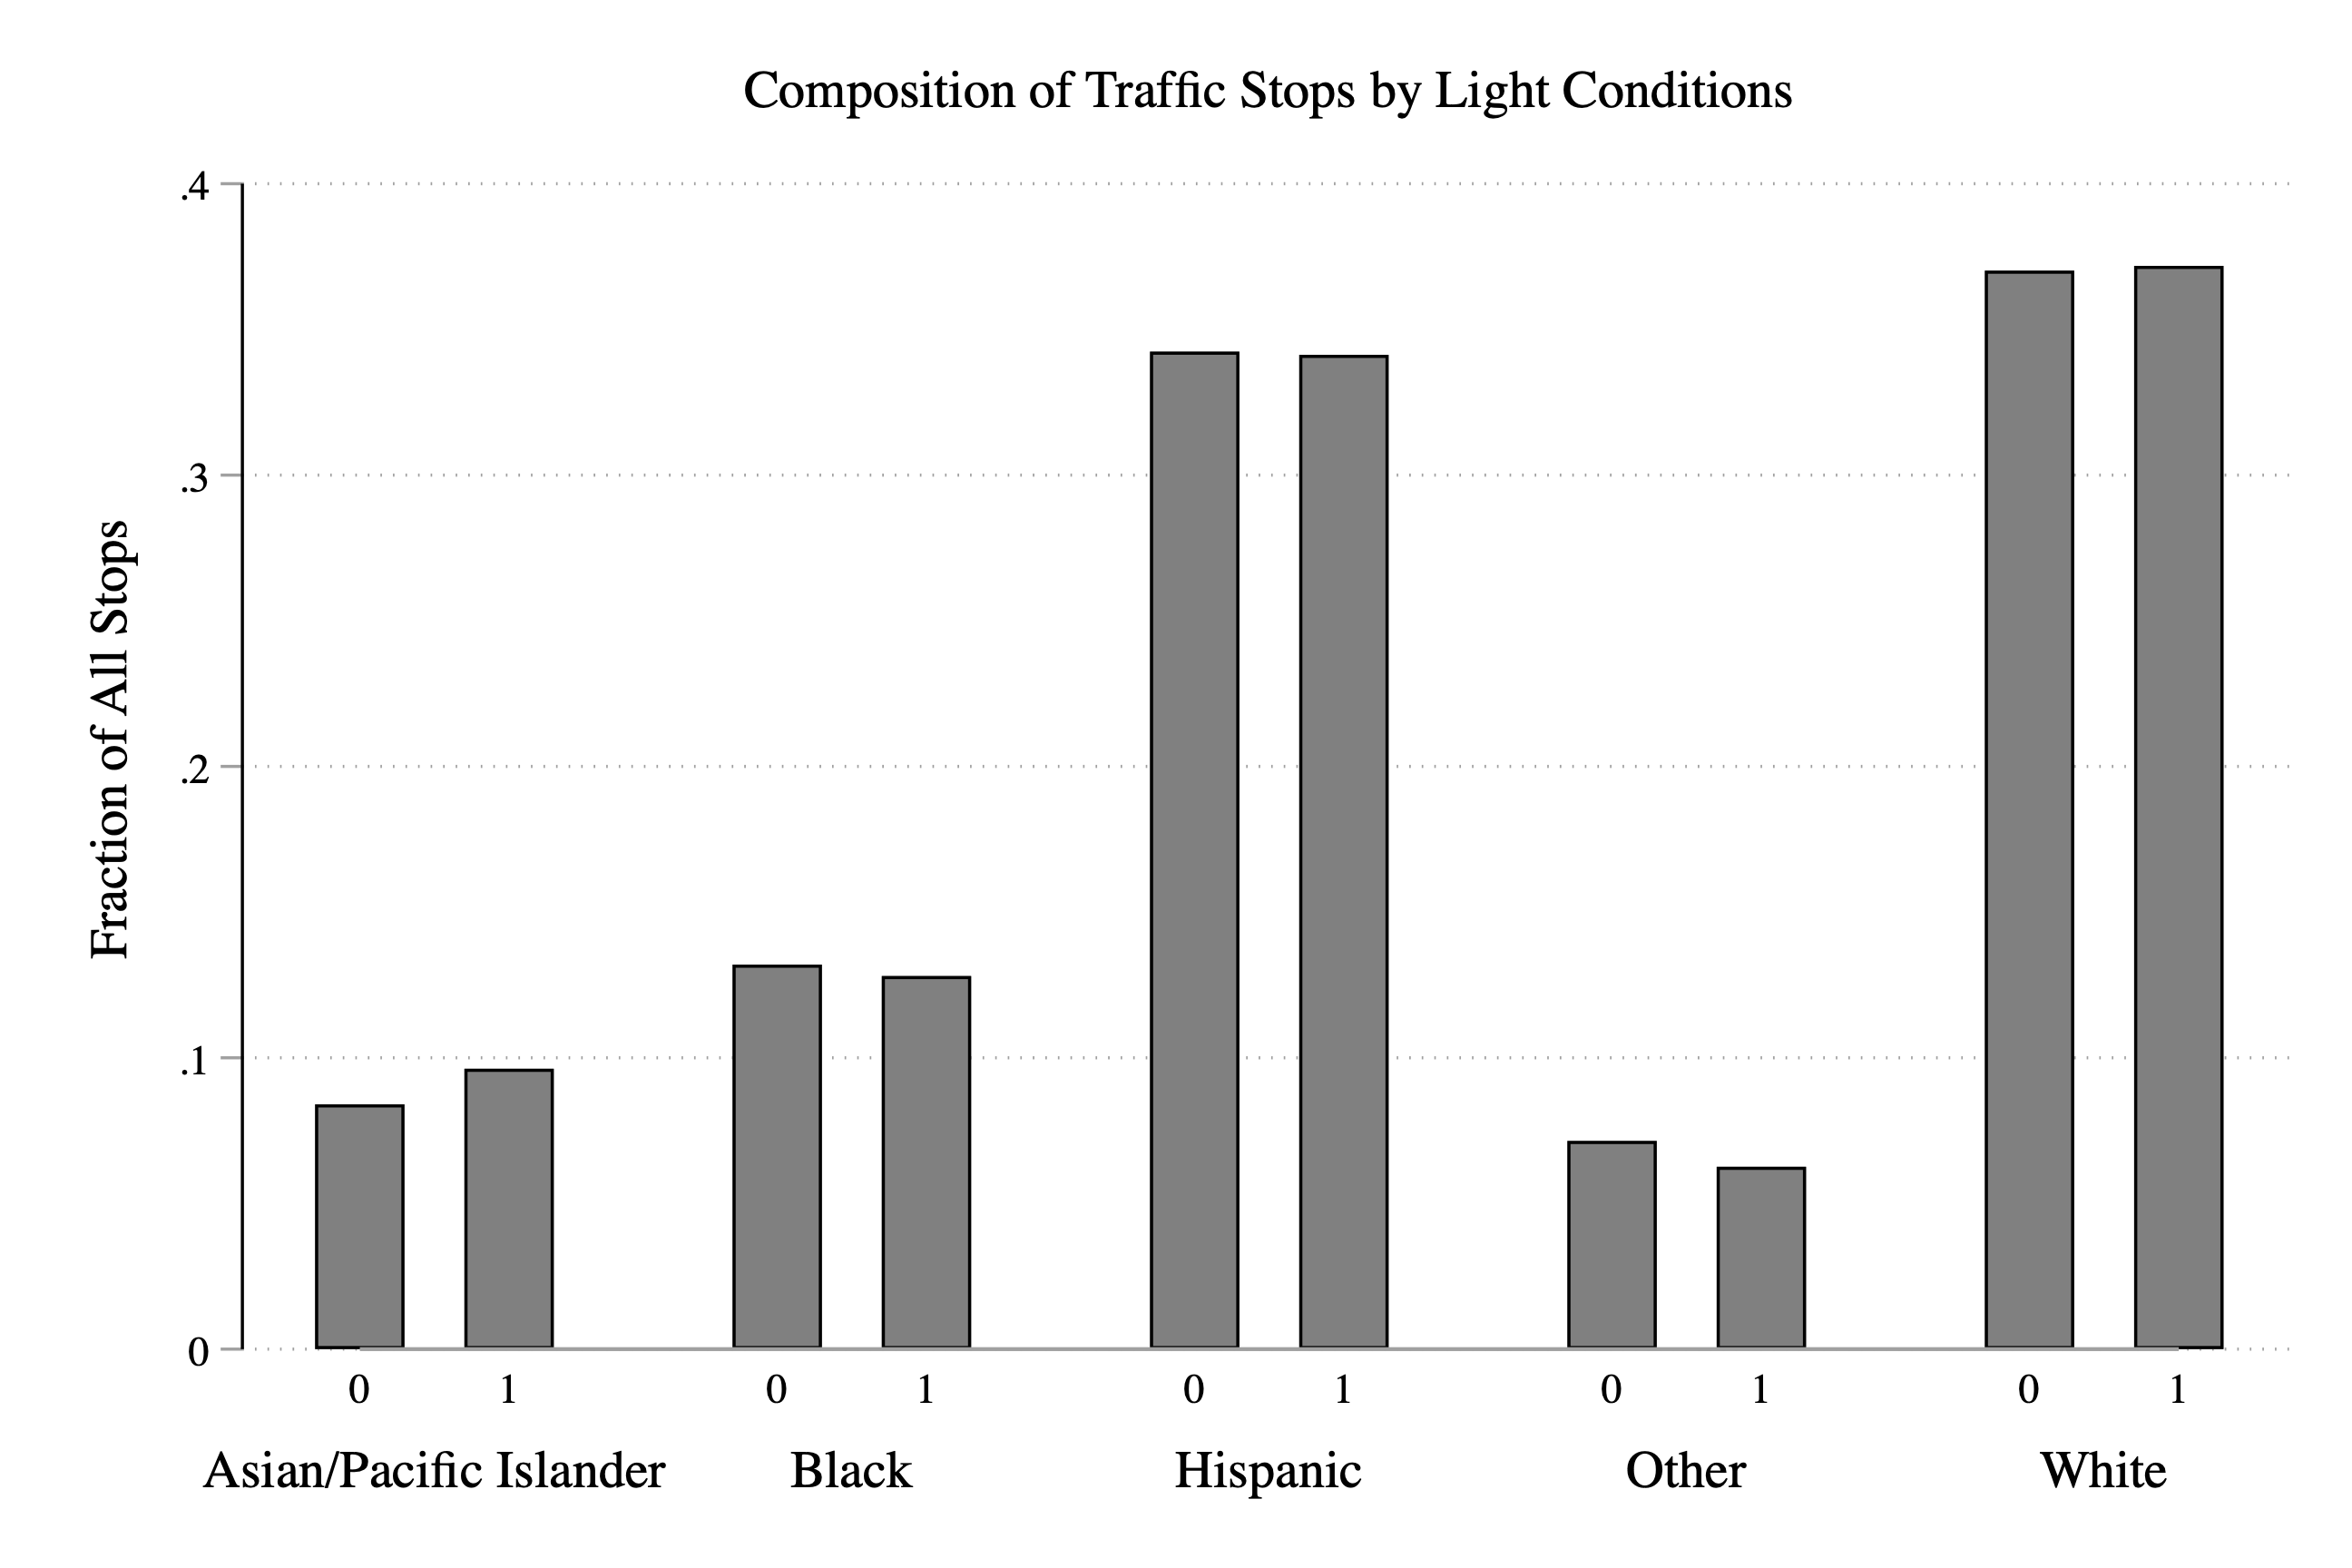
\includegraphics[width=0.65\linewidth]{images/03_bar2} 

}

\caption{Fraction of Stops by Race and Light Condition}\label{fig:bar2}
\end{figure}

Because we generated this data, we know \texttt{dark==0} represents daylight and \texttt{dark==1} represents darkness, but our reader won't. We need to relabel the zero to light and the 1 to dark so that a reader will understand what the graph represents. To do this, we can use the \texttt{relabel} option:

\begin{Shaded}
\begin{Highlighting}[]
\KeywordTok{graph} \BaseNTok{bar}\NormalTok{ fraction, }\CommentTok{///}
  \BaseNTok{over}\NormalTok{(dark,relabel(1 }\StringTok{"Light"}\NormalTok{ 2 }\StringTok{"Dark"}\NormalTok{)) }\BaseNTok{over}\NormalTok{(subject\_race) }\CommentTok{///}
  \BaseNTok{title}\NormalTok{(}\StringTok{"Composition of Traffic Stops by Light Conditions"}\NormalTok{) }\CommentTok{///}
  \BaseNTok{ytitle}\NormalTok{(}\StringTok{"Fraction of All Stops"}\NormalTok{) }
\end{Highlighting}
\end{Shaded}

\begin{figure}

{\centering 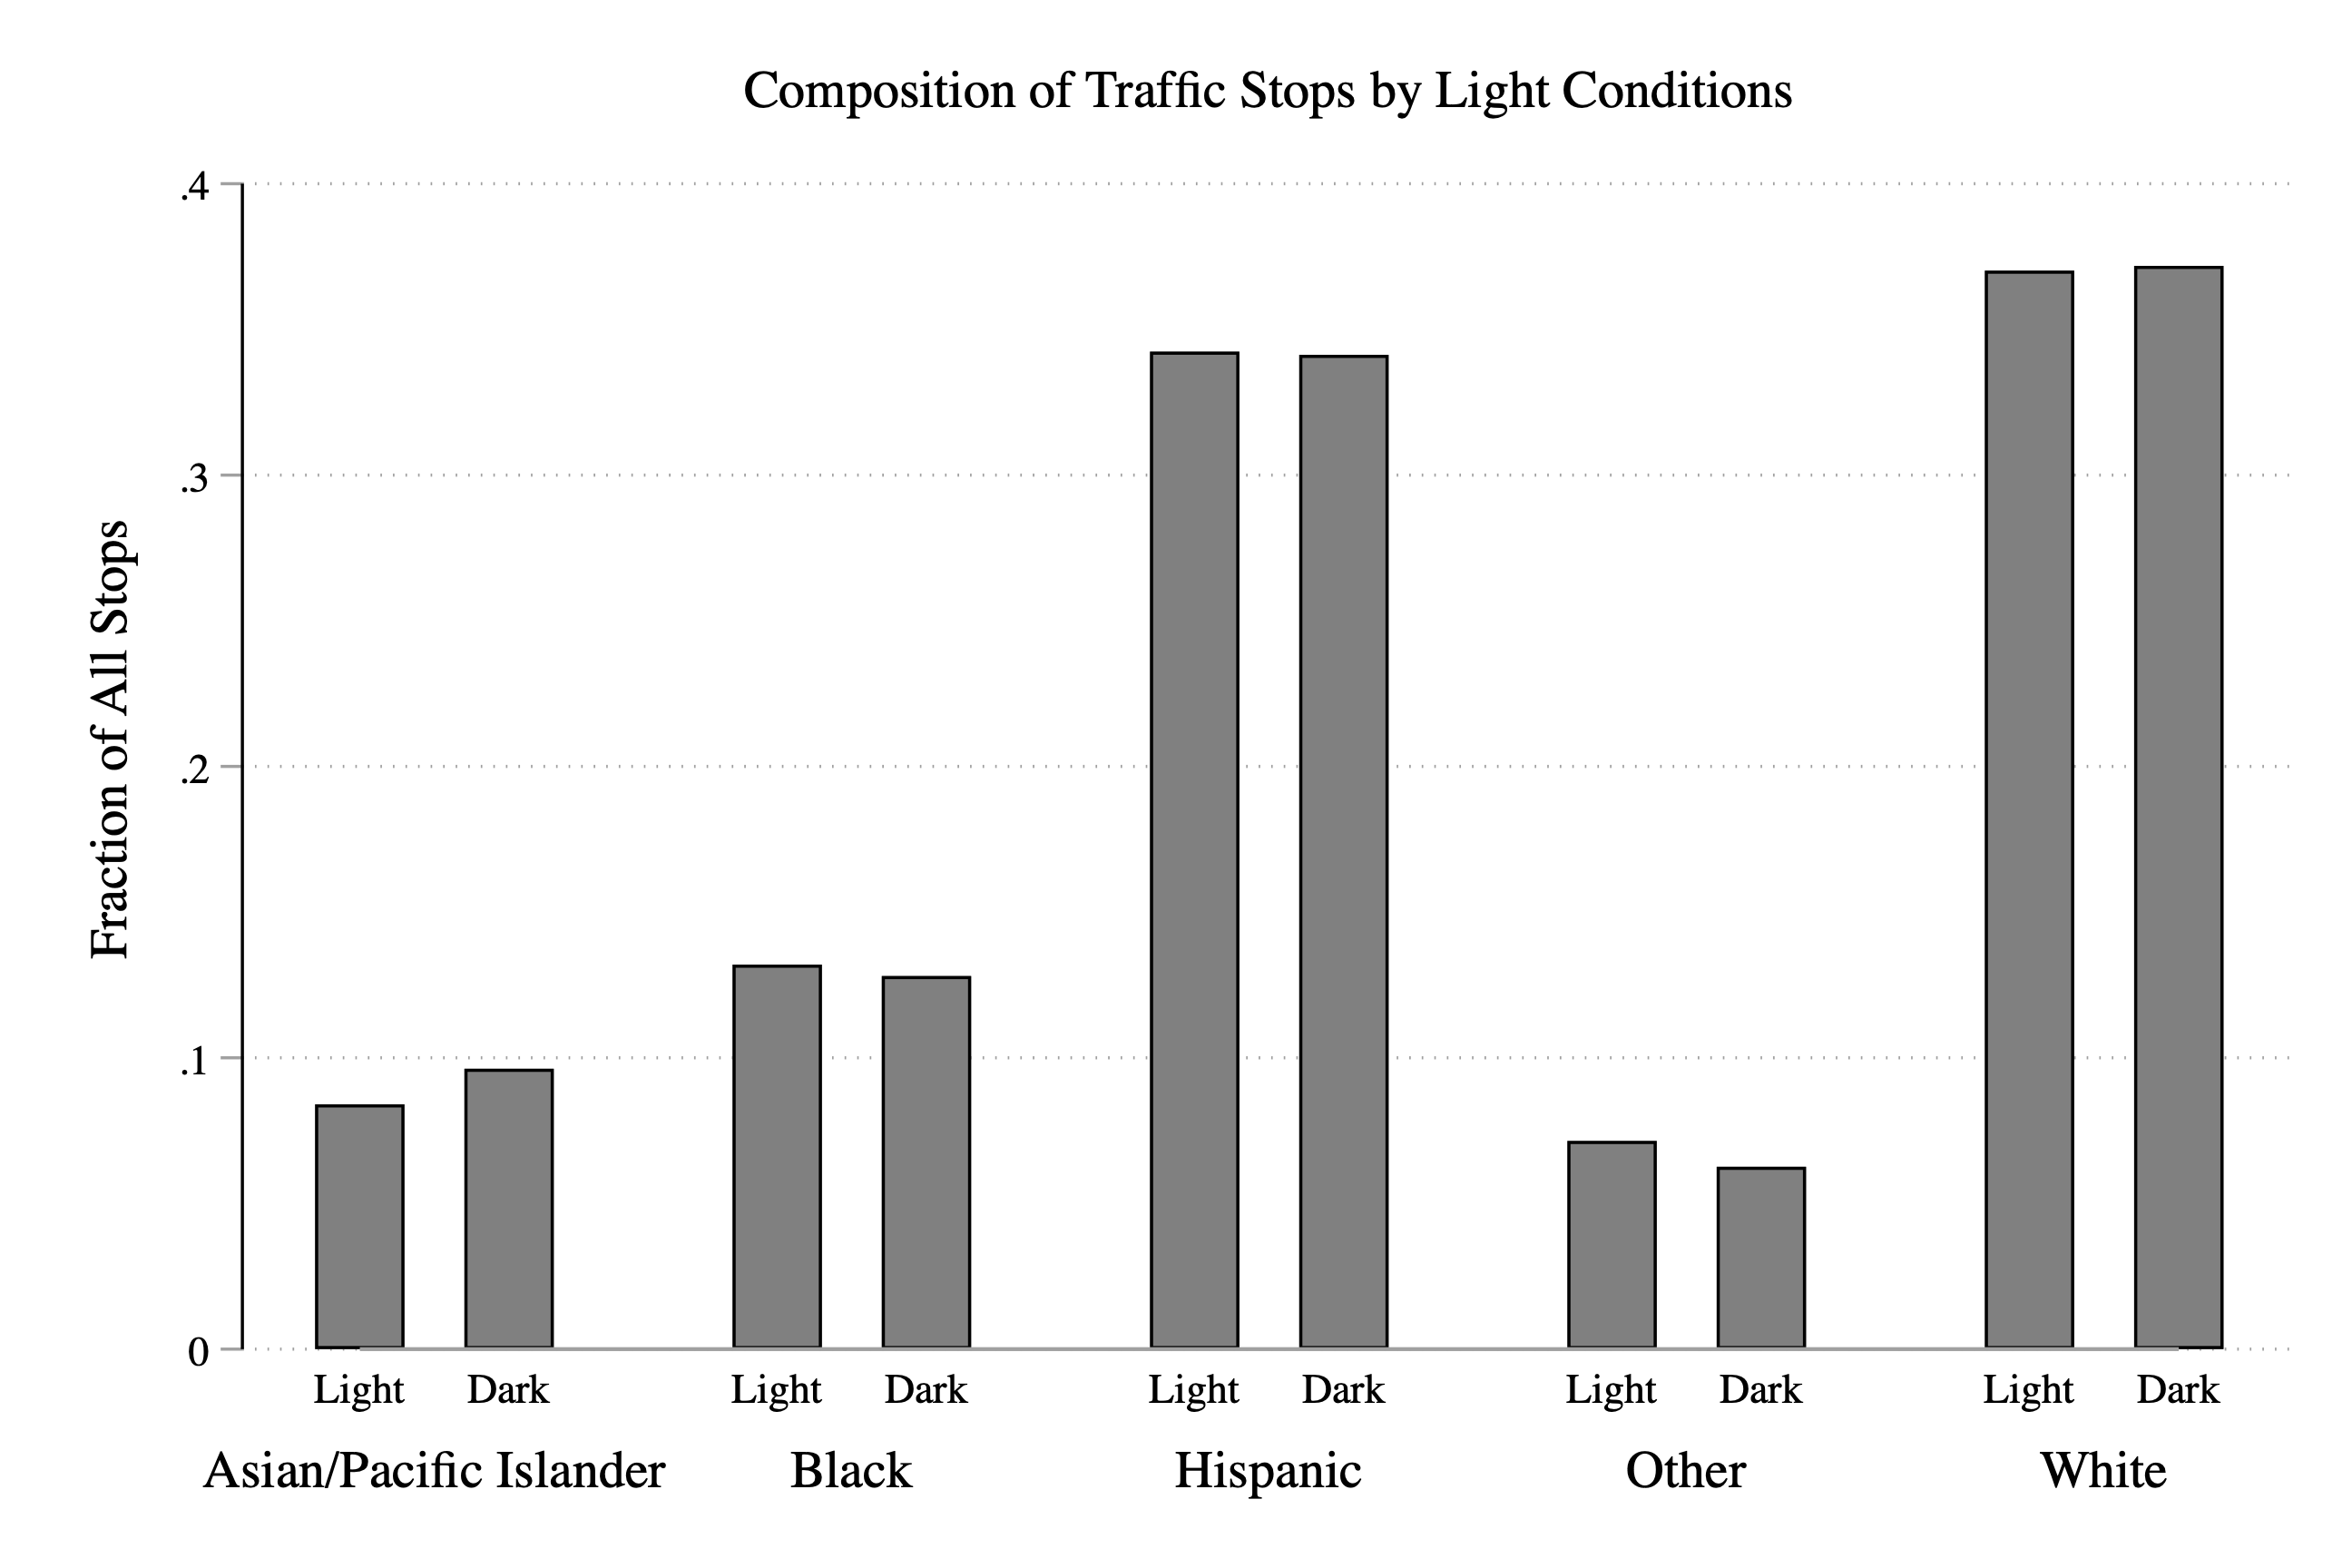
\includegraphics[width=0.65\linewidth]{images/03_bar3} 

}

\caption{Fraction of Stops by Race and Light Condition}\label{fig:bar3}
\end{figure}

Next, let's try to make our graph even easier to read. In practice, I don't expect you will need this next option too often, but it helps in our case. The option is \texttt{asyvars}, which treats the first \texttt{over()} group as a y-variable. What does this do in our case? Basically, it makes the \texttt{Light} and \texttt{Dark} labels appear in a legend instead of on the x-axis. This will make the graph look a little cleaner and easier to interpret quickly:

\begin{Shaded}
\begin{Highlighting}[]
\KeywordTok{graph} \BaseNTok{bar}\NormalTok{ fraction, asyvars }\CommentTok{///}
  \BaseNTok{over}\NormalTok{(dark,relabel(1 }\StringTok{"Light"}\NormalTok{ 2 }\StringTok{"Dark"}\NormalTok{)) }\BaseNTok{over}\NormalTok{(subject\_race) }\CommentTok{///}
  \BaseNTok{title}\NormalTok{(}\StringTok{"Composition of Traffic Stops by Light Conditions"}\NormalTok{) }\CommentTok{///}
  \BaseNTok{ytitle}\NormalTok{(}\StringTok{"Fraction of All Stops"}\NormalTok{) }
\end{Highlighting}
\end{Shaded}

\begin{figure}

{\centering 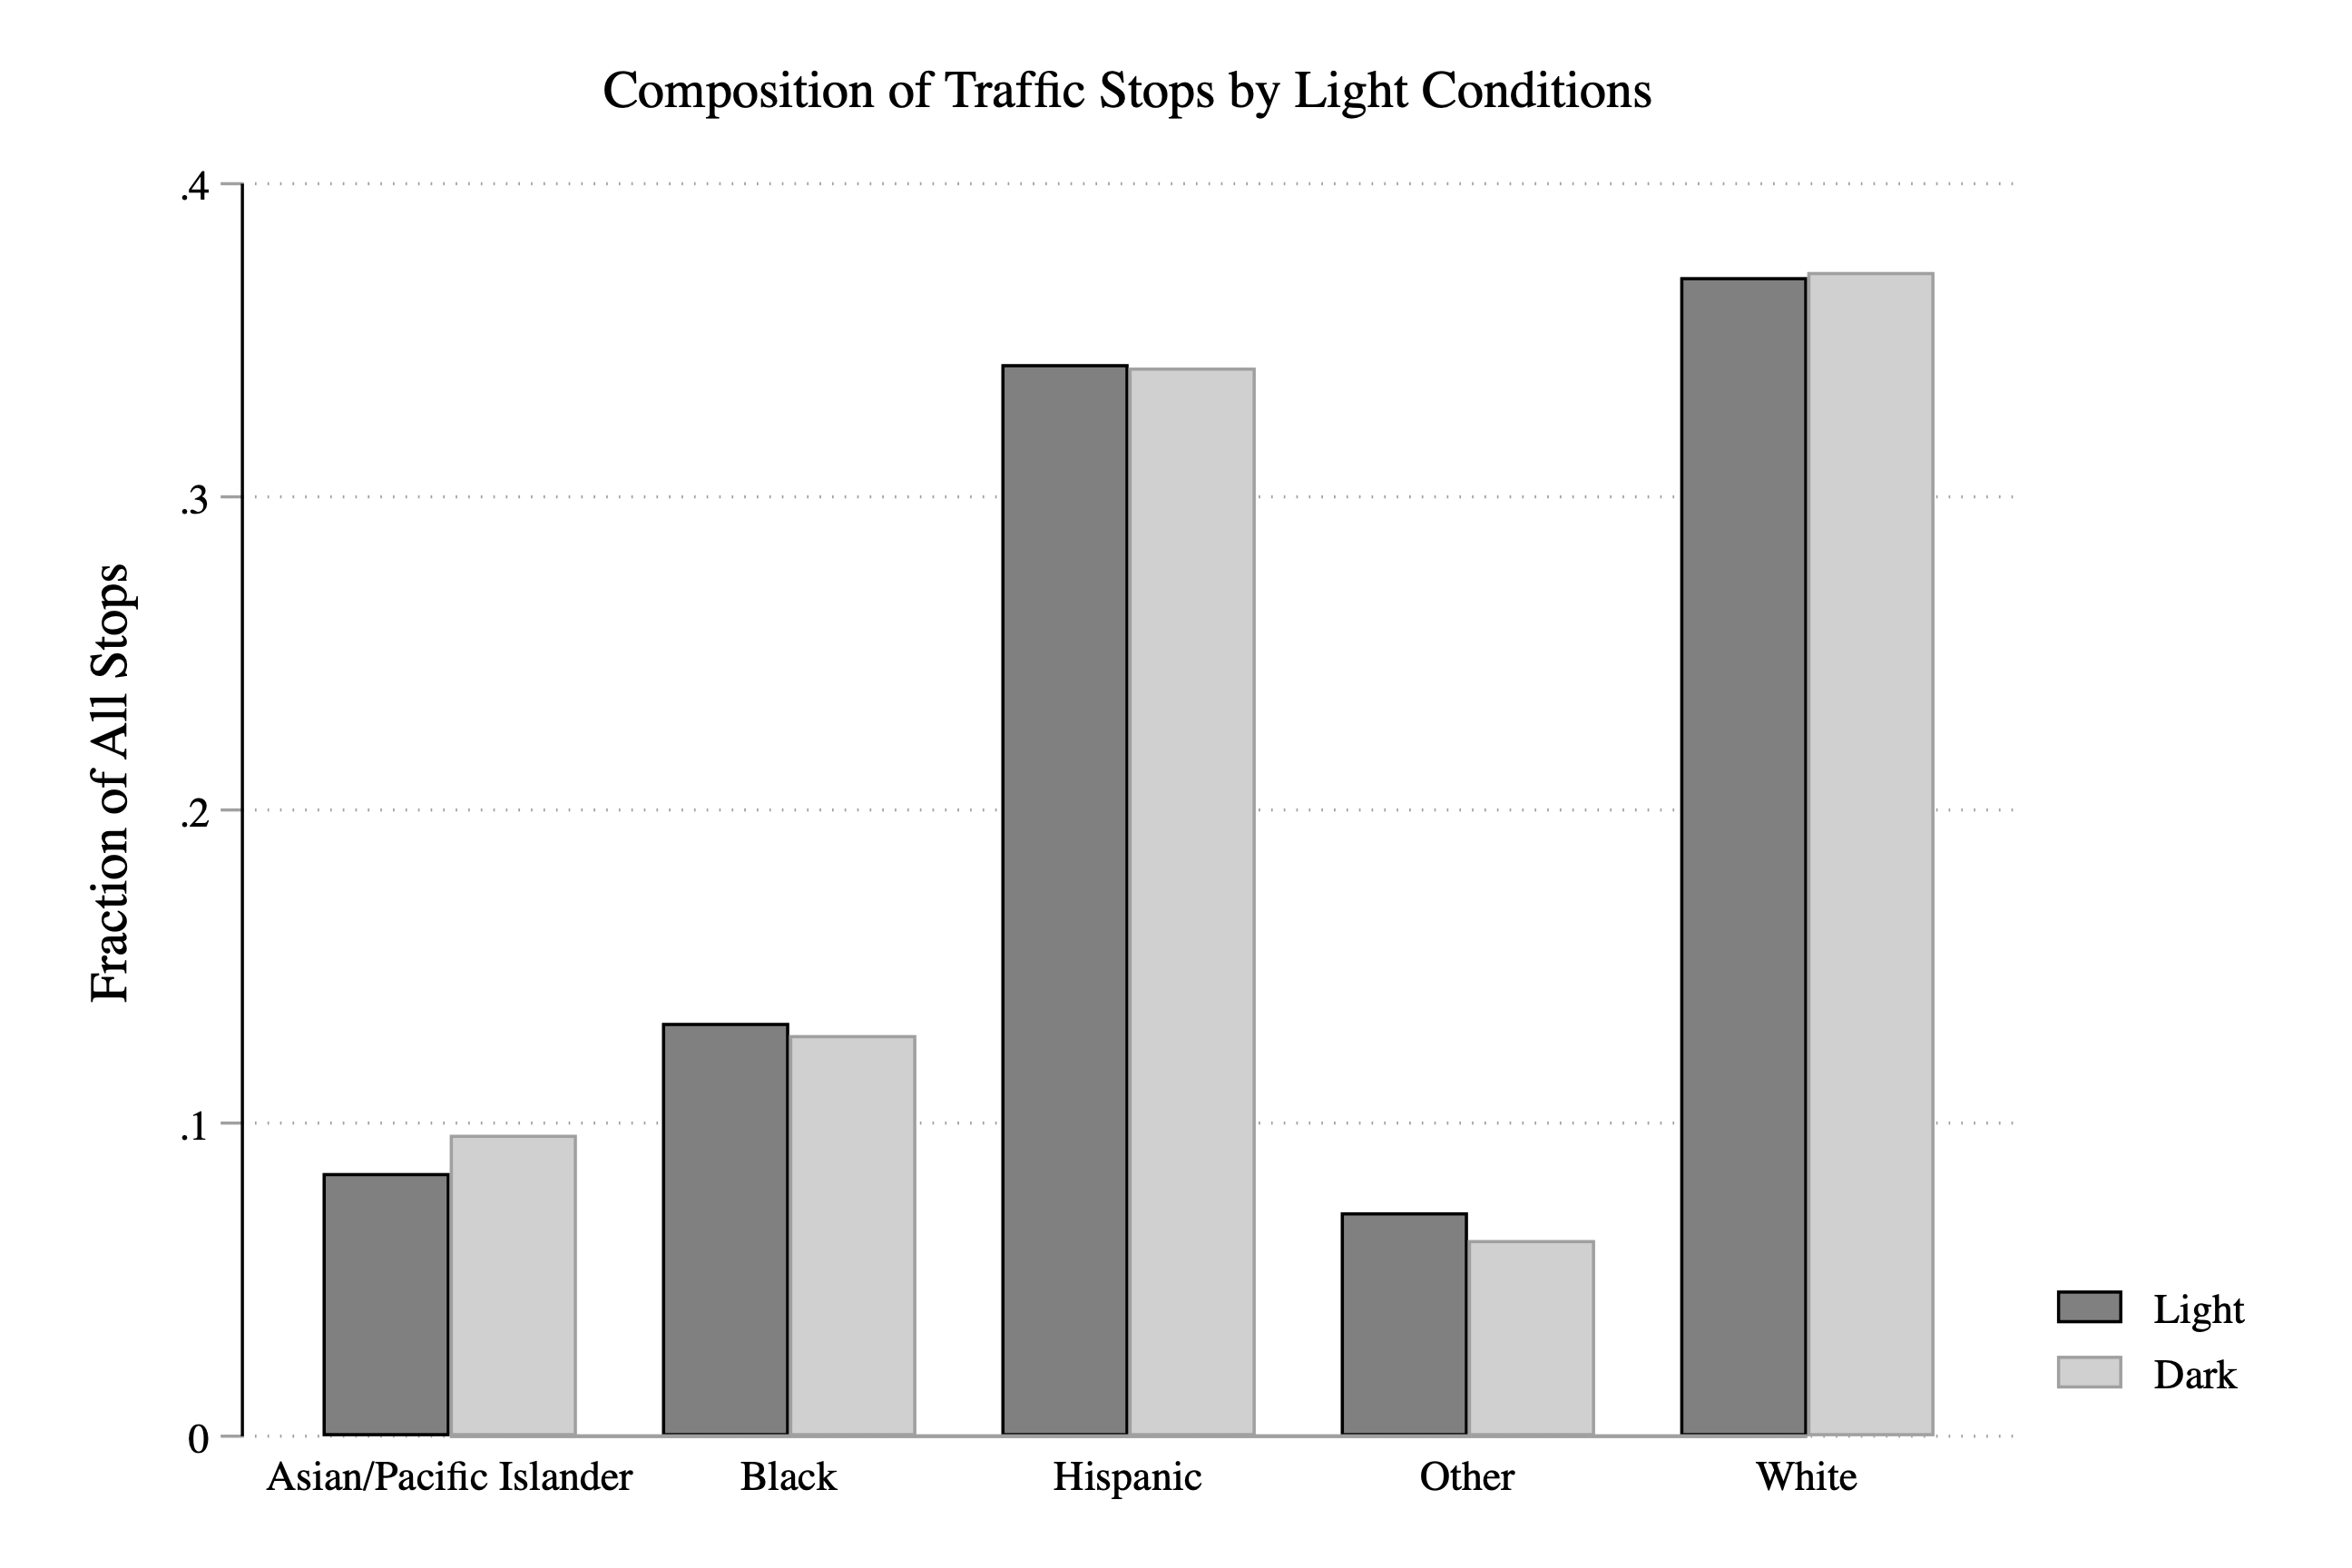
\includegraphics[width=0.65\linewidth]{images/03_bar4} 

}

\caption{Fraction of Stops by Race and Light Condition}\label{fig:bar4}
\end{figure}

The last step is to can change the colors of the bars. In the code below, \texttt{bar(1,\ fcolor(sky))} changes the \texttt{Light} bars to a sky blue. \texttt{bar(2,color(vermillion))} changes the \texttt{Dark} bars to vermillion.

\begin{Shaded}
\begin{Highlighting}[]
\KeywordTok{graph} \BaseNTok{bar}\NormalTok{ fraction, asyvars }\CommentTok{///}
  \BaseNTok{over}\NormalTok{(dark,relabel(1 }\StringTok{"Light"}\NormalTok{ 2 }\StringTok{"Dark"}\NormalTok{)) }\BaseNTok{over}\NormalTok{(subject\_race) }\CommentTok{///}
  \BaseNTok{title}\NormalTok{(}\StringTok{"Composition of Traffic Stops by Light Conditions"}\NormalTok{) }\CommentTok{///}
  \BaseNTok{ytitle}\NormalTok{(}\StringTok{"Fraction of All Stops"}\NormalTok{) }\CommentTok{///}
  \BaseNTok{bar}\NormalTok{(1, fcolor(sky)) }\CommentTok{///}
  \BaseNTok{bar}\NormalTok{(2, fcolor(vermillion))}
\end{Highlighting}
\end{Shaded}

\begin{figure}

{\centering 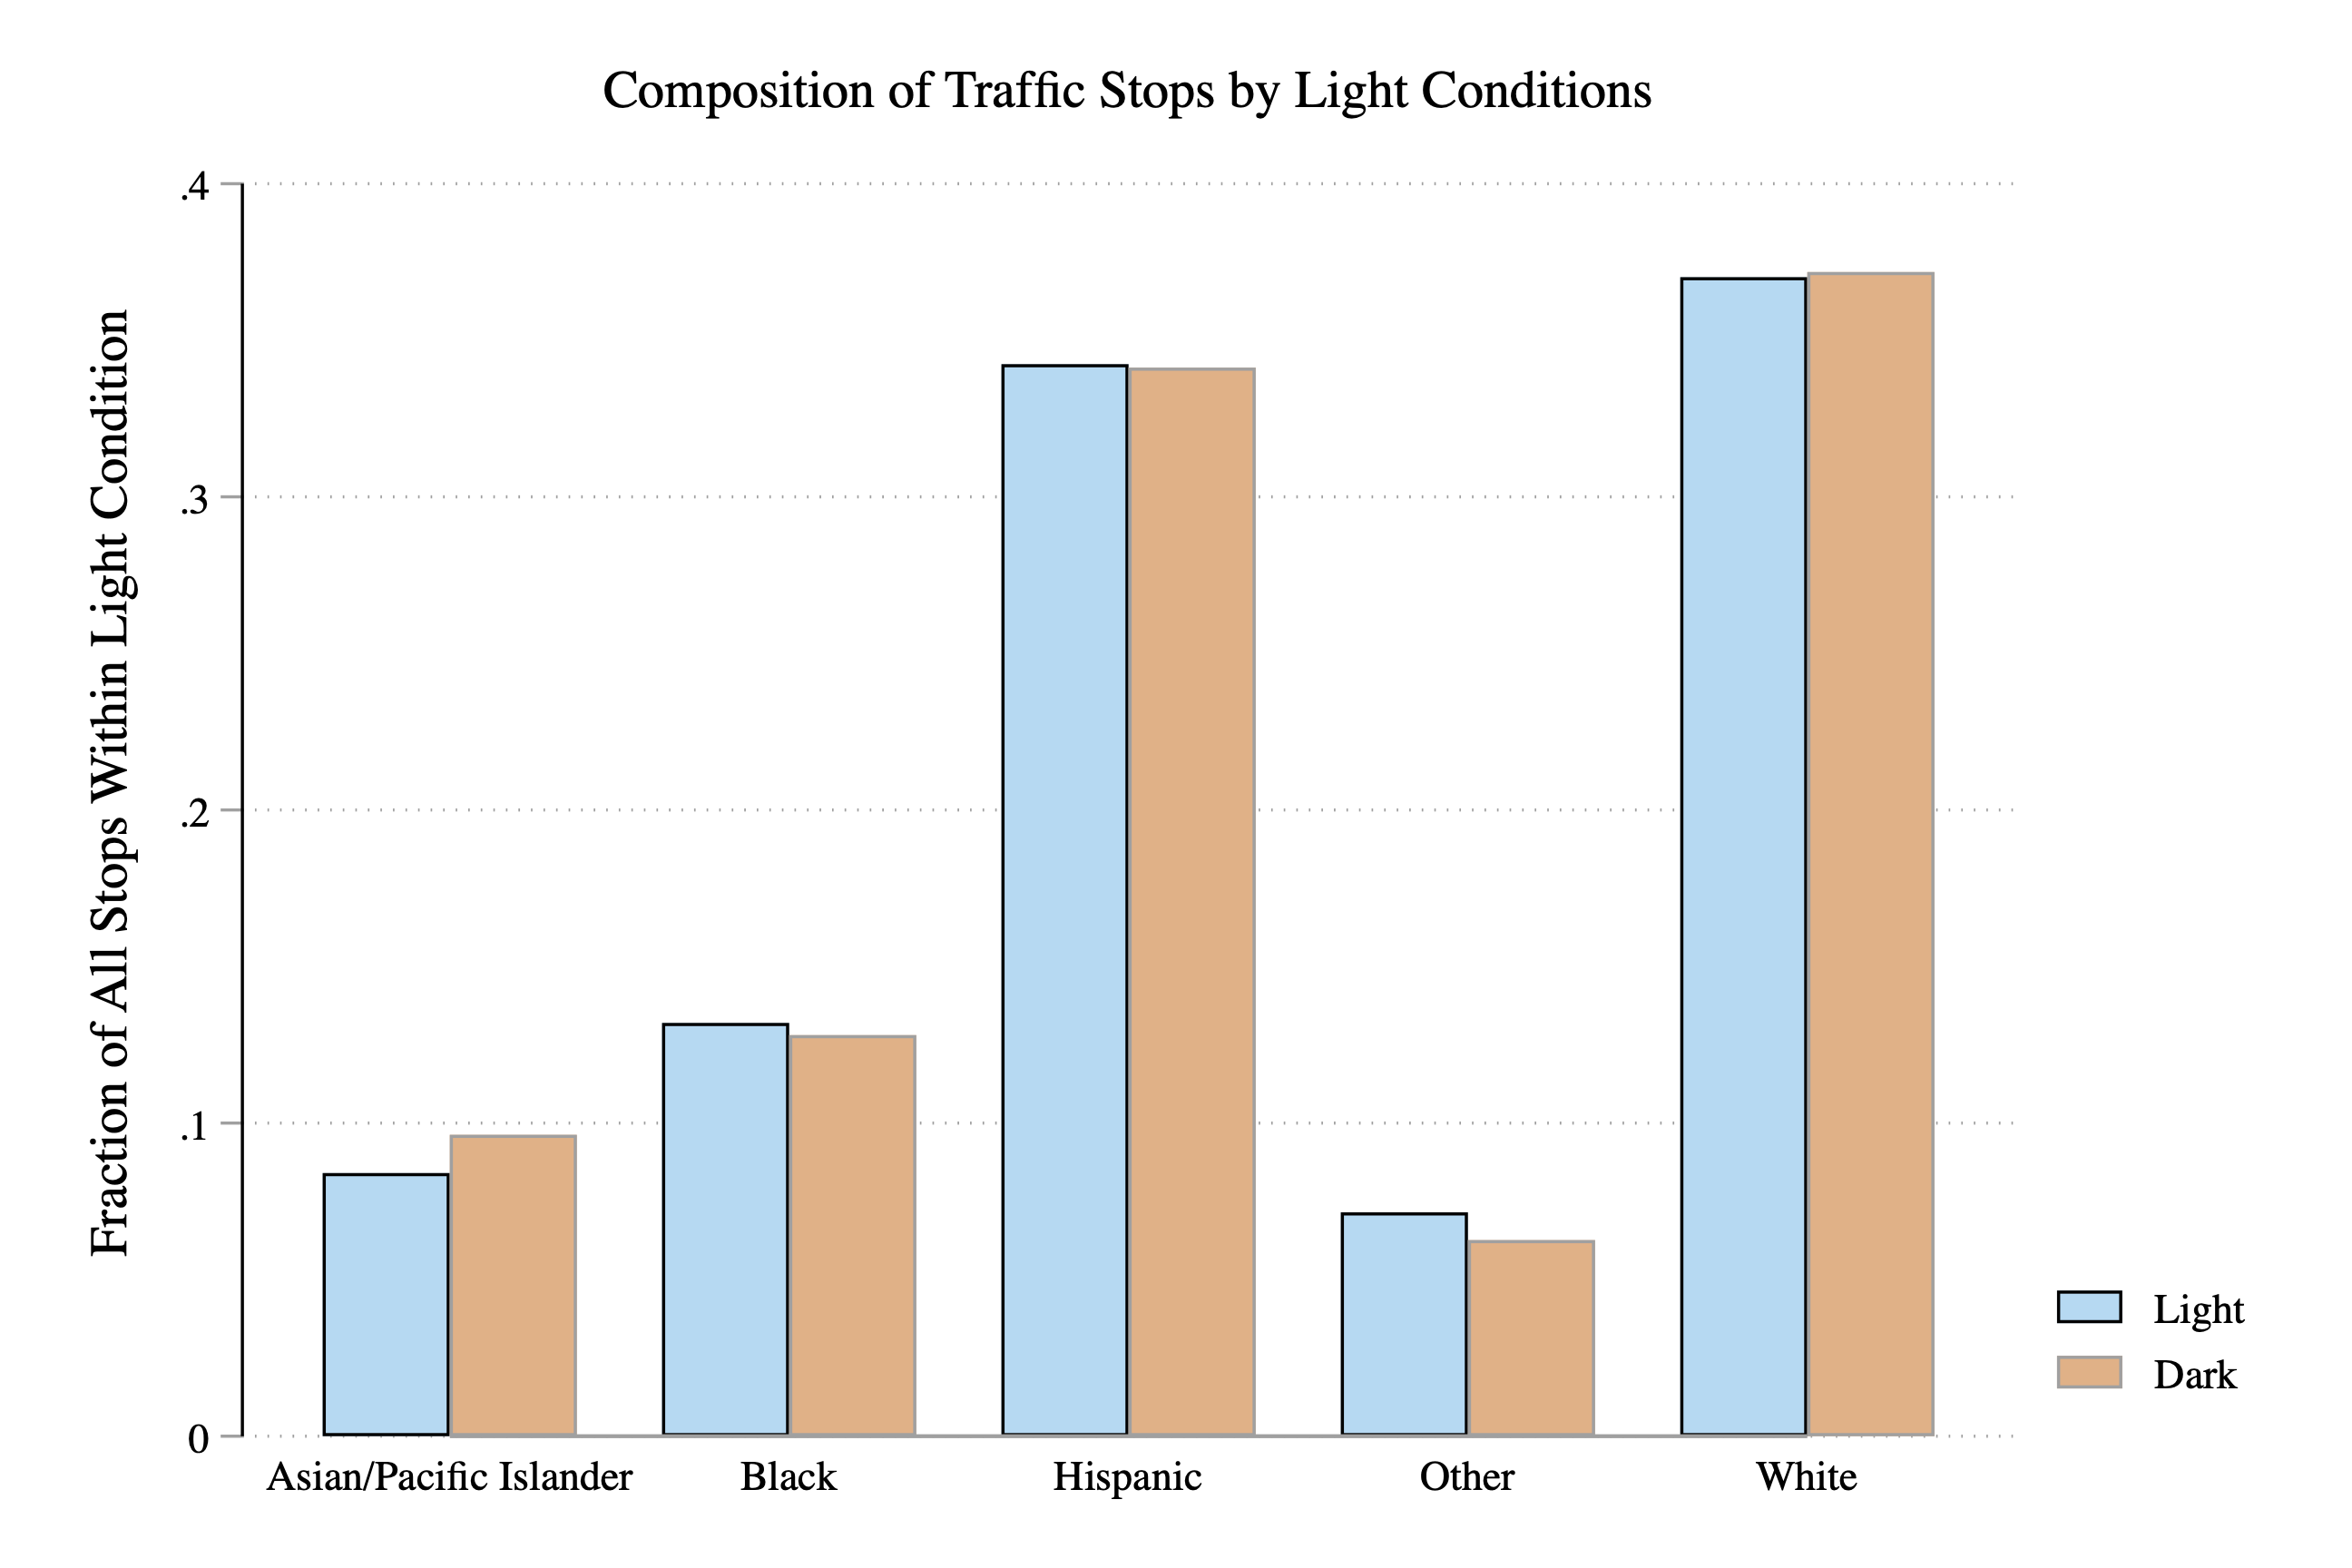
\includegraphics[width=0.65\linewidth]{images/03_bar5} 

}

\caption{Fraction of Stops by Race and Light Condition}\label{fig:bar5}
\end{figure}

So now let's spend a little time interpreting our main result. Overall, it appears that the fraction of stops for a given race does not depend dramatically on the light condition. We can see this in the graph by the fact that the blue and orange bars tend to be around the same height. If the orange bar (i.e.~\texttt{dark==1}) was dramatically lower for some races, then that would be evidence that police were targeting this race in the daylight.

Like any empirical design, the test has assumptions and limitations. It is not a fatal flaw that a given set of research has limitations. All research has limitations and it is important to think carefully about them. In the next section, we will discuss some of these limitations as well as feature some other factors that could be studied with the Stanford Open Policing Project data.

\section{Conclusion}\label{conclusion-1}

Let's discuss a few of the implicit assumptions in the veil of darkness test. First, we assumed driver race is unobservable after dusk. But what about artificial lighting, like street lamps? If in certain areas officers can detect race, then this method will underestimate level of discrimination. In other words, if driver race is observed in both sunlight and darkness, then the logic of the test as a method to identify discrimination no longer holds.

Another assumption is that driving behavior is the same before and after dark. What if minority drivers adjust their driving behavior because of potential racial profiling in daylight? Kalinowski, Ross, and Ross (2021)\citep{kalinowski2017endogenous} find evidence that this is true in certain areas.

This data has a lot of possibilities and we have explored only a small portion of it. In this final section let's think about a few more possible questions to explore.

First, we have focused on one place: San Diego. But we can look at how this test finds different results across different areas. If we find different results, we can ask why. What factors predict high levels of discriminatory behavior? Are there policies that could be used to reduce discriminatory behavior?

Second, we have focused on the initial decision to stop a driver. There could be discrimination at other stages of the stop. For example, are police officers more likely to search for contraband if the driver is a minority? This is something the researchers at the Stanford Open Policing Project have explored. Below is a figure from the SOPP website that shows search rates by race across different U.S.

\begin{figure}

{\centering 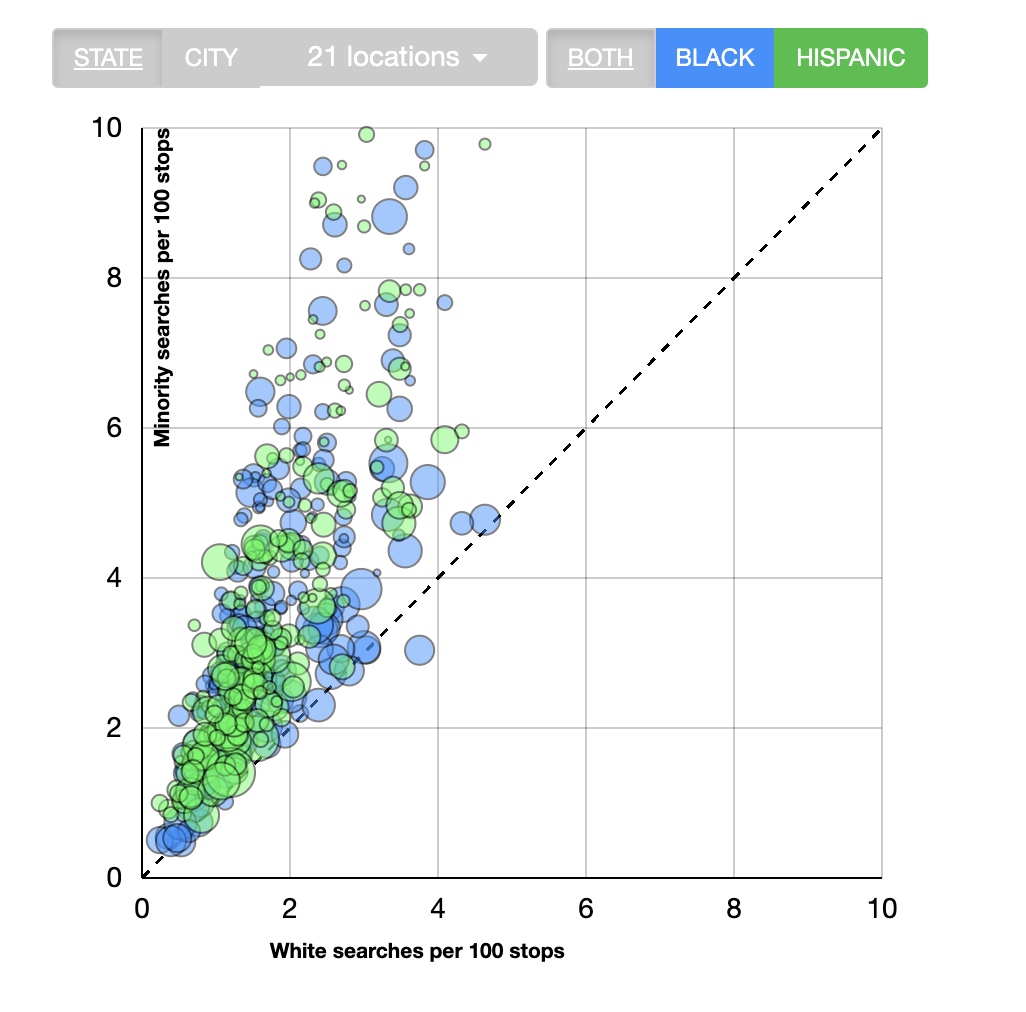
\includegraphics[width=0.65\linewidth]{images/03_search_rates} 

}

\caption{Disparities in Search Rates Across U.S. Cities}\label{fig:searchrates}
\end{figure}

As can be seen in Figure \ref{fig:searchrates}, the search rates tend to be higher for Black and Hispanic drivers across most cities in the U.S.

This still just scratches the surface of what can be done with this data! The main takeaway from this chapter: data can be a powerful tool that informs policy. The Stanford Open Policing Project is one effort to improve transparency in policing by making data publicly available to researchers and journalists.

\chapter{Classroom Technology}\label{classroom-technology}

\section{Disrupting Education Intro}\label{disrupting-education-intro}

Many developing countries have rapidly expanded access to education. However, not all places see measurable gains in learning. For example, in India, over 50 percent of students in grade 5 cannot read at a grade 2 level, despite enrollment rates around 95 percent (Pratham 2017)\citep{pratham2017}.

One hypothesis behind this puzzling fact is termed the mismatch hypothesis. If the curriculum is beyond a student's level of understanding, they may learn very little, even if attendance is high. In other words, there is a mismatch between the level of understanding and the curriculum being taught. In Muralidharan, Singh and Ganimiam (2019)\citep{msg2019disrupting}, the authors study whether a technology that aims to ``Teach at the Right Level'' can be used to improve learning outcomes. This is an important question: we need to find interventions that work! It is not necessarily true that more investment in education results in better outcomes if we are investing in the wrong things.

The technology the authors study is called Mindspark. Mindspark is a computer software that provides learning materials that are appropriate for a student's understanding level. It does this by using information on what questions a student gets right vs.~wrong. The level of material only increases in difficulty once the student has learned the previous concepts. Mindspark centers provide 6-day-a-week instruction for 90 minutes (45 minutes with Mindspark, 45 minutes with a teaching assistant). The question in Muralidharan, Singh and Ganimiam (2019) is: does this program improve learning outcomes?

To answer this question, the authors recruited participants from low-income neighborhoods in Delhi. At demonstration sessions for Mindspark, parents were introduced to the program. All participants interested in participating needed to fill out a baseline assessment. Then, parents were told that about half of the participants would receive a voucher that waived tuition for the Mindspark program (participants were chosen by lottery). Students not chosen by lottery were told they would obtain free access to the centers after February 2016 (after the experiment had concluded). The result is 619 participants, 305 in the control (i.e.~no access to Mindspark) and 314 in the treatment (access to Mindspark)

To begin, let's load the dataset \texttt{mindspark\_data.dta}

\begin{Shaded}
\begin{Highlighting}[]
\NormalTok{cd }\StringTok{"/Users/davidarnold/Dropbox/Teaching/EP5/online/04\_week/data"}
\KeywordTok{use}\NormalTok{ mindspark\_data.dta, }\KeywordTok{replace}
\NormalTok{file gapminder.dta }\KeywordTok{not}\NormalTok{ Stata }\KeywordTok{format}
\FunctionTok{r}\NormalTok{(610);}


\NormalTok{/Users/davidarnold/Dropbox/Teaching/EP5/online/04\_week/}\KeywordTok{data}
\end{Highlighting}
\end{Shaded}

As usual, let's begin by describing the dataset

\begin{figure}

{\centering 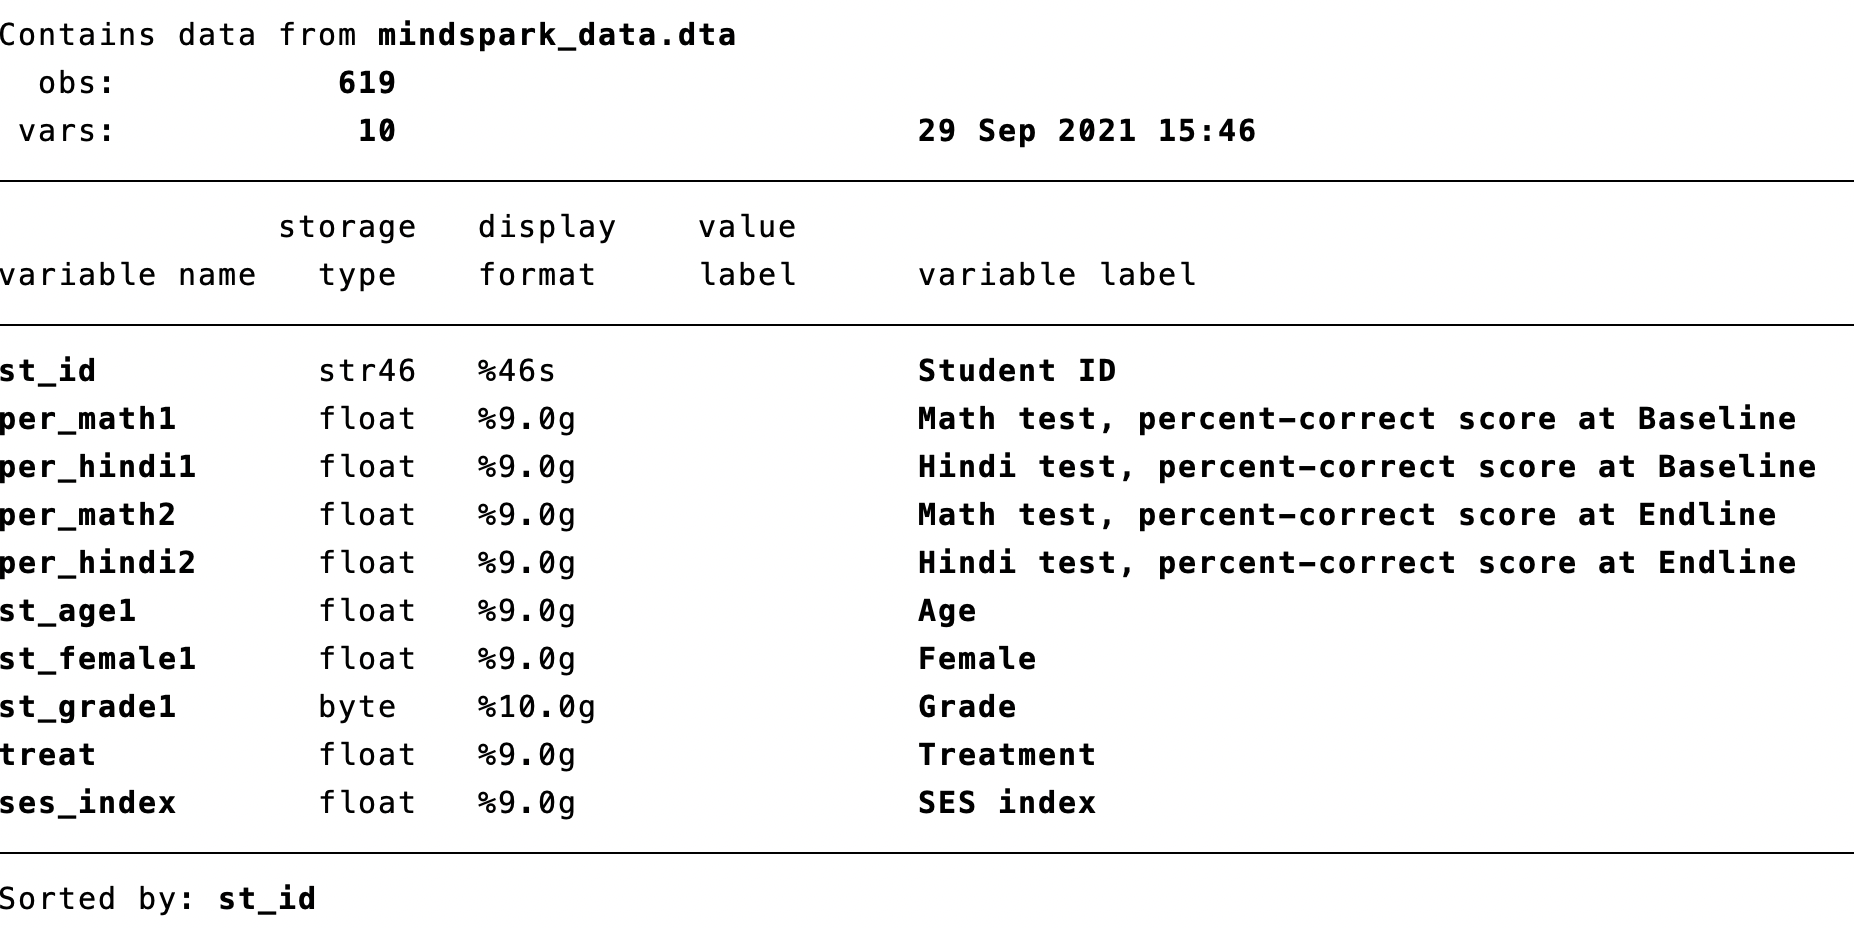
\includegraphics[width=0.9\linewidth]{images/04_describe} 

}

\caption{Describing the Mindspark Data}\label{fig:msdescribe}
\end{figure}

This is a subset of all variables in Muralidharan, Singh, and Ganimian (2019). We are interested in how being treated impacts learning outcomes. We have information about Math and Hindi tests at both the baseline and endline. Baseline means the test was taken before any student has been offered free Mindspark. Endline means the test was taken after the treated students had received Mindspark and had been using the software for several months. To start, let's summarize these variables to get a sense of average test scores as well as the variation in test scores at baseline.

\begin{Shaded}
\begin{Highlighting}[]
\KeywordTok{sum}\NormalTok{ per\_math1}
\KeywordTok{sum}\NormalTok{ per\_hindi1}
\end{Highlighting}
\end{Shaded}

\begin{verbatim}
file gapminder.dta not Stata format
r(610);


no variables defined
r(111);

r(111);
\end{verbatim}

At the baseline, the average score on the math test was 0.318. This indicates that on average across students, the average score was 31.8 percent on the math test. For the Hindi test, the average was a bit higher at 0.428. Now let's look at endline scores.

\begin{Shaded}
\begin{Highlighting}[]
\KeywordTok{sum}\NormalTok{ per\_math2}
\KeywordTok{sum}\NormalTok{ per\_hindi2}
\end{Highlighting}
\end{Shaded}

\begin{verbatim}
file gapminder.dta not Stata format
r(610);


no variables defined
r(111);

r(111);
\end{verbatim}

At endline, scores are higher. The average math score has increased to 0.503 and the average Hindi score has increased to 0.552. Our ultimate goal, however, is to understand how test scores change depending on whether you are given access to Mindspark. In other words, do test scores at endline depend on whether \texttt{treat==1} or \texttt{treat==0}? Before we start analyzing the data, however, we are going to learn a new statistical technique: \textbf{regression}.

\section{Linear Regression (Theory)}\label{linear-regression-theory}

Linear regression estimates a linear relationship between variables. Before getting to the estimation part, let's first review linear equations. A linear equation is any equation that can be written in the following form

\[
y=mx+b
\]

Where \(m\) is the slope and \(b\) is the intercept. For example, there is a linear relationship between degrees in Celsius (C) and degrees in Fahrenheit (F)

\[
F= 1.8 \cdot C + 32
\]

\begin{figure}

{\centering 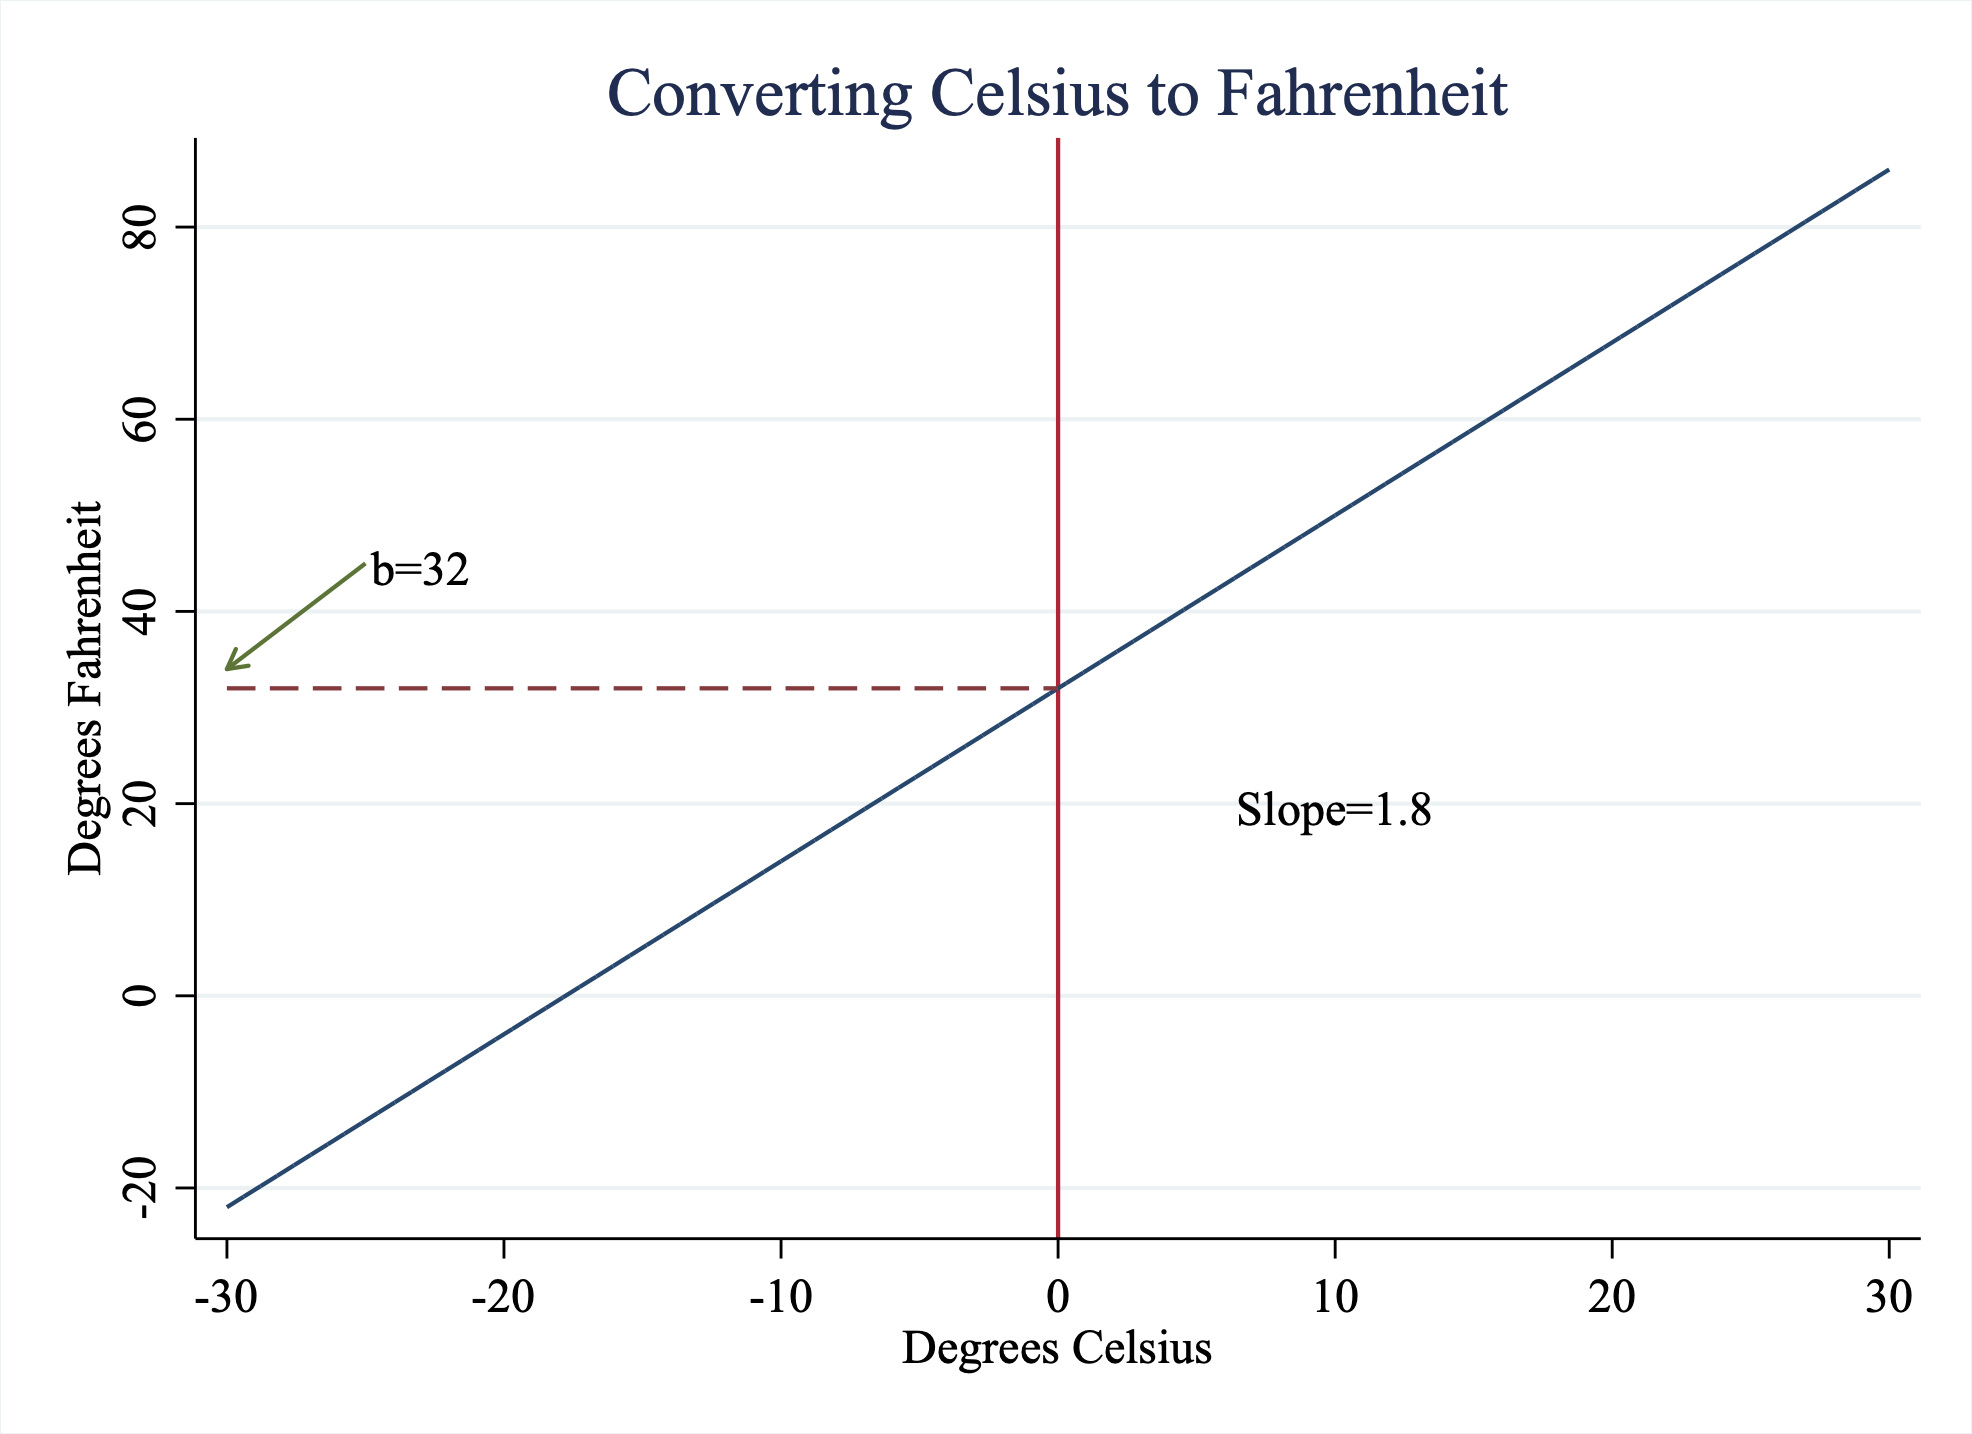
\includegraphics[width=0.9\linewidth]{images/04_ctof} 

}

\caption{Converting Celsius to Fahrenheit}\label{fig:ctof}
\end{figure}

In this example, there is a direct linear relationship between these two variables, Celsius and Fahrenheit. Often in the social sciences, we are interested in \textbf{estimating} the relationship between two variables. How much does education increase income? Does precipitation impact voter participation? One way to understand how two variables are related is through estimating linear relationships. \textbf{Linear Regression} is a way to estimate linear relationships between one or more variables

We want to model some outcome of individuals \(Y_i\) as a function of some explanatory variable of the individual \(X_i\) (in math: \(Y_i=f(X_i)\)). \(Y_i\) is often referred to as the dependent variable (or outcome variable). \(X_i\) is often referred to as the independent variable (or explanatory variable). If we assume the function \(f(X_i)\) is linear, then we can write this model as

\[
Y_i = \beta_0 + \beta_1 \cdot X_i + \varepsilon_i \nonumber
\]

Imagine we hypothesize that students who watch too much TV the night before a test perform worse. Then we want to understand if test scores (our outcome variable \(Y_i\)) is related to hours of TV watched (our explanatory variable \(X_i\)). We could posit a linear relationship between the two

\[
\text{Test Score}_i = \beta_0 + \beta_1 \cdot \text{Hours Watched TV}_i + \varepsilon_i 
\]

The parameters of the model are the parameters we are estimating. In a linear regression model, there are two parameters we need to estimate: \(\beta_0\) and \(\beta_1\) as the parameters of the model. We use ``hats'' to denote the estimates of these parameters. \(\hat{\beta}_0\) is the estimate of the intercept. \(\hat{\beta}_1\) is the estimate of the slope coefficient. We choose \(\hat{\beta}_0\) and \(\hat{\beta}_1\) to construct a regression line that best fits our data.

But what does best fit actually mean? We choose \(\hat{\beta}_0\) and \(\hat{\beta}_1\) to minimize the sum of squared errors (\(\sum \varepsilon_i^2\)). Choosing the parameters to minimize the sum of squared errors is referred to as \textbf{Ordinary Least Squares} and is commonly simply referred to as linear regression.

How do we go about finding the best fit? Let's consider estimating the relationship between the two variables below in Figure \ref{fig:reg2}. On the horizontal axis, we have hours spent watching TV, while on the vertical axis, we have how the student performed on the test. In this example, we have only four data points.

\begin{figure}

{\centering 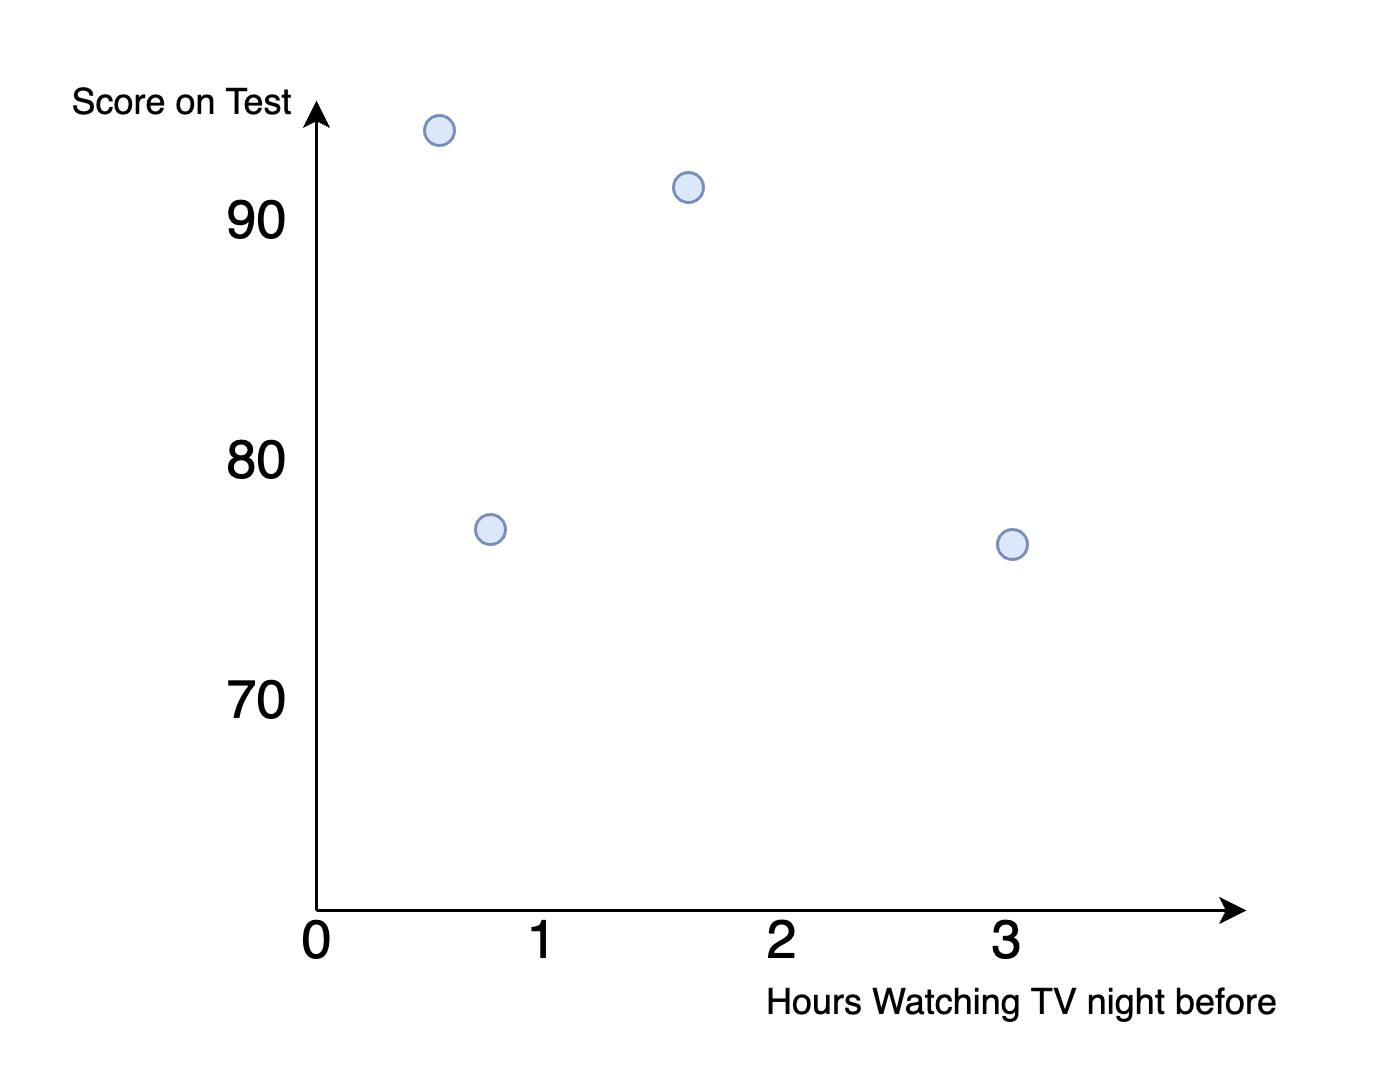
\includegraphics[width=0.9\linewidth]{images/04_reg2} 

}

\caption{Hypothetical Dataset: Finding the Best Fit Line}\label{fig:hypreg2}
\end{figure}

Let's draw a line and then assess whether the fit is good or bad. Consider the line in Figure \ref{fig:hypreg3}.

\begin{figure}

{\centering 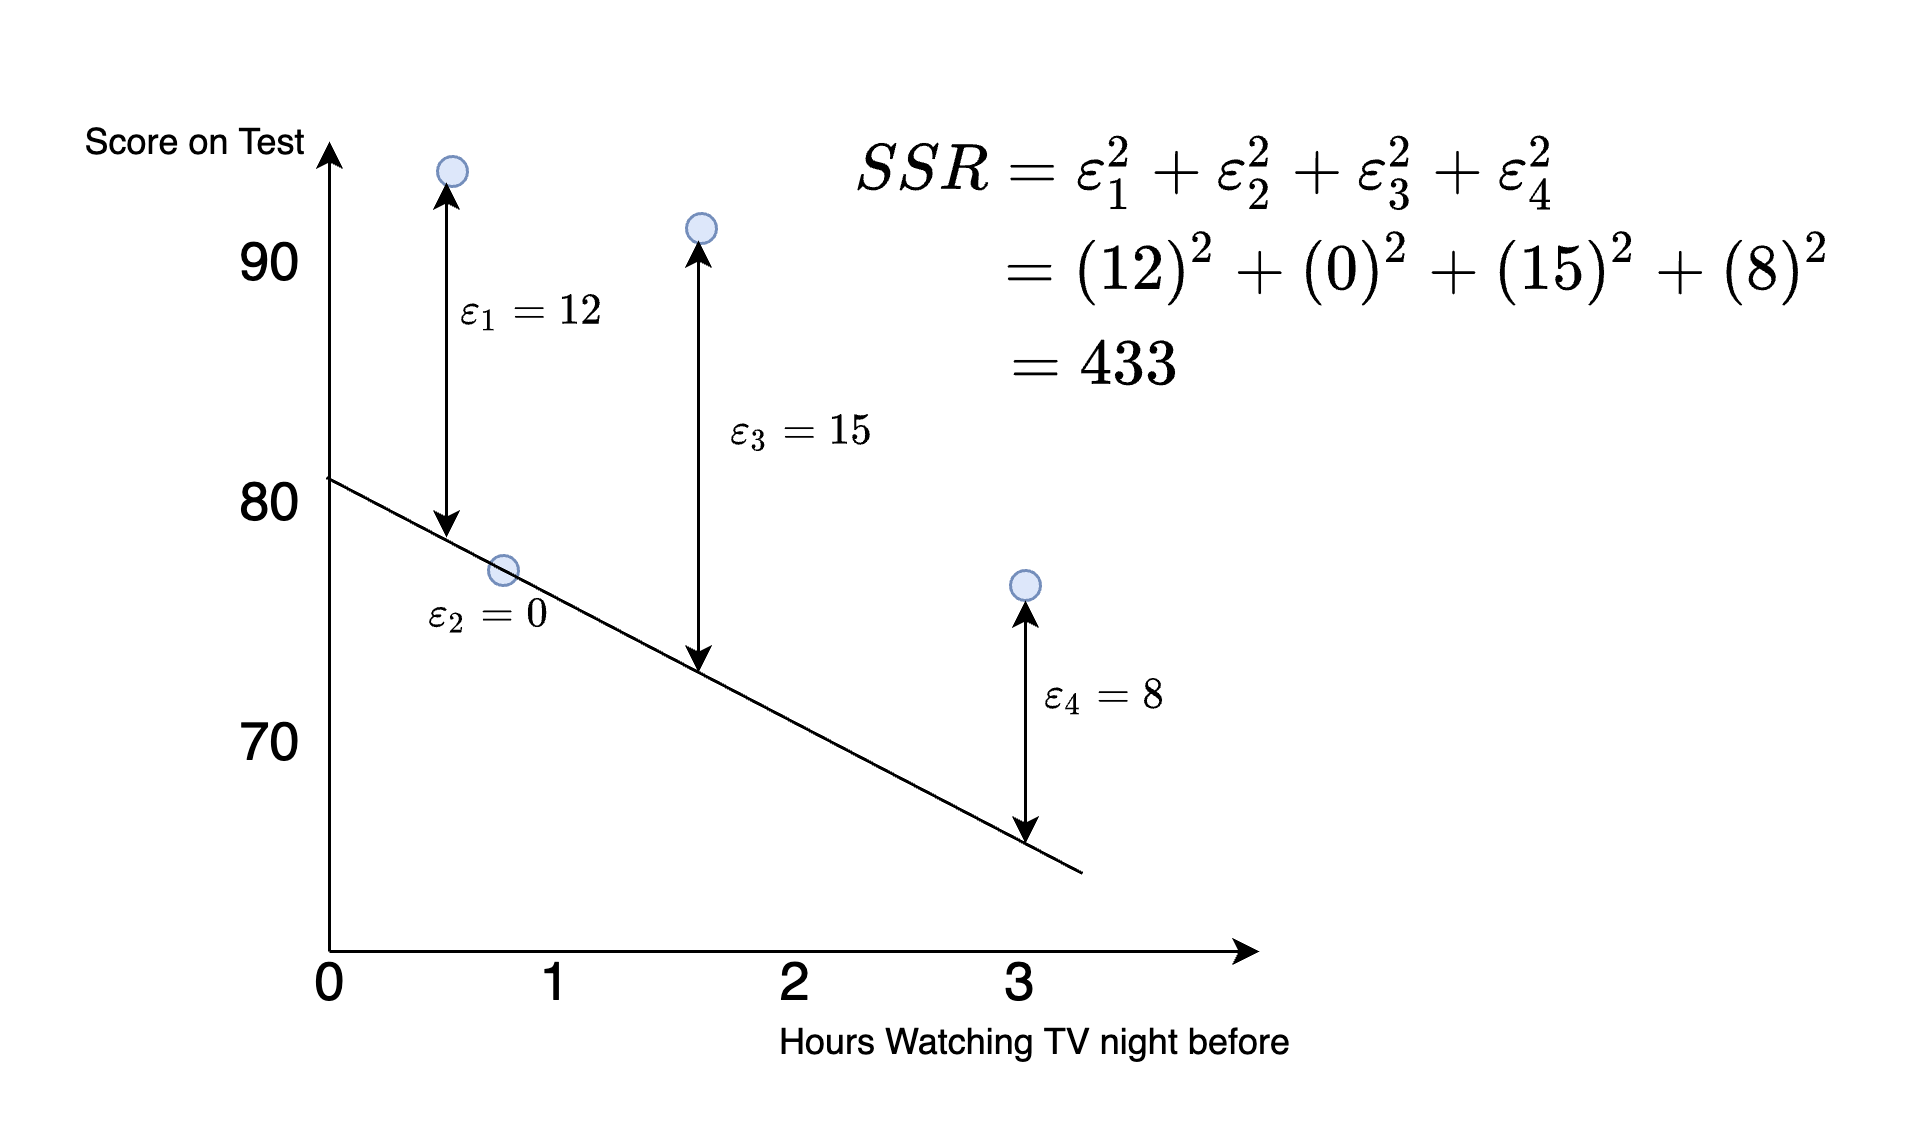
\includegraphics[width=0.9\linewidth]{images/04_reg4} 

}

\caption{Hypothetical Dataset: Finding the Best Fit Line}\label{fig:hypreg3}
\end{figure}

How well does this line fit? To measure this we take the difference between the line and the actual values, which is known as the residual. Some residuals are negative (meaning the actual value is less than that predicted based on our line), while others are positive (meaning the actual value is greater than that predicted based on our line). In terms of ``fit'' we don't care about whether the error is positive or negative, which is why when we assess fit we first ``square'' the residuals. The square of all residuals will then be a positive number, with larger positive numbers indicating higher error.

To construct one number that tells us how well the line fits the data we construct the sum of squared residuals. In this example, this number is given by

\[
SSR = (12)^2+(0)^2+(15)^2+(8)^2=433
\]

Now, let's try to draw a new line and assess whether the fit is improved. Consider the line in Figure \ref{fig:hypreg4}

\begin{figure}

{\centering 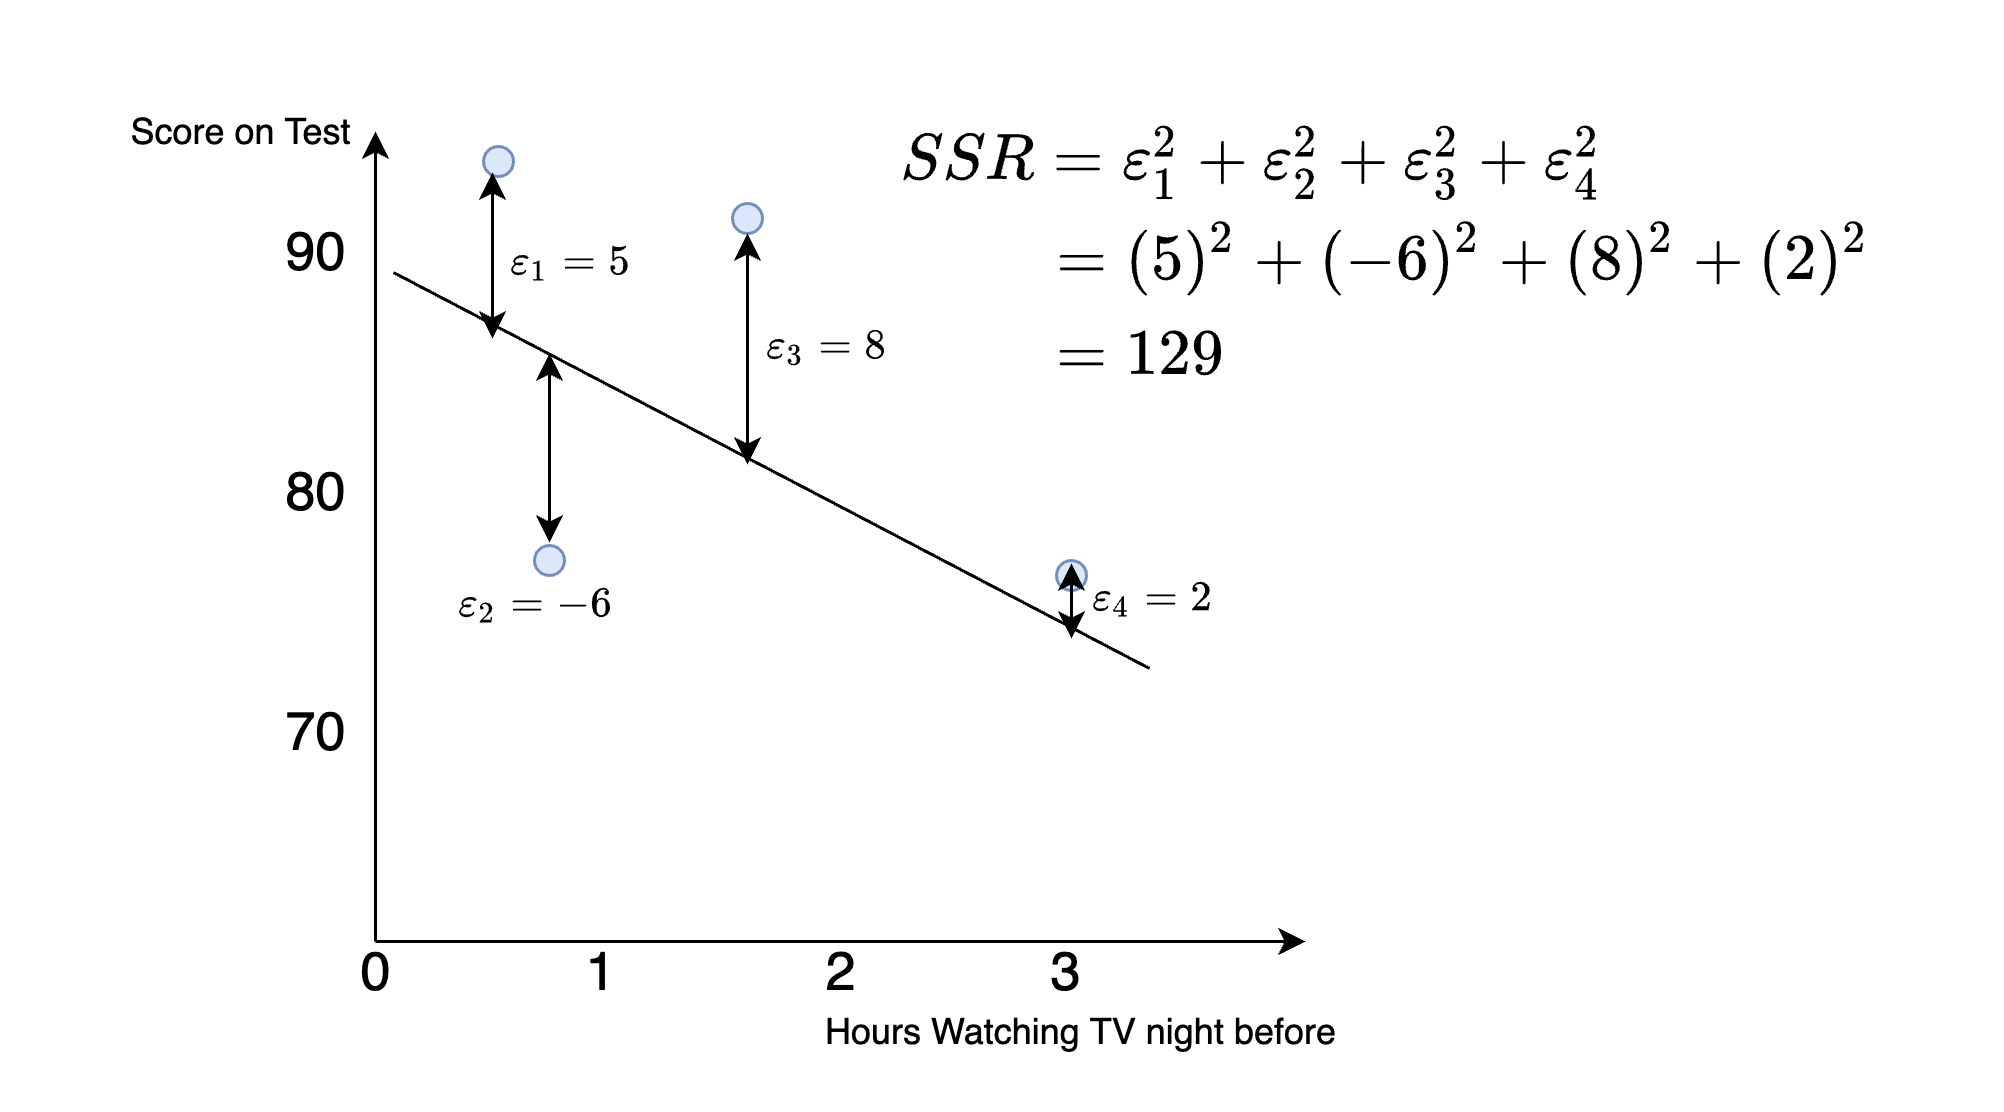
\includegraphics[width=0.9\linewidth]{images/04_reg3} 

}

\caption{Hypothetical Dataset: Finding the Best Fit Line}\label{fig:hypreg4}
\end{figure}

We can again compute the sum of squared residuals, which is now equal to:

\[
SSR = (5)^2+(-6)^2+(8)^2+(2)^2=129
\]
So comparing this to the previous line, we can see this fits better. The sum of squared residuals is smaller. Intuitively, this indicates the points we are trying to predict (the test scores) are closer to the line in Figure \ref{fig:hypreg4} than in Figure \ref{fig:hypreg3}.

Now, linear regression picks the line that minimizes the SSR. Lucky for us, we don't need to keep drawing hypothetical lines and computing the SSR to figure out the solution. There is a mathematical solution to this problem which you will learn about in future statistics or econometrics courses. What that means for our purposes is that computers can find the line that best fits the data very fast.

\section{Predicted Values}\label{predicted-values}

Now that we have learned how the linear regression line is estimated, let's talk about what we can do with this information. The first concept we will introduce is \textbf{predicted values} or \textbf{fitted values}. To understand this concept, we are first going to set up a real-world application.

For this application, we are interested in the relationship between life expectancy in a country and the average income in a country. We propose modeling life expectancy as a linear function of average income:

\[
\text{Life Expectancy}_i = \beta_0 + \beta_1 \cdot \text{Average Income in 1000s}_i + \varepsilon_i
\]

Figure \ref{fig:scatter1} plots the life expectancy in a country vs the average income, which is stored in \$1,000 US dollars. For example, a value of 50 indicates that the average income in that country is 50,000 U.S. dollars per year.

\begin{figure}

{\centering 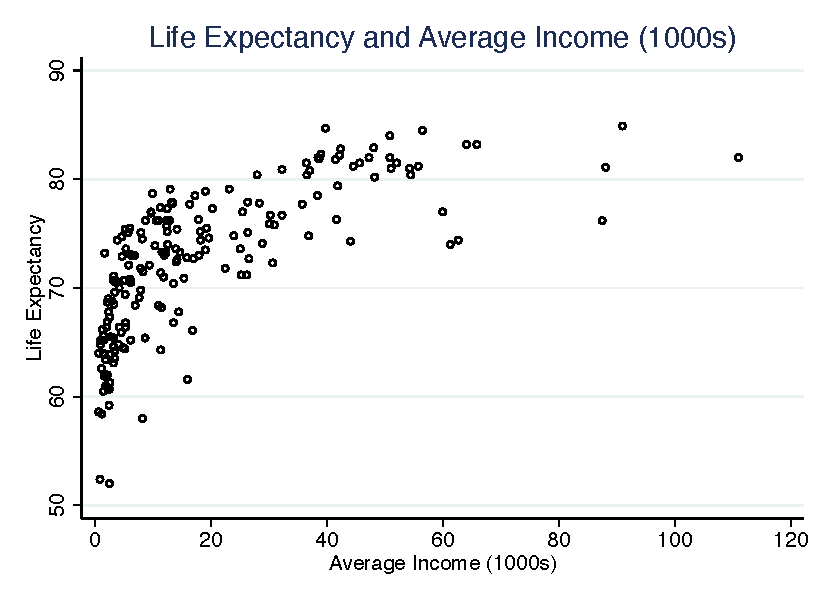
\includegraphics[width=0.9\linewidth]{images/04_scatter1} 

}

\caption{Life Expectancy vs. Average Income (1000s) Across Countries}\label{fig:scatter1}
\end{figure}

Imagine now we use linear regression to fit a line to the data in Figure \ref{fig:scatter1}. Imagine we find \(\hat{\beta_0}=67.97\) and \(\hat{\beta_1}=0.24\). These values define a line with an intercept equal to 67.97 and a slope equal to 0.24. Our question now is, what can we do with this information?

Well, one thing we can do is form predictions for life expectancy given a value of average income. In other words, if I tell you a country's average income, you could use the linear regression estimates to predict what the life expectancy in that country is. In social sciences, there is sometimes less emphasis on prediction. However, in many settings, one might be interested in forming predictions. For example, imagine you work for a company that is trying to predict who will buy their good based on the characteristics of individuals. You could use linear regression for this prediction problem. In policy settings, decisions often depend on predictions. For example, a policymaker may want to predict whether a given defendant will recidivate if released on parole. Linear regression is one (powerful) way to form predictions. It is likely the first tool you will learn in most machine learning classes which focuses primarily on prediction.

Imagine I tell you a country has an average income of \$50k. How do we use the regression results to form our best guess for the life expectancy in this country? Well, to begin, let's plot the line that best fits the data. The orange line in Figure \ref{fig:bestfit1} is the line of best fit. It is a line with an intercept equal to 67.97 and a slope coefficient equal to 0.24.

\begin{figure}

{\centering 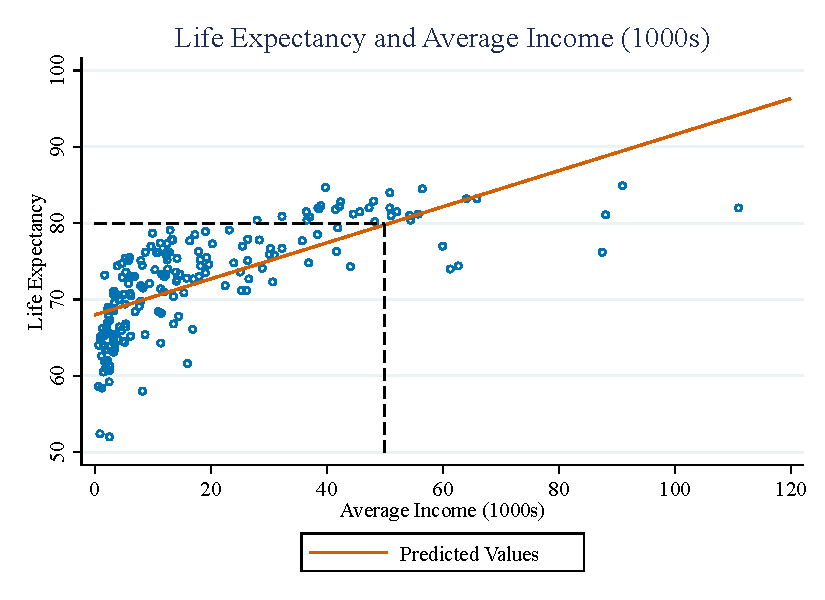
\includegraphics[width=0.9\linewidth]{images/04_scatter1p5} 

}

\caption{Life Expectancy vs. Average Income (1000s) Across Countries}\label{fig:bestfit1}
\end{figure}

One way to interpret this line is that this is our best (linear) prediction of life expectancy given average income. In other words, if we want to predict the life expectancy for a country with an average income of \$50k, we can just find what our line would predict for this country. In Figure \ref{fig:bestfit1}, we have added a dashed line at an average income \$50k. At an average income of \$50k, it appears as if the value of the line is around 80. But we don't need to just eyeball this graph to figure this information out. We have the exact parameters of this line from our regression estimates. We know the intercept is 67.97 and the slope coefficient is 0.24. Therefore, we can use the linear equation to form the predicted life expectancy of a country with income equal to \$50k:

\[
\text{Predicted Life Expectancy}_i = 67.97 + 0.24 \cdot 50 = 79.97
\]

In general, if you want to form the predicted value for an observation with a value of \(X_i\), you can form

\[
\text{Predicted Y}_i = \hat{Y}_i= \hat{\beta_0} + \hat{\beta}_1 \cdot X_i
\]
It is common to denote the predicted value for an observation \(i\) as \(\hat{Y}_i\).

Now, of course, any prediction is prone to error. Even complex predictions that use potentially hundreds of variables won't always be right. For example, Netflix uses a complicated machine-learning algorithm to predict what shows to recommend you. But they are sometimes wrong. Sometimes you are not interested in the recommended shows.

Therefore, it is often helpful to characterize the error associated with a model. For a given observation, the error associated with the model is given by

\[
\text{Error}_i = \text{Actual}_i-\text{Predicted}_i
\]

For example, the U.S.'s average income is 60k. If I use the regression model to predict Life Expectancy, I would get:

\[
\text{Predicted Life Expectancy}_i = 67.97 + 0.24 \cdot 60 = 82.37
\]

In other words, based on the U.S.'s average income, I expect the life expectancy to be 82.37 years. But when I look in the data, I see that it is actually 77 years. Therefore, the error associated with the U.S. is equal to

\[
\text{Error}_i = \text{Actual}_i-\text{Predicted}_i = 77-82.37=-5.37
\]
Therefore, the actual life expectancy in the U.S. is 5.37 years lower than the life expectancy predicted by the linear model.

As we have alluded to, there are other ways to form predictions. In certain cases, this linear model might not be an appropriate way to model the data. Maybe the relationship does not appear particularly linear. For example, in Figure \ref{fig:scatter1}, it appears at low incomes, an increase in income results in a very steep rise in life expectancy. Then, at higher incomes, near \$60k, \$70k, it doesn't appear that increases in income are associated with increases in life expectancy. If I were given free discretion to draw a \textbf{curve} to the data, the curve would start out steep at low incomes, and get flatter at high incomes. In other words, the curve would be nonlinear.

We are not going to cover nonlinear methods in this course. But it turns out that we can sometimes improve our model by simply changing the variables a bit. What we are going to try next is to estimate a linear regression that models life expectancy as a function of the \textbf{natural logarithm of average income}. In other words, we will estimate a linear regression of the following form.

\[
\text{Life Expectancy}_i = \beta_0 + \beta_1 \cdot \text{Ln(Average Income)}_i + \varepsilon_i
\]

The key difference is that we now have \textbf{Ln(Average Income)} as our explanatory variable. \textbf{Ln()} stands for natural logarithm. You have probably seen a graph with one of the variables ``logged''. This can be done for a few reasons. First, it can reduce the influence of outliers. The natural logarithm is a concave function, which in simple terms, means it shrinks large numbers more than it shrinks small numbers. A second reason that you often see logged graphs is that the relationship between two variables Y and X may be nonlinear, but the relationship between Y and ln(X) may be linear.

There are different bases for the logarithmic function. We will always use the natural logarithm. This is by far the most widely used and interpretable. If you ever hear or read ``log'' in this class, always interpret this as ``the natural logarithm''.

In Stata, if you want to take the natural logarithm of a variable, you can use either \texttt{log()} or \texttt{ln()}. For example, to create a variable that is equal to the natural logarithm of income, you could type either \texttt{gen\ log\_income\ =\ log(income)} or \texttt{gen\ log\_income\ =\ ln(income)}

Let's look at how ``logging'' changes our scatterplot. Figure \ref{fig:scatter3} plots life expectancy against the natural logarithm of average income. As you can see, the relationship appears more linear now. Taking the natural logarithm shrunk the values of income for countries with high incomes more than countries with low incomes. The result in this setting is that the relationship between life expectancy and log average income appears more linear than the relationship between life expectancy and average income.

\begin{figure}

{\centering 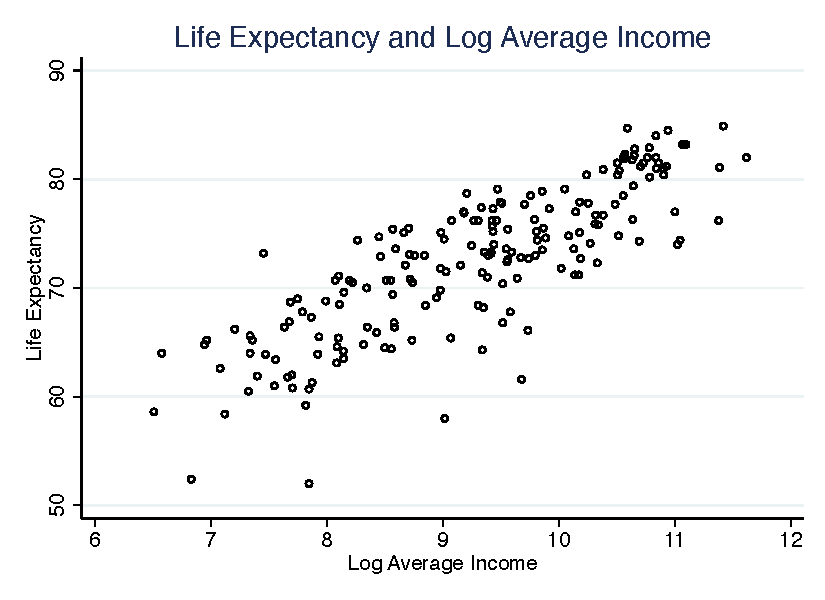
\includegraphics[width=0.9\linewidth]{images/04_scatter3} 

}

\caption{Life Expectancy vs. Log Average Income Across Countries}\label{fig:scatter3}
\end{figure}

So now imagine we find \(\hat{\beta_0}=28.69\) and \(\hat{\beta_1}=4.72\). I again ask what is the predicted life expectancy for a country with an average income of \$50k?

A very common mistake is forgetting to remember exactly what we are modeling. We are modeling life expectancy as a function of the natural logarithm of income. So to form the correct predicted value, we need to plug in \(Ln(50000)\) into the equation for our best-fit line:

\[
\text{Predicted Life Expectancy}_i = 28.69 + 4.72 \cdot Ln(50000) = 79.76
\]
Now, imagine we had forgotten to take the logarithm. If we had instead plugged in 50 (like when the X-variable was income in the thousands), we would get:

\[
\text{Predicted Life Expectancy}_i = 28.69 + 4.72 \cdot 50 =264.69
\]

We should immediately realize that 264.69 is way too high a life expectancy. You should always think about the numbers you get when forming predictions. If they seem wildly off, then you may have forgotten to transform a variable appropriately.

\section{Slope Coefficient}\label{slope-coefficient}

As social scientists, we are often interested in how changes in our explanatory variable (\(X\) variable) are associated with changes in our outcome variable (\(Y\) variable). The slope coefficient (\(\beta_1\)) in our linear regression model is informative about this.

Recall that we modeled Life Expectancy as a linear function of Average Income (1000s) and found

\[ 
\text{Predicted Life Expectancy}_i = 67.97 + 0.24 \cdot \text{Average Income 1000s}_i 
\]

The slope coefficient captures how changes in Average Income (1000s) are associated with changes in Predicted Life Expectancy.

To understand the interpretation of the slope coefficient (0.24), let's go through a simple example. Imagine I tell you I have two countries, Country A and Country B. Country A has an Average Income of \$50k. Country B has an Average Income of \$51k. What is the expected difference in Life Expectancy between these two countries?

We can form the Predicted Life Expectancy in both of these countries:
\[
\text{Predicted Life Expectancy A} = 67.97 + 0.24 \cdot 50 \nonumber \\
\text{Predicted Life Expectancy B} = 67.97 + 0.24 \cdot 51 \nonumber
\]

Taking the difference between these two yields

\[
\text{Difference in Predicted Life Expectancy} = 0.24 = \text{slope coefficient} 
\]

The slope coefficient is generally reported in order to understand the magnitude of a relationship. The general interpretation is:

Interpretation of slope coefficient: A 1-unit change in X is associated with a \textbf{slope-coefficient} unit change in the Y variable

When you actually discuss your results, though, you want to be clear about what a unit represents. For example, in our example, we would write a 1-unit change in Average Income (1000s) is associated with 0.24-year increase in Life Expectancy.

This discussion highlights an important to keep in mind when discussing results: always be clear with units. For example, in this case, our X-variable (Average Income) was denoted in the thousands. This is why 50 was plugged for the calculation of predicted life expectancy for Country A, not 50,000. To highlight the confusion that can occur if you are not careful about units, let's turn back to our regression in which X is equal to Ln(Average Income):

\[
\text{Predicted Life Expectancy}_i = 28.69 + 4.72 \cdot \text{Ln(Average Income)} 
\]
How do we interpret the slope coefficient now? A 1-unit change in Ln(Average Income) is associated with a 4.72-year increase in life expectancy.

The reason the coefficient is so much bigger now is simply because a 1-unit change in Ln(Average Income) is much larger than a 1000-dollar change in income. For example, imagine we compare two countries, one with \(\text{Ln(Average Income)}=9\) and another with \(\text{Ln(Average Income)}=10\). The Average Income in levels for a country with \(\text{Ln(Average Income)}=9\) is about 8,103 U.S. dollars (i.e.~\(Ln(8103) \approx 9\)). The Average Income in levels for a country with \(Ln(Average Income)=10\) is about \$22026 dollars. So a 1-unit change in Ln(Average Income) is quite large when translating to dollars in levels.

\textbf{Concept Check}

Try to figure out what an increase from \(Ln(Average Income)=10\) to \(Ln(Average Income)=11\) is in levels. In Stata, if you want to figure out how to transform \(Ln(Average Income)=10\) to \(Average Income\), you can type \texttt{di\ exp(10)}. This gives you the correct answer because the exponential function is the inverse of the natural logarithm function \(exp(Ln(average income))=average income\).

In almost all of our applications, we are interested in the relationship between some outcome \(Y\) and some explanatory variable \(X\). The way we gauge the magnitude of this relationship in a regression framework is through the slope coefficient. The slope coefficient captures how much we expect \(Y\) to change in response to a 1-unit change in \(X\). That is why the slope coefficient plays such a pivotal role in social science research.

\section{Regression (Stata)}\label{regression-stata}

Now that we understand the concept of linear regression, let's learn how to estimate a linear regression in Stata. To begin, we are going to set up the general linear regression framework.

\[ 
Y_i = \beta_0 + \beta_1 X_i + \varepsilon
\]

The basic syntax for the \texttt{reg} command is:

\begin{Shaded}
\begin{Highlighting}[]
\KeywordTok{reg}\NormalTok{ yvar xvar}
\end{Highlighting}
\end{Shaded}

This will produce a table with many statistics. For now we will focus on the intercept \(\hat{\beta_0}\) and slope \(\hat{\beta_1}\). To see how this works in practice, let's load up the data on life expectancy and average incomes across different countries, which is named \texttt{gapminder.dta}.

\begin{Shaded}
\begin{Highlighting}[]
\CommentTok{/*load data*/} 
\NormalTok{cd }\StringTok{"/Users/davidarnold/Dropbox/Teaching/EP5/online/04\_week/data"}
\KeywordTok{use}\NormalTok{ gapminder.dta, }\KeywordTok{replace} 
\NormalTok{file gapminder.dta }\KeywordTok{not}\NormalTok{ Stata }\KeywordTok{format}
\FunctionTok{r}\NormalTok{(610);}


\NormalTok{/Users/davidarnold/Dropbox/Teaching/EP5/online/04\_week/}\KeywordTok{data}

\NormalTok{file gapminder.dta }\KeywordTok{not}\NormalTok{ Stata }\KeywordTok{format}
\FunctionTok{r}\NormalTok{(610);}

\FunctionTok{r}\NormalTok{(610);}
\end{Highlighting}
\end{Shaded}

Reminder, we are modeling life expectancy as a function of income per capita (in the thousands). This means our dependent variable (or Y-variable) will be life expectancy and our independent variable (or X-variable) will be income per capita (in the thousands). Now let's estimate the regression:

\begin{Shaded}
\begin{Highlighting}[]
\KeywordTok{reg}\NormalTok{ life\_expectancy average\_income}
\end{Highlighting}
\end{Shaded}

\begin{verbatim}
file gapminder.dta not Stata format
r(610);


no variables defined
r(111);

r(111);
\end{verbatim}

So there are a lot of numbers in the table above. The ones we will focus on are under the column ``Coefficient.'' The first coefficient is in the row that begins with \texttt{average\_income}. This is the slope coefficient. This number tells you how a 1-unit change in \texttt{average\_income} is predicted to change the Y-variable. In this case, the regression tells us that a 1-unit change in average income (which is denoted in the 1,000s) is associated with a 0.24-year increase in life expectancy. In simpler terms, a \$1,000 dollar increase in average income is associated with a 0.24-year increase in life expectancy.

The intercept of the linear regression model appears in the next row, next to the label \texttt{\_cons}. The label \texttt{\_cons} stands for constant. The terms intercept and constant are often used interchangeably in linear regression models.

From this output, you should be able to draw the linear regression line. A good exercise is to try and draw this with pen and paper, instead of using Stata. If you can draw it correctly, then that indicates you understand the various components of this output.

It is easy to check your work using built-in functions in Stata. Stata can plot the regression line for you through the \texttt{twoway\ lfit} command. \texttt{lfit} stands for linear fit. The basic syntax of the command is to type:

\begin{Shaded}
\begin{Highlighting}[]
\KeywordTok{twoway} \KeywordTok{lfit}\NormalTok{ yvar xvar}
\end{Highlighting}
\end{Shaded}

This will plot the linear regression line from the output of:

\begin{Shaded}
\begin{Highlighting}[]
\KeywordTok{reg}\NormalTok{ yvar xvar}
\end{Highlighting}
\end{Shaded}

In our example, to plot the linear regression line, along with the scatter plot, we can type:

\begin{Shaded}
\begin{Highlighting}[]
\KeywordTok{twoway} \KeywordTok{scatter}\NormalTok{ life\_expectancy average\_income, }\CommentTok{///}
    \BaseNTok{msymbol}\NormalTok{(}\BaseNTok{circle\_hollow}\NormalTok{) msize(small) }\CommentTok{///}
\NormalTok{    || }\KeywordTok{lfit}\NormalTok{ life\_expectancy average\_income, lw(0.4) lc(}\KeywordTok{red}\NormalTok{) }\CommentTok{///}
    \BaseNTok{title}\NormalTok{(}\StringTok{"Regression of Life Expectancy on Average Income"}\NormalTok{) }\CommentTok{///}
    \BaseNTok{xtitle}\NormalTok{(}\StringTok{"Average Income (1000s)"}\NormalTok{) }\CommentTok{///}
    \BaseNTok{ytitle}\NormalTok{(}\StringTok{"Life Expectancy"}\NormalTok{) }\CommentTok{///}
\NormalTok{    graphregion(}\KeywordTok{color}\NormalTok{(}\BaseNTok{white}\NormalTok{) fcolor(}\BaseNTok{white}\NormalTok{)) }
\end{Highlighting}
\end{Shaded}

This code will generate Figure \ref{fig:bestlfit} below.

\begin{figure}

{\centering 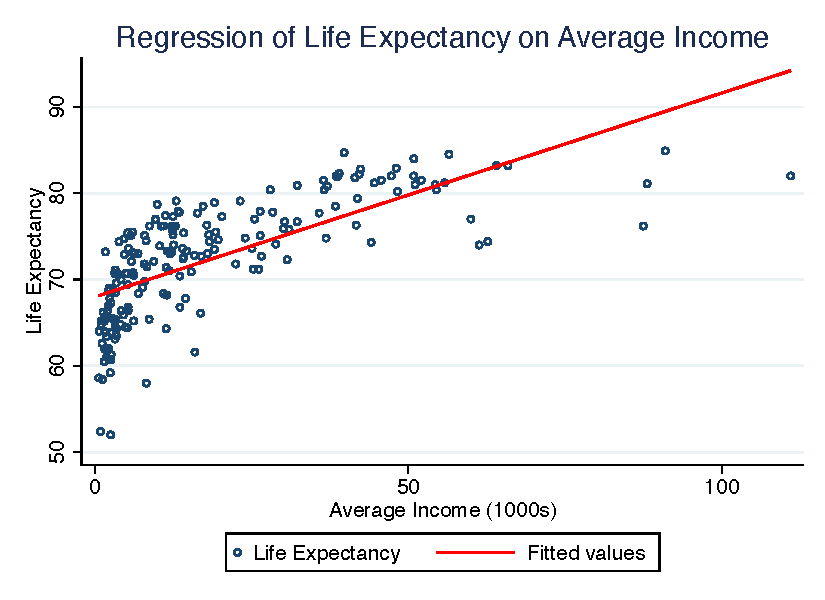
\includegraphics[width=0.8\linewidth]{images/04_best_lfit} 

}

\caption{Life Expectancy vs.Average Income Across Countries}\label{fig:bestlfit}
\end{figure}

\section{Predict}\label{predict}

In this section, we will discuss how to form predicted values in Stata. To remind you, the predicted value for an observation is equal to:

\[
\text{Predicted Value}_i = \hat{\beta_0} + \hat{\beta}_1 X_i
\]
In our example

\[ 
\text{Predicted Life Expectancy}_i = \hat{\beta_0} + \hat{\beta}_1 \cdot \text{Average Income}_i
\]
We can manually construct predicted values for every country in our dataset. We just need to take the value of average income and form predicted value using the linear regression output. However, we can also do this quickly and efficiently using the \texttt{predict} command. The most basic syntax of the \texttt{predict} command is

\begin{Shaded}
\begin{Highlighting}[]
\KeywordTok{predict}\NormalTok{ newvar}
\end{Highlighting}
\end{Shaded}

You just need to replace the word \texttt{newvar} with whatever you want the variable that holds predictions to be named.

Our first step when forming predictions is to first to estimate the regression (\texttt{predict} uses the results from the most recently executed regression estimation). In other words, the \texttt{predict} command won't work if you don't estimate a regression first. We are going to estimate the regression from the prior section:

\begin{Shaded}
\begin{Highlighting}[]
\KeywordTok{reg}\NormalTok{ life\_expectancy average\_income}
\end{Highlighting}
\end{Shaded}

\begin{verbatim}
file gapminder.dta not Stata format
r(610);


no variables defined
r(111);

r(111);
\end{verbatim}

Now that the regression has been estimated, we can form predictions

\begin{Shaded}
\begin{Highlighting}[]
\KeywordTok{predict}\NormalTok{ predicted\_life\_expectancy}
\NormalTok{file gapminder.dta }\KeywordTok{not}\NormalTok{ Stata }\KeywordTok{format}
\FunctionTok{r}\NormalTok{(610);}


\FunctionTok{last} \KeywordTok{estimates} \KeywordTok{not}\NormalTok{ found}
\FunctionTok{r}\NormalTok{(301);}

\FunctionTok{r}\NormalTok{(301);}
\end{Highlighting}
\end{Shaded}

Now a variable \texttt{predicted\_life\_expectancy} has been added to our dataset. Let's look at the value of predictions for the first three countries in our dataset.

\begin{Shaded}
\begin{Highlighting}[]
\OtherTok{list}\NormalTok{ country life\_expectancy average\_income predicted\_life\_expectancy }\KeywordTok{if} \DataTypeTok{\_n}\NormalTok{\textless{}=3}
\NormalTok{file gapminder.dta }\KeywordTok{not}\NormalTok{ Stata }\KeywordTok{format}
\FunctionTok{r}\NormalTok{(610);}


\NormalTok{no variables defined}
\FunctionTok{r}\NormalTok{(111);}

\FunctionTok{r}\NormalTok{(111);}
\end{Highlighting}
\end{Shaded}

So the first country is Afghanistan. The life expectancy in Afghanistan is equal to 63.4 years. The average income in Afghanistan is equal to 1,920 U.S. dollars per year. Given this average annual income, the linear model predicts the life expectancy in Afghanistan would be 68.4 years.

You will notice our predictions are prone to error. In some cases, we may want to generate a new variable that has the error associated with a given observation. Now that we have formed \texttt{predicted\_life\_expectancy} we can form the \texttt{error} as

\begin{Shaded}
\begin{Highlighting}[]
\KeywordTok{gen} \KeywordTok{error}\NormalTok{ = life\_expectancy {-} predicted\_life\_expectancy}
\NormalTok{file gapminder.dta }\KeywordTok{not}\NormalTok{ Stata }\KeywordTok{format}
\FunctionTok{r}\NormalTok{(610);}


\NormalTok{life\_expectancy }\KeywordTok{not}\NormalTok{ found}
\FunctionTok{r}\NormalTok{(111);}

\FunctionTok{r}\NormalTok{(111);}
\end{Highlighting}
\end{Shaded}

Let's \texttt{summarize} our new \texttt{error} variable

\begin{Shaded}
\begin{Highlighting}[]
\KeywordTok{sum} \KeywordTok{error}
\NormalTok{file gapminder.dta }\KeywordTok{not}\NormalTok{ Stata }\KeywordTok{format}
\FunctionTok{r}\NormalTok{(610);}


\NormalTok{no variables defined}
\FunctionTok{r}\NormalTok{(111);}

\FunctionTok{r}\NormalTok{(111);}
\end{Highlighting}
\end{Shaded}

The mean is about zero (which is by construction, the regression line is chosen so that on average the predictions are correct). There is a large variance though, for some countries the life expectancy is much lower than expected (negative error), while some it is much higher.

Let's look at the 3 countries with the most negative errors (implying life expectancy is much lower than predicted from income):

\begin{Shaded}
\begin{Highlighting}[]
\KeywordTok{sort} \KeywordTok{error}
\OtherTok{list}\NormalTok{ country life\_expectancy predicted\_life\_expectancy }\KeywordTok{error} \KeywordTok{if} \DataTypeTok{\_n}\NormalTok{\textless{}=3}
\NormalTok{file gapminder.dta }\KeywordTok{not}\NormalTok{ Stata }\KeywordTok{format}
\FunctionTok{r}\NormalTok{(610);}


\NormalTok{no variables defined}
\FunctionTok{r}\NormalTok{(111);}

\FunctionTok{r}\NormalTok{(111);}
\end{Highlighting}
\end{Shaded}

We can also look at the 3 countries with the most positive errors (implying life expectancy is much higher than predicted from income):

\begin{Shaded}
\begin{Highlighting}[]
\KeywordTok{sort} \KeywordTok{error}
\OtherTok{list}\NormalTok{ country life\_expectancy predicted\_life\_expectancy }\KeywordTok{error} \CommentTok{///}
\KeywordTok{if} \DataTypeTok{\_n}\NormalTok{\textgreater{}=184}
\NormalTok{file gapminder.dta }\KeywordTok{not}\NormalTok{ Stata }\KeywordTok{format}
\FunctionTok{r}\NormalTok{(610);}


\NormalTok{no variables defined}
\FunctionTok{r}\NormalTok{(111);}

\FunctionTok{r}\NormalTok{(111);}
\end{Highlighting}
\end{Shaded}

It is sometimes interesting to explore what observations are hard to predict for our model. In these countries with very negative or very positive errors, there are likely many other factors that are impacting life expectancy, besides average income. This could be why we have a hard time predicting life expectancy for these countries.

\section{Macros}\label{macros}

Before continuing our discussion of regression, we are going to discuss the concept of \textbf{macros}. Macros are simply words or characters that store certain output. In Stata, many commands store the results of commands in \textbf{macros}. For example, after the \texttt{sum} command, the value of the mean is stored in the macro \texttt{r(mean)}. To see how these work in practice, let's continue with our example that studies the relationship between life expectancy and average income.

To begin, let's summarize the \texttt{life\_expectancy} variable:

\begin{Shaded}
\begin{Highlighting}[]
\KeywordTok{sum}\NormalTok{ life\_expectancy}
\NormalTok{file gapminder.dta }\KeywordTok{not}\NormalTok{ Stata }\KeywordTok{format}
\FunctionTok{r}\NormalTok{(610);}


\NormalTok{no variables defined}
\FunctionTok{r}\NormalTok{(111);}

\FunctionTok{r}\NormalTok{(111);}
\end{Highlighting}
\end{Shaded}

The mean life expectancy is equal to 72.45. Stata has automatically stored the mean in \texttt{r(mean)}
To access the value within this macro, type:

\begin{Shaded}
\begin{Highlighting}[]
\KeywordTok{di} \OtherTok{\textasciigrave{}r(mean)\textquotesingle{}}
\NormalTok{file gapminder.dta }\KeywordTok{not}\NormalTok{ Stata }\KeywordTok{format}
\FunctionTok{r}\NormalTok{(610);}
\end{Highlighting}
\end{Shaded}

This is often useful when you want to reference a value later in your code. Copying the value from the results window can be prone to transcription errors. Using macros that store the information will lead to fewer errors.

After regressions, Stata also stores several useful results. In particular, Stata stores the value of the intercept and slope coefficient. In general, \texttt{\_b{[}varname{]}} stores the coefficient estimate for a variable named \texttt{varname}.

For example, if we estimate:

\begin{Shaded}
\begin{Highlighting}[]
\KeywordTok{reg}\NormalTok{ life\_expectancy average\_income }
\NormalTok{file gapminder.dta }\KeywordTok{not}\NormalTok{ Stata }\KeywordTok{format}
\FunctionTok{r}\NormalTok{(610);}


\NormalTok{no variables defined}
\FunctionTok{r}\NormalTok{(111);}

\FunctionTok{r}\NormalTok{(111);}
\end{Highlighting}
\end{Shaded}

Then we can retrieve the coefficient on \texttt{average\_income} by typing:

\begin{Shaded}
\begin{Highlighting}[]
\KeywordTok{di}\NormalTok{ \_b[average\_income]}
\NormalTok{file gapminder.dta }\KeywordTok{not}\NormalTok{ Stata }\KeywordTok{format}
\FunctionTok{r}\NormalTok{(610);}


\NormalTok{\_b }\KeywordTok{not}\NormalTok{ allowed when }\FunctionTok{e}\NormalTok{(b) is }\KeywordTok{not}\NormalTok{ present}
\FunctionTok{r}\NormalTok{(111);}

\FunctionTok{r}\NormalTok{(111);}
\end{Highlighting}
\end{Shaded}

You can retrieve the intercept by typing:

\begin{Shaded}
\begin{Highlighting}[]
\KeywordTok{di}\NormalTok{ \_b[}\DataTypeTok{\_cons}\NormalTok{]}
\NormalTok{file gapminder.dta }\KeywordTok{not}\NormalTok{ Stata }\KeywordTok{format}
\FunctionTok{r}\NormalTok{(610);}


\NormalTok{\_b }\KeywordTok{not}\NormalTok{ allowed when }\FunctionTok{e}\NormalTok{(b) is }\KeywordTok{not}\NormalTok{ present}
\FunctionTok{r}\NormalTok{(111);}

\FunctionTok{r}\NormalTok{(111);}
\end{Highlighting}
\end{Shaded}

Using macros can be helpful when generating new variables. For example, we can form the predicted value of each observation by forming:

\begin{Shaded}
\begin{Highlighting}[]
\KeywordTok{gen}\NormalTok{ predicted\_value = \_b[}\DataTypeTok{\_cons}\NormalTok{] + \_b[average\_income]*average\_income }
\end{Highlighting}
\end{Shaded}

We could also do this ``manually'' by copying the values of the intercept and slope coefficient from our output, but using macros ensures we will not make any transcription errors.

Not only does Stata store useful macros for you, but you can also construct your own macros in Stata. This can be useful when you are typing something over and over that is very long. Instead of repeatedly typing, you can store the information in a macro. For example, one common way to use macros is to store a list of variables. In the next example, we will create a \textbf{global macro} that stores a list of variables.

\begin{Shaded}
\begin{Highlighting}[]
\KeywordTok{global}\NormalTok{ vars = }\StringTok{"average\_income life\_expectancy"}
\NormalTok{file gapminder.dta }\KeywordTok{not}\NormalTok{ Stata }\KeywordTok{format}
\FunctionTok{r}\NormalTok{(610);}
\end{Highlighting}
\end{Shaded}

Now whenever I type \texttt{\textbackslash{}\$vars} into Stata, Stata will interpret it as ``average\_income life\_expectancy''. Let's see what happens if I type:

\begin{Shaded}
\begin{Highlighting}[]
\KeywordTok{sum} \OtherTok{$vars}
\NormalTok{file gapminder.dta }\KeywordTok{not}\NormalTok{ Stata }\KeywordTok{format}
\FunctionTok{r}\NormalTok{(610);}
\end{Highlighting}
\end{Shaded}

One could do the same thing but with a ``local'' macro.

\begin{Shaded}
\begin{Highlighting}[]
\KeywordTok{local}\NormalTok{ vars = }\StringTok{"average\_income life\_expectancy"}
\KeywordTok{sum} \OtherTok{\textasciigrave{}vars\textquotesingle{}}
\NormalTok{file gapminder.dta }\KeywordTok{not}\NormalTok{ Stata }\KeywordTok{format}
\FunctionTok{r}\NormalTok{(610);}



\NormalTok{no variables defined}
\FunctionTok{r}\NormalTok{(111);}

\FunctionTok{r}\NormalTok{(111);}
\end{Highlighting}
\end{Shaded}

So what is the difference between a local macro and a global macro. In practice, you reference a global macro with a dollar sign \texttt{\$}, a local with apostrophes `\texttt{macro\textquotesingle{}}. Both can store the same information, but locals can only be accessed within a given Stata session. Many advise to only use local macros. Setting globals can conflict with other aspects of Stata. For our purposes, we will rarely need to use macros, let alone global vs.~local. This section introduces macros as an important programming tool to understand conceptually, but it is not required to fully understand the nuances between local and global macros in Stata to understand the rest of the course material.

\section{Explore Data}\label{explore-data}

In this section, we are going to introduce the data from the experiment run by Muralidharan, Singh, and Ganimian (2019). To begin exploring the data, we are going to explore achievement gaps. The motivation for this paper is that many students in India are not at their grade level in terms of understanding. If students are not at their grade level, they may not actually learn much from attending school. In this section, we will document that (1) on average students are performing well below grade level and (2) a year in school is not associated with an additional year of understanding.

The variables we will be exploring are in the dataset \texttt{mindspark\_levels.dta}. \texttt{class} is the grade the student is enrolled in. \texttt{mathelevel} is the assessed level of the student's understanding. Therefore, if an individual's class is greater than their assessed math level, they are behind in their understanding of the curriculum.

To begin, let's provide a scatter plot of assessed math level on actual grade. Our first step will be to load the data:

\begin{Shaded}
\begin{Highlighting}[]
\NormalTok{cd }\StringTok{"/Users/davidarnold/Dropbox/Teaching/EP5/online/04\_week/data"}
\KeywordTok{use}\NormalTok{ mindspark\_levels.dta, }\KeywordTok{clear}
\NormalTok{file gapminder.dta }\KeywordTok{not}\NormalTok{ Stata }\KeywordTok{format}
\FunctionTok{r}\NormalTok{(610);}


\NormalTok{/Users/davidarnold/Dropbox/Teaching/EP5/online/04\_week/}\KeywordTok{data}
\end{Highlighting}
\end{Shaded}

The most basic scatterplot we could create from this data is displayed below

\begin{Shaded}
\begin{Highlighting}[]
\KeywordTok{set} \DecValTok{scheme}\NormalTok{ plotplainblind}
\KeywordTok{twoway} \KeywordTok{scatter}\NormalTok{ mathlevel }\KeywordTok{class}
\end{Highlighting}
\end{Shaded}

\begin{figure}

{\centering 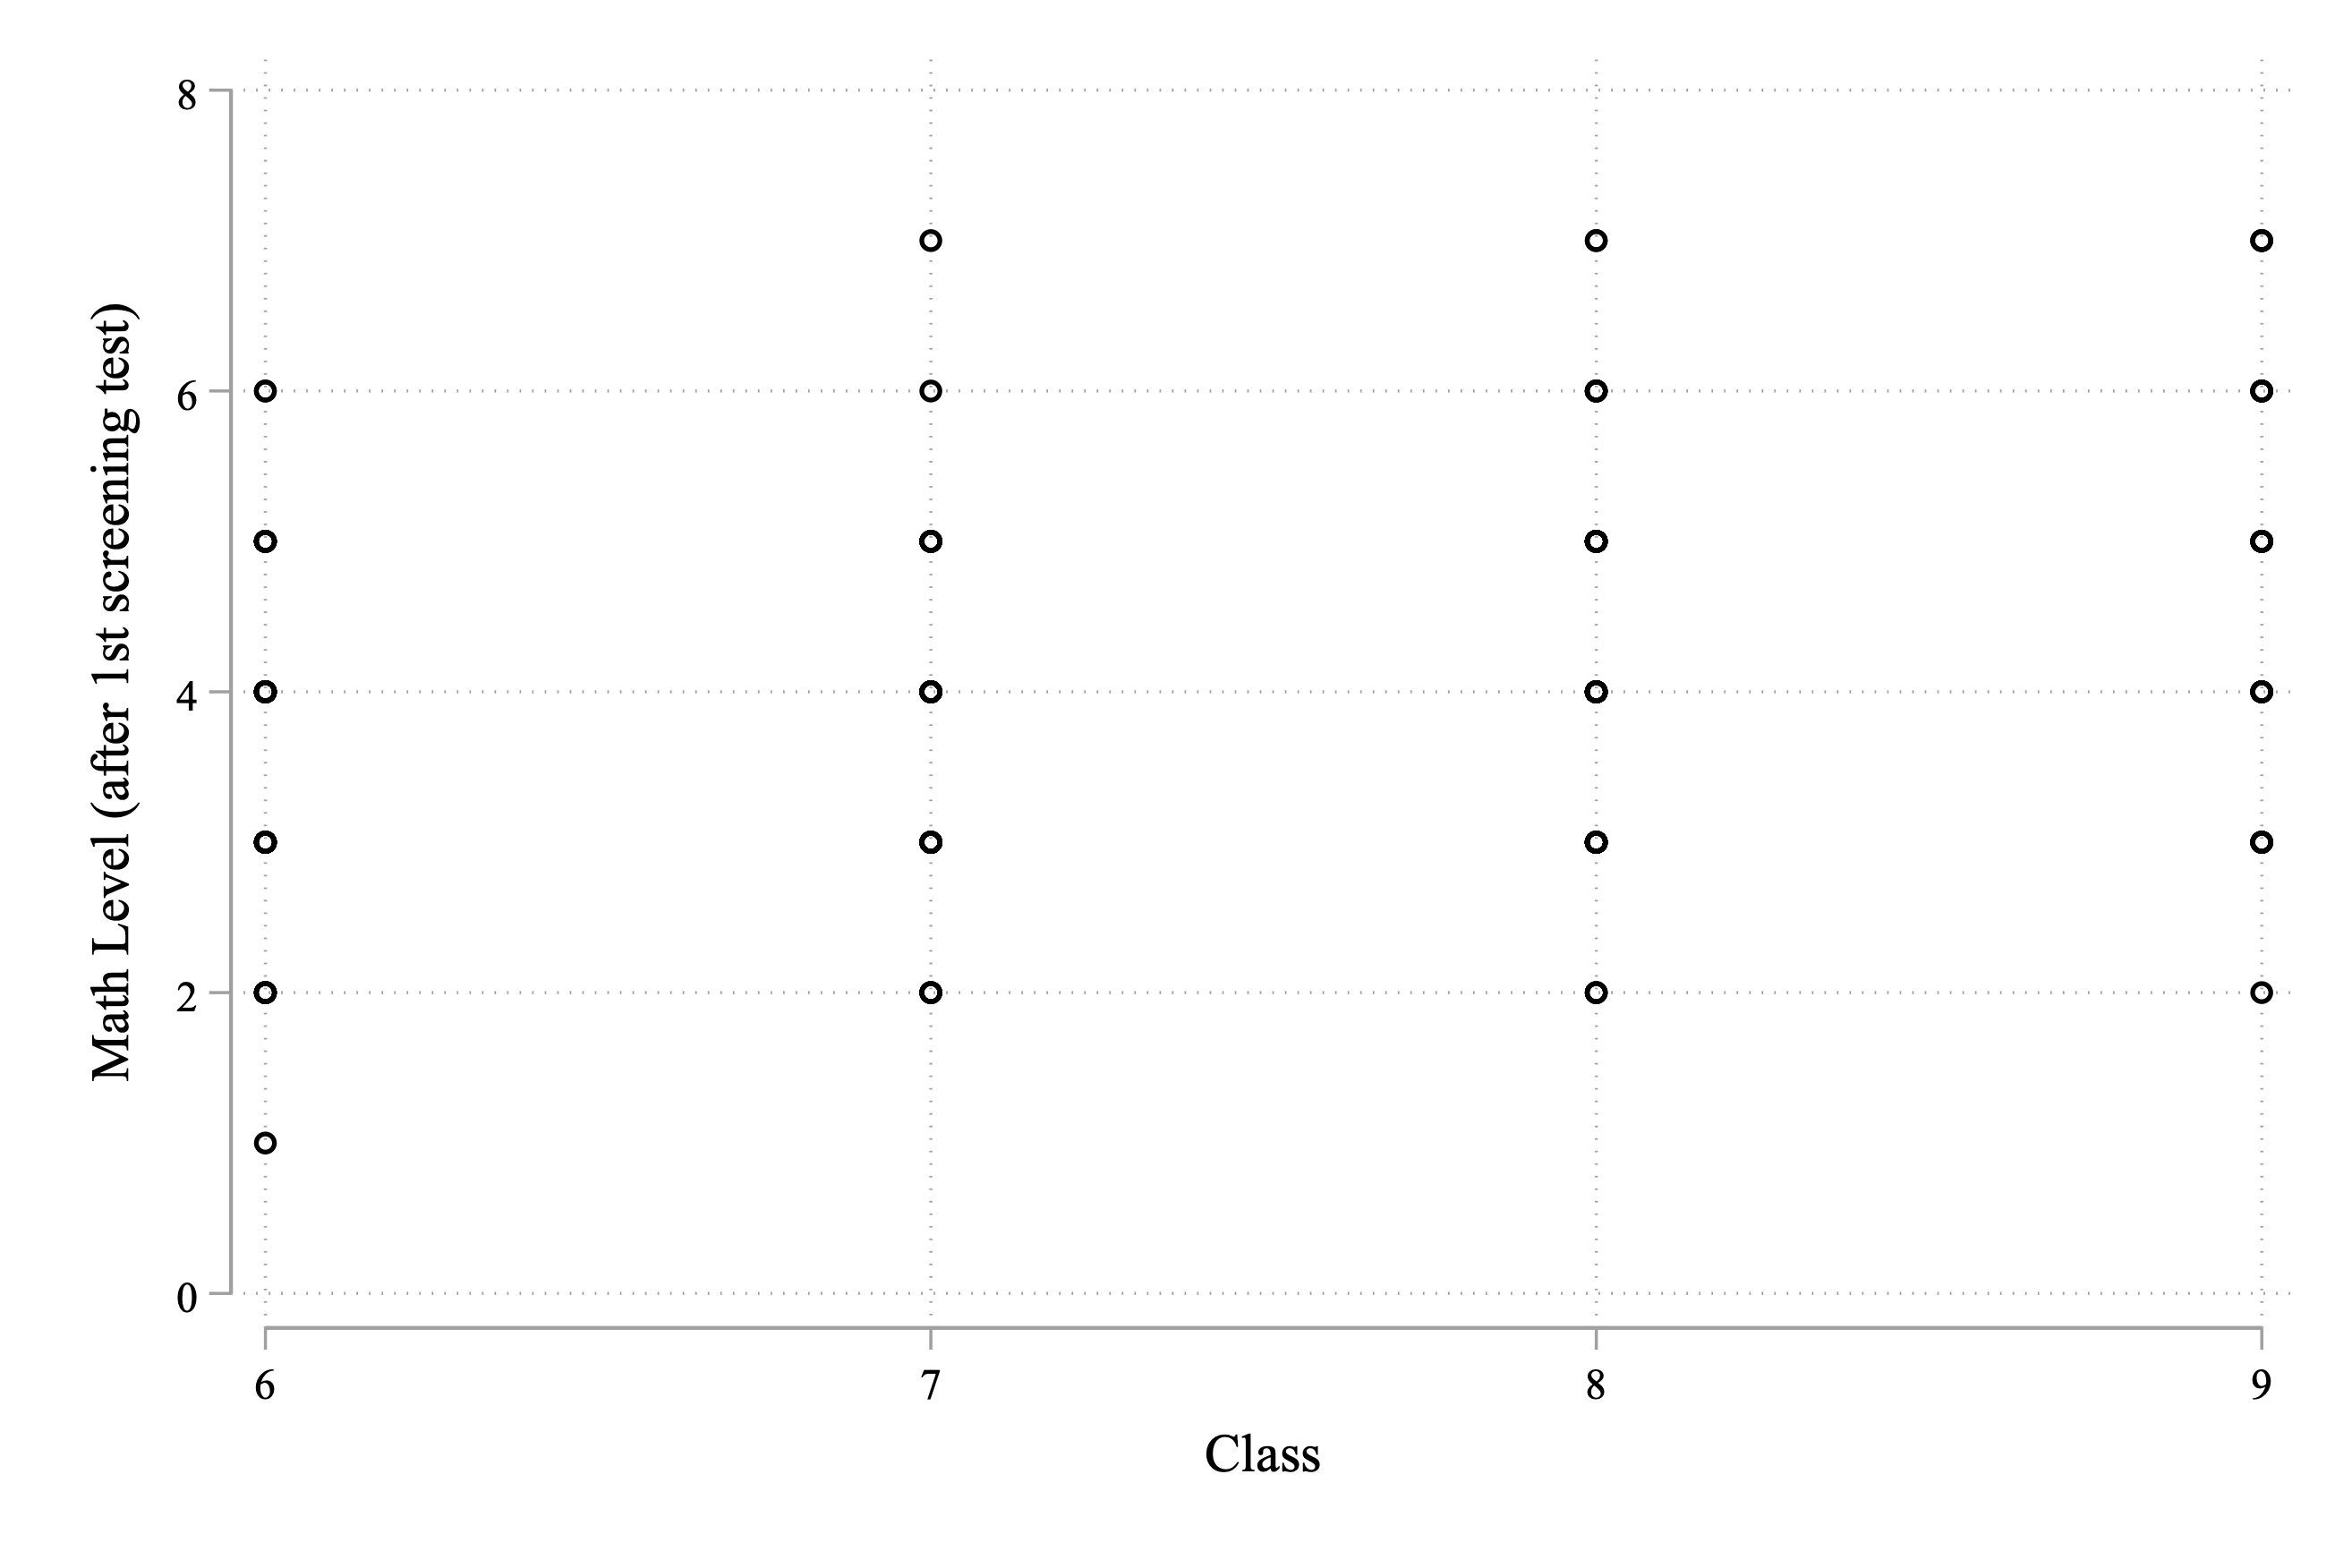
\includegraphics[width=0.8\linewidth]{images/04_basic} 

}

\caption{Assessed Math Grade Level vs. Actual Grade Level }\label{fig:basicscatter}
\end{figure}

Figure \ref{fig:basicscatter} doesn't seem particularly informative. The reason is because so many points are overlapping. We know that there are over 600 participants in the experiment, but we only see a handful of dots in the graph. The reason is that many individuals have the same values for these variables. In other words, there are many people, for example, with an assessed math level equal to 4 and an actual grade level equal to 6. From this figure, however, we can't tell how many. One way we can improve the graph is to use the \texttt{jitter()} option.

Scatter plots give us a transparent way to view our data, but when variables are categorical (like \texttt{grade} and \texttt{mathlevel} in our example), they can be less informative because so many observations overlap. \texttt{jitter()} adds a small amount of noise (small perturbations) to the data so that the points no longer overlap on the graph. The way it works is that in parentheses you place a number that determines how much noise is added. \texttt{(5)} is a common choice. A value of \texttt{(100)} would make it so that the graph is completely dominated by noise.

To understand what \texttt{jitter()} does, let's try it out on our scatter plot.

\begin{Shaded}
\begin{Highlighting}[]
\KeywordTok{twoway} \KeywordTok{scatter}\NormalTok{ mathlevel }\KeywordTok{class}\NormalTok{, jitter(5) }\CommentTok{///}
    \KeywordTok{xlabel}\NormalTok{(5(1)10) }\CommentTok{///}
    \BaseNTok{xtitle}\NormalTok{(}\StringTok{"Grade enrolled in"}\NormalTok{) }\CommentTok{///}
    \BaseNTok{ytitle}\NormalTok{(}\StringTok{"Assessed grade level of student achievement"}\NormalTok{) }
\end{Highlighting}
\end{Shaded}

\begin{figure}

{\centering 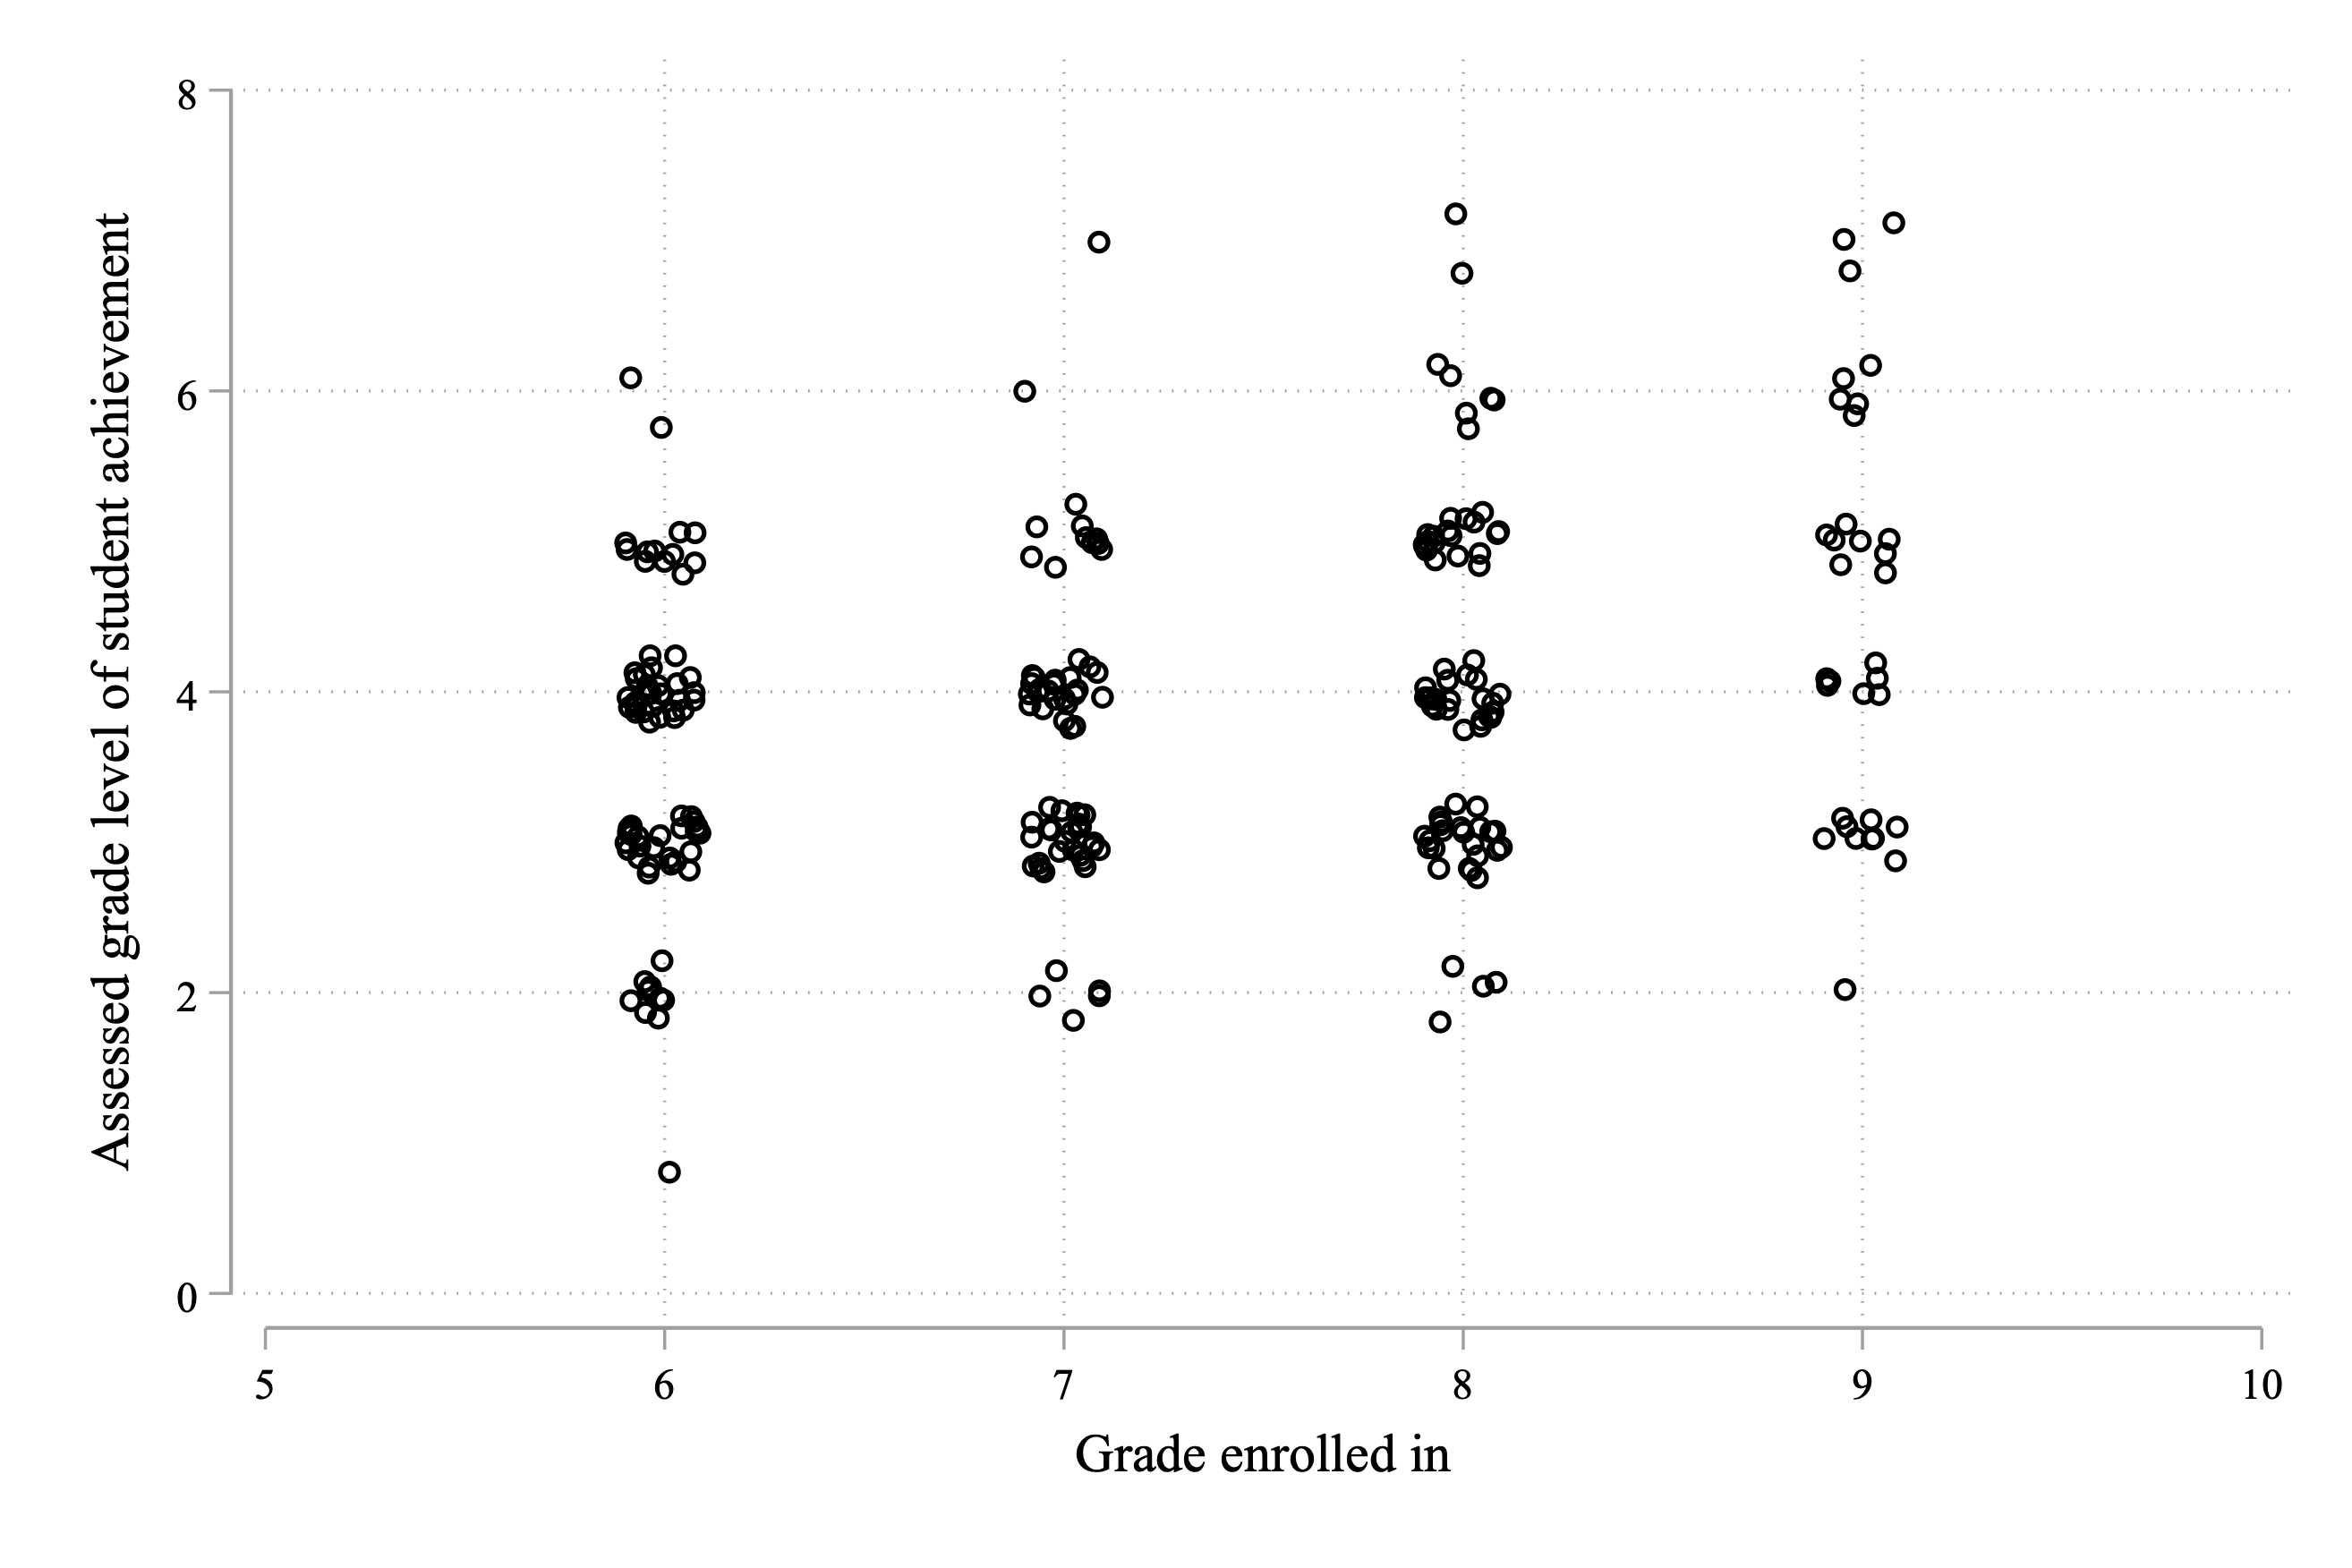
\includegraphics[width=0.8\linewidth]{images/04_improved} 

}

\caption{Assessed Math Grade Level vs. Actual Grade Level }\label{fig:improvescatter}
\end{figure}

As you can see in the figure, very few students are performing at their grade level, with none performing above grade level. There are large clusters at grades several years below grade level. For example, for students in grade 6, the largest clusters are at 4th-grade math level and 3rd-grade math level. This gives us a sense of the scope of the issue. Students' understanding is well below their grade level.

Next, let's try to get a sense of how learning is evolving over time. There are two potential ``stories'' here. Story 1: students are below grade level, but each year they are still learning (i.e.~increasing grade by 1 is associated with a 1-year increase in assessed math level). Story 2: students performing below grade level makes learning difficult (i.e.~increasing grade by 1 is associated with less than a 1-year increase in assessed math level). Figuring out which story is true is important. If story 1 is true, then even though students are behind, they are still learning more information every year. They won't fall further and further behind over time. But if story 2 is true, then there is a more serious issue in learning. Students are behind and falling further behind every year.

We can study this question in a regression framework. We are interested in the relationship between assessed math level and grade

\[ 
\text{Math Level}_i = \alpha + \beta \cdot \text{Grade}_i + \varepsilon_i
\]

\(\beta\) tells us how much we expect the assessed math level to increase for a 1-unit increase in Grade. If this is much lower than 1, then students will fall farther and farther behind each year. Let's estimate this regression in Stata:

\begin{Shaded}
\begin{Highlighting}[]
\KeywordTok{reg}\NormalTok{ mathlevel }\KeywordTok{class} 
\end{Highlighting}
\end{Shaded}

\begin{verbatim}
file gapminder.dta not Stata format
r(610);


no variables defined
r(111);

r(111);
\end{verbatim}

Reading the table above, we find \(\hat{\beta}=0.293\). This indicates that a 1-year increase in grade is associated with only a 0.293-year increase in assessed math level. In other words, students are learning over time, but at a much lower rate than is envisioned by the curriculum. Ideally, 1 year of schooling should be associated with an additional year of learning.

All of these results highlight a need for an intervention. We have documented (1) students (on average) are assessed to be performing below grade level, (2) there is large variation in assessed grade level within a given grade, and (3) learning over time is slower than intended. Maybe an intervention that ``Teaches at the Right Level'' can help alleviate some of these issues.

\section{Summary Statistics}\label{summary-statistics-1}

Before getting to the experimental data, we need to first make sure that the randomization was implemented correctly. To remind you, the experiment gave free Mindspark tuition to a random subset of students. But what if randomization failed for some reason? What if students who received Mindspark tuition already had better test scores than students who did not? Then we don't have a valid experiment. To check if we have a valid experiment, we should confirm that the treated and control students are similar based on observables. To present our results, we are going to learn a new command \texttt{outreg2}, which is useful for building publication-ready tables in Stata.

In most cases, \texttt{outreg2} is used to export regression estimates to different formats (hence the name). However, in this section, we are going to learn how to use it to create summary statistics. Summary statistics are incredibly important to present in research. If you open any social science article, there is a good chance the first table will be a table of summary statistics.

One type of summary statistic table we have already discussed is a balance table. In an experiment, we need to check that treatment and control individuals are ``balanced'' based on observable characteristics. In the Mindspark experiment, we have a few demographic characteristics we can check balance with respect to. To understand our eventual goal, Figure \ref{fig:msgtab} is the (beginning) of Table 1 from Muralidharan, Singh and Ganimian (2019). We don't need to replicate this format exactly, but hopefully, we can get something that looks professional.

\begin{figure}

{\centering 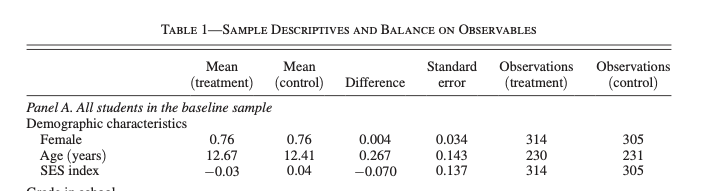
\includegraphics[width=0.8\linewidth]{images/04_msg_tab} 

}

\caption{Balance Table from Muralidharan, Singh and Ganimian (2019)}\label{fig:msgtab}
\end{figure}

The basic syntax of \texttt{outreg2} that will be appropriate for our goals is:

\begin{Shaded}
\begin{Highlighting}[]
\NormalTok{outreg2 }\KeywordTok{using} \KeywordTok{table}\NormalTok{.doc, }\FunctionTok{word} \KeywordTok{replace} \CommentTok{///}
\KeywordTok{sum}\NormalTok{(}\FunctionTok{log}\NormalTok{) eqkeep(}\KeywordTok{N} \KeywordTok{mean}\NormalTok{) }\KeywordTok{keep}\NormalTok{(}\KeywordTok{varlist}\NormalTok{)}
\end{Highlighting}
\end{Shaded}

Now, there was quite a bit of syntax in the previous code. For better or worse, commands that deal with formatting tend to have lots of options. This is good for flexibility but can make it frustrating to learn initially. Let's go through each part of the command step-by-step:

\begin{itemize}
\item
  \texttt{outreg2\ using\ table.doc} -- tells Stata that we should save the results of this command in a file called \texttt{table.doc} (it will be saved in the working directory)
\item
  \texttt{word\ replace} -- tells Stata that the format is a Word document and if it already exists in the working directory it should be replaced
\item
  \texttt{sum(log)} -- tells Stata that this should be a summary stats table. \texttt{outreg2} is usually used for regression tables, not summary statistics table
\item
  \texttt{eqkeep(N\ Mean)} -- tells Stata to keep certain statistics in the summary stats table. In this case, the observation count and the average (can also store SD, min, and max)
\item
  \texttt{keep(varlist)} -- tells Stata what variables to include. Replace \texttt{varlist} with a list of variables you want to appear in the table
\end{itemize}

Let's use the syntax above to create a summary statistics table with our data:

\begin{Shaded}
\begin{Highlighting}[]
\NormalTok{outreg2 }\KeywordTok{using}\NormalTok{ tab1\_basic.doc, }\FunctionTok{word} \KeywordTok{replace} \CommentTok{///}
\KeywordTok{sum}\NormalTok{(}\FunctionTok{log}\NormalTok{) eqkeep(}\KeywordTok{N} \KeywordTok{mean}\NormalTok{) }\KeywordTok{keep}\NormalTok{(st\_age1 st\_female1 ses\_index) }
\end{Highlighting}
\end{Shaded}

Figure \ref{fig:tab1basic} presents the basic summary statistics table. You can also customize it more before exporting by adding the option \texttt{title("Table\ 1:\ Summary\ Statistics")}. This will add a title to the table.

\begin{figure}

{\centering 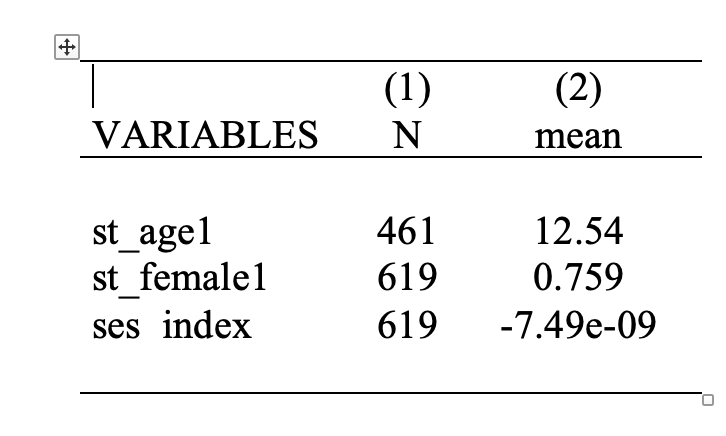
\includegraphics[width=0.8\linewidth]{images/04_tab1_basic} 

}

\caption{Basic Summary Statistics Table}\label{fig:tab1basic}
\end{figure}

Now, this isn't exactly what we wanted. We wanted a balance table, that shows the statistics of these variables by treatment status. To create this table we are going to combine \texttt{outreg2} with the \texttt{bys} command.

\begin{Shaded}
\begin{Highlighting}[]
\KeywordTok{bys}\NormalTok{ treat: outreg2 }\KeywordTok{using}\NormalTok{ balance\_tab.doc, }\FunctionTok{word} \KeywordTok{replace} \CommentTok{///}
\KeywordTok{sum}\NormalTok{(}\FunctionTok{log}\NormalTok{) eqkeep(}\KeywordTok{N} \KeywordTok{mean}\NormalTok{) }\KeywordTok{keep}\NormalTok{(st\_age1 st\_female1 ses\_index) }\CommentTok{///}
\KeywordTok{label} \CommentTok{///}
\BaseNTok{title}\NormalTok{(}\StringTok{"Table 2: Characteristics of Treatment and Control Students"}\NormalTok{)}
\end{Highlighting}
\end{Shaded}

The code above generates Figure \ref{fig:tab1balance}:

\begin{figure}

{\centering 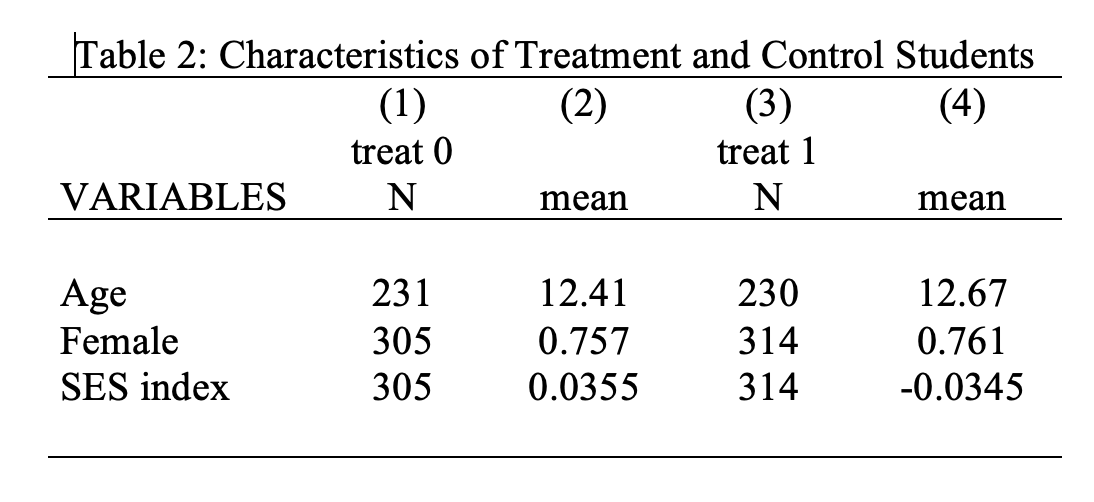
\includegraphics[width=0.8\linewidth]{images/04_balance_tab} 

}

\caption{Basic Balance Table}\label{fig:tab1balance}
\end{figure}

One limitation of our current table is that treat 0 and treat 1 is not the most descriptive way to describe the data. However, given we now have this table in Word format, we can manually make any necessary changes. For example, Figure \ref{fig:tab2balance} edits the labels to provide a table that is ready for publication.

\begin{figure}

{\centering 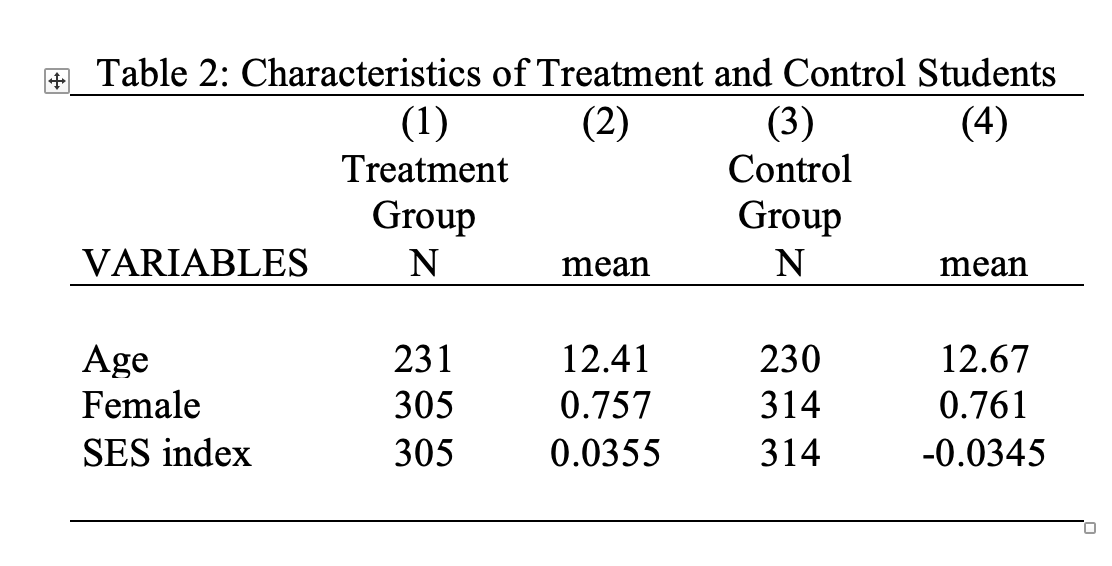
\includegraphics[width=0.8\linewidth]{images/04_balance_tab_fin} 

}

\caption{Final Balance Table}\label{fig:tab2balance}
\end{figure}

In this case, the average age, fraction female, and socioeconomic status index (ses) are all relatively similar between the treated students and control students. Looks like randomization was successful!

\section{Binary Regression}\label{binary-regression}

So far, the regression examples have been examples with continuous variables. Life expectancy and average income, for example, can take on any value within certain ranges. Therefore, these are examples of continuous variables. In this section, we are going to discuss the interpretation of regression estimates when either the dependent (Y-variable) and/or the independent (X-variable) is binary.

To start, let's consider a hypothetical example. Imagine we are interested in whether temperature impacts voting. We have an individual-level dataset that indicates whether an individual voted (\(\text{Vote}_i=1\) if voted and zero otherwise), as well as the temperature in Fahrenheit in the location they voted. We propose modeling this via a linear regression framework:

\[
\text{Vote}_i = \alpha + \beta \text{Temperature}_i + \varepsilon_i
\]

Imagine we find \(\hat{\alpha}=0.1\) and \(\hat{\beta}=0.01\). How do we interpret these numbers? Before we said the interpretation of the slope coefficient is ``the expected increase in \(Y\) for a 1-unit change in \(X\)''. If we use this interpretation, then we expect our variable \(Vote\) to increase by 0.01 if Temperature increases by a degree. A 0.01 increase in a binary indicator implies a 1 percentage point increase in the probability the value of the variable is equal to 1. This seems a little abstract, so let's consider another way to interpret this coefficient.

One way to understand this interpretation is to return to thinking about predicted values. What is the predicted value of \(Vote\) if the temperature is 50 degrees?

\[
\text{Predicted Vote} = 0.1 + 0.01*50 = 0.6
\]

Recall in earlier sections we would often take the average of binary variables. For example, in Chapter 1, we had an outcome variable that was equal to 1 if the individual passed a test and zero otherwise. We showed that the average of this variable is equal to the fraction of individuals who passed the test.

Here, what does it mean for the predicted value of vote to be equal to 0.6? It means that if the temperature is 50 degrees, we expect 60 percent of individuals to vote.

We can similarly form the predicted value of vote if it is 1 degree hotter (i.e.~51 degrees).

\[
\text{Predicted Vote} = 0.1 + 0.01*51 = 0.61
\]

Therefore, we expect 61 percent of individuals to vote if it is 51 degrees. Therefore, a 1-degree increase in temperature is associated with a 1 percentage point increase in the fraction voting. In this example, the dependent variable is binary and the independent variable is still continuous. In this next example, let's flip this, so the independent variable is continuous and the dependent variable is binary.

Let's next imagine that we are interested in the effect of a Universal Basic Income (UBI) payment on total earnings of individuals. UBI is a policy in which every individual receives a payment every month, regardless of their current income. The answer to this question has important policy implications. It might at first seem obvious that earnings will increase if an individual receives a UBI payment. But it is also possible that individuals who receive a UBI payment will respond by working less, or in extreme cases, quit working altogether. If these responses are common, it is not clear that UBI payments will actually increase the earnings of recipients overall.

There are now a few experiments on UBI that are either complete or in progress. In these experiments, some individuals receive UBI payments, while others do not. Imagine we have access to the data of one of these experiments and propose modeling earnings as a function of whether you are given access to the UBI payment (i.e.~UBI is a binary variable that is equal to 1 if the individual receives the UBI payment and zero otherwise):

\[
\text{Total Earnings}_i = \alpha + \beta \cdot \text{UBI} + \varepsilon_i
\]
Let's interpret the regression coefficients again through forming predicted values. What is the predicted earnings for someone who does not receive UBI?

\[ 
\text{Predicted Earnings} = \alpha + \beta \cdot 0 =\alpha
\]

What is the predicted earnings for someone who does receive UBI?

\[ 
\text{Predicted Earnings} = \alpha + \beta \cdot 1 =\alpha + \beta
\]
So \(\alpha\) is the predicted earnings for individuals who don't receive the UBI payment. In other words, this is the expected earnings for control workers. \(\beta\) is the difference in earnings for participants who receive UBI, relative to those who do not. In other words, if we predict control workers will have earnings of 50,000, and UBI recipients have earnings of 60,000, then \(\hat{\alpha}=50,000\) and \(\hat{\beta}=10,000\).

Finally, let's change the prior example slightly so that both the dependent and independent variables are binary. Instead of studying the impact of UBI on earnings, let's study the impact on employment:

\[
\text{Employment}_i = \alpha + \beta \cdot \text{UBI} + \varepsilon_i
\]

Now both \(Y\) and \(X\) are binary. Let's again interpret these coefficients through predicted values.

What is the predicted value of employment for someone who does not receive UBI?

\[ 
\text{Predicted Employment} = \alpha + \beta \cdot 0 =\alpha
\]
In other words, of those who do not receive UBI, we expect \(\alpha\) percent to be employed. Now, what is the predicted employment for someone who does receive UBI?

\[ 
\text{Predicted Employment} = \alpha + \beta \cdot 1 =\alpha + \beta
\]

In other words, of those who do receive UBI, \(\alpha + \beta\) percent are employed. \(\beta\) is the percentage point difference in employment rates between those who receive UBI vs.~those who do not. For example, imagine 80 percent of control workers are employed, while 75 percent of UBI recipients are employed. In this case \(\hat{\alpha}=0.80\), while \(\hat{\beta}=-0.05\). In this case, we would conclude that receiving UBI decreases the probability of being employed by 5 percentage points.

There are a few lessons from this chapter that you should internalize for the rest of this book. In order to write clearly about your results, it is important to understand if your variables are continuous or binary. If the \(Y\) variable is binary, you can interpret the \(\beta\) coefficients as changes in the probability of having \(Y=1\). For example, a 1-unit increase in temperature is associated with a \(\beta\) percentage point change in the probability of voting. If the \(X\) variable is binary indicator, then \(\alpha\) is average of \(Y\) if \(X=0\), while \(\alpha+\beta\) is average of \(Y\) if \(X=1\).

\section{Mindspark Results}\label{mindspark-results}

Now that we understand how to interpret regressions with binary variables, we are going to estimate the impact of Mindspark on test scores. To do so, we will estimate a linear regression of the following form:

\[
\text{Endline Test Score}_i = \alpha + \beta \cdot \text{Treat}_i + \varepsilon_i
\]
Endline test score ranges from 0 to 1 and represents the percent of questions that an individual got correct on the test. Treat is a binary indicator variable that is equal to 1 if the individual is in the treatment group (i.e.~was given free Mindspark tuition) and zero of the individual is in the control group (i.e.~not given free Mindspark tuition).

To begin, let's load in the dataset \texttt{mindspark\_data.dta}

\begin{Shaded}
\begin{Highlighting}[]
\NormalTok{cd }\StringTok{"\textasciitilde{}/Dropbox/Teaching/EP5/online/04\_week/data"}
\KeywordTok{use}\NormalTok{ mindspark\_data.dta, }\KeywordTok{clear} 
\NormalTok{file gapminder.dta }\KeywordTok{not}\NormalTok{ Stata }\KeywordTok{format}
\FunctionTok{r}\NormalTok{(610);}


\NormalTok{/Users/davidarnold/Dropbox/Teaching/EP5/online/04\_week/}\KeywordTok{data}
\end{Highlighting}
\end{Shaded}

Now, let's see if treatment impacts endline math scores. The endline math scores. Remember, the variable \texttt{per\_math2} contains the endline math test scores. Therefore, to estimate the impact of the treatment on this variable, we can type:

\begin{Shaded}
\begin{Highlighting}[]
\KeywordTok{reg}\NormalTok{ per\_math2 treat}
\end{Highlighting}
\end{Shaded}

\begin{verbatim}
file gapminder.dta not Stata format
r(610);


no variables defined
r(111);

r(111);
\end{verbatim}

We found that the slope coefficient \(\hat{\beta}=0.078\). Remember, our general formula for interpreting slope coefficients is a 1-unit change in \texttt{treat} is expected to increase \texttt{per\_math2} by 0.078. However, when we actually report the results, we should make it clear what these units represent. We don't want a reader to have to understand that \texttt{per\_math2} is the variable that contains the fraction correct on the math score in order to understand the interpretation. Therefore, in plain (interpretable) English, we find that students who were offered free Mindspark tuition saw a 7.8 percentage point increase in math scores relative to control students who were not offered Mindspark tuition.

\textbf{Concept Check}

What is the average score for control individuals given the regression output? What is the average score for treated individuals given the regression output? To check your answer you can type \texttt{sum\ per\_math2\ if\ treat==0} and \texttt{sum\ per\_math2\ if\ treat==1}

So overall, Mindspark has a reasonably large impact on test scores. Test scores were quite low to begin with, so a 7.8 percentage point increase is a sizeable gain in learning. Next, let's see how effective Mindspark was for Hindi:

\begin{Shaded}
\begin{Highlighting}[]
\KeywordTok{reg}\NormalTok{ per\_hindi2 treat}
\end{Highlighting}
\end{Shaded}

\begin{verbatim}
file gapminder.dta not Stata format
r(610);


no variables defined
r(111);

r(111);
\end{verbatim}

This regression tells us that treated students who were offered free Mindspark tuition saw a 6.5 percentage point increase in Hindi test scores relative to control students. Overall, this program seems very effective in increasing both math and Hindi scores.

\section{Regression Tables}\label{regression-tables}

In this section, we are going to learn how to take those results in the prior section and translate them to publication-ready tables. To accomplish this, we are again going to use the \texttt{outreg2} command. To remind you, if you have not installed this command, you need to first type \texttt{ssc\ install\ outreg2} into the command window before using the command.

Our goal is to present the two regressions below in a nice, neatly formatted table:

\begin{Shaded}
\begin{Highlighting}[]
\KeywordTok{reg}\NormalTok{ per\_math2 treat }
\KeywordTok{reg}\NormalTok{ per\_hindi2 treat}
\end{Highlighting}
\end{Shaded}

To present multiple regressions in a single table, we will take advantage of the \texttt{est\ store} command. \texttt{est\ store} stands for estimates store. It allows you to save the results of your regressions. To show how to use the command, let's estimate the impact of treatment on math scores:

\begin{Shaded}
\begin{Highlighting}[]
\KeywordTok{reg}\NormalTok{ per\_math2 treat}
\NormalTok{file gapminder.dta }\KeywordTok{not}\NormalTok{ Stata }\KeywordTok{format}
\FunctionTok{r}\NormalTok{(610);}


\NormalTok{no variables defined}
\FunctionTok{r}\NormalTok{(111);}

\FunctionTok{r}\NormalTok{(111);}
\end{Highlighting}
\end{Shaded}

Now if I want to save these estimates I can type

\begin{Shaded}
\begin{Highlighting}[]
\KeywordTok{est} \KeywordTok{store}\NormalTok{ reg\_math}
\end{Highlighting}
\end{Shaded}

The part of the code that reads \texttt{reg\_math}gives the estimates a name that you will use later. You can change this name depending on your application. For example, I could have replaced \texttt{reg\_math} with \texttt{reg\_math\_scores} in the code above and the code would have executed without error. Next, let's estimate the impact of treatment on Hindi scores and store the estimates as \texttt{reg\_hindi}. To save, space, I will suppress the output of the regression:

\begin{Shaded}
\begin{Highlighting}[]
\KeywordTok{reg}\NormalTok{ per\_hindi2 treat}
\KeywordTok{est} \KeywordTok{store}\NormalTok{ reg\_hindi}
\end{Highlighting}
\end{Shaded}

Now that we have our regression estimates stored, we can construct the regression table using the \texttt{outreg2} command:

\begin{Shaded}
\begin{Highlighting}[]
\NormalTok{outreg2 [reg\_math reg\_hindi] }\KeywordTok{using}\NormalTok{ reg\_table.doc, }\FunctionTok{word} \KeywordTok{replace}
\end{Highlighting}
\end{Shaded}

Let's go through each step of the code

\begin{itemize}
\item
  \texttt{outreg2\ {[}reg\_math\ reg\_hindi{]}} -- tells Stata to use \texttt{outreg2} to create a regression table. The table will have two columns: one that displays the math regression results and one that displays the Hindi results.
\item
  \texttt{using\ reg\_table.doc} -- tells Stata to create a new file named \texttt{reg\_table.doc} in the working directory that contains the regression table.
\item
  \texttt{,\ word\ replace} -- tells Stata the table should be in Word format, and if a file named \texttt{reg\_table.doc} already exists, then replace it with the new table.
\end{itemize}

Now let's see what this command generates.

\begin{figure}

{\centering 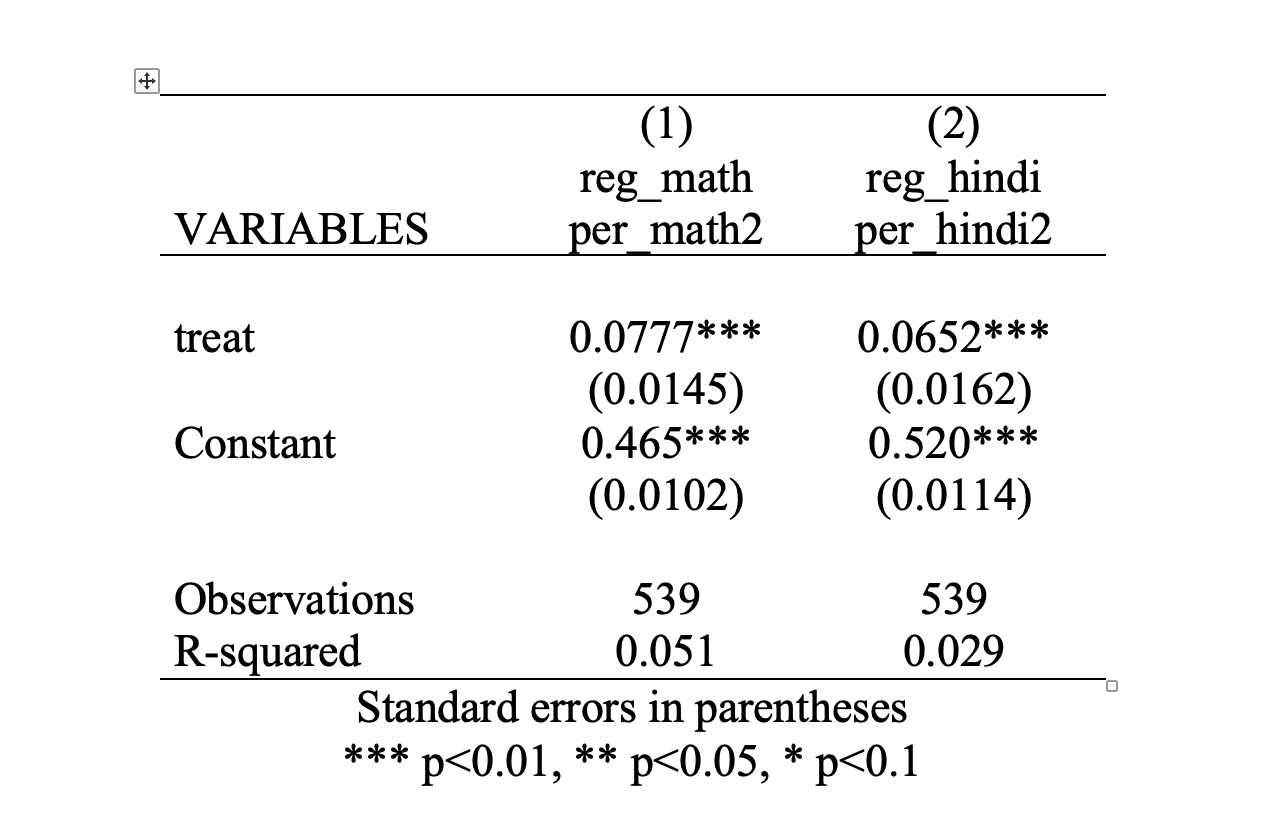
\includegraphics[width=0.8\linewidth]{images/04_reg_table_basic} 

}

\caption{Regression Table}\label{fig:regtabbasic}
\end{figure}

There are certainly some aesthetic changes that are needed in this table. But before we get to these, let's discuss the actual elements of the table. Many regression tables in academic articles have a similar format as the one seen here.

First, we should clarify that the numbers in each column correspond to a given regression estimate. Column 1 estimates the impact of Mindspark on math test scores, while column 2 estimates the impact of Mindspark on Hindi test scores. Generally, the column is titled with the dependent variable. Therefore, in this case, we can see that the dependent variable in column 1 is \texttt{per\_math2} and the dependent variable in column 2 is \texttt{per\_hindi2}.

Then, in each row, we have independent variables. In this case, our regressions have the same independent variable: \texttt{treat}. In addition to any independent variables, regression estimates (generally) display the constant (also known as the intercept) as well.

The coefficient estimates are then given by the numbers that are not in parentheses. See Figure \ref{fig:regcoefs}, which highlights the coefficient estimates in the table. If you are confused about what the numbers correspond to, you should go back to your original regression output in Stata, and see how the estimates from those regressions map to this table.

\begin{figure}

{\centering 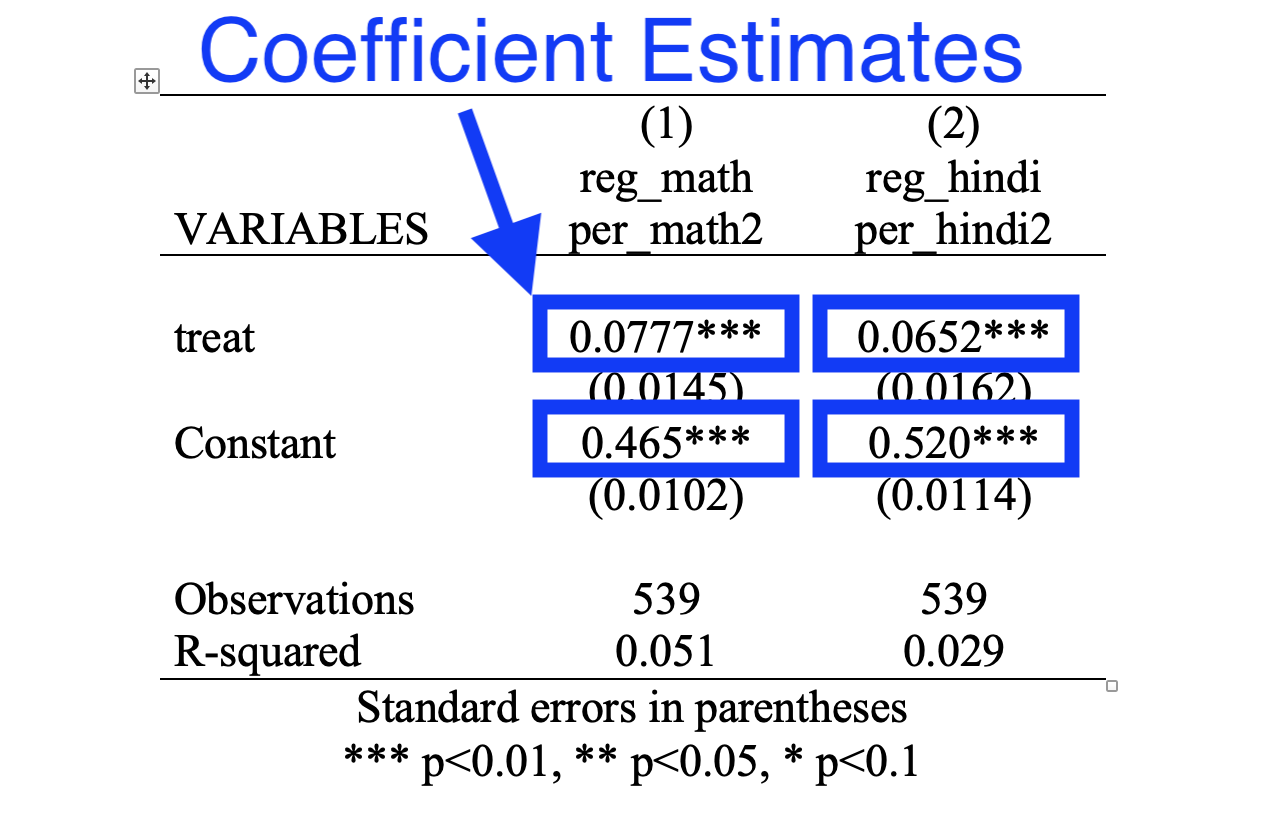
\includegraphics[width=0.8\linewidth]{images/04_reg_table_coefs} 

}

\caption{Regression Table: Coefficient Estimates}\label{fig:regcoefs}
\end{figure}

Now, there are a lot of elements in this table that we haven't explained yet. Standard errors (in parentheses) and p-values (indicated by the stars) are concepts we will not discuss in this course. In research, generally, it is important to not understand the magnitude of a treatment effect, but also whether it is statistically significant. We have not defined the concept of statistical significance. You will learn about this in other statistics or econometrics courses. Both standard errors and p-values (indicated by the stars) are related to the statistical significance of the results.

Finally, the R-squared is a measure of how much variation we can explain using our explanatory variables. The concept of R-squared is something you will learn in future statistics or econometrics courses as well and will not be a subject we cover in this course.

Now that we understand the format of the table, let's edit the table in order to make it more easily interpretable for a reader. First, we should add a descriptive title. You can do this by using the \texttt{title()} option of \texttt{outreg2}. Second, we can delete a few superfluous items, such as ``VARIABLES'', ``reg\_math'' and ``reg\_hindi''. You can do this by directly editing the table in Word. Lastly, it is better to use full phrases that describe your variables, not the variable names we have in the code. Again you can make these edits in Word. After making these changes, we finally have a nice, publication-ready regression table:

\begin{figure}

{\centering 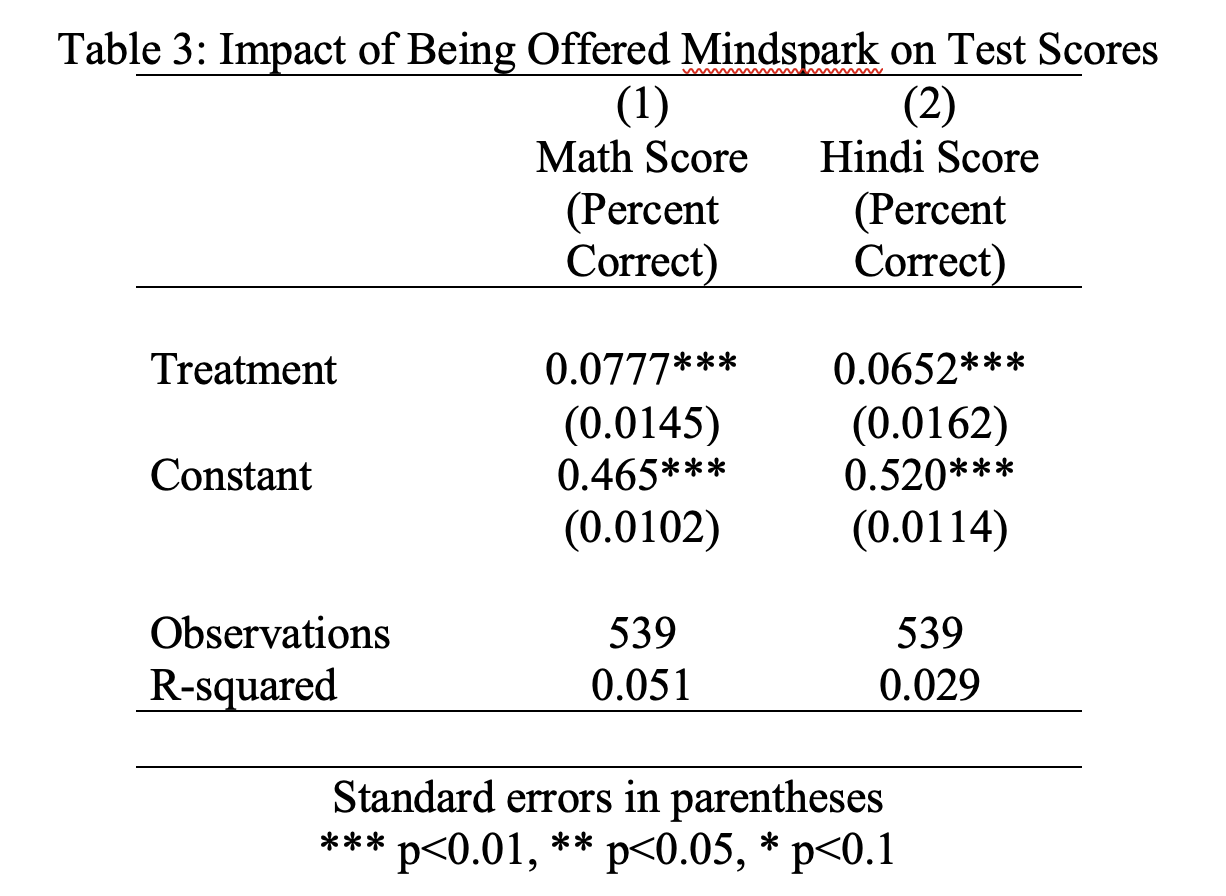
\includegraphics[width=0.8\linewidth]{images/04_reg_table_improved} 

}

\caption{Final Regression Table}\label{fig:regfinal}
\end{figure}

\section{Conditional Regressions}\label{conditional-regressions}

So far we have found that Mindspark is effective in increasing test scores in both math and Hindi on average. But maybe it is more effective for some students relative to others. In this section, we are going to explore treatment effect heterogeneity. Often it is important to understand treatment effect heterogeneity if you are trying to understand how this treatment will work in other settings. For example, would we find different results if this were implemented in an all-girls or all-boys school? Would we find different results if this were implemented in wealthier neighborhoods? Would it be a less useful treatment in areas in which achievement was already high to begin with? We can use our existing experiment to see if the treatment effect varies by different characteristics, such as gender, socioeconomic status, and baseline achievement.

So how do we estimate treatment effect heterogeneity? Well, if we want to estimate the treatment effect for females only, for example, then we should restrict our sample to females. Then, among this smaller sample of participants, we can estimate the treatment effect.

The easiest way to implement this idea in Stata is through the use of conditional regressions. In this case, the word conditional implies that individuals who meet some certain condition are included in the estimation.

For example, if we want to estimate the treatment effect in a linear regression framework, but restricted only to females, we can type:

\begin{Shaded}
\begin{Highlighting}[]
\KeywordTok{reg}\NormalTok{ per\_math2 treat }\KeywordTok{if}\NormalTok{ st\_female1==1}
\end{Highlighting}
\end{Shaded}

\begin{verbatim}
file gapminder.dta not Stata format
r(610);


st_female1 not found
r(111);

r(111);
\end{verbatim}

The part of the code \texttt{st\_female1==1} implies the regression \texttt{reg\ per\_math2\ treat} should only be estimated for females. As a result, in the regression table, you can see the Number of obs is equal to 414. These are the number of females in the experiment that have endline test scores. For comparision, let's estimate the treatment effect, but restricted only to males:

\begin{Shaded}
\begin{Highlighting}[]
\KeywordTok{reg}\NormalTok{ per\_math2 treat }\KeywordTok{if}\NormalTok{ st\_female1==0}
\end{Highlighting}
\end{Shaded}

\begin{verbatim}
file gapminder.dta not Stata format
r(610);


st_female1 not found
r(111);

r(111);
\end{verbatim}

Now, in our first regression, we find \(\hat{\beta}^{female}\) = 0.071. This implies treatment increases the percent correct by 7.1 percentage points for females. In our second regression, we find \(\hat{\beta}^{male}\) = 0.102. Treatment increases the percent correct by 10.2 percentage points for males. Therefore, overall, the treatment effect is slightly larger for males relative to females. However, in both cases, it appears that overall, the treatment is quite effective.

Next, let's consider if the treatment effects vary by socioeconomic status. In the data, we have a variable named \texttt{ses\_index}. An \textbf{index} is a variable that aggregates information from many different variables. For example, in our setting, SES index captures different aspects of household wealth. It is constructed from variables that capture ownership of various consumer goods and services. A higher SES index indicates higher wealth. Our SES index is scaled so that it is on average equal to zero in our sample. Therefore, individuals with positive values of SES index are wealthier than the average student in the experiment, and individuals with negative values of SES index are poorer than the average student in the experiment. Let's test whether the treatment effect is different for students with above-average socioeconomic status vs.~below-average socioeconomic status.

Our first regression will be estimated on individuals with below-average SES index.

\begin{Shaded}
\begin{Highlighting}[]
\KeywordTok{reg}\NormalTok{ per\_math2 treat }\KeywordTok{if}\NormalTok{ ses\_index\textless{}0}
\end{Highlighting}
\end{Shaded}

\begin{verbatim}
file gapminder.dta not Stata format
r(610);


ses_index not found
r(111);

r(111);
\end{verbatim}

Our second regression will be estimated on individuals with above-average SES index.

\begin{Shaded}
\begin{Highlighting}[]
\KeywordTok{reg}\NormalTok{ per\_math2 treat }\KeywordTok{if}\NormalTok{ ses\_index\textgreater{}0}
\end{Highlighting}
\end{Shaded}

\begin{verbatim}
file gapminder.dta not Stata format
r(610);


ses_index not found
r(111);

r(111);
\end{verbatim}

In regression 1, we find \(\hat{\beta}^{lowSES}\) = 0.087. Treatment increases the percent correct by 8.7 percentage points for individuals with below-average SES. In regression 2, we find \(\hat{\beta}^{highSES}\) = 0.075. Treatment increases the percent correct by 7.5 percentage points for individuals with above-average SES. Therefore, the treatment effect is slightly larger for low-SES, but quite similar overall.

Finally, we will explore heterogeneity by baseline achievement. Maybe students that benefit the most are those that have been ``left behind''. There are many ways one could explore this question. We are going to see if individuals below the median level of baseline test scores (within their grade) have different treatment effects than those above the median level of test scores.

The first thing we need to do is create a new variable that indicates whether an individual student performed above the median or below the median in the initial baseline assessment, within their grade level. We will do this in two steps:

\begin{itemize}
\item
  Step 1: create a variable that stores the median test score within an individual's grade.
\item
  Step 2: create an indicator variable equal to 1 if the individual's test score is above the median test score and zero otherwise.
\end{itemize}

For Step 1: we are again going to combine \texttt{bys} with \texttt{egen}. We used these commands to compute the total number of stops by race and light condition in a previous chapter. To generate median test score within a grade, we can type:

\begin{Shaded}
\begin{Highlighting}[]
\KeywordTok{bys}\NormalTok{ st\_grade1: }\KeywordTok{egen}\NormalTok{ median\_test\_score=}\KeywordTok{median}\NormalTok{(per\_math1)}
\NormalTok{file gapminder.dta }\KeywordTok{not}\NormalTok{ Stata }\KeywordTok{format}
\FunctionTok{r}\NormalTok{(610);}


\NormalTok{no variables defined}
\FunctionTok{r}\NormalTok{(111);}

\FunctionTok{r}\NormalTok{(111);}
\end{Highlighting}
\end{Shaded}

Now let's generate a new variable that indicates whether a given student's test score is above or equal to the median test score within their grade

\begin{Shaded}
\begin{Highlighting}[]
\KeywordTok{gen}\NormalTok{ above\_median = (per\_math1 \textgreater{} median\_test\_score)}
\NormalTok{file gapminder.dta }\KeywordTok{not}\NormalTok{ Stata }\KeywordTok{format}
\FunctionTok{r}\NormalTok{(610);}


\NormalTok{per\_math1 }\KeywordTok{not}\NormalTok{ found}
\FunctionTok{r}\NormalTok{(111);}

\FunctionTok{r}\NormalTok{(111);}
\end{Highlighting}
\end{Shaded}

Now that we have our indicator variable, we can estimate two regressions: (1) a regression restricted to above-median performers and (2) a regression restricted to below-median performers.

\begin{Shaded}
\begin{Highlighting}[]
\KeywordTok{reg}\NormalTok{ per\_math2 treat }\KeywordTok{if}\NormalTok{ above\_median==1}
\end{Highlighting}
\end{Shaded}

\begin{verbatim}
file gapminder.dta not Stata format
r(610);


above_median not found
r(111);

r(111);
\end{verbatim}

\begin{Shaded}
\begin{Highlighting}[]
\KeywordTok{reg}\NormalTok{ per\_math2 treat }\KeywordTok{if}\NormalTok{ above\_median==0}
\end{Highlighting}
\end{Shaded}

\begin{verbatim}
file gapminder.dta not Stata format
r(610);


above_median not found
r(111);

r(111);
\end{verbatim}

We find that \(\hat{\beta}^{above}\) = 0.095. Treatment increases the percent correct by 9.5 percentage points for above-median scoring students. We find \(\hat{\beta}^{below}\) = 0.088. Treatment increases the percent correct by 8.8 percentage points for below-median scoring students. The treatment effect is slightly larger for above-median scoring students, but quite similar overall.

To summarize our results in this chapter, we tested for heterogeneity in treatment effects by (1) gender, (2) SES status and (3) baseline achievement. While we found some evidence of heterogeneity, impacts were large and positive for all groups. This provides evidence on the \textbf{external validity} of the treatment. If we expand this program to more students, perhaps with different baseline characteristics, we might predict that it will still be effective given its ability to raise test scores for different types of students.

\section{Conclusion}\label{conclusion-2}

In this final section, we will summarize what we have learned so far and then present additional results from Muralidharan, Singh, and Ganimian (2019). The motivation for Muralidharan, Singh, and Ganimian (2019) is that in certain settings, there may be a mismatch between students' level of understanding and the curriculum they are being taught. One potential tool that can be used to alleviate this problem is technology. In Muralidharan, Singh, and Ganimian (2019), the authors test if Mindspark, a software that aims to teach-at-the-right level is successful in increasing test scores. In this chapter, we used the data from this experiment and found large test score gains.

Whenever you find some experimental result, you might want to think carefully about what is driving the result. For example, the treatment in this setting is really a combination of a few things.

\begin{itemize}
\item
  The Mindspark software aims to teach-at-the-right level
\item
  This software is combined with instruction time from a teaching assistant
\end{itemize}

Although we did not focus on this second component, every Mindspark center includes instructional time with a teaching assistant. So maybe we don't need the ``technology'' component. Maybe we just need more instruction time?

Well, Berry and Mukherjee (2016)\citep{berry2016pricing} study the impact of private tutoring in Delhi. This is a very similar intervention, but without the software to teach-at-the-right level. Instead, teaching was focused on the current grade level of the student (not the assessed level). Berry and Mukherjee (2016) find no impact of this intervention. This suggests that the individual targeting aspect of the software was essential for the results.

The key difficulty that Mindspark software attempts to overcome is the huge heterogeneity in understanding in a classroom. As an instructor, teaching effectively when learning levels vary widely is difficult. Once Mindspark is programmed, it can do this automatically. We can look at the data and see how Mindspark updates material over time for different students.

\begin{figure}

{\centering 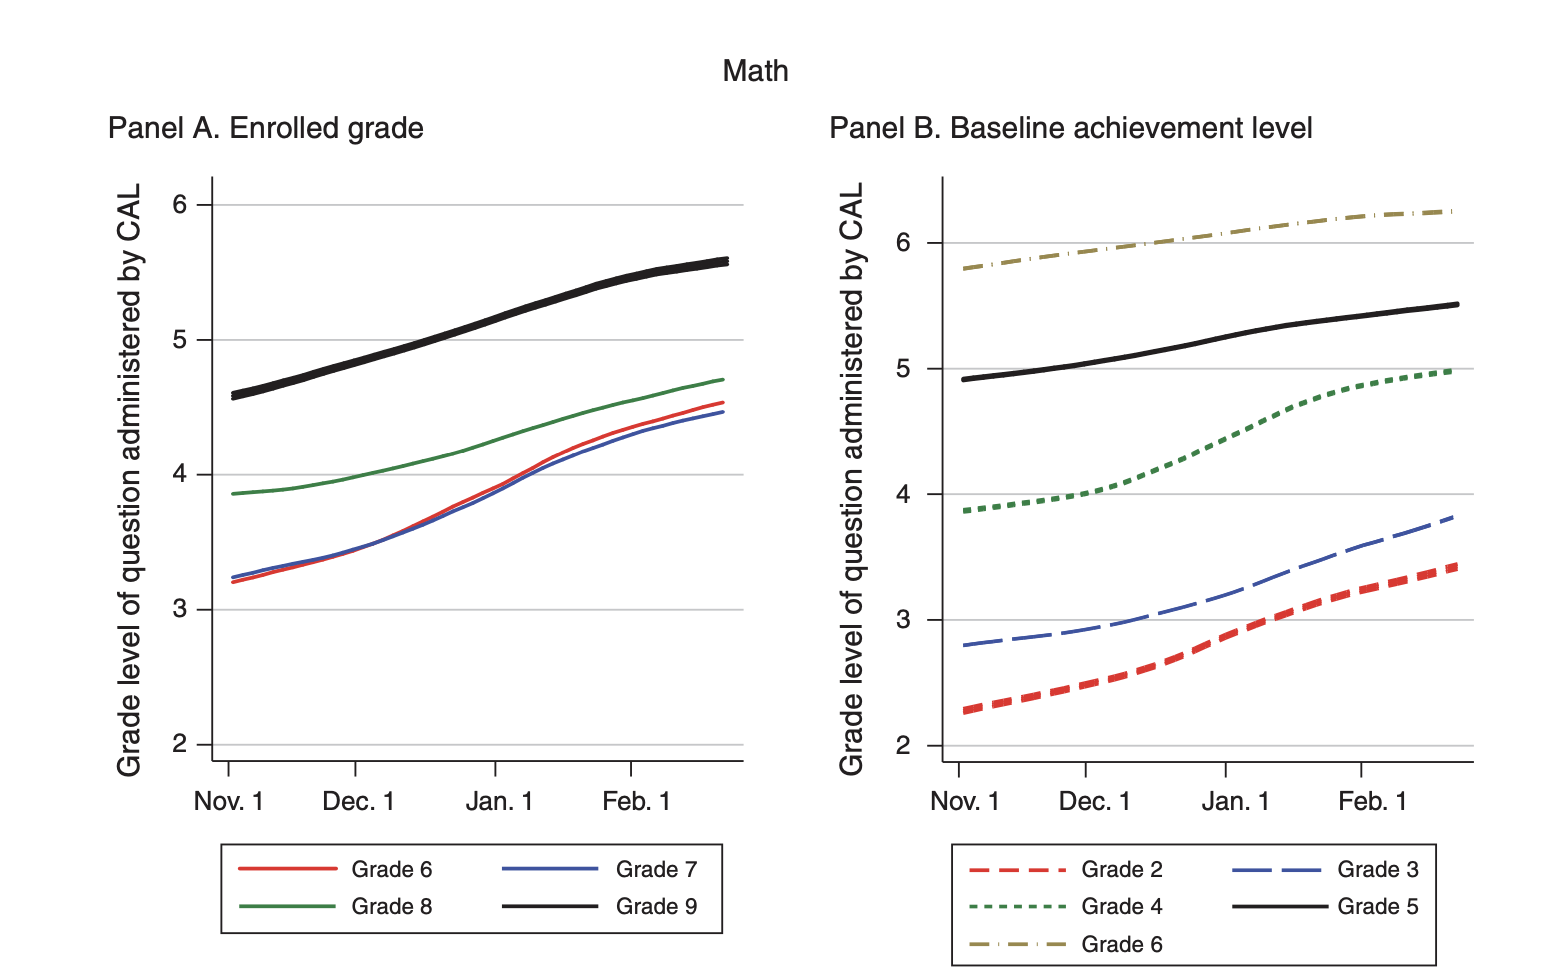
\includegraphics[width=0.8\linewidth]{images/04_fig} 

}

\caption{Dynamic Updating of Mindspark}\label{fig:dynamic}
\end{figure}

Panel A of Figure \ref{fig:dynamic} plots the grade level of questions that are proposed by Mindspark over time, for different grade levels. As you can see, individuals (on average) are starting well below grade level. For example, the solid black line is grade 9, and the questions being posed to these students are between grades 4 and 5. But over time, the assessed level increases. About 5 months later, the difficulty of the questions has increased by almost an entire year. This figure is plotting how individuals are learning over time.

Panel B, instead, plots the grade level of questions that are proposed by Mindspark over time for different levels of baseline achievement. The key takeaway from this graph is that regardless of baseline achievement, Mindspark is successful in improving updating over time. The rates of learning are quite similar for different levels of baseline achievement.

So now we are relatively certain Mindspark is successful in increasing learning, but does that imply we should invest in it as a resource for students? Whenever there is a proposed policy, there is bound to be a cost-benefit analysis. Policymakers generally have a number of different potential policies they may pursue, so you want to invest in the right policy. In order to do this, you need both the cost and benefits of the proposed policy. Running an experiment is a great way to estimate the benefits of a proposed intervention. Now that we know the benefits of Mindspark from our experiment, it is time to turn to the costs.

To do so, let's compare the cost of Mindspark to traditional government-run schools. Government-run schools spend about 240 minutes per week on Math and Hindi. The cost per pupil is around INR 1500 (US \$22). Mindspark spends about 180 minutes per week on Math and Hindi. Cost per pupil is around INR 1000 (US \$15). Using the estimates from the paper, Mindspark led to more learning in less time than government-run schools, as well as utilizing fewer financial resources.

To conclude, using technology to teach-at-the-right-level seems like a promising intervention in places in which there is tremendous heterogeneity in baseline levels of understanding. But, there is potential for even better educational design! Maybe the best intervention would blend Mindspark with standard teaching. Giving teachers more information about the level of their students could aid instruction in the classroom. This automated aspect of the software could free up teacher time for other activities that also improve student performance.

\section*{Command Descriptions}\label{command-descriptions-1}
\addcontentsline{toc}{section}{Command Descriptions}

\textbf{Commands Related to Regression}

\begin{itemize}
\item
  \texttt{reg\ yvar\ xvar} - estimates a linear regression with \texttt{yvar} being the dependent variable and \texttt{xvar} being the independent variable
\item
  \texttt{twoway\ lfit\ yvar\ xvar} - plots the linear regression line from a linea regression with \texttt{yvar} being the dependent variable and \texttt{xvar} being the independent variable
\item
  \texttt{predict\ newvar} - adds a new variable named \texttt{newvar} to the dataset that contains for each observation, the predicted value \(\hat{Y}_i = \hat{\beta}_0 + \hat{\beta} \cdot X_i\) for that observation based on the most recent linear regression estimated. This command must come after estimating a linear regression.
\item
  \texttt{reg\ yvar\ xvar\ if\ variable\ ==\ 1} - estimates a linear regression restricted only to observations for which the value of \texttt{variable} is equal to 1. This conditional statement can take on many forms. For example, if \texttt{age} is a variable in the dataset, then \texttt{reg\ yvar\ xvar\ if\ age\textgreater{}=40} will estimate a regression restricted only to observations for which the individual is older than or equal to 40 years of age.
\end{itemize}

\textbf{Formatting Tables (Not Tested on) }

\begin{itemize}
\item
  \texttt{outreg2\ using\ table.doc,\ word\ replace\ sum(log)\ eqkeep(N\ mean)\ keep(varlist)} - creates a summary statistics table that displays the mean of each variable in \texttt{varlist}, as well as the number of observations
\item
  \texttt{est\ store\ regression} - stores the estimates of a regression in a macro named \texttt{regression}. You can change the word \texttt{regression} in the code to any label you like. For example, if you are storing estimates for multiple regression, you might want to type \texttt{est\ store\ reg1} for the first regression and \texttt{est\ store\ reg2} for the second.
\item
  \texttt{outreg2\ {[}reg1\ reg2{]}\ using\ reg\_table.doc,\ word\ replace} - creates a regression table with \texttt{reg1} in the first column and \texttt{reg2} in the second. \texttt{reg1} and \texttt{reg2} are the results of two separate \texttt{est\ store} commands
\end{itemize}

\section*{Animated Concepts}\label{animated-concepts}
\addcontentsline{toc}{section}{Animated Concepts}

\chapter{Legacy of Colonial Medicine}\label{legacy-of-colonial-medicine}

\section{Colonial Medicine Intro}\label{colonial-medicine-intro}

Between 1921 and 1956 French colonial governments in Africa organized medical campaigns to treat and prevent sleeping sickness. Sleeping sickness is a lethal parasitic disease transmitted by the bite of a tsetse fly, which inhabit certain areas of Africa. During the colonial era, French colonies had military-organized campaigns exclusively focused on treating sleeping sickness.

However, the treatments at the time (Atoxyl and Lomidine) both were questionable in their efficacy and
had severe side effects. Historians and anthropologists have linked sleeping sickness campaigns to mistrust in modern medicine.

In this section, we will use data from Lowes and Montero (2021) to study how colonial medical campaigns undertaken generations ago impact health behaviors today. To do so, we will use measures of exposure to medical campaigns constructed by Lowes and Montero (2021) from newly digitized military records from France.

\begin{figure}

{\centering 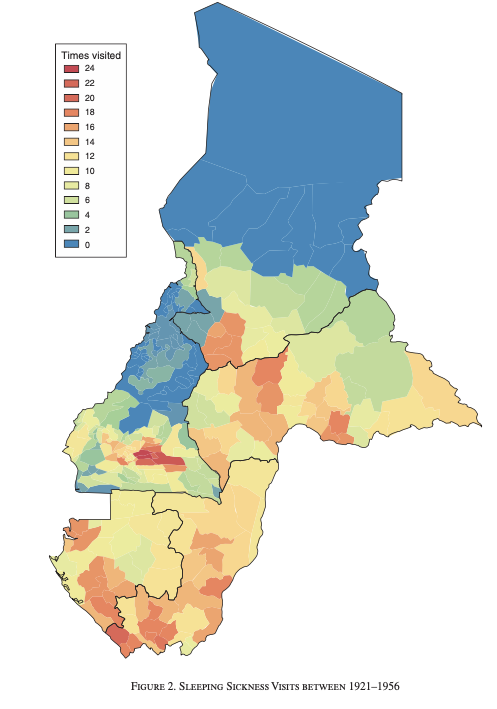
\includegraphics[width=0.45\linewidth]{images/05_map} 

}

\caption{Sleeping Sickness Visits Between 1921-1956}\label{fig:map}
\end{figure}

Figure \ref{fig:map} shows the variation in sleeping sickness across areas in Cameroon and French Equatorial Africa (present-day Central African Republic, Chad, Republic of Congo, and Gabon). As can be seen in the figure, there is large variation across areas. Some places (in blue), had no medical campaign visits related to sleeping sickness during this period. Other areas (red), were visited as many as 24 times in the years between 1921-1956. We will study how variation in these visit rates correlates to measures of trust in medicine today.

In Lowes and Montero (2021), the authors study two key outcomes, both of which come from Demographic and Health Surveys (DHS). The first is a vaccination index that captures what fraction of possible vaccines children have received. The second studies whether individuals refuse a free, non-invasive blood test. Consent to the blood test is high in these samples, as the blood test is taken by finger prick and is free to the individuals in the survey. Refusal of this blood test might then signal distrust in medicine generally.

To begin, let's load the dataset \texttt{colonial\_medicine.dta}

\begin{Shaded}
\begin{Highlighting}[]
\NormalTok{cd }\StringTok{"/Users/davidarnold/Dropbox/Teaching/EP5/online/05\_week/data"}
\KeywordTok{use}\NormalTok{ colonial\_medicine.dta, }\KeywordTok{replace}
\NormalTok{file gapminder.dta }\KeywordTok{not}\NormalTok{ Stata }\KeywordTok{format}
\FunctionTok{r}\NormalTok{(610);}


\NormalTok{/Users/davidarnold/Dropbox/Teaching/EP5/online/05\_week/}\KeywordTok{data}
\end{Highlighting}
\end{Shaded}

As usual, let's describe the data to learn more about the variables.

\begin{figure}

{\centering 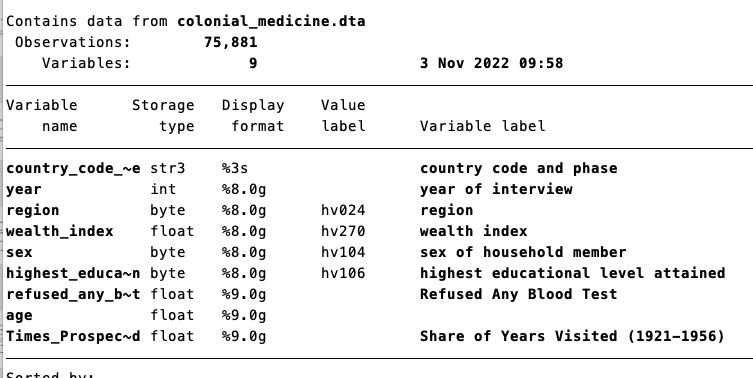
\includegraphics[width=0.75\linewidth]{images/05_describe} 

}

\caption{Describing the Colonial Medicine Data Set}\label{fig:meddescribe}
\end{figure}

So we have 75,881 survey participants, some demographics of the individual, a key outcome variable (\texttt{refused\_any\_blood\_test}), as well as a key explanatory variable (\texttt{Times\_Prospected}). To understand our key variables, let's first summarize our outcome variable.

This data is at the individual level and includes some basic demographics (age, sex, etc.) as well as our key outcome: \texttt{refused\_any\_blood\_test}

\begin{Shaded}
\begin{Highlighting}[]
\KeywordTok{sum}\NormalTok{ refused\_any\_blood\_test}
\end{Highlighting}
\end{Shaded}

\begin{verbatim}
file gapminder.dta not Stata format
r(610);


no variables defined
r(111);

r(111);
\end{verbatim}

So around 11 percent overall refuse a blood test. Our goal will be to understand if this refusal rate depends on how often an individual's area was visited during sleeping sickness campaigns in the past. The variable that captures this is \texttt{Times\_Prospected}:

\begin{Shaded}
\begin{Highlighting}[]
\KeywordTok{sum}\NormalTok{ Times\_Prospected}
\end{Highlighting}
\end{Shaded}

\begin{verbatim}
file gapminder.dta not Stata format
r(610);


no variables defined
r(111);

r(111);
\end{verbatim}

So a value of 0.2 indicates on average, an individual's location was visited 20 percent of the years between 1921-1956 (35 years total). In simpler terms, a value of 0.2 indicates 7 years, because 7 is 20 percent of 35.

So we now have the data to answer our initial question: are people who live in places in which historical medical campaigns were more prevalent more likely to refuse blood tests today? But first, let's highlight a few new aspects of the data that we will need to understand.

First, if I browse the data, you will see the variable \texttt{wealth\_index} looks like it is a string variable, yet it is highlighted in blue, not red

\begin{figure}

{\centering 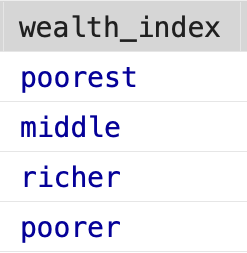
\includegraphics[width=0.25\linewidth]{images/05_values} 

}

\caption{Value Labels for Wealth Index}\label{fig:wealthlabel}
\end{figure}

If we take the average of \texttt{wealth\_index}, we do get a number out

\begin{Shaded}
\begin{Highlighting}[]
\KeywordTok{sum}\NormalTok{ wealth\_index}
\end{Highlighting}
\end{Shaded}

\begin{verbatim}
file gapminder.dta not Stata format
r(610);


no variables defined
r(111);

r(111);
\end{verbatim}

We will discuss this behavior in a future chapter about \textbf{value labels}. Next, If I browse the data, you will see the variable \texttt{refused\_any\_blood\_test} has some missing values (the period indicates the value is missing).

\begin{figure}

{\centering 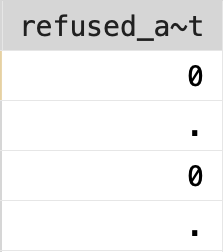
\includegraphics[width=0.25\linewidth]{images/05_missing} 

}

\caption{Missing Values}\label{fig:missingrefusal}
\end{figure}

It is important to be careful about \textbf{missing} values generally, but particularly in Stata, which we will discuss in a future chapter as well. So before we get to answering our main question, we first need to handle these data issues.

\section{Value Labels}\label{value-labels}

A value label associates a description with a particular numeric value of a variable. Sometimes it is convenient to store variables as numeric, for example, if we would like to apply some mathematical operations. However, it might be hard to remember what each value of the data represents. Value labels allow you to store the information as numeric, while still being able to quickly reference what each number represents.

In order to discuss value labels, we are going to look at the American National Election Survey. The American National Election Survey (ANES) is a survey on elections in the U.S. It has a large range of questions that come in the survey. To make it easier for users of the dataset, many of the variables have value labels attached.

We are going to load a very small subset of the dataset which has information on just a few questions:

\begin{Shaded}
\begin{Highlighting}[]
\NormalTok{cd /Users/davidarnold/Dropbox/Teaching/EP5/online/05\_week/}\KeywordTok{data}
\KeywordTok{use}\NormalTok{ anes\_subset.dta, }\KeywordTok{clear}
\end{Highlighting}
\end{Shaded}

If we browse the data, we can see some of the variables have value labels.

\begin{figure}

{\centering 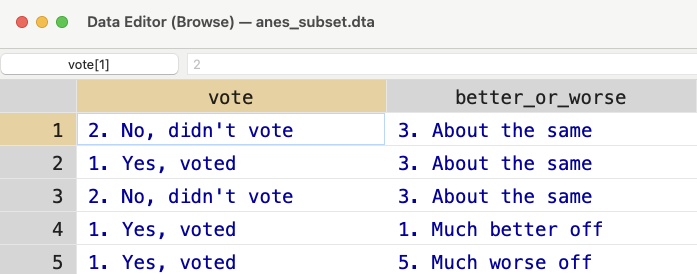
\includegraphics[width=0.75\linewidth]{images/05_br1} 

}

\caption{Browsing the ANES}\label{fig:br1value}
\end{figure}

For \texttt{vote} and \texttt{better\_or\_worse} the values look like characters, but they are highlighted in blue instead of red. What is going on? If we look closely, we can see the actual value associated with a given cell. For example, in Figure \ref{fig:br2value}, I have clicked the first cell in the table. As you can see the highlighted value is equal to 2. This is the \textbf{value} in the table.

\begin{figure}

{\centering 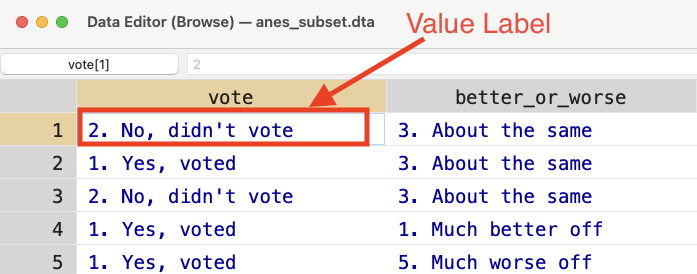
\includegraphics[width=0.75\linewidth]{images/05_br2} 

}

\caption{Browsing the ANES}\label{fig:br2value}
\end{figure}

The \textbf{value label} is the text highlighted in blue (``2. No, didn't vote''). If we use \texttt{tab} we can see the different values labels for a given variable. Let's try this for \texttt{vote}:

\begin{Shaded}
\begin{Highlighting}[]
\KeywordTok{tab}\NormalTok{ vote }
\NormalTok{file gapminder.dta }\KeywordTok{not}\NormalTok{ Stata }\KeywordTok{format}
\FunctionTok{r}\NormalTok{(610);}


\NormalTok{no variables defined}
\FunctionTok{r}\NormalTok{(111);}

\FunctionTok{r}\NormalTok{(111);}
\end{Highlighting}
\end{Shaded}

So there are 4 different value labels. If you need to reference values of these variables, you need to use the actual numeric values, not the labels themselves. The labels are just there so we don't forget what the numbers mean. For example, if I wanted to see how many individuals refused the question, I can type:

\begin{Shaded}
\begin{Highlighting}[]
\FunctionTok{count} \KeywordTok{if}\NormalTok{ vote=={-}9}
\NormalTok{file gapminder.dta }\KeywordTok{not}\NormalTok{ Stata }\KeywordTok{format}
\FunctionTok{r}\NormalTok{(610);}


\NormalTok{vote }\KeywordTok{not}\NormalTok{ found}
\FunctionTok{r}\NormalTok{(111);}

\FunctionTok{r}\NormalTok{(111);}
\end{Highlighting}
\end{Shaded}

If I try to do the same thing, but referencing the value label, I will get an error:

\begin{Shaded}
\begin{Highlighting}[]
\FunctionTok{count} \KeywordTok{if}\NormalTok{ vote == }\StringTok{"{-}9. Refused"}
\NormalTok{file gapminder.dta }\KeywordTok{not}\NormalTok{ Stata }\KeywordTok{format}
\FunctionTok{r}\NormalTok{(610);}


\NormalTok{vote }\KeywordTok{not}\NormalTok{ found}
\FunctionTok{r}\NormalTok{(111);}

\FunctionTok{r}\NormalTok{(111);}
\end{Highlighting}
\end{Shaded}

It states \texttt{type\ mismatch} because \texttt{vote} is a numeric variable, not a string variable. A quick way to see the numeric values associated with the labels is to type:

\begin{Shaded}
\begin{Highlighting}[]
\KeywordTok{tab}\NormalTok{ vote, }\KeywordTok{sum}\NormalTok{(vote)}
\NormalTok{file gapminder.dta }\KeywordTok{not}\NormalTok{ Stata }\KeywordTok{format}
\FunctionTok{r}\NormalTok{(610);}


\NormalTok{no variables defined}
\FunctionTok{r}\NormalTok{(111);}

\FunctionTok{r}\NormalTok{(111);}
\end{Highlighting}
\end{Shaded}

\textbf{Concept Check}

Make sure you understand why the above code can retrieve the numeric value associated with each label. Remember, \texttt{tab} creates a table of frequencies, while \texttt{sum} generates summary statistics.

\section{Missing Values}\label{missing-values}

Continuing our exploration of the ANES dataset, we will now discuss missing values. For numeric variables, Stata stores missing values as a period. If your numeric variable does not code missing information as a period, then you should change this before continuing the analysis. To see why, let's consider the variable \texttt{better\_or\_worse}, which asks the respondent on a scale of 1 to 5 how much worse off are you relative to a year ago.

\begin{Shaded}
\begin{Highlighting}[]
\KeywordTok{tab}\NormalTok{ better\_or\_worse}
\end{Highlighting}
\end{Shaded}

\begin{verbatim}
file gapminder.dta not Stata format
r(610);


no variables defined
r(111);

r(111);
\end{verbatim}

You can see that -8 and -9 are actually missing values, but right now they are stored as numbers. If I take the average of \texttt{better\_or\_worse}, I get:

\begin{Shaded}
\begin{Highlighting}[]
\KeywordTok{sum}\NormalTok{ better\_or\_worse}
\end{Highlighting}
\end{Shaded}

\begin{verbatim}
file gapminder.dta not Stata format
r(610);


no variables defined
r(111);

r(111);
\end{verbatim}

But this average incorporates those values of -9 and -8. In terms of the scale of the variable, this will lower the overall average, which could lead to some pretty misleading results. For example, imagine instead of storing the missing values as -9, they were stored as -1000. Then, even though there are a few individuals with missing data, our average value of \texttt{better\_or\_worse} might be very low, as low as 1. If we naively took this as the average, then we might conclude that on average, people report they are much better off. But this is the wrong conclusion, we need the average response among individuals that actually answered the question.

What we need to do is replace individuals that have either a value of -8 or -9 to missing. To do this we can make use of the or operator, which is given by the symbol \texttt{\textbar{}}. The code below will replace the value of \texttt{better\_or\_worse} to missing if the current value is either -8 \textbf{or} -9.

\begin{Shaded}
\begin{Highlighting}[]
\KeywordTok{replace}\NormalTok{ better\_or\_worse=. }\KeywordTok{if}\NormalTok{ better\_or\_worse=={-}8 | better\_or\_worse=={-}9}
\end{Highlighting}
\end{Shaded}

Now when we take the average, the missing values are not incorporated

\begin{Shaded}
\begin{Highlighting}[]
\KeywordTok{sum}\NormalTok{ better\_or\_worse}
\end{Highlighting}
\end{Shaded}

\begin{verbatim}
file gapminder.dta not Stata format
r(610);


no variables defined
r(111);

r(111);
\end{verbatim}

When you compute summary statistics or run regressions, observations with missing values will be dropped automatically from this calculation. However, you need to be very careful when constructing new variables from observations with missing values. For logical statements in Stata (such as when creating indicator variables), the missing value is interpreted as infinity. The reason why it was chosen to have missing values be interpreted as infinity is a little complicated, but it can lead to some confusing errors!

To see how, imagine we want to create an indicator that is equal to 1 if an individual thinks their life has gotten worse relative to 1 year ago. An individual that responded 4 or 5 believes their life has gotten worse relative to 1 year ago. So one potential way to code this new variable would be to type:

\begin{Shaded}
\begin{Highlighting}[]
\KeywordTok{gen}\NormalTok{ worse\_off = (better\_or\_worse\textgreater{}=4)}
\end{Highlighting}
\end{Shaded}

Let's see what \texttt{worse\_off} is equal to for individuals that had missing values for \texttt{better\_or\_worse}.

\begin{Shaded}
\begin{Highlighting}[]
\KeywordTok{sum}\NormalTok{ worse\_off }\KeywordTok{if}\NormalTok{ better\_or\_worse==.}
\end{Highlighting}
\end{Shaded}

\begin{verbatim}
file gapminder.dta not Stata format
r(610);


no variables defined
r(111);

r(111);
\end{verbatim}

It is equal to 1 for all of these individuals, but why? The reason is missing values are interpreted as infinity in logical statements. Because infinity is greater than 4, then everyone with missing values of this is coded as \texttt{worse\_off=1}.

To avoid this problem, we need to change the code so that it takes into account the possibility of missing values. For example, we might want to replace \texttt{worse\_off} equal to missing if \texttt{better\_or\_worse} is equal to missing.

\begin{Shaded}
\begin{Highlighting}[]
\KeywordTok{replace}\NormalTok{ worse\_off = . }\KeywordTok{if}\NormalTok{ better\_or\_worse==.}
\end{Highlighting}
\end{Shaded}

\section{Binned Scatterplots (Theory)}\label{binned-scatterplots-theory}

In this chapter, we will discuss a new data visualization technique known as \textbf{binned scatterplots}. To understand this technique, let's first take a simple example. Imagine, we have the dataset below in Figure \ref{fig:barill} which shows Earnings (vertical axis) against test scores (horizontal axis):

\begin{figure}

{\centering 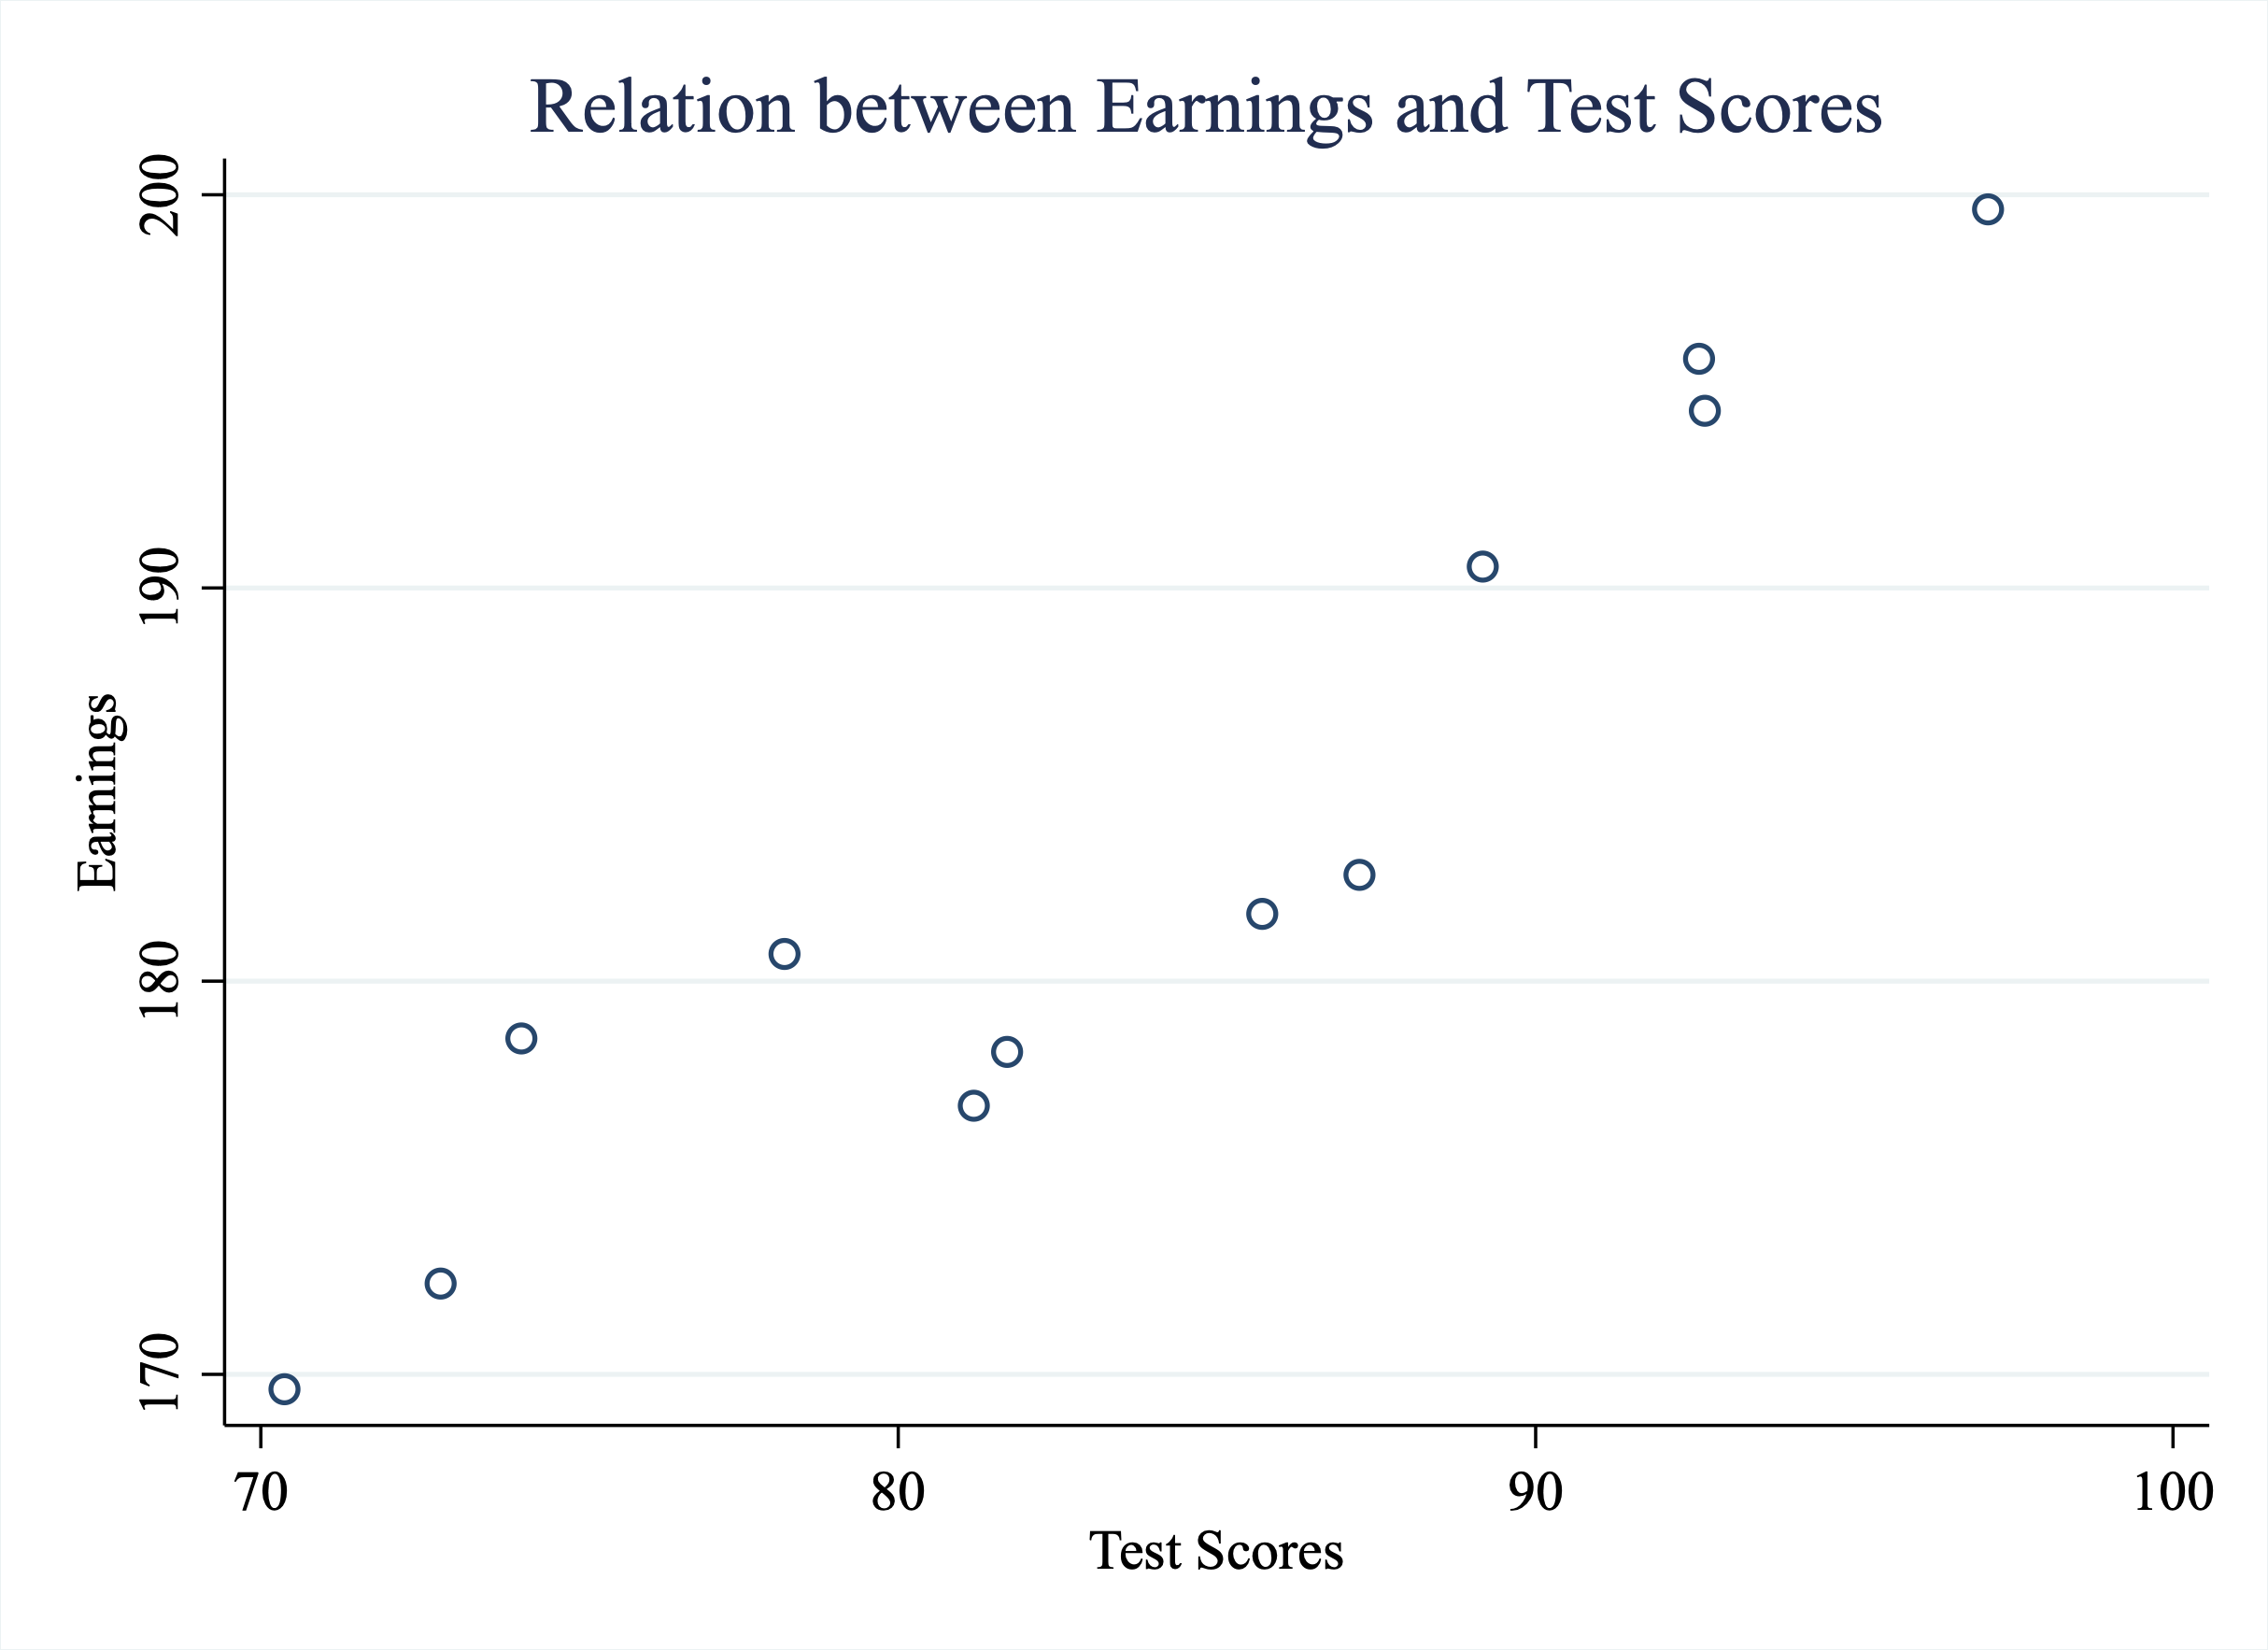
\includegraphics[width=0.65\linewidth]{images/05_bin1} 

}

\caption{Relationship Between Earnings and Test Scores}\label{fig:barill}
\end{figure}

In this example, we have plotted all the data and can clearly see that there is a positive relationship between test scores and earnings. Individuals with higher test scores tend to also have higher earnings. But what if there were 1,000 people in this dataset, or 10,000, or a million? The graph would soon get pretty crowded. Not only would a graph with a million observations be difficult to interpret, but it would also likely crash your computer!

However, instead of plotting all the data, imagine we bin the data into intervals. For example, in Figure \ref{fig:barill2} we have binned the data into intervals by dividing the x-axis into three bins. In bin 1 there are observations with scores below 80. Bin 2 has observations with scores between 80 and 90. Bin 3 has scores above 90.

\begin{figure}

{\centering 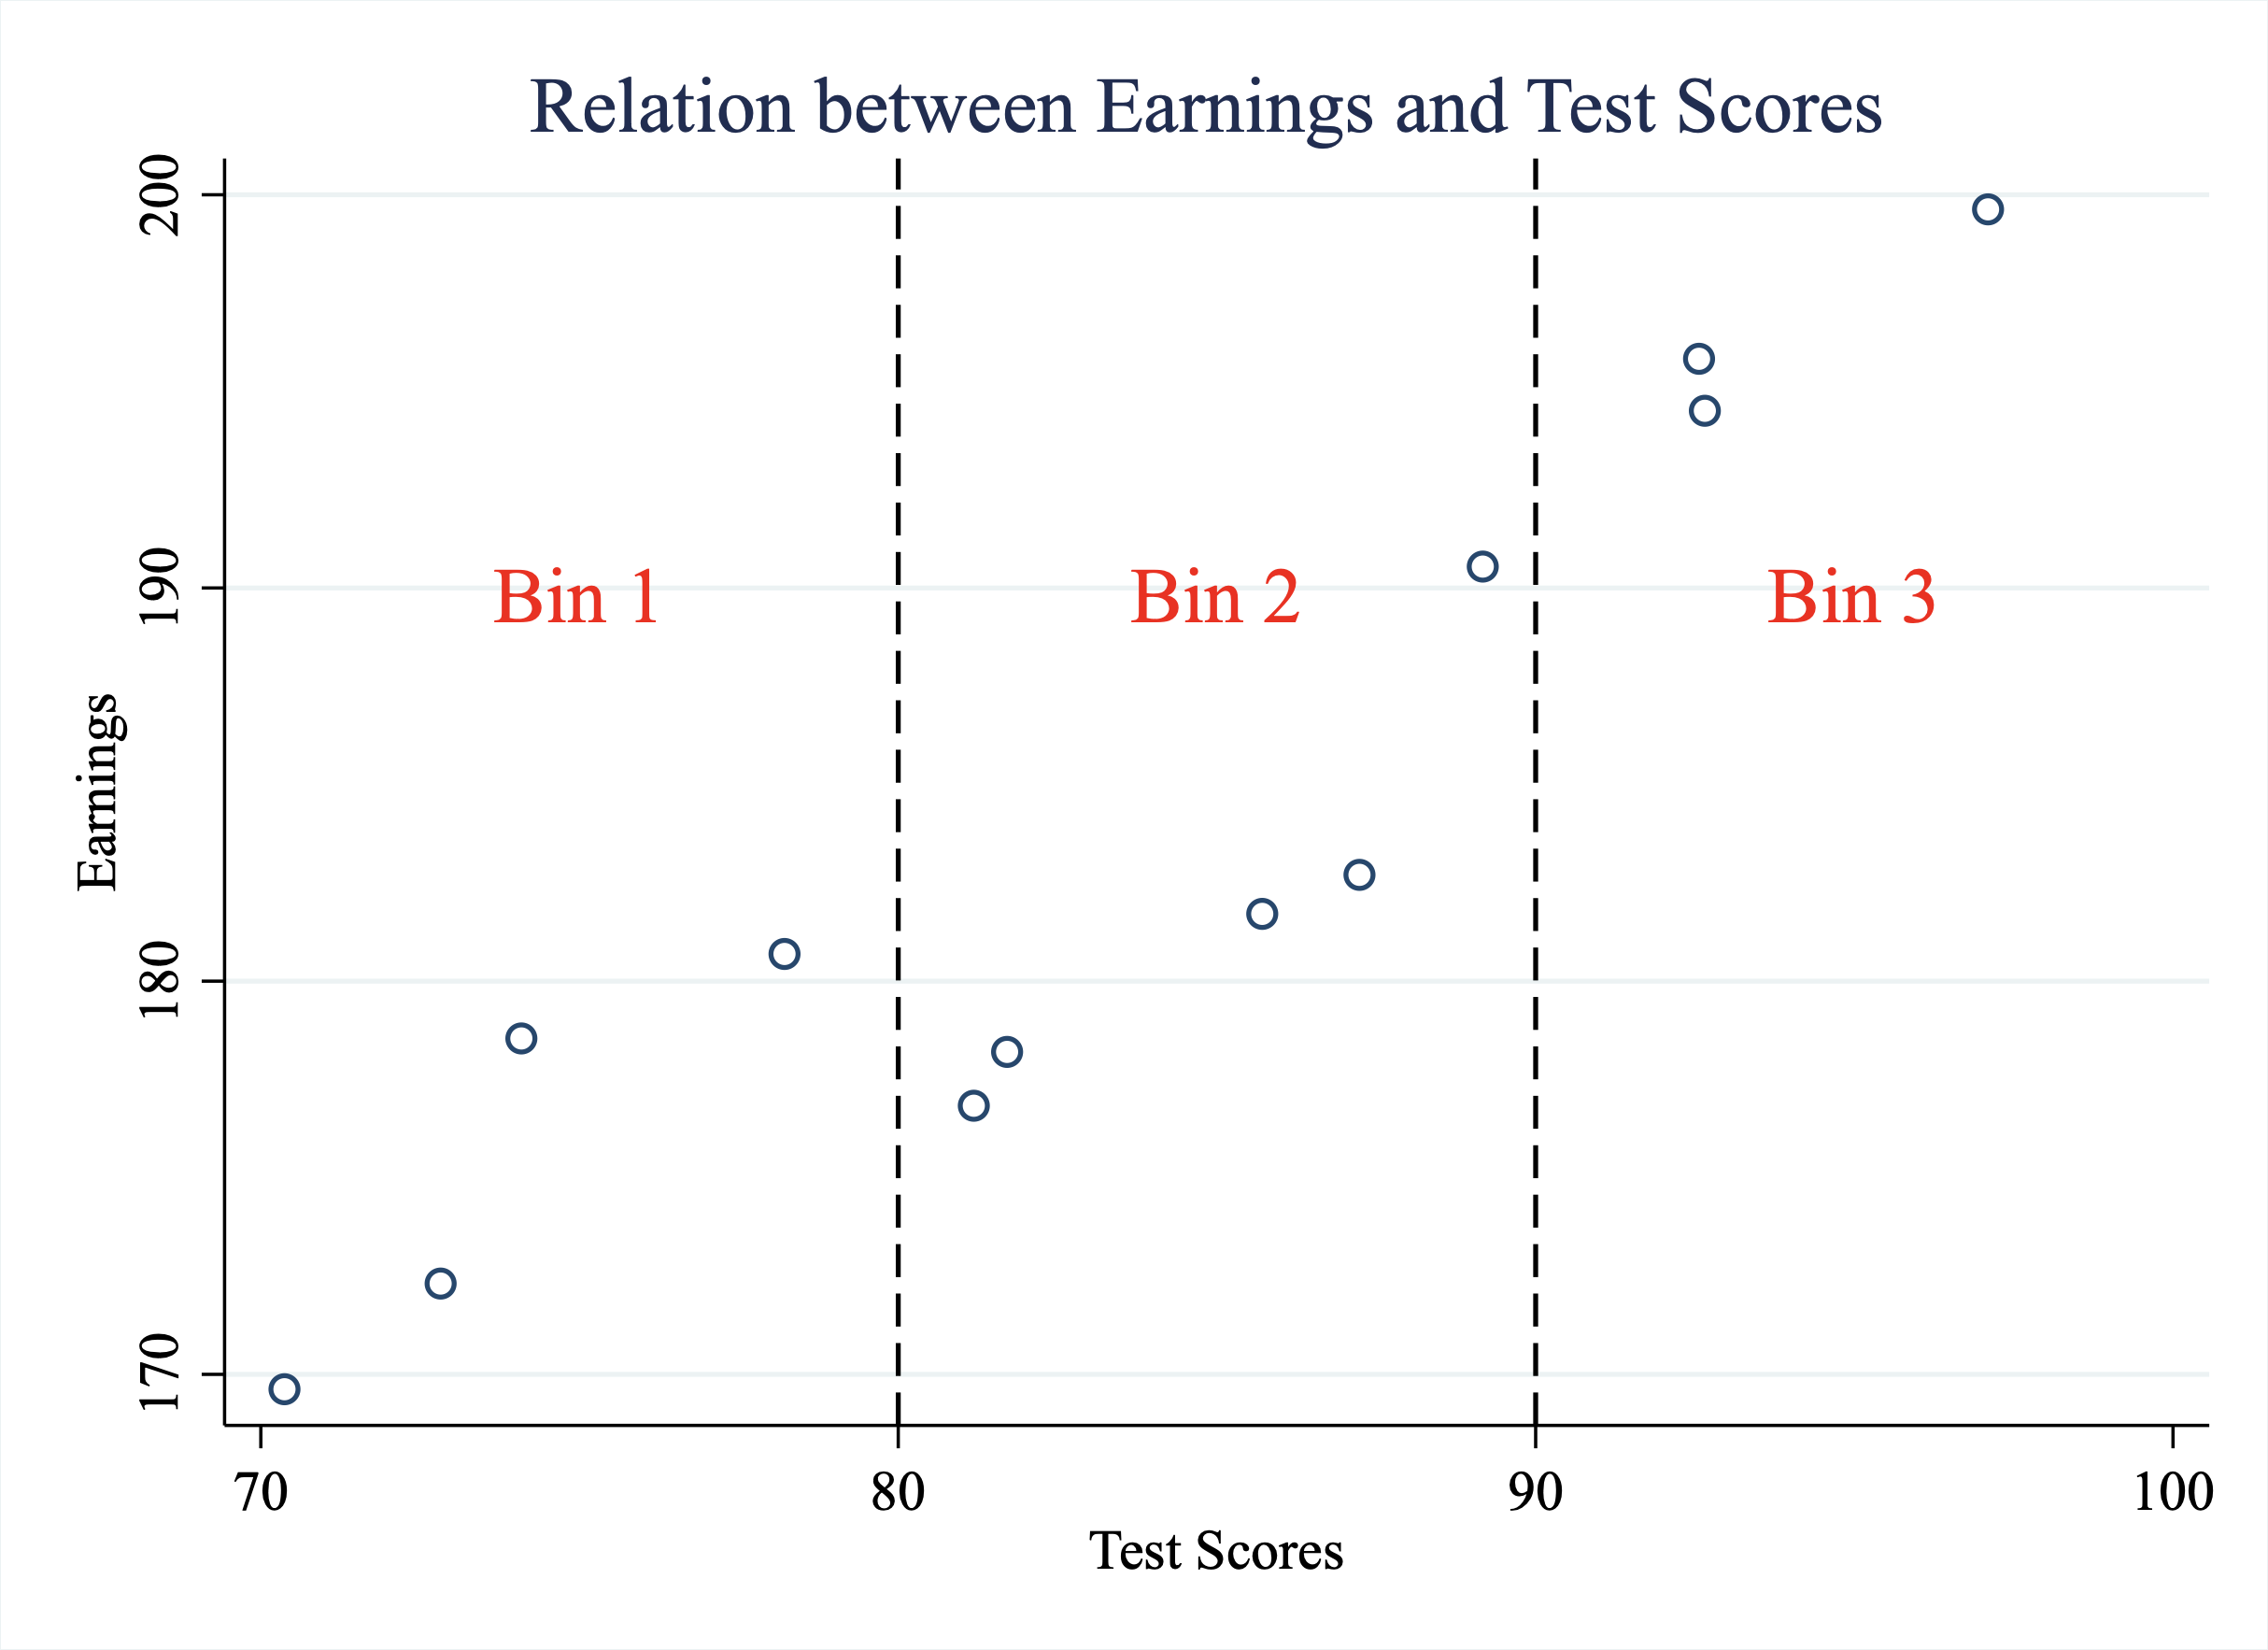
\includegraphics[width=0.65\linewidth]{images/05_bin2} 

}

\caption{Binning the Data}\label{fig:barill2}
\end{figure}

Now instead of plotting all the data, let's just plot the averages within each bin, as depicted in Figure \ref{fig:barill3}

\begin{figure}

{\centering 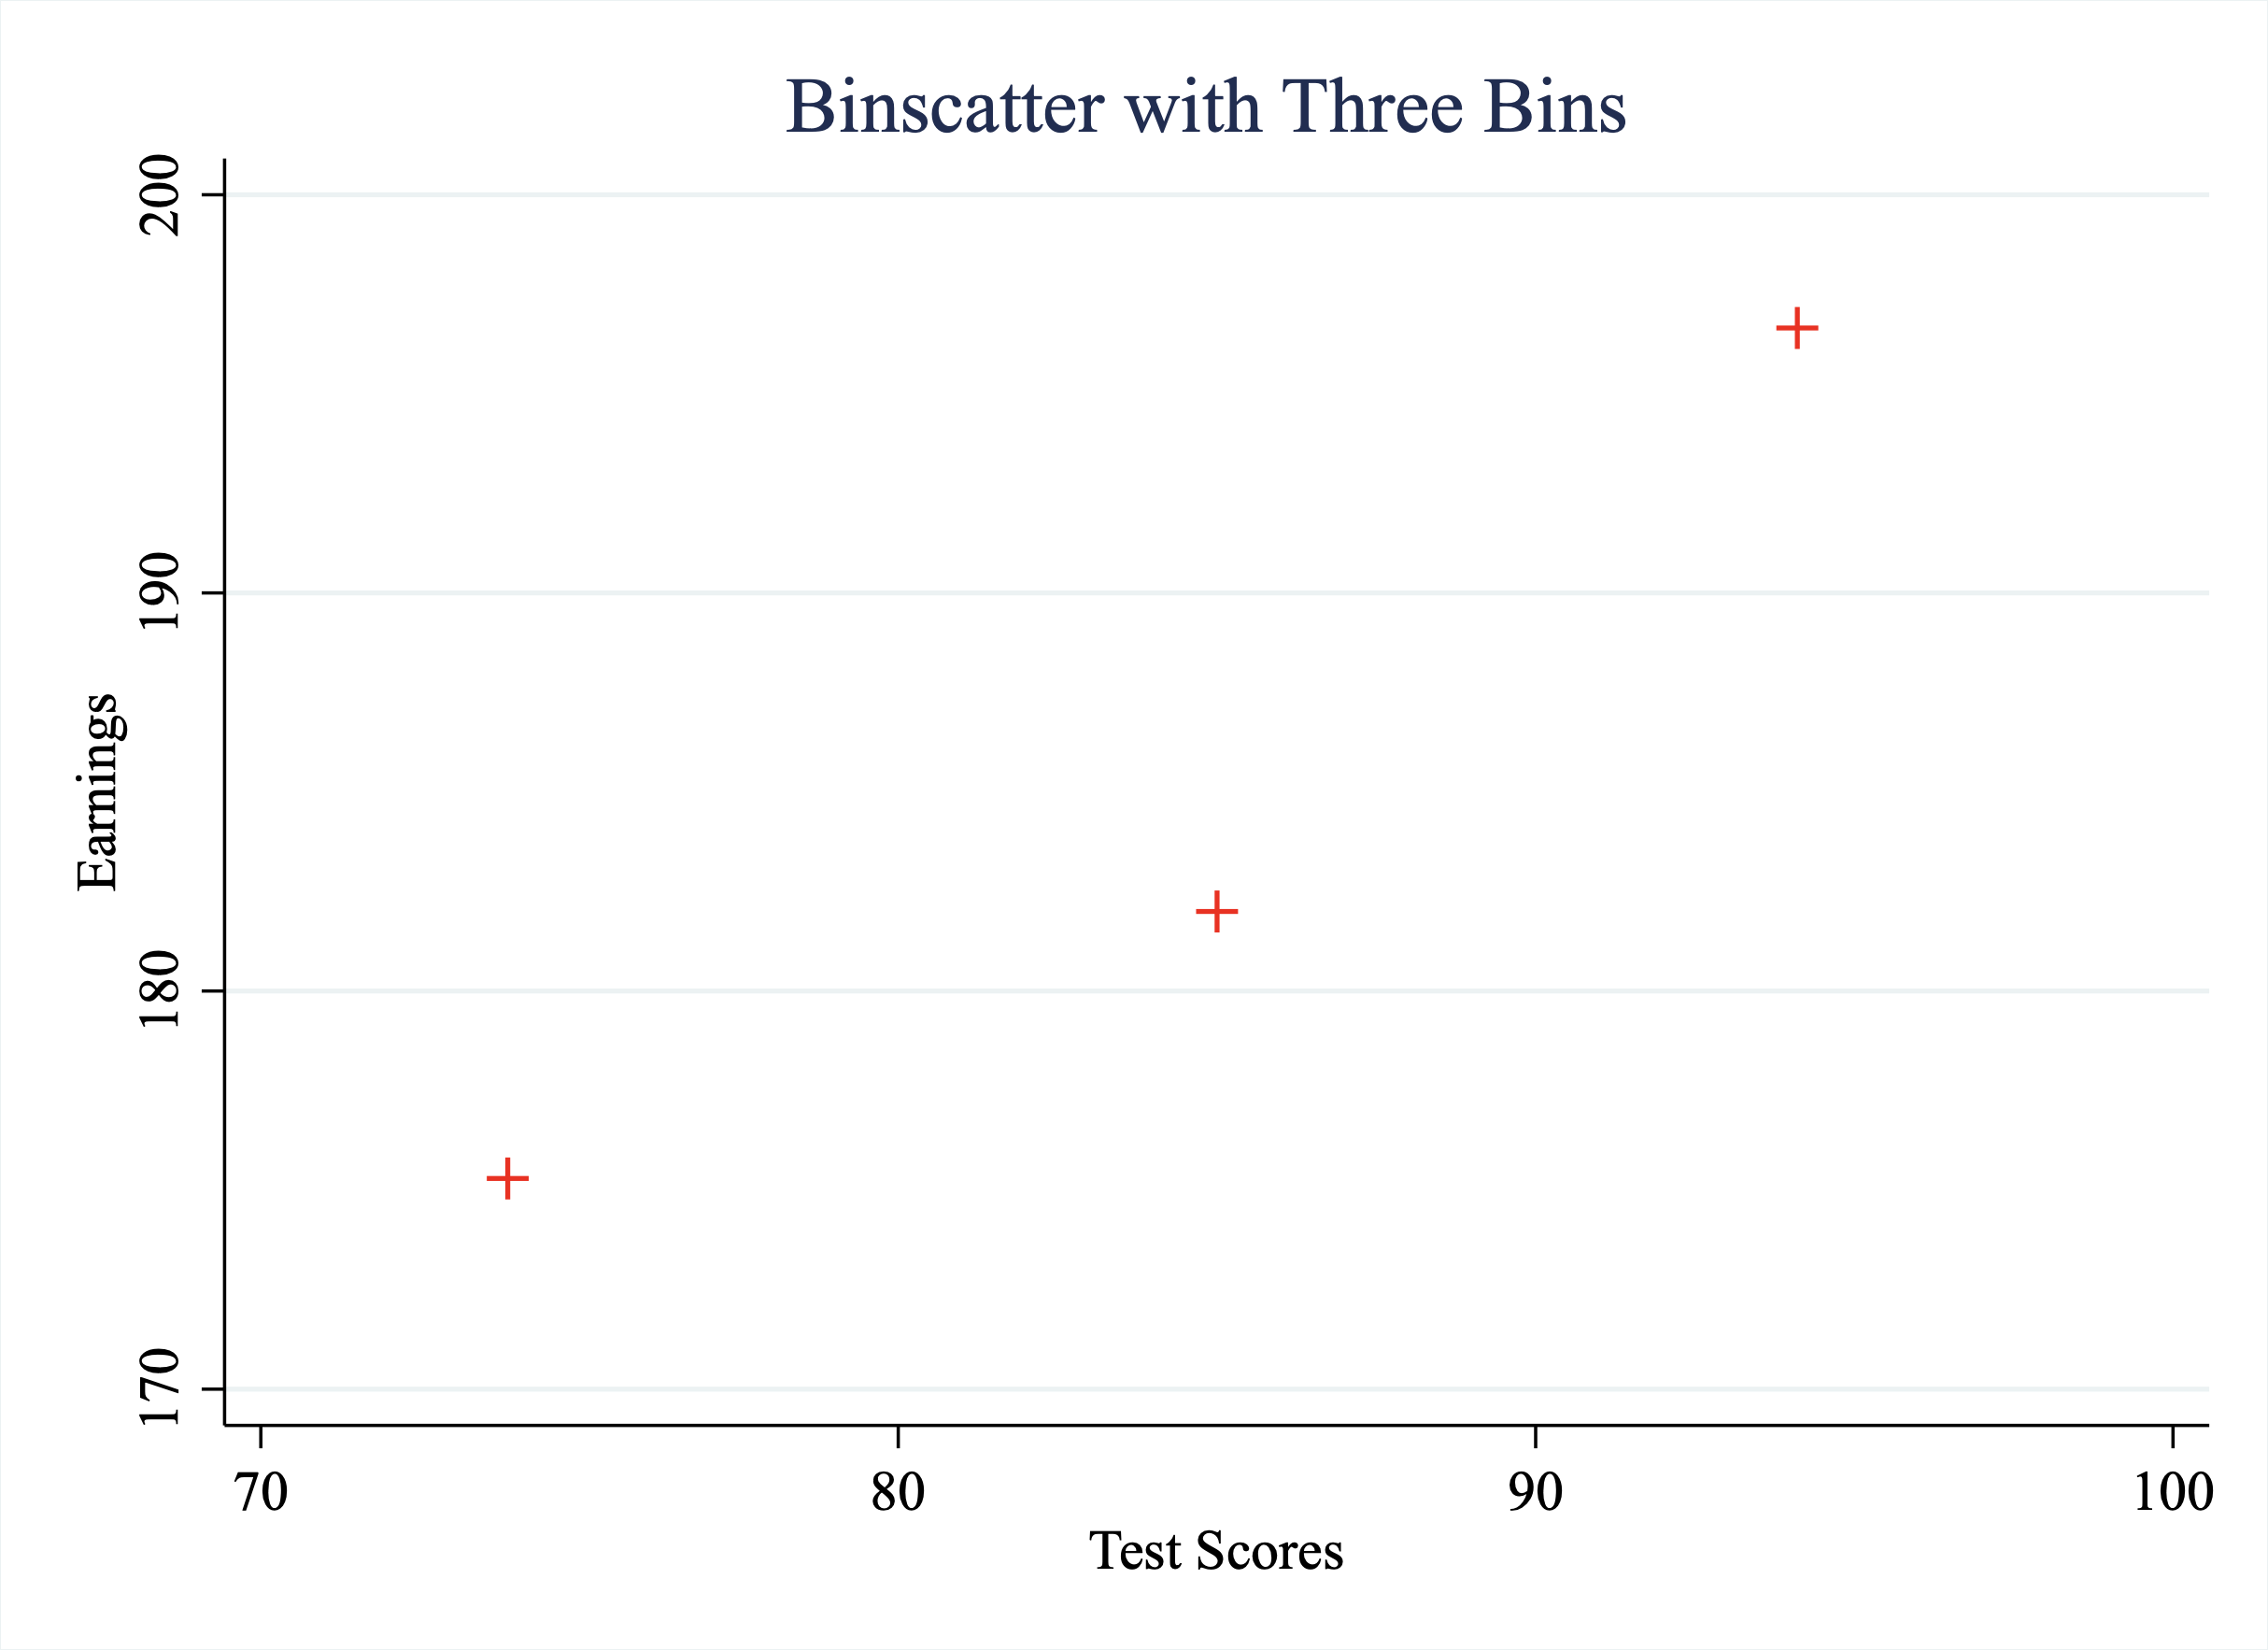
\includegraphics[width=0.65\linewidth]{images/05_bin4} 

}

\caption{An Example of a Binned Scatterplot}\label{fig:barill3}
\end{figure}

This binned scatterplot allows us to transparently observe the relationship between two variables. However, now imagine we had 1000 students instead of the original 12. Well, the binned scatter plot will still have only 3 points. Note the decision to bin the data into three intervals was merely for illustrative purposes. In general, you can decide on how many bins to create. The key here is that even if the sample size grows, we can still show the relationship between these two variables in a binned scatterplot. Even if our sample size grows to a million, the number of points in the graph is still determined by the number of bins.

\section{Binned Scatterplots (Stata)}\label{binned-scatterplots-stata}

In this section, we will use the data from Lowes and Montero (2021) to implement a binned scatterplot to study the legacy of colonial medicine in Africa. In order to construct the binned scatterplot we will make use of the \texttt{binscatter} command.

As a reminder, between 1921 and 1956, French colonies in Africa were visited by many medical campaigns often forcing medical care with questionable efficacy and severe side effects. Some places were visited only a small fraction of the years. Other places were visited often in these years. Are people who lived in places with many medical campaigns more likely to distrust medicine today?

To begin let's load the dataset:

\begin{Shaded}
\begin{Highlighting}[]
\NormalTok{cd }\StringTok{"/Users/davidarnold/Dropbox/Teaching/EP5/online/05\_week/data"}
\KeywordTok{use}\NormalTok{ colonial\_medicine.dta, }\KeywordTok{replace}
\NormalTok{file gapminder.dta }\KeywordTok{not}\NormalTok{ Stata }\KeywordTok{format}
\FunctionTok{r}\NormalTok{(610);}


\NormalTok{/Users/davidarnold/Dropbox/Teaching/EP5/online/05\_week/}\KeywordTok{data}
\end{Highlighting}
\end{Shaded}

First, we need to drop values that either have missing information for \texttt{refused\_any\_blood\_test} or \texttt{Times\_Prospected}. \texttt{refused\_any\_blood\_test} is our key outcome and is equal to 1 if the individual refused the free blood test and zero otherwise. \texttt{Times\_Prospected} is our key explanatory variable and captures what fraction of years between 1921-and 1956 was the individual's region visited for sleeping sickness campaigns. If either of these values are missing for an observation, then they should not be included in the analysis.

\begin{Shaded}
\begin{Highlighting}[]
\KeywordTok{drop} \KeywordTok{if}\NormalTok{ refused\_any\_blood\_test==. | Times\_Prospected==. }
\NormalTok{file gapminder.dta }\KeywordTok{not}\NormalTok{ Stata }\KeywordTok{format}
\FunctionTok{r}\NormalTok{(610);}


\NormalTok{refused\_any\_blood\_test }\KeywordTok{not}\NormalTok{ found}
\FunctionTok{r}\NormalTok{(111);}

\FunctionTok{r}\NormalTok{(111);}
\end{Highlighting}
\end{Shaded}

The parallel line \texttt{\textbar{}} indicates ``or''. So put simply, this line says to drop any observations in which either \texttt{refused\_any\_blood\_test} or \texttt{Times\_Prospected} is missing.

Next, we will use an external command named \texttt{binscatter} can be used to produce binned scatterplots. To install on your version of Stata, you first need to type.

\begin{Shaded}
\begin{Highlighting}[]
\KeywordTok{ssc}\NormalTok{ install binscatter}
\end{Highlighting}
\end{Shaded}

Once you execute the code above once, then you will be able to use the \texttt{binscatter} command. The basic syntax of the \texttt{binscatter} command is:

\begin{Shaded}
\begin{Highlighting}[]
\NormalTok{binscatter yvar xvar, nquantiles(\#)}
\end{Highlighting}
\end{Shaded}

In this syntax, you will replace \texttt{yvar} with whatever variable you want to plot on the vertical axis and \texttt{xvar} with whatever variable you want to plot on the horizontal axis. You will replace \texttt{\#} with however many bins you want to create.

In our example, we want to understand the relationship between refusing to take a blood test (y-axis) and share of years visited by medical campaigns between 1921-1956 (x-axis). For illustrative purposes, let's specify \texttt{nquantiles(10)} which implies we will have 10 bins in our scatterplot. One nice thing about the \texttt{binscatter} command is that we can utilize everything that we've learned from creating graphs generally. In other words, let's make sure our graph has appropriate titles and axes labels.

\begin{Shaded}
\begin{Highlighting}[]
\NormalTok{binscatter refused\_any\_blood\_test Times\_Prospected, nq(10)  }\CommentTok{///}
    \BaseNTok{title}\NormalTok{(}\StringTok{"Binscatter: Refusing Blood Test vs. Share of Years Visited"}\NormalTok{) }\CommentTok{///}
    \BaseNTok{xtitle}\NormalTok{(}\StringTok{"Share of years visited, 1921{-}1956"}\NormalTok{) }\CommentTok{///}
    \BaseNTok{ytitle}\NormalTok{(}\StringTok{"Refused any blood test"}\NormalTok{)}
\end{Highlighting}
\end{Shaded}

\begin{figure}

{\centering 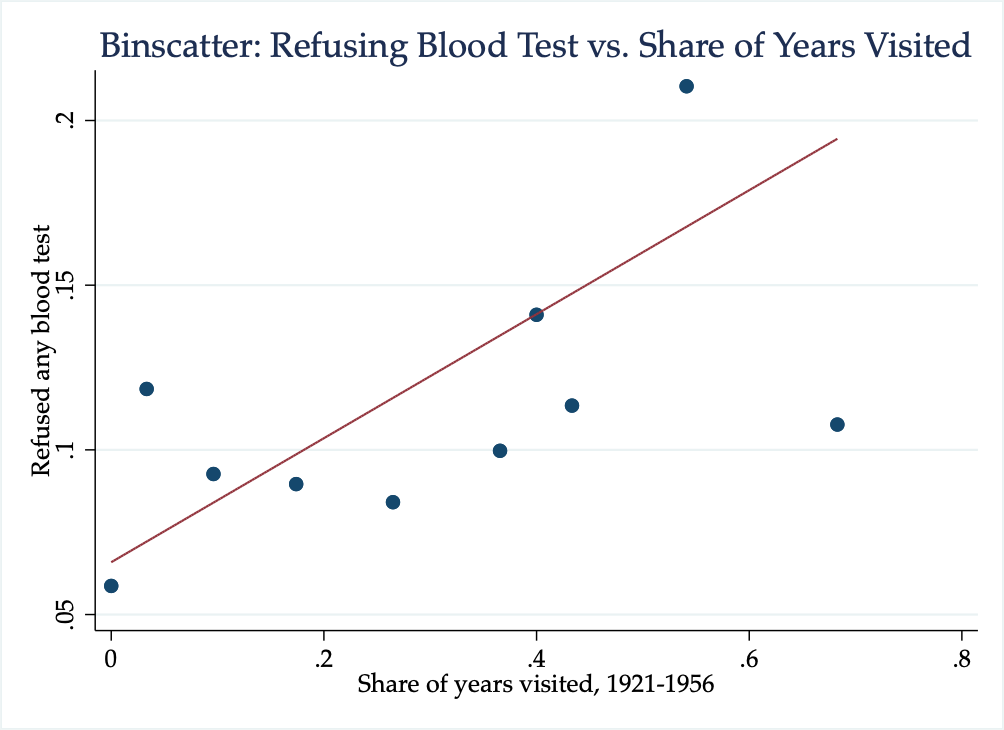
\includegraphics[width=0.65\linewidth]{images/05_binscatter2} 

}

\caption{Binscatter: Refusing Blood Test vs. Share of Years Visited}\label{fig:binscatter1}
\end{figure}

As we can see from the graph, as the share of years visited increases, the fraction of individuals who refuse a blood test also increases. This provides supporting evidence for the initial hypothesis: areas that have a history of colonial medicine still distrust medicine today. The line depicted in the binned scatterplot is a regression line that shows the strength of this relationship.

It is also helpful for interpretation to retrieve the slope of this regression line. We can get this parameter by specifying \texttt{reportreg} as an option for our binscatter command.

\begin{Shaded}
\begin{Highlighting}[]
\NormalTok{binscatter refused\_any\_blood\_test Times\_Prospected, nq(10) reportreg }
\end{Highlighting}
\end{Shaded}

\begin{figure}

{\centering 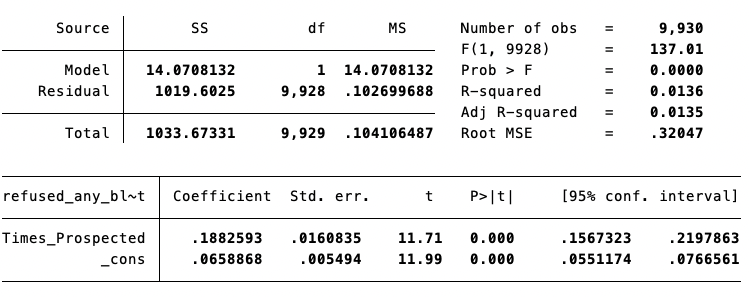
\includegraphics[width=0.85\linewidth]{images/05_binreg} 

}

\caption{Regression Line: Refusing Blood Test vs. Share of Years Visited}\label{fig:reglinebin}
\end{figure}

\textbf{Concept Check}

From this regression line, we can conclude that an increase in 7 years of medical campaign visits is associated with a 3.8 percentage point increase in the rate of blood test refusal. If you understand (1) the scale of the variables and (2) the slope coefficient, you should be able to convince yourself this is true.

Hint: Remember that a 1-unit change in the X-variable is associated with a \(\beta\)-unit change in the Y-variable. The hardest thing about this problem is understanding the units of the X and Y variables in this example.

\section{Conclusion}\label{conclusion-3}

In this final section, we will summarize what we have learned so far and then present additional results from Lowes and Montero (2021). The goal of Lowes and Montero (2021) is to understand how medical campaigns in Africa between 1921 and 1956 impact perceptions of medicine today. Colonial medical campaigns undertaken to prevent sleeping sickness often forced medical treatment. The treatments both had questionable efficacy and came with severe side effects. Lowes and Montero (2021) utilize newly digitized French military records in order to measure the exposure of a region to medical campaigns in the past, and combine this information with health surveys to understand the impact of past campaigns on health behaviors today.

What we have explored is how exposure to these campaigns impacted the choice to refuse a blood test. While this blood test was free to survey participants and had an overall high takeup, some individuals rejected the blood test. This could be one proxy for trust in modern medicine. We found in the prior section that areas with more exposure to medical campaigns were more likely to refuse the blood test.

One thing you may notice if you read Lowes and Montero (2021), however, is that our results don't appear exactly the same as those in Lowes and Montero (2021). One reason is that Lowes and Montero (2021) also control for other potential factors that could be correlated with historical exposure to medical campaigns as well as health behaviors today. Maybe places with more exposure to colonial medical campaigns vary along a number of dimensions, and these other dimensions could explain the correlation we found. Turns out, you can estimate binned scatterplots that control for other factors. Doing so goes beyond this course, but in Lowes and Montero (2021) the authors control for other factors that impact health decisions, such as age, gender, urban-rural status, among others. Figure \ref{fig:lm1} displays the binned scatterplot we constructed while also controlling for these factors.

\begin{figure}

{\centering 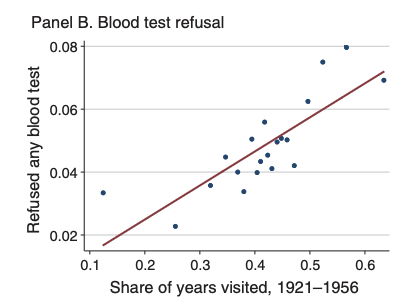
\includegraphics[width=0.65\linewidth]{images/05_lm_1} 

}

\caption{Binscatter: Refusing Blood Test vs. Share of Years Visited}\label{fig:lm1}
\end{figure}

Lowes and Montero (2021) also study if colonial medical campaigns impact vaccination rates today. To do so, they construct a vaccination index, which is the share of completed vaccines (out of 9) for children under 5. Again, they found places with more years of colonial medical visits have lower vaccination rates, as shown in Figure \ref{fig:lm2}.

\begin{figure}

{\centering 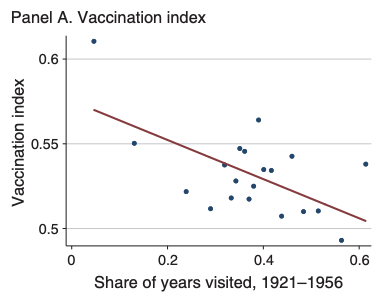
\includegraphics[width=0.65\linewidth]{images/05_lm_2} 

}

\caption{Binscatter: Vaccination vs. Share of Years Visited}\label{fig:lm2}
\end{figure}

This paper finds that negative experiences in the past were transmitted across generations. This finding has important implications for trust in institutions generally. It also has very real policy implications. Lowes and Montero (2021) find World Bank projects related to health are less successful in areas with high exposure to colonial medicine.

\section*{Command Descriptions}\label{command-descriptions-2}
\addcontentsline{toc}{section}{Command Descriptions}

\textbf{Commands Descriptions}

\begin{itemize}
\tightlist
\item
  \texttt{binscatter\ yvar\ xvar,\ nquantiles(\#)} - creates a binned scatter plot with \texttt{yvar} on the vertical axis, \texttt{xvar} on the horizontal axis. \texttt{nquantiles(\#)} determines how many bins will be created in the final scatter plot. For example \texttt{nquantiles(10)} specifies 10 bins.
\end{itemize}

\textbf{More Concepts}

\begin{itemize}
\item
  value labels - a value label is a string text associated with the particular numeric value of a variable. This is often useful for categorical variables. Having the variable be numeric allows you to perform mathematical operations on the variable, but having a label lets you easily interpret what each numeric value represents.
\item
  missing values - a missing value for a numeric variable in Stata is stored as a period. Be careful about using relations with respect to missing variables. For example, imagine you want to create a binary indicator that is equal to 1 if an individual is above the age of 40. You might type \texttt{gen\ above\_40\ =\ (age\textgreater{}40)}. If there are individuals with ages that are missing, then \texttt{above\_40} will be equal to 1 for these individuals. To replace it back to missing, you can type \texttt{replace\ above\_40\ =\ .\ if\ age==.}.
\end{itemize}

\part{R}\label{part-r}

\chapter{Resume Experiments}\label{resume-experiments}

\section{Correspondence Studies}\label{correspondence-studies}

The motivation for this week's empirical application is the pervasive evidence of inequality in the labor market. For example, Black workers are about twice as likely as white workers to be unemployed (Council of Economic Advisors, 1998). However, it is often difficult to isolate discrimination from employers as a source of a given disparity. For example, some argue researchers do not have all factors that go into an employer's decision to hire a worker, therefore differences in hiring rates across different races could be due to these other factors that are unobserved.

This week we will be studying an extremely clever method for identifying discrimination in the labor market: resume audit studies, also known as correspondence studies. The paper we will be studying is Bertrand and Mullainathan (2004)\citep{bertrand2004emily} sends fictitious resumes to help-wanted ads in Boston and Chicago. Their unique angle is that they manipulate the perception of race by altering the name on the resume:

\begin{itemize}
\item
  Examples of white-sounding names from the paper: Emily Walsh and Greg Baker
\item
  Examples of Black-sounding names from the paper: Lakisha Washington and Jamal Jones
\end{itemize}

All other characteristics of the applicant (experience, education, job history) are randomized. They then compare callback rates (for an interview) between Black and white applicants.

Why is this design so clever? Well, all factors relevant to a job are held fixed by construction. Disparities in callback rates between races can no longer be ``explained away'' by other factors. The researchers themselves have generated these resumes. All factors are observed and similar between white and Black applicants by construction. Therefore, if you do find a disparity now, then this is very strong evidence for discrimination in the labor market.

Before getting to the data though, we need to learn how to use the program we will be studying for the rest of the book: R. At this point, we would also like to credit Kosuke Imai's Textbook: Quantitative Social Science: An Introduction, where this example is drawn from.\citep{imai2018quantitative}

\section{Installing R/RStudio}\label{installing-rrstudio}

In this course, we will be using R and Rstudio. R and Rstudio will work together to perform data analysis. But why two programs instead of one?

R is the software that actually does all the work. It is the software that executes functions and gives you results. Rstudio is a software that provides a nice interface through which to use R. So basically, R is the actual machinery, Rstudio is there to improve your user experience. You don't strictly need Rstudio to use R, but it helps a lot! Whenever we ``open R'' in this course, we will actually be opening RStudio.

Because RStudio doesn't work without R, the first thing we need to do is download R. To do this you can go to \url{https://cran.r-project.org/} and download the most recent version of the software. R is available for both PC and Mac users. Once you download the package you can install it by following the instructions on the installer. One part of the instructions that sometimes trips up students is that you need to decide on a location for a CRAN mirror. The general advice for this is to choose the CRAN mirror in closest physical proximity to you. This is to potentially improve the download speed and balance resources across different servers. In practice, you really don't have to worry about this decision. Any CRAN mirror will allow you to download an identical version of R.

\section{RStudio Interface}\label{rstudio-interface}

When you open RStudio, you will be greeted by the RStudio Interface depicted below in Figure \ref{fig:rstudio}

\begin{figure}

{\centering 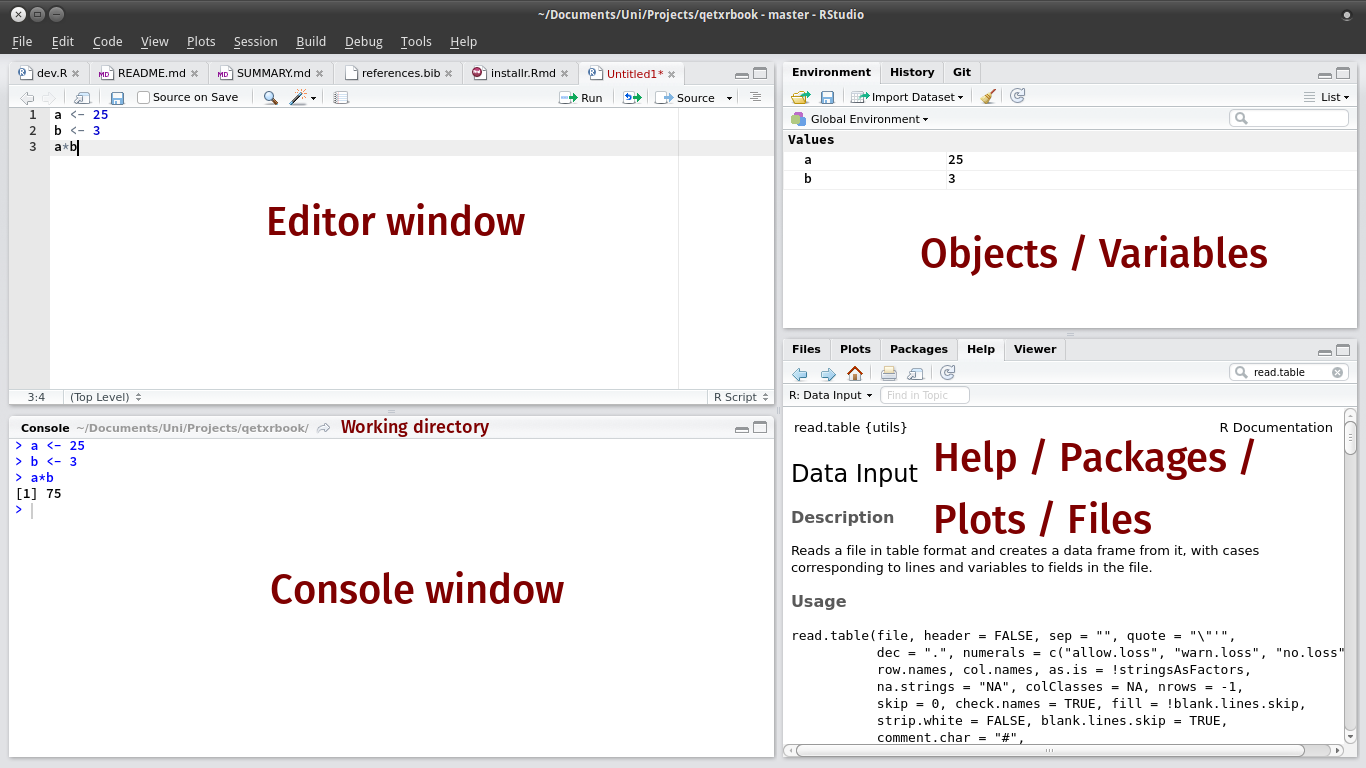
\includegraphics[width=0.9\linewidth]{images/06_rstudio} 

}

\caption{R Studio Interface}\label{fig:rstudio}
\end{figure}

Let's discuss these 4 windows in turn. In the top left is the Editor Window. This is where you will write an R script that holds all of your code. You may not see this window initially if you have not yet opened an R script (which is the equivalent to a do-file in Stata). To open up a new R script you can go to \texttt{File\ \textgreater{}\ New\ File\ \textgreater{}\ R\ Script}.

Below the Editor Window is the Console. This is where all your code will be executed and run. For example, if you write code to take the average of a variable in the Editor Window, when you execute that code, the result will be displayed in the Console.

In the top right, we have the Environment, which is going to store objects, variables, and datasets. We will get more into what an object is further into the chapter.

Lastly, the bottom right window has a host of tabs that will be helpful. One that we will use frequently is the Plots tab. This is where the figures that we create in R will be displayed. Another important tab is the Packages tab. Further in this chapter, we will discuss the importance of packages in R. Lastly, we will also use the Help tab frequently. In this tab, you can search for documentation on how to use certain functions in R. This is similar to the help files that we often used in the Stata chapters.

So now that we understand the different components of the interface, we are going to get started with coding in R. The first thing to do is open a new R script. As discussed above, to do this, you can navigate to \texttt{File\ \textgreater{}\ New\ File\ \textgreater{}\ R\ Script}.

Now, in the R script, type:

\begin{Shaded}
\begin{Highlighting}[]
\DecValTok{5}\SpecialCharTok{+}\DecValTok{3}
\end{Highlighting}
\end{Shaded}

This line of code computes the sum of 5 and 3. To execute it, you have a few options. The first way to do this is to highlight the code, then press the Run button at the top right of the Editor window.

\begin{figure}

{\centering 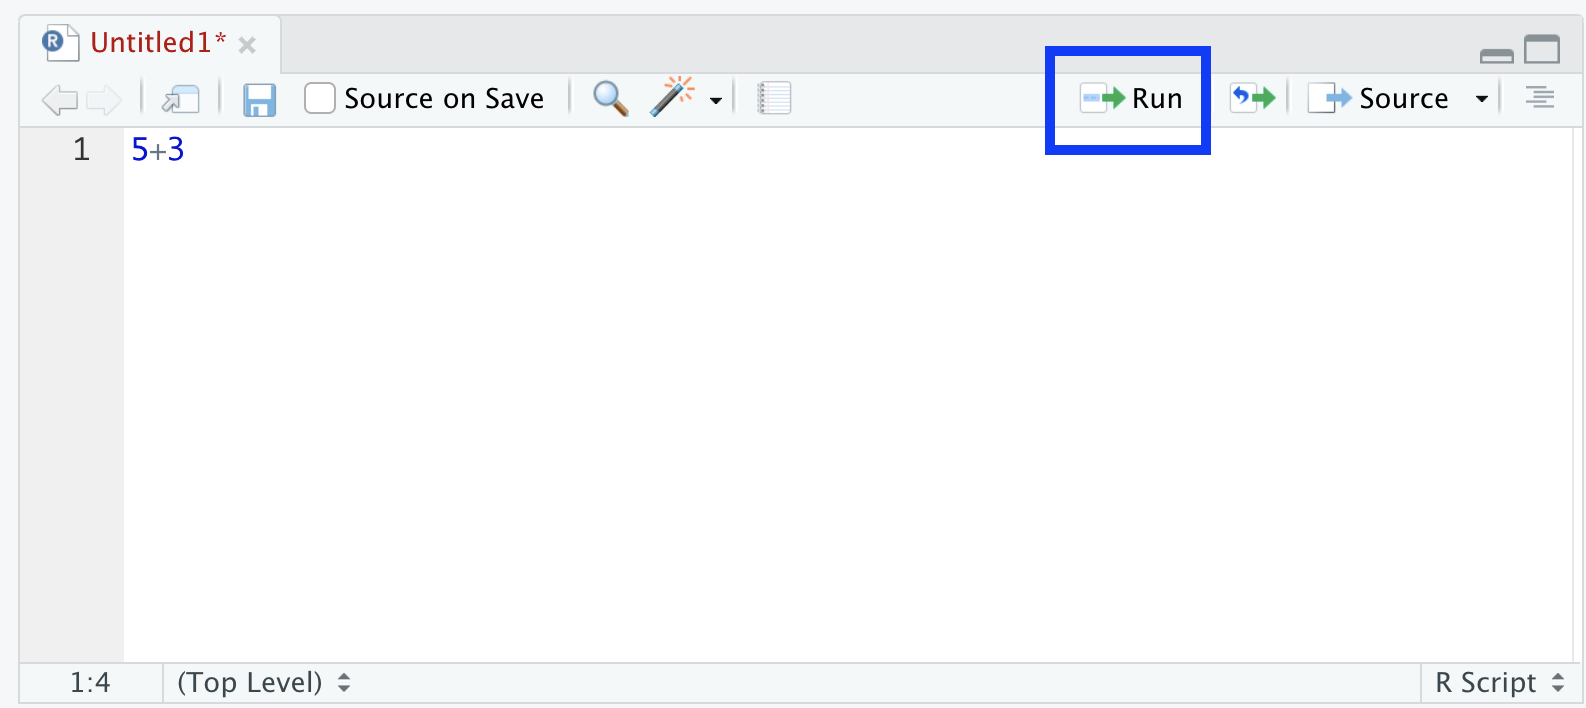
\includegraphics[width=0.9\linewidth]{images/06_run} 

}

\caption{Run Button}\label{fig:run}
\end{figure}

By clicking Run, the code is sent to the Console to be executed:

\begin{Shaded}
\begin{Highlighting}[]
\DecValTok{5}\SpecialCharTok{+}\DecValTok{3}
\NormalTok{[}\DecValTok{1}\NormalTok{] }\DecValTok{8}
\end{Highlighting}
\end{Shaded}

The other way to execute code is through using shortcuts. On a Mac, if you click on a line of code, and then press \texttt{Command\ +\ Enter}, then that line of code will be sent to the console. On a PC, this is \texttt{Ctrl\ +\ Enter}. If you want to run multiple lines, you can simply highlight the lines you want to run, and then press either \texttt{Command\ +\ Enter} or \texttt{Ctrl\ +\ Enter} and then R will execute all of those lines of code in sequential order.

Just like in Stata, you can do multiplication by using \texttt{*}, division by using \texttt{/} and exponents by using \texttt{\^{}}. In R, the order of operations is controlled by parentheses:

\begin{Shaded}
\begin{Highlighting}[]
\NormalTok{(}\DecValTok{5}\SpecialCharTok{+}\DecValTok{3}\NormalTok{)}\SpecialCharTok{/}\DecValTok{3}
\NormalTok{[}\DecValTok{1}\NormalTok{] }\FloatTok{2.666667}
\DecValTok{5} \SpecialCharTok{+} \DecValTok{3}\SpecialCharTok{/}\DecValTok{2}
\NormalTok{[}\DecValTok{1}\NormalTok{] }\FloatTok{6.5}
\end{Highlighting}
\end{Shaded}

We can also utilize more complicated mathematical functions, like the log function, square root, or absolute value:

\begin{Shaded}
\begin{Highlighting}[]
\FunctionTok{log}\NormalTok{(}\DecValTok{5}\NormalTok{)}
\NormalTok{[}\DecValTok{1}\NormalTok{] }\FloatTok{1.609438}
\FunctionTok{sqrt}\NormalTok{(}\DecValTok{2}\NormalTok{)}
\NormalTok{[}\DecValTok{1}\NormalTok{] }\FloatTok{1.414214}
\FunctionTok{abs}\NormalTok{(}\SpecialCharTok{{-}}\DecValTok{1}\NormalTok{)}
\NormalTok{[}\DecValTok{1}\NormalTok{] }\DecValTok{1}
\end{Highlighting}
\end{Shaded}

If we are ever unsure what a function does, we can utilize the help files. For example, for the log function, we may not be sure what the base is. To bring up the help file for the log function we can type:

\begin{Shaded}
\begin{Highlighting}[]
\NormalTok{?log}
\end{Highlighting}
\end{Shaded}

Reading the help file will inform us that by default, the base of the log function is equal to \(e\), which implies the default is to take the natural logarithm. Additionally, the help file tells you how to compute logarithms for different bases, such as base 10.

As in Stata, it will be helpful to document your code. When doing empirical projects, you want to be able to go back to the code at a later date and quickly understand what the code is doing. Comments are essential for this. Again, comments are lines within a script that are not meant to be run. They are there to describe what the code is doing.

Any line with a \texttt{\#} at the beginning is commented out. If you don't comment out descriptions of the code, then R will try to execute them, leading to errors in the output. So, for example, imagine I want to calculate the hypotenuse of a particular triangle, with sides of lengths 5 and 4. The code below does this, while also documenting what the code is doing.

\begin{Shaded}
\begin{Highlighting}[]
\CommentTok{\#Calculate the hypotenuse of a triangle}
\CommentTok{\#One side = 5}
\CommentTok{\#The other side = 4}
\CommentTok{\#The hypotenuse is:}
\FunctionTok{sqrt}\NormalTok{(}\DecValTok{5}\SpecialCharTok{\^{}}\DecValTok{2} \SpecialCharTok{+} \DecValTok{4}\SpecialCharTok{\^{}}\DecValTok{2}\NormalTok{)}
\NormalTok{[}\DecValTok{1}\NormalTok{] }\FloatTok{6.403124}
\end{Highlighting}
\end{Shaded}

Now imagine I forgot to comment out the first line of description. Let's see what happens

\begin{Shaded}
\begin{Highlighting}[]
\NormalTok{Calculate the hypotenuse of a triangle}
\CommentTok{\#One side = 5}
\CommentTok{\#The other side = 4}
\CommentTok{\#The hypotenuse is:}
\FunctionTok{sqrt}\NormalTok{(}\DecValTok{5}\SpecialCharTok{\^{}}\DecValTok{2} \SpecialCharTok{+} \DecValTok{4}\SpecialCharTok{\^{}}\DecValTok{2}\NormalTok{)}
\NormalTok{Error }\ControlFlowTok{in} \FunctionTok{parse}\NormalTok{(}\AttributeTok{text =}\NormalTok{ input)}\SpecialCharTok{:} \ErrorTok{\textless{}}\NormalTok{text}\SpecialCharTok{\textgreater{}}\ErrorTok{:}\DecValTok{1}\SpecialCharTok{:}\DecValTok{11}\SpecialCharTok{:}\NormalTok{ unexpected symbol}
\DecValTok{1}\SpecialCharTok{:}\NormalTok{ Calculate the}
              \SpecialCharTok{\^{}}
\end{Highlighting}
\end{Shaded}

It reports an error because \texttt{Calculate} is not executable code in R. By placing a \texttt{\#} at the beginning of the line, however, R will ignore this line and not try to execute it.

\section{Objects}\label{objects}

\emph{Objects} in R are any pieces of information:

\begin{itemize}
\tightlist
\item
  A number, called ``numeric'\,' in R (e.g.~\(5.23\))
\item
  A text string, called ``character'\,' in R (e.g.~``UCSD is awesome'')
\item
  A dataset (e.g.~we will look at a resume dataset soon)
\item
  Many more!
\end{itemize}

R can store objects with a name of our choice. In order to create an object, you can use the assignment operator \texttt{\textless{}-}. For example, if I want to create an object named \texttt{graduationdate}, which is equal to 2010, I would type

\begin{Shaded}
\begin{Highlighting}[]
\NormalTok{graduationdate }\OtherTok{\textless{}{-}} \DecValTok{2010}
\end{Highlighting}
\end{Shaded}

This will add to the Environment (top right window) a new object called graduation date, which is equal to 2010. Instead of the assignment operator \texttt{\textless{}-}, we can also use \texttt{=}. While it is generally suggested to use the assignment operator in R when creating objects, the equals sign will also work, as below.

\begin{Shaded}
\begin{Highlighting}[]
\NormalTok{graduationdate }\OtherTok{=} \DecValTok{2010}
\end{Highlighting}
\end{Shaded}

Now that we have this object stored in memory, every time we type the word \texttt{graduationdate}, R interprets the value of 2010. This means we can use our object in calculations. For example, to calculate the number of years between 2022 and the graduation date, we can type:

\begin{Shaded}
\begin{Highlighting}[]
\DecValTok{2022}\SpecialCharTok{{-}}\NormalTok{graduationdate}
\NormalTok{[}\DecValTok{1}\NormalTok{] }\DecValTok{12}
\end{Highlighting}
\end{Shaded}

If we assign a new value to the same object name, then we will overwrite this object (so be careful when doing so).

\begin{Shaded}
\begin{Highlighting}[]
\NormalTok{graduationdate }\OtherTok{\textless{}{-}} \DecValTok{2014}
\NormalTok{graduationdate}
\NormalTok{[}\DecValTok{1}\NormalTok{] }\DecValTok{2014}
\end{Highlighting}
\end{Shaded}

\texttt{R} can also represent other types of values as objects, such as strings of characters:

\begin{Shaded}
\begin{Highlighting}[]
\NormalTok{school }\OtherTok{\textless{}{-}} \StringTok{"UCSD"}
\end{Highlighting}
\end{Shaded}

We can use the class function to retrieve the type of object

\begin{Shaded}
\begin{Highlighting}[]
\FunctionTok{class}\NormalTok{(graduationdate)}
\NormalTok{[}\DecValTok{1}\NormalTok{] }\StringTok{"numeric"}
\FunctionTok{class}\NormalTok{(school)}
\NormalTok{[}\DecValTok{1}\NormalTok{] }\StringTok{"character"}
\end{Highlighting}
\end{Shaded}

So far, every object we have created has a single value associated with it. Next, we will discuss vectors. A \emph{vector} represents a collection of information of the same type stored in a specific order. For example, instead of the graduation date of a single individual, maybe we have information on the graduation date of four individuals. This collection of information constitutes a vector. We can create a vector in R by using the function \texttt{c()}, which stands for ``concatenate''. For example, let's create a vector of graduation dates:

\begin{Shaded}
\begin{Highlighting}[]
\CommentTok{\#Create a vector of graduation dates}
\NormalTok{graduationdate }\OtherTok{\textless{}{-}} \FunctionTok{c}\NormalTok{(}\DecValTok{2010}\NormalTok{, }\DecValTok{2009}\NormalTok{, }\DecValTok{2015}\NormalTok{, }\DecValTok{2001}\NormalTok{)}
\NormalTok{graduationdate}
\NormalTok{[}\DecValTok{1}\NormalTok{] }\DecValTok{2010} \DecValTok{2009} \DecValTok{2015} \DecValTok{2001}
\end{Highlighting}
\end{Shaded}

We can perform calculations on a vector as well. For example, for each student, let's compute the number of years between graduation and the year 2022.

\begin{Shaded}
\begin{Highlighting}[]
\CommentTok{\#Calculate years since graduation}
\DecValTok{2022} \SpecialCharTok{{-}}\NormalTok{ graduationdate}
\NormalTok{[}\DecValTok{1}\NormalTok{] }\DecValTok{12} \DecValTok{13}  \DecValTok{7} \DecValTok{21}
\end{Highlighting}
\end{Shaded}

\texttt{graduationdate} is a numeric vector, because each element is a number. We can also create character vectors, where each element is a word. For example, imagine next we want to create a vector that contains information on the school of each of our four individual students. We could type:

\begin{Shaded}
\begin{Highlighting}[]
\CommentTok{\#Create a vector of schools}
\NormalTok{school }\OtherTok{\textless{}{-}} \FunctionTok{c}\NormalTok{(}\StringTok{"UCSD"}\NormalTok{, }\StringTok{"UCB"}\NormalTok{, }\StringTok{"UCLA"}\NormalTok{, }\StringTok{"UCR"}\NormalTok{)}
\end{Highlighting}
\end{Shaded}

As in Stata, whenever you reference character values (also known as string values), you put these values in quotation marks. This lets R know that this information is composed of characters, not numbers.

One important note is that a vector cannot hold information of different types. In other words, you can't have a vector that holds both numeric and character values. For example, imagine we try to combine our two vectors using the \texttt{c()} function:

\begin{Shaded}
\begin{Highlighting}[]
\FunctionTok{c}\NormalTok{(graduationdate, school)}
\NormalTok{[}\DecValTok{1}\NormalTok{] }\StringTok{"2010"} \StringTok{"2009"} \StringTok{"2015"} \StringTok{"2001"} \StringTok{"UCSD"} \StringTok{"UCB"}  \StringTok{"UCLA"} \StringTok{"UCR"} 
\end{Highlighting}
\end{Shaded}

Now it may look like we have succeeded, but look carefully at the first few entries. Each entry is surrounded by quotation marks. R has changed the numeric entries to character entries.

Lastly, one helpful note is that we can use arithmetic operations between vectors. For example, imagine we have a vector of individual incomes and a vector of planned raises for each individual. To get to the total income after the raise, we can add these two vectors together.

\begin{Shaded}
\begin{Highlighting}[]
\CommentTok{\#Create a vector of income}
\NormalTok{income }\OtherTok{\textless{}{-}} \FunctionTok{c}\NormalTok{(}\DecValTok{65}\NormalTok{, }\DecValTok{70}\NormalTok{, }\DecValTok{20}\NormalTok{, }\DecValTok{100}\NormalTok{)}

\CommentTok{\#Create a vector of raises}
\NormalTok{raise }\OtherTok{\textless{}{-}} \FunctionTok{c}\NormalTok{(}\DecValTok{5}\NormalTok{, }\DecValTok{10}\NormalTok{, }\DecValTok{3}\NormalTok{, }\DecValTok{20}\NormalTok{)}

\CommentTok{\#Calculate current income for each person}
\NormalTok{income }\SpecialCharTok{+}\NormalTok{ raise}
\NormalTok{[}\DecValTok{1}\NormalTok{]  }\DecValTok{70}  \DecValTok{80}  \DecValTok{23} \DecValTok{120}
\end{Highlighting}
\end{Shaded}

In terms of data analysis, we can really think of vectors as a variable. Our first variable was \texttt{graduationdate}, our second variable was the \texttt{school}. Often, in data analysis, we want to compute some summary statistics of our variables. In R, there are a host of functions that help summarize numeric vectors:

\begin{itemize}
\tightlist
\item
  \texttt{length()}: length of a vector (number of elements)
\item
  \texttt{min()}: minimum value
\item
  \texttt{max()}: maximum value
\item
  \texttt{range()}: range of data
\item
  \texttt{mean()}: mean value
\item
  \texttt{sum()}: total sum of the elements
\end{itemize}

Let's try some of these out so that we can get a good sense of what these functions are doing:

\begin{Shaded}
\begin{Highlighting}[]
\CommentTok{\#Maximum income}
\FunctionTok{max}\NormalTok{(income)}
\NormalTok{[}\DecValTok{1}\NormalTok{] }\DecValTok{100}
\end{Highlighting}
\end{Shaded}

\begin{Shaded}
\begin{Highlighting}[]
\CommentTok{\#Minimum graduate date}
\FunctionTok{min}\NormalTok{(graduationdate)}
\NormalTok{[}\DecValTok{1}\NormalTok{] }\DecValTok{2001}
\end{Highlighting}
\end{Shaded}

\begin{Shaded}
\begin{Highlighting}[]
\CommentTok{\#Length of the vector income}
\FunctionTok{length}\NormalTok{(income)}
\NormalTok{[}\DecValTok{1}\NormalTok{] }\DecValTok{4}
\end{Highlighting}
\end{Shaded}

\begin{Shaded}
\begin{Highlighting}[]
\CommentTok{\#Range of graduation dates}
\FunctionTok{range}\NormalTok{(graduationdate)}
\NormalTok{[}\DecValTok{1}\NormalTok{] }\DecValTok{2001} \DecValTok{2015}
\end{Highlighting}
\end{Shaded}

\begin{Shaded}
\begin{Highlighting}[]
\CommentTok{\#Mean years since graduation}
\FunctionTok{mean}\NormalTok{(}\DecValTok{2022} \SpecialCharTok{{-}}\NormalTok{ graduationdate)}
\NormalTok{[}\DecValTok{1}\NormalTok{] }\FloatTok{13.25}
\end{Highlighting}
\end{Shaded}

\begin{Shaded}
\begin{Highlighting}[]
\CommentTok{\#Sum of income}
\FunctionTok{sum}\NormalTok{(income)}
\NormalTok{[}\DecValTok{1}\NormalTok{] }\DecValTok{255}
\end{Highlighting}
\end{Shaded}

Notice that many of these functions require a numeric input. For example, it does not make sense to take the average of \texttt{school}:

\begin{Shaded}
\begin{Highlighting}[]
\FunctionTok{mean}\NormalTok{(school)}
\NormalTok{Warning }\ControlFlowTok{in} \FunctionTok{mean.default}\NormalTok{(school)}\SpecialCharTok{:}\NormalTok{ argument is not numeric or}
\NormalTok{logical}\SpecialCharTok{:}\NormalTok{ returning }\ConstantTok{NA}
\NormalTok{[}\DecValTok{1}\NormalTok{] }\ConstantTok{NA}
\end{Highlighting}
\end{Shaded}

However, it does make sense to ask, how many elements are there in the vector \texttt{school}?

\begin{Shaded}
\begin{Highlighting}[]
\FunctionTok{length}\NormalTok{(school)}
\NormalTok{[}\DecValTok{1}\NormalTok{] }\DecValTok{4}
\end{Highlighting}
\end{Shaded}

\section{Working Directory}\label{working-directory-1}

In this section, we are going to discuss how to load data. First, we will introduce how to set your working directory in R. Then, we will load in the datafile named \texttt{resume.csv}. To remind you, this is a dataset of fictitious resumes that were sent out by Bertrand and Mullainathan (2004) in order to identify labor-market discrimination. We are going to study callback rates for applicants with white-sounding names and applicants with Black-sounding names. If we find any differences in callback rates, it must be driven by race, as all other factors between the resumes are designed to be similar by the researchers.

To remind you from the Stata chapters, the \textbf{working directory} is the ``address'' on your computer where R looks for data. It is also the address where it outputs results, such as datasets, figures or tables. In order to work with data in R, you need a good understanding of the working directory. To retrieve the current working directory in R, you can type:

\begin{Shaded}
\begin{Highlighting}[]
\FunctionTok{getwd}\NormalTok{()}
\NormalTok{[}\DecValTok{1}\NormalTok{] }\StringTok{"/Users/davidarnold/Dropbox/Teaching/EP5Bookdown"}
\end{Highlighting}
\end{Shaded}

To set your working directory, we use the \texttt{setwd()} function. You should set the working directory to wherever the data is located. For this chapter, you want to set your directory wherever you have placed the data file \texttt{resume.csv}. For example, on my computer, I would type:

\begin{Shaded}
\begin{Highlighting}[]
\FunctionTok{setwd}\NormalTok{(}\StringTok{"/Users/davidarnold/Dropbox/Teaching/EP5Bookdown/data"}\NormalTok{) }
\end{Highlighting}
\end{Shaded}

Because this is the folder in which I have placed the data. If you are uncertain how to get this address in R, you can also find the Session tab at the top of the screen. If you click on Session, one of the options will be Set Working Directory. You can then navigate to Choose Directory. This will allow you to navigate through your folders as you usually would. Click the folder in which you have stored the data and press Open. This will then change your working directory to that folder. Even better, the code used to change the directory will be printed in the console. You can just copy and paste that snippet of code into your R script so that next time you open up the script you can just run the line of code instead of manually setting up the directory.

\section{Dataframes}\label{dataframes}

Now that we have set the working directory, we can actually load in our data to start exploring it. To do this, we will use the \texttt{read.csv()} command. This is the command used to load comma-separated values files.

\begin{Shaded}
\begin{Highlighting}[]
\NormalTok{resume }\OtherTok{\textless{}{-}} \FunctionTok{read.csv}\NormalTok{(}\StringTok{"resume.csv"}\NormalTok{)}
\end{Highlighting}
\end{Shaded}

If we look to the environment now, we will have a dataset of 4870 observations (obs.) and 5 variables. If you click on the blue arrow next to the data frame, the variables (and the first few values), will be revealed, as in Figure \ref{fig:bluearrow}

\begin{figure}

{\centering 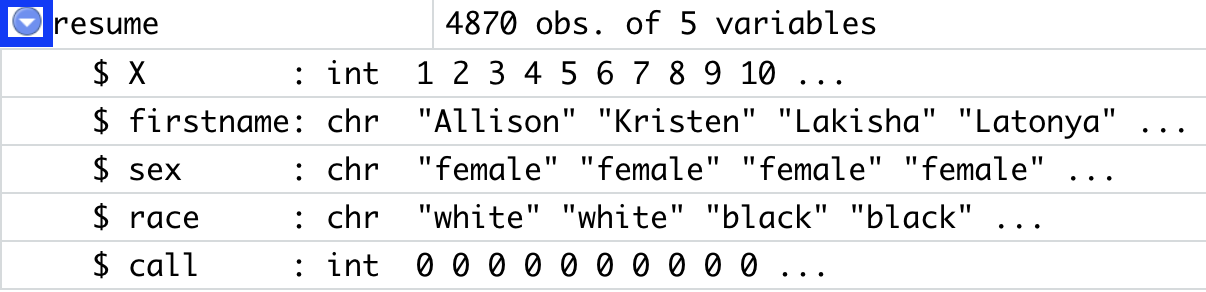
\includegraphics[width=0.9\linewidth]{images/06_bluearrow} 

}

\caption{Loading a Data Frame}\label{fig:bluearrow}
\end{figure}

If you click on the name of the data frame, RStudio will open up a spreadsheet of all the data. This is similar to how we would use the \texttt{browse} command when using Stata. This allows you to look through the raw data and understand what the various variables are and what values they may take.

There are also a few ways to summarize information about the data frame. For example \texttt{ncol()}, retrieves the number of columns. \texttt{nrow()} retrieves the number of rows In this example, there are 5 variables, so there will be 5 columns. There are 4,870 observations, so there are 4,870 rows. One thing we can do to quickly get a sense of the data is to type \texttt{summary(resume)}. This provides some simple summary statistics for each variable in the data frame.

\begin{Shaded}
\begin{Highlighting}[]
\FunctionTok{summary}\NormalTok{(resume)}
\end{Highlighting}
\end{Shaded}

\begin{verbatim}
       X         firstname             sex           
 Min.   :   1   Length:4870        Length:4870       
 1st Qu.:1218   Class :character   Class :character  
 Median :2436   Mode  :character   Mode  :character  
 Mean   :2436                                        
 3rd Qu.:3653                                        
 Max.   :4870                                        
     race                call        
 Length:4870        Min.   :0.00000  
 Class :character   1st Qu.:0.00000  
 Mode  :character   Median :0.00000  
                    Mean   :0.08049  
                    3rd Qu.:0.00000  
                    Max.   :1.00000  
\end{verbatim}

For numeric variables, this command provides the min, max, 25th percentile (called 1st Quartile), median, mean, 75th percentile (called 3rd Quantile) and max. For character variables, R just reports the length (i.e.~the number of observations). In this dataset, the variable \texttt{X} is just a variable that records the observation number, which goes from 1 to 4870. \texttt{firstname} is the name on the application. \texttt{sex} is either female or male. \texttt{race} is either white or Black. \texttt{call} is our main outcome of interest. It is equal to 1 if the fictitious application received a callback for an interview. It is equal to 0 if the fictitious application did not receive a callback.

Although we have already shown how to browse the raw data, it is sometimes inconvenient to look at the entire data frame, particularly when you have a very large dataset. However, it is often helpful to get a small snippet of the data. To do this, we can use the \texttt{head()} function. This shows you the first six observations in the data frame:

\begin{Shaded}
\begin{Highlighting}[]
\FunctionTok{head}\NormalTok{(resume)}
\end{Highlighting}
\end{Shaded}

\begin{verbatim}
  X firstname    sex  race call
1 1   Allison female white    0
2 2   Kristen female white    0
3 3   Lakisha female black    0
4 4   Latonya female black    0
5 5    Carrie female white    0
6 6       Jay   male white    0
\end{verbatim}

Similarly, we can use the \texttt{tail()} function to show the last six observations in the data frame.

Next, let's talk about a big distinction between R and Stata. In Stata, we always had one data set. This makes it easy to reference variables: we just type the variable name. For example, if we had wanted to take the mean of the variable \texttt{call} in Stata, we would have typed \texttt{sum\ call}.

In R, however, you can load multiple data frames at a time. This is actually a really nice feature of R, especially when you are trying to merge data frames together. What it means, however, is that whenever you reference a variable, you need to reference both the variable name, as well as the data frame that it comes from. For example, to reference the variable \texttt{call} within the data frame \texttt{resume}, we type \texttt{resume\$call}.

For example, if we wanted to look at the first six observations, but only for \texttt{call}, we would type:

\begin{Shaded}
\begin{Highlighting}[]
\FunctionTok{head}\NormalTok{(resume}\SpecialCharTok{$}\NormalTok{call)}
\end{Highlighting}
\end{Shaded}

\begin{verbatim}
[1] 0 0 0 0 0 0
\end{verbatim}

It is a very common mistake for beginners to forget to specify both the data frame and the variable. This can lead to some confusing errors, so always make sure that you are specifying both the data frame and the variable in R.

Now that we have our data loaded and we understand how to reference variables, let's begin to explore the data. First, let's get a sense of the callback rates for these fictitious applicants. Remember, our variable \texttt{call} is equal to 1 if the resume received a callback for an interview. Therefore, if we take the average of this variable, then this value will be equal to the fraction of individuals who received a callback. If you don't follow this logic, make sure to flip back to Chapter 1.5 to review why this is true.

We already know how to take the average of a vector, we use the \texttt{mean()} function. But a column in a data frame is just a vector. So we can use this function to find the callback rate:

\begin{Shaded}
\begin{Highlighting}[]
\FunctionTok{mean}\NormalTok{(resume}\SpecialCharTok{$}\NormalTok{call)}
\NormalTok{[}\DecValTok{1}\NormalTok{] }\FloatTok{0.08049281}
\end{Highlighting}
\end{Shaded}

So around 8 percent of all applicants received a callback for an interview. Low callback rates are pretty common in these settings. Next, let's look at our other main variable of interest. To get the distribution of race we can use the \texttt{table()} function, which prints out a table of frequencies:

\begin{Shaded}
\begin{Highlighting}[]
\FunctionTok{table}\NormalTok{(resume}\SpecialCharTok{$}\NormalTok{race)}

\NormalTok{black white }
 \DecValTok{2435}  \DecValTok{2435} 
\end{Highlighting}
\end{Shaded}

So there are equal numbers of white and Black applicants. This was by design. The researchers were particularly interested in understanding racial disparities in callback rates. Therefore, they designed the experiment to have equal rates of white and Black applicants.

Lastly, let's talk about how to save a data frame. In most empirical projects, we won't have such a clean data frame to start with. We may need to drop certain observations, clean certain variables, and overall, make many changes to our data. It is never a good idea to overwrite your raw data, so after you are done cleaning your data, you should save a new data file.

To save a csv file in R, you can use the \texttt{write.csv} function:

\begin{Shaded}
\begin{Highlighting}[]
\FunctionTok{write.csv}\NormalTok{(resume, }\AttributeTok{file=}\StringTok{"resume1.csv"}\NormalTok{)}
\end{Highlighting}
\end{Shaded}

This will save the data frame \texttt{resume} which is currently in memory as a csv file named \texttt{resume1.csv}. This file will be saved in your working directory.

There is also another format for data that is common in R: ``RData''. You can save your file as and RData file by using the \texttt{save()} function.

\begin{Shaded}
\begin{Highlighting}[]
\FunctionTok{save}\NormalTok{(resume, }\AttributeTok{file=}\StringTok{"resume1.RData"}\NormalTok{)}
\end{Highlighting}
\end{Shaded}

There is often not a strong argument between saving as a csv file verse an RData file. In general, however, csv files are often more portable across different statistical programs. Most of the data we will be using in the R section of the course will therefore be stored as csv files.

\section{Logic}\label{logic}

Just like in Stata, logical statements will be a key concept in this section of the course. To remind you, a logical statement is any statement that is either true or false. In R, there is a special type of object, called \textbf{logical objects}, which are objects that take on either the value \texttt{TRUE} or \texttt{FALSE}.

Sometimes we may want to subset our data to observations in which a certain statement is true. For example, maybe we have a dataset that has individuals from many states, but we only want to analyze data for California. In this case, we may want to subset to observations such that the logical statement ``Individual resides in California'' is true. We are often going to be using logical statements in R to manipulate our data.

So how do we create these objects that are either true or false? We use logical operators. We have seen many logical operators in the Stata portion of the class. For example, the double equals sign \texttt{==} is a logical operator that tests whether two things are equal. Here is a list of all the logical operators we will be using throughout the R portion of the course:

\begin{itemize}
\item
  \texttt{!} -- not
\item
  \texttt{\&} -- and
\item
  \texttt{\textbar{}} -- or
\item
  \texttt{==} -- equals
\item
  \texttt{!=} -- not equals
\item
  \texttt{\textgreater{}} -- greater than
\item
  \texttt{\textless{}} -- less than
\item
  \texttt{\textgreater{}=} -- greater than or equal to
\item
  \texttt{\textless{}=} -- less than or equal to
\end{itemize}

Now that we've written out the different logical operators, let's see how to use these in R. To begin, let's start with a simple logical statement: ``5 is equal to 6''. The way we type this in R is we type \texttt{5==6}. This statement is of course false, so if we type this into R it should yield \texttt{FALSE}.

\begin{Shaded}
\begin{Highlighting}[]
\DecValTok{5}\SpecialCharTok{==}\DecValTok{6}
\NormalTok{[}\DecValTok{1}\NormalTok{] }\ConstantTok{FALSE}
\end{Highlighting}
\end{Shaded}

If instead, our logical statement is ``5 is equal to 5'', then this statement should yield \texttt{TRUE}.

\begin{Shaded}
\begin{Highlighting}[]
\DecValTok{5}\SpecialCharTok{==}\DecValTok{5}
\NormalTok{[}\DecValTok{1}\NormalTok{] }\ConstantTok{TRUE}
\end{Highlighting}
\end{Shaded}

Now let's write out ``5 is not equal to 6'', by using the \texttt{!} operator.

\begin{Shaded}
\begin{Highlighting}[]
\DecValTok{5}\SpecialCharTok{!=}\DecValTok{6}
\NormalTok{[}\DecValTok{1}\NormalTok{] }\ConstantTok{TRUE}
\end{Highlighting}
\end{Shaded}

But ``6 not equal to 6'' is of course \texttt{FALSE}:

\begin{Shaded}
\begin{Highlighting}[]
\DecValTok{6}\SpecialCharTok{!=}\DecValTok{6}
\NormalTok{[}\DecValTok{1}\NormalTok{] }\ConstantTok{FALSE}
\end{Highlighting}
\end{Shaded}

Now let's try to understand the \texttt{\&} operator. We use the \texttt{\&} operator when we want to test if two statements are \textbf{both} true. For example, let's imagine we have an individual who is 18 and lives in California. Then the statement ``This individual is 18 and lives in California'' is true. The way we might type this in R is \texttt{age==18\ \&\ state=="CA"}. Now let's do an example in R. Imagine we want to retrieve the answer to ``5 is equal to 5 and 5 is equal to 6''. In R we would type \texttt{5==5\ \&\ 5==6}. This statement is false because 5 is not equal to 6. If one of the statements is false (\texttt{5==6}) then the whole statement is false (\texttt{5==5\ \&\ 5==6}).

\begin{Shaded}
\begin{Highlighting}[]
\DecValTok{5}\SpecialCharTok{==}\DecValTok{5} \SpecialCharTok{\&} \DecValTok{5}\SpecialCharTok{==}\DecValTok{6}
\NormalTok{[}\DecValTok{1}\NormalTok{] }\ConstantTok{FALSE}
\end{Highlighting}
\end{Shaded}

In contrast, the statement ``5 is equal to 5 and 5 is greater than 4'' is true because both of the statements individually are true.

\begin{Shaded}
\begin{Highlighting}[]
\DecValTok{5}\SpecialCharTok{==}\DecValTok{5} \SpecialCharTok{\&} \DecValTok{5}\SpecialCharTok{\textgreater{}}\DecValTok{4}
\NormalTok{[}\DecValTok{1}\NormalTok{] }\ConstantTok{TRUE}
\end{Highlighting}
\end{Shaded}

Now let's discuss or statements. For an or statement, we are instead testing whether either statement is true. For example, if our statement is ``5 is equal to 5 or 5 is equal to 6'', then this is true if either \texttt{5==5\ \textbar{}\ 5==6}.

\begin{Shaded}
\begin{Highlighting}[]
\DecValTok{5}\SpecialCharTok{==}\DecValTok{5} \SpecialCharTok{|} \DecValTok{5}\SpecialCharTok{==}\DecValTok{6}
\NormalTok{[}\DecValTok{1}\NormalTok{] }\ConstantTok{TRUE}
\end{Highlighting}
\end{Shaded}

So far we have only applied logic to numbers in R. However, we can also apply this to vectors in R. This will be particularly important when we turn to data. We will often want to apply logical statements to variables in our data.

As a simple example, let's create a vector of graduation dates that has four entries:

\begin{Shaded}
\begin{Highlighting}[]
\NormalTok{graduationdates }\OtherTok{\textless{}{-}} \FunctionTok{c}\NormalTok{(}\DecValTok{2010}\NormalTok{,}\DecValTok{2001}\NormalTok{,}\DecValTok{2019}\NormalTok{,}\DecValTok{2003}\NormalTok{)}
\end{Highlighting}
\end{Shaded}

We can apply logical statements to the entire vector as well. For example, imagine we want to know which graduation dates are after 2010. We can type:

\begin{Shaded}
\begin{Highlighting}[]
\NormalTok{graduationdates}\SpecialCharTok{\textgreater{}}\DecValTok{2010}
\NormalTok{[}\DecValTok{1}\NormalTok{] }\ConstantTok{FALSE} \ConstantTok{FALSE}  \ConstantTok{TRUE} \ConstantTok{FALSE}
\end{Highlighting}
\end{Shaded}

This outputs another vector of four entries. Each entry tells us whether the corresponding entry in our \texttt{graduationdates} vector is greater than 2010. For entries 1, 2, and 4, this statement is \texttt{FALSE}. For entry 3, this statement is \texttt{TRUE}.

Next, let's learn how to compare two vectors. For example, imagine we have the vector of birth years that are supposed to be for the same individuals as in the graduation data:

\begin{Shaded}
\begin{Highlighting}[]
\NormalTok{birthyears}\OtherTok{\textless{}{-}} \FunctionTok{c}\NormalTok{(}\DecValTok{2016}\NormalTok{, }\DecValTok{1980}\NormalTok{, }\DecValTok{1996}\NormalTok{, }\DecValTok{1990}\NormalTok{)}
\end{Highlighting}
\end{Shaded}

By looking at this vector, it is clear something went wrong for the first individual. The individual is reported as being born in 2016 but graduated in 2010. There must have been some sort of data entry error for this individual. While we can quickly identify this mistake in our small data, imagine we have thousands of individuals. It won't be possible to identify all of the errors by manually going through the data.

Instead, we can simply test whether there are \texttt{birthyears} in the data that are greater than \texttt{graduationdates}

\begin{Shaded}
\begin{Highlighting}[]
\NormalTok{birthyears }\SpecialCharTok{\textgreater{}}\NormalTok{ graduationdates}
\NormalTok{[}\DecValTok{1}\NormalTok{]  }\ConstantTok{TRUE} \ConstantTok{FALSE} \ConstantTok{FALSE} \ConstantTok{FALSE}
\end{Highlighting}
\end{Shaded}

For this logical statement, the first element of \texttt{birthyears} is compared to the first element of \texttt{graduationdates}. Since 2016 is greater than 2010, the first element of the resulting logical vector is \texttt{TRUE}. The second element of \texttt{birthyears} is compared to the second element of \texttt{graduationdates}. Since 1980 is less than 2001, this statement is \texttt{FALSE}.

So far, we have just observed the output of these logical statements (i.e.~the output is displayed in the console). But imagine we want to save the output because we are using it in future analyses. For example, imagine we want to drop observations in which the birth year is greater than the graduation date. Well, we can simply store the output in a new vector by assigning it a name:

\begin{Shaded}
\begin{Highlighting}[]
\NormalTok{problem }\OtherTok{\textless{}{-}}\NormalTok{ birthyears }\SpecialCharTok{\textgreater{}}\NormalTok{ graduationdates}
\end{Highlighting}
\end{Shaded}

Now we have a vector \texttt{problem} that has been added to our environment. If we check the class of this vector we will see that it is a logical vector.

\begin{Shaded}
\begin{Highlighting}[]
\FunctionTok{class}\NormalTok{(problem)}
\NormalTok{[}\DecValTok{1}\NormalTok{] }\StringTok{"logical"}
\end{Highlighting}
\end{Shaded}

Now, the way logic functions in R is that it can function as a numeric variable. Specifically, the value \texttt{TRUE} is equal to the number 1. The value \texttt{FALSE} is equal to the number 0. Therefore, we can treat logical statements in the same way we've treated binary indicator variables in the past. For example, imagine I would like to compute the fraction of individuals for which there is a problem in the data, which is defined as a birth year greater than a graduation year. All I have to do is take the average of the \texttt{problem} vector.

\begin{Shaded}
\begin{Highlighting}[]
\FunctionTok{mean}\NormalTok{(problem)}
\NormalTok{[}\DecValTok{1}\NormalTok{] }\FloatTok{0.25}
\end{Highlighting}
\end{Shaded}

Why does this get us the right result? Because the problem vector is equal to \texttt{TRUE\ FALSE\ FALSE\ FALSE}. R will interpret this vector as \texttt{1\ 0\ 0\ 0}. The mean value of this vector is therefore equal to 0.25. In other words, for 25 percent of individuals, there is a problem in the data. If you prefer to have the vector in numeric format instead of logical, you can also change it yourself by using the \texttt{as.numeric()} function:

\begin{Shaded}
\begin{Highlighting}[]
\FunctionTok{as.numeric}\NormalTok{(problem)}
\NormalTok{[}\DecValTok{1}\NormalTok{] }\DecValTok{1} \DecValTok{0} \DecValTok{0} \DecValTok{0}
\end{Highlighting}
\end{Shaded}

This just changes how the information is displayed to you in R, not the actual information itself.

\section{Subsetting Vectors}\label{subsetting-vectors}

Often we want to extract certain elements of a vector, which is known as \textbf{subsetting}. In R, to subset a vector we use \texttt{{[}{]}}. Inside the \texttt{{[}{]}} we can place a number to extract a certain element. For example, if we type \texttt{graduationdate{[}3{]}}, we would extract the third element of the vector \texttt{graduationdate}. This is referred to as \textbf{indexing}. In this example, 3 is the index number.

We can also use logic to extract certain elements. For example, in general, if we type \texttt{vec{[}logical\ statement{]}}, then only the elements for which the logical statement is true will be extracted. This will be especially useful when using data because it is common we want to extract elements that meet a certain condition, for example, individuals above the age of 18, or counties located in California, etc.

To understand how to subset vectors in R, let's run through a few examples. First, let's re-create our \texttt{graduationdates} vector.

\begin{Shaded}
\begin{Highlighting}[]
\NormalTok{graduationdates }\OtherTok{\textless{}{-}} \FunctionTok{c}\NormalTok{(}\DecValTok{2010}\NormalTok{,}\DecValTok{2001}\NormalTok{,}\DecValTok{2019}\NormalTok{,}\DecValTok{2003}\NormalTok{)}
\end{Highlighting}
\end{Shaded}

The third entry of \texttt{graduationdates} is 2019. If we want to extract this entry, we can just type

\begin{Shaded}
\begin{Highlighting}[]
\NormalTok{graduationdates[}\DecValTok{3}\NormalTok{]}
\NormalTok{[}\DecValTok{1}\NormalTok{] }\DecValTok{2019}
\end{Highlighting}
\end{Shaded}

Instead of extracting an element, you can also use what is referred to as negative indexing. If you put a negative in front of the index number, then you get all elements of the vector, except that element. For example, let's see what happens when we type \texttt{graduationdates{[}-3{]}}

\begin{Shaded}
\begin{Highlighting}[]
\NormalTok{graduationdates[}\SpecialCharTok{{-}}\DecValTok{3}\NormalTok{]}
\NormalTok{[}\DecValTok{1}\NormalTok{] }\DecValTok{2010} \DecValTok{2001} \DecValTok{2003}
\end{Highlighting}
\end{Shaded}

The output is another vector, but now only composed of three elements. The new vector has dropped the third element of \texttt{graduationdates}.

You can also use indexing to subset multiple elements of a vector. For example, imagine we would like to extract the first and third elements of the \texttt{graduationdates} vector. To do this, we create a vector of indices.

\begin{Shaded}
\begin{Highlighting}[]
\NormalTok{graduationdates[}\FunctionTok{c}\NormalTok{(}\DecValTok{1}\NormalTok{,}\DecValTok{3}\NormalTok{)]}
\NormalTok{[}\DecValTok{1}\NormalTok{] }\DecValTok{2010} \DecValTok{2019}
\end{Highlighting}
\end{Shaded}

If you recall, \texttt{c(1,3)} is a vector. The \texttt{c()} function concatenates 1 and 3 into a vector. The way R reads the statement above is ``extract from the vector \texttt{graduationdates}, the 1st and 3rd element.

Now that we understand how to subset vectors using numbers and vectors, let's learn how to index using logic. Instead of entering a vector of numbers as the index, we can directly enter a vector of \texttt{TRUE} and \texttt{FALSE}. Only the elements for which the entry is \texttt{TRUE} will be extracted. To see how this works, let's try to understand the example below:

\begin{Shaded}
\begin{Highlighting}[]
\NormalTok{graduationdates[}\FunctionTok{c}\NormalTok{(}\ConstantTok{TRUE}\NormalTok{, }\ConstantTok{FALSE}\NormalTok{, }\ConstantTok{TRUE}\NormalTok{, }\ConstantTok{FALSE}\NormalTok{)]}
\NormalTok{[}\DecValTok{1}\NormalTok{] }\DecValTok{2010} \DecValTok{2019}
\end{Highlighting}
\end{Shaded}

The vector \texttt{c(TRUE,\ FALSE,\ TRUE,\ FALSE)} is \texttt{TRUE} for the 1st and 3rd element. Therefore, only the first and third elements have been extracted. A more common way you might see this used is through another vector or variable. For example, imagine we also have a vector that contains the school that the student attended.

\begin{Shaded}
\begin{Highlighting}[]
\NormalTok{school }\OtherTok{\textless{}{-}} \FunctionTok{c}\NormalTok{(}\StringTok{"UCSD"}\NormalTok{, }\StringTok{"UCB"}\NormalTok{, }\StringTok{"UCLA"}\NormalTok{, }\StringTok{"UCR"}\NormalTok{)}
\end{Highlighting}
\end{Shaded}

Imagine we want to retrieve the graduation date for the student who attended UCSD. If we type \texttt{school=="UCSD"}, we will get a vector of 4 elements:

\begin{Shaded}
\begin{Highlighting}[]
\NormalTok{school}\SpecialCharTok{==}\StringTok{"UCSD"}
\NormalTok{[}\DecValTok{1}\NormalTok{]  }\ConstantTok{TRUE} \ConstantTok{FALSE} \ConstantTok{FALSE} \ConstantTok{FALSE}
\end{Highlighting}
\end{Shaded}

Only the first element is \texttt{TRUE}. Therefore, if we use this vector to subset the \texttt{graduationdate} vector, we will retrieve the graduation date of the student who attended UCSD.

\begin{Shaded}
\begin{Highlighting}[]
\NormalTok{graduationdates[school}\SpecialCharTok{==}\StringTok{"UCSD"}\NormalTok{]}
\NormalTok{[}\DecValTok{1}\NormalTok{] }\DecValTok{2010}
\end{Highlighting}
\end{Shaded}

Next, let's turn from our simple examples to our empirical application for this section: correspondence studies. First, let's re-load the data on fictitious applications from Bertrand and Mullainathan (2004).

\begin{Shaded}
\begin{Highlighting}[]
\NormalTok{resume }\OtherTok{\textless{}{-}} \FunctionTok{read.csv}\NormalTok{(}\StringTok{"resume.csv"}\NormalTok{)}
\end{Highlighting}
\end{Shaded}

Remember, we can really think of each variable in a dataframe as a vector. Therefore, we don't really need to learn anything new. We just need to apply what we have learned so far to this new data structure.

First, let's talk about how to use logical subsetting on a variable. What happens if we type \texttt{resume\$race=="black"}. Well, \texttt{resume\$race} is a vector with 4,870 elements. It takes on values ``white'' or ``black''. Therefore, \texttt{resume\$race=="black"} is also a vector with 4,870 elements. The first element is \texttt{TRUE} if the first individual in the dataset had a Black-sounding name. The first element is \texttt{FALSE} if the first element had a white-sounding name. You can convince yourself of this by typing:

\begin{Shaded}
\begin{Highlighting}[]
\NormalTok{vec }\OtherTok{\textless{}{-}}\NormalTok{ resume}\SpecialCharTok{$}\NormalTok{race}\SpecialCharTok{==}\StringTok{"black"}
\end{Highlighting}
\end{Shaded}

And then studying the resulting vector \texttt{vec}. What happens if we then add a function around this vector? For example, if we type \texttt{sum(resume\$race=="black")}, then R should add up all the values of the vector \texttt{resume\$race=="black"}. Recall, R interprets a value of \texttt{TRUE} as equal to 1, and a value of \texttt{FALSE} as equal to 0. So if we type \texttt{sum(resume\$race=="black")}, we will just retrieve the total number of applications with Black-sounding names.

\begin{Shaded}
\begin{Highlighting}[]
\FunctionTok{sum}\NormalTok{(resume}\SpecialCharTok{$}\NormalTok{race}\SpecialCharTok{==}\StringTok{"black"}\NormalTok{)}
\NormalTok{[}\DecValTok{1}\NormalTok{] }\DecValTok{2435}
\end{Highlighting}
\end{Shaded}

We can subset one variable using a logical statement built from another variable. For example, imagine we want to compute the callback rate for Black applicants. Therefore, we want to compute the average of \texttt{call} only for individuals such that \texttt{race=="black"}. In R, we can write out this statement as follows:

\begin{Shaded}
\begin{Highlighting}[]
\FunctionTok{mean}\NormalTok{(resume}\SpecialCharTok{$}\NormalTok{call[resume}\SpecialCharTok{$}\NormalTok{race}\SpecialCharTok{==}\StringTok{"black"}\NormalTok{])}
\NormalTok{[}\DecValTok{1}\NormalTok{] }\FloatTok{0.06447639}
\end{Highlighting}
\end{Shaded}

It is easiest to interpret this line of code by starting at the indexing step. \texttt{{[}resume\$race=="black"{]}} restricts to observations for which the applicant is Black. \texttt{resume\$call{[}resume\$race=="black"{]}} is the vector \texttt{call}, but only restricted to the observations for which the applicant is Black. Finally, by placing the entire block inside the \texttt{mean()} function, we are computing the average of \texttt{resume\$call} for applicants such that \texttt{resume\$race=="black"}. If we want to compare to white applicants, we can simply type:

\begin{Shaded}
\begin{Highlighting}[]
\FunctionTok{mean}\NormalTok{(resume}\SpecialCharTok{$}\NormalTok{call[resume}\SpecialCharTok{$}\NormalTok{race}\SpecialCharTok{==}\StringTok{"white"}\NormalTok{])}
\NormalTok{[}\DecValTok{1}\NormalTok{] }\FloatTok{0.09650924}
\end{Highlighting}
\end{Shaded}

\section{Subsetting Data Frames}\label{subsetting-data-frames}

Next, we will discuss how to subset data frames. To illustrate this concept, we are first going to generate a small data frame in R:

\begin{Shaded}
\begin{Highlighting}[]
\NormalTok{students }\OtherTok{\textless{}{-}} \FunctionTok{data.frame}\NormalTok{(}\AttributeTok{school=}\FunctionTok{c}\NormalTok{(}\StringTok{"UCSD"}\NormalTok{, }\StringTok{"UCB"}\NormalTok{, }\StringTok{"UCSD"}\NormalTok{),}
                       \AttributeTok{graduationdate=}\FunctionTok{c}\NormalTok{(}\DecValTok{2010}\NormalTok{, }\DecValTok{2019}\NormalTok{, }\DecValTok{2015}\NormalTok{))}
\end{Highlighting}
\end{Shaded}

To understand what the code above produced, let's look at the dataframe \texttt{student}:

\begin{Shaded}
\begin{Highlighting}[]
\NormalTok{students}
\NormalTok{  school graduationdate}
\DecValTok{1}\NormalTok{   UCSD           }\DecValTok{2010}
\DecValTok{2}\NormalTok{    UCB           }\DecValTok{2019}
\DecValTok{3}\NormalTok{   UCSD           }\DecValTok{2015}
\end{Highlighting}
\end{Shaded}

This data frame has two variables: \texttt{school} and \texttt{graduationdate}. The first column of the data frame corresponds to \texttt{school} and the second corresponds to \texttt{graduationdate}. The data frame has three total observations. To extract a specific value of the data frame, we can again use indexing. When using indexing with a vector, we could specify a single number, and that would pluck out that element. Now, with a data frame, we need to specify two numbers. First, we will specify the row we would like to extract and then we will specify the column. For example, to extract the value in the 3rd row, 1st column, we would type:

\begin{Shaded}
\begin{Highlighting}[]
\NormalTok{students[}\DecValTok{3}\NormalTok{,}\DecValTok{1}\NormalTok{]}
\NormalTok{[}\DecValTok{1}\NormalTok{] }\StringTok{"UCSD"}
\end{Highlighting}
\end{Shaded}

It outputs ``UCSD'' because the the third student in the data frame went to UCSD and the 1st column in the data frame corresponds to the variable \texttt{school}.

Instead of extracting specific elements of a data frame, you can also extract entire columns and rows. For example, to extract the first-row type:

\begin{Shaded}
\begin{Highlighting}[]
\NormalTok{students[}\DecValTok{1}\NormalTok{,]}
\NormalTok{  school graduationdate}
\DecValTok{1}\NormalTok{   UCSD           }\DecValTok{2010}
\end{Highlighting}
\end{Shaded}

The second entry in the \texttt{{[},{]}} always corresponds to the column. Since it is blank, R extracted all columns for the first observation. Similarly, you can extract a single column by leaving the rows portion of the index blank. For example, to extract the second column, type:

\begin{Shaded}
\begin{Highlighting}[]
\NormalTok{students[,}\DecValTok{2}\NormalTok{]}
\NormalTok{[}\DecValTok{1}\NormalTok{] }\DecValTok{2010} \DecValTok{2019} \DecValTok{2015}
\end{Highlighting}
\end{Shaded}

Now, since the row index is blank, R extracts values from all rows, but just the second column.
You can also use a vector to specify what observations or columns you would like to retrieve. For example, imagine we think there was an error with recording the graduation date for the second observation in our data frame. To be careful, we would like to drop this individual from the data frame. In other words, we want to extract rows 1 and 3 of the data frame and leave out row 2. To do this, we can subset by specifying a vector of indices. The vector will contain the indices of every row we want in the final data frame:

\begin{Shaded}
\begin{Highlighting}[]
\NormalTok{students[}\FunctionTok{c}\NormalTok{(}\DecValTok{1}\NormalTok{,}\DecValTok{3}\NormalTok{),]}
\NormalTok{  school graduationdate}
\DecValTok{1}\NormalTok{   UCSD           }\DecValTok{2010}
\DecValTok{3}\NormalTok{   UCSD           }\DecValTok{2015}
\end{Highlighting}
\end{Shaded}

We can do the same thing with negative indexing, as seen below:

\begin{Shaded}
\begin{Highlighting}[]
\NormalTok{students[}\SpecialCharTok{{-}}\DecValTok{2}\NormalTok{,]}
\NormalTok{  school graduationdate}
\DecValTok{1}\NormalTok{   UCSD           }\DecValTok{2010}
\DecValTok{3}\NormalTok{   UCSD           }\DecValTok{2015}
\end{Highlighting}
\end{Shaded}

Next, let's discuss how to use logic to subset data frames. For example, imagine we want to extract all individuals that went to UCSD. In other words, we only want individuals such that \texttt{students\$school=="UCSD"} is TRUE. Remember, if we type this into R we will get a vector of TRUE and FALSE statements:

\begin{Shaded}
\begin{Highlighting}[]
\NormalTok{students}\SpecialCharTok{$}\NormalTok{school}\SpecialCharTok{==}\StringTok{"UCSD"}
\NormalTok{[}\DecValTok{1}\NormalTok{]  }\ConstantTok{TRUE} \ConstantTok{FALSE}  \ConstantTok{TRUE}
\end{Highlighting}
\end{Shaded}

Then, just like with vectors, if we use this logical statement to subset, we will only retrieve observations such that the statement is TRUE. In this case, this statement is TRUE for the first and third observations:

\begin{Shaded}
\begin{Highlighting}[]
\NormalTok{students[students}\SpecialCharTok{$}\NormalTok{school}\SpecialCharTok{==}\StringTok{"UCSD"}\NormalTok{,]}
\NormalTok{  school graduationdate}
\DecValTok{1}\NormalTok{   UCSD           }\DecValTok{2010}
\DecValTok{3}\NormalTok{   UCSD           }\DecValTok{2015}
\end{Highlighting}
\end{Shaded}

Indexing data frames and vectors in this way is a useful skill that will be portable to other software programs that you may encounter in the future. However, in R, there are often easier solutions to subsetting data. For example, the function \texttt{subset} is often used to subset data frames. When we learn about the \texttt{tidyverse} in a future chapter, there will be a function that is again useful for subsetting.

The general syntax for the subset command is:

\begin{Shaded}
\begin{Highlighting}[]
\FunctionTok{subset}\NormalTok{(df, logical statement)}
\end{Highlighting}
\end{Shaded}

The resulting data frame will be a subset of the data frame named \texttt{df} restricted only to the observations for which the logical statement after the comma is TRUE. For example, to create a data frame of UCSD students, we could type:

\begin{Shaded}
\begin{Highlighting}[]
\FunctionTok{subset}\NormalTok{(students,students}\SpecialCharTok{$}\NormalTok{school}\SpecialCharTok{==}\StringTok{"UCSD"}\NormalTok{)}
\NormalTok{  school graduationdate}
\DecValTok{1}\NormalTok{   UCSD           }\DecValTok{2010}
\DecValTok{3}\NormalTok{   UCSD           }\DecValTok{2015}
\end{Highlighting}
\end{Shaded}

Remember, to save this data frame as a new object in R, you will need to assign it a name.

\begin{Shaded}
\begin{Highlighting}[]
\NormalTok{ucsd\_students }\OtherTok{\textless{}{-}} \FunctionTok{subset}\NormalTok{(students,students}\SpecialCharTok{$}\NormalTok{school}\SpecialCharTok{==}\StringTok{"UCSD"}\NormalTok{)}
\end{Highlighting}
\end{Shaded}

\section{Conclusion}\label{conclusion-4}

Now, let's put everything that we've learned in this chapter together to study discrimination in hiring practices. To get started, let's load in the resume data.

\begin{Shaded}
\begin{Highlighting}[]
\NormalTok{resume }\OtherTok{\textless{}{-}} \FunctionTok{read.csv}\NormalTok{(}\StringTok{"resume.csv"}\NormalTok{)}
\end{Highlighting}
\end{Shaded}

When we are exploring a new data frame, it is often helpful to get a sense of the variables and the values they take. Let's look at the first few observations in the data in order to remind ourselves what is in the data:

\begin{Shaded}
\begin{Highlighting}[]
\FunctionTok{head}\NormalTok{(resume)}
\NormalTok{  X firstname    sex  race call}
\DecValTok{1} \DecValTok{1}\NormalTok{   Allison female white    }\DecValTok{0}
\DecValTok{2} \DecValTok{2}\NormalTok{   Kristen female white    }\DecValTok{0}
\DecValTok{3} \DecValTok{3}\NormalTok{   Lakisha female black    }\DecValTok{0}
\DecValTok{4} \DecValTok{4}\NormalTok{   Latonya female black    }\DecValTok{0}
\DecValTok{5} \DecValTok{5}\NormalTok{    Carrie female white    }\DecValTok{0}
\DecValTok{6} \DecValTok{6}\NormalTok{       Jay   male white    }\DecValTok{0}
\end{Highlighting}
\end{Shaded}

Our main outcome of interest is whether an individual received a callback for an interview. In the data frame, a 0 represents the resume did not get a callback. A 1 represents the resume did get a callback. Because the data is stored in this way, we can simply take the average of the variable call in order to retrieve the overall callback rate:

\begin{Shaded}
\begin{Highlighting}[]
\FunctionTok{mean}\NormalTok{(resume}\SpecialCharTok{$}\NormalTok{call)}
\NormalTok{[}\DecValTok{1}\NormalTok{] }\FloatTok{0.08049281}
\end{Highlighting}
\end{Shaded}

Remember, whenever we specify a variable, we need to specify both the data frame as well as the variable name. As we will see later, it is often helpful to have multiple data frames loaded into memory in R.

In this experiment, we want to understand whether the callback rate varies by race. Before proceeding, let's look at the distribution of race across applications:

\begin{Shaded}
\begin{Highlighting}[]
\FunctionTok{table}\NormalTok{(resume}\SpecialCharTok{$}\NormalTok{race)}

\NormalTok{black white }
 \DecValTok{2435}  \DecValTok{2435} 
\end{Highlighting}
\end{Shaded}

There are 2435 resumes with white-sounding names and 2435 resumes with Black-sounding names. Remember, these are fictitious resumes, and the experimenters designed the study so that there would be an equal number of applications for white and Black applicants.

Note that we could retrieve the same information using logic. When we type a logical statement, R will return a logical object that is composed of \texttt{TRUE} and \texttt{FALSE}. Whenever R sees \texttt{TRUE} it interprets a 1, and whenever R sees \texttt{FALSE} it interprets a 0. For example, if we type:

\begin{Shaded}
\begin{Highlighting}[]
\FunctionTok{sum}\NormalTok{(resume}\SpecialCharTok{$}\NormalTok{race}\SpecialCharTok{==}\StringTok{"black"}\NormalTok{)}
\NormalTok{[}\DecValTok{1}\NormalTok{] }\DecValTok{2435}
\end{Highlighting}
\end{Shaded}

We get a value of 2435. Why? Well, \texttt{resume\$race=="black} is a vector of length 4870. Half of the elements are \texttt{TRUE} while the other half are \texttt{FALSE}. The \texttt{sum()} function adds up all the values of a vector. All the \texttt{TRUE} values are equal to 1 and all of the \texttt{FALSE} values are equal to zero. Therefore, it is simply counting up all the applications for which the statement is \texttt{TRUE}.

Now, let's get to the main analysis, which studies whether callback rates vary by race. To do so, let's first find the callback rate for applicants with Black-sounding names. To do this, we will again utilize logic:

\begin{Shaded}
\begin{Highlighting}[]
\FunctionTok{mean}\NormalTok{(resume}\SpecialCharTok{$}\NormalTok{call[resume}\SpecialCharTok{$}\NormalTok{race}\SpecialCharTok{==}\StringTok{"black"}\NormalTok{])}
\NormalTok{[}\DecValTok{1}\NormalTok{] }\FloatTok{0.06447639}
\end{Highlighting}
\end{Shaded}

Here we are using indexing. \texttt{{[}resume\$race=="black"{]}} subsets to Black applicants. Because we have put this inside \texttt{mean(resume\$call{[}{]})}, then R will retrieve the average of the \texttt{resume\$call} vector, but restrict to Black applicants. As we can see, about 6.4 percent of Black applicants receive a callback.

Let's now compare this to white applicants:

\begin{Shaded}
\begin{Highlighting}[]
\FunctionTok{mean}\NormalTok{(resume}\SpecialCharTok{$}\NormalTok{call[resume}\SpecialCharTok{$}\NormalTok{race}\SpecialCharTok{==}\StringTok{"white"}\NormalTok{])}
\NormalTok{[}\DecValTok{1}\NormalTok{] }\FloatTok{0.09650924}
\end{Highlighting}
\end{Shaded}

Before interpreting these findings, it is helpful to point out that there are a couple of different ways we could have performed the analysis. For example, sometimes it is helpful to generate different data frames for subsets of your data. We could have done this through indexing or through the \texttt{subset} function:

For example, to create a data frame restricted to Black applicants we could type:

\begin{Shaded}
\begin{Highlighting}[]
\NormalTok{resume\_blacknames }\OtherTok{\textless{}{-}}\NormalTok{ resume[resume}\SpecialCharTok{$}\NormalTok{race}\SpecialCharTok{==}\StringTok{"black"}\NormalTok{,]}
\NormalTok{resume\_whitenames }\OtherTok{\textless{}{-}}\NormalTok{ resume[resume}\SpecialCharTok{$}\NormalTok{race}\SpecialCharTok{==}\StringTok{"white"}\NormalTok{,]}
\end{Highlighting}
\end{Shaded}

Then, to calculate the callback rate for Black applicants, we should just reference this data frame:

\begin{Shaded}
\begin{Highlighting}[]
\FunctionTok{mean}\NormalTok{(resume\_blacknames}\SpecialCharTok{$}\NormalTok{call)}
\NormalTok{[}\DecValTok{1}\NormalTok{] }\FloatTok{0.06447639}
\FunctionTok{mean}\NormalTok{(resume\_whitenames}\SpecialCharTok{$}\NormalTok{call)}
\NormalTok{[}\DecValTok{1}\NormalTok{] }\FloatTok{0.09650924}
\end{Highlighting}
\end{Shaded}

Now that we have performed the main analysis, let's summarize our findings. Around 9.7 percent of white applicants receive a callback, while only 6.4 percent of Black applicants receive a callback. Therefore, there is a 3.3 percentage point disparity in callback rates. This is a substantial disparity. The baseline callback rates are quite low in this setting. A 3.3 percentage point disparity implies white applicants are more than 50 percent more likely to receive a callback relative to Black applicants:

\[
\text{Percent Increase in Callbacks for White Apps}=\frac{9.7-6.4}{6.4}=0.516
\]
This highlights a stark disparity in labor-market outcomes. Given the empirical design: randomizing race across applications, these disparities cannot be driven by other factors that employers take into account when making hiring decisions. They are due to the names associated with the applications, and how those names proxy for race.

This empirical design has become widely popular. It has been used to study discrimination across other demographics, for example, gender, sexual orientation, and disability status. It has also increased in scope, with recent experiments sending out thousands and thousands of fictitious resumes in order to understand discrimination at some of the largest employers in the U.S (see Kline, Rose, and Walters 2022).\citep{kline2021systemic}

\section*{Function Descriptions}\label{function-descriptions}
\addcontentsline{toc}{section}{Function Descriptions}

\textbf{Setup Functions}

\begin{itemize}
\item
  \texttt{getwd()} --- retrieves the current working directory
\item
  \texttt{setwd("pathname")} -- sets the working directory to whatever is contained in pathname. For example, if I type \texttt{setwd("Users/davidarnold/Desktop")}, then my working directory will be set to my desktop.
\item
  \texttt{\textless{}-} -- this is called the assignment operator. It assigns some value to an object. This can be used to create numeric objects, character objects, vectors, as well as dataframes.
\item
  \texttt{read.csv(csvfile.csv)} -- reads in a csv file into R. To save the csv file as a dataframe, assign it a name. \texttt{df\ \textless{}-\ read.csv("csvfile.csv")}
\end{itemize}

\textbf{Data Exploration Commands}

\begin{itemize}
\item
  \texttt{nrow()} -- retrieves number of rows in a data frame.
\item
  \texttt{ncol()} -- retrieves number of columns in a dataframe
\item
  \texttt{summary(dataframe)} - lists all variables in the dataframe. For numeric variables, computes some key quantiles.
\item
  \texttt{names(dataframe)} - retrieves names of all columns in the dataframe
\item
  \texttt{mean(dataframe\$varname)} -- retrives the mean value of \texttt{varname} which is a variable inside the data frame \texttt{dataframe}.
\item
  \texttt{table(dataframe\$varname)} -- retrieves a table of frequencies for the variable \texttt{varname} within the data frame \texttt{dataframe}. This can be used for string variables as well as categorical variables.
\end{itemize}

\chapter{The Rug Rat Race}\label{the-rug-rat-race}

\section{Time Diaries}\label{time-diaries}

Figure \ref{fig:rugrat} plots a somewhat puzzling finding from Ramey and Ramey (2010). The figure shows the amount of hours per week mothers spend on childcare over time. For both college-educated and less-than-college-educated mothers, time spent on childcare rose dramatically in the early 1990s.

\begin{figure}

{\centering 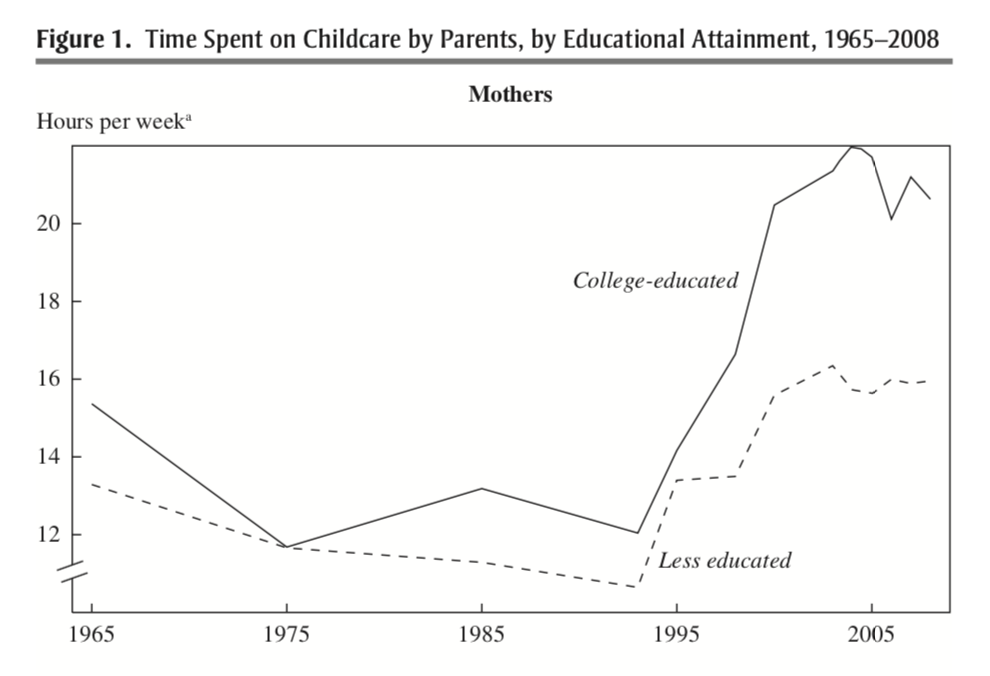
\includegraphics[width=0.9\linewidth]{images/07_RugRatMothers} 

}

\caption{Time Spent on Childcare by Parents, by Educational Attainment, 1965-2008}\label{fig:rugrat}
\end{figure}

This rise occurs for both college-educated and less-educated mothers, but the rise is especially dramatic for college-educated mothers. Why is this puzzling? Well, this is a time period in which the returns to education were increasing a lot. In other words, these college-educated mothers had a lot to gain from working in the labor market, but in the data, we find they are spending more time on childcare. In this section of the course, we will explore why.

In order to explore this question we will use data from the American Time Use Survey (ATUS). This is a survey administered by the Bureau of Labor Statistics, an agency that collects many important statistics concerning the U.S. economy.

The data is based on ``time diaries'' which are detailed descriptions of the activities in a given day. For example, if the interview was held on a Tuesday, the individual would report everything they did on Monday (from 4 AM Monday to 4 AM Tuesday). This is a useful survey technique to get an accurate representation of how much time people spend on various activities.

Before digging into the data, however, we are going to learn a bit more about the R programming language. In particular, in this chapter we will cover some important functions for \textbf{data wrangling}.

\section{Conditional Statements}\label{conditional-statements}

The basic idea behind conditional statements is that sometimes in R we want to execute some code, but only if a certain condition is true. Conditional statements are incredibly important in all programming languages. For example, when you type something on a computer and get an error statement, that is a conditional statement at work. A certain condition was met (some error in this case), so the computer output an error message.

The way we will implement this idea in R is to use \texttt{if} statements. The general syntax for \texttt{if} statements is:

\begin{Shaded}
\begin{Highlighting}[]
\ControlFlowTok{if}\NormalTok{ (logical statement) \{}
  
\NormalTok{  code to be executed }\ControlFlowTok{if}\NormalTok{ logical statement is }\ConstantTok{TRUE}
  
\NormalTok{\}}
\end{Highlighting}
\end{Shaded}

It might be a bit easier to understand this syntax with a simple example. To begin, we are going to create an object in R called \texttt{door} which is equal to \texttt{locked}.

\begin{Shaded}
\begin{Highlighting}[]
\NormalTok{door }\OtherTok{\textless{}{-}} \StringTok{"locked"}
\end{Highlighting}
\end{Shaded}

Now, we are going to write some code to return a message if the object \texttt{door} is indeed locked.

\begin{Shaded}
\begin{Highlighting}[]
\ControlFlowTok{if}\NormalTok{ (door}\SpecialCharTok{==}\StringTok{"locked"}\NormalTok{) \{}
  
  \FunctionTok{print}\NormalTok{(}\StringTok{"sorry, you need a key to enter"}\NormalTok{)}
  
\NormalTok{\}}
\NormalTok{[}\DecValTok{1}\NormalTok{] }\StringTok{"sorry, you need a key to enter"}
\end{Highlighting}
\end{Shaded}

What is R doing here? Well, because we have assigned the value \texttt{locked} to the object door, the logical statement in parentheses \texttt{door=="locked"} is TRUE. Therefore, if we run this section of code, the code inside the curly brackets \texttt{\{\}} will be executed. In this case, the code just prints a message.

What happens if we change the value of door to \texttt{unlocked}. Well, in that case \texttt{door=="locked"} is no longer TRUE. Therefore, the code inside the brackets will \textbf{not} be executed.

\begin{Shaded}
\begin{Highlighting}[]
\NormalTok{door }\OtherTok{\textless{}{-}} \StringTok{"unlocked"}

\ControlFlowTok{if}\NormalTok{ (door}\SpecialCharTok{==}\StringTok{"locked"}\NormalTok{) \{}
  
  \FunctionTok{print}\NormalTok{(}\StringTok{"sorry, you need a key to enter"}\NormalTok{)}
  
\NormalTok{\}}
\end{Highlighting}
\end{Shaded}

Let's try another example. Say we take a random draw from three numbers: -1, 0, and 1. We can take a random draw from this list of numbers by using the sample function:

\begin{Shaded}
\begin{Highlighting}[]
\NormalTok{x }\OtherTok{\textless{}{-}} \FunctionTok{sample}\NormalTok{(}\SpecialCharTok{{-}}\DecValTok{1}\SpecialCharTok{:}\DecValTok{1}\NormalTok{,}\DecValTok{1}\NormalTok{)}
\NormalTok{x}
\NormalTok{[}\DecValTok{1}\NormalTok{] }\DecValTok{1}
\end{Highlighting}
\end{Shaded}

The part of the code \texttt{-1:1} controls what numbers will be drawn. If you type \texttt{-1:1} in R, you will see it prints out the numbers -1,0, and 1. The second part of the code \texttt{,1} tells R how many random samples to take. In this case, just 1. So overall, this code is simply setting x equal to either -1, 0, or 1 and doing so randomly.

So now let's write a conditional statement that depends on the outcome of x. Let's write some code that returns the absolute value of x, but only if x is less than zero.

\begin{Shaded}
\begin{Highlighting}[]
\ControlFlowTok{if}\NormalTok{ (x}\SpecialCharTok{\textless{}}\DecValTok{0}\NormalTok{)\{}
  \FunctionTok{abs}\NormalTok{(x)}
\NormalTok{\}}
\end{Highlighting}
\end{Shaded}

Next, let's discuss \texttt{else} statements. Sometimes, we want to execute certain code if the statement is TRUE, but some other code if it is FALSE. For example, in our first example, imagine if the \texttt{door} object is not equal to \texttt{locked} then we want R to print out the message \texttt{Please\ Come\ in!}. The way we can do this in R is with an \texttt{else} statement:

\begin{Shaded}
\begin{Highlighting}[]
\NormalTok{door }\OtherTok{\textless{}{-}} \StringTok{"locked"}
\ControlFlowTok{if}\NormalTok{ (door}\SpecialCharTok{==}\StringTok{"locked"}\NormalTok{)\{}
  \FunctionTok{print}\NormalTok{(}\StringTok{"Sorry, you need a key to enter"}\NormalTok{)}
\NormalTok{\} }\ControlFlowTok{else}\NormalTok{ \{}
  \FunctionTok{print}\NormalTok{(}\StringTok{"Please Come in!"}\NormalTok{)}
\NormalTok{\}}
\NormalTok{[}\DecValTok{1}\NormalTok{] }\StringTok{"Sorry, you need a key to enter"}
\end{Highlighting}
\end{Shaded}

Since we set \texttt{door\textless{}-"locked"}, the first statement \texttt{door=="locked"} is TRUE. Therefore, the code inside the first curly brackets was executed. Now, let's change door to unlocked and see how this changes the output.

\begin{Shaded}
\begin{Highlighting}[]
\NormalTok{door }\OtherTok{\textless{}{-}} \StringTok{"unlocked"}
\ControlFlowTok{if}\NormalTok{ (door}\SpecialCharTok{==}\StringTok{"locked"}\NormalTok{)\{}
  \FunctionTok{print}\NormalTok{(}\StringTok{"Sorry, you need a key to enter"}\NormalTok{)}
\NormalTok{\} }\ControlFlowTok{else}\NormalTok{ \{}
  \FunctionTok{print}\NormalTok{(}\StringTok{"Please Come in!"}\NormalTok{)}
\NormalTok{\}}
\NormalTok{[}\DecValTok{1}\NormalTok{] }\StringTok{"Please Come in!"}
\end{Highlighting}
\end{Shaded}

So now the first statement \texttt{door=="locked"} is FALSE. Therefore, R executes the code after the \texttt{else\ \{\}}.

There are a few important notes about conditional statements before we move on. First, the \texttt{else} must appear on the same line as the end curly bracket \texttt{\}}. If it doesn't, then R doesn't know what logical statement to connect the \texttt{else} to. Second, R will execute the code after the \texttt{else} brackets if \texttt{door=="locked"} is FALSE for any reason.

For example, imagine I set \texttt{door\ \textless{}-\ "Locked"}. While it might look like the first logical statement \texttt{door=="locked"} is true, R is case sensitive. Therefore, in this case, the statement \texttt{door=="locked"} is FALSE. This implies that R will print out the words \texttt{Please\ Come\ in!}.

\section{For Loops}\label{for-loops}

In data analysis, we often find ourselves performing the same operation many times. We might be performing the same analysis for different variables or performing the same calculation for many different numbers.

One way to perform this analysis is through writing scripts with many, many lines of code. Much of the code might be exactly the same, but simply changes a single number or variable. An alternative way to perform this computation is through \textbf{loops}. Although we are learning how to implement loops in R, loops are a concept that you should be aware of in any programming language.

The general form for a loop in R is given below:

\begin{Shaded}
\begin{Highlighting}[]
\ControlFlowTok{for}\NormalTok{ (some set of things) \{}
\NormalTok{  do some stuff}
\NormalTok{\}}
\end{Highlighting}
\end{Shaded}

The \texttt{for} tells R this will be a for loop. Some set of things will depend on exactly what you are trying to do. Often, it will be a list of numbers. The next part of the code \texttt{\{} tells R that everything that follows is part of the loop. The end curly bracket \texttt{\}} tells R that the loop is over.

To understand these concepts more concretely. We are going to go through a simple example. Let's imagine that someone has demanded you use R to print out \texttt{2*i} for \texttt{i} equal to 1, 2, 3, 4, and 5. In simpler language, multiply each number between 1 and 5 by 2 and then print out the result. We are going to perform this in what we will call the brute force method.

First, let's print out \texttt{2*1}

\begin{Shaded}
\begin{Highlighting}[]
\NormalTok{i }\OtherTok{\textless{}{-}}\DecValTok{1}
\FunctionTok{print}\NormalTok{(}\DecValTok{2}\SpecialCharTok{*}\NormalTok{i)}
\NormalTok{[}\DecValTok{1}\NormalTok{] }\DecValTok{2}
\end{Highlighting}
\end{Shaded}

So why did we code this in such a roundabout way? Why not directly type \texttt{2*1}. Well, once we go through the loop it will become clear why we are coding this in a somewhat roundabout way. What you need to understand now is exactly what the code is doing. First, it is creating an object named \texttt{i} that is equal to \texttt{1}. Then, it is multiplying that object by 2 and printing out the result. Now, we have to do this for the number 2.

\begin{Shaded}
\begin{Highlighting}[]
\NormalTok{i }\OtherTok{\textless{}{-}} \DecValTok{2} 
\FunctionTok{print}\NormalTok{(}\DecValTok{2}\SpecialCharTok{*}\NormalTok{i)}
\NormalTok{[}\DecValTok{1}\NormalTok{] }\DecValTok{4}
\end{Highlighting}
\end{Shaded}

Note that the second part of the code \texttt{print(2*i)} is exactly the same as before. That will be key when we are writing our loop. We can continue to do this for the rest of the numbers

\begin{Shaded}
\begin{Highlighting}[]
\NormalTok{i }\OtherTok{\textless{}{-}} \DecValTok{3} 
\FunctionTok{print}\NormalTok{(}\DecValTok{2}\SpecialCharTok{*}\NormalTok{i)}
\NormalTok{[}\DecValTok{1}\NormalTok{] }\DecValTok{6}
\end{Highlighting}
\end{Shaded}

\begin{Shaded}
\begin{Highlighting}[]
\NormalTok{i }\OtherTok{\textless{}{-}} \DecValTok{4} 
\FunctionTok{print}\NormalTok{(}\DecValTok{2}\SpecialCharTok{*}\NormalTok{i)}
\NormalTok{[}\DecValTok{1}\NormalTok{] }\DecValTok{8}
\end{Highlighting}
\end{Shaded}

\begin{Shaded}
\begin{Highlighting}[]
\NormalTok{i }\OtherTok{\textless{}{-}} \DecValTok{5} 
\FunctionTok{print}\NormalTok{(}\DecValTok{2}\SpecialCharTok{*}\NormalTok{i)}
\NormalTok{[}\DecValTok{1}\NormalTok{] }\DecValTok{10}
\end{Highlighting}
\end{Shaded}

In each block of code, the only thing changing is what \texttt{i} is equal to. Well, this is exactly what a loop does.

\begin{Shaded}
\begin{Highlighting}[]
\ControlFlowTok{for}\NormalTok{ (i }\ControlFlowTok{in} \DecValTok{1}\SpecialCharTok{:}\DecValTok{5}\NormalTok{)\{}
  
  \FunctionTok{print}\NormalTok{(}\DecValTok{2}\SpecialCharTok{*}\NormalTok{i)}

\NormalTok{\}}
\NormalTok{[}\DecValTok{1}\NormalTok{] }\DecValTok{2}
\NormalTok{[}\DecValTok{1}\NormalTok{] }\DecValTok{4}
\NormalTok{[}\DecValTok{1}\NormalTok{] }\DecValTok{6}
\NormalTok{[}\DecValTok{1}\NormalTok{] }\DecValTok{8}
\NormalTok{[}\DecValTok{1}\NormalTok{] }\DecValTok{10}
\end{Highlighting}
\end{Shaded}

When we type \texttt{for\ (i\ in\ 1:5)} we are telling R to execute \texttt{print(2*i)} 5 times. The first time, \texttt{i==1}. This is referred to as the first \textbf{iteration} of the loop. Once it has executed the code for \texttt{i==1}, it should move on to \texttt{i==2}. This is the second iteration of the loop.

The great thing about this is that it can greatly increase the efficiency of our coding. For example, imagine we wanted to print out \texttt{2*i} for \texttt{i=1:100}. If we go the brute force way, that would be 200 lines of code (first setting \texttt{i} equal to the given number and then executing the code). But with the loop, only one thing changes: in the first line we simply type \texttt{for\ (i\ in\ 1:100)}.

In this example we are \textbf{iterating} over a list of numbers from 1 to 5. You can also iterate over other objects in R. For example, instead of iterating over a sequence of numbers, you can iterate over a vector.

\begin{Shaded}
\begin{Highlighting}[]
\ControlFlowTok{for}\NormalTok{ (i }\ControlFlowTok{in} \FunctionTok{c}\NormalTok{(}\DecValTok{3}\NormalTok{,}\DecValTok{10}\NormalTok{,}\DecValTok{99}\NormalTok{))\{}
  \FunctionTok{print}\NormalTok{(}\DecValTok{2}\SpecialCharTok{*}\NormalTok{i)}
\NormalTok{\}}
\NormalTok{[}\DecValTok{1}\NormalTok{] }\DecValTok{6}
\NormalTok{[}\DecValTok{1}\NormalTok{] }\DecValTok{20}
\NormalTok{[}\DecValTok{1}\NormalTok{] }\DecValTok{198}
\end{Highlighting}
\end{Shaded}

In this loop, in the first iteration, \texttt{i} is equal to 3. In the second iteration \texttt{i} is equal to 10. In the third \texttt{i} is equal to 99.

Next, we are going to go through an example that loops over words instead of numbers. In this example, we are going to print out a to do list. Let's say we need to do three sets of homework assignments: math, reading, and writing. To start this example, let's create a vector of the assignments we need to do:

\begin{Shaded}
\begin{Highlighting}[]
\NormalTok{homework }\OtherTok{\textless{}{-}} \FunctionTok{c}\NormalTok{(}\StringTok{"math"}\NormalTok{, }\StringTok{"reading"}\NormalTok{, }\StringTok{"writing"}\NormalTok{)}
\end{Highlighting}
\end{Shaded}

We can loop over the contents of this vector in order to print out a to-do list.

\begin{Shaded}
\begin{Highlighting}[]
\ControlFlowTok{for}\NormalTok{ (i }\ControlFlowTok{in}\NormalTok{ homework) \{}
  \FunctionTok{cat}\NormalTok{(}\StringTok{"Do"}\NormalTok{, i, }\StringTok{"}\SpecialCharTok{\textbackslash{}n}\StringTok{"}\NormalTok{)}
\NormalTok{\}}
\NormalTok{Do math }
\NormalTok{Do reading }
\NormalTok{Do writing }
\end{Highlighting}
\end{Shaded}

We introduced a few new things here, so let's go through the code slowly. First, instead of looping over numbers here, we are looping over words. In the first iteration \texttt{i} is equal to the first entry of the vector \texttt{homework}. Therefore, \texttt{i} is equal to \texttt{math} in the first iteration.

Next, we have used a knew function \texttt{cat()}. This function concatenates and prints. Therefore, if we type \texttt{cat("Do",i)} what you should interpret (in the first) iteration is that we are forming the sentence \texttt{Do\ Math}. The last part \texttt{,"\textbackslash{}n"} is telling R to display the next text a line down. When you want to skip a line in a word document, you just press Enter. In R, you can type \texttt{"\textbackslash{}n"}. If you are still unsure what \texttt{"\textbackslash{}n"} is doing, you should try to take it out of the code and see how the result looks.

In this example, we are looping over the words in \texttt{homework}. An alternative way to write this loop out will take advantage of indexing. The following code performs the exact same process as above, it is just coded in a slightly different way.

\begin{Shaded}
\begin{Highlighting}[]
\ControlFlowTok{for}\NormalTok{ (i }\ControlFlowTok{in} \DecValTok{1}\SpecialCharTok{:}\FunctionTok{length}\NormalTok{(homework)) \{}
  \FunctionTok{cat}\NormalTok{(}\StringTok{"Do"}\NormalTok{, homework[i], }\StringTok{"}\SpecialCharTok{\textbackslash{}n}\StringTok{"}\NormalTok{)}
\NormalTok{\}}
\NormalTok{Do math }
\NormalTok{Do reading }
\NormalTok{Do writing }
\end{Highlighting}
\end{Shaded}

In this loop, we are again looping over numbers. \texttt{length(homework)} is equal to 3. So we are looping over the numbers 1 to 3. In the first iteration, we are concatenating the words ``Do'' and \texttt{homework{[}1{]}}. Since \texttt{homework{[}1{]}} is equal to Math, we are retrieving the exact same output as before.

So why would we want to code this loop in this way? Well, in this setting, it doesn't really matter how you write the code. However, that won't always be the case. Using the loop index (\texttt{i}) in order to subset vectors or data frames is a very common practice, so it is important to be exposed to this aspect of loops as well.

\section{For Loops (Data)}\label{for-loops-data}

Next, we are going to use for loops to make calculations in our data. To remind you, our empirical application is going to study how time spent on childcare, particularly for mothers, has changed over time. To begin, we are going to load in data from the American Time Use Survey.

\begin{Shaded}
\begin{Highlighting}[]
\NormalTok{rr }\OtherTok{\textless{}{-}} \FunctionTok{read.csv}\NormalTok{(}\StringTok{"rugratrace.csv"}\NormalTok{)}
\FunctionTok{dim}\NormalTok{(rr)}
\NormalTok{[}\DecValTok{1}\NormalTok{] }\DecValTok{106020}     \DecValTok{54}
\end{Highlighting}
\end{Shaded}

As you can see, this is a pretty large dataset. There are 106,020 observations and 54 variables. Because this data is so large, we are first going to explain a subset of variables that we will be focusing on. Our goal is to compute time spent on childcare over time for mothers. The variable \texttt{mother2} is an indicator variable that is equal to one if the individual is a mother with a child currently living in the household. \texttt{age} is holds the age of the individual. \texttt{childtot} is the total hours spent on childcare in a week. \texttt{dataset} actually holds the year the data was collected. Different years come from datasets. This will be important to keep in mind going forward with the analysis.

Our goal is to follow the Ramey and Ramey (2010) analysis as closely as possible. In order to do this, we are going to make a number of restrictions in our data so that we have the same sample of individuals studied by Ramey and Ramey (2010). This will involve restricting to mothers between ages 25 and 34 with a child in the household. In terms of the variables in the data frame, these are individuals such that \texttt{age\textgreater{}=25\ \&\ age\textless{}=34\ \&\ mother2==1}. This is a logical statement composed of three statements, strung together by \texttt{\&} operators. Therefore, in order to be \texttt{TRUE}, every individual statement must be \texttt{TRUE}. You should be able to convince yourself that this statement is only \texttt{TRUE} for mothers between the ages of 25-34.

The way we can subset to these individuals is through the \texttt{subset} command.

\begin{Shaded}
\begin{Highlighting}[]
\NormalTok{mothers2534 }\OtherTok{\textless{}{-}} \FunctionTok{subset}\NormalTok{(rr, mother2}\SpecialCharTok{==}\DecValTok{1} \SpecialCharTok{\&}\NormalTok{ age}\SpecialCharTok{\textgreater{}=}\DecValTok{25} \SpecialCharTok{\&}\NormalTok{ age}\SpecialCharTok{\textless{}=}\DecValTok{34}\NormalTok{)}
\end{Highlighting}
\end{Shaded}

Now we have a data frame restricted to the sample we are analyzing. Our goal is to compute the average amount of \texttt{childtot} over years (in our case, over different values of the variable \texttt{dataset}). Therefore, what we need next is a list of the years in the data frame.

Luckily, there is a function \texttt{unique()} that will come in handy here. \texttt{unique()} retrieves list of the unique values of a variable. In other words, if we type \texttt{unique(rr\$dataset)} we will get a list of all the years in the data frame.

\begin{Shaded}
\begin{Highlighting}[]
\NormalTok{years }\OtherTok{\textless{}{-}} \FunctionTok{unique}\NormalTok{(mothers2534}\SpecialCharTok{$}\NormalTok{dataset)}
\NormalTok{years}
\NormalTok{ [}\DecValTok{1}\NormalTok{] }\DecValTok{1965} \DecValTok{1975} \DecValTok{1985} \DecValTok{1993} \DecValTok{1998} \DecValTok{2003} \DecValTok{2004} \DecValTok{2005} \DecValTok{2006} \DecValTok{2007} \DecValTok{2008}
\end{Highlighting}
\end{Shaded}

So we are going to write a loop and iterate over the years. Before writing the full loop, let's make sure we understand how to code this for the first iteration. First, let's set \texttt{i} equal to one.

\begin{Shaded}
\begin{Highlighting}[]
\NormalTok{i }\OtherTok{\textless{}{-}} \DecValTok{1} 
\end{Highlighting}
\end{Shaded}

Next, let's subset the data so that we create a dataframe that only contains observations such that \texttt{dataset==years{[}i{]}}. Since \texttt{i} is currently equal to 1, this will subset the data to observations from 1965.

\begin{Shaded}
\begin{Highlighting}[]
\NormalTok{sub }\OtherTok{\textless{}{-}} \FunctionTok{subset}\NormalTok{(mothers2534, dataset}\SpecialCharTok{==}\NormalTok{years[i])}
\end{Highlighting}
\end{Shaded}

Since the data frame \texttt{sub} only contains observations from 1965, we can simply take the average of \texttt{childtot} within this data frame to retrieve the average amount of hours spent on childcare per week in 1965.

\begin{Shaded}
\begin{Highlighting}[]
\FunctionTok{mean}\NormalTok{(sub}\SpecialCharTok{$}\NormalTok{childtot)}
\NormalTok{[}\DecValTok{1}\NormalTok{] }\FloatTok{13.82249}
\end{Highlighting}
\end{Shaded}

When we actually go to iterating over a loop, we will want to keep track of what each number printed out corresponds to. Therefore, let's use the \texttt{cat()} function to clarify exactly what is being printed out. We are actually going to print out two things. First, we are going to print out the year we are studying. Then, we are going to print out the average childcare in that year.

\begin{Shaded}
\begin{Highlighting}[]
\CommentTok{\# prints out year}
\FunctionTok{cat}\NormalTok{(}\StringTok{"Year"}\NormalTok{, years[i],}\StringTok{"}\SpecialCharTok{\textbackslash{}n}\StringTok{"}\NormalTok{)}
\NormalTok{Year }\DecValTok{1965} 
\CommentTok{\# prints out average childcare for this group}
\FunctionTok{cat}\NormalTok{(}\StringTok{"Average childcare per week:"}\NormalTok{, }\FunctionTok{mean}\NormalTok{(sub}\SpecialCharTok{$}\NormalTok{childtot),}\StringTok{"}\SpecialCharTok{\textbackslash{}n}\StringTok{"}\NormalTok{)}
\NormalTok{Average childcare per week}\SpecialCharTok{:} \FloatTok{13.82249} 
\end{Highlighting}
\end{Shaded}

Now that we have written all the code for \texttt{i\textless{}-1}, we just need to put this code inside a loop that loops over from 1 to the total number of years. The total number of years is given by \texttt{length(years)}:

\begin{Shaded}
\begin{Highlighting}[]
\ControlFlowTok{for}\NormalTok{ (i }\ControlFlowTok{in} \DecValTok{1}\SpecialCharTok{:}\FunctionTok{length}\NormalTok{(years)) \{}
  
  \CommentTok{\# subset to year i}
\NormalTok{  sub }\OtherTok{\textless{}{-}} \FunctionTok{subset}\NormalTok{(mothers2534, dataset}\SpecialCharTok{==}\NormalTok{years[i])}

  \CommentTok{\# prints out year}
  \FunctionTok{cat}\NormalTok{(}\StringTok{"Year"}\NormalTok{, years[i],}\StringTok{"}\SpecialCharTok{\textbackslash{}n}\StringTok{"}\NormalTok{)}
  
  \CommentTok{\# prints out average childcare for this group}
  \FunctionTok{cat}\NormalTok{(}\StringTok{"Average childcare per week:"}\NormalTok{, }\FunctionTok{mean}\NormalTok{(sub}\SpecialCharTok{$}\NormalTok{childtot),}\StringTok{"}\SpecialCharTok{\textbackslash{}n}\StringTok{"}\NormalTok{)}
  
\NormalTok{\}}
\end{Highlighting}
\end{Shaded}

\begin{verbatim}
Year 1965 
Average childcare per week: 13.82249 
Year 1975 
Average childcare per week: 9.758393 
Year 1985 
Average childcare per week: 12.86947 
Year 1993 
Average childcare per week: 9.244037 
Year 1998 
Average childcare per week: 14.83095 
Year 2003 
Average childcare per week: 16.02707 
Year 2004 
Average childcare per week: 16.45709 
Year 2005 
Average childcare per week: 15.68486 
Year 2006 
Average childcare per week: 16.23848 
Year 2007 
Average childcare per week: 17.01327 
Year 2008 
Average childcare per week: 16.24845 
\end{verbatim}

As we can see in this table, this replicates one of the main findings in Ramey and Ramey (2010). In 1965-1993, the average time spent on childcare fluctuated between 9 and 13 hours. From 1998 onwards, the average amount of time spent on childcare increases dramatically, often between 15-17 hours per week on average.

\section{Tidyverse}\label{tidyverse}

So far we have been using what is referred to as base R. We have only utilized functions that come standard in R. However, one of the main strengths of R is its very active user community. Because R is open-source, users can write their own packages in R and make them widely available. This means the functionality of R is essentially growing every day.

One of the most useful collection of packages for data analysis is the tidyverse package. This collection of packages can do many things. We will cover a small portion of what the package is capable of. If you want to get a more thorough understanding of the tidyverse, you can go to \href{https://r4ds.had.co.nz/}{R for Data Science} and read more.

But before using the tidyverse, we actually have to install it into our version of R. In order to install a package, you can use the \texttt{install.packages()} function. For example, to install tidyverse, type:

\begin{Shaded}
\begin{Highlighting}[]
\FunctionTok{install.packages}\NormalTok{(}\StringTok{"tidyverse"}\NormalTok{)}
\end{Highlighting}
\end{Shaded}

This will download all the necessary components of the tidyverse package onto your computer. You only need to install a package once.

Next, in order to use a package in a given R session, you need to load it into memory using the \texttt{library()} function:

\begin{Shaded}
\begin{Highlighting}[]
\FunctionTok{library}\NormalTok{(tidyverse)}
\end{Highlighting}
\end{Shaded}

A common mistake for students is to forget to load a package for a given R session. If you do this, you might get an error such as ``{[}function{]} not found''. If you are using functions from an external package, you need to make sure to load that package in every session of R that you want to use it in.

The first concept we will learn from tidyverse is the concept of a tibble. A tibble is very similar to what we have been calling a data frame. For our purposes, you can think of a tibble as synonymous with data frame. The main difference is in how the data is stored and presented. For us, this won't matter too much. For larger datasets, sometimes loading as a tibble can make a big difference in terms of how long computations take.

To start, let's load \texttt{rugratrace.csv} as a data frame.

\begin{Shaded}
\begin{Highlighting}[]
\NormalTok{rr }\OtherTok{\textless{}{-}} \FunctionTok{read.csv}\NormalTok{(}\StringTok{"rugratrace.csv"}\NormalTok{)}
\end{Highlighting}
\end{Shaded}

To convert a data frame to a tibble, you can use the function \texttt{as\_tibble()}.

\begin{Shaded}
\begin{Highlighting}[]
\NormalTok{rr }\OtherTok{\textless{}{-}} \FunctionTok{as\_tibble}\NormalTok{(rr)}
\end{Highlighting}
\end{Shaded}

If you are following along, you may think the code above did not actually do anything. However, you can tell the difference if you print out the data set.

\begin{Shaded}
\begin{Highlighting}[]
\NormalTok{rr}
\CommentTok{\# A tibble: 106,020 x 54}
\NormalTok{   state   age   sex ethnic under18 under5 ageyngst student}
   \SpecialCharTok{\textless{}}\NormalTok{int}\SpecialCharTok{\textgreater{}} \ErrorTok{\textless{}}\NormalTok{int}\SpecialCharTok{\textgreater{}} \ErrorTok{\textless{}}\NormalTok{int}\SpecialCharTok{\textgreater{}}  \ErrorTok{\textless{}}\NormalTok{int}\SpecialCharTok{\textgreater{}}   \ErrorTok{\textless{}}\NormalTok{int}\SpecialCharTok{\textgreater{}}  \ErrorTok{\textless{}}\NormalTok{int}\SpecialCharTok{\textgreater{}}    \ErrorTok{\textless{}}\NormalTok{int}\SpecialCharTok{\textgreater{}}   \ErrorTok{\textless{}}\NormalTok{int}\SpecialCharTok{\textgreater{}}
 \DecValTok{1}    \DecValTok{23}    \DecValTok{26}     \DecValTok{2}     \SpecialCharTok{{-}}\DecValTok{9}       \DecValTok{4}      \DecValTok{2}       \ConstantTok{NA}       \DecValTok{0}
 \DecValTok{2}    \DecValTok{23}    \DecValTok{53}     \DecValTok{2}     \SpecialCharTok{{-}}\DecValTok{9}       \DecValTok{1}      \DecValTok{0}       \ConstantTok{NA}       \DecValTok{0}
 \DecValTok{3}    \DecValTok{23}    \DecValTok{21}     \DecValTok{2}     \SpecialCharTok{{-}}\DecValTok{9}       \DecValTok{2}      \DecValTok{2}       \ConstantTok{NA}       \DecValTok{0}
 \DecValTok{4}    \DecValTok{23}    \DecValTok{24}     \DecValTok{2}     \SpecialCharTok{{-}}\DecValTok{9}       \DecValTok{2}      \DecValTok{2}       \ConstantTok{NA}       \DecValTok{0}
 \DecValTok{5}    \DecValTok{23}    \DecValTok{25}     \DecValTok{2}     \SpecialCharTok{{-}}\DecValTok{9}       \DecValTok{3}      \DecValTok{1}       \ConstantTok{NA}       \DecValTok{0}
 \DecValTok{6}    \DecValTok{23}    \DecValTok{33}     \DecValTok{2}     \SpecialCharTok{{-}}\DecValTok{9}       \DecValTok{4}      \DecValTok{2}       \ConstantTok{NA}       \DecValTok{0}
 \DecValTok{7}    \DecValTok{23}    \DecValTok{26}     \DecValTok{2}     \SpecialCharTok{{-}}\DecValTok{9}       \DecValTok{3}      \DecValTok{2}       \ConstantTok{NA}       \DecValTok{0}
 \DecValTok{8}    \DecValTok{23}    \DecValTok{61}     \DecValTok{1}     \SpecialCharTok{{-}}\DecValTok{9}       \DecValTok{0}      \DecValTok{0}       \ConstantTok{NA}       \DecValTok{0}
 \DecValTok{9}    \DecValTok{23}    \DecValTok{57}     \DecValTok{1}     \SpecialCharTok{{-}}\DecValTok{9}       \DecValTok{0}      \DecValTok{0}       \ConstantTok{NA}       \DecValTok{0}
\DecValTok{10}    \DecValTok{23}    \DecValTok{43}     \DecValTok{2}     \SpecialCharTok{{-}}\DecValTok{9}       \DecValTok{2}      \DecValTok{1}       \ConstantTok{NA}       \DecValTok{0}
\CommentTok{\# i 106,010 more rows}
\CommentTok{\# i 46 more variables: act20 \textless{}int\textgreater{}, act21 \textless{}int\textgreater{},}
\CommentTok{\#   act26 \textless{}int\textgreater{}, act24 \textless{}int\textgreater{}, act22 \textless{}int\textgreater{}, act23 \textless{}int\textgreater{},}
\CommentTok{\#   act27 \textless{}int\textgreater{}, act67 \textless{}int\textgreater{}, act25 \textless{}int\textgreater{}, act29 \textless{}int\textgreater{},}
\CommentTok{\#   recwght \textless{}dbl\textgreater{}, dataset \textless{}int\textgreater{}, fips \textless{}int\textgreater{},}
\CommentTok{\#   married \textless{}int\textgreater{}, working \textless{}int\textgreater{}, fulltime \textless{}int\textgreater{},}
\CommentTok{\#   parttime \textless{}int\textgreater{}, mother2 \textless{}int\textgreater{}, father2 \textless{}int\textgreater{}, ...}
\end{Highlighting}
\end{Shaded}

You get more information printing out a tibble relative to a data frame. For our purposes, it won't matter too much if you load a dataset as a tibble or a data frame. However, it is important to understand these concepts, as you may see various online resources reference a tibble or a data frame. Generally, in this class we will load our datasets as tibbles from now on.

To load a dataset as a tibble directly, you can use the \texttt{read\_csv} function, the only difference being now an underscore separates the words in the function, rather than a period.

\begin{Shaded}
\begin{Highlighting}[]
\NormalTok{rr }\OtherTok{\textless{}{-}} \FunctionTok{read\_csv}\NormalTok{(}\StringTok{"rugratrace.csv"}\NormalTok{)}
\end{Highlighting}
\end{Shaded}

So now let's discuss some functions that come with tidyverse. The first functions we will introduce are \texttt{filter}, \texttt{select}, and \texttt{arrange}.

The \texttt{filter()} function retrieves observations (rows) in the data that meet a certain condition. For example, maybe you want to restrict the analysis to a certain demographic. You can use the \texttt{filter()} function to do this. In our example, we want to restrict to mothers between ages 25 and 34. We can use \texttt{filter()} to accomplish this. The general syntax for \texttt{filter()} is:

\begin{Shaded}
\begin{Highlighting}[]
\FunctionTok{filter}\NormalTok{(dataframe, some logical statement)}
\end{Highlighting}
\end{Shaded}

In our example, we can create the subset of the dataset we want by typing:

\begin{Shaded}
\begin{Highlighting}[]
\NormalTok{mothers2534 }\OtherTok{\textless{}{-}} \FunctionTok{filter}\NormalTok{(rr, age}\SpecialCharTok{\textless{}=}\DecValTok{34} \SpecialCharTok{\&}\NormalTok{ age}\SpecialCharTok{\textgreater{}=}\DecValTok{25} \SpecialCharTok{\&}\NormalTok{ mother2}\SpecialCharTok{==}\DecValTok{1}\NormalTok{)}
\end{Highlighting}
\end{Shaded}

You can use other logical operators in combination with filter as well. For example, imagine for a subset of our analysis we only want years between 2003 and 2008. We can use the operator \texttt{\%in\%} to accomplish this.

\begin{Shaded}
\begin{Highlighting}[]
\FunctionTok{filter}\NormalTok{(mothers2534, dataset}\SpecialCharTok{\%in\%}\DecValTok{2003}\SpecialCharTok{:}\DecValTok{2008}\NormalTok{)}
\CommentTok{\# A tibble: 6,416 x 54}
\NormalTok{   state   age   sex ethnic under18 under5 ageyngst student}
   \SpecialCharTok{\textless{}}\NormalTok{int}\SpecialCharTok{\textgreater{}} \ErrorTok{\textless{}}\NormalTok{int}\SpecialCharTok{\textgreater{}} \ErrorTok{\textless{}}\NormalTok{int}\SpecialCharTok{\textgreater{}}  \ErrorTok{\textless{}}\NormalTok{int}\SpecialCharTok{\textgreater{}}   \ErrorTok{\textless{}}\NormalTok{int}\SpecialCharTok{\textgreater{}}  \ErrorTok{\textless{}}\NormalTok{int}\SpecialCharTok{\textgreater{}}    \ErrorTok{\textless{}}\NormalTok{int}\SpecialCharTok{\textgreater{}}   \ErrorTok{\textless{}}\NormalTok{int}\SpecialCharTok{\textgreater{}}
 \DecValTok{1}    \ConstantTok{NA}    \DecValTok{32}     \DecValTok{2}     \ConstantTok{NA}       \DecValTok{1}     \ConstantTok{NA}        \DecValTok{2}       \DecValTok{1}
 \DecValTok{2}    \ConstantTok{NA}    \DecValTok{33}     \DecValTok{2}     \ConstantTok{NA}       \DecValTok{3}     \ConstantTok{NA}        \DecValTok{3}       \DecValTok{0}
 \DecValTok{3}    \ConstantTok{NA}    \DecValTok{33}     \DecValTok{2}     \ConstantTok{NA}       \DecValTok{1}     \ConstantTok{NA}        \DecValTok{7}       \DecValTok{0}
 \DecValTok{4}    \ConstantTok{NA}    \DecValTok{32}     \DecValTok{2}     \ConstantTok{NA}       \DecValTok{1}     \ConstantTok{NA}        \DecValTok{2}       \DecValTok{0}
 \DecValTok{5}    \ConstantTok{NA}    \DecValTok{25}     \DecValTok{2}     \ConstantTok{NA}       \DecValTok{1}     \ConstantTok{NA}        \DecValTok{6}       \DecValTok{0}
 \DecValTok{6}    \ConstantTok{NA}    \DecValTok{34}     \DecValTok{2}     \ConstantTok{NA}       \DecValTok{2}     \ConstantTok{NA}        \DecValTok{2}       \DecValTok{0}
 \DecValTok{7}    \ConstantTok{NA}    \DecValTok{31}     \DecValTok{2}     \ConstantTok{NA}       \DecValTok{1}     \ConstantTok{NA}        \DecValTok{2}       \DecValTok{0}
 \DecValTok{8}    \ConstantTok{NA}    \DecValTok{32}     \DecValTok{2}     \ConstantTok{NA}       \DecValTok{2}     \ConstantTok{NA}        \DecValTok{6}       \DecValTok{0}
 \DecValTok{9}    \ConstantTok{NA}    \DecValTok{32}     \DecValTok{2}     \ConstantTok{NA}       \DecValTok{2}     \ConstantTok{NA}       \DecValTok{12}       \DecValTok{0}
\DecValTok{10}    \ConstantTok{NA}    \DecValTok{32}     \DecValTok{2}     \ConstantTok{NA}       \DecValTok{2}     \ConstantTok{NA}        \DecValTok{3}       \DecValTok{0}
\CommentTok{\# i 6,406 more rows}
\CommentTok{\# i 46 more variables: act20 \textless{}int\textgreater{}, act21 \textless{}int\textgreater{},}
\CommentTok{\#   act26 \textless{}int\textgreater{}, act24 \textless{}int\textgreater{}, act22 \textless{}int\textgreater{}, act23 \textless{}int\textgreater{},}
\CommentTok{\#   act27 \textless{}int\textgreater{}, act67 \textless{}int\textgreater{}, act25 \textless{}int\textgreater{}, act29 \textless{}int\textgreater{},}
\CommentTok{\#   recwght \textless{}dbl\textgreater{}, dataset \textless{}int\textgreater{}, fips \textless{}int\textgreater{},}
\CommentTok{\#   married \textless{}int\textgreater{}, working \textless{}int\textgreater{}, fulltime \textless{}int\textgreater{},}
\CommentTok{\#   parttime \textless{}int\textgreater{}, mother2 \textless{}int\textgreater{}, father2 \textless{}int\textgreater{}, ...}
\end{Highlighting}
\end{Shaded}

This code is saying restrict to \texttt{mothers2534} only for observations such that dataset is in the range of 2003 through 2008. One important note here is that in the code above we did not overwrite \texttt{mothers2534}. That is why we can see the tibble being printed out. If you want to save the result of the \texttt{filter()} you need to assign the resulting tibble a name. Otherwise it will simply be printed to the console but not actually saved.

Next, let's discuss \texttt{select()}. This function chooses which variables you want to remain in your tibble. For example, in our current tibble we have many variables, but we really only need a subset of them for our analysis. So we can select the variables we really need:

\begin{Shaded}
\begin{Highlighting}[]
\NormalTok{mothers2534 }\OtherTok{\textless{}{-}} \FunctionTok{select}\NormalTok{(mothers2534, dataset, mother2, age, childtot)}
\end{Highlighting}
\end{Shaded}

Now if we print out \texttt{mothers2534}, it has only four variables now.

\begin{Shaded}
\begin{Highlighting}[]
\NormalTok{mothers2534}
\CommentTok{\# A tibble: 8,115 x 4}
\NormalTok{   dataset mother2   age childtot}
     \SpecialCharTok{\textless{}}\NormalTok{int}\SpecialCharTok{\textgreater{}}   \ErrorTok{\textless{}}\NormalTok{int}\SpecialCharTok{\textgreater{}} \ErrorTok{\textless{}}\NormalTok{int}\SpecialCharTok{\textgreater{}}    \ErrorTok{\textless{}}\NormalTok{dbl}\SpecialCharTok{\textgreater{}}
 \DecValTok{1}    \DecValTok{1965}       \DecValTok{1}    \DecValTok{26}     \DecValTok{7}   
 \DecValTok{2}    \DecValTok{1965}       \DecValTok{1}    \DecValTok{25}     \FloatTok{7.58}
 \DecValTok{3}    \DecValTok{1965}       \DecValTok{1}    \DecValTok{33}    \FloatTok{27.2} 
 \DecValTok{4}    \DecValTok{1965}       \DecValTok{1}    \DecValTok{26}     \FloatTok{4.20}
 \DecValTok{5}    \DecValTok{1965}       \DecValTok{1}    \DecValTok{25}     \FloatTok{6.42}
 \DecValTok{6}    \DecValTok{1965}       \DecValTok{1}    \DecValTok{26}    \FloatTok{14.8} 
 \DecValTok{7}    \DecValTok{1965}       \DecValTok{1}    \DecValTok{30}    \FloatTok{19.2} 
 \DecValTok{8}    \DecValTok{1965}       \DecValTok{1}    \DecValTok{33}     \FloatTok{8.75}
 \DecValTok{9}    \DecValTok{1965}       \DecValTok{1}    \DecValTok{30}    \FloatTok{16.3} 
\DecValTok{10}    \DecValTok{1965}       \DecValTok{1}    \DecValTok{29}    \FloatTok{29.8} 
\CommentTok{\# i 8,105 more rows}
\end{Highlighting}
\end{Shaded}

Finally, our last function for this section is \texttt{arrange()}. The \texttt{arrange()} function will sort the data based on the values of a variable. For example, imagine I want the observations in \texttt{mothers2534} to be arranged from the youngest age to the oldest age. I could type:

\begin{Shaded}
\begin{Highlighting}[]
\NormalTok{mothers2534 }\OtherTok{\textless{}{-}} \FunctionTok{arrange}\NormalTok{(mothers2534,age)}
\end{Highlighting}
\end{Shaded}

Now, we can verify that the youngest individuals are first:

\begin{Shaded}
\begin{Highlighting}[]
\FunctionTok{head}\NormalTok{(mothers2534}\SpecialCharTok{$}\NormalTok{age)}
\NormalTok{[}\DecValTok{1}\NormalTok{] }\DecValTok{25} \DecValTok{25} \DecValTok{25} \DecValTok{25} \DecValTok{25} \DecValTok{25}
\end{Highlighting}
\end{Shaded}

And the oldest are last.

\begin{Shaded}
\begin{Highlighting}[]
\FunctionTok{tail}\NormalTok{(mothers2534}\SpecialCharTok{$}\NormalTok{age)}
\NormalTok{[}\DecValTok{1}\NormalTok{] }\DecValTok{34} \DecValTok{34} \DecValTok{34} \DecValTok{34} \DecValTok{34} \DecValTok{34}
\end{Highlighting}
\end{Shaded}

If you instead want to sort from the oldest to youngest, you can use the function \texttt{desc()}, which stands for descending. In other words, the dataset will be sorted from the highest value to the lowest value.

\begin{Shaded}
\begin{Highlighting}[]
\NormalTok{mothers2534 }\OtherTok{\textless{}{-}} \FunctionTok{arrange}\NormalTok{(mothers2534,}\FunctionTok{desc}\NormalTok{(age))}
\FunctionTok{head}\NormalTok{(mothers2534}\SpecialCharTok{$}\NormalTok{age)}
\NormalTok{[}\DecValTok{1}\NormalTok{] }\DecValTok{34} \DecValTok{34} \DecValTok{34} \DecValTok{34} \DecValTok{34} \DecValTok{34}
\end{Highlighting}
\end{Shaded}

To finish off this chapter, let's summarize all of the new functions in tidyverse that we learned. First, \texttt{read\_csv()} is used in order to read data sets into R as a tibble. Next, we learned three functions that are useful for manipulating data. First, \texttt{filter()} selects observations of the tibble that meet a certain condition. In our case, mothers between the ages 25 and 34. Second, \texttt{select()} chooses which variables to keep in a tibble. In our case, we kept variables that indicated whether an individual is a mother, the year the data was collected, the age of the individual, and the amount of time spent on childcare of the individual. Lastly, \texttt{arrange()} is used to sort the data based on a value of a variable. In this chapter we showed how to use this to sort the data from youngest to oldest.

\section{The Pipe Operator}\label{the-pipe-operator}

In this section we are going to be going over the pipe operator: \texttt{\%\textgreater{}\%}. The pipe operator is a very useful tool to use when working with the tidyverse. For our purposes, we can use it to string along a number of commands. Eventually, we will see that this greatly improves the efficiency of our code. First, however, we simply need to learn mechanically what the pipe operator does (although why we are using it might not be immediately clear).

So far, in R, we have been applying functions to objects. For example, imagine we have a vector \texttt{x} and we want to take the mean. We would apply the \texttt{mean()} function to \texttt{x} by typing \texttt{mean(x)}. The pipe operator gives us an alternative way to write this. We can type: \texttt{x\ \%\textgreater{}\%\ mean()}. In general, when we have a function \texttt{f()}, we can either write \texttt{f(x)} or \texttt{x\ \%\textgreater{}\%\ f()}.

So what is the benefit of the pipe operator? Well, often in data analysis, we will want to apply many functions. For example, we may want to restrict to certain observations, select certain variables, and so on. We can think of this as applying many functions to an object in sequence. For example, if we first apply \texttt{f()}, then \texttt{g()} and then \texttt{h()} we can represent this as:

\begin{Shaded}
\begin{Highlighting}[]
\FunctionTok{h}\NormalTok{(}\FunctionTok{g}\NormalTok{(}\FunctionTok{f}\NormalTok{(x)))}
\end{Highlighting}
\end{Shaded}

Using pipe operators, we can equivalently write this out as:

\begin{Shaded}
\begin{Highlighting}[]
\NormalTok{x }\SpecialCharTok{\%\textgreater{}\%} 
\NormalTok{  f }\SpecialCharTok{\%\textgreater{}\%}
\NormalTok{    g }\SpecialCharTok{\%\textgreater{}\%}
\NormalTok{      h}
\end{Highlighting}
\end{Shaded}

What are we doing here? We are taking in an object x, and then applying f, and then applying g, and then applying h. When you read a pipe operator, you can think to yourself \textbf{and then}. This will be a helpful tool to remember what a pipe operator is doing. It is stringing together a number of different functions in R.

So far, this has been a relatively abstract discussion of pipe operators. Let's load some real data so we can see how this works in practice.

\begin{Shaded}
\begin{Highlighting}[]
\NormalTok{rr }\OtherTok{\textless{}{-}} \FunctionTok{read\_csv}\NormalTok{(}\StringTok{"rugratrace.csv"}\NormalTok{)}
\NormalTok{Rows}\SpecialCharTok{:} \DecValTok{106020}\NormalTok{ Columns}\SpecialCharTok{:} \DecValTok{54}
\SpecialCharTok{{-}{-}}\NormalTok{ Column specification }\SpecialCharTok{{-}{-}{-}{-}{-}{-}{-}{-}{-}{-}{-}{-}{-}{-}{-}{-}{-}{-}{-}{-}{-}{-}{-}{-}{-}{-}{-}{-}{-}{-}{-}{-}{-}{-}{-}{-}}
\NormalTok{Delimiter}\SpecialCharTok{:} \StringTok{","}
\FunctionTok{dbl}\NormalTok{ (}\DecValTok{54}\NormalTok{)}\SpecialCharTok{:}\NormalTok{ state, age, sex, ethnic, under18, under5, agey...}

\NormalTok{i Use }\StringTok{\textasciigrave{}}\AttributeTok{spec()}\StringTok{\textasciigrave{}}\NormalTok{ to retrieve the full column specification }\ControlFlowTok{for}\NormalTok{ this data.}
\NormalTok{i Specify the column types or set }\StringTok{\textasciigrave{}}\AttributeTok{show\_col\_types = FALSE}\StringTok{\textasciigrave{}}\NormalTok{ to quiet this message.}
\end{Highlighting}
\end{Shaded}

In a previous chapter, we generated a new data set that (1) filters to mothers between 25 and 34. To understand pipe operators, let's first see how we can perform the same task using \texttt{\%\textgreater{}\%}.

To remind you, the code to filter from the previous section is:

\begin{Shaded}
\begin{Highlighting}[]
\NormalTok{mothers2534 }\OtherTok{\textless{}{-}} \FunctionTok{filter}\NormalTok{(rr, age}\SpecialCharTok{\textless{}=}\DecValTok{34} \SpecialCharTok{\&}\NormalTok{ age}\SpecialCharTok{\textgreater{}=}\DecValTok{25} \SpecialCharTok{\&}\NormalTok{ mother2}\SpecialCharTok{==}\DecValTok{1}\NormalTok{)}
\end{Highlighting}
\end{Shaded}

Instead, when we use a pipe operator, we first supply the data frame \texttt{rr} and then call the function (with the relevant logical statement):

\begin{Shaded}
\begin{Highlighting}[]
\NormalTok{mothers2534 }\OtherTok{\textless{}{-}}\NormalTok{ rr }\SpecialCharTok{\%\textgreater{}\%} \FunctionTok{filter}\NormalTok{(age}\SpecialCharTok{\textless{}=}\DecValTok{34} \SpecialCharTok{\&}\NormalTok{ age}\SpecialCharTok{\textgreater{}=}\DecValTok{25} \SpecialCharTok{\&}\NormalTok{ mother2}\SpecialCharTok{==}\DecValTok{1}\NormalTok{)}
\end{Highlighting}
\end{Shaded}

This is a useful way to think about the pipe operators when using it with data. First supply the tibble or data frame, \textbf{and then} apply all the functions you would like to the data.

So far, we can't really see the benefit of the pipe operator with this example. It looks as if we have just rewritten the code. The main benefit for the pipe operator for us, however, will be that we can string along multiple commands. For example, imagine we want to (1) filter the data as above, and then (2) select only the variables we need. Before, we did this in two steps:

\begin{Shaded}
\begin{Highlighting}[]
\CommentTok{\# filter to mothers 25{-}34}
\NormalTok{mothers2534 }\OtherTok{\textless{}{-}} \FunctionTok{filter}\NormalTok{(rr, age}\SpecialCharTok{\textless{}=}\DecValTok{34} \SpecialCharTok{\&}\NormalTok{ age}\SpecialCharTok{\textgreater{}=}\DecValTok{25} \SpecialCharTok{\&}\NormalTok{ mother2}\SpecialCharTok{==}\DecValTok{1}\NormalTok{)}
\CommentTok{\# select certain variables}
\NormalTok{mothers2534 }\OtherTok{\textless{}{-}} \FunctionTok{select}\NormalTok{(mothers2534, dataset, mother2, age, childtot)}
\end{Highlighting}
\end{Shaded}

These steps are not very efficient. In the first step we create \texttt{mothers2534}. In the next step, we overwrite it with a new \texttt{mothers2534}. In total, we needed to type \texttt{mothers2534} three different times to get the final tibble. Now, let's see how pipe operators will clean up this code:

\begin{Shaded}
\begin{Highlighting}[]
\NormalTok{mothers2534 }\OtherTok{\textless{}{-}}\NormalTok{ rr }\SpecialCharTok{\%\textgreater{}\%}
  \FunctionTok{filter}\NormalTok{(age}\SpecialCharTok{\textless{}=}\DecValTok{34} \SpecialCharTok{\&}\NormalTok{ age}\SpecialCharTok{\textgreater{}=}\DecValTok{25} \SpecialCharTok{\&}\NormalTok{ mother2}\SpecialCharTok{==}\DecValTok{1}\NormalTok{) }\SpecialCharTok{\%\textgreater{}\%}
  \FunctionTok{select}\NormalTok{(dataset, mother2, age, childtot)}
\end{Highlighting}
\end{Shaded}

Now the code is a bit easier to digest. What are we doing? First we are specifying the tibble \texttt{rr}, and then we are filtering it, and then we are selecting the variables we want. Now in this example, there are only two steps. But now imagine we want to also sort the dataset from oldest to youngest. No problem, we can just add a pipe operator that calls the \texttt{arrange()} function to the previous code:

\begin{Shaded}
\begin{Highlighting}[]
\NormalTok{mothers2534 }\OtherTok{\textless{}{-}}\NormalTok{ rr }\SpecialCharTok{\%\textgreater{}\%}
  \FunctionTok{filter}\NormalTok{(age}\SpecialCharTok{\textless{}=}\DecValTok{34} \SpecialCharTok{\&}\NormalTok{ age}\SpecialCharTok{\textgreater{}=}\DecValTok{25} \SpecialCharTok{\&}\NormalTok{ mother2}\SpecialCharTok{==}\DecValTok{1}\NormalTok{) }\SpecialCharTok{\%\textgreater{}\%}
  \FunctionTok{select}\NormalTok{(dataset, mother2, age, childtot) }\SpecialCharTok{\%\textgreater{}\%}
  \FunctionTok{arrange}\NormalTok{(}\FunctionTok{desc}\NormalTok{(age))}
\end{Highlighting}
\end{Shaded}

And our resulting code is still very clear an interpretable. Now imagine you had many, many more steps you needed to perform. You will soon be glad you have the pipe operator!

\section{Mutate}\label{mutate}

So far, we have documented that parents increased the amount of time spent on childcare in the 1990s and through the 2000s. Ramey and Ramey (2010) further document that this increase is even more dramatic for college-educated mothers.

Ramey and Ramey (2010) argue the increased time spent on childcare for college-educated mothers is being driven by the competitiveness of college. To provide evidence for this, they break down the components of childcare. Figure \ref{fig:timebreakdown} from Ramey and Ramey (2010) plots the amount of time spent on childcare for college-educated and less-than-college educated mothers by type of care.

\begin{figure}

{\centering 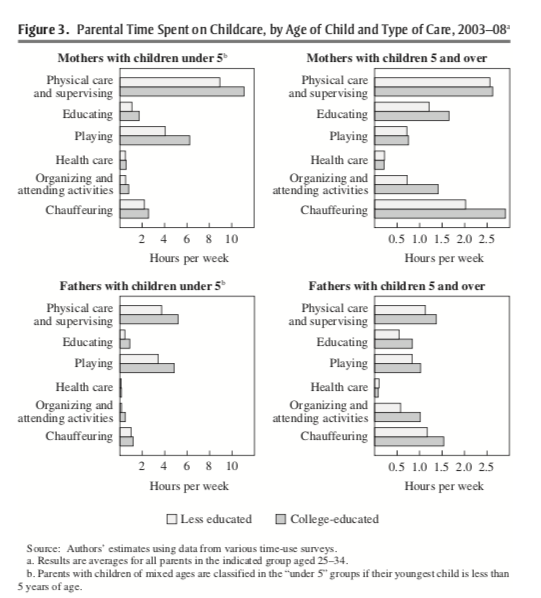
\includegraphics[width=0.9\linewidth]{images/07_ChildCareByType} 

}

\caption{Time Spent on Childcare, by Age of Child and Type of Care 2003-2008 }\label{fig:timebreakdown}
\end{figure}

Let's focus on the top-right panel: mothers with children above the age of 5. College-educated mothers (the darker gray bars) are spending more time on a few categories: education, organizing and attending activities, and chauffeuring. Ramey and Ramey (2010) argue that these may be driven by college competitiveness. To be competitive in college, students need to earn higher scores on tests and participate in more extracurricular activities.

In our data, we are going to create a variable named \texttt{childcollegeprep} that is the sum total of time spent on education and time spent on travelling with children. Right now, however, our data set does not have this variable. So in order to add this, we will need to learn how to create variables in R.

There are two ways to create new variables in R. The first uses base R. The general syntax is:

\begin{Shaded}
\begin{Highlighting}[]
\NormalTok{df}\SpecialCharTok{$}\NormalTok{newvarname }\OtherTok{\textless{}{-}}\NormalTok{ expression}
\end{Highlighting}
\end{Shaded}

For example, let's add the variable \texttt{childcollegeprep} which will be the addition of \texttt{childeduc} and \texttt{childtravel}, which are two variables in our \texttt{rugratrace.csv} data set.

\begin{Shaded}
\begin{Highlighting}[]
\NormalTok{rr}\SpecialCharTok{$}\NormalTok{childcollegeprep }\OtherTok{\textless{}{-}}\NormalTok{ rr}\SpecialCharTok{$}\NormalTok{childeduc }\SpecialCharTok{+}\NormalTok{ rr}\SpecialCharTok{$}\NormalTok{childtravel}
\FunctionTok{summary}\NormalTok{(rr}\SpecialCharTok{$}\NormalTok{childcollegeprep)}
\NormalTok{   Min. }\DecValTok{1}\NormalTok{st Qu.  Median    Mean }\DecValTok{3}\NormalTok{rd Qu.    Max.    NA}\StringTok{\textquotesingle{}s }
\StringTok{  0.000   0.000   0.000   1.201   0.000  98.933    1146 }
\end{Highlighting}
\end{Shaded}

So the mean amount of time spent on \texttt{childcollegprep} is about 1.2 hours. Recall we haven't made any restrictions on \texttt{rr}, so this includes everyone in the data set, including those who don't have children. This explains why the value is so much lower than the values we have been studying for mothers with children in the house.

We can also generate new variables using the \texttt{mutate()} function (from tidyverse). The general syntax is:

\begin{Shaded}
\begin{Highlighting}[]
\FunctionTok{mutate}\NormalTok{(dataframe, }\AttributeTok{newvarname =}\NormalTok{ expression)}
\end{Highlighting}
\end{Shaded}

For example, if we want to add \texttt{childprep} using \texttt{mutate()} we can type:

\begin{Shaded}
\begin{Highlighting}[]
\NormalTok{rr }\OtherTok{\textless{}{-}} \FunctionTok{mutate}\NormalTok{(rr, }\AttributeTok{childcollegeprep=}\NormalTok{childtravel}\SpecialCharTok{+}\NormalTok{childeduc)}
\end{Highlighting}
\end{Shaded}

Note that the first step was to type \texttt{rr\ \textless{}-}. If you don't overwrite \texttt{rr} by specifying this step, R will generate a new tibble with the added variable, but it won't be saved anywhere.

A nice thing about \texttt{mutate()} relative to base R is that you can generate a number of variables within the same \texttt{mutate()} command. For example, imagine we also want to create a variable that captures childcare time not spent on college prep. In other words, we want to add the variable \texttt{childnotcollegeprep\ =\ childtot\ -\ childcollegeprep} to the tibble. We can do this using the following:

\begin{Shaded}
\begin{Highlighting}[]
\NormalTok{rr }\OtherTok{\textless{}{-}} \FunctionTok{mutate}\NormalTok{(rr, }\AttributeTok{childcollegeprep=}\NormalTok{childtravel}\SpecialCharTok{+}\NormalTok{childeduc,}
             \AttributeTok{childnotcollegeprep=}\NormalTok{childtot}\SpecialCharTok{{-}}\NormalTok{childcollegeprep)}
\end{Highlighting}
\end{Shaded}

If you have more variables to add or change, you can simply add a comma to the end of the last line, and add the new variable below. Note, we can even call variables that are created earlier in the function (i.e.~\texttt{childnotcollegeprep} can only be created if \texttt{childcollegeprep} is created first).

Lastly, let's talk about the \texttt{transmute()} function. This function also generates new variables, but at the same time, it drops all pre-existing variables. For example, if you wanted to create a tibble that only contains \texttt{childcollegeprep} and \texttt{childnotcollegeprep}, you could use the \texttt{transmute()} function:

\begin{Shaded}
\begin{Highlighting}[]
\NormalTok{collegeprepdat }\OtherTok{\textless{}{-}} \FunctionTok{transmute}\NormalTok{(rr,}
                            \AttributeTok{childcollegeprep =}\NormalTok{ childeduc }\SpecialCharTok{+}\NormalTok{ childtravel,}
                            \AttributeTok{childnotcollegeprep =}\NormalTok{ childtot }\SpecialCharTok{{-}}\NormalTok{ childcollegeprep)}
\end{Highlighting}
\end{Shaded}

\begin{Shaded}
\begin{Highlighting}[]
\NormalTok{collegeprepdat}
\CommentTok{\# A tibble: 106,020 x 2}
\NormalTok{   childcollegeprep childnotcollegeprep}
              \SpecialCharTok{\textless{}}\NormalTok{dbl}\SpecialCharTok{\textgreater{}}               \ErrorTok{\textless{}}\NormalTok{dbl}\SpecialCharTok{\textgreater{}}
 \DecValTok{1}            \DecValTok{0}                    \DecValTok{7}   
 \DecValTok{2}            \FloatTok{3.5}                  \FloatTok{1.17}
 \DecValTok{3}            \FloatTok{0.583}                \FloatTok{2.33}
 \DecValTok{4}            \DecValTok{0}                   \FloatTok{42.6} 
 \DecValTok{5}            \DecValTok{0}                    \FloatTok{7.58}
 \DecValTok{6}            \DecValTok{0}                   \FloatTok{27.2} 
 \DecValTok{7}            \FloatTok{1.17}                 \FloatTok{3.03}
 \DecValTok{8}            \DecValTok{0}                    \DecValTok{0}   
 \DecValTok{9}            \DecValTok{0}                    \DecValTok{0}   
\DecValTok{10}            \DecValTok{0}                    \DecValTok{7}   
\CommentTok{\# i 106,010 more rows}
\end{Highlighting}
\end{Shaded}

As you can see, this is a data set that only contains the two variables we created using \texttt{transmute()}.

\section{Group By and Summarize}\label{group-by-and-summarize}

Often in the course of our data analysis we will want to break down some summary statistics by some groups. For example, maybe we have a dataset on individual-level voting records and want to compute average voting rates by state. Maybe we have data on wages over time, and we want to compute the average wage by year. In R, a convenient way to make this calculation is by combing the \texttt{group\_by()} function with the \texttt{summarize()} function.

To begin our discussion of these functions, we will first illustrate how to use the \texttt{summarize()} command before combining it with \texttt{group\_by()}. Our application will again utilize the data from Ramey and Ramey (2010) on time use.

To remind you, the tibble \texttt{rr} contains the year of the observation in a variable named \texttt{dataset} and the amount spent on childcare in a variable named \texttt{childtot}.

\begin{Shaded}
\begin{Highlighting}[]
\FunctionTok{head}\NormalTok{(rr}\SpecialCharTok{$}\NormalTok{dataset)}
\NormalTok{[}\DecValTok{1}\NormalTok{] }\DecValTok{1965} \DecValTok{1965} \DecValTok{1965} \DecValTok{1965} \DecValTok{1965} \DecValTok{1965}
\end{Highlighting}
\end{Shaded}

\begin{Shaded}
\begin{Highlighting}[]
\FunctionTok{head}\NormalTok{(rr}\SpecialCharTok{$}\NormalTok{childtot)}
\NormalTok{[}\DecValTok{1}\NormalTok{]  }\FloatTok{7.000000}  \FloatTok{4.666667}  \FloatTok{2.916667} \FloatTok{42.583332}  \FloatTok{7.583333}
\NormalTok{[}\DecValTok{6}\NormalTok{] }\FloatTok{27.183332}
\end{Highlighting}
\end{Shaded}

The \texttt{summarize()} function is used to generate summary statistics. For example, imagine I just want to take the average level of \texttt{childtot} across the entire sample. We can do this by typing:

\begin{Shaded}
\begin{Highlighting}[]
\FunctionTok{summarize}\NormalTok{(rr, }\AttributeTok{meanchildtot =} \FunctionTok{mean}\NormalTok{(childtot, }\AttributeTok{na.rm=}\NormalTok{T))}
\CommentTok{\# A tibble: 1 x 1}
\NormalTok{  meanchildtot}
         \SpecialCharTok{\textless{}}\NormalTok{dbl}\SpecialCharTok{\textgreater{}}
\DecValTok{1}         \FloatTok{4.69}
\end{Highlighting}
\end{Shaded}

The first part of the code, \texttt{summarize(rr,} tells R that we are generating summary statistics from the \texttt{rr} data set. The second, part \texttt{meanchildtot=} is actually giving a name to the summary statistic. In other words, you can change this part of the code and the only difference will be the name on the column that is output. The actual code will still execute without error. This is a helpful feature of the \texttt{summarize()} command because often we will want to save our summary statistics in a new tibble. If there are multiple summary statistics computed, we need to be able to keep track of the various summary statistics. The last part of the code \texttt{mean(childtot,\ na.rm=T)} is declaring that \texttt{meanchildtot} will be equal to the average of \texttt{childtot}. Because we have specified \texttt{na.rm=T}, missing values are ignored in the computation.

A nice feature of the \texttt{summarize} function is that we can generate multiple statistics in a single line. For example, imagine we would like to compute both the mean level of childcare and the median level of childcare. We can simply add this code to the previous summary command by giving the median a different name:

\begin{Shaded}
\begin{Highlighting}[]
\FunctionTok{summarize}\NormalTok{(rr, }
          \AttributeTok{meanchildtot =} \FunctionTok{mean}\NormalTok{(childtot, }\AttributeTok{na.rm=}\NormalTok{T),}
          \AttributeTok{medianchildtot=}\FunctionTok{median}\NormalTok{(childtot, }\AttributeTok{na.rm =}\NormalTok{ T))}
\CommentTok{\# A tibble: 1 x 2}
\NormalTok{  meanchildtot medianchildtot}
         \SpecialCharTok{\textless{}}\NormalTok{dbl}\SpecialCharTok{\textgreater{}}          \ErrorTok{\textless{}}\NormalTok{dbl}\SpecialCharTok{\textgreater{}}
\DecValTok{1}         \FloatTok{4.69}              \DecValTok{0}
\end{Highlighting}
\end{Shaded}

The median is actually zero here because we are taking the median for the entire sample. Many individuals will have zero time spent on childcare, as there aren't any children in many households.

Next, we will discuss the real usefulness of the summarize command: summarizing by groups. Many times as part of our analysis, we might want to provide summary statistics over some group variable. At other times, we may actually want to change the unit-of-observation of our dataset. Using the \texttt{group\_by()} function with the \texttt{summarize()} function is a convenient way to accomplish this.

The \texttt{group\_by()} function tells R that any subsequent functions should be done separately by the values of the \texttt{group\_by()} variable. For example, in our dataset, we have a list of years:

\begin{Shaded}
\begin{Highlighting}[]
\FunctionTok{unique}\NormalTok{(rr}\SpecialCharTok{$}\NormalTok{dataset)}
\NormalTok{ [}\DecValTok{1}\NormalTok{] }\DecValTok{1965} \DecValTok{1975} \DecValTok{1985} \DecValTok{1993}   \ConstantTok{NA} \DecValTok{1995} \DecValTok{1998} \DecValTok{2000} \DecValTok{2003} \DecValTok{2004} \DecValTok{2005}
\NormalTok{[}\DecValTok{12}\NormalTok{] }\DecValTok{2006} \DecValTok{2007} \DecValTok{2008}
\end{Highlighting}
\end{Shaded}

Therefore, if we specify \texttt{group\_by(dataset)}, then subsequent functions will be applied separately by each value of \texttt{dataset}. In particular, if we next \texttt{summarize(meanchildtot\ =\ mean(childtot,\ na.rm=T))}, then the mean of \texttt{childtot} will be taken separately for each value of \texttt{dataset}. Let's try this all together now.

\begin{Shaded}
\begin{Highlighting}[]
\NormalTok{rr }\SpecialCharTok{\%\textgreater{}\%}
  \FunctionTok{group\_by}\NormalTok{(dataset) }\SpecialCharTok{\%\textgreater{}\%}
  \FunctionTok{summarize}\NormalTok{(}\AttributeTok{meanchildtot=}\FunctionTok{mean}\NormalTok{(childtot,}\AttributeTok{na.rm=}\NormalTok{T))}
\end{Highlighting}
\end{Shaded}

\begin{verbatim}
# A tibble: 14 x 2
   dataset meanchildtot
     <dbl>        <dbl>
 1    1965         4.27
 2    1975         3.36
 3    1985         2.95
 4    1993         2.09
 5    1995         4.23
 6    1998         5.20
 7    2000        10.5 
 8    2003         4.85
 9    2004         4.73
10    2005         5.17
11    2006         5.06
12    2007         4.92
13    2008         4.97
14      NA       NaN   
\end{verbatim}

The way we can read the code above is: first read in \texttt{rr} tibble, and then group by values of the variable \texttt{dataset}, and then for each value of \texttt{dataset}, take the average of \texttt{childtot}, and store this information under the name \texttt{meanchildtot}.

We can also make this even more complicated by summarizing by two variables. If you type \texttt{group\_by(var1,var2)}, then R will group by the unique combination of variables. Before proceeding to the main example, let's generate a small data frame through which we can understand grouping by two variables.

\begin{Shaded}
\begin{Highlighting}[]
\NormalTok{student.df }\OtherTok{\textless{}{-}} \FunctionTok{data.frame}\NormalTok{(}\AttributeTok{school=}\FunctionTok{c}\NormalTok{(}\StringTok{"A"}\NormalTok{, }\StringTok{"A"}\NormalTok{, }\StringTok{"A"}\NormalTok{, }\StringTok{"B"}\NormalTok{, }\StringTok{"B"}\NormalTok{, }\StringTok{"B"}\NormalTok{),}
                        \AttributeTok{graduationdate=}\FunctionTok{c}\NormalTok{(}\DecValTok{2010}\NormalTok{,}\DecValTok{2010}\NormalTok{,}\DecValTok{2015}\NormalTok{,}\DecValTok{2010}\NormalTok{,}\DecValTok{2010}\NormalTok{,}\DecValTok{2015}\NormalTok{),}
                        \AttributeTok{gpa =} \FunctionTok{c}\NormalTok{(}\FloatTok{3.2}\NormalTok{,}\FloatTok{3.7}\NormalTok{,}\FloatTok{2.9}\NormalTok{,}\FloatTok{4.0}\NormalTok{,}\FloatTok{3.2}\NormalTok{,}\FloatTok{1.8}\NormalTok{))}
\end{Highlighting}
\end{Shaded}

\begin{Shaded}
\begin{Highlighting}[]
\NormalTok{student.df}
\NormalTok{  school graduationdate gpa}
\DecValTok{1}\NormalTok{      A           }\DecValTok{2010} \FloatTok{3.2}
\DecValTok{2}\NormalTok{      A           }\DecValTok{2010} \FloatTok{3.7}
\DecValTok{3}\NormalTok{      A           }\DecValTok{2015} \FloatTok{2.9}
\DecValTok{4}\NormalTok{      B           }\DecValTok{2010} \FloatTok{4.0}
\DecValTok{5}\NormalTok{      B           }\DecValTok{2010} \FloatTok{3.2}
\DecValTok{6}\NormalTok{      B           }\DecValTok{2015} \FloatTok{1.8}
\end{Highlighting}
\end{Shaded}

If I type \texttt{group\_by(school,graduationdate)}, then any subsequent \texttt{summarize()} command will be done completely separately by unique combinations of \texttt{school} and \texttt{graduationdate}. In this data frame, there are 4 unique combinations -- ``A 2010'', ``A 2015'', ``B 2010'', ``B 2015''. So let's see what we get when we summarize by groups of two variables:

\begin{Shaded}
\begin{Highlighting}[]
\NormalTok{student.df }\SpecialCharTok{\%\textgreater{}\%} 
  \FunctionTok{group\_by}\NormalTok{(school,graduationdate) }\SpecialCharTok{\%\textgreater{}\%}
  \FunctionTok{summarize}\NormalTok{(}\AttributeTok{mean.gpa=}\FunctionTok{mean}\NormalTok{(gpa))}
\StringTok{\textasciigrave{}}\AttributeTok{summarise()}\StringTok{\textasciigrave{}}\NormalTok{ has regrouped the output.}
\NormalTok{i Summaries were computed grouped by school and}
\NormalTok{  graduationdate.}
\NormalTok{i Output is grouped by school.}
\NormalTok{i Use }\StringTok{\textasciigrave{}}\AttributeTok{summarise(.groups = "drop\_last")}\StringTok{\textasciigrave{}}\NormalTok{ to silence this}
\NormalTok{  message.}
\NormalTok{i Use }\StringTok{\textasciigrave{}}\AttributeTok{summarise(.by = c(school, graduationdate))}\StringTok{\textasciigrave{}} \ControlFlowTok{for}
\NormalTok{  per}\SpecialCharTok{{-}}\NormalTok{operation }\FunctionTok{grouping}\NormalTok{ (}\StringTok{\textasciigrave{}}\AttributeTok{?dplyr::dplyr\_by}\StringTok{\textasciigrave{}}\NormalTok{) instead.}
\CommentTok{\# A tibble: 4 x 3}
\CommentTok{\# Groups:   school [2]}
\NormalTok{  school graduationdate mean.gpa}
  \SpecialCharTok{\textless{}}\NormalTok{chr}\SpecialCharTok{\textgreater{}}           \ErrorTok{\textless{}}\NormalTok{dbl}\SpecialCharTok{\textgreater{}}    \ErrorTok{\textless{}}\NormalTok{dbl}\SpecialCharTok{\textgreater{}}
\DecValTok{1}\NormalTok{ A                }\DecValTok{2010}     \FloatTok{3.45}
\DecValTok{2}\NormalTok{ A                }\DecValTok{2015}     \FloatTok{2.9} 
\DecValTok{3}\NormalTok{ B                }\DecValTok{2010}     \FloatTok{3.6} 
\DecValTok{4}\NormalTok{ B                }\DecValTok{2015}     \FloatTok{1.8} 
\end{Highlighting}
\end{Shaded}

To understand how the unique combinations are generated, let's change the dataset slightly.

\begin{Shaded}
\begin{Highlighting}[]
\NormalTok{student.df }\OtherTok{\textless{}{-}} \FunctionTok{data.frame}\NormalTok{(}\AttributeTok{school=}\FunctionTok{c}\NormalTok{(}\StringTok{"A"}\NormalTok{, }\StringTok{"A"}\NormalTok{, }\StringTok{"A"}\NormalTok{, }\StringTok{"B"}\NormalTok{, }\StringTok{"B"}\NormalTok{, }\StringTok{"B"}\NormalTok{),}
                        \AttributeTok{graduationdate=}\FunctionTok{c}\NormalTok{(}\DecValTok{2010}\NormalTok{,}\DecValTok{2010}\NormalTok{,}\DecValTok{2010}\NormalTok{,}\DecValTok{2015}\NormalTok{,}\DecValTok{2015}\NormalTok{,}\DecValTok{2015}\NormalTok{),}
                        \AttributeTok{gpa =} \FunctionTok{c}\NormalTok{(}\FloatTok{3.2}\NormalTok{,}\FloatTok{3.7}\NormalTok{,}\FloatTok{2.9}\NormalTok{,}\FloatTok{4.0}\NormalTok{,}\FloatTok{3.2}\NormalTok{,}\FloatTok{1.8}\NormalTok{))}
\end{Highlighting}
\end{Shaded}

Now there are only two unique combinations in the data of school and graduation date: ``A 2010'' and ``B 2015''. Therefore, when we summarize by groups, there will be only two averages taken:

\begin{Shaded}
\begin{Highlighting}[]
\NormalTok{student.df }\SpecialCharTok{\%\textgreater{}\%} 
  \FunctionTok{group\_by}\NormalTok{(school,graduationdate) }\SpecialCharTok{\%\textgreater{}\%}
  \FunctionTok{summarize}\NormalTok{(}\AttributeTok{mean.gpa=}\FunctionTok{mean}\NormalTok{(gpa))}
\CommentTok{\# A tibble: 2 x 3}
\CommentTok{\# Groups:   school [2]}
\NormalTok{  school graduationdate mean.gpa}
  \SpecialCharTok{\textless{}}\NormalTok{chr}\SpecialCharTok{\textgreater{}}           \ErrorTok{\textless{}}\NormalTok{dbl}\SpecialCharTok{\textgreater{}}    \ErrorTok{\textless{}}\NormalTok{dbl}\SpecialCharTok{\textgreater{}}
\DecValTok{1}\NormalTok{ A                }\DecValTok{2010}     \FloatTok{3.27}
\DecValTok{2}\NormalTok{ B                }\DecValTok{2015}     \DecValTok{3}   
\end{Highlighting}
\end{Shaded}

Now, let's return to the \texttt{rr} tibble. In Ramey and Ramey (2010), the authors compared time spent on childcare over time separately for college-educated and less-than-college educated individuals. We can achieve a similar analysis by grouping over \texttt{dataset} and \texttt{college}. The variable \texttt{college} is a variable that takes on a value of 1 if the individual graduated from college, and zero otherwise.

\begin{Shaded}
\begin{Highlighting}[]
\NormalTok{rr }\SpecialCharTok{\%\textgreater{}\%}
  \FunctionTok{group\_by}\NormalTok{(dataset,college) }\SpecialCharTok{\%\textgreater{}\%}
  \FunctionTok{summarize}\NormalTok{(}\AttributeTok{meanchildtot =} \FunctionTok{mean}\NormalTok{(childtot, }\AttributeTok{na.rm=}\NormalTok{T))}
\CommentTok{\# A tibble: 27 x 3}
\CommentTok{\# Groups:   dataset [14]}
\NormalTok{   dataset college meanchildtot}
     \SpecialCharTok{\textless{}}\NormalTok{dbl}\SpecialCharTok{\textgreater{}}   \ErrorTok{\textless{}}\NormalTok{dbl}\SpecialCharTok{\textgreater{}}        \ErrorTok{\textless{}}\NormalTok{dbl}\SpecialCharTok{\textgreater{}}
 \DecValTok{1}    \DecValTok{1965}       \DecValTok{0}         \FloatTok{4.35}
 \DecValTok{2}    \DecValTok{1965}       \DecValTok{1}         \FloatTok{3.66}
 \DecValTok{3}    \DecValTok{1975}       \DecValTok{0}         \FloatTok{3.33}
 \DecValTok{4}    \DecValTok{1975}       \DecValTok{1}         \FloatTok{3.51}
 \DecValTok{5}    \DecValTok{1985}       \DecValTok{0}         \FloatTok{2.89}
 \DecValTok{6}    \DecValTok{1985}       \DecValTok{1}         \FloatTok{3.13}
 \DecValTok{7}    \DecValTok{1993}       \DecValTok{0}         \FloatTok{2.25}
 \DecValTok{8}    \DecValTok{1993}       \DecValTok{1}         \FloatTok{1.74}
 \DecValTok{9}    \DecValTok{1995}       \DecValTok{0}         \FloatTok{4.39}
\DecValTok{10}    \DecValTok{1995}       \DecValTok{1}         \FloatTok{3.85}
\CommentTok{\# i 17 more rows}
\end{Highlighting}
\end{Shaded}

To understand this table, let's look at the first row of data. This first row has \texttt{dataset==1965} and \texttt{college==0}. In other words, this row corresponds to individuals in 1965 without a college education. The value in the \texttt{meanchildtot} column is the average amount of time spent on childcare for these individuals. If we move down this table, we will see R has computed the mean time spent on childcare for every unique combination of \texttt{dataset} and \texttt{college}.

Often in practice, we may want to actually save the output of this function. To do so, we just need to assign it a name, as usual:

\begin{Shaded}
\begin{Highlighting}[]
\NormalTok{totchildbyyearcollege }\OtherTok{\textless{}{-}}\NormalTok{ rr }\SpecialCharTok{\%\textgreater{}\%}
  \FunctionTok{group\_by}\NormalTok{(dataset, college) }\SpecialCharTok{\%\textgreater{}\%}
  \FunctionTok{summarize}\NormalTok{(}\AttributeTok{meanchildtot =} \FunctionTok{mean}\NormalTok{(childtot, }\AttributeTok{na.rm=}\NormalTok{T))}
\end{Highlighting}
\end{Shaded}

Now we have created a new tibble \texttt{totchildbyyearcollege} that contains these averages over time by college education.

We could have also accomplished this by looping over values of dataset and college and then computing the means and storing them. But doing so would have included (1) writing much more code and (2) would have actually taken longer to run. Using \texttt{group\_by()} with \texttt{summarize()} is a much more efficient way to accomplish this.

\section{Conclusion}\label{conclusion-5}

In this final section we will put all the various functions we've learned together into one analysis. As a reminder, our goal is to compute the average time spent on childcare for mothers over time, separately by college-education status. In other words, replicate Figure \ref{fig:rugrat} from Ramey and Ramey (2010) which shows increased time spent on childcare beginning in the 1990s, especially for college-educated mothers.

This review will focus on the \texttt{tidyverse} package. As a reminder, the first time using a package you need to install it using \texttt{install.packages("packagename")}. You only need to do this once. However, every time you want to use the package in a given R session, you need to load it into memory using the \texttt{library()} function. For example, to load tidyverse we would type:

\begin{Shaded}
\begin{Highlighting}[]
\FunctionTok{library}\NormalTok{(tidyverse)}
\end{Highlighting}
\end{Shaded}

To begin, let's first re-load our data into R as a tibble using the \texttt{read\_csv()} function. The \texttt{read\_csv()} function reads in a dataset as a tibble, while the \texttt{read.csv()} function reads the dataset into memory as a data frame. For our purposes, there won't be too much differences between these formats, but tibbles will be more efficient with large datasets.

\begin{Shaded}
\begin{Highlighting}[]
\NormalTok{rr }\OtherTok{\textless{}{-}} \FunctionTok{read\_csv}\NormalTok{(}\StringTok{"rugratrace.csv"}\NormalTok{)}
\NormalTok{Rows}\SpecialCharTok{:} \DecValTok{106020}\NormalTok{ Columns}\SpecialCharTok{:} \DecValTok{54}
\SpecialCharTok{{-}{-}}\NormalTok{ Column specification }\SpecialCharTok{{-}{-}{-}{-}{-}{-}{-}{-}{-}{-}{-}{-}{-}{-}{-}{-}{-}{-}{-}{-}{-}{-}{-}{-}{-}{-}{-}{-}{-}{-}{-}{-}{-}{-}{-}{-}}
\NormalTok{Delimiter}\SpecialCharTok{:} \StringTok{","}
\FunctionTok{dbl}\NormalTok{ (}\DecValTok{54}\NormalTok{)}\SpecialCharTok{:}\NormalTok{ state, age, sex, ethnic, under18, under5, agey...}

\NormalTok{i Use }\StringTok{\textasciigrave{}}\AttributeTok{spec()}\StringTok{\textasciigrave{}}\NormalTok{ to retrieve the full column specification }\ControlFlowTok{for}\NormalTok{ this data.}
\NormalTok{i Specify the column types or set }\StringTok{\textasciigrave{}}\AttributeTok{show\_col\_types = FALSE}\StringTok{\textasciigrave{}}\NormalTok{ to quiet this message.}
\end{Highlighting}
\end{Shaded}

Our first issue is that the Ramey and Ramey (2010) analysis was for a particular group of individuals: mothers aged 25-34. Therefore, we first need to create a dataset restricted to these individuals. We can achieve this by using the \texttt{filter()} function.

\begin{Shaded}
\begin{Highlighting}[]
\NormalTok{mothers2534 }\OtherTok{\textless{}{-}} \FunctionTok{filter}\NormalTok{(rr, mother2}\SpecialCharTok{==}\DecValTok{1}\NormalTok{, age}\SpecialCharTok{\textgreater{}}\DecValTok{24}\NormalTok{, age}\SpecialCharTok{\textless{}}\DecValTok{35}\NormalTok{)}
\end{Highlighting}
\end{Shaded}

Now, a focus of our analysis will be what is driving the increase in time spent on childcare. One potential driver is increased time spent on college prep activities, given an increase in the competitiveness of college during this time. We are going to add a variable named \texttt{collegeprep} to this dataset which is the time spent either on traveling with children or time spent educating children.

\begin{Shaded}
\begin{Highlighting}[]
\NormalTok{mothers\_collegeprep }\OtherTok{\textless{}{-}} \FunctionTok{mutate}\NormalTok{(mothers2534, }
                              \AttributeTok{collegeprep =}\NormalTok{ childeduc }\SpecialCharTok{+}\NormalTok{ childtravel)}
\end{Highlighting}
\end{Shaded}

Our goal is to compute the amount of time spent on \texttt{collegeprep} over time, by college education status. We can accomplish this by using \texttt{group\_by()} and \texttt{summarize()} functions together.

\begin{Shaded}
\begin{Highlighting}[]
\NormalTok{collegeprep }\OtherTok{\textless{}{-}}\NormalTok{ mothers\_collegeprep }\SpecialCharTok{\%\textgreater{}\%}
  \FunctionTok{group\_by}\NormalTok{(dataset, college) }\SpecialCharTok{\%\textgreater{}\%}
  \FunctionTok{summarize}\NormalTok{(}\AttributeTok{meancollegeprep=}\FunctionTok{mean}\NormalTok{(collegeprep, }\AttributeTok{na.rm=}\NormalTok{T))}
\StringTok{\textasciigrave{}}\AttributeTok{summarise()}\StringTok{\textasciigrave{}}\NormalTok{ has regrouped the output.}
\NormalTok{i Summaries were computed grouped by dataset and college.}
\NormalTok{i Output is grouped by dataset.}
\NormalTok{i Use }\StringTok{\textasciigrave{}}\AttributeTok{summarise(.groups = "drop\_last")}\StringTok{\textasciigrave{}}\NormalTok{ to silence this}
\NormalTok{  message.}
\NormalTok{i Use }\StringTok{\textasciigrave{}}\AttributeTok{summarise(.by = c(dataset, college))}\StringTok{\textasciigrave{}} \ControlFlowTok{for}
\NormalTok{  per}\SpecialCharTok{{-}}\NormalTok{operation }\FunctionTok{grouping}\NormalTok{ (}\StringTok{\textasciigrave{}}\AttributeTok{?dplyr::dplyr\_by}\StringTok{\textasciigrave{}}\NormalTok{) instead.}
\end{Highlighting}
\end{Shaded}

Now if we look at our resulting tibble, we can use it to understand trends in time spent on college prep over time:

\begin{Shaded}
\begin{Highlighting}[]
\FunctionTok{print}\NormalTok{(collegeprep,}\AttributeTok{n=}\DecValTok{25}\NormalTok{)}
\CommentTok{\# A tibble: 22 x 3}
\CommentTok{\# Groups:   dataset [11]}
\NormalTok{   dataset college meancollegeprep}
     \SpecialCharTok{\textless{}}\NormalTok{dbl}\SpecialCharTok{\textgreater{}}   \ErrorTok{\textless{}}\NormalTok{dbl}\SpecialCharTok{\textgreater{}}           \ErrorTok{\textless{}}\NormalTok{dbl}\SpecialCharTok{\textgreater{}}
 \DecValTok{1}    \DecValTok{1965}       \DecValTok{0}            \FloatTok{2.14}
 \DecValTok{2}    \DecValTok{1965}       \DecValTok{1}            \FloatTok{1.88}
 \DecValTok{3}    \DecValTok{1975}       \DecValTok{0}            \FloatTok{1.66}
 \DecValTok{4}    \DecValTok{1975}       \DecValTok{1}            \FloatTok{1.69}
 \DecValTok{5}    \DecValTok{1985}       \DecValTok{0}            \FloatTok{2.52}
 \DecValTok{6}    \DecValTok{1985}       \DecValTok{1}            \FloatTok{2.72}
 \DecValTok{7}    \DecValTok{1993}       \DecValTok{0}            \FloatTok{1.49}
 \DecValTok{8}    \DecValTok{1993}       \DecValTok{1}            \FloatTok{1.87}
 \DecValTok{9}    \DecValTok{1998}       \DecValTok{0}            \FloatTok{2.46}
\DecValTok{10}    \DecValTok{1998}       \DecValTok{1}            \FloatTok{2.51}
\DecValTok{11}    \DecValTok{2003}       \DecValTok{0}            \FloatTok{3.27}
\DecValTok{12}    \DecValTok{2003}       \DecValTok{1}            \FloatTok{3.34}
\DecValTok{13}    \DecValTok{2004}       \DecValTok{0}            \FloatTok{2.87}
\DecValTok{14}    \DecValTok{2004}       \DecValTok{1}            \FloatTok{3.72}
\DecValTok{15}    \DecValTok{2005}       \DecValTok{0}            \FloatTok{3.23}
\DecValTok{16}    \DecValTok{2005}       \DecValTok{1}            \FloatTok{3.05}
\DecValTok{17}    \DecValTok{2006}       \DecValTok{0}            \FloatTok{3.00}
\DecValTok{18}    \DecValTok{2006}       \DecValTok{1}            \FloatTok{3.16}
\DecValTok{19}    \DecValTok{2007}       \DecValTok{0}            \FloatTok{3.18}
\DecValTok{20}    \DecValTok{2007}       \DecValTok{1}            \FloatTok{3.30}
\DecValTok{21}    \DecValTok{2008}       \DecValTok{0}            \FloatTok{3.39}
\DecValTok{22}    \DecValTok{2008}       \DecValTok{1}            \FloatTok{3.28}
\end{Highlighting}
\end{Shaded}

What do we find in this data? In the 60s-70s, on average, mothers spent around 1.5-2 hours on activities that may be related to college preparation. This increases over time, and by the 2000s, it has stabilized to closer to 3 hours on average. Therefore, we find something broadly consistent with Ramey and Ramey (2010). Time spent on childcare has increased over time, and in particular, for activities that may be related to college preparation.

Now, one thing to note is that we have done this analysis step-by-step. First we restricted our sample, then we added the variables, and lastly we summarized by group. However, we could have also done this entire analysis in a single block of code by stringing together functions using the pipe operator, as is done below:

\begin{Shaded}
\begin{Highlighting}[]
\NormalTok{collegeprep }\OtherTok{\textless{}{-}}\NormalTok{ rr }\SpecialCharTok{\%\textgreater{}\%}
  \FunctionTok{filter}\NormalTok{(mother2}\SpecialCharTok{==}\DecValTok{1}\NormalTok{, age}\SpecialCharTok{\textgreater{}}\DecValTok{24}\NormalTok{, age}\SpecialCharTok{\textless{}}\DecValTok{35}\NormalTok{) }\SpecialCharTok{\%\textgreater{}\%}
  \FunctionTok{mutate}\NormalTok{(}\AttributeTok{collegeprep =}\NormalTok{ childeduc }\SpecialCharTok{+}\NormalTok{ childtravel) }\SpecialCharTok{\%\textgreater{}\%}
  \FunctionTok{group\_by}\NormalTok{(dataset, college) }\SpecialCharTok{\%\textgreater{}\%}
  \FunctionTok{summarize}\NormalTok{(}\AttributeTok{meancollegeprep=}\FunctionTok{mean}\NormalTok{(collegeprep, }\AttributeTok{na.rm=}\NormalTok{T))}
\StringTok{\textasciigrave{}}\AttributeTok{summarise()}\StringTok{\textasciigrave{}}\NormalTok{ has regrouped the output.}
\NormalTok{i Summaries were computed grouped by dataset and college.}
\NormalTok{i Output is grouped by dataset.}
\NormalTok{i Use }\StringTok{\textasciigrave{}}\AttributeTok{summarise(.groups = "drop\_last")}\StringTok{\textasciigrave{}}\NormalTok{ to silence this}
\NormalTok{  message.}
\NormalTok{i Use }\StringTok{\textasciigrave{}}\AttributeTok{summarise(.by = c(dataset, college))}\StringTok{\textasciigrave{}} \ControlFlowTok{for}
\NormalTok{  per}\SpecialCharTok{{-}}\NormalTok{operation }\FunctionTok{grouping}\NormalTok{ (}\StringTok{\textasciigrave{}}\AttributeTok{?dplyr::dplyr\_by}\StringTok{\textasciigrave{}}\NormalTok{) instead.}
\end{Highlighting}
\end{Shaded}

Going forward in the book, the tools we have learned in this section will be very important. It is extremely common to need to perform some data wrangling steps before proceeding to your actual analysis. The tidyverse package has given us a convenient set of functions in order to perform this analysis.

\section*{Function Descriptions}\label{function-descriptions-1}
\addcontentsline{toc}{section}{Function Descriptions}

\textbf{Tidyverse Functions}

\begin{itemize}
\item
  \texttt{read\_csv()} -- Reads a csv into memory as a tibble. A tibble is similar to a data frame, but more efficient in many settings.
\item
  \texttt{as\_tibble()} -- Converts a data frame to a tibble.
\item
  \texttt{filter()} -- Restricts to certain observations in a data set. For example, \texttt{filter(df,\ age\textgreater{}18)} would restrict the hypothetical data frame \texttt{df} to individuals with \texttt{age\textgreater{}18}.
\item
  \texttt{arrange()} -- Sorts the data based on the value of a variable. For example, \texttt{arrange(df,\ age)} would sort the dataset \texttt{df} from youngest to oldest.
\item
  \texttt{select()} -- Selects certain variables from a dataset. It can be used to restrict to only the variables needed for your analysis.
\item
  \texttt{mutate()} -- used to generate new variables.
\item
  \texttt{group\_by()} -- Groups data based on values of a variable. Any subsequent commands will be done separately by the values of the variable.
\item
  \texttt{summarize()} -- Used to generate summary statistics. Often combined with \texttt{group\_by()} in order to generate summary statistics by groups.
\item
\end{itemize}

\textbf{Other Functions}

\begin{itemize}
\item
  \texttt{sample()} -- Draws a random number from a list of numbers. For example, \texttt{sample(-1:1,1)} draws a single number from the list of numbers \texttt{-1:1}. In other words, it will draw a random number from -1 to 1. \texttt{sample(c(0,1,2),4)} would draw 4 random numbers from the list of numbers 0,1, or 2.
\item
  \texttt{cat()} -- Concatenates text in R. For example, \texttt{cat("Hello","World")} will yield the phrase ``Hello World''.
\item
  \texttt{unique()} -- Retrieves a list of the unique values a variable takes on.
\end{itemize}

\textbf{Installing/Loading Functions}

\begin{itemize}
\item
  \texttt{install.packages()} -- Installs a package onto your version of R. For example, \texttt{install.packages("tidyverse")} will install the tidyverse into R. You need to install a package once.
\item
  \texttt{library()} -- Loads a package into memory.
\end{itemize}

\chapter{Automated Pollution Monitoring}\label{automated-pollution-monitoring}

\section{Principal Agent Problem}\label{principal-agent-problem}

In economics and political science, there is a concept known as the \textbf{principal agent problem}. This setting arises when there is an agent that is making decisions on behalf of a principal, but the agent and the principal's incentives may not align.

A classic example is employees at a firm. The employee is putting in some amount of effort to produce some output for the firm owner. The firm owner may want to produce as much output as possible, but the employee may balance output with the amount of effort it takes to produce that output. Therefore, their incentives do not necessarily align.

Another classic example is elected officials and the citizenry. The officials make decisions (i.e.~the agents) acting on behalf of the citizens (i.e.~the principal). However, the goal of the elected officials may be to be re-elected, not necessarily make the optimal decisions for the citizens. Therefore, in this setting as well, it is possible that the incentives are not necessarily aligned between the agent and the principal.

In this section, we will be discussing an interesting setting in which the principal agent problem is at play. In China, the central government (the principal) has recently made it a priority to reduce air pollution. To accomplish this, they provide high-power incentives to local governments (the agent) that achieve pollution targets. However, the local government officials are also the ones collecting the pollution data. While it may be costly to reduce air pollution, one possibility is that they can cheat and report pollution numbers lower than the actual pollution level.

Greenstone et al.~(2022)\citep{greenstone2022can} studies this question by examining the introduction of automatic air pollution monitoring in China. This automated system was implemented in order to get accurate measures of pollution that cannot be manipulated by local officials. There are basically two potential outcomes of this analysis. First, local officials were reporting accurate numbers. In this case, we wouldn't expect automatic monitoring to change reported pollution numbers. The numbers are accurate both before and after the policy, and therefore, we expect the levels to be similar both before and after the policy.

The second possibility is that reported levels of pollution increase after automatic monitoring. If this is the case, then it suggests local governments were misreporting before automatic monitoring so that it would appear as if they are meeting pollution targets.

In order to measure pollution we will use reported PM10. This is a measure of particulates in the air that are 10 micrometers in diameter or smaller, and a common metric through which to measure air pollution. The focus of our coding this week will be on creating figures in R. We will create figures in both base R, as well as utilizing a popular graphics package, ggplot2. In the end, we will use our figures to understand whether local officials misreported pollution data in China.

\section{Creating Histograms}\label{creating-histograms}

In this section, we are going to learn how to construct histograms in base R. To begin, we first need to load the data frame. However, the data we will be using \texttt{station\_day\_1116.dta} is a Stata dataset. In the past, we have only loaded in either RData or csv files.

In order to load in a Stata data set we are going to make use of the \texttt{haven} package. In order to install the haven package, you need to execute \texttt{install.packages("haven")}. Then, in your current R session you need to load the package using the \texttt{library()} function. Since we will again be utilizing the tidyverse in this section, we will also load the tidyverse package.

\begin{Shaded}
\begin{Highlighting}[]
\FunctionTok{library}\NormalTok{(haven)}
\FunctionTok{library}\NormalTok{(tidyverse)}
\CommentTok{\#\textgreater{} {-}{-} Attaching core tidyverse packages {-}{-}{-}{-} tidyverse 2.0.0 {-}{-}}
\CommentTok{\#\textgreater{} v dplyr     1.2.0     v readr     2.2.0}
\CommentTok{\#\textgreater{} v forcats   1.0.1     v stringr   1.6.0}
\CommentTok{\#\textgreater{} v ggplot2   4.0.2     v tibble    3.3.1}
\CommentTok{\#\textgreater{} v lubridate 1.9.5     v tidyr     1.3.2}
\CommentTok{\#\textgreater{} v purrr     1.2.1     }
\CommentTok{\#\textgreater{} {-}{-} Conflicts {-}{-}{-}{-}{-}{-}{-}{-}{-}{-}{-}{-}{-}{-}{-}{-}{-}{-}{-}{-}{-}{-} tidyverse\_conflicts() {-}{-}}
\CommentTok{\#\textgreater{} x dplyr::filter() masks stats::filter()}
\CommentTok{\#\textgreater{} x dplyr::lag()    masks stats::lag()}
\CommentTok{\#\textgreater{} i Use the conflicted package (\textless{}http://conflicted.r{-}lib.org/\textgreater{}) to force all conflicts to become errors}
\end{Highlighting}
\end{Shaded}

The \texttt{haven} package comes with a function \texttt{read\_dta}, which will read in a \texttt{.dta} file as a tibble.

\begin{Shaded}
\begin{Highlighting}[]
\NormalTok{pm }\OtherTok{\textless{}{-}} \FunctionTok{read\_dta}\NormalTok{(}\StringTok{"station\_day\_1116.dta"}\NormalTok{)}
\end{Highlighting}
\end{Shaded}

To first get a sense of our data, let's look at a few of the key variables in this dataset.

\begin{Shaded}
\begin{Highlighting}[]
\NormalTok{pm }\SpecialCharTok{\%\textgreater{}\%} \FunctionTok{select}\NormalTok{(pm10\_n,code\_city,date,pm10,auto\_date)}
\CommentTok{\#\textgreater{} \# A tibble: 1,433,568 x 5}
\CommentTok{\#\textgreater{}    pm10\_n code\_city  date  pm10 auto\_date}
\CommentTok{\#\textgreater{}     \textless{}dbl\textgreater{}     \textless{}dbl\textgreater{} \textless{}dbl\textgreater{} \textless{}dbl\textgreater{}     \textless{}dbl\textgreater{}}
\CommentTok{\#\textgreater{}  1     46    440300 18628  NA       19060}
\CommentTok{\#\textgreater{}  2     46    440300 18629  NA       19060}
\CommentTok{\#\textgreater{}  3     46    440300 18630  NA       19060}
\CommentTok{\#\textgreater{}  4     46    440300 18631  NA       19060}
\CommentTok{\#\textgreater{}  5     46    440300 18632  NA       19060}
\CommentTok{\#\textgreater{}  6     46    440300 18633  NA       19060}
\CommentTok{\#\textgreater{}  7     46    440300 18634  70.1     19060}
\CommentTok{\#\textgreater{}  8     46    440300 18635 114.      19060}
\CommentTok{\#\textgreater{}  9     46    440300 18636  62.5     19060}
\CommentTok{\#\textgreater{} 10     46    440300 18637  90.8     19060}
\CommentTok{\#\textgreater{} \# i 1,433,558 more rows}
\end{Highlighting}
\end{Shaded}

The first variable, \texttt{pm10\_n} is the station number. This is the code of the station that took the pollution reading. The next variable \texttt{code\_city} is the code of the city in which the pollution reading was taken. This dataset is a panel dataset, which means there are many observations over time. In this case, we will have readings from the same pollution center over time. The \texttt{date} variable stores information on the date the reading was taken. We will discuss a bit later what the number in this variable means. \texttt{pm10} is our measure of pollution. Lastly, \texttt{auto\_date} is the date of automation. After this date, instead of local governments reporting pollution statistics, pollution statistics were directly reported to the central government.

So for this section our goal is to create a histogram that shows the distribution of \texttt{pm10} across cities. Right now, we have a dataset that is at the station-date level. Each row corresponds to a pollution level at a particular station. We want to transform our data into a dataset that has for every city, the average level of pollution in that city.

The way we can do this is to use \texttt{group\_by()} and \texttt{summarize()}, as we did in the prior chapter. If you recall, when you want to create a tibble of summary statistics by a group, we use \texttt{group\_by()} in combination with \texttt{summarize()}. In this example, the group variable is the \texttt{code\_city} and the summary statistic is the average level of \texttt{pm10}.

\begin{Shaded}
\begin{Highlighting}[]
\NormalTok{pm\_bycity }\OtherTok{\textless{}{-}}\NormalTok{ pm }\SpecialCharTok{\%\textgreater{}\%}
  \FunctionTok{group\_by}\NormalTok{(code\_city) }\SpecialCharTok{\%\textgreater{}\%}
  \FunctionTok{summarize}\NormalTok{(}\AttributeTok{meanpm10 =} \FunctionTok{mean}\NormalTok{(pm10, }\AttributeTok{na.rm=}\NormalTok{T))}
\end{Highlighting}
\end{Shaded}

We have included \texttt{na.rm=T}, because looking through the \texttt{pm10} variable, it appears there is some missing data. Adding \texttt{na.rm=T} indicates we are taking the average over the non-missing values.

So now, for each unique value of \texttt{code\_city}, we have the average of the PM10 level in that city and have saved this information in the tibble \texttt{pm\_bycity}.

To generate histograms in base R, we can use the \texttt{hist()} function. For example, let's generate a histogram of \texttt{pm10}:

\begin{Shaded}
\begin{Highlighting}[]
\FunctionTok{hist}\NormalTok{(pm\_bycity}\SpecialCharTok{$}\NormalTok{meanpm10)}
\end{Highlighting}
\end{Shaded}

\begin{figure}

{\centering 
\includegraphics[width=0.8\linewidth]{08-week8_files/figure-latex/hist1-1} 

}

\caption{Histogram of Average Pollution Levels Across Cities Part 1}\label{fig:hist1}
\end{figure}

First, let's review a histogram. On the horizontal axis, we have our numeric variable \texttt{meanpm10}, which is the average level of \texttt{pm10} in a city. The histogram has binned this variable into discrete intervals. R automatically creates these bins when you use the \texttt{hist()} function. Then, in the vertical axis, the number of cities that fall within that interval is presented. So, for example, if we look at the tallest bin, which is about 80-100, we can see there are about 35 cities with average pollution in that range.

While this presents our information, there is a lot we can do in order to improve this figure. For example, the title right now is not clear. A reader may not know what \texttt{pm\_bycity\$meanpm10} means. As usual, we will want to improve these labels.

To change the axis labels, we can use \texttt{xlab="Horizontal\ Axis\ Name"} and \texttt{ylab="Vertical\ Axis\ Name"}. To add a title, we can use \texttt{main="Title\ Name"}. \texttt{main} is perhaps not the most intuitive name for the options that generates a title, but you can think of it is ``What is the main subject for this plot''. So let's try to re-create our plot with better axes labels and titles.

\begin{Shaded}
\begin{Highlighting}[]
\FunctionTok{hist}\NormalTok{(pm\_bycity}\SpecialCharTok{$}\NormalTok{meanpm10, }
     \AttributeTok{xlab=}\StringTok{"Mean PM10"}\NormalTok{, }
     \AttributeTok{ylab=}\StringTok{"Frequency"}\NormalTok{, }
     \AttributeTok{main=}\StringTok{"Mean PM10 by City"}\NormalTok{)}
\end{Highlighting}
\end{Shaded}

\begin{figure}

{\centering 
\includegraphics[width=0.8\linewidth]{08-week8_files/figure-latex/hist2-1} 

}

\caption{Histogram of Average Pollution Levels Across Cities Part 2}\label{fig:hist2}
\end{figure}

These various options will be useful for many different types of graphs in base R, not just histograms. For example, later we will generate a scatter plot. We can use these same options when generating this alternate type of graph.

Next, let's discuss ways in which we can customize the look of our plot. For example, with histograms, one common way to customize the plot is to change the number of bins that are created. R chooses a default number of bins, but you can manually change this by using the \texttt{breaks} option. If you specify a higher number for \texttt{breaks}, that means you want more bins. If you specify a lower number, that means you want fewer bins.

To illustrate this, we are going to put two plots side-by-side. Learning how to put two plots side-by-side is a generally useful technique as well. Often in academic articles, you might see multiple panels in a figure if the information between the panels is closely related. In our example, we are going to create two plots, one with many bins and another with few bins.

The way to tell R to create multiple plots is to use the function called \texttt{par()}. Within \texttt{par()} you can use an argument called \texttt{mfrow=}. \texttt{mfrow=} tells R how many rows and how many columns you want in your plot. For example, in our example, we want on a single row, two separate figures. You can think of this as a row of figures, but two columns of figures. To specify this in R, you can type \texttt{mfrow=c(1,2)}.

\begin{Shaded}
\begin{Highlighting}[]
\FunctionTok{par}\NormalTok{(}\AttributeTok{mfrow=}\FunctionTok{c}\NormalTok{(}\DecValTok{1}\NormalTok{,}\DecValTok{2}\NormalTok{))}

\CommentTok{\#Smaller bins}
\FunctionTok{hist}\NormalTok{(pm\_bycity}\SpecialCharTok{$}\NormalTok{meanpm10, }\AttributeTok{xlab=}\StringTok{"Mean PM10"}\NormalTok{, }
     \AttributeTok{ylab=}\StringTok{"Frequency"}\NormalTok{, }\AttributeTok{main=}\StringTok{"Mean PM10 by City"}\NormalTok{,}
     \AttributeTok{breaks=}\DecValTok{20}\NormalTok{)}

\CommentTok{\#Larger bins}
\FunctionTok{hist}\NormalTok{(pm\_bycity}\SpecialCharTok{$}\NormalTok{meanpm10, }\AttributeTok{xlab=}\StringTok{"Mean PM10"}\NormalTok{, }
     \AttributeTok{ylab=}\StringTok{"Frequency"}\NormalTok{, }\AttributeTok{main=}\StringTok{"Mean PM10 by City"}\NormalTok{,}
     \AttributeTok{breaks=}\DecValTok{4}\NormalTok{)}
\end{Highlighting}
\end{Shaded}

\begin{figure}

{\centering 
\includegraphics[width=0.9\linewidth]{08-week8_files/figure-latex/hist3-1} 

}

\caption{Histogram of Average Pollution Levels Across Cities Part 3}\label{fig:hist3}
\end{figure}

As you can see, when we specify \texttt{breaks=20}, the histogram function generates many bins. When we specified \texttt{breaks=4}, we retrieve only 4 bins.

So generally there is a trade off in the number of bins you create. In the left plot, we get more fine-grained information about the distribution of \texttt{pm10} across cities. On the right, the information is more aggregated, but perhaps easier to read. In many cases, the default number of bins (i.e.~the choice automatically made by R when you do not specify \texttt{breaks}) is a good choice.

\section{Comparing Histograms}\label{comparing-histograms}

In this section we will discuss how to compare two histograms. In particular, we will plot this distribution of pollution levels (PM10) both before and after the implementation of automatic monitoring

Before we construct these histograms, we need to compute a data frame that contains average pollution levels by city, both before and after automation. We can accomplish this by first constructing a variable \texttt{T} that contains days until automation. Then we can filter to days before automation (\texttt{T\textless{}0}). Similarly, we can create a post-automation data frame by filtering to observations such that \texttt{T\textgreater{}0}. We can accomplish all of this in one step by using the pipe operator:

\begin{Shaded}
\begin{Highlighting}[]
\NormalTok{pm\_bycitybefore }\OtherTok{\textless{}{-}}\NormalTok{ pm }\SpecialCharTok{\%\textgreater{}\%}
  \FunctionTok{mutate}\NormalTok{(}\AttributeTok{T=}\NormalTok{date}\SpecialCharTok{{-}}\NormalTok{auto\_date) }\SpecialCharTok{\%\textgreater{}\%}
  \FunctionTok{filter}\NormalTok{(T}\SpecialCharTok{\textless{}}\DecValTok{0}\NormalTok{) }\SpecialCharTok{\%\textgreater{}\%}
  \FunctionTok{group\_by}\NormalTok{(code\_city) }\SpecialCharTok{\%\textgreater{}\%}
  \FunctionTok{summarize}\NormalTok{(}\AttributeTok{meanpm10 =} \FunctionTok{mean}\NormalTok{(pm10, }\AttributeTok{na.rm=}\ConstantTok{TRUE}\NormalTok{))}
\end{Highlighting}
\end{Shaded}

So let's make sure we understand each line of code. \texttt{pm\ \%\textgreater{}\%} pipes in the data frame \texttt{pm}. \texttt{mutate(T=date-auto\_date)} creates a new variable and adds it to the data frame. The name of this new variable is \texttt{T}. If \texttt{T} is negative, that means \texttt{date} is less than \texttt{auto\_date}. Next \texttt{filter(T\textless{}0)} implies we are restricting to observations before the automation date. Lastly, \texttt{group\_by(code\_city)\ \%\textgreater{}\%\ summarize(meanpm10=mean(pm10,\ na.rm=T))} implies we are taking averages of \texttt{pm10} by city. In the end, we will have a dataset where each observation is a separate city, and we have the average level of \texttt{pm10} in that city before automation. We can use analogous code to construct a city-level dataset that has the average level of \texttt{pm10} after automation.

\begin{Shaded}
\begin{Highlighting}[]
\NormalTok{pm\_bycityafter }\OtherTok{\textless{}{-}}\NormalTok{ pm }\SpecialCharTok{\%\textgreater{}\%} 
  \FunctionTok{mutate}\NormalTok{(}\AttributeTok{T=}\NormalTok{date}\SpecialCharTok{{-}}\NormalTok{auto\_date) }\SpecialCharTok{\%\textgreater{}\%}
  \FunctionTok{filter}\NormalTok{(T }\SpecialCharTok{\textgreater{}} \DecValTok{0}\NormalTok{) }\SpecialCharTok{\%\textgreater{}\%}
   \FunctionTok{group\_by}\NormalTok{(code\_city) }\SpecialCharTok{\%\textgreater{}\%}
  \FunctionTok{summarize}\NormalTok{(}\AttributeTok{meanpm10 =} \FunctionTok{mean}\NormalTok{(pm10, }\AttributeTok{na.rm=}\ConstantTok{TRUE}\NormalTok{))}
\end{Highlighting}
\end{Shaded}

Next, we will create two plots that lie side-by-side. In order to do this, we will again specify \texttt{par(mfrow=c(1,2))} before generating the plots.

\begin{Shaded}
\begin{Highlighting}[]
\FunctionTok{par}\NormalTok{(}\AttributeTok{mfrow=}\FunctionTok{c}\NormalTok{(}\DecValTok{1}\NormalTok{,}\DecValTok{2}\NormalTok{))}

\CommentTok{\#Plot histogram for before}
\FunctionTok{hist}\NormalTok{(pm\_bycitybefore}\SpecialCharTok{$}\NormalTok{meanpm10, }\AttributeTok{xlab=}\StringTok{"MeanPM10"}\NormalTok{, }
  \AttributeTok{ylab=}\StringTok{"Frequency"}\NormalTok{,}
  \AttributeTok{main=}\StringTok{"Before Automation"}\NormalTok{)}

\CommentTok{\#Plot histogram for after}
\FunctionTok{hist}\NormalTok{(pm\_bycityafter}\SpecialCharTok{$}\NormalTok{meanpm10, }\AttributeTok{xlab=}\StringTok{"MeanPM10"}\NormalTok{, }
  \AttributeTok{ylab=}\StringTok{"Frequency"}\NormalTok{,}
  \AttributeTok{main=}\StringTok{"After Automation"}\NormalTok{)}
\end{Highlighting}
\end{Shaded}


\includegraphics[width=0.9\linewidth]{08-week8_files/figure-latex/unnamed-chunk-10-1}

In these plots it is not so easy to compare the two distributions. One reason is that they are not on the same scale. As you can see, the x-axis in the After Automation plot goes up to 200, while in the Before Automation plot it goes up to 150. In order for the two to be directly comparable, we should ensure that both the x-axis and the y-axis have the same scale. We can do this using the \texttt{xlim()} and \texttt{ylim()} functions. In the code below, we specify \texttt{xlim=c(0,250)}. This implies the x-axis will start at 0 and go up to 250. We specify \texttt{ylim=c(0,50)}. This implies the y-axis will start at 0 and go up to 50.

\begin{Shaded}
\begin{Highlighting}[]
\CommentTok{\#Create two panes for plots}
\FunctionTok{par}\NormalTok{(}\AttributeTok{mfrow=}\FunctionTok{c}\NormalTok{(}\DecValTok{1}\NormalTok{,}\DecValTok{2}\NormalTok{))}
\CommentTok{\#Plot histogram for before}
\FunctionTok{hist}\NormalTok{(pm\_bycitybefore}\SpecialCharTok{$}\NormalTok{meanpm10, }\AttributeTok{xlab=}\StringTok{"MeanPM10"}\NormalTok{, }
  \AttributeTok{ylab=}\StringTok{"Frequency"}\NormalTok{,}
  \AttributeTok{main=}\StringTok{"Before automation"}\NormalTok{,}
  \AttributeTok{xlim=}\FunctionTok{c}\NormalTok{(}\DecValTok{0}\NormalTok{,}\DecValTok{250}\NormalTok{), }\AttributeTok{ylim=}\FunctionTok{c}\NormalTok{(}\DecValTok{0}\NormalTok{,}\DecValTok{50}\NormalTok{))}
\CommentTok{\#Plot histogram for after}
\FunctionTok{hist}\NormalTok{(pm\_bycityafter}\SpecialCharTok{$}\NormalTok{meanpm10, }\AttributeTok{xlab=}\StringTok{"MeanPM10"}\NormalTok{, }
  \AttributeTok{ylab=}\StringTok{"Frequency"}\NormalTok{,}
  \AttributeTok{main=}\StringTok{"After automation"}\NormalTok{,}
  \AttributeTok{xlim=}\FunctionTok{c}\NormalTok{(}\DecValTok{0}\NormalTok{,}\DecValTok{250}\NormalTok{), }\AttributeTok{ylim=}\FunctionTok{c}\NormalTok{(}\DecValTok{0}\NormalTok{,}\DecValTok{50}\NormalTok{))}
\end{Highlighting}
\end{Shaded}


\includegraphics[width=0.9\linewidth]{08-week8_files/figure-latex/unnamed-chunk-11-1}

Now we can more clearly compare the two plots. Before automation, many of the pm10 averages seem to be clustered just below 100. After automation, the distribution is more spread out, with many observations above 100, and even some above 200. Before automation, no city had an average level of pm10 above 200. Therefore, it appears as if the distribution of \textbf{reported} pm10 has shifted to the right after automation.

Lastly, we can also add additional information to the plot. For example, it might be helpful to quickly be able to understand how the average level of pm10 varies before and after automation. We can add these numbers to the plots by using the \texttt{lines()} function. The way the lines function works is that you specify \((x_1, x_2)\) and \((y_1,y_2)\). The line starts at the point \((x_1,y_1)\) and ends at \((x_2,y_2)\). Therefore, if we want to have a vertical line at the mean we can specify \texttt{lines(c(mean,mean),c(-10,100))}. We have specified \texttt{c(-10,100)} because these numbers are beyond the limits of the graph. Therefore, the vertical line will appear along the entire graph output. To understand how to build lines on graphs, it is helpful to change the numbers in the code below and see how the results change.

\begin{Shaded}
\begin{Highlighting}[]
\NormalTok{meanbefore }\OtherTok{\textless{}{-}} \FunctionTok{mean}\NormalTok{(pm\_bycitybefore}\SpecialCharTok{$}\NormalTok{meanpm10)}
\NormalTok{meanafter }\OtherTok{\textless{}{-}} \FunctionTok{mean}\NormalTok{(pm\_bycityafter}\SpecialCharTok{$}\NormalTok{meanpm10)}
\CommentTok{\#Create two panes for plots}
\FunctionTok{par}\NormalTok{(}\AttributeTok{mfrow=}\FunctionTok{c}\NormalTok{(}\DecValTok{1}\NormalTok{,}\DecValTok{2}\NormalTok{))}
\CommentTok{\#Plot histogram for before}
\FunctionTok{hist}\NormalTok{(pm\_bycitybefore}\SpecialCharTok{$}\NormalTok{meanpm10, }\AttributeTok{xlab=}\StringTok{"MeanPM10"}\NormalTok{,}
  \AttributeTok{ylab=}\StringTok{"Frequency"}\NormalTok{,}
  \AttributeTok{main=}\StringTok{"Before Automation"}\NormalTok{,}
  \AttributeTok{xlim=}\FunctionTok{c}\NormalTok{(}\DecValTok{0}\NormalTok{,}\DecValTok{250}\NormalTok{), }\AttributeTok{ylim=}\FunctionTok{c}\NormalTok{(}\DecValTok{0}\NormalTok{,}\DecValTok{50}\NormalTok{))}
\FunctionTok{lines}\NormalTok{(}\FunctionTok{c}\NormalTok{(meanbefore, meanbefore), }\FunctionTok{c}\NormalTok{(}\SpecialCharTok{{-}}\DecValTok{10}\NormalTok{, }\DecValTok{100}\NormalTok{), }
  \AttributeTok{lty=}\DecValTok{2}\NormalTok{, }\AttributeTok{col=}\StringTok{"red"}\NormalTok{)}
\CommentTok{\#Plot histogram for after}
\FunctionTok{hist}\NormalTok{(pm\_bycityafter}\SpecialCharTok{$}\NormalTok{meanpm10, }\AttributeTok{xlab=}\StringTok{"MeanPM10"}\NormalTok{, }
  \AttributeTok{ylab=}\StringTok{"Frequency"}\NormalTok{,}
  \AttributeTok{main=}\StringTok{"After Automation"}\NormalTok{,}
  \AttributeTok{xlim=}\FunctionTok{c}\NormalTok{(}\DecValTok{0}\NormalTok{,}\DecValTok{250}\NormalTok{), }\AttributeTok{ylim=}\FunctionTok{c}\NormalTok{(}\DecValTok{0}\NormalTok{,}\DecValTok{50}\NormalTok{))}
\FunctionTok{lines}\NormalTok{(}\FunctionTok{c}\NormalTok{(meanafter, meanafter), }\FunctionTok{c}\NormalTok{(}\SpecialCharTok{{-}}\DecValTok{10}\NormalTok{, }\DecValTok{100}\NormalTok{), }
  \AttributeTok{lty=}\DecValTok{2}\NormalTok{, }\AttributeTok{col=}\StringTok{"red"}\NormalTok{)}
\end{Highlighting}
\end{Shaded}

\pandocbounded{
\includegraphics[keepaspectratio]{08-week8_files/figure-latex/unnamed-chunk-12-1.pdf}}

\section{Boxplots}\label{boxplots}

A box plot is a figure we have not yet seen in this course. Like a histogram, it is informative about the distribution of a variable. In particular, a box plot shows a few key statistics of interest, including the median, the 25th percentile and 75th percentile. It is often helpful when you want to show how the distribution of a variable varies across different groups. For example, maybe you are interested in variation in test scores across different classes in a school. Maybe you are interested in how the distribution of wages across different regions of the U.S. In these types of instances, box plots might be an effective way to present your information.

In our example, we are going to construct a box plot that shows the average daily pm10 levels both before and after automation. To begin, we are again going to use \texttt{group\_by()} and \texttt{summarize()} to construct a relevant dataset.

\begin{Shaded}
\begin{Highlighting}[]
\CommentTok{\#Group by day}
\NormalTok{pm\_byday }\OtherTok{\textless{}{-}}\NormalTok{ pm }\SpecialCharTok{\%\textgreater{}\%} 
  \FunctionTok{mutate}\NormalTok{(}
    \AttributeTok{T=}\NormalTok{date}\SpecialCharTok{{-}}\NormalTok{auto\_date) }\SpecialCharTok{\%\textgreater{}\%}
  \FunctionTok{filter}\NormalTok{(T}\SpecialCharTok{\textgreater{}{-}}\DecValTok{364}\NormalTok{, T}\SpecialCharTok{\textless{}}\DecValTok{364}\NormalTok{) }\SpecialCharTok{\%\textgreater{}\%}
  \FunctionTok{group\_by}\NormalTok{(T) }\SpecialCharTok{\%\textgreater{}\%}
  \FunctionTok{summarize}\NormalTok{(}\AttributeTok{meanpm10 =} \FunctionTok{mean}\NormalTok{(pm10, }\AttributeTok{na.rm=}\ConstantTok{TRUE}\NormalTok{))}
\end{Highlighting}
\end{Shaded}

So in this example, \texttt{T} is again the days until automation. For this box plot, we are restricting to within a year of the automation date \texttt{filter(T\textgreater{}-364,\ T\textless{}364)}. Because we have grouped by \texttt{T}, our resulting dataset will have a single observation per day, with the corresponding variable being the average level of pollution on that day. To construct a box plot we can use the \texttt{boxplot()} function:

\begin{Shaded}
\begin{Highlighting}[]
\FunctionTok{boxplot}\NormalTok{(pm\_byday}\SpecialCharTok{$}\NormalTok{meanpm10)}
\end{Highlighting}
\end{Shaded}


\includegraphics[width=0.8\linewidth]{08-week8_files/figure-latex/unnamed-chunk-14-1}

The box plot has a few elements that we should discuss. First, the upper end of the box is the 75th percentile (also referred to as the third quartile). In this box plot, the 75th percentile is at about 112. The bottom of the box is the 25th percentile (also referred to as the 1st quartile). In this box plot, the 25th percentile is about 80. The length of the box is referred to as the interquartile range. This is the difference between the 75th percentile and the 25th percentile, so in this example the interquartile range is 112-80=32.

The dashed lines that extend from the box are referred to as whiskers. The length of the whiskers is equal to \(1.5 \cdot IQR\). So in this example, the whiskers extend for about \(32 \cdot 1.5 = 48\). However, the whiskers only extend this length as long as there is data in that range. For example, theoretically, the bottom whisker should extend to \(80-48=32\). The reason it does not in the figure is because there is no data at this point. Instead, the whisker extends to the minimum, which is about 53 in this figure.

As you can see, the upper whisker is longer and extends to \(112+48=160\). Further, we can see there are dots beyond the whisker. This signifies that there is data beyond the values reached by the whisker. These dots give us a sense of how many outliers there are in the data.

Just as in other figures, we can also improve the aesthetics of the box plot in various ways. For example, the box plot below adds appropriate labels, changes the colors of the box plot, as well as changes the orientation of the box plot.

\begin{Shaded}
\begin{Highlighting}[]
\FunctionTok{boxplot}\NormalTok{(pm\_byday}\SpecialCharTok{$}\NormalTok{meanpm10, }\AttributeTok{xlab=}\StringTok{"Mean PM10"}\NormalTok{, }
\AttributeTok{main=}\StringTok{"Mean PM 10 by city"}\NormalTok{,}
  \AttributeTok{col=}\StringTok{"blue"}\NormalTok{, }\AttributeTok{border=}\StringTok{"darkblue"}\NormalTok{, }
  \AttributeTok{pch=}\DecValTok{16}\NormalTok{, }\AttributeTok{horizontal=}\NormalTok{T)}
\end{Highlighting}
\end{Shaded}


\includegraphics[width=0.75\linewidth]{08-week8_files/figure-latex/unnamed-chunk-15-1}

It is actually relatively uncommon to see a single box plot. What is often useful, however, is to display box plots across different groups. Therefore, in the next figure we will have separate box plots for before and after automation.

First, we need to add a variable that indicates whether the time is before or after automation.

\begin{Shaded}
\begin{Highlighting}[]
\NormalTok{pm\_byday}\SpecialCharTok{$}\NormalTok{after }\OtherTok{\textless{}{-}}\NormalTok{ pm\_byday}\SpecialCharTok{$}\NormalTok{T}\SpecialCharTok{\textgreater{}}\DecValTok{0}
\end{Highlighting}
\end{Shaded}

What is the code above accomplishing? It is creating a binary logical variable that is equal to \texttt{TRUE} if it is after automation, and equal to \texttt{FALSE} if it is before automation. Remember, values of \texttt{T} that are positive are days after automation has occurred.

To plot separate box plots by the value of \texttt{after}, we specify \texttt{pm\_byday\$meanpm10\ \textasciitilde{}\ pm\_byday\$after} inside the boxplot function, rather than just \texttt{pm\_byday\$meanpm10}.

\begin{Shaded}
\begin{Highlighting}[]
\FunctionTok{boxplot}\NormalTok{(pm\_byday}\SpecialCharTok{$}\NormalTok{meanpm10 }\SpecialCharTok{\textasciitilde{}}\NormalTok{ pm\_byday}\SpecialCharTok{$}\NormalTok{after, }
        \AttributeTok{xlab=}\StringTok{"Mean PM10"}\NormalTok{, }\AttributeTok{ylab=}\StringTok{"After Automation"}\NormalTok{,}
        \AttributeTok{main=}\StringTok{"Mean PM 10 by Day Before and After Automation"}\NormalTok{, }
        \AttributeTok{col=}\StringTok{"blue"}\NormalTok{, }\AttributeTok{border=}\StringTok{"darkblue"}\NormalTok{, }
        \AttributeTok{pch=}\DecValTok{16}\NormalTok{, }\AttributeTok{horizontal=}\NormalTok{T)}
\end{Highlighting}
\end{Shaded}


\includegraphics[width=0.75\linewidth]{08-week8_files/figure-latex/unnamed-chunk-17-1}

What can we tell from this figure? Well, after automation pollution levels seem to be higher. The 25th percentile, median, and 75th percentile are all higher. Additionally, the minimum and maximum levels have also shifted dramatically. Before, the minimum pollution level was around 53, while after it is closer to 75. Before, the maximum level topped out just below 140. After we have a day with pollution levels at almost 200. It appears there is a large increase in reported pollution levels after automation, providing evidence that local governments under-reported pollution levels before automatic monitoring.

\section{Scatterplots}\label{scatterplots}

In this section we will analyze how pollution changes day-to-day around automation. In order to do this, we will plot daily pollution levels around the time of automation. Therefore, we will continue to use the data set \texttt{pm\_byday} which includes for each day relative to automation, the average pollution level.

The general syntax for a scatterplot is:

\begin{Shaded}
\begin{Highlighting}[]
\FunctionTok{plot}\NormalTok{(df}\SpecialCharTok{$}\NormalTok{xvar, df}\SpecialCharTok{$}\NormalTok{yvar)}
\end{Highlighting}
\end{Shaded}

We want a plot in which the x-axis depicts the day relative to automation while y-axis depicts average pollution levels. Therefore, we will replace \texttt{df\$xvar} with \texttt{pm\_bydat\$T} and \texttt{df\$yvar} with \texttt{pm\_byday\$meanpm10}. As in other plots we will add labels to clarify the plot.

\begin{Shaded}
\begin{Highlighting}[]
\FunctionTok{plot}\NormalTok{(pm\_byday}\SpecialCharTok{$}\NormalTok{T, pm\_byday}\SpecialCharTok{$}\NormalTok{meanpm10,}
    \AttributeTok{xlab=}\StringTok{"Days Relative to Automation"}\NormalTok{,}
    \AttributeTok{ylab=}\StringTok{"Mean PM10"}\NormalTok{, }
    \AttributeTok{main=}\StringTok{"Automation and Mean PM10"}\NormalTok{,)}
\end{Highlighting}
\end{Shaded}


\includegraphics[width=0.8\linewidth]{08-week8_files/figure-latex/unnamed-chunk-19-1}

There are many further ways we can customize the plot. For example, we could change what the markers appear as. \texttt{pch} stands for plot character. To make the circles solid instead of hollow, we can specify \texttt{pch=16}.

\begin{Shaded}
\begin{Highlighting}[]
\FunctionTok{plot}\NormalTok{(pm\_byday}\SpecialCharTok{$}\NormalTok{T, pm\_byday}\SpecialCharTok{$}\NormalTok{meanpm10,}
    \AttributeTok{xlab=}\StringTok{"Days Relative to Automation"}\NormalTok{,}
    \AttributeTok{ylab=}\StringTok{"Mean PM10"}\NormalTok{, }
    \AttributeTok{main=}\StringTok{"Automation and Mean PM10"}\NormalTok{,}
    \AttributeTok{pch=}\DecValTok{16}\NormalTok{)}
\end{Highlighting}
\end{Shaded}


\includegraphics[width=0.8\linewidth]{08-week8_files/figure-latex/unnamed-chunk-20-1}

What would be particularly helpful is to have the reader understand when automation is occurring. Therefore, let's add a dashed line at 0 (the time automation occurs) and add additional text in order to label this line. We can again add lines through the \texttt{lines()} function. To add text we need to specify (1) where to place the text and (2) what text should appear. For example, to place text at \texttt{(x=0,y=260)}, we would type \texttt{text(0,260,\ "Text\ Here")}. Let's try this in our scatter plot and additionally show how to change the color of the text.

\begin{Shaded}
\begin{Highlighting}[]
\FunctionTok{plot}\NormalTok{(pm\_byday}\SpecialCharTok{$}\NormalTok{T, pm\_byday}\SpecialCharTok{$}\NormalTok{meanpm10, }
     \AttributeTok{xlab=}\StringTok{"Days After Automation"}\NormalTok{,}
     \AttributeTok{ylab=}\StringTok{"Mean PM10"}\NormalTok{, }\AttributeTok{main=}\StringTok{"Automation and Mean PM10"}\NormalTok{,}
     \AttributeTok{pch=}\DecValTok{16}\NormalTok{, }\AttributeTok{ylim=}\FunctionTok{c}\NormalTok{(}\DecValTok{0}\NormalTok{,}\DecValTok{300}\NormalTok{))}
\FunctionTok{lines}\NormalTok{(}\FunctionTok{c}\NormalTok{(}\DecValTok{0}\NormalTok{,}\DecValTok{0}\NormalTok{), }\FunctionTok{c}\NormalTok{(}\SpecialCharTok{{-}}\DecValTok{10}\NormalTok{,}\DecValTok{250}\NormalTok{), }\AttributeTok{col=}\StringTok{"red"}\NormalTok{, }\AttributeTok{lty=}\DecValTok{2}\NormalTok{)}
\FunctionTok{text}\NormalTok{(}\DecValTok{0}\NormalTok{,}\DecValTok{260}\NormalTok{, }\StringTok{"Automation"}\NormalTok{, }\AttributeTok{col=}\StringTok{"red"}\NormalTok{)}
\end{Highlighting}
\end{Shaded}


\includegraphics[width=0.8\linewidth]{08-week8_files/figure-latex/unnamed-chunk-21-1}

Finally, let's discuss how to actually save our plots. Saving plots consists of three steps:

\begin{itemize}
\tightlist
\item
  \begin{enumerate}
  \def\labelenumi{\arabic{enumi}.}
  \tightlist
  \item
    Use \texttt{pdf()} of \texttt{png()} to create the file where the plot will be created.
  \end{enumerate}
\item
  \begin{enumerate}
  \def\labelenumi{\arabic{enumi}.}
  \setcounter{enumi}{1}
  \tightlist
  \item
    Run the code to create the plot.
  \end{enumerate}
\item
  \begin{enumerate}
  \def\labelenumi{\arabic{enumi}.}
  \setcounter{enumi}{2}
  \tightlist
  \item
    Type \texttt{dev.off()} to tell R you are done creating plots.
  \end{enumerate}
\end{itemize}

For example, let's say we want to save a PDF of our plot and we want it named \texttt{Automation.pdf}. Our first step is to execute the code:

\begin{Shaded}
\begin{Highlighting}[]
\FunctionTok{pdf}\NormalTok{(}\StringTok{"Automation.pdf"}\NormalTok{)}
\end{Highlighting}
\end{Shaded}

This will create a file named \texttt{Automation.pdf} in your current working directory. This will eventually hold our plot. Next, we need to re-run the code to create our plot:

\begin{Shaded}
\begin{Highlighting}[]
\FunctionTok{plot}\NormalTok{(pm\_byday}\SpecialCharTok{$}\NormalTok{T, pm\_byday}\SpecialCharTok{$}\NormalTok{meanpm10, }
     \AttributeTok{xlab=}\StringTok{"Days After Automation"}\NormalTok{,}
     \AttributeTok{ylab=}\StringTok{"Mean PM10"}\NormalTok{, }\AttributeTok{main=}\StringTok{"Automation and Mean PM10"}\NormalTok{,}
     \AttributeTok{pch=}\DecValTok{16}\NormalTok{, }\AttributeTok{ylim=}\FunctionTok{c}\NormalTok{(}\DecValTok{0}\NormalTok{,}\DecValTok{300}\NormalTok{))}
\FunctionTok{lines}\NormalTok{(}\FunctionTok{c}\NormalTok{(}\DecValTok{0}\NormalTok{,}\DecValTok{0}\NormalTok{), }\FunctionTok{c}\NormalTok{(}\SpecialCharTok{{-}}\DecValTok{10}\NormalTok{,}\DecValTok{250}\NormalTok{), }\AttributeTok{col=}\StringTok{"red"}\NormalTok{, }\AttributeTok{lty=}\DecValTok{2}\NormalTok{)}
\FunctionTok{text}\NormalTok{(}\DecValTok{0}\NormalTok{,}\DecValTok{260}\NormalTok{, }\StringTok{"Automation"}\NormalTok{, }\AttributeTok{col=}\StringTok{"red"}\NormalTok{)}
\end{Highlighting}
\end{Shaded}

Now that the plot has been generated, we need to execute:

\begin{Shaded}
\begin{Highlighting}[]
\FunctionTok{dev.off}\NormalTok{()}
\end{Highlighting}
\end{Shaded}

If you forget to execute \texttt{dev.off()} then the next plot you execute will also be written to \texttt{Automation.pdf}.

\section{Dates}\label{dates}

Dates can often be difficult to work when performing data analysis. In this section we are going to study a package called \texttt{lubridate} that can be very helpful when working with dates in R.

As \texttt{lubridate()} is a new package, you first need to install lubridate via \texttt{install.packages("lubridate")} and then load into memory using the \texttt{library()} function:

\begin{Shaded}
\begin{Highlighting}[]
\FunctionTok{library}\NormalTok{(lubridate)}
\end{Highlighting}
\end{Shaded}

\texttt{lubridate()} comes with a variety of functions. For example, there are functions to tell you what day it is today:

\begin{Shaded}
\begin{Highlighting}[]
\FunctionTok{today}\NormalTok{()}
\CommentTok{\#\textgreater{} [1] "2026{-}03{-}26"}
\end{Highlighting}
\end{Shaded}

Or even the exact time right now:

\begin{Shaded}
\begin{Highlighting}[]
\FunctionTok{now}\NormalTok{()}
\CommentTok{\#\textgreater{} [1] "2026{-}03{-}26 14:15:27 PDT"}
\end{Highlighting}
\end{Shaded}

But most importantly, \texttt{lubridate} allows R to interpret strings of text as dates. For us, that means when we make a graph R will understand that an observation for January 1, 2012 was taken before an observation that was taken on March 3rd, 2014, for example.

Additionally, \texttt{lubridate()} can interpret dates that come in a variety of formats. For example, we can use the \texttt{ymd()} function to convert a string of text that holds the date as \texttt{"year-month-day"} into a date object.

\begin{Shaded}
\begin{Highlighting}[]
\FunctionTok{ymd}\NormalTok{(}\StringTok{"2012{-}01{-}22"}\NormalTok{)}
\CommentTok{\#\textgreater{} [1] "2012{-}01{-}22"}
\end{Highlighting}
\end{Shaded}

There is also a month-day-year function:

\begin{Shaded}
\begin{Highlighting}[]
\FunctionTok{mdy}\NormalTok{(}\StringTok{"January 22nd, 2012"}\NormalTok{)}
\CommentTok{\#\textgreater{} [1] "2012{-}01{-}22"}
\end{Highlighting}
\end{Shaded}

Or a day-month-year function:

\begin{Shaded}
\begin{Highlighting}[]
\FunctionTok{dmy}\NormalTok{(}\StringTok{"22{-}Jan{-}2012"}\NormalTok{)}
\CommentTok{\#\textgreater{} [1] "2012{-}01{-}22"}
\end{Highlighting}
\end{Shaded}

What is also important is that we can add days and times with \texttt{lubridate} functions. For example, 12 days after January 22nd 2012 is:

\begin{Shaded}
\begin{Highlighting}[]
\FunctionTok{ymd}\NormalTok{(}\StringTok{"2012{-}01{-}22"}\NormalTok{) }\SpecialCharTok{+} \FunctionTok{days}\NormalTok{(}\DecValTok{12}\NormalTok{)}
\CommentTok{\#\textgreater{} [1] "2012{-}02{-}03"}
\end{Highlighting}
\end{Shaded}

In 15 months it will be:

\begin{Shaded}
\begin{Highlighting}[]
\FunctionTok{ymd}\NormalTok{(}\StringTok{"2012{-}01{-}22"}\NormalTok{) }\SpecialCharTok{+} \FunctionTok{months}\NormalTok{(}\DecValTok{15}\NormalTok{)}
\CommentTok{\#\textgreater{} [1] "2013{-}04{-}22"}
\end{Highlighting}
\end{Shaded}

In 5 years it will be:

\begin{Shaded}
\begin{Highlighting}[]
\FunctionTok{ymd}\NormalTok{(}\StringTok{"2012{-}01{-}22"}\NormalTok{) }\SpecialCharTok{+} \FunctionTok{years}\NormalTok{(}\DecValTok{5}\NormalTok{)}
\CommentTok{\#\textgreater{} [1] "2017{-}01{-}22"}
\end{Highlighting}
\end{Shaded}

Often the date is actually more narrow than we need for our analysis. For example, maybe we only need the year portion of the date variable. We can extract this portion using the \texttt{year()} function:

\begin{Shaded}
\begin{Highlighting}[]
\FunctionTok{year}\NormalTok{(}\FunctionTok{ymd}\NormalTok{(}\StringTok{"2012{-}01{-}22"}\NormalTok{))}
\CommentTok{\#\textgreater{} [1] 2012}
\end{Highlighting}
\end{Shaded}

There are similar functions for extracting the month(\texttt{month()}), day in the month (\texttt{mday()}), or day of the week \texttt{wday()}.

Now that we have a sense of \texttt{lubridate()} let's load return to the pollution monitoring data frame \texttt{pm}. In this data frame, let's look at the variable \texttt{date}.

\begin{Shaded}
\begin{Highlighting}[]
\FunctionTok{head}\NormalTok{(pm}\SpecialCharTok{$}\NormalTok{date)}
\CommentTok{\#\textgreater{} [1] 18628 18629 18630 18631 18632 18633}
\end{Highlighting}
\end{Shaded}

So this doesn't look very intuitive. What does 18628. Well, this is actually an artifact of how Stata stores dates (recall we originally read the data frame into R via a Stata dataset). It stores dates as the number of days since January 1, 1960.

In other words, \texttt{18628} represents that this observation was taken \texttt{18628} days after January 1, 1960. We can figure out what day this is exactly by using functions from lubridate:

\begin{Shaded}
\begin{Highlighting}[]
\FunctionTok{ymd}\NormalTok{(}\StringTok{"1960{-}01{-}01"}\NormalTok{)}\SpecialCharTok{+}\FunctionTok{days}\NormalTok{(}\DecValTok{18628}\NormalTok{)}
\CommentTok{\#\textgreater{} [1] "2011{-}01{-}01"}
\end{Highlighting}
\end{Shaded}

So 18628 days from January 1, 1960 is January 1, 2011.

Next, we are going to study rainfall over time. Rain may actually reduce the amount of pollution in the air. When rain falls, it attracts particles in the air before hitting the ground, in turn reducing the amount of pollution in the air. Therefore, we may expect to see natural changes in pollution throughout the year due to changes in the amount of rain. To understand seasonality of rainfall in China, we are going to make plots that show how rainfall varies over time.

First, let's get a sense of how rainfall varies by the month. Let's create a data frame that has for each month of the year, the average level of rain. The variable \texttt{rain} in our data frame records the daily rainfall in mm. To create this data frame we are again going to utilize \texttt{group\_by()} and \texttt{summarize()}.

\begin{Shaded}
\begin{Highlighting}[]
\NormalTok{pm\_bymonth }\OtherTok{\textless{}{-}}\NormalTok{ pm }\SpecialCharTok{\%\textgreater{}\%}
  \FunctionTok{mutate}\NormalTok{(}\AttributeTok{rdate =} \FunctionTok{ymd}\NormalTok{(}\StringTok{"1960{-}01{-}01"}\NormalTok{) }\SpecialCharTok{+} \FunctionTok{days}\NormalTok{(date),}
    \AttributeTok{month =} \FunctionTok{month}\NormalTok{(rdate)) }\SpecialCharTok{\%\textgreater{}\%}
    \FunctionTok{group\_by}\NormalTok{(month) }\SpecialCharTok{\%\textgreater{}\%}
    \FunctionTok{summarize}\NormalTok{(}\AttributeTok{meanrain =} \FunctionTok{mean}\NormalTok{(rain, }\AttributeTok{na.rm=}\ConstantTok{TRUE}\NormalTok{))}
\end{Highlighting}
\end{Shaded}

The first part of the code \texttt{rdate\ =\ ymd("1960-01-01")\ +\ days(date)} creates a new variable that is named \texttt{rdate} which captures the date of the observation. The next \texttt{month=month(rdate)} extracts the month the observation was taken. The rest of the code then summarizes the amount of rainfall by month. In the end, we have a data frame with 12 observations, with each month associated with an average value of rain fall. Let's now plot those values over time.

\begin{Shaded}
\begin{Highlighting}[]
\FunctionTok{plot}\NormalTok{(pm\_bymonth}\SpecialCharTok{$}\NormalTok{month, pm\_bymonth}\SpecialCharTok{$}\NormalTok{meanrain, }
     \AttributeTok{col=}\StringTok{"blue"}\NormalTok{,}
     \AttributeTok{pch=}\DecValTok{16}\NormalTok{, }
     \AttributeTok{xlab=}\StringTok{"Date"}\NormalTok{, }
     \AttributeTok{ylab=}\StringTok{"Mean Daily Rain (mm)"}\NormalTok{)}
\end{Highlighting}
\end{Shaded}


\includegraphics[width=0.75\linewidth]{08-week8_files/figure-latex/unnamed-chunk-38-1}

China experiences much more rainfall May through September (i.e.~months 5 through 9). Therefore, we might expect less pollution in these months. We can also see how this varies day-to-day. Instead of aggregating by month, let's generate a data frame that shows the amount of Daily Rain across China by day.

\begin{Shaded}
\begin{Highlighting}[]
\NormalTok{pm\_byrdate }\OtherTok{\textless{}{-}}\NormalTok{ pm }\SpecialCharTok{\%\textgreater{}\%}
  \FunctionTok{mutate}\NormalTok{(}\AttributeTok{rdate =} \FunctionTok{ymd}\NormalTok{(}\StringTok{"1960{-}01{-}01"}\NormalTok{) }\SpecialCharTok{+} \FunctionTok{days}\NormalTok{(date)) }\SpecialCharTok{\%\textgreater{}\%}
  \FunctionTok{group\_by}\NormalTok{(rdate) }\SpecialCharTok{\%\textgreater{}\%}
  \FunctionTok{summarize}\NormalTok{(}\AttributeTok{meanrain =} \FunctionTok{mean}\NormalTok{(rain, }\AttributeTok{na.rm=}\ConstantTok{TRUE}\NormalTok{))}
\end{Highlighting}
\end{Shaded}

Now let's plot rainfall over time:

\begin{Shaded}
\begin{Highlighting}[]
\FunctionTok{plot}\NormalTok{(pm\_byrdate}\SpecialCharTok{$}\NormalTok{rdate, pm\_byrdate}\SpecialCharTok{$}\NormalTok{meanrain, }
     \AttributeTok{col=}\StringTok{"blue"}\NormalTok{,}
     \AttributeTok{pch=}\DecValTok{16}\NormalTok{, }
     \AttributeTok{xlab=}\StringTok{"Date"}\NormalTok{, }
     \AttributeTok{ylab=}\StringTok{"Mean Daily Rain (mm)"}\NormalTok{)}
\end{Highlighting}
\end{Shaded}


\includegraphics[width=0.75\linewidth]{08-week8_files/figure-latex/unnamed-chunk-40-1}

Why are we looking at rain again? Well, what if automatic monitoring happened to be implemented at the end of the rainy season? In this case, we might expect to see increased pollution levels after automatic monitoring due to the changing seasons. In other words, rain fall is a potential confounding factor. We need to check that the change in pollution levels around automatic pollution monitoring isn't being driven by the changing seasons. We will return to this question in a later section.

\section{ggplot2}\label{ggplot2}

The functions we have used to generate figures so far all come from Base R. However, external packages have been written to provide more options when making figures. One of the most popular graphics packages is ggplot2. ggplot2 has two major strengths. First, you can use ggplot2 to create a variety of figures. Second, the syntax to create different types of figures is very similar. Therefore, once you learn how to generate a few figures, you will be able to quickly learn how to create many different types of figures. The ``gg'' in ggplot2 stands for the grammar of graphics, and that is the goal of ggplot2: to have a consistent language through which to build figures.

The philosophy to ggplot2 is that you want to build your graph in layers. The first layer is always the data, you always need to specify what data is going to be plotted. Then you will specify the aesthetics, which for our purposes you can think of as the variables that will be on your plot. Which variable will be on the horizontal axis? Which variable will be on the vertical axis? Then, we specify the type of plot. Is this a bar graph? Is it a line plot? In ggplot2, the type of graph is determined by the geometric function that you use. The basic syntax of a ggplot2 command that has all these components is shown below:

\begin{Shaded}
\begin{Highlighting}[]
\FunctionTok{ggplot}\NormalTok{(}\AttributeTok{data =} \SpecialCharTok{\textless{}}\NormalTok{DATA}\SpecialCharTok{\textgreater{}}\NormalTok{) }\SpecialCharTok{+} 
  \ErrorTok{\textless{}}\NormalTok{GEOM\_FUNCTION}\SpecialCharTok{\textgreater{}}\NormalTok{(}\AttributeTok{mapping =} \FunctionTok{aes}\NormalTok{(}\SpecialCharTok{\textless{}}\NormalTok{MAPPINGS}\SpecialCharTok{\textgreater{}}\NormalTok{))}
 \ErrorTok{\}}
\end{Highlighting}
\end{Shaded}

We will replace the section \texttt{\textless{}DATA\textgreater{}} with whatever data we are using. In this next example, let's recreate the scatterplot that shows the average daily pollution levels relative to the automation date. If you recall, we already constructed a dataframe named \texttt{pm\_byday} which contains for every day relative to automation (within a year), the average levels of pollution, as measured by PM10. However, for an example later in the section, we will also utilize a variable that captures mean rain by day. Therefore, let's construct a day-level dataset that contains for each day relative to automation, the average levels of PM10 and rain:

\begin{Shaded}
\begin{Highlighting}[]
\NormalTok{pm\_byday }\OtherTok{\textless{}{-}}\NormalTok{ pm }\SpecialCharTok{\%\textgreater{}\%}
  \FunctionTok{mutate}\NormalTok{(}\AttributeTok{T=}\NormalTok{date}\SpecialCharTok{{-}}\NormalTok{auto\_date) }\SpecialCharTok{\%\textgreater{}\%}
  \FunctionTok{filter}\NormalTok{(T}\SpecialCharTok{\textgreater{}{-}}\DecValTok{364}\NormalTok{, T}\SpecialCharTok{\textless{}}\DecValTok{364}\NormalTok{) }\SpecialCharTok{\%\textgreater{}\%}
  \FunctionTok{group\_by}\NormalTok{(T) }\SpecialCharTok{\%\textgreater{}\%}
  \FunctionTok{summarize}\NormalTok{(}\AttributeTok{meanpm10 =} \FunctionTok{mean}\NormalTok{(pm10, }\AttributeTok{na.rm=}\ConstantTok{TRUE}\NormalTok{),}
    \AttributeTok{meanrain=}\FunctionTok{mean}\NormalTok{(rain, }\AttributeTok{na.rm=}\ConstantTok{TRUE}\NormalTok{)) }\SpecialCharTok{\%\textgreater{}\%}
  \FunctionTok{mutate}\NormalTok{(}\AttributeTok{after=}\NormalTok{T}\SpecialCharTok{\textgreater{}}\DecValTok{0}\NormalTok{)}
\end{Highlighting}
\end{Shaded}

For this example, we will replace \texttt{\textless{}DATA\textgreater{}} with \texttt{pm\_byday}.

\texttt{\textless{}GEOM\_FUNCTION\textgreater{}} will be determine what type of plot appears. For example, \texttt{geom\_point} is the geometric function to create a scatterplot. In this section, we will also discuss \texttt{geom\_boxplot} and \texttt{geom\_histogram}.

\texttt{mapping\ =\ aes(\textless{}MAPPINGS\textgreater{})} tells R what variables will appear in the graph. In our case, we want the x-axis to show the variable \texttt{T}. If you recall, \texttt{T} represents the day relative to automation. A negative number indicates automation has not yet occurred, while a positive indicates it has already occurred. On the y-axis we want to display the mean PM10 level, which is stored in the variable \texttt{meanpm10}. Therefore, the way we will specify the aesthetics will be \texttt{mapping=aes(x=T,y=meanpm10)}.

\begin{Shaded}
\begin{Highlighting}[]
\FunctionTok{ggplot}\NormalTok{(}\AttributeTok{data =}\NormalTok{ pm\_byday) }\SpecialCharTok{+} 
  \FunctionTok{geom\_point}\NormalTok{(}\AttributeTok{mapping =} \FunctionTok{aes}\NormalTok{(}\AttributeTok{x =}\NormalTok{ T, }\AttributeTok{y =}\NormalTok{ meanpm10))}
\end{Highlighting}
\end{Shaded}


\includegraphics[width=0.85\linewidth]{08-week8_files/figure-latex/unnamed-chunk-43-1}

Again, there are many ways to customize our plot. In the next code, let's specify \texttt{color=blue} for the markers, as well as add axes labels and an overall title.

\begin{Shaded}
\begin{Highlighting}[]
\FunctionTok{ggplot}\NormalTok{(}\AttributeTok{data =}\NormalTok{ pm\_byday) }\SpecialCharTok{+} 
  \FunctionTok{geom\_point}\NormalTok{(}\AttributeTok{mapping =} \FunctionTok{aes}\NormalTok{(}\AttributeTok{x =}\NormalTok{ T, }\AttributeTok{y =}\NormalTok{ meanpm10), }\AttributeTok{color=}\StringTok{"blue"}\NormalTok{) }\SpecialCharTok{+}
  \FunctionTok{xlab}\NormalTok{(}\StringTok{"Time After Automation"}\NormalTok{) }\SpecialCharTok{+} 
  \FunctionTok{ylab}\NormalTok{(}\StringTok{"Mean PM10"}\NormalTok{) }\SpecialCharTok{+} 
  \FunctionTok{ggtitle}\NormalTok{(}\StringTok{"Time After Automation and PM10"}\NormalTok{)}
\end{Highlighting}
\end{Shaded}


\includegraphics[width=0.85\linewidth]{08-week8_files/figure-latex/unnamed-chunk-44-1}

Finally, we can even color the dots by a different variables. For example, for each day relative to automation, we can color the marker by how much rain there was. This way, we can see if the automation date occurred around a change in the rain season. If so, then variation in pollution may be driven by variation in rain.

\begin{Shaded}
\begin{Highlighting}[]
\FunctionTok{ggplot}\NormalTok{(}\AttributeTok{data =}\NormalTok{ pm\_byday) }\SpecialCharTok{+}
  \FunctionTok{geom\_point}\NormalTok{(}\AttributeTok{mapping =} \FunctionTok{aes}\NormalTok{(}\AttributeTok{x =}\NormalTok{ T, }\AttributeTok{y =}\NormalTok{ meanpm10,}\AttributeTok{color=}\NormalTok{meanrain)) }\SpecialCharTok{+}
  \FunctionTok{xlab}\NormalTok{(}\StringTok{"Time After Automation"}\NormalTok{) }\SpecialCharTok{+} \FunctionTok{ylab}\NormalTok{(}\StringTok{"Mean PM10"}\NormalTok{) }\SpecialCharTok{+}
  \FunctionTok{ggtitle}\NormalTok{(}\StringTok{"Time After Automation and PM10"}\NormalTok{)}
\end{Highlighting}
\end{Shaded}


\includegraphics[width=0.85\linewidth]{08-week8_files/figure-latex/unnamed-chunk-45-1}

In this graph, days in which there is a lot of rain are colored light blue, while days with less rain are colored dark blue. As you can see, around automation, the dots are mostly dark blue. This indicates this was a period in which there was relatively less rain. However, there doesn't seem to be a stark change just around the time of automation. In other words, the amount of rain seems relatively stable just before and just after automation of pollution monitoring.

Next, we are going to visualize the data in an alternative way: using a box plot. To do so we will use the \texttt{geom\_boxplot} function.

\begin{Shaded}
\begin{Highlighting}[]
\FunctionTok{ggplot}\NormalTok{(}\AttributeTok{data=}\NormalTok{pm\_byday) }\SpecialCharTok{+} 
  \FunctionTok{geom\_boxplot}\NormalTok{(}\AttributeTok{mapping=}\FunctionTok{aes}\NormalTok{(}\AttributeTok{y=}\NormalTok{meanpm10))}
\end{Highlighting}
\end{Shaded}


\includegraphics[width=0.75\linewidth]{08-week8_files/figure-latex/unnamed-chunk-46-1}

Note that we did not specify an X-variable in the code above. If you add an X-variable to a boxplot, then the plot will be constructed separately for each value of the X-variable. Recall what our primary goal is here. We are interested in understanding how pollution changes following automation. So let's split this graph up by the variable \texttt{after} which is equal to 1 if automation has already occurred, and zero if it hasn't occurred yet.

\begin{Shaded}
\begin{Highlighting}[]
\FunctionTok{ggplot}\NormalTok{(}\AttributeTok{data=}\NormalTok{pm\_byday) }\SpecialCharTok{+} 
  \FunctionTok{geom\_boxplot}\NormalTok{(}\AttributeTok{mapping=}\FunctionTok{aes}\NormalTok{(}\AttributeTok{x=}\NormalTok{after,}\AttributeTok{y=}\NormalTok{meanpm10)) }\SpecialCharTok{+} 
  \FunctionTok{xlab}\NormalTok{(}\StringTok{"After Automation?"}\NormalTok{) }\SpecialCharTok{+} 
  \FunctionTok{ylab}\NormalTok{(}\StringTok{"Pollution Levels"}\NormalTok{) }\SpecialCharTok{+} 
  \FunctionTok{ggtitle}\NormalTok{(}\StringTok{"Boxplot of Pollution Levels Before and After Automation"}\NormalTok{)}
\end{Highlighting}
\end{Shaded}


\includegraphics[width=0.75\linewidth]{08-week8_files/figure-latex/unnamed-chunk-47-1}

\section{Bar Plots}\label{bar-plots}

In this section we are going to discuss how to construct bar plots. We are going to focus on one aspect of Greenstone et al.~(2022) that we haven't discussed in depth yet. In particular, we are going to study \emph{how} automation was rolled out.

So far, we have discussed the automation date: the date after which pollution levels are automatically reported to the central government. Different cities, however, had different automated pollution dates. They implemented the policy first for a certain set of cities, and then second for another set of cities. In this section, we are going to try to figure out what the logic of that implementation was. In particular, did they target high-polluting cities as the first place to implement automated pollution monitoring?

The first thing we will do is again create a city-level dataset. This will be similar to the city-level datasets we have already created, but will also include a variable for the \texttt{phase} in which the city was included in automation. There are two possible values of \texttt{phase}, 1 for the first automation wave and 2 for the second wave of automation.

\begin{Shaded}
\begin{Highlighting}[]
\NormalTok{pm\_bycity }\OtherTok{\textless{}{-}}\NormalTok{ pm }\SpecialCharTok{\%\textgreater{}\%}
  \FunctionTok{mutate}\NormalTok{(}\AttributeTok{T =}\NormalTok{ date }\SpecialCharTok{{-}}\NormalTok{ auto\_date) }\SpecialCharTok{\%\textgreater{}\%}
  \FunctionTok{filter}\NormalTok{(T }\SpecialCharTok{\textless{}} \DecValTok{0}\NormalTok{) }\SpecialCharTok{\%\textgreater{}\%}
  \FunctionTok{group\_by}\NormalTok{(code\_city) }\SpecialCharTok{\%\textgreater{}\%}
  \FunctionTok{summarize}\NormalTok{(}\AttributeTok{meanpm10 =} \FunctionTok{mean}\NormalTok{(pm10, }\AttributeTok{na.rm=}\ConstantTok{TRUE}\NormalTok{),}
            \AttributeTok{phase =} \FunctionTok{unique}\NormalTok{(phase))}
\end{Highlighting}
\end{Shaded}

Note in the code below we have restricted to the period of time before automation (\texttt{filter(T\textless{}0)}). The function \texttt{unique(phase)} takes the unique value of the phase for each city (this value does not vary within a city). Let's look at our resulting data frame:

\begin{Shaded}
\begin{Highlighting}[]
\FunctionTok{head}\NormalTok{(pm\_bycity)}
\CommentTok{\#\textgreater{} \# A tibble: 6 x 3}
\CommentTok{\#\textgreater{}   code\_city meanpm10 phase}
\CommentTok{\#\textgreater{}       \textless{}dbl\textgreater{}    \textless{}dbl\textgreater{} \textless{}dbl\textgreater{}}
\CommentTok{\#\textgreater{} 1    110100    108.      1}
\CommentTok{\#\textgreater{} 2    120100     93.3     1}
\CommentTok{\#\textgreater{} 3    130100     92.5     1}
\CommentTok{\#\textgreater{} 4    130200     84.8     1}
\CommentTok{\#\textgreater{} 5    130300     66.4     1}
\CommentTok{\#\textgreater{} 6    130400     94.7     1}
\end{Highlighting}
\end{Shaded}

Next, let's create a bar plot using ggplot that shows the number of cities that were in phase 1 vs.~phase 2. To do so we will continue to use the same syntax that we have learned in ggplot. Before looking at the figure, let's look at the code that will generate the figure:

\begin{Shaded}
\begin{Highlighting}[]
\FunctionTok{ggplot}\NormalTok{(pm\_bycity, }\FunctionTok{aes}\NormalTok{(}\AttributeTok{x=}\FunctionTok{factor}\NormalTok{(phase))) }\SpecialCharTok{+} 
  \FunctionTok{geom\_bar}\NormalTok{(}\AttributeTok{stat=}\StringTok{"count"}\NormalTok{)}
\end{Highlighting}
\end{Shaded}

Because \texttt{phase} is either 1 or 2, we want R to understand that \texttt{phase} is a categorical variable. By default, R will interpret this as a continuous variable. This is common for bar plots. We need to tell R we are showing statistics across groups (in this case the groups are the unique values of the \texttt{phase} variable).

We have specified \texttt{stat="count"} because in this example, we want to display the total number of cities for each value of \texttt{phase}. In other words, we want to count the number of cities by phase. Now that we understand the code, let's look at the figure itself.


\includegraphics[width=0.75\linewidth]{08-week8_files/figure-latex/badbar-1}

As we can see in this figure, about half of the cities in the sample (60) were in phase 1 of automation, while slightly more than half were in phase 2. What we need to do next is improve the appearence of the graph. The label \texttt{as.factor(phase)} is not particularly helpful for a reader. So let's add some custom labels and axes.

\begin{Shaded}
\begin{Highlighting}[]
\FunctionTok{ggplot}\NormalTok{(pm\_bycity, }\FunctionTok{aes}\NormalTok{(}\AttributeTok{x=}\FunctionTok{factor}\NormalTok{(phase))) }\SpecialCharTok{+} 
  \FunctionTok{geom\_bar}\NormalTok{(}\AttributeTok{stat=}\StringTok{"count"}\NormalTok{, }\AttributeTok{fill=}\StringTok{"darkblue"}\NormalTok{) }\SpecialCharTok{+} 
  \FunctionTok{xlab}\NormalTok{(}\StringTok{"Wave of Automation"}\NormalTok{) }\SpecialCharTok{+} 
  \FunctionTok{ylab}\NormalTok{(}\StringTok{"Number of Cities"}\NormalTok{) }\SpecialCharTok{+} 
  \FunctionTok{ggtitle}\NormalTok{(}\StringTok{"Number of Cities by Wave of Automation"}\NormalTok{) }\SpecialCharTok{+} 
  \FunctionTok{theme\_minimal}\NormalTok{()}
\end{Highlighting}
\end{Shaded}


\includegraphics[width=0.75\linewidth]{08-week8_files/figure-latex/goodbar-1}

We've introduced a few new things in the code above. First, we specified \texttt{fill="darkblue"}. This tells ggplot that instead of gray bars, we want the bars to be dark blue. Next, we have also specified \texttt{theme\_minimal()}. The nice thing about ggplot is that it also comes with a number of themes which can change the overall look of the graph. The \texttt{theme\_minimual()} makes the plot look more minimalistic, taking out the background.

Next, we are going to study whether cities that were more polluted were more likely to be in the first wave. We will use a threshold of 80 to define whether a city is heavily polluted or not. So let's add a variable named \texttt{above80} to our data frame:

\begin{Shaded}
\begin{Highlighting}[]
\NormalTok{pm\_bycity}\SpecialCharTok{$}\NormalTok{above80 }\OtherTok{\textless{}{-}}\NormalTok{ pm\_bycity}\SpecialCharTok{$}\NormalTok{meanpm10 }\SpecialCharTok{\textgreater{}} \DecValTok{80}
\end{Highlighting}
\end{Shaded}

Now, we can use this variable to add another dimension to our bar plot. In particular, we can show what fraction of those in automation phase 1 had pollution levels above 80 vs.~what fraction had pollution levels below 80. To do so, we will take out the code \texttt{fill="darkblue"} and add \texttt{fill=above80} inside \texttt{aes()}.

\begin{Shaded}
\begin{Highlighting}[]
\FunctionTok{ggplot}\NormalTok{(pm\_bycity, }\FunctionTok{aes}\NormalTok{(}\AttributeTok{x=}\FunctionTok{factor}\NormalTok{(phase),}\AttributeTok{fill=}\NormalTok{above80)) }\SpecialCharTok{+} 
  \FunctionTok{geom\_bar}\NormalTok{(}\AttributeTok{stat=}\StringTok{"count"}\NormalTok{) }\SpecialCharTok{+} 
  \FunctionTok{xlab}\NormalTok{(}\StringTok{"Wave of Automation"}\NormalTok{) }\SpecialCharTok{+} 
  \FunctionTok{ylab}\NormalTok{(}\StringTok{"Number of Cities"}\NormalTok{) }\SpecialCharTok{+} 
  \FunctionTok{ggtitle}\NormalTok{(}\StringTok{"Number of Cities by Wave of Automation"}\NormalTok{) }\SpecialCharTok{+} 
  \FunctionTok{theme\_minimal}\NormalTok{()}
\end{Highlighting}
\end{Shaded}


\includegraphics[width=0.75\linewidth]{08-week8_files/figure-latex/coloredbar-1}

How do we interpret this figure. Let's first focus on phase 1. There are slightly fewer than 40 cities which had average pollution levels of above 80 (the turquoise bar reaches to almost 40 in the figure). In total, there were about 60 cities in phase 1. So roughly two-thirds of the cities in phase 1 were high-polluting cities. Turning to phase 2, we can see about 30 cities were high-polluting cities, and the total number of cities is slightly higher than 60. Therefore, roughly half of cities were high-polluting in phase 2. So overall, there is some evidence that the high-polluting cities were more likely to be in wave 1. However, it is reasonably even split. There are a number of high-polluting cities in both waves of automation.

Next, we will explore a few more customizations. First, what we have plotted above is referred to as a stacked bar plot. We have divided cities into four groups: (phase 1 + high polluters), (phase 1 + low polluters), (phase 2 + high polluters), (phase 2 + low polluters). For each phase, the high and low polluters are stacked atop each other. We can instead specify to show the counts separately for these four groups.

To do so we will use the option \texttt{position\ =\ position\_dodge()} inside \texttt{geom\_bar()}.

\begin{Shaded}
\begin{Highlighting}[]
\FunctionTok{ggplot}\NormalTok{(pm\_bycity, }\FunctionTok{aes}\NormalTok{(}\AttributeTok{x=}\FunctionTok{factor}\NormalTok{(phase),}\AttributeTok{fill=}\NormalTok{above80)) }\SpecialCharTok{+} 
  \FunctionTok{geom\_bar}\NormalTok{(}\AttributeTok{stat=}\StringTok{"count"}\NormalTok{,}\AttributeTok{position =} \FunctionTok{position\_dodge}\NormalTok{()) }\SpecialCharTok{+} 
  \FunctionTok{xlab}\NormalTok{(}\StringTok{"Wave of Automation"}\NormalTok{) }\SpecialCharTok{+} 
  \FunctionTok{ylab}\NormalTok{(}\StringTok{"Number of Cities"}\NormalTok{) }\SpecialCharTok{+} 
  \FunctionTok{ggtitle}\NormalTok{(}\StringTok{"Number of Cities by Wave of Automation"}\NormalTok{) }\SpecialCharTok{+} 
  \FunctionTok{theme\_minimal}\NormalTok{()}
\end{Highlighting}
\end{Shaded}


\includegraphics[width=0.75\linewidth]{08-week8_files/figure-latex/dodgebar-1}

This way of displaying the data may be a little bit more easily to visualize in certain cases. The last customization we will make is to change the legend. We can change both the text of the legend, as well as its position in the graph. To change the position, we can use add \texttt{theme(legend.position\ =\ "top")} to our graph. To change the text of the legend, we can use the \texttt{scale\_fill\_discrete()} option. For example, imagine we want to title the legend ``Mean PM10 Above 80'' and we also want to flip the order so that ``TRUE'' appears before ``FALSE''. The code below accomplishes both of these goals by specifying the proper elements inside \texttt{scale\_fill\_discrete()}.

\begin{Shaded}
\begin{Highlighting}[]
\FunctionTok{ggplot}\NormalTok{(pm\_bycity, }\FunctionTok{aes}\NormalTok{(}\AttributeTok{x=}\FunctionTok{factor}\NormalTok{(phase), }\AttributeTok{fill=}\NormalTok{above80)) }\SpecialCharTok{+} 
  \FunctionTok{geom\_bar}\NormalTok{(}\AttributeTok{stat=}\StringTok{"count"}\NormalTok{, }\AttributeTok{position =} \FunctionTok{position\_dodge}\NormalTok{()) }\SpecialCharTok{+} 
  \FunctionTok{xlab}\NormalTok{(}\StringTok{"Wave of Automation"}\NormalTok{) }\SpecialCharTok{+} 
  \FunctionTok{ylab}\NormalTok{(}\StringTok{"Number of Cities"}\NormalTok{) }\SpecialCharTok{+} 
  \FunctionTok{ggtitle}\NormalTok{(}\StringTok{"Number of Cities by Wave of Automation"}\NormalTok{) }\SpecialCharTok{+} 
  \FunctionTok{theme\_minimal}\NormalTok{() }\SpecialCharTok{+} \FunctionTok{theme}\NormalTok{(}\AttributeTok{legend.position =} \StringTok{"top"}\NormalTok{) }\SpecialCharTok{+} 
  \FunctionTok{scale\_fill\_discrete}\NormalTok{(}\AttributeTok{name=}\StringTok{"Mean PM10 Above 80"}\NormalTok{, }
                      \AttributeTok{limits=}\FunctionTok{c}\NormalTok{(}\StringTok{"TRUE"}\NormalTok{, }\StringTok{"FALSE"}\NormalTok{))}
\end{Highlighting}
\end{Shaded}


\includegraphics[width=0.75\linewidth]{08-week8_files/figure-latex/unnamed-chunk-52-1}

\section{Conclusion}\label{conclusion-6}

In this section we learned how to make a variety of plots, starting in base R, then moving onto ggplot2. In this final section, we are going to put everything we learned together. To illustrate the concepts, we are going to create side-by-side histograms, first in base R and then in ggplot2.

So let's first review the data frame we began with. We started with a Stata dataset named \texttt{station\_day\_1116.dta}. In order to load this data into R we used the \texttt{haven} package.

\begin{Shaded}
\begin{Highlighting}[]
\FunctionTok{library}\NormalTok{(haven)}
\end{Highlighting}
\end{Shaded}

\begin{Shaded}
\begin{Highlighting}[]
\NormalTok{pm }\OtherTok{\textless{}{-}} \FunctionTok{read\_dta}\NormalTok{(}\StringTok{"station\_day\_1116.dta"}\NormalTok{)}
\end{Highlighting}
\end{Shaded}

Our main goal is to study how pollution measurements change in response to automatic pollution monitoring. In China, local officials had incentives to manipulate pollution reports. Automated system was implemented in order to get accurate measures of pollution that cannot be manipulated by local officials. If we see pollution measurements increase around the time of automation, then that's good evidence of manipulation before automated pollution monitoring took place.

To understand the distribution of pollution measurements we are going to plot the distribution of mean PM10 by day both before and after automated monitoring. To do so we are again going to convert our data frame to a day-level dataset that has average levels of pollution per day.

\begin{Shaded}
\begin{Highlighting}[]
\NormalTok{pm\_byday }\OtherTok{\textless{}{-}}\NormalTok{ pm }\SpecialCharTok{\%\textgreater{}\%} 
  \FunctionTok{mutate}\NormalTok{(}
    \AttributeTok{T=}\NormalTok{date}\SpecialCharTok{{-}}\NormalTok{auto\_date) }\SpecialCharTok{\%\textgreater{}\%}
  \FunctionTok{filter}\NormalTok{(T}\SpecialCharTok{\textgreater{}{-}}\DecValTok{364}\NormalTok{, T}\SpecialCharTok{\textless{}}\DecValTok{364}\NormalTok{) }\SpecialCharTok{\%\textgreater{}\%}
  \FunctionTok{group\_by}\NormalTok{(T) }\SpecialCharTok{\%\textgreater{}\%}
  \FunctionTok{summarize}\NormalTok{(}\AttributeTok{meanpm10 =} \FunctionTok{mean}\NormalTok{(pm10, }\AttributeTok{na.rm=}\ConstantTok{TRUE}\NormalTok{),}
    \AttributeTok{meanrain =} \FunctionTok{mean}\NormalTok{(rain, }\AttributeTok{na.rm=}\ConstantTok{TRUE}\NormalTok{)) }\SpecialCharTok{\%\textgreater{}\%}
  \FunctionTok{mutate}\NormalTok{(}\AttributeTok{after=}\NormalTok{T}\SpecialCharTok{\textgreater{}}\DecValTok{0}\NormalTok{)}
\end{Highlighting}
\end{Shaded}

Recall, \texttt{T=date-auto\_date} will capture the days relative to automation. For example a value of -10 would indicate ten days \textbf{until} automation. A value of 10 will indicate ten days \textbf{since} automation. To create side-by-side histograms using base R we will first generate two additional data frames, one for before automation and one after automation:

\begin{Shaded}
\begin{Highlighting}[]
\NormalTok{by\_day\_before }\OtherTok{\textless{}{-}}\NormalTok{ pm\_byday }\SpecialCharTok{\%\textgreater{}\%}
  \FunctionTok{filter}\NormalTok{(after}\SpecialCharTok{==}\ConstantTok{FALSE}\NormalTok{) }
\NormalTok{by\_day\_after}\OtherTok{\textless{}{-}}\NormalTok{ pm\_byday }\SpecialCharTok{\%\textgreater{}\%}
  \FunctionTok{filter}\NormalTok{(after}\SpecialCharTok{==}\ConstantTok{TRUE}\NormalTok{) }
\end{Highlighting}
\end{Shaded}

Now, to generate side-by-side histograms in base R we need to use the \texttt{par(mfrow=c(1,2))}, which indicates there will be one row of plots and 2 columns.

Additionally, when we construct the figure we will make sure to (1) include proper labels, (2) make sure the limits of the axes are the same for both histograms and (3) have each graph be a different color.

\begin{Shaded}
\begin{Highlighting}[]
\FunctionTok{par}\NormalTok{(}\AttributeTok{mfrow=}\FunctionTok{c}\NormalTok{(}\DecValTok{1}\NormalTok{,}\DecValTok{2}\NormalTok{))}
\FunctionTok{hist}\NormalTok{(by\_day\_before}\SpecialCharTok{$}\NormalTok{meanpm10, }\AttributeTok{col=}\StringTok{"blue"}\NormalTok{,}
  \AttributeTok{xlab=}\StringTok{"Mean PM10"}\NormalTok{, }
  \AttributeTok{main=}\StringTok{"Before Automation"}\NormalTok{,}
  \AttributeTok{xlim=}\FunctionTok{c}\NormalTok{(}\DecValTok{0}\NormalTok{,}\DecValTok{200}\NormalTok{))}

\FunctionTok{hist}\NormalTok{(by\_day\_after}\SpecialCharTok{$}\NormalTok{meanpm10, }\AttributeTok{col=}\StringTok{"red"}\NormalTok{, }
  \AttributeTok{xlab=}\StringTok{"Mean PM10"}\NormalTok{, }
  \AttributeTok{main=}\StringTok{"After Automation"}\NormalTok{, }
  \AttributeTok{xlim=}\FunctionTok{c}\NormalTok{(}\DecValTok{0}\NormalTok{,}\DecValTok{200}\NormalTok{))}
\end{Highlighting}
\end{Shaded}


\includegraphics[width=0.75\linewidth]{08-week8_files/figure-latex/unnamed-chunk-57-1}

Next, let's discuss how to make a similar plot in ggplot2. In order to do so, we actually have to load an external package \texttt{gridExtra}. To install an external package we type \texttt{install.packages("gridExtra")}. Then we need to load it into memory.

\begin{Shaded}
\begin{Highlighting}[]
\FunctionTok{library}\NormalTok{(gridExtra)}
\end{Highlighting}
\end{Shaded}

Now, the first thing we are going to do is create both the histograms. Instead of having the plot displayed immediately, we will save the plot under a name. This will allow us to combine both the plots together using \texttt{gridExtra}. A convenient aspect of using ggplot for this problem will be that we don't actually have to create those intermediate data frame \texttt{by\_day\_before} and \texttt{by\_day\_after}. We can directly use \texttt{pm\_byday}. Let's start by creating the histogram for before automation.

\begin{Shaded}
\begin{Highlighting}[]
\NormalTok{plotbefore }\OtherTok{\textless{}{-}}\NormalTok{ pm\_byday }\SpecialCharTok{\%\textgreater{}\%}
  \FunctionTok{filter}\NormalTok{(after}\SpecialCharTok{==}\ConstantTok{FALSE}\NormalTok{) }\SpecialCharTok{\%\textgreater{}\%}
  \FunctionTok{ggplot}\NormalTok{(}\FunctionTok{aes}\NormalTok{(}\AttributeTok{x=}\NormalTok{meanpm10)) }\SpecialCharTok{+} 
  \FunctionTok{geom\_histogram}\NormalTok{(}\AttributeTok{fill=}\StringTok{"blue"}\NormalTok{, }\AttributeTok{alpha=}\NormalTok{.}\DecValTok{2}\NormalTok{) }\SpecialCharTok{+} 
  \FunctionTok{xlab}\NormalTok{(}\StringTok{"Mean PM10"}\NormalTok{) }\SpecialCharTok{+} 
  \FunctionTok{ggtitle}\NormalTok{(}\StringTok{"Before Automation"}\NormalTok{) }\SpecialCharTok{+} 
  \FunctionTok{xlim}\NormalTok{(}\DecValTok{0}\NormalTok{,}\DecValTok{200}\NormalTok{)}
\end{Highlighting}
\end{Shaded}

If you execute the code above, you will not see a plot appear in your Plots panel. That is because the plot has been stored under an object named \texttt{plotbefore} in your environment. If you type \texttt{plotbefore} and execute the code, then you will see the plot in the Plots window.

One aspect of the code we have not seen before is the option \texttt{alpha=0.2}. This parameter will change the transparency of the histogram. In other words, while the figure will be blue, it will be slightly transparent. Values closer to zero will be more transparent. Adding transparency to graphs can sometimes help, particularly when you have overlapping features.

Next, let's create \texttt{plotafter}. The only difference will be we will replace \texttt{filter(after==FALSE)} with \texttt{filter(after==TRUE)}.

\begin{Shaded}
\begin{Highlighting}[]
\NormalTok{plotafter }\OtherTok{\textless{}{-}}\NormalTok{ pm\_byday }\SpecialCharTok{\%\textgreater{}\%}
  \FunctionTok{filter}\NormalTok{(after}\SpecialCharTok{==}\ConstantTok{TRUE}\NormalTok{) }\SpecialCharTok{\%\textgreater{}\%}
  \FunctionTok{ggplot}\NormalTok{(}\FunctionTok{aes}\NormalTok{(}\AttributeTok{x=}\NormalTok{meanpm10)) }\SpecialCharTok{+} 
  \FunctionTok{geom\_histogram}\NormalTok{(}\AttributeTok{fill=}\StringTok{"red"}\NormalTok{, }\AttributeTok{alpha=}\NormalTok{.}\DecValTok{2}\NormalTok{) }\SpecialCharTok{+} 
  \FunctionTok{xlab}\NormalTok{(}\StringTok{"Mean PM10"}\NormalTok{) }\SpecialCharTok{+} 
  \FunctionTok{ggtitle}\NormalTok{(}\StringTok{"After Automation"}\NormalTok{) }\SpecialCharTok{+} 
  \FunctionTok{xlim}\NormalTok{(}\DecValTok{0}\NormalTok{,}\DecValTok{200}\NormalTok{)}
\end{Highlighting}
\end{Shaded}

Now we can combine these two into a single plot.

\begin{Shaded}
\begin{Highlighting}[]
\FunctionTok{grid.arrange}\NormalTok{(plotbefore, plotafter, }\AttributeTok{ncol=}\DecValTok{2}\NormalTok{)}
\CommentTok{\#\textgreater{} Warning: Removed 2 rows containing missing values or values outside}
\CommentTok{\#\textgreater{} the scale range (\textasciigrave{}geom\_bar()\textasciigrave{}).}
\CommentTok{\#\textgreater{} Removed 2 rows containing missing values or values outside}
\CommentTok{\#\textgreater{} the scale range (\textasciigrave{}geom\_bar()\textasciigrave{}).}
\end{Highlighting}
\end{Shaded}


\includegraphics[width=0.75\linewidth]{08-week8_files/figure-latex/unnamed-chunk-61-1}

As we can see in these graphs, the distribution of pollution seems shifted to the right after automation. It appears that local officials may have been misreporting pollution levels prior to the policy. This specific finding is an important general lesson. In many situations, the one's making decisions (the officials) may not have the same incentives as those trying to implement the policy (the central government). This principal-agent problem is pervasive in many settings, but this paper has shown that there is a solution in some cases: technology. If you are interested in this topic, make sure to check out Greenstone et al.~(2022) for more results!

\section*{Function Descriptions}\label{function-descriptions-2}
\addcontentsline{toc}{section}{Function Descriptions}

\textbf{Packages Used}

\begin{itemize}
\item
  \texttt{tidyverse} -- Includes a suite of packages, including \texttt{ggplot2} which is used for graphics in this chapter.
\item
  \texttt{haven} -- Allows users to read in Stata files into R.
\item
  \texttt{lubridate()} -- A package useful for handling variables that contain dates in R.
\item
  \texttt{gridExtra()} -- Allows user to put ggplot2 plots side-by-side
\end{itemize}

\textbf{Base R plot functions}

\begin{itemize}
\item
  \texttt{hist()} -- Generates a histogram.
\item
  \texttt{boxplot()} -- Generates a boxplot.
\item
  \texttt{plot()} -- Generates a scatterplot.
\item
  \texttt{par(mfrow=c(r,c))} -- Allows user to place base R plots in a grid. \texttt{r} is the number of rows and \texttt{c} is the number of columns. For example, \texttt{par(mfrow=c(1,2))} will imply that there will be 1 row and 2 columns of plots.
\end{itemize}

\textbf{ggplot2 Geometric functions}

\begin{itemize}
\item
  \texttt{geom\_histogram()} -- Generates a histogram.
\item
  \texttt{geom\_boxplot()} -- Generates a boxplot.
\item
  \texttt{geom\_point()} -- Generates a scatterplot
\item
  \texttt{geom\_bar()} -- Generates a barplot.
\end{itemize}

\chapter{Voting}\label{voting}

\section{2000 U.S. Presidential Election}\label{u.s.-presidential-election}

In this chapter, we will discuss two different voting applications. The first empirical application will study the 2000 U.S. Presidential Election. This election was extremely close. In the end, George W. Bush won the election with 271 electoral votes against Al Gore's 266.

In the state of Florida, the election was particularly close. In the end, Bush won Florida by just 537 votes, and thus secured Florida's 25 electoral votes and the election. However, in Florida, there was one county's results that became particularly controversial: Palm Beach County. Many voters in this county complained about a confusing ballot. They claimed that the layout made it so that they accidentally voted for Pat Buchanan (the Reform Party Candidate) rather than Al Gore.

Figure \ref{fig:butterfly} shows the Ballot that was used in Palm Beach County:

\begin{figure}

{\centering 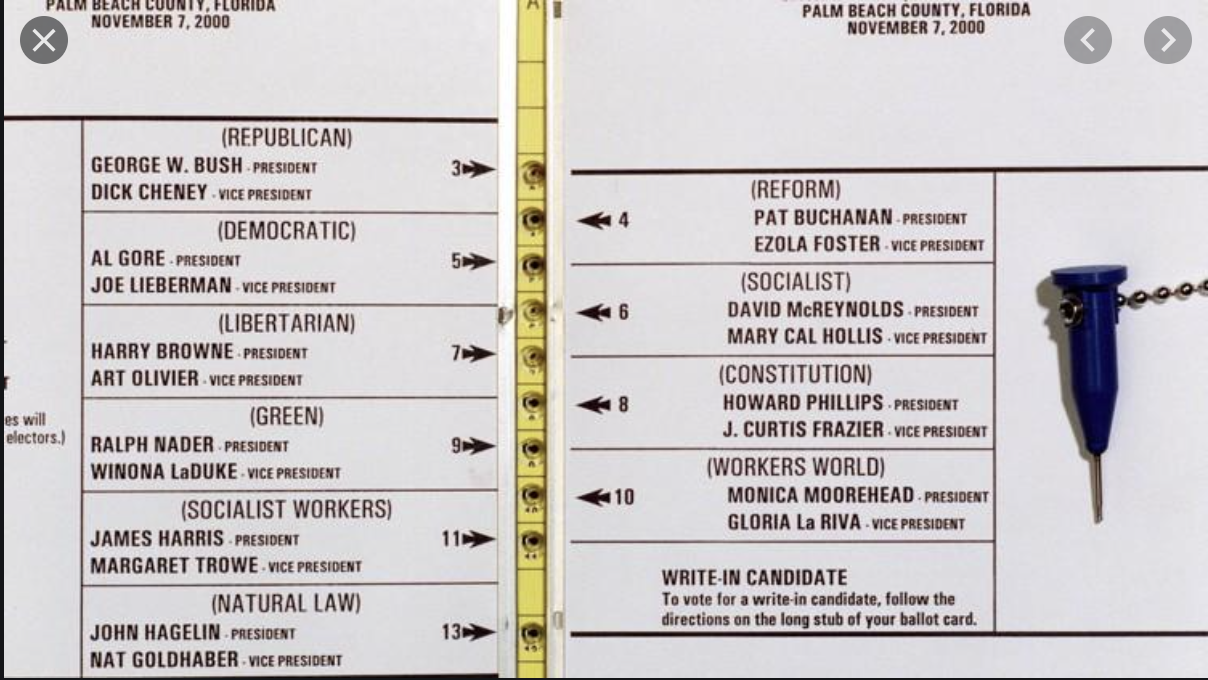
\includegraphics[width=0.9\linewidth]{images/09_palmballot} 

}

\caption{The Butterfly Ballot}\label{fig:butterfly}
\end{figure}

In the top left, you can see the first listed candidates are George W. Bush and Dick Cheney (the Republican Candidates). The next candidates (on the right) are actually Pat Buchanan and Ezola Foster (the Reform Party Candidates). However, if you are filling this in quickly, you can see how someone might accidentally think the second selection corresponds to Al Gore and Joe Lieberman.

If enough people made this mistake, this could actually have consequences for who wins the election. Remember, only 537 votes separated George W. Bush and Al Gore. To understand the scope of the problem, we are going to replicate analysis from Wand et al.~(2001)\citep{wand2001butterfly}, with much of the data and code coming from Kosuke Imai's Textbook: Quantitative Social Science: An Introduction.\citep{imai2018quantitative}.

Specifically, if voters are confused by the ballot, we would expect an unusually high number of votes for the Reform party candidates in Palm Beach. But how do we define ``an unusually high number of votes''. To operationalize this idea we will use the number of votes in a county for the Reform party in 1996 (the prior election) to predict how many votes a county will cast for the Reform party in 2000. If Palm Beach County has many more votes than predicted, then maybe the Butterfly ballot is the reason why.

To begin exploring this question, let's load up our data.

\begin{Shaded}
\begin{Highlighting}[]
\NormalTok{florida }\OtherTok{\textless{}{-}} \FunctionTok{read\_csv}\NormalTok{(}\StringTok{"florida.csv"}\NormalTok{)}
\CommentTok{\#\textgreater{} Rows: 67 Columns: 7}
\CommentTok{\#\textgreater{} {-}{-} Column specification {-}{-}{-}{-}{-}{-}{-}{-}{-}{-}{-}{-}{-}{-}{-}{-}{-}{-}{-}{-}{-}{-}{-}{-}{-}{-}{-}{-}{-}{-}{-}{-}{-}{-}{-}{-}}
\CommentTok{\#\textgreater{} Delimiter: ","}
\CommentTok{\#\textgreater{} chr (1): county}
\CommentTok{\#\textgreater{} dbl (6): Clinton96, Dole96, Perot96, Bush00, Gore00, Buc...}
\CommentTok{\#\textgreater{} }
\CommentTok{\#\textgreater{} i Use \textasciigrave{}spec()\textasciigrave{} to retrieve the full column specification for this data.}
\CommentTok{\#\textgreater{} i Specify the column types or set \textasciigrave{}show\_col\_types = FALSE\textasciigrave{} to quiet this message.}
\FunctionTok{head}\NormalTok{(florida)}
\CommentTok{\#\textgreater{} \# A tibble: 6 x 7}
\CommentTok{\#\textgreater{}   county   Clinton96 Dole96 Perot96 Bush00 Gore00 Buchanan00}
\CommentTok{\#\textgreater{}   \textless{}chr\textgreater{}        \textless{}dbl\textgreater{}  \textless{}dbl\textgreater{}   \textless{}dbl\textgreater{}  \textless{}dbl\textgreater{}  \textless{}dbl\textgreater{}      \textless{}dbl\textgreater{}}
\CommentTok{\#\textgreater{} 1 Alachua      40144  25303    8072  34124  47365        263}
\CommentTok{\#\textgreater{} 2 Baker         2273   3684     667   5610   2392         73}
\CommentTok{\#\textgreater{} 3 Bay          17020  28290    5922  38637  18850        248}
\CommentTok{\#\textgreater{} 4 Bradford      3356   4038     819   5414   3075         65}
\CommentTok{\#\textgreater{} 5 Brevard      80416  87980   25249 115185  97318        570}
\CommentTok{\#\textgreater{} 6 Broward     320736 142834   38964 177323 386561        788}
\end{Highlighting}
\end{Shaded}

Each row of the data is a county in Florida. In each row, we have counts for different presidential candidates in both 1996 and 2000. For example, in 1996, 40,144 votes were cast in Alachua county for Bill Clinton. 25,303 were cast for Bob Dole.

Our eventual goal will be to use the votes cast for Ross Perot (the Reform Party Candidate) in 1996, to predict how many votes a county will cast for Pat Buchanan in 2000 (the Reform Party Candidate).

The logic behind this design is that we might think counties are relatively consistent in their voting patterns. Maybe Palm Beach County is a county that happens to heavily support the Reform Party Candidates. If this is true, we should see high number of votes for Reform Party Candidates in both 1996 and 2000.

To begin our exploration, let's visualize the relationship between voting for Ross Perot in 1996 and Pat Buchanan in 2000. To do so we will construct a scatter plot with \texttt{Perot96} on the horizontal axis and \texttt{Buchanan00} on the vertical axis.

\begin{Shaded}
\begin{Highlighting}[]
\FunctionTok{ggplot}\NormalTok{(florida, }\AttributeTok{mapping=}\FunctionTok{aes}\NormalTok{(}\AttributeTok{x=}\NormalTok{Perot96, }\AttributeTok{y=}\NormalTok{Buchanan00)) }\SpecialCharTok{+} 
  \FunctionTok{geom\_point}\NormalTok{()}
\end{Highlighting}
\end{Shaded}

\begin{figure}

{\centering 
\includegraphics[width=0.8\linewidth]{09-week9_files/figure-latex/butter1-1} 

}

\caption{Relationship Between Buchanan and Perot Votes}\label{fig:butter1}
\end{figure}

We can see there is one point in the top right of this graph that seems to be a bit of an outlier. This county has much higher number of votes for Buchanan than any other county. In order to see which county this is, let's add the option \texttt{label=county} inside \texttt{aes()}. This will label each marker with the county it represents. To adjust the location and size of the marker, we will also specify \texttt{geom\_text(vjust=1.5,size=3)}.

\begin{Shaded}
\begin{Highlighting}[]
\FunctionTok{ggplot}\NormalTok{(florida, }
       \AttributeTok{mapping=}\FunctionTok{aes}\NormalTok{(}\AttributeTok{x=}\NormalTok{Perot96, }\AttributeTok{y=}\NormalTok{Buchanan00, }\AttributeTok{label=}\NormalTok{county)) }\SpecialCharTok{+} 
  \FunctionTok{geom\_point}\NormalTok{() }\SpecialCharTok{+} 
  \FunctionTok{geom\_text}\NormalTok{(}\AttributeTok{vjust=}\FloatTok{1.5}\NormalTok{, }\AttributeTok{size=}\DecValTok{3}\NormalTok{)}
\end{Highlighting}
\end{Shaded}

\begin{figure}

{\centering 
\includegraphics[width=0.8\linewidth]{09-week9_files/figure-latex/butter2-1} 

}

\caption{Relationship Between Buchanan and Perot Votes}\label{fig:butter2}
\end{figure}

We chose \texttt{(vjust=1.5,size=3)} to make the labels easily readable. You can play around with these parameters to see how it changes the appearance of the figure.

Now with the markers labeled we can see that Palm Beach is indeed the outlier county. But an important next question is how big of an outlier is Palm Beach? Is this enough to potentially change the outcome of the election? To answer this question concretely, we will first learn how to estimate a linear regression in R.

\section{Linear Regression}\label{linear-regression}

In this section we are going to review linear regression, and then estimate a linear regression which will help us understand whether the butterfly ballot impacted the 2000 U.S. Presidential Election. If you would like a more thorough review of linear regression, look back to Chapter 4 which includes a longer introduction to linear regression.

To review briefly, we can write a general linear regression equation as:

\[
Y_i = \beta_0 + \beta_1 \cdot X_i + \varepsilon_i
\]

Where \(Y_i\) is our dependent variable of interest, \(X_i\) is our independent variable of interest, \(\beta_0\) is the intercept, \(\beta_1\) is the slope coefficient and \(\varepsilon_i\) is the error term.

In our data, we choose estimates of \(\beta_0\) and \(\beta_1\), which we denote, \(\hat{\beta}_0\) and \(\hat{\beta}_1\), that minimize the sum of squared errors \(\sum_{i=1}^N(Y_i-\hat{Y}_i)^2\).

What do \(\hat{\beta}_0\) and \(\hat{\beta}_1\) tell us? Let's talk about \(\hat{\beta}_1\) first. This tells us how changes in \(X\) are associated with changes in \(Y\). If this value is positive, then increases in \(X\) are associated with increases in \(Y\). If it is negative, then increases in \(X\) are associated with decreases in \(Y\). The interpretation of \(\hat{\beta}_1\) is a 1-unit change in \(X\) is associated with a \(\hat{\beta}_1\)-unit change in \(Y\).

Once we have our estimates of the intercept and slope, we can also use them to form predictions. For example, the predicted value of \(Y\) for an individual with observable \(X_i=5\) is equal to:

\[
\hat{Y}_i = \hat{\beta}_0 + \hat{\beta}_1 \cdot 5 
\]
This is a good place to re-introduce our empirical application. Our goal is to use the number of votes for Perot in 1996 to predict the number of votes for Buchanan in 2000. One way to do this is to estimate a linear regression of the following form:

\[
Buchanan00_i = \beta_0 + \beta_1 \cdot Perot96_i + \varepsilon_i
\]

Once we estimate this regression equation, we can use the estimates to predict the number of Buchanan votes in Palm Beach County and compare to the actual number of votes in Palm Beach County. For example, hypothetically, if we predict Buchanan would receive 1000 votes in Palm Beach, but actually received 2000, then there would be 1000 more votes in Palm Beach than expected.

In R, the function we use to estimate linear regressions is the \texttt{lm()} function. The basic syntax of the command is:

\begin{Shaded}
\begin{Highlighting}[]
\NormalTok{lm.fit }\OtherTok{\textless{}{-}} \FunctionTok{lm}\NormalTok{(yvar }\SpecialCharTok{\textasciitilde{}}\NormalTok{ xvar, }\AttributeTok{data=}\NormalTok{df)}
\end{Highlighting}
\end{Shaded}

\begin{itemize}
\item
  \texttt{lm.fit} stores the estimates of the linear regression as an object in R.
\item
  \texttt{yvar} should be replaced with your \textbf{dependent variable}
\item
  \texttt{xvar} should be replaced with your \textbf{independent variable}
\item
  \texttt{df} should be the dataframe that is in your environment.
\end{itemize}

In our empirical application, the code below estimates a linear regression with \texttt{Buchanan00} as the dependent variable and \texttt{Perot96} as the independent variable:

\begin{Shaded}
\begin{Highlighting}[]
\NormalTok{lm.florida }\OtherTok{\textless{}{-}} \FunctionTok{lm}\NormalTok{(Buchanan00 }\SpecialCharTok{\textasciitilde{}}\NormalTok{ Perot96, }\AttributeTok{data=}\NormalTok{florida)}
\end{Highlighting}
\end{Shaded}

To view the basic estimates of the regression, we can type:

\begin{Shaded}
\begin{Highlighting}[]
\NormalTok{lm.florida}
\CommentTok{\#\textgreater{} }
\CommentTok{\#\textgreater{} Call:}
\CommentTok{\#\textgreater{} lm(formula = Buchanan00 \textasciitilde{} Perot96, data = florida)}
\CommentTok{\#\textgreater{} }
\CommentTok{\#\textgreater{} Coefficients:}
\CommentTok{\#\textgreater{} (Intercept)      Perot96  }
\CommentTok{\#\textgreater{}     1.34575      0.03592}
\end{Highlighting}
\end{Shaded}

So this displays our estimate of the intercept (\(\hat{\beta}_0=1.346\)) and slope coefficient (\(\hat{\beta}_1=0.036\)). The intercept tells us where the best fitted line intersects the vertical axis at \(X=0\). In terms of our example, the best fitted line is equal to 1.346 at \(Perot96_i=0\). Another way to interpret this is, hypothetically, if we had a county that cast zero votes for Perot in 1996, we would expect this county to cast 1.346 votes for Buchanan in 2000.

Now onto interpreting \(\hat{\beta}_1\): one additional vote for Perot in 1996 is associated with 0.035 more votes for Buchanan in 2000. You might be a little confused at the moment about why the slope coefficient seems so small. In the next section, we will discuss further how to interpret this regression, and in particular, how we can visualize its results. This will help us understand what our regression results imply in terms of figuring out whether something unusual is occurring in Palm Beach county.

\section{Plotting Regression Lines}\label{plotting-regression-lines}

In the prior section, we estimated

\[
Buchanan00_i = \beta_0 + \beta_1 \cdot Perot96_i + \varepsilon_i
\]
And found \(\hat{\beta}_0=1.346\) and \(\hat{\beta}_1=0.036\). These coefficients tells us the intercept and slope of the line that best fits our data. In this section we will show how to plot this best fit line in both base R and ggplot.

To begin, let's create a scatter plot with \texttt{Buchanan00} on the vertical axis and \texttt{Perot96} on the horizontal axis. We are also going to specify \texttt{pch=16} in this code to change the style of the markers. \texttt{pch} stands for plot character in R and can be used to change the shape or appearance of the points in a scatterplot.

\begin{Shaded}
\begin{Highlighting}[]
\FunctionTok{plot}\NormalTok{(florida}\SpecialCharTok{$}\NormalTok{Perot96, florida}\SpecialCharTok{$}\NormalTok{Buchanan00, }
     \AttributeTok{pch=}\DecValTok{16}\NormalTok{,}
     \AttributeTok{xlab=}\StringTok{"Votes for Perot in 1996"}\NormalTok{, }
     \AttributeTok{ylab=}\StringTok{"Votes for Buchanan in 2000"}\NormalTok{)}
\end{Highlighting}
\end{Shaded}

\begin{figure}

{\centering 
\includegraphics[width=0.8\linewidth]{09-week9_files/figure-latex/basescatter1-1} 

}

\caption{Relationship Between Buchanan and Perot Votes}\label{fig:basescatter1}
\end{figure}

Now our goal is to add the linear regression line to this plot. To do so, we will use the \texttt{abline()} function. \texttt{abline()} can be used to add lines to plots. If you pass the outcome of a linear regression to \texttt{abline()}, then the fitted line from that regression will be added to the plot. In other words, if we add \texttt{abline(lm.florida)}, then the best-fitted line from this regression will be added to the plot:

\begin{Shaded}
\begin{Highlighting}[]
\FunctionTok{plot}\NormalTok{(florida}\SpecialCharTok{$}\NormalTok{Perot96, florida}\SpecialCharTok{$}\NormalTok{Buchanan00, }
     \AttributeTok{pch=}\DecValTok{16}\NormalTok{,}
     \AttributeTok{xlab=}\StringTok{"Votes for Perot in 1996"}\NormalTok{, }
     \AttributeTok{ylab=}\StringTok{"Votes for Buchanan in 2000"}\NormalTok{)}
    \FunctionTok{abline}\NormalTok{(lm.florida)}
\end{Highlighting}
\end{Shaded}

\begin{figure}

{\centering 
\includegraphics[width=0.8\linewidth]{09-week9_files/figure-latex/basescatter2-1} 

}

\caption{Relationship Between Buchanan and Perot Votes}\label{fig:basescatter2}
\end{figure}

We can also customize the appearance of the line in a few ways. For example, \texttt{lty=2} will make the line dashed instead of solid. \texttt{lty} stands for line type and you can use a variety (see the help file for \texttt{plot} and search for \texttt{lty} to see the different options). \texttt{col="red"} will turn the line red.

\begin{Shaded}
\begin{Highlighting}[]
\FunctionTok{plot}\NormalTok{(florida}\SpecialCharTok{$}\NormalTok{Perot96, florida}\SpecialCharTok{$}\NormalTok{Buchanan00, }
     \AttributeTok{pch=}\DecValTok{16}\NormalTok{,}
     \AttributeTok{xlab=}\StringTok{"Votes for Perot in 1996"}\NormalTok{, }
     \AttributeTok{ylab=}\StringTok{"Votes for Buchanan in 2000"}\NormalTok{)}
    \FunctionTok{abline}\NormalTok{(lm.florida, }\AttributeTok{lty=}\DecValTok{2}\NormalTok{, }\AttributeTok{col=}\StringTok{"red"}\NormalTok{)}
\end{Highlighting}
\end{Shaded}

\begin{figure}

{\centering 
\includegraphics[width=0.8\linewidth]{09-week9_files/figure-latex/basescatter3-1} 

}

\caption{Relationship Between Buchanan and Perot Votes}\label{fig:basescatter3}
\end{figure}

Now let's learn how to plot the regression line in ggplot. In ggplot, the plot command can actually estimate the regression itself. In order to do so we will add to our plot the \texttt{geom\_smooth()} function. In general \texttt{geom\_smooth} adds fitted lines or curves to a plot. If we want a linear regression line, we can specify \texttt{geom\_smooth(method="lm")}. The option \texttt{lm} stands for linear model.

Further, we will want to specify \texttt{se=FALSE}. By default \texttt{geom\_smooth()} adds measures of uncertainty to our regression line, which we won't cover in this book. Lastly, we will use additional options to change the type and color of the line, as we did before. The full code to generate our scatter plot with a linear regression line appears below:

\begin{Shaded}
\begin{Highlighting}[]
\FunctionTok{ggplot}\NormalTok{(florida, }\AttributeTok{mapping=}\FunctionTok{aes}\NormalTok{(}\AttributeTok{x=}\NormalTok{Perot96, }\AttributeTok{y=}\NormalTok{Buchanan00)) }\SpecialCharTok{+} 
  \FunctionTok{geom\_point}\NormalTok{() }\SpecialCharTok{+} 
  \FunctionTok{xlab}\NormalTok{(}\StringTok{"Votes for Perot in 1996"}\NormalTok{) }\SpecialCharTok{+} 
  \FunctionTok{ylab}\NormalTok{(}\StringTok{"Votes for Buchanan in 2000"}\NormalTok{) }\SpecialCharTok{+} 
  \FunctionTok{geom\_smooth}\NormalTok{(}\AttributeTok{method=}\StringTok{"lm"}\NormalTok{, }\AttributeTok{se=}\ConstantTok{FALSE}\NormalTok{, }\AttributeTok{linetype=}\StringTok{"dashed"}\NormalTok{,}\AttributeTok{color=}\StringTok{"red"}\NormalTok{)}
\CommentTok{\#\textgreater{} \textasciigrave{}geom\_smooth()\textasciigrave{} using formula = \textquotesingle{}y \textasciitilde{} x\textquotesingle{}}
\end{Highlighting}
\end{Shaded}

\begin{figure}

{\centering 
\includegraphics[width=0.8\linewidth]{09-week9_files/figure-latex/geomscatter-1} 

}

\caption{Relationship Between Buchanan and Perot Votes}\label{fig:geomscatter}
\end{figure}

\section{Predicted Values and Residuals}\label{predicted-values-and-residuals}

Now that we have estimated and plotted our linear regression line, let's review how to form predicted values and residuals.

In general, the predicted value is given by:

\[
\hat{Y}_i = \hat{\beta}_0 + \hat{\beta}_1 \cdot X_i
\]

This gives us our best guess for a value of \(Y_i\) given a value of \(X_i\), based on the linear regression estimates. This is the best fit line we plotted in the prior section. We can use this equation to form predicted values. For example, imagine I tell you a Alachua county in 1996 cast 8,072 votes for Ross Perot. Based on this number and the linear regression, what do you expect to be the number of Pat Buchanan votes cast?

\[
\hat{Buchanan00_i}= 1.346 + 0.036 \cdot 8072 \approx 292
\]

In other words, we expect Alachua county to cast 292 votes for Pat Buchanan. Now, this is just a prediction. We are using a single variable (Ross Perot votes) to predict the number of Buchanan votes. In reality, the number of Buchanan votes likely depends on a variety of factors. Therefore, our model will have error associated with, which we refer to as the residual.

The residual is given by the difference between the actual value and the predicted value. For example, Alachua county cast 263 votes for Buchanan. The residual is therefore given by:

\[
\hat{residual}_i = Y_i - \hat{Y}_i=263-292 = -29
\]

Now, we could do this manually for every single observation, but it will be much easier to do this automatically in R. This will allow us to construct the residual for every county in the data. We are particularly interested in the residual for Palm Beach county. This residual will tell us how many more votes were cast in Palm Beach for Buchanan relative to what we would have expected based on the county's voting patterns for Perot.

To do so we will again estimate a linear regression with \texttt{Buchanan00} as the dependent variable and \texttt{Perot96} as the independent variable.

\begin{Shaded}
\begin{Highlighting}[]
\NormalTok{lm.florida }\OtherTok{\textless{}{-}} \FunctionTok{lm}\NormalTok{(Buchanan00 }\SpecialCharTok{\textasciitilde{}}\NormalTok{ Perot96, }\AttributeTok{data=}\NormalTok{florida)}
\end{Highlighting}
\end{Shaded}

\texttt{lm.florida} is known as a list object. It contains a lot of information from our linear regression. We can use the \texttt{names()} function to figure out what \texttt{lm.florida} contains:

\begin{Shaded}
\begin{Highlighting}[]
\FunctionTok{names}\NormalTok{(lm.florida)}
\CommentTok{\#\textgreater{}  [1] "coefficients"  "residuals"     "effects"      }
\CommentTok{\#\textgreater{}  [4] "rank"          "fitted.values" "assign"       }
\CommentTok{\#\textgreater{}  [7] "qr"            "df.residual"   "xlevels"      }
\CommentTok{\#\textgreater{} [10] "call"          "terms"         "model"}
\end{Highlighting}
\end{Shaded}

So many of the information stored here we won't use in this course. But there are two elements that will be useful for us. You can see one of the names is \texttt{fitted.values} and another is \texttt{residual}. Fitted values is another name for predicted values.

We can extract the information from \texttt{lm.florida} by using the dollar sign operator. For example, if we want to add a new variable to the dataset that is the fitted value for each observation, we type:

\begin{Shaded}
\begin{Highlighting}[]
\NormalTok{florida}\SpecialCharTok{$}\NormalTok{predBuchanan00 }\OtherTok{\textless{}{-}}\NormalTok{ lm.florida}\SpecialCharTok{$}\NormalTok{fitted.values}
\end{Highlighting}
\end{Shaded}

\texttt{predBuchanan00} is the name of the new variable and it is equal to the fitted values from the regression estimation. We can similarly extract the residual from our \texttt{lm.florida} object and add to the data frame \texttt{florida}.

\begin{Shaded}
\begin{Highlighting}[]
\NormalTok{florida}\SpecialCharTok{$}\NormalTok{residuals }\OtherTok{\textless{}{-}}\NormalTok{ lm.florida}\SpecialCharTok{$}\NormalTok{residuals}
\end{Highlighting}
\end{Shaded}

Now, let's look at the data to try and understand our process so far.

\begin{verbatim}
#> # A tibble: 67 x 4
#>    county    Buchanan00 predBuchanan00 residuals
#>    <chr>          <dbl>          <dbl>     <dbl>
#>  1 Alachua          263          291.     -28.3 
#>  2 Baker             73           25.3     47.7 
#>  3 Bay              248          214.      34.0 
#>  4 Bradford          65           30.8     34.2 
#>  5 Brevard          570          908.    -338.  
#>  6 Broward          788         1401.    -613.  
#>  7 Calhoun           90           24.0     66.0 
#>  8 Charlotte        182          281.     -98.9 
#>  9 Citrus           270          262.       8.49
#> 10 Clay             186          119.      66.8 
#> # i 57 more rows
\end{verbatim}

So for Alachua county the number of Buchanan votes in 2000 was 263. The predicted Buchanan votes was 291.251 (if you view your data frame you will be able to see more decimal places). Therefore the residual is -28.3. The reason this is slightly different than what we had above is because when we formed this manually we rounded the coefficients in the regression. When R does the computation, it is much more precise than we were, which explains why predicted values and residuals are slightly different than the manual computation.

Now let's order the dataset by the magnitude of the residual. Observations with large residuals will be those in which our predictions are very different than our predicted value. To sort data based on the value of a variable, we can use the \texttt{arrange()} function.

For our purposes we want to sort based on the absolute value of the residual. Therefore, we will specify \texttt{arrange(abs(residuals))}. The \texttt{abs()} function takes the absolute value of a number. However, in addition, we want the largest residuals to be at the top. By default, \texttt{arrange} sorts the data from lowest to highest. To change this, we can ask for the data to be presented in descending order, by specifying \texttt{arrange(desc(abs(residuals)))}. The \texttt{desc()} function specifies to order the data in descending order (from largest to smallest).

Additionally, we can combine \texttt{arrange} with other functions using the pipe operator. In this example, we are really only interested in a few variables at the moment. So let's first select those variables, and then display the data from largest residual (in absolute value) to lowest residual.

\begin{Shaded}
\begin{Highlighting}[]
\NormalTok{florida }\SpecialCharTok{\%\textgreater{}\%} 
  \FunctionTok{select}\NormalTok{(county,Buchanan00,predBuchanan00,residuals) }\SpecialCharTok{\%\textgreater{}\%}
  \FunctionTok{arrange}\NormalTok{(}\FunctionTok{desc}\NormalTok{(}\FunctionTok{abs}\NormalTok{(residuals)))}
\end{Highlighting}
\end{Shaded}

\begin{verbatim}
#> # A tibble: 67 x 4
#>    county     Buchanan00 predBuchanan00 residuals
#>    <chr>           <dbl>          <dbl>     <dbl>
#>  1 PalmBeach        3407          1105.     2302.
#>  2 Broward           788          1401.     -613.
#>  3 Lee               305           662.     -357.
#>  4 Brevard           570           908.     -338.
#>  5 Miami-Dade        560           889.     -329.
#>  6 Pinellas         1013          1330.     -317.
#>  7 Sarasota          305           538.     -233.
#>  8 Orange            446           655.     -209.
#>  9 Escambia          502           310.      192.
#> 10 St.Lucie          124           306.     -182.
#> # i 57 more rows
\end{verbatim}

So Palm Beach county cast 3407 votes for Buchanan. Based on the linear regression, we would have expected 1105 votes for Buchanan. Therefore, there were 2302 more votes than expected.

Now recall the George Bush won Florida by 537 votes. Now, if the excess votes in Palm Beach were driven by the design of the butterfly ballots, then we are seeing this excess voting for Buchanan because individuals were confused about the design and were accidentally selecting Buchanan instead of Gore.

If this is true, then Al Gore would have actually received approximately 2,000 more votes. This would have been enough to make him the winner in Florida, and given the closeness of the election, the winner overall. In other words, using some simple data analysis techniques, we've found convincing evidence that a poorly designed ballot in a single Florida county was enough to flip the 2000 presidential election!

\section{Get Out to Vote Experiments}\label{get-out-to-vote-experiments}

Next, we are going to shift gears to another voting application. One notorious issue in politics is getting people to vote. In particular, it is extremely difficult to get voters to turn out to vote in primary elections, even though primary elections are incredibly important. They select the candidates who will run in the general election. Yet, year after year, voter turnout for these primary elections is pretty low. For example, in California, voter turnout in general elections between 2000-2012 was about 65.5 percent among registered voters. In contrast, voter turnout in primary elections during this period was around 40.8 percent.

One reason for lack of voting may be due to a lack of mobilization. Maybe some simple information and encouragement to voting in primaries will incentivize individuals to vote. In Hill and Kousser (2016)\citep{hill2016turning}, the authors test this idea by implementing a large-scale experiment in the 2014 congressional primary elections in California.

In their study, Hill and Kousser were particularly interested in targeting those individuals who vote in general elections, but not in primaries. These are perhaps the individuals for which a treatment will be most successful. They are engaged in politics on big occasions (general elections), but not engaged in other occasions (primary elections).

To be specific, Hill and Kousser sent three types of letters to individuals in advance of the 2014 primary election

\begin{itemize}
\tightlist
\item
  Letter 1: Basic information about the election
\item
  Letter 2: Basic information plus information about California top two primaries
\item
  Letter 3: Basic information plus information about turnout for the respondent's party
\end{itemize}

The letters were aimed at testing different reasons why people may or may not vote. Letter 1 tests whether basic information about when the election is occurring helps promote turnout. Letter 2 is aimed to providing information about one particularly confusing element of Congressional campaigns in California. In 2012, a law in California was passed that made it a ``top-two'' primary state. This means that any individual in California can vote for any candidate in a primary, regardless of party affiliation. The top two candidates with the most votes then continue to the general election in November. Under this system it is possible that the top two candidates come from the same party. Hill and Kousser wanted to test whether lack of understanding about the new system prevented some from voting.

The last letter also included information about voter turnout among the respondents party. The authors hypothesize that seeing low voter turnout among your party may be especially effective in incentivizing an individual to vote. In other words, individuals registered as Republican were provided the Republican voter turnout in the prior election, while individuals registered as Democrats were provided the voter turnout for Democrats in the prior election.

One impressive aspect of this experiment is its scale. In total, Hill and Kousser (2016) sent around 150,000 letters to Californians before the election. This will allow us to get very precise answers to how informational interventions impact voter turnout. Additionally, given voting records are public data, we also have a very large control group in this experiment: individuals who did not receive one of the three letters.

\section{Regression (Binary Variables)}\label{regression-binary-variables}

To study the impacts of receiving a mailer on voter turnout, we are again going to turn to linear regression. For our purposes, we will study the impact of receiving any mailer. Therefore, conceptually, you should think of individuals who received any letter as the treatment group, and individuals who did not receive a letter as the control group. To estimate the impact of receiving a mailer we will estimate a linear regression of the following form:

\[
Y_i = \beta_0 + \beta_1 \cdot X_i + \varepsilon_i
\]

Where \(Y_i\) is equal to 1 if the individual voted and zero otherwise, and \(X_i\) is equal to one if the individual received a mailer and zero otherwise. This is a bit different than most of examples so far, because in this example both \(Y_i\) and \(X_i\) are binary, meaning they take on only two values.

What is the interpretation of \(\beta_1\) in this example. Our general rule is: when \(X_i\) increases by 1, this is associated with a \(\beta_1\)-unit change in \(Y_i\). Because \(X_i=0\) if in the control and 1 if in the treatment, a 1-unit increase in \(X_i\) is going from control to treatment. In other words, moving an individual from the control to receiving a letter is associated with a \(\beta_1\) unit change in \(Y_i\). But \(Y_i\) is also binary. So imagine for a moment \(\beta_1=0.01\). What does a \(0.01\) change in \(Y_i\) imply? Well, this is a \(\beta_1 \cdot 100=0.01 \cdot 100 = 1\) percentage point increase in \(Y_i\).

Another way to think through this interpretation is through predicted values. Imagine now \(\beta_0=0.5\) and \(\beta_1=0.01\). Next, I ask what is the predicted value of \(Y_i\) for an individual in the control (i.e.~\(X_i=0\)):

\[
\hat{Y}_i = \beta_0 + \beta_1 \cdot X_i = 0.5 + 0.01 \cdot 0 = 0.50
\]

In simpler terms, we expect 50 percent of individuals in the control to vote. Recall that when you take the average of a binary variable that takes on values of zero or one, this average is equal to the fraction of individuals with a 1. Therefore, in this case, a value of 0.5 indicates half the individuals have a value of \(Y_i=1\). Put even more simply, half of all individuals voted. Next, I ask what is the predicted value of \(Y_i\) for an individual in the treatment:

\[
\hat{Y}_i = \beta_0 + \beta_1 \cdot X_i = 0.5 + 0.01 \cdot 1 = 0.51
\]
Therefore, we expect 51 percent of individuals to vote in the treatment. Therefore, the impact of going to control to treatment is a 1 percentage point increase in the probability of voting. If you need a review on the difference between percent and percentage point, check out Chapter 1.8. Specifically, it would \textbf{not} be correct here to say that treatment increases voting rates by 1 percent. Now that we understand the interpretation of linear regression with binary variables, let's go implement this regression in R to assess how receiving a mailer impacted voter turnout.

The data for this application comes from a csv file named \texttt{turnout.csv}. Let's load this into R as a tibble.

\begin{Shaded}
\begin{Highlighting}[]
\NormalTok{turnout }\OtherTok{\textless{}{-}} \FunctionTok{read\_csv}\NormalTok{(}\StringTok{"turnout.csv"}\NormalTok{)}
\CommentTok{\#\textgreater{} Rows: 3872268 Columns: 5}
\CommentTok{\#\textgreater{} {-}{-} Column specification {-}{-}{-}{-}{-}{-}{-}{-}{-}{-}{-}{-}{-}{-}{-}{-}{-}{-}{-}{-}{-}{-}{-}{-}{-}{-}{-}{-}{-}{-}{-}{-}{-}{-}{-}{-}}
\CommentTok{\#\textgreater{} Delimiter: ","}
\CommentTok{\#\textgreater{} chr (2): Party, treatment.assign}
\CommentTok{\#\textgreater{} dbl (3): LocalityCode, yvar, mailer}
\CommentTok{\#\textgreater{} }
\CommentTok{\#\textgreater{} i Use \textasciigrave{}spec()\textasciigrave{} to retrieve the full column specification for this data.}
\CommentTok{\#\textgreater{} i Specify the column types or set \textasciigrave{}show\_col\_types = FALSE\textasciigrave{} to quiet this message.}
\end{Highlighting}
\end{Shaded}

This is a very large dataset. The data includes information on over 3.8 million individuals in California. Let's take a look at a small slice of the data:

\begin{verbatim}
#> # A tibble: 3,872,268 x 5
#>    LocalityCode Party  yvar treatment.assign mailer
#>           <dbl> <chr> <dbl> <chr>             <dbl>
#>  1            1 REP       0 Control               0
#>  2            1 NPP       0 Control               0
#>  3            1 DEM       1 Control               0
#>  4            1 REP       0 Control               0
#>  5            1 DEM       0 Control               0
#>  6            1 NPP       0 Control               0
#>  7            1 DEM       0 Control               0
#>  8            1 DEM       0 Control               0
#>  9            1 REP       0 Control               0
#> 10            1 NPP       0 Control               0
#> # i 3,872,258 more rows
\end{verbatim}

The first variable \texttt{LocalityCode} indicates the county the individual is voting in. \texttt{Party} is the registered party of the individual. \texttt{yvar} is our main dependent variable. This variable is equal to 1 if the individual voted in the 2014 primary election and zero if the individual did not vote. \texttt{treatment.assign} indicates whether this individual is in the control group (i.e.~did not receive a letter) or one of the treatment arms. The last variable \texttt{mailer} is equal to 1 if the individual received any mailer, and zero if the individual is in the control group.

For our application, we want to test whether receiving a mailer impacts the probability an individual votes. Therefore, we will regress the variable \texttt{yvar} on the variable \texttt{mailer}. Just as before, we need to save our estimates as a new object.

\begin{Shaded}
\begin{Highlighting}[]
\NormalTok{lm.turnout }\OtherTok{\textless{}{-}} \FunctionTok{lm}\NormalTok{(yvar }\SpecialCharTok{\textasciitilde{}}\NormalTok{ mailer, }\AttributeTok{data=}\NormalTok{turnout)}
\end{Highlighting}
\end{Shaded}

Now let's look at the results:

\begin{Shaded}
\begin{Highlighting}[]
\NormalTok{lm.turnout}
\CommentTok{\#\textgreater{} }
\CommentTok{\#\textgreater{} Call:}
\CommentTok{\#\textgreater{} lm(formula = yvar \textasciitilde{} mailer, data = turnout)}
\CommentTok{\#\textgreater{} }
\CommentTok{\#\textgreater{} Coefficients:}
\CommentTok{\#\textgreater{} (Intercept)       mailer  }
\CommentTok{\#\textgreater{}    0.093125     0.004899}
\end{Highlighting}
\end{Shaded}

So let's interpret this regression. To do so, let's compute what the regression predicts regarding voting for an individual in the control:

\[
\hat{Y}_i = 0.093 + 0.005 \cdot 0 = 0.093
\]

In simple terms, 9.3 percent of individuals in the control group voted in the election. For individuals in the treatment, we get:

\[
\hat{Y}_i = 0.093 + 0.005 \cdot 1 = 0.093+ 0.005 = 0.098
\]

Therefore, in the treatment group, about 9.8 percent of individuals turned out to vote. Therefore, our treatment is expected to increase voting rates by 0.5 percentage points.

\section{Conclusion}\label{conclusion-7}

In this chapter, we have introduced two voting examples. In the first application, we showed that a poorly designed ballot may have changed the 2000 U.S. Presidential election. In the second, we showed that a massive campaign that sent mailers to over 150,000 Californians increased voter turnout in primary elections.
In both of these applications, we used regression to analyze the data. In our first application, regression gave us a way to form predictions. In particular, we needed to form a prediction for Palm Beach County regarding how many votes Pat Buchanan (the Reform Party Candidate) would receive. This was important because after the election, individuals claimed that the ballot was confusing, and led people to mistakenly vote for Pat Buchanan rather than Al Gore (check out Figure \ref{fig:butterfly} to see if you agree).

However, we still needed a way in the data to see whether it appears that ``too many'' individuals voted for Pat Buchanan. To do this, we predicted county-level votes for Pat Buchanan using the number of votes cast for Ross Perot in 1996. This is likely a good predictor because Ross Perot and Pat Buchanan were both from the same party (the Reform Party).

Using the regression estimates, we predicted that Palm Beach county would cast 1105 votes for Buchanan. In actuality, Palm Beach cast 3407 votes for Buchanan. In other words, Palm Beach had over 2000 more votes for Buchanan than expected. This discrepancy is large enough to potentially swing the election. George Bush won Florida by only 537 votes. Had those 2000 votes for Buchanan been cast for Al Gore, then Al Gore would have won Florida and the election overall.

In the second application, we used regression to estimate a treatment effect: the effect of receiving a mailer on voter turnout. It is notoriously difficult to get individuals to vote in primary elections. In Hill and Kousser (2016), the authors sent an astounding 150,000 letters to Californians, providing them with different forms of information about the election. The scope of the project allowed the authors to detect even small changes in voting behavior. In the end, they found the mailer increased voting by about 0.5 percentage points. This may seem small, but if applied to the population of California, this implies thousands of additional voters.

\section*{Function Descriptions}\label{function-descriptions-3}
\addcontentsline{toc}{section}{Function Descriptions}

\textbf{Functions Used}

\begin{itemize}
\item
  \texttt{lm} -- Estimates linear regression in R. General syntax is given by \texttt{lm.fit\ \textless{}-\ lm(yvar\ \textasciitilde{}\ xvar,\ data=df)}. \texttt{lm.fit} is an object that is created and contains results of the linear regression.

  \begin{itemize}
  \tightlist
  \item
    \texttt{lm} stores many important results from linear regression, including \texttt{coefficients}, \texttt{fitted.values}, and \texttt{residuals}. To extract an element type \texttt{lm.fit\$coefficients}.
  \end{itemize}
\item
  \texttt{abline} -- adds linear regression line to plots in Base R.
\item
  \texttt{geom\_smooth(method="lm",se=FALSE)} -- adds linear regression line to plots in ggplot2.
\end{itemize}

\chapter{Unconditional Cash Transfers}\label{unconditional-cash-transfers}

\section{Motivation}\label{motivation}

A central goal of development economics is to understand ways to alleviate global poverty. However, the exact design of policies is often up for debate.

For example, imagine you are a charity or government that has funds to disburse to individuals in poverty. How would you go about doing this? One response is to make the transfers conditional. In other words, you give individuals cash to purchase particular items. For example, many programs allocate funds to be used for food or education.

Another way to disburse these funds is to do so unconditionally. This gives individuals the autonomy to decide for themselves what they would like to spend the money on. This week, we will use data from Haushofer and Shapiro (2016)\citep{haushofer2016short}, which studies the impact of unconditional cash transfers in Kenya on the economic and psychological well-being of recipients. This study was made possible due to the charitable organization, Give Directly, a charity co-founded by Paul Niehaus, professor of Economics at UC San Diego.

In particular, Haushofer and Shapiro randomize a couple of aspects including (1) whether a household receives an unconditional cash transfer and (2) the timing of the transfer (monthly vs.~lump sum) and (3) the size of the transfer (small \$400 or large \$1500). A key strength of the study is that they can also study a wide range of outcomes, including assets, expenditures, food security, health, education expenditures, and psychological well being.

We will only be able to explore a fraction of all of these outcomes, and for this exercise we will focus on total assets. You can interpret assets as the amount of savings an individual has at a particular point in time. To get started, let's head over to R to load up the data.

\section{The Data}\label{the-data}

The data from this experiment is provided in the \texttt{uct.csv} file. First, we are again going to load \texttt{tidyverse}.

\begin{Shaded}
\begin{Highlighting}[]
\FunctionTok{library}\NormalTok{(tidyverse)}
\end{Highlighting}
\end{Shaded}

Now let's read in the \texttt{uct.csv} file:

\begin{Shaded}
\begin{Highlighting}[]
\NormalTok{uct }\OtherTok{\textless{}{-}} \FunctionTok{read\_csv}\NormalTok{(}\StringTok{"uct.csv"}\NormalTok{)}
\NormalTok{Rows}\SpecialCharTok{:} \DecValTok{940}\NormalTok{ Columns}\SpecialCharTok{:} \DecValTok{19}
\SpecialCharTok{{-}{-}}\NormalTok{ Column specification }\SpecialCharTok{{-}{-}{-}{-}{-}{-}{-}{-}{-}{-}{-}{-}{-}{-}{-}{-}{-}{-}{-}{-}{-}{-}{-}{-}{-}{-}{-}{-}{-}{-}{-}{-}{-}{-}{-}{-}}
\NormalTok{Delimiter}\SpecialCharTok{:} \StringTok{","}
\FunctionTok{dbl}\NormalTok{ (}\DecValTok{19}\NormalTok{)}\SpecialCharTok{:}\NormalTok{ treat, village, treatXfemalerec, asset\_after, ...}

\NormalTok{i Use }\StringTok{\textasciigrave{}}\AttributeTok{spec()}\StringTok{\textasciigrave{}}\NormalTok{ to retrieve the full column specification }\ControlFlowTok{for}\NormalTok{ this data.}
\NormalTok{i Specify the column types or set }\StringTok{\textasciigrave{}}\AttributeTok{show\_col\_types = FALSE}\StringTok{\textasciigrave{}}\NormalTok{ to quiet this message.}
\end{Highlighting}
\end{Shaded}

So we have 940 observations and 19 columns (i.e.~variables). The first variable \texttt{treat} in is equal to 1 if the individual is in the treated group (received some cash payment) and zero of the individual is in the control group (did not receive a cash payment). Two variables we will be particularly interested in are \texttt{asset\_before} and \texttt{asset\_after}. In order to understand the impact of the cash transfer, we will compare the changes in assets for the treated workers relative to the change in assets for the control group.

Although we will focus on assets, as mentioned previously, there are a wide range of variables in the data. For each variable, we have a measurement both before and after the cash payments were made. Given the range of variables in the data, this will allow for a comprehensive study of how individuals outcomes are impacted by cash transfers.

In the last columns, we also have information about the exact treatment. For example, the variable \texttt{treatXlarge} is equal to 1 if the individual is in the treatment group and the individual received a large cash transfer (\$1500). The variable \texttt{treatXmonthlyXsmall} is equal to 1 if the individual is in the treatment group which received small monthly payments. Although we will not study the impact by each particular treatment, the design of the experiment also allows the authors understand how the size and timing of payments impacts overall welfare.

Next, we will start analyzing the data. However, to do so, we will introduce a new concept: user-written functions. So far, every function we have used has either come from base R or from a package we have loaded. In the next section, we will learn how to write our own functions.

\section{Functions (Part 1)}\label{functions-part-1}

To clarify how to write your own functions, let's first review what a function is. A function takes an input, performs some operations on this input, and then provides an output. For example, for the \texttt{mean()} function in R, the input will be a vector of numbers, and the output is the mean of the vector.

In data analysis, we often find ourselves repeating the same process over and over. Functions can help in these situations. If you find yourself repeating the same analysis over and over by copying and pasting code, but just changing small elements, then it might be time to put this analysis into a function.

This is precisely why R has provided the \texttt{mean()} function. We calculate means all the times. Therefore, it makes sense to have a function that will quickly compute the mean. But what if our analysis is more complicated? What if there is no standard function that performs it? In that case, we can write our own function.

So how do we go about creating a function in R. There are basically four things we need to decide. First, what will the function name be? Similar to choosing variable names, we want something relatively simple, but also descriptive. Second, what will be the inputs? For the \texttt{mean()} function the input is a list of numbers. But inputs can be anything: a vector, a character, a dataframe. Lastly, we decide on what the function does to the input to create the output.

Let's first introduce the general syntax, before writing our own simple function:

\begin{Shaded}
\begin{Highlighting}[]
\NormalTok{functionname }\OtherTok{\textless{}{-}} \ControlFlowTok{function}\NormalTok{(input) \{}
  
\NormalTok{  Perform operations to produce output }
  
  \FunctionTok{return}\NormalTok{(output)}
  
\NormalTok{\}}
\end{Highlighting}
\end{Shaded}

This can be a little abstract, so let's do an example with inputs, operations, and outputs that we understand. Let's manually create our own mean function.

\begin{Shaded}
\begin{Highlighting}[]
\NormalTok{mymean }\OtherTok{\textless{}{-}}\ControlFlowTok{function}\NormalTok{(num) \{}
  
\NormalTok{  output }\OtherTok{\textless{}{-}} \FunctionTok{sum}\NormalTok{(num)}\SpecialCharTok{/}\FunctionTok{length}\NormalTok{(num)}
  
  \FunctionTok{return}\NormalTok{(output)}
  
\NormalTok{\}}
\end{Highlighting}
\end{Shaded}

The name of this function is \texttt{mymean}. Therefore, when I want to use it I can specify \texttt{mymean()}. The input is named \texttt{num}. The input is going to be a list of numbers. What does the function do to a list of numbers. It adds them up \texttt{sum(num)} and then divides by the number of elements in the list of numbers. For example, imagine my list of numbers is 3, 5 and 7. Then \texttt{sum(num)=3+5+7=15} and \texttt{length(num)=3}, implying \texttt{output\textless{}-5}. The last line tells R to return this number as the output. Note that all of the code that create the output is within curly brackets. The curly brackets tell R when the function starts and when it ends.

We can actually see how this works by creating this vector in R.

\begin{Shaded}
\begin{Highlighting}[]
\NormalTok{myvec }\OtherTok{\textless{}{-}} \FunctionTok{c}\NormalTok{(}\DecValTok{3}\NormalTok{,}\DecValTok{5}\NormalTok{,}\DecValTok{7}\NormalTok{)}
\end{Highlighting}
\end{Shaded}

Now let's apply our function \texttt{mymean()} to the vector \texttt{myvec}.

\begin{Shaded}
\begin{Highlighting}[]
\FunctionTok{mymean}\NormalTok{(myvec)}
\NormalTok{[}\DecValTok{1}\NormalTok{] }\DecValTok{5}
\end{Highlighting}
\end{Shaded}

Now that we understand the basics of creating our own function, let's create a function for our empirical application this week which studies the impact of unconditional cash transfers in Kenya.

Our goal is to compare assets between the treated and control households. Of course, we can do this without creating a function, we just need to take the mean of \texttt{asset\_after} conditional on \texttt{treat==1} and then compare to the mean of \texttt{asset\_after} conditional on \texttt{treat==0}.

\begin{Shaded}
\begin{Highlighting}[]
\FunctionTok{mean}\NormalTok{(uct}\SpecialCharTok{$}\NormalTok{asset\_after[uct}\SpecialCharTok{$}\NormalTok{treat}\SpecialCharTok{==}\DecValTok{1}\NormalTok{])}
\NormalTok{[}\DecValTok{1}\NormalTok{] }\FloatTok{790.9253}
\end{Highlighting}
\end{Shaded}

So in the treatment group, on average, individuals have 791 dollars in assets after receiving the cash transfer. These measurements were taken 9 months after the treatment.

\begin{Shaded}
\begin{Highlighting}[]
\FunctionTok{mean}\NormalTok{(uct}\SpecialCharTok{$}\NormalTok{asset\_after[uct}\SpecialCharTok{$}\NormalTok{treat}\SpecialCharTok{==}\DecValTok{0}\NormalTok{])}
\NormalTok{[}\DecValTok{1}\NormalTok{] }\FloatTok{494.8041}
\end{Highlighting}
\end{Shaded}

So in the control group, on average, individuals have 495 dollars in assets. What this result tells us is that 9 months after the program began, treated individuals still have higher savings than control individuals. This indicates that individuals do not immediately consume the transfer payment, but instead save some of it for the future.

One thing to notice is that the two lines of code we wrote to perform this analysis vary by a single number. In the first, we set \texttt{treat==1} and the second we set \texttt{treat==0}. If you find yourself writing the same code multiple times, but just changing a single element or two, this might be a good time to write a function.

We will now write a function that varies this one input: the treatment value. Then, depending on whatever treatment value you pass to the function, the function will compute the mean for individuals with that treatment value. Let's name our function \texttt{treatment} and have the input be \texttt{treatvalue}.

\begin{Shaded}
\begin{Highlighting}[]
\NormalTok{treatmean }\OtherTok{\textless{}{-}} \ControlFlowTok{function}\NormalTok{(treatvalue)\{}
  
\NormalTok{  output }\OtherTok{\textless{}{-}} \FunctionTok{mean}\NormalTok{(uct}\SpecialCharTok{$}\NormalTok{asset\_after[uct}\SpecialCharTok{$}\NormalTok{treat}\SpecialCharTok{==}\NormalTok{treatvalue])}
  
  \FunctionTok{return}\NormalTok{(output)}

\NormalTok{\}}
\end{Highlighting}
\end{Shaded}

So this function is allowing the user to pass in a \texttt{treatvalue}, which in this case will be either zero or 1. Then, based on this \texttt{treatvalue} the function will calculate mean assets after for individuals with that \texttt{treatvalue}. For example, if we want to calculate the mean assets after for the treatment group we can type:

\begin{Shaded}
\begin{Highlighting}[]
\FunctionTok{treatmean}\NormalTok{(}\DecValTok{1}\NormalTok{)}
\NormalTok{[}\DecValTok{1}\NormalTok{] }\FloatTok{790.9253}
\end{Highlighting}
\end{Shaded}

If we want to calculate the mean assets after for the control group, we type:

\begin{Shaded}
\begin{Highlighting}[]
\FunctionTok{treatmean}\NormalTok{(}\DecValTok{0}\NormalTok{)}
\NormalTok{[}\DecValTok{1}\NormalTok{] }\FloatTok{494.8041}
\end{Highlighting}
\end{Shaded}

Now, there are often many different ways to code the same function. For example, imagine instead of using base R, we want to calculate this using the tidyverse.

\begin{Shaded}
\begin{Highlighting}[]
\NormalTok{treatmean }\OtherTok{\textless{}{-}} \ControlFlowTok{function}\NormalTok{(treatvalue)\{}
\NormalTok{  output }\OtherTok{\textless{}{-}}\NormalTok{ uct }\SpecialCharTok{\%\textgreater{}\%}
    \FunctionTok{filter}\NormalTok{(treat}\SpecialCharTok{==}\NormalTok{treatvalue) }\SpecialCharTok{\%\textgreater{}\%}
    \FunctionTok{summarize}\NormalTok{(}\AttributeTok{assetmean=}\FunctionTok{mean}\NormalTok{(asset\_after))}
  \FunctionTok{return}\NormalTok{(output)}
\NormalTok{\}}
\end{Highlighting}
\end{Shaded}

Now, we can use the function in the same way we did before. Functions allow us not only to flexibly decide on what operations we want performed, but also how we implement these operations.

\begin{Shaded}
\begin{Highlighting}[]
\FunctionTok{treatmean}\NormalTok{(}\DecValTok{1}\NormalTok{)}
\CommentTok{\# A tibble: 1 x 1}
\NormalTok{  assetmean}
      \SpecialCharTok{\textless{}}\NormalTok{dbl}\SpecialCharTok{\textgreater{}}
\DecValTok{1}      \FloatTok{791.}
\FunctionTok{treatmean}\NormalTok{(}\DecValTok{0}\NormalTok{)}
\CommentTok{\# A tibble: 1 x 1}
\NormalTok{  assetmean}
      \SpecialCharTok{\textless{}}\NormalTok{dbl}\SpecialCharTok{\textgreater{}}
\DecValTok{1}      \FloatTok{495.}
\end{Highlighting}
\end{Shaded}

In this section, we made a relatively simple function, a function to report means given a treatment value. In the next, we are going to expand on this simple example to create a more complicated function. With more complicated analysis, using functions may really save time and improve clarity.

\section{Functions (Part 2)}\label{functions-part-2}

In this section we are going to extend our knowledge of functions in R, with a particular focus on using strings as inputs into functions. To focus ideas, let's talk about our goal for this section. We are going to write a function that takes in a single variable name (such as \texttt{"asset"} or \texttt{"total\_rev"}) and computes the mean of this variable both before and after the unconditional cash transfer program, for both the treated and control workers. Figure \ref{fig:functionfigure} depicts the goal of the function. We can input a single word (e.g.~``asset'') and retrieve the table depicted as the output.

\begin{figure}

{\centering 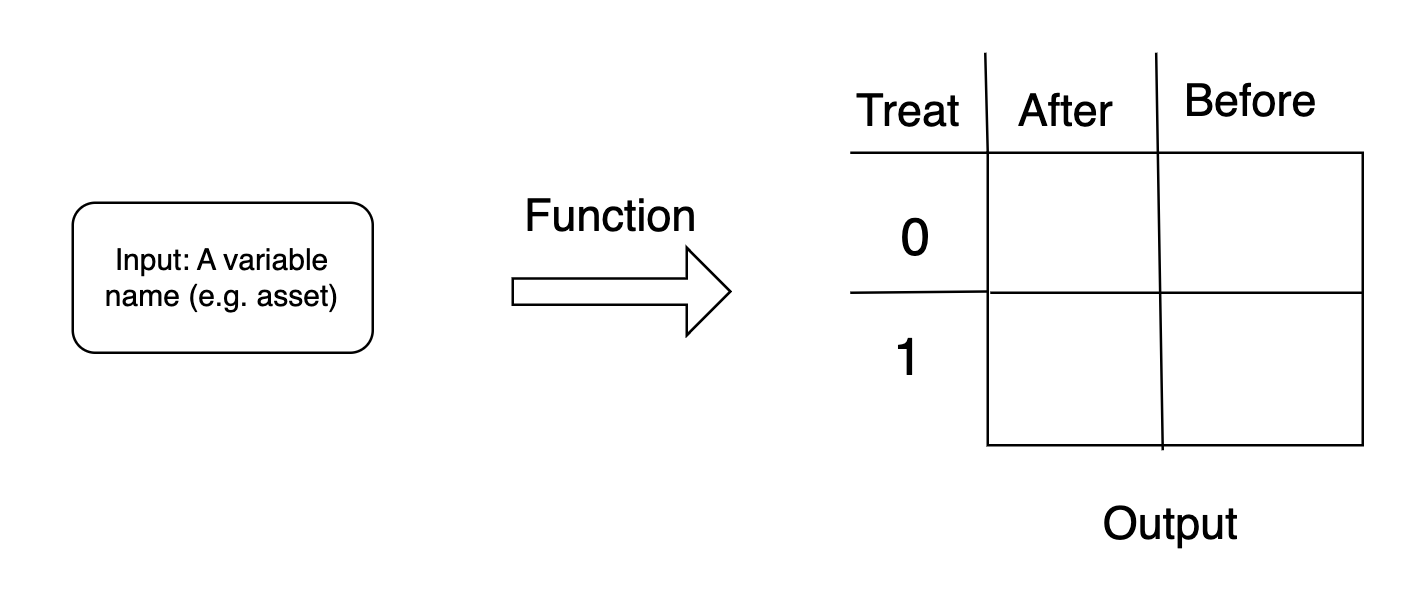
\includegraphics[width=0.75\linewidth]{images/10_function_ex} 

}

\caption{Goal for our Function}\label{fig:functionfigure}
\end{figure}

Instead of blanks in each cell, we will fill in with averages. So, for example, the cell in the top left is identified by treatment individuals after the policy has been implemented. If we supply the word \texttt{"asset"} to our function, then this first cell will be the average of \texttt{asset\_after} for individuals with \texttt{treat==1}. We know from the last section, this will be 791. For our function in this section, we want the function to automatically fill in all these numbers. In order to do so, we will need to understand how we can supply a single string (e.g.~``asset'') and then have R pull the relevant variables and then calculate the relevant means for both treated and control individuals.

Why might this be useful? Once we write our function, we can simply change the variable name and retrieve comparisons between treated and control individuals. There are a lot of variables in this dataset that cover a wide range of economic and psychological outcomes, so it may be helpful to have a function that can quickly perform this analysis for different variables.

To understand how this function will work, let's first write it for one variable: \texttt{asset}. Once we have this code written we can put it into a function to make it more general. To start, let's create an object named \texttt{variable} that is equal to the string \texttt{"asset"}.

\begin{Shaded}
\begin{Highlighting}[]
\NormalTok{variable }\OtherTok{\textless{}{-}} \StringTok{"asset"}
\end{Highlighting}
\end{Shaded}

Next, let's from our object \texttt{variable}, we want to create the variable names \texttt{asset\_after} and \texttt{asset\_before}, because these are the names of the variables in our dataset. To do this, we need to learn how to concatenate two strings. Concatenating strings simply means combining them. In other words, if I concatenate ``asset'' with ``\_after'' I get ``asset\_after''. The function that allows us to do this in R is called the \texttt{paste()} function. Let's see how this works:

\begin{Shaded}
\begin{Highlighting}[]
\NormalTok{variableafter }\OtherTok{\textless{}{-}} \FunctionTok{paste}\NormalTok{(variable,}\StringTok{"\_after"}\NormalTok{)}
\end{Highlighting}
\end{Shaded}

Now let's look at our new object:

\begin{Shaded}
\begin{Highlighting}[]
\NormalTok{variableafter}
\NormalTok{[}\DecValTok{1}\NormalTok{] }\StringTok{"asset \_after"}
\end{Highlighting}
\end{Shaded}

So if you look closely, you will see we actually have a problem. There is a space between \texttt{"asset"} and \texttt{"\_after"}. This is a problem. We will want to use \texttt{variableafter} to reference a particular column in our data frame. But there is no column named \texttt{"asset\ \_after"}. We need to tell \texttt{paste()} not to automatically add a space between our two strings. The way we can do this is by using an option called \texttt{sep=}. The option \texttt{sep=} stands for separator. It allows us to control what is put between two strings. If we want there to be no space between two strings, we can specify \texttt{sep=""}.

\begin{Shaded}
\begin{Highlighting}[]
\NormalTok{variableafter }\OtherTok{\textless{}{-}} \FunctionTok{paste}\NormalTok{(variable,}\StringTok{"\_after"}\NormalTok{,}\AttributeTok{sep=}\StringTok{""}\NormalTok{)}
\NormalTok{variableafter}
\NormalTok{[}\DecValTok{1}\NormalTok{] }\StringTok{"asset\_after"}
\end{Highlighting}
\end{Shaded}

So similarly, let's also construct \texttt{variablebefore}:

\begin{Shaded}
\begin{Highlighting}[]
\NormalTok{variablebefore }\OtherTok{\textless{}{-}} \FunctionTok{paste}\NormalTok{(variable,}\StringTok{"\_before"}\NormalTok{,}\AttributeTok{sep=}\StringTok{""}\NormalTok{)}
\NormalTok{variablebefore}
\NormalTok{[}\DecValTok{1}\NormalTok{] }\StringTok{"asset\_before"}
\end{Highlighting}
\end{Shaded}

Next, we want to get the average of these two variables for both the treated and control individuals. There are many ways we could approach this in R. Today, we are going to first construct two dataframes: one for treated individuals and one for control individuals. Then we are going to pull the relevant variables from the dataframes and take the average of these variables.

To start, let's separate out the treated and control data:

\begin{Shaded}
\begin{Highlighting}[]
\NormalTok{uct\_treat }\OtherTok{\textless{}{-}} \FunctionTok{filter}\NormalTok{(uct, treat}\SpecialCharTok{==}\DecValTok{1}\NormalTok{)}
\NormalTok{uct\_control }\OtherTok{\textless{}{-}} \FunctionTok{filter}\NormalTok{(uct, treat}\SpecialCharTok{==}\DecValTok{0}\NormalTok{)}
\end{Highlighting}
\end{Shaded}

Next, we are going to use the \texttt{pull()} function to grab the relevant columns. So this contrasts to other ways in which we have referenced variables with a dataframe. In the past, we have used either the \texttt{\$} operator or in tidyverse we used \texttt{select()} at times. The difference here is that our variable name is now in quotation marks. The value of \texttt{variablebefore} is \texttt{"asset\_before"}. If we used the dollar sign to reference this variable, we would type \texttt{uct\$asset\_before}, not \texttt{uct\$"asset\_before"}. Instead, we are going to use the \texttt{pull()} function, which allows us to use strings to reference variables. For example, to reference \texttt{asset\_after} in the \texttt{uct\_treat} data frame we can type \texttt{pull(uct\_treat,variableafter)}. If we want to take the mean of this, we can put the entire expression inside the \texttt{mean()} function.

\begin{Shaded}
\begin{Highlighting}[]
\FunctionTok{mean}\NormalTok{(}\FunctionTok{pull}\NormalTok{(uct\_treat,variableafter))}
\NormalTok{[}\DecValTok{1}\NormalTok{] }\FloatTok{790.9253}
\end{Highlighting}
\end{Shaded}

Now, let's repeat this process for the 3 remaining elements in the table that we want to create.

\begin{Shaded}
\begin{Highlighting}[]
\CommentTok{\# mean of variable after for control }
\FunctionTok{mean}\NormalTok{(}\FunctionTok{pull}\NormalTok{(uct\_control,variableafter))}
\NormalTok{[}\DecValTok{1}\NormalTok{] }\FloatTok{494.8041}

\CommentTok{\# mean of variable before for treatment }
\FunctionTok{mean}\NormalTok{(}\FunctionTok{pull}\NormalTok{(uct\_treat,variablebefore))}
\NormalTok{[}\DecValTok{1}\NormalTok{] }\FloatTok{382.3934}

\CommentTok{\# mean of variable before for control }
\FunctionTok{mean}\NormalTok{(}\FunctionTok{pull}\NormalTok{(uct\_control,variablebefore))}
\NormalTok{[}\DecValTok{1}\NormalTok{] }\FloatTok{389.371}
\end{Highlighting}
\end{Shaded}

For treated individuals, assets started at 382 and increased to 791. For control individuals, assets started at 389 and increased to 495. So while both groups saw an increase in assets over this time period, the treated individuals saw a much larger increase. This is evidence that the unconditional cash transfer is having a causal impact on savings.

We have now, successfully constructed the table, but only for assets. We want to be able to change the input each time and construct this for different variables. We could copy and paste the code above and repeat for different variables, but this will result in a long file of code which basically repeats the same process over and over. It will be much more efficient to put this code into a function.

Below we will display the function and then discuss the components:

\begin{Shaded}
\begin{Highlighting}[]
\NormalTok{treat.mean.var }\OtherTok{\textless{}{-}} \ControlFlowTok{function}\NormalTok{(variable)\{}
  
\NormalTok{  variableafter }\OtherTok{\textless{}{-}} \FunctionTok{paste}\NormalTok{(variable, }\StringTok{"\_after"}\NormalTok{, }\AttributeTok{sep=}\StringTok{""}\NormalTok{)}
\NormalTok{  variablebefore }\OtherTok{\textless{}{-}} \FunctionTok{paste}\NormalTok{(variable, }\StringTok{"\_before"}\NormalTok{, }\AttributeTok{sep=}\StringTok{""}\NormalTok{)}
  
  \CommentTok{\#Separate out control and treated data}
\NormalTok{  uct\_treat }\OtherTok{\textless{}{-}} \FunctionTok{filter}\NormalTok{(uct, treat}\SpecialCharTok{==}\DecValTok{1}\NormalTok{)}
\NormalTok{  uct\_control }\OtherTok{\textless{}{-}} \FunctionTok{filter}\NormalTok{(uct, treat}\SpecialCharTok{==}\DecValTok{0}\NormalTok{)}
  
  \CommentTok{\#Use the pull function }
  \CommentTok{\#Mean of variable after for treated}
\NormalTok{  treatafter }\OtherTok{\textless{}{-}} \FunctionTok{mean}\NormalTok{(}\FunctionTok{pull}\NormalTok{(uct\_treat, variableafter))}
  
  \CommentTok{\#Mean of variable after for control}
\NormalTok{  controlafter }\OtherTok{\textless{}{-}} \FunctionTok{mean}\NormalTok{(}\FunctionTok{pull}\NormalTok{(uct\_control, variableafter))}
  
  \CommentTok{\#Mean of variable before for treated}
\NormalTok{  treatbefore }\OtherTok{\textless{}{-}} \FunctionTok{mean}\NormalTok{(}\FunctionTok{pull}\NormalTok{(uct\_treat, variablebefore))}
  
  \CommentTok{\#Mean of variable before for control}
\NormalTok{  controlbefore }\OtherTok{\textless{}{-}} \FunctionTok{mean}\NormalTok{(}\FunctionTok{pull}\NormalTok{(uct\_control, variablebefore))}
  
  \CommentTok{\#Create output}
\NormalTok{  output }\OtherTok{\textless{}{-}} \FunctionTok{c}\NormalTok{(treatafter, treatbefore, controlafter, }
\NormalTok{              controlbefore)}
  \FunctionTok{names}\NormalTok{(output) }\OtherTok{\textless{}{-}} \FunctionTok{c}\NormalTok{(}\StringTok{"Treat After"}\NormalTok{, }\StringTok{"Treat Before"}\NormalTok{, }
                     \StringTok{"Control After"}\NormalTok{, }\StringTok{"Control Before"}\NormalTok{)}
  
  \FunctionTok{return}\NormalTok{(output)}
\NormalTok{\}}
\end{Highlighting}
\end{Shaded}

This is a function named \texttt{treat.mean.var} that takes \texttt{variable} as the input. We will pass in a variable from the data frame, for example \texttt{asset} or \texttt{nondurable\_expend}. Until we reach the line that starts with \texttt{output}, all of the code is exactly what we did before. The code subsets to two separate dataframes, one for treated individuals and one for control individuals, and then calculates the mean of the variable both before and after the program.

The remaining code simply puts together the output in a way we will be able to understand. The line \texttt{output\ \textless{}-\ c(treatafter,treatbefore,\ controlafter,\ controlbefore)} takes the four means and puts them into a single vector. The code \texttt{names(output)\textless{}-\ c("Treat\ After",\ "Treat\ Before",\ "Control\ After",\ "Control\ Before")} is associating each entry in the vector with a name. This will allow us to understand what the function is presenting us without having to look through the function to figure it out everytime we execute it.

Let's give this new function a try using \texttt{"asset"} as the input:

\begin{Shaded}
\begin{Highlighting}[]
\FunctionTok{treat.mean.var}\NormalTok{(}\StringTok{"asset"}\NormalTok{)}
\NormalTok{   Treat After   Treat Before  Control After Control Before }
      \FloatTok{790.9253}       \FloatTok{382.3934}       \FloatTok{494.8041}       \FloatTok{389.3710} 
\end{Highlighting}
\end{Shaded}

Now that we have our function set up, let's look at another variable: nondurable expenditure. Nondurable expenditure are goods that are consumed over a short time period. For example, food is a common nondurable good.

\begin{Shaded}
\begin{Highlighting}[]
\FunctionTok{treat.mean.var}\NormalTok{(}\StringTok{"nondurable\_expend"}\NormalTok{)}
\NormalTok{   Treat After   Treat Before  Control After Control Before }
      \FloatTok{191.2080}       \FloatTok{174.3455}       \FloatTok{157.6120}       \FloatTok{183.5800} 
\end{Highlighting}
\end{Shaded}

In the treatment, nondurable expenditures went up from 174 to 191. In contrast, in the control, nondurable expenditures actually decreased, starting at 184 and then falling to 158. Therefore, it appears unconditional cash transfers also had an impact on the amount individuals were spending on nondurable consumption.

Haushofer and Shapiro (2016) have a variety of other outcomes they measure. Now that we've written a function to do our analysis, we can quickly perform the analysis across these different variables. This is how functions can save you time when performing data analysis, and also improve the clarity of the code you do write, by making it more concise.

\section{Conclusion}\label{conclusion-8}

In this section we are going to wrap up functions by reviewing how to construct them in R. We will perform a similar analysis as the previous section, however, in this section we will use linear regression to analyze the data. To set up our analysis, let's first write out the regression equation we will estimate:

\[
Y_i = \beta_0 + \beta_1 \cdot Treat_i + \varepsilon_i
\]

Our dependent variable will be the change in an outcome. For example, if we are interested in understanding how the treatment has impacted the change in assets for a household, then we will set \(Y_i\) to be equal to \texttt{asset\_after-asset\_before}. We will estimate \(\hat{\beta}_1\) which gives us the differential change in assets between treated and control individuals. For example, if \(\hat{\beta}_1=100\), then that indicates treated individuals experienced a larger increase in assets than individuals in the control group. For example, it could be that the control group experienced a 200 increase in assets over the two time periods we are studying, while the treated group experienced a 300 increase in assets over the two time periods. In this case, assets went up by 100 more in the treated group relative to the control group.

In this study, we have a number of variables that are in the format \texttt{variable\_after} and \texttt{variable\_before}. Instead of doing the linear regression with different variable names, we are instead going to write in a function that takes as an input ``\texttt{variable\textquotesingle{}\textquotesingle{}}, and then estimates the regression for this variable.

To understand how we will build the function, let's first estimate this regression for \texttt{asset}. That will give us an idea how we can do this more generally in a function. First, we need to create our \(Y_i\) variable, which is equal to \texttt{asset\_after-asset\_before}.

\begin{Shaded}
\begin{Highlighting}[]
\NormalTok{y }\OtherTok{\textless{}{-}}\NormalTok{ uct}\SpecialCharTok{$}\NormalTok{asset\_after}\SpecialCharTok{{-}}\NormalTok{uct}\SpecialCharTok{$}\NormalTok{asset\_before}
\end{Highlighting}
\end{Shaded}

Note, we have not added our new variable \texttt{y} to our dataframe. It is currently a vector in our global environment. In all our previous examples, we have estimated a linear regression on variables within a dataframe. In this section, we will show you can also estimate linear regression on a pair of vectors. To do so, let's create a vector \texttt{treat} which is the same as the variable \texttt{treat} within the dataframe \texttt{uct}.

\begin{Shaded}
\begin{Highlighting}[]
\NormalTok{treat }\OtherTok{\textless{}{-}}\NormalTok{ uct}\SpecialCharTok{$}\NormalTok{treat}
\end{Highlighting}
\end{Shaded}

Now we can estimate the linear regression. Unlike most of the prior \texttt{lm()} models we have estimated, we do not need to specify the dataframe, as we are now directly utilizing vectors in our global environment. One could have done this by adding \texttt{y} to our dataframe as usual, but this illustration shows an alternative way to accomplish the same analysis.

\begin{Shaded}
\begin{Highlighting}[]
\NormalTok{lm}\FloatTok{.1} \OtherTok{\textless{}{-}} \FunctionTok{lm}\NormalTok{(y }\SpecialCharTok{\textasciitilde{}}\NormalTok{ treat)}
\NormalTok{lm}\FloatTok{.1}

\NormalTok{Call}\SpecialCharTok{:}
\FunctionTok{lm}\NormalTok{(}\AttributeTok{formula =}\NormalTok{ y }\SpecialCharTok{\textasciitilde{}}\NormalTok{ treat)}

\NormalTok{Coefficients}\SpecialCharTok{:}
\NormalTok{(Intercept)        treat  }
      \FloatTok{105.4}        \FloatTok{303.1}  
\end{Highlighting}
\end{Shaded}

We see that the slope coefficient \(\hat{\beta}_1 = 303.10\). This tells us that the treated group experienced an additional 303 dollar gain relative to the control group. If we look at the intercept, we know in this case this is the expected gain for individuals in the control group. In other words, individuals in the control group experienced a 105 dollar increase in assets. However, the slope coefficient tells us that the treated individuals experienced an additional 303 dollar gain, for a total gain of (105+303=408).

Now let's do this more generally using strings. Again, let's start by creating a string object called \texttt{variable} that is equal to \texttt{"asset"}.

\begin{Shaded}
\begin{Highlighting}[]
\NormalTok{variable  }\OtherTok{\textless{}{-}} \StringTok{"asset"}
\end{Highlighting}
\end{Shaded}

Next, let's use \texttt{paste} to create \texttt{"asset\_before"} and \texttt{"asset\_after"}.

\begin{Shaded}
\begin{Highlighting}[]
\NormalTok{variableafter }\OtherTok{\textless{}{-}} \FunctionTok{paste}\NormalTok{(variable, }\StringTok{"\_after"}\NormalTok{,}\AttributeTok{sep=}\StringTok{""}\NormalTok{)}
\NormalTok{variablebefore }\OtherTok{\textless{}{-}} \FunctionTok{paste}\NormalTok{(variable, }\StringTok{"\_before"}\NormalTok{,}\AttributeTok{sep=}\StringTok{""}\NormalTok{)}
\end{Highlighting}
\end{Shaded}

Now we can create our \(Y_i\) which is equal to \texttt{asset\_after-asset\_before}. Again we can use the \texttt{pull()} function to grab the columns of the dataframe with the corresponding variable names:

\begin{Shaded}
\begin{Highlighting}[]
\NormalTok{y }\OtherTok{\textless{}{-}} \FunctionTok{pull}\NormalTok{(uct,variableafter) }\SpecialCharTok{{-}} \FunctionTok{pull}\NormalTok{(uct,variablebefore)}
\NormalTok{treat }\OtherTok{\textless{}{-}} \FunctionTok{pull}\NormalTok{(uct,treat)}
\end{Highlighting}
\end{Shaded}

Now we can run our linear regression just as before:

\begin{Shaded}
\begin{Highlighting}[]
\NormalTok{lm}\FloatTok{.1} \OtherTok{\textless{}{-}} \FunctionTok{lm}\NormalTok{(y }\SpecialCharTok{\textasciitilde{}}\NormalTok{ treat)}
\NormalTok{lm}\FloatTok{.1}

\NormalTok{Call}\SpecialCharTok{:}
\FunctionTok{lm}\NormalTok{(}\AttributeTok{formula =}\NormalTok{ y }\SpecialCharTok{\textasciitilde{}}\NormalTok{ treat)}

\NormalTok{Coefficients}\SpecialCharTok{:}
\NormalTok{(Intercept)        treat  }
      \FloatTok{105.4}        \FloatTok{303.1}  
\end{Highlighting}
\end{Shaded}

We have now figured out how to pass a string \texttt{"asset"} to an object named \texttt{variable} and perform the analysis. Therefore, we need to make only a few small changes to put this code into a function. We will name our function \texttt{lm.var} because it will perform a linear regression on an input variable.

\begin{Shaded}
\begin{Highlighting}[]
\NormalTok{lm.var }\OtherTok{\textless{}{-}} \ControlFlowTok{function}\NormalTok{(variable)\{}
  
  \CommentTok{\#Create a before and after variable}
\NormalTok{  variableafter }\OtherTok{\textless{}{-}} \FunctionTok{paste}\NormalTok{(variable, }\StringTok{"\_after"}\NormalTok{, }\AttributeTok{sep=}\StringTok{""}\NormalTok{)}
\NormalTok{  variablebefore }\OtherTok{\textless{}{-}} \FunctionTok{paste}\NormalTok{(variable, }\StringTok{"\_before"}\NormalTok{, }\AttributeTok{sep=}\StringTok{""}\NormalTok{)}
  
  \CommentTok{\#Create a y variable}
\NormalTok{  y }\OtherTok{\textless{}{-}} \FunctionTok{pull}\NormalTok{(uct, variableafter) }\SpecialCharTok{{-}} \FunctionTok{pull}\NormalTok{(uct, variablebefore)}
\NormalTok{  treat }\OtherTok{\textless{}{-}} \FunctionTok{pull}\NormalTok{(uct, treat)}
  
  \CommentTok{\#Run the linear regression}
\NormalTok{  lm}\FloatTok{.1} \OtherTok{\textless{}{-}} \FunctionTok{lm}\NormalTok{(y }\SpecialCharTok{\textasciitilde{}}\NormalTok{ treat)}
  \FunctionTok{return}\NormalTok{(lm}\FloatTok{.1}\NormalTok{)}
\NormalTok{\}}
\end{Highlighting}
\end{Shaded}

To review, the first line \texttt{lm.var\ \textless{}-\ function(variable)\ \{} specifies a few things. First, the name of the function is \texttt{lm.var}. Second, the \texttt{function} tells R that we are creating a new function. \texttt{variable} will be the name of the input. This is what we will change each time we execute the function. To make sure this works, let's use this on \texttt{"asset"}. We have already performed this analysis so we know what it should return.

\begin{Shaded}
\begin{Highlighting}[]
\FunctionTok{lm.var}\NormalTok{(}\StringTok{"asset"}\NormalTok{)}

\NormalTok{Call}\SpecialCharTok{:}
\FunctionTok{lm}\NormalTok{(}\AttributeTok{formula =}\NormalTok{ y }\SpecialCharTok{\textasciitilde{}}\NormalTok{ treat)}

\NormalTok{Coefficients}\SpecialCharTok{:}
\NormalTok{(Intercept)        treat  }
      \FloatTok{105.4}        \FloatTok{303.1}  
\end{Highlighting}
\end{Shaded}

It appears our function is working properly. Now, we can repeat this analysis on many different variables. For example, let's see what this looks like for \texttt{total\_rev}.

\begin{Shaded}
\begin{Highlighting}[]
\FunctionTok{lm.var}\NormalTok{(}\StringTok{"total\_rev"}\NormalTok{)}

\NormalTok{Call}\SpecialCharTok{:}
\FunctionTok{lm}\NormalTok{(}\AttributeTok{formula =}\NormalTok{ y }\SpecialCharTok{\textasciitilde{}}\NormalTok{ treat)}

\NormalTok{Coefficients}\SpecialCharTok{:}
\NormalTok{(Intercept)        treat  }
      \SpecialCharTok{{-}}\FloatTok{39.9}         \FloatTok{49.0}  
\end{Highlighting}
\end{Shaded}

Again, we see a positive impact for treated households. We see a bigger increase in the treated group in terms of household revenue relative to the control group.

Concept check: Try this out for \texttt{nondurable\_expend} and \texttt{food\_security} and make sure you understand the resulting output.

In this section, we studied the effect of unconditional cash transfers on households in Kenya using data from Haushofer and Shapiro (2016). A key strength of Haushofer and Shapiro is the ability to collect a wide variety of outcomes. Their paper allows us to understand how unconditional cash transfers impact not only economic well being, but also psychological well being.
This paper relates to a broader and burgeoning literature on universal basic income (UBI). The merits of UBI have been debated intensely, in politics, the popular press, and in academia. The basic concept of UBI is that individuals receive a guaranteed cash payment. This will guarantee individuals a certain level of income, but some fear will lead to worse economic outcomes if individuals choose to reduce work.

To date, there are very few examples of UBI payments that occur at a large scale for an extended time. For example, in Haushofer and Shapiro (2016), the authors give payments to a few hundred households over the course of about a year. However, through the same charity, GiveDirectly, researchers are currently implementing a large-scale UBI program in rural Kenya (see Banerjee et al.~2020). In this program, researchers are providing entire villages in rural Kenya with a universal basic income experiment for 12 years. The results of such a large-scale experiment will be tremendously informative regarding the pros and cons of UBI.

\section*{Function Descriptions}\label{function-descriptions-4}
\addcontentsline{toc}{section}{Function Descriptions}

\textbf{Functions Used}

\begin{itemize}
\item
  \texttt{paste()} -- Concatenates strings together. For example, \texttt{paste("Hello","World")} results in the text ``Hello World''.
\item
  \texttt{pull()} -- Extracts columns from a dataframe. For example, given a dataframe \texttt{df} and a variable \texttt{varname}, we can extract the variable by specifying, \texttt{pull(df,"varname")}.
\item
  \texttt{function()} -- Function to specify a new function in R.
\end{itemize}

\chapter*{References}\label{references-1}
\addcontentsline{toc}{chapter}{References}

\bibliography{book.bib,packages.bib}

\end{document}
